%%% ====================================================================
%%%  @LaTeX-file{
%%%     author          = "Scott Pakin",
%%%     version         = "14.0",
%%%     date            = "05 May 2021",
%%%     time            = "16:10:48 MDT",
%%%     filename        = "symbols.tex",
%%%     checksum        = "49890 24745 81503 1177698",
%%%     email           = "scott+clsl@pakin.org (Internet)",
%%%     codetable       = "ISO/ASCII",
%%%     keywords        = "symbols, LaTeX2e, typesetting, accents,
%%%                        mathematics, scientific, dingbats, fonts",
%%%     supported       = "yes",
%%%     abstract        = "This document lists thousands of symbols and
%%%                        the corresponding LaTeX commands that
%%%                        produce them.  Some of these symbols are
%%%                        guaranteed to be available in every LaTeX2e
%%%                        system; others require fonts and packages
%%%                        that may not accompany a given distribution
%%%                        and that therefore need to be installed.
%%%                        All of the fonts and packages used to
%%%                        prepare this document -- as well as this
%%%                        document itself -- are freely available
%%%                        from the Comprehensive TeX Archive Network
%%%                        (http://www.ctan.org).",
%%%     docstring       = "This LaTeX document showcases thousands of
%%%                        symbols that are available to authors.  The
%%%                        original version of this document was
%%%                        written by David Carlisle on 1994/10/02.
%%%                        It was subsequently changed and expanded by
%%%                        Scott Pakin.
%%%
%%%                        To build this document, run ``latex
%%%                        symbols'', then ``makeindex -s gind.ist
%%%                        symbols'', then two more ``latex symbols''
%%%                        commands.  This ensures the stability of
%%%                        all generated content (tables, references,
%%%                        etc.)
%%%
%%%                        The checksum field above contains a CRC-16
%%%                        checksum as the first value, followed by
%%%                        the equivalent of the standard UNIX wc
%%%                        (word count) utility output of lines,
%%%                        words, and characters.  This is produced by
%%%                        Robert Solovay's checksum utility.  This file
%%%                        header was produced with the help of Nelson
%%%                        Beebe's filehdr utility.  Both checksum and
%%%                        filehdr are available from CTAN
%%%                        (http://www.ctan.org)."
%%%  }
%%% ====================================================================

\NeedsTeXFormat{LaTeX2e}
\IfFileExists{cmap.sty}{\RequirePackage[resetfonts]{cmap}}{}
\documentclass{article}
\usepackage{array}
\usepackage{longtable}
\usepackage{textcomp}
\usepackage{fakelatexsym}
\usepackage{varioref}
\usepackage{xspace}
\usepackage{makeidx}
\usepackage{verbatim}
\usepackage{graphicx}
\usepackage{ifpdf}
\usepackage{tabularx}
\usepackage{keyval}

\newcommand{\doctitle}{Comprehensive \LaTeX\ Symbol List}  % Reusable
\title{The \doctitle}

\author{\person{Scott}{Pakin} \texttt{<scott+clsl@pakin.org>}%
  \thanks{The original version of this document was written by
    \person{David}{Carlisle}, with several additional tables provided
    by \person{Alexander}{Holt}.  See \vref{about-doc} for more
    information about who did what.}}
\date{5 May 2021}

\makeindex

%%%
%%% TO-DO LIST
%%%   * Proofread, especially looking for symbols defined by more
%%%     than one symbol set or symbols that should be in a table
%%%     but aren't.
%%%   * Add more symbol tables.  (Did we miss any common, standard, or
%%%     useful ones?)
%%%   * Further index symbols by _description_ (e.g., "perpendicular"
%%%     for "\perp").  This would be really useful, but extremely
%%%     time-consuming to do.  Note that Adobe's Web site has a list
%%%     of the names of all the Zapf Dingbats characters.  Unfortunately,
%%%     these names can be rather long, like "notched upper right-shadowed
%%%     white rightwards arrow" for \ding{241}.
%%%   * Find some way to associate each package with a flag indicating
%%%     whether the corresponding fonts are in bitmapped or vector
%%%     format.
%%%   * Verify that there aren't any missing symbols in the current
%%%     packages (especially after font upgrades).
%%%   * Reduce the amount of duplication, in particular with regard to
%%%     large math fonts that all define \subset, \supset, \prec, \succ,
%%%     etc.  Perhaps include a canonical table then have other fonts
%%%     refer back to that, showing samples only of more unique characters.
%%%

% Index "X Y" and "Y, X".  The "begin" and "end" variants are for page ranges.
\newcommand{\idxboth}[2]{\mbox{}\index{#1 #2}\index{#2>#1}\index{#2}}
\newcommand{\idxbothbegin}[2]{\mbox{}\index{#1 #2|(}\index{#2>#1|(}\index{#2|(}}
\newcommand{\idxbothend}[2]{\mbox{}\index{#1 #2|)}\index{#2>#1|)}\index{#2|)}}

% Index package names and hyperlink them to the CTAN package information.
% An optional argument of "index=false" suppresses indexing the package name.
% An optional argument of "pkg=<name>" uses package <name> for the CTAN
% hyperlink target.
% An optional argument of "link=<URL>" replaces the whole hyperlink with <URL>.
% An optional argument of "nolink" suppresses the hyperlink entirely.
% An optional argument of "fmt=<code>" typesets the package name using <code>.
% The package name must be pure text.  Use "fmt=<code>" for special formatting.
% Define \pkgnameopts as the default options for all subsequent calls.
% Use \setpkgnameopts to set the default options for a specific package.
\def\equalsign{=}
\newcommand*{\catalogueURL}[1]{%
  http://www.ctan.org/pkg/#1%
}
\makeatletter
\define@key{pkgname}{pkg}{\def\pkglinktarget{#1}}
\define@key{pkgname}{link}{\def\catalogueURL##1{#1}}
\define@key{pkgname}{nolink}[true]{\def\pkglink##1{\pkgnamefmt{##1}}}
\define@key{pkgname}{index}[true]{\csname pkgidx#1\endcsname}
\define@key{pkgname}{fmt}{\def\pkgnamefmt##1{#1}}
\def\pkgnameopts{}
\newcommand{\setpkgnameopts}[2]{%
  \expandafter\gdef\csname pkgnameopts@#1\endcsname{#2}%
}
\makeatother
\newif\ifpkgidx
\newcommand{\pkgname}[2][]{%
  \bgroup
    \def\pkglinktarget{#2}%
    \def\pkgnamefmt##1{\textsf{##1}}%
    \def\pkglink##1{\href{\catalogueURL{\pkglinktarget}}{\pkgnamefmt{##1}}}%
    \pkgidxtrue
    \edef\next{\noexpand\setkeys{pkgname}{\pkgnameopts}}\next
    \expandafter\ifx\csname pkgnameopts@#2\endcsname\relax
    \else
      \edef\next{\noexpand\setkeys{pkgname}{\csname pkgnameopts@#2\endcsname}}%
      \next
    \fi
    \setkeys{pkgname}{#1}%
    \pkglink{#2}%
    \ifpkgidx
      \def\equalsign{!=}%   % Escape the equals sign for makeindex's sake.
      \index{#2=\pkglink{#2} (package)}%
      \index{packages>#2=\pkglink{#2}}%
    \fi
  \egroup
}

% Index some other logical styles.
\newcommand{\optname}[2]{%
  \textsf{#2}%
  \index{#2=\textsf{#2} (\textsf{#1} package option)}%
  \index{package options>#2=\textsf{#2} (\textsf{#1})}}
\newcommand{\filename}[1]{%
  \texttt{#1}%
  \index{#1=\texttt{#1} (file)}}
\newcommand{\hfilename}[2]{%
  \href{#1}{\texttt{#2}}%
  \index{#2=\noexpand\href{#1}{\noexpand\texttt{#2}} (file)}}
\newcommand{\fileext}[1]{%
  \texttt{.#1}%
  \index{#1 files=\texttt{.#1} files}%
  \index{file extensions>#1=\texttt{.#1}}%
}
\newcommand{\PSfont}[1]{%
  #1%
  \index{#1 (font)}%
  \index{fonts>#1}%
}
\DeclareRobustCommand{\person}[2]{#1\index{#2, #1} #2}

% Index common words and phrases.
\newcommand{\latex}{\LaTeX\index{LaTeX=\string\LaTeX}\xspace}
\newcommand{\latexE}{\LaTeXe\index{LaTeX2e=\string\LaTeXe}\xspace}
\newcommand{\metafont}{\MF\index{Metafont=\string\MF}\xspace}
\newcommand{\tex}{\TeX\index{TeX=\string\TeX}\xspace}
\newcommand{\xypic}{%
  \mbox{\kern-.1em X\kern-.3em\lower.4ex\hbox{Y\kern-.15em}-pic}%
  \index{Xy-pic=\mbox{\kern-.1em X\kern-.3em\lower.4ex\hbox{Y\kern-.15em}-pic}}}
\newcommand{\TeXbook}{%
  The \TeX{}book\index{TeXbook, The=\TeX{}book, The}~\cite{Knuth:ct-a}\xspace}
\newcommand{\ctt}{%
  \texttt{comp.text.tex}%
  \index{comp.text.tex=\texttt{comp.text.tex} (newsgroup)}\xspace}
\newcommand{\fntenc}[1][]{%
  \def\firstarg{#1}%
  font encoding%
  \index{font encodings}%
  \ifx\firstarg\empty
  \else
    \index{font encodings>\firstarg}%
  \fi
}
\newcommand{\fntfam}[1][]{%
  \def\firstarg{#1}%
  font family%
  \index{font families}%
  \ifx\firstarg\empty
  \else
    \index{font families>\firstarg=\string\texttt{\firstarg}}%
  \fi
}
\newcommand{\selftex}{\hfilename{http://mirror.ctan.org/info/symbols/comprehensive/source/symbols.tex}{symbols.tex}\xspace}
\newcommand{\fontdefdtx}{\hfilename{http://mirror.ctan.org/macros/latex/base/fontdef.dtx}{fontdef.dtx}\xspace}
\newcommand{\testfonttex}{\hfilename{http://mirror.ctan.org/macros/plain/base/testfont.tex}{testfont.tex}\xspace}
\newcommand{\TUGboat}{%
  \href{http://www.tug.org/TUGboat/}{TUGboat}%
  \index{TUGboat=\href{http://www.tug.org/TUGboat/}{TUGboat}}\xspace
}
\newcommand{\thanhhanthe}{Th\`anh, H\`an Th\diatop[\'|\^e]}   % "|" confuses MakeIndex.
\newcommand{\postscript}{PostScript\index{PostScript}\xspace}
\newcommand{\ascii}{ASCII\index{ASCII}\xspace}
\newcommand{\utfviii}{\mbox{UTF-8}\index{UTF-8}\xspace}
\DeclareRobustCommand{\xelatexInternal}{%
  \mbox{X\lower0.5ex\hbox{\kern-0.15em\reflectbox{E}}\kern-0.1em\LaTeX}}
\newcommand{\xelatex}{\xelatexInternal\index{XeLaTeX=\string\xelatexInternal}\xspace}
\DeclareRobustCommand{\xetexInternal}{%
  \mbox{X\lower0.5ex\hbox{\kern-0.15em\reflectbox{E}}\kern-0.1em\TeX}}
\newcommand{\xetex}{\xetexInternal\index{XeTeX=\string\xetexInternal}\xspace}
\newcommand{\lualatex}{Lua\LaTeX\index{LuaLaTeX=Lua\string\LaTeX}\xspace}
\newcommand{\italic}[1][italic]{#1\index{italic}}
\newcommand{\TikZ}{\pkgname{TikZ}}
\setpkgnameopts{TikZ}{pkg=pgf,fmt={Ti\noexpand\textit{k}Z}}
\newcommand{\PSTricks}{\pkgname{PSTricks}}
\setpkgnameopts{PSTricks}{pkg=pstricks-base}
\newcommand{\rawtables}{Raw\index{Raw Font Tables} Font Tables}

% Index TeXbook symbols and the CTAN repository.
\newcommand{\idxTBsyms}{%
  \index{symbols>TeXbook=\TeX{}book}%
  \index{TeXbook, The=\TeX{}book, The>symbols from}%
}
\newcommand{\idxCTAN}{%
  \index{Comprehensive TeX Archive Network=\href{http://www.ctan.org/}{Comprehensive \string\TeX{} Archive Network}}%
}
\newcommand{\CTAN}{\href{http://www.ctan.org/}{CTAN}\idxCTAN\xspace}
\newcommand{\CTANfull}{Comprehensive\idxCTAN\ \TeX\ Archive Network\xspace}
\newcommand{\TeXFAQ}[1]{\url{http://www.tex.ac.uk/FAQ-#1.html}}


%%%%%%%%%%%%%%%%%%%%%%%%%%%%%%%%%%%%%%%%%%%%%%%%%%%%%%%%%%%%%%%%%%%%%%%%%%
% There are a number of symbols (e.g., \Square) that are defined by      %
% multiple packages.  In order to typeset all the variants in this       %
% document, we have to give glyph a unique name.  To do that, we define  %
% \savesymbol{XXX}, which renames a symbol from \XXX to \origXXX, and    %
% \restoresymbol{yyy}{XXX}, which renames \origXXX back to \XXX and      %
% defines a new command, \yyyXXX, which corresponds to the most recently %
% loaded version of \XXX.                                                %
%                                                                        %
% This implementation of \savesymbol and \restoresymbol was copied from  %
% the savesym package, which started with symbol.tex's old definitions   %
% of those macros and improved upon them.  However, \renamerobustsymbol  %
% and \ifnotsavedsym are new to this set.                                %
%                                                                        %

% Save a symbol that we know is going to get redefined.
\newcommand*{\savesymbol}[1]{%
  \expandafter\let\csname orig#1\expandafter\endcsname\csname#1\endcsname
  \expandafter\let\csname #1\endcsname\relax
}

% Restore a previously saved symbol, and rename the current one.
\newcommand*{\restoresymbol}[2]{%
  \expandafter\global\expandafter\let\csname#1#2\expandafter\endcsname%
    \csname#2\endcsname
  \expandafter\global\expandafter\let\csname#2\expandafter\endcsname%
    \csname orig#2\endcsname
}

% Rename a robust command.
\newcommand*{\renamerobustsymbol}[2]{%
  \expandafter\let\expandafter\origrealcommand
    \csname #2\space\endcsname
  \expandafter\global\expandafter\let\csname#1#2\endcsname=\origrealcommand
}

% Test if a symbol is not saved.
\makeatletter
\def\ifnotsavedsym@helper#1#2!{\expandafter\ifx\csname orig#2\endcsname\relax}
\newcommand*{\ifnotsavedsym}[1]{%
  \expandafter\ifnotsavedsym@helper\string#1!%
}
\makeatother
%                                                                        %
%%%%%%%%%%%%%%%%%%%%%%%%%%%%%%%%%%%%%%%%%%%%%%%%%%%%%%%%%%%%%%%%%%%%%%%%%%


% Each of the packages used by this document is loaded conditionally.
% However, it might be nice to know if we have a complete set.  So we
% define \ifcomplete which starts true, but gets set to false if any
% package is missing.
\newif\ifcomplete
\completetrue

% For debugging purposes we define a switch that enables us to toggle
% on and off the loading of packages.
\newif\ifloadpackages
\loadpackagestrue

% \IfStyFileExists* is just like \IfFileExists, except that it appends
% ".sty" to its first argument.  \IfStyFileExists is the same as
% \IfStyFileExists*, but it additionally adds its first argument to a
% list (\missingpkgs) and marks the document as incomplete (with
% \completefalse) if the .sty file doesn't exist.  \IfPackageFileExists
% is the same as \IfStyFileExists except that it separates the package
% name from a file within the package (not necessarily a .sty file) for
% which to search.
\makeatletter
\newcommand{\missingpkgs}{}
\newcommand{\foundpkgs}{}
\newcommand{\if@sty@file@exists@star}[3]{%
  \ifloadpackages
    \IfFileExists{#1.sty}{#2}{#3}%
  \else
    #3%
  \fi
}
\newcommand{\if@sty@file@exists}[3]{%
  \ifloadpackages
    \IfFileExists{#1.sty}%
                 {#2\@cons\foundpkgs{{#1}}}%
                 {#3\completefalse\@cons\missingpkgs{{#1}}}%
  \else
    #3\completefalse\@cons\missingpkgs{{#1}}%
  \fi
}
\newcommand{\IfStyFileExists}{%
  \@ifstar{\if@sty@file@exists@star}{\if@sty@file@exists}%
}
\newcommand{\IfPackageFileExists}[4]{%
  \ifloadpackages
    \IfFileExists{#2}%
                 {#3\@cons\foundpkgs{{#1}}}%
                 {#4\completefalse\@cons\missingpkgs{{#1}}}%
  \else
    #4\completefalse\@cons\missingpkgs{{#1}}%
  \fi
}
\makeatother

% We get a few packages for free.
\makeatletter
\@cons\foundpkgs{{textcomp}}
\@cons\foundpkgs{{latexsym}}
\makeatother
\newcommand{\TC}{\pkgname{textcomp}}
\setpkgnameopts{latexsym}{link=http://www.ctan.org/pkg/latex-base}

% Load etex if possible to increase the number of various TeX resources
% we have available.
\IfStyFileExists*{etex}{\usepackage{etex}}{}

% Typeset a string in various encodings.
\newcommand{\encone}[1]{{\fontencoding{T1}\selectfont#1}}
\newcommand{\enctwoA}[1]{{\fontencoding{T2A}\selectfont#1}}
\newcommand{\encfour}[1]{{\fontencoding{T4}\selectfont#1}}
\newcommand{\encfive}[1]{{\fontencoding{T5}\selectfont#1}}
\newcommand{\encgreek}[1]{{\fontencoding{LGR}\selectfont#1}}

% Various punctuation marks confuse makeindex when used directly.
\let\magicrbrack=]
\let\magicequal=\=
\DeclareRobustCommand{\magicequalname}{\texttt{\string\=}}
\DeclareRobustCommand{\magicvertname}{\texttt{|}}
\DeclareRobustCommand{\magicVertname}{\texttt{\string\|}}

% Vertically center a text-mode symbol.
\newsavebox{\tvcbox}
\newcommand*{\textvcenter}[1]{%
  \savebox{\tvcbox}{#1}%
  \raisebox{0.5\dp\tvcbox}{\raisebox{-0.5\ht\tvcbox}{\usebox{\tvcbox}}}%
}

% Do the same work as \DeclareTextSymbol but only if the symbol is not
% already declared.
\let\origDeclareTextSymbol=\DeclareTextSymbol
\DeclareRobustCommand{\DeclareNewTextSymbol}[3]{%
  \ifnotsavedsym{#1}%
    \origDeclareTextSymbol{#1}{#2}{#3}%
  \fi
}

% Do the same work as \DeclareTextCommand but only if the symbol is not
% already declared.
\let\origDeclareTextCommand=\DeclareTextCommand
\DeclareRobustCommand{\DeclareNewTextCommand}[3]{%
  \ifnotsavedsym{#1}%
    \origDeclareTextCommand{#1}{#2}{#3}%
  \fi
}

% Define a helper function for \CLSL@fake@tdelim and \CLSL@fake@ddelim below.
\makeatletter
\def\CLSL@char@in@box#1{%
  \setbox0=\hbox{\char#1}%
  \hbox{%
    \vrule width \wd0 height 0pt depth 0pt%
    \vrule width 0pt height \ht0 depth \dp0%
    \smash{\box0}%
  }%
  \vspace*{-1pt}% Why is this necessary?
}
\makeatother

% Construct a text-sized delimiter from its constituent characters.
\makeatletter
\DeclareRobustCommand{\CLSLfaketdelim}[3]{%
  \begingroup
    \offinterlineskip
    \vbox{%
      \halign{##\cr
        \CLSL@char@in@box{#1}\cr  % top
        \CLSL@char@in@box{#2}\cr  % mid
        \CLSL@char@in@box{#3}\cr  % bot
      }%
    }%
  \endgroup
}
\makeatother

% Construct a display-sized delimiter from its constituent characters.
\makeatletter
\newcounter{CLSL@reps@left}
\DeclareRobustCommand{\CLSLfakeddelim}[5][2]{%
  \begingroup
    \offinterlineskip
    \vbox to 4ex{%
      \halign{##\cr
        \CLSL@char@in@box{#2}\cr     % top
        \setcounter{CLSL@reps@left}{#1}%
        \gdef\CLSL@reps{}
        \loop
          \g@addto@macro\CLSL@reps{\CLSL@char@in@box{#5}\cr}%
          \addtocounter{CLSL@reps@left}{-1}%
          \ifnum\c@CLSL@reps@left>0%
        \repeat
        \CLSL@reps                % rep
        \CLSL@char@in@box{#3}\cr  % mid
        \gdef\CLSL@reps{}
        \loop
          \g@addto@macro\CLSL@reps{\CLSL@char@in@box{#5}\cr}%
          \addtocounter{CLSL@reps@left}{-1}%
          \ifnum\c@CLSL@reps@left>0%
        \repeat
        \CLSL@reps                % rep
        \CLSL@char@in@box{#4}\cr  % bot
      }%
      \vss
    }%
  \endgroup
}
\makeatother

% Given a math expression, a small accent character, and a large
% accent character, typeset the expression with the appropriate-sized
% accent above it.
\DeclareRobustCommand{\CLSLfakewidetopaccent}[6]{%
  \setbox0=\hbox{\ensuremath{#1}}%
  \setbox1=\hbox{\ensuremath{abc}}%
  \mbox{\itshape#1}%
  \ifdim\wd0<\wd1
    \llap{\raisebox{#2}{\makebox[\wd0]{\usefont#6\char#3}}}%
  \else
    \llap{\raisebox{#4}{\makebox[\wd0]{\usefont#6\char#5}}}%
  \fi
}

% Load a faked version of a package.
\newcommand{\fakeusepackage}[1]{%
  \let\origProvidesPackage=\ProvidesPackage
  \def\ProvidesPackage##1[##2]{\origProvidesPackage{##1}[##2]\endinput}
  \usepackage{#1}
  \let\ProvidesPackage=\origProvidesPackage
  \usepackage{fake#1}
}

% Given "\command{argument}", mark underscores in <argument> as ordinary
% characters before invoking \command.
\makeatletter
\bgroup
\gdef\CLSLcleanarg#1{%
  \begingroup
  \catcode`_=12
  \CLSLclean@helper#1
}
\gdef\CLSLclean@helper#1#2{\endgroup#1{#2}}
\egroup
\makeatother

%%%%%%%%%%%%%%%%%%%%%%%%%%%%%%%%%%%%%%%%%%%%%%%%%%%%%%%%%%%%%%%%%%%%%%%%%%

% Redefine a few robust LaTeX commands as non-robust so they don't become
% dangling pointers when saved and restored as we load packages that redefine
% them.
\makeatletter
\renewcommand*{\rightleftharpoons}{\mathrel{\mathpalette\rlh@{}}}
\renewcommand*{\angle}{{\vbox{\ialign{$\m@th\scriptstyle##$\crcr
        \not\mathrel{\mkern14mu}\crcr
        \noalign{\nointerlineskip}
        \mkern2.5mu\leaders\hrule \@height.34pt\hfill\mkern2.5mu\crcr}}}}
\makeatother

\newif\ifAMS
\newcommand\AMS{\pkgname{AMS}}
\setpkgnameopts{AMS}{pkg=amsfonts,fmt={\noexpand\AmS{}}}
\makeatletter
\IfStyFileExists{amssymb}
  {\AMStrue
   \savesymbol{angle} \savesymbol{rightleftharpoons}
   \savesymbol{lefthapoondown} \savesymbol{rightharpoonup}
   \savesymbol{iint} \savesymbol{iiint}
   \savesymbol{iiiint} \savesymbol{idotsint}
   \let\orig@ifstar=\@ifstar
   \usepackage{amsmath}
   \usepackage{amssymb}
   \let\@ifstar=\orig@ifstar
   \restoresymbol{AMS}{angle} \restoresymbol{AMS}{rightleftharpoons}
   \restoresymbol{AMS}{lefthapoondown} \restoresymbol{AMS}{rightharpoonup}
   \restoresymbol{AMS}{iint} \restoresymbol{AMS}{iiint}
   \restoresymbol{AMS}{iiiint} \restoresymbol{AMS}{idotsint}
  }
  {
    % The following was modified from amsmath.sty.
    \newcommand{\AmSfont}{%
      \usefont{OMS}{cmsy}{m}{n}}
    \providecommand{\AmS}{{\protect\AmSfont
      A\kern-.1667em\lower.5ex\hbox{M}\kern-.125emS}}
  }
\makeatother

\newif\ifST
\newcommand\ST{\pkgname{stmaryrd}}
\IfStyFileExists{stmaryrd}
  {\STtrue
   \savesymbol{lightning}
   \savesymbol{bigtriangleup} \savesymbol{bigtriangledown}
   \usepackage{stmaryrd}
   \restoresymbol{ST}{lightning}
   \restoresymbol{ST}{bigtriangleup} \restoresymbol{ST}{bigtriangledown}
  }
  {}

\newif\ifEU
\IfStyFileExists{euscript}
  {\EUtrue\usepackage[mathcal]{euscript}
   \renewcommand{\mathcal}[1]{\mbox{\usefont{U}{eus}{m}{n}##1}}
  }
  {\let\CMcal\mathcal}
\setpkgnameopts{euscript}{pkg=amsfonts}

\newif\ifWASY
\newcommand\WASY{\pkgname{wasysym}}
\IfStyFileExists{wasysym}
  {\WASYtrue
   \savesymbol{lightning}
   \savesymbol{Box}
   \savesymbol{Diamond}
   \savesymbol{clock}
   \savesymbol{euro}
   \usepackage{wasysym}
   \restoresymbol{WASY}{lightning}
   \restoresymbol{WASY}{Box}
   \restoresymbol{WASY}{Diamond}
   \restoresymbol{WASY}{clock}
   \restoresymbol{WASY}{euro}
   \newcommand{\wasytextint}[1]{%
     \textwasy{\setbox0=\hbox{\char##1}\raisebox{0.5ex}{\raisebox{0.5\dp0}{\copy0}}}}
   \DeclareRobustCommand{\WASYint}{%
     \mathchoice{\wasytextint{"77}}{\wasytextint{"72}}{}{}}
   \DeclareRobustCommand{\WASYiint}{%
     \mathchoice{\wasytextint{"78}}{\wasytextint{"73}}{}{}}
   \DeclareRobustCommand{\WASYiiint}{%
     \mathchoice{\wasytextint{"79}}{\wasytextint{"74}}{}{}}
   \DeclareRobustCommand{\WASYoint}{%
     \mathchoice{\wasytextint{"7A}}{\wasytextint{"75}}{}{}}
   \DeclareRobustCommand{\WASYoiint}{%
     \mathchoice{\wasytextint{"7B}}{\wasytextint{"76}}{}{}}
  }
  {}

\newif\ifPI
\newcommand\PI{\pkgname{pifont}}
\setpkgnameopts{pifont}{pkg=psnfss}
\IfStyFileExists{pifont}
  {\PItrue\usepackage{pifont}}
  {}

% marvosym underwent a major rewrite for the 2000/05/01 version, adding
% a large number of new symbols.  If it looks like we have only the
% older version, pretend we don't have it at all.
\newif\ifMARV
\newcommand\MARV{\pkgname{marvosym}}
\makeatletter
\IfStyFileExists*{marvosym}
  {\usepackage{marvosym}[2011/07/20]  % New symbols added with this version
   \global\MARVtrue
   \@ifundefined{Denarius}            % \Denarius is a newer symbol.
     {\global\MARVfalse}
     {}
   \@ifundefined{MVRightarrow}        % \MVRightarrow is an even newer symbol.
     {\global\MARVfalse}
     {}
   \@ifundefined{MVLeftBracket}       % \MVLeftBracket is a still newer symbol.
     {\global\MARVfalse}
     {}
  }
  {}
\makeatother

\newif\ifMAN
\newcommand\MAN{\pkgname{manfnt}}
\IfStyFileExists{manfnt}
  {\MANtrue\usepackage{manfnt}}
  {}

\newif\ifDING
\newcommand\DING{\pkgname{bbding}}
\IfStyFileExists{bbding}
  {\DINGtrue
   \savesymbol{Cross} \savesymbol{Square}
   \usepackage{bbding}
   \restoresymbol{ding}{Cross} \restoresymbol{ding}{Square}
  }
  {}

\newif\ifUTILD
\newcommand\UTILD{\pkgname{undertilde}}
\IfStyFileExists{undertilde}
  {\UTILDtrue\usepackage{undertilde}}
  {}

\newif\ifIFS
\newcommand\IFS{\pkgname{ifsym}}
\IfStyFileExists{ifsym}
  {\IFStrue
   \savesymbol{Letter} \savesymbol{Square} \savesymbol{Cross} \savesymbol{Sun}
   \savesymbol{TriangleUp} \savesymbol{TriangleDown} \savesymbol{Circle}
   \savesymbol{Lightning}
   \usepackage[alpine,clock,electronic,geometry,misc,weather]{ifsym}[2000/04/18]
   \restoresymbol{ifs}{Letter} \restoresymbol{ifs}{Square}
   \restoresymbol{ifs}{Cross} \restoresymbol{ifs}{Sun}
   \restoresymbol{ifs}{TriangleUp} \restoresymbol{ifs}{TriangleDown}
   \restoresymbol{ifs}{Circle} \restoresymbol{ifs}{Lightning}
   \DeclareRobustCommand{\allCubes}{%
     \Cube{1}~%
     \Cube{2}~%
     \Cube{3}~%
     \Cube{4}~%
     \Cube{5}~%
     \Cube{6}%
   }
  }
  {}

\newif\ifTIPA
\newcommand\TIPA{\pkgname{tipa}}
\IfStyFileExists{tipa}
  {\TIPAtrue\usepackage[safe]{tipa}}
  {}

\newif\ifTIPX
\newcommand\TIPX{\pkgname{tipx}}
\setpkgnameopts{tipx}{pkg=tipa}
\IfStyFileExists{tipx}
  {\TIPXtrue\usepackage{tipx}}
  {}

\newif\ifXIPA
\newcommand\XIPA{\pkgname{extraipa}}
\setpkgnameopts{extraipa}{pkg=tipa}
\IfStyFileExists{extraipa}
  {\XIPAtrue\usepackage{extraipa}}
  {}

% We use the *-form of \IfStyFileExists, because the package is named
% "wsuipa", while the .sty file is named "ipa.sty".
\makeatletter
\newif\ifWIPA
\newcommand\WIPA{\pkgname{wsuipa}}
\IfStyFileExists*{ipa}
  {\@cons\foundpkgs{{wsuipa}}
   \WIPAtrue
   \savesymbol{baro} \savesymbol{eth} \savesymbol{openo} \savesymbol{thorn}
   \usepackage{ipa}
   \expandafter\xdef\csname ver@wsuipa.sty\endcsname{%
     \csname ver@ipa.sty\endcsname}
   \restoresymbol{WSU}{baro}  \restoresymbol{WSU}{eth}
   \restoresymbol{WSU}{openo} \restoresymbol{WSU}{thorn}
  }
  {\completefalse\@cons\missingpkgs{{wsuipa}}}
\makeatother

\newif\ifPHON
\newcommand\PHON{\pkgname{phonetic}}
\IfStyFileExists{phonetic}
  {\PHONtrue
   \savesymbol{esh} \savesymbol{eth} \savesymbol{hookb}
   \savesymbol{hookd} \savesymbol{hookh} \savesymbol{openo}
   \savesymbol{schwa} \savesymbol{taild} \savesymbol{thorn}
   \savesymbol{varg} \savesymbol{yogh}
   \usepackage{phonetic}
   \restoresymbol{PHON}{esh} \restoresymbol{PHON}{eth}
   \restoresymbol{PHON}{hookb} \restoresymbol{PHON}{hookd}
   \restoresymbol{PHON}{hookh} \restoresymbol{PHON}{openo}
   \restoresymbol{PHON}{schwa} \restoresymbol{PHON}{taild}
   \restoresymbol{PHON}{thorn} \restoresymbol{PHON}{varg}
   \restoresymbol{PHON}{yogh}

   % A few phonetic macros are fragile but need to be made robust.
   \DeclareRobustCommand{\PHONibar}{\ibar}
   \DeclareRobustCommand{\PHONrbar}{\rbar}
   \DeclareRobustCommand{\PHONvod}{\vod}
  }
  {}

\newif\ifULSY
\newcommand\ULSY{\pkgname{ulsy}}
\IfStyFileExists{ulsy}
  {\ULSYtrue\usepackage{ulsy}}
  {}

\newif\ifASP
\newcommand\ASP{\pkgname{ar}}
\IfStyFileExists{ar}
  {\ASPtrue\usepackage{ar}}
  {}

\newif\ifMETRE
\newcommand\METRE{\pkgname{metre}}
\IfStyFileExists{metre}
  {\METREtrue
   \savesymbol{breve}
   \newcommand{\breve}{PLACEHOLDER FOR RENEWCOMMAND}
   \usepackage{metre}
   \restoresymbol{METRE}{breve}
   %
   \DeclareRobustCommand{\METREantidiplestar}{\antidiple*}
   \DeclareRobustCommand{\METREantidiple}{\antidiple}
   \DeclareRobustCommand{\METREdiplestar}{\diple*}
   \DeclareRobustCommand{\METREdiple}{\diple}
   \DeclareRobustCommand{\METREobelusstar}{\obelus*}
   \DeclareRobustCommand{\METREobelus}{\obelus}
   \DeclareRobustCommand{\METRErespondens}{\respondens}
   \DeclareRobustCommand{\METREterminusstar}{\terminus*}
   \DeclareRobustCommand{\METREterminus}{\terminus}
   %
   \DeclareRobustCommand{\METREAntidiplestar}{\Antidiple*}
   \DeclareRobustCommand{\METREAntidiple}{\Antidiple}
   \DeclareRobustCommand{\METREDiplestar}{\Diple*}
   \DeclareRobustCommand{\METREDiple}{\Diple}
   \DeclareRobustCommand{\METREObelusstar}{\Obelus*}
   \DeclareRobustCommand{\METREObelus}{\Obelus}
   \DeclareRobustCommand{\METRERespondens}{\Respondens}
   \DeclareRobustCommand{\METRETerminusstar}{\Terminus*}
   \DeclareRobustCommand{\METRETerminus}{\Terminus}
  }
  {}

% pxfonts relies on txfonts (I think), so either package can be loaded.
% Note that txfonts/pxfonts redefine every LaTeX and AMS character,
% which is not what we want.  As a result, we have to rely on some
% serious trickery to prevent our old characters from getting redefined.
\newif\ifTX
\newcommand\TX{\pkgname{txfonts}}
\newcommand\PX{\pkgname{pxfonts}}
\newcommand\TXPX{\pkgname{txfonts}/\pkgname{pxfonts}}
\makeatletter
\IfStyFileExists{txfonts}
  {\TXtrue
   % Manually declare the new txfonts fonts.
   \DeclareSymbolFont{lettersA}{U}{txmia}{m}{it}
   \SetSymbolFont{lettersA}{bold}{U}{txmia}{bx}{it}
   \DeclareFontSubstitution{U}{txmia}{m}{it}
   \DeclareSymbolFont{symbolsC}{U}{txsyc}{m}{n}
   \SetSymbolFont{symbolsC}{bold}{U}{txsyc}{bx}{n}
   \DeclareFontSubstitution{U}{txsyc}{m}{n}
   \DeclareSymbolFont{largesymbolsA}{U}{txexa}{m}{n}
   \SetSymbolFont{largesymbolsA}{bold}{U}{txexa}{bx}{n}
   \DeclareFontSubstitution{U}{txexa}{m}{n}
   % Prevent txfonts from redeclaring any old fonts.
   \let\origDeclareMathAlphabet=\DeclareMathAlphabet
   \renewcommand{\DeclareMathAlphabet}[5]{}
   \let\origDeclareSymbolFont=\DeclareSymbolFont
   \renewcommand{\DeclareSymbolFont}[5]{}
   \let\origSetSymbolFont=\SetSymbolFont
   \renewcommand{\SetSymbolFont}[6]{}
   \let\origDeclareFontSubstitution=\DeclareFontSubstitution
   \renewcommand{\DeclareFontSubstitution}[4]{}
   % Prevent txfonts from defining any existing symbols.
   \let\origDeclareTextSymbol=\DeclareTextSymbol
   \let\DeclareTextSymbol=\DeclareNewTextSymbol
   % Load txfonts.
   \savesymbol{angle} \savesymbol{rightleftharpoons}
   \savesymbol{textcent} \savesymbol{textsterling}
   \savesymbol{L} \savesymbol{l} \savesymbol{r}
   \savesymbol{succapprox} \savesymbol{precapprox}
   \usepackage{txfonts}
   \restoresymbol{TX}{angle} \restoresymbol{TX}{rightleftharpoons}
   \restoresymbol{TX}{succapprox} \restoresymbol{TX}{precapprox}
   % Restore the old font commands.
   \global\let\DeclareTextSymbol=\origDeclareTextSymbol
   \global\let\DeclareSymbolFont=\origDeclareSymbolFont
   \global\let\SetSymbolFont=\origSetSymbolFont
   \global\let\DeclareFontSubstitution=\origDeclareFontSubstitution
   \global\let\DeclareMathAlphabet=\origDeclareMathAlphabet
   % Restore the default fonts.
   \renewcommand\rmdefault{cmr}
   \renewcommand\sfdefault{cmss}
   \renewcommand\ttdefault{cmtt}
   \ifAMS
     \DeclareMathAlphabet\mathfrak{U}{euf}{m}{n}
   \fi
   % Are \textcent, \mathcent, \mathsterling, and \r the
   % only symbols that get screwed up?
   \DeclareTextSymbol{\textcent}{TS1}{162}
   \renewcommand{\mathcent}{\mbox{\usefont{OT1}{txr}{m}{n}\char"A2}}
   \renewcommand{\mathsterling}{\mbox{\textsterling}}
   \newcommand{\TXmathsterling}{\mbox{\usefont{OT1}{txr}{m}{n}\char"A3}}
   \DeclareTextAccent{\r}{OT1}{23}
  }
  {}
\makeatother

% Here's a real problem child: mathabx, which also redefines virtually
% every symbol provided by LaTeX2e and AMS.  We have to resort to our
% most devious trickery to get mathabx to load properly.
\newif\ifABX
\newcommand\ABX{\pkgname{mathabx}}
\let\origDeclareMathSymbol=\DeclareMathSymbol
\let\origDeclareMathDelimiter=\DeclareMathDelimiter
\let\origDeclareMathRadical=\DeclareMathRadical
\let\origDeclareMathAccent=\DeclareMathAccent
\makeatletter
  % Redefine \DeclareMathSymbol to stick "ABX" in front of each symbol name.
  \renewcommand{\DeclareMathSymbol}[4]{%
    \let\mathabx@undefine=\@gobble  % Undefining symbols causes all sorts of problems for us.
    \edef\newname{\expandafter\@gobble\string#1}
    \ifx\newname\@empty
    \else
      \edef\newname{ABX\newname}
      \expandafter\origDeclareMathSymbol\expandafter{%
        \csname\newname\endcsname}{#2}{#3}{#4}%
    \fi
  }
  % Do the same for \DeclareMathDelimiter.
  \def\DeclareMathDelimiter#1{%
    \edef\newname{\expandafter\@gobble\string#1}
    \def\eatfour##1##2##3##4{}%
    \def\eatfive##1##2##3##4##5{}%
    \ifx\newname\@empty
      \if\relax\noexpand#1%
        \def\next{\eatfive}
      \else
        \def\next{\eatfour}
      \fi
    \else
      \edef\newname{ABX\newname}
      \def\next{%
        \expandafter\origDeclareMathDelimiter\expandafter{%
          \csname\newname\endcsname}}
    \fi
    \next
  }
  % Do the same for \DeclareMathAccent.
  \renewcommand{\DeclareMathAccent}[4]{%
    \edef\newname{\expandafter\@gobble\string#1}
    \ifx\newname\@empty
    \else
      \edef\newname{ABX\newname}
      \expandafter\origDeclareMathAccent\expandafter{%
        \csname\newname\endcsname}{#2}{#3}{#4}%
    \fi
  }
  % Redefine \DeclareMathRadical to do nothing.
  \renewcommand{\DeclareMathRadical}[5]{}
\makeatother
\let\proofmode=1
\IfStyFileExists{mathabx}
  {\ABXtrue
   \savesymbol{not} \savesymbol{widering}\savesymbol{Moon}
   \savesymbol{notowner} \savesymbol{iint} \savesymbol{iiint}
   \savesymbol{oint} \savesymbol{oiint} \savesymbol{bigboxperp}
   \savesymbol{bigoperp} \savesymbol{boxedcirc} \savesymbol{boxeddash}
   \savesymbol{boxeedast} \savesymbol{boxperp} \savesymbol{boy}
   \savesymbol{Cap} \savesymbol{centerdot} \savesymbol{circledast}
   \savesymbol{circledcirc} \savesymbol{circleddash} \savesymbol{Cup}
   \savesymbol{curvearrowtopleft} \savesymbol{curvearrowtopleftright}
   \savesymbol{curvearrowtopright} \savesymbol{doteqdot}
   \savesymbol{geqslant} \savesymbol{gets} \savesymbol{girl}
   \savesymbol{Join} \savesymbol{land} \savesymbol{leqslant}
   \savesymbol{looparrowupleft} \savesymbol{looparrowupright}
   \savesymbol{lor} \savesymbol{lsemantic}
   \savesymbol{mayaleftdelimiter} \savesymbol{mayarightdelimiter}
   \savesymbol{ndivides} \savesymbol{nequiv} \savesymbol{ngeqslant}
   \savesymbol{ni} \savesymbol{nleqslant} \savesymbol{notni}
   \savesymbol{notowns} \savesymbol{notsign} \savesymbol{operp}
   \savesymbol{rsemantic} \savesymbol{sqCap} \savesymbol{sqCup}
   \savesymbol{to} \savesymbol{ulsh} \savesymbol{ursh}
   \savesymbol{overbrace} \savesymbol{underbrace}
   \savesymbol{overgroup} \savesymbol{undergroup}
   \savesymbol{dddot} \savesymbol{ddddot}

   \usepackage{mathabx}

   \restoresymbol{ABX}{not} \restoresymbol{ABX}{widering}
   \restoresymbol{ABX}{Moon} \restoresymbol{ABX}{notowner}
   \restoresymbol{ABX}{iint} \restoresymbol{ABX}{iiint}
   \restoresymbol{ABX}{oint} \restoresymbol{ABX}{oiint}
   \restoresymbol{ABX}{bigboxperp} \restoresymbol{ABX}{bigoperp}
   \restoresymbol{ABX}{boxedcirc} \restoresymbol{ABX}{boxeddash}
   \restoresymbol{ABX}{boxeedast} \restoresymbol{ABX}{boxperp}
   \restoresymbol{ABX}{boy} \restoresymbol{ABX}{Cap}
   \restoresymbol{ABX}{centerdot} \restoresymbol{ABX}{circledast}
   \restoresymbol{ABX}{circledcirc} \restoresymbol{ABX}{circleddash}
   \restoresymbol{ABX}{Cup} \restoresymbol{ABX}{curvearrowtopleft}
   \restoresymbol{ABX}{curvearrowtopleftright}
   \restoresymbol{ABX}{curvearrowtopright}
   \restoresymbol{ABX}{doteqdot} \restoresymbol{ABX}{geqslant}
   \restoresymbol{ABX}{gets} \restoresymbol{ABX}{girl}
   \restoresymbol{ABX}{Join} \restoresymbol{ABX}{land}
   \restoresymbol{ABX}{leqslant} \restoresymbol{ABX}{looparrowupleft}
   \restoresymbol{ABX}{looparrowupright} \restoresymbol{ABX}{lor}
   \restoresymbol{ABX}{lsemantic}
   \restoresymbol{ABX}{mayaleftdelimiter}
   \restoresymbol{ABX}{mayarightdelimiter}
   \restoresymbol{ABX}{ndivides} \restoresymbol{ABX}{nequiv}
   \restoresymbol{ABX}{ngeqslant} \restoresymbol{ABX}{ni}
   \restoresymbol{ABX}{nleqslant} \restoresymbol{ABX}{notni}
   \restoresymbol{ABX}{notowns} \restoresymbol{ABX}{notsign}
   \restoresymbol{ABX}{operp} \restoresymbol{ABX}{rsemantic}
   \restoresymbol{ABX}{sqCap} \restoresymbol{ABX}{sqCup}
   \restoresymbol{ABX}{to} \restoresymbol{ABX}{ulsh}
   \restoresymbol{ABX}{ursh} \restoresymbol{ABX}{overbrace}
   \restoresymbol{ABX}{underbrace} \restoresymbol{ABX}{overgroup}
   \restoresymbol{ABX}{undergroup}
   \restoresymbol{ABX}{dddot} \restoresymbol{ABX}{ddddot}
  }
  {}
\let\DeclareMathAccent=\origDeclareMathAccent
\let\DeclareMathRadical=\origDeclareMathRadical
\let\DeclareMathDelimiter=\origDeclareMathDelimiter
\let\DeclareMathSymbol=\origDeclareMathSymbol
\ifABX
  % Define only those accents that are not defined elsewhere.
  \DeclareMathAccent{\widecheck}     {0}{mathx}{"71}
  \DeclareMathAccent{\widebar}       {0}{mathx}{"73}
  \DeclareMathAccent{\widearrow}     {0}{mathx}{"74}
  % Redefine all let-bound symbols.
  \let\ABXcenterdot=\ABXsqbullet
  \let\ABXcircledast=\ABXoasterisk
  \let\ABXcircledcirc=\ABXocirc
  % Ensure that \ABXwidering invokes \ABXwideparen, not \wideparen.
  \def\ABXwidering#1{\ring{\ABXwideparen{#1}}}
  % Redefine commands that are used by other commands.
  \DeclareMathSymbol{\ABXnotsign}    {3}{matha}{"7F}
  \DeclareMathSymbol{\ABXvarnotsign} {3}{mathb}{"7F}
  \DeclareMathSymbol{\ABXnotowner}   {3}{matha}{"53}
  \makeatletter
    \def\ABXoverbrace{\overbrace@{\bracefill\ABXbraceld\ABXbracemd\ABXbracerd\ABXbracexd}}
    \def\ABXunderbrace{\underbrace@{\bracefill\ABXbracelu\ABXbracemu\ABXbraceru\ABXbracexu}}
    \def\ABXovergroup{\overbrace@{\bracefill\ABXbraceld{}\ABXbracerd\ABXbracexd}}
    \def\ABXundergroup{\underbrace@{\bracefill\ABXbracelu{}\ABXbraceru\ABXbracexu}}
  \makeatother
  % Define a command to select the mathb font.
  \newcommand{\mathbfont}{\usefont{U}{mathb}{m}{n}}
\fi    % ABX test

\newif\ifFC
\newcommand\FC{\pkgname{fc}}
\setpkgnameopts{fclfont}{pkg=fc}
\IfStyFileExists{fclfont}
  {\FCtrue
   \let\origlbrace=\{
   \let\origrbrace=\}
   \let\origbar=\|
   \let\origdollar=\$
   \let\origspace=\_
   \let\origS=\S
   \let\origpounds=\pounds
   %% t4enc.def
%%
%% (c) Copyright 1994--2004 J"org Knappen
%%
\ProvidesFile{t4enc.def}[2004/06/01 v2.0 
   Fontencoding for the fc (aFrican Computer) fonts]
\NeedsTeXFormat{LaTeX2e}[1999/06/01] % \AA and some other commands changed
\DeclareFontEncoding{T4}{}{}
\DeclareTextAccent{\`}{T4}{0}
\DeclareTextAccent{\'}{T4}{1}
\DeclareTextAccent{\^}{T4}{2}
\DeclareTextAccent{\~}{T4}{3}
\DeclareTextAccent{\"}{T4}{4}
\DeclareTextAccent{\H}{T4}{5}
\DeclareTextAccent{\r}{T4}{6}
\DeclareTextAccent{\v}{T4}{7}
\DeclareTextAccent{\u}{T4}{8}
\DeclareTextAccent{\=}{T4}{9}
\DeclareTextAccent{\.}{T4}{10}
\DeclareTextAccent{\I}{T4}{'277}% single universal accent
\DeclareTextAccent{\U}{T4}{'274}% double universal accent
\DeclareTextAccent{\G}{T4}{'237}% double grave accent
\DeclareTextCommand{\b}{T4}[1]
   {\oalign{\null#1\crcr\hidewidth\sh@ft{29}
    \vbox to.2ex{\hbox{\char9}\vss}\hidewidth}}
\DeclareTextCommand{\c}{T4}[1]
   {\setbox\z@\hbox{#1}\ifdim\ht\z@=1ex\accent11 #1%
     \else{\ooalign{\hidewidth\char11\hidewidth
        \crcr\unhbox\z@}}\fi}
\DeclareTextCommand{\d}{T4}[1]
   {\oalign{\null#1\crcr\hidewidth\sh@ft{08}.\hidewidth}}
\DeclareTextCommand{\k}{T4}[1]
   {\setbox\z@\hbox{#1}\ifdim\ht\z@=1ex\accent12 #1%
     \else{\ooalign{\hidewidth\char12\hidewidth
        \crcr\unhbox\z@}}\fi}
\DeclareTextCommand{\m}{T4}[1]
   {\errhelp{The modified letter \m #1 does not exist in the 
             T4 encoding}
    \errmessage{t4enc.def: Non existent modified letter}}
\DeclareTextCommand{\M}{T4}[1]
   {\errhelp{The modified letter \M #1 does not exist in the 
             T4 encoding}
    \errmessage{Non existent modified letter}}
\DeclareTextCommand{\B}{T4}[1]
   {\errhelp{The modified letter \B #1 does not exist in the 
             T4 encoding}
    \errmessage{t4enc.def: Non existent modified letter}}
\DeclareTextCommand{\T}{T4}[1]
   {\errhelp{The modified letter with tilde \T #1 does not exist in the 
             T4 encoding}
    \errmessage{t4enc.def: Non existent modified letter}}
\DeclareTextCommand{\textcopyleft}{T4}
    {{\ooalign{\hfil
     \raise.07ex\hbox{\mdseries\upshape \m{o}}\hfil\crcr
     \mathhexbox20D}}}
\DeclareTextSymbol{\AE}{T4}{198}
\DeclareTextCommand{\L}{T4}
   {\leavevmode\setbox0\hbox{L}\hbox to\wd0{\hss\char'337L}}
\DeclareTextSymbol{\O}{T4}{216}
\DeclareTextSymbol{\OE}{T4}{215}
\DeclareTextCommand{\SS}{T4}{SS}
\DeclareTextSymbol{\_}{T4}{95}
\DeclareTextSymbol{\ae}{T4}{230}
\DeclareTextSymbol{\guillemotleft}{T4}{19}
\DeclareTextSymbol{\guillemotright}{T4}{20}
\DeclareTextSymbol{\guilsinglleft}{T4}{14}
\DeclareTextSymbol{\guilsinglright}{T4}{15}
\DeclareTextSymbol{\i}{T4}{25}
\DeclareTextSymbol{\j}{T4}{26}
\DeclareTextCommand{\l}{T4}{\char'337l}
\DeclareTextSymbol{\o}{T4}{248}
\DeclareTextSymbol{\oe}{T4}{247}
\DeclareTextSymbol{\quotedblbase}{T4}{18}
\DeclareTextSymbol{\quotesinglbase}{T4}{13}
\DeclareTextSymbol{\ss}{T4}{255}
\DeclareTextSymbol{\textendash}{T4}{21}
\DeclareTextSymbol{\textemdash}{T4}{22}
\DeclareTextSymbol{\textexclamdown}{T4}{189}
\DeclareTextSymbol{\textquestiondown}{T4}{190}
\DeclareTextSymbol{\textquotedblleft}{T4}{16}
\DeclareTextSymbol{\textquotedblright}{T4}{17}
\DeclareTextSymbol{\textquotedbl}{T4}{`\"}
\DeclareTextSymbol{\textquoteleft}{T4}{`\`}
\DeclareTextSymbol{\textquoteright}{T4}{`\'}
\DeclareTextSymbol{\textvisiblespace}{T4}{32}
\DeclareTextSymbol{\textgreater}{T4}{`\>}
\DeclareTextSymbol{\textless}{T4}{`\<}
\DeclareTextSymbol{\textbraceright}{T4}{`\}}
\DeclareTextSymbol{\textbraceleft}{T4}{`\{}
\DeclareTextSymbol{\textbar}{T4}{`\|}
\DeclareTextSymbol{\textbackslash}{T4}{`\\}
\DeclareTextSymbol{\textasciicircum}{T4}{`\^}
\DeclareTextSymbol{\textasciitilde}{T4}{`\~}
\DeclareTextCommand{\textdollar}{T4}{\nfss@text{%
   \ifdim \fontdimen\@ne\font >\z@
      \slshape
   \else
      \upshape
   \fi
   \char`\$}}
\DeclareTextCommand{\textsterling}{T4}{\nfss@text{%
   \ifdim \fontdimen\@ne\font >\z@
      \itshape
   \else
      \fontshape{ui}\selectfont
   \fi
   \char`\$}}
\DeclareTextSymbol{\NG}{T4}{141}
\DeclareTextSymbol{\ng}{T4}{173}
%\DeclareTextSymbol{\TH}{T4}{'227}  % best replacement
%\DeclareTextSymbol{\th}{T4}{'267}  % best replacement
\DeclareTextSymbol{\DH}{T4}{208}
%\DeclareTextSymbol{\dh}{T4}{158}   % best replacement
\DeclareTextSymbol{\DJ}{T4}{208}
\DeclareTextSymbol{\dj}{T4}{158}
\DeclareTextSymbol{\tsh}{T4}{156}
\DeclareTextCommand{\TSH}{T4}{T\m S}
\DeclareTextComposite{\m}{T4}{B}{128}
\DeclareTextComposite{\m}{T4}{D}{129}
\DeclareTextComposite{\m}{T4}{E}{130}
\DeclareTextComposite{\M}{T4}{E}{131}
\DeclareTextComposite{\m}{T4}{F}{132}
\DeclareTextComposite{\v}{T4}{E}{133}
\DeclareTextComposite{\m}{T4}{G}{134}
\DeclareTextComposite{\B}{T4}{H}{135}
\DeclareTextComposite{\m}{T4}{K}{136}
\DeclareTextComposite{\m}{T4}{J}{137}
\DeclareTextComposite{\m}{T4}{O}{138}
\DeclareTextComposite{\'}{T4}{N}{139}
\DeclareTextComposite{\m}{T4}{S}{140}
\DeclareTextComposite{\m}{T4}{N}{141}
\DeclareTextComposite{\m}{T4}{U}{142}
\DeclareTextComposite{\m}{T4}{V}{142}
\DeclareTextComposite{\m}{T4}{Y}{143}
\DeclareTextComposite{\m}{T4}{C}{144}
\DeclareTextComposite{\m}{T4}{P}{145}
\DeclareTextComposite{\v}{T4}{S}{146}
\DeclareTextComposite{\.}{T4}{N}{147}
\DeclareTextComposite{\b}{T4}{N}{148}
\DeclareTextComposite{\d}{T4}{S}{149}
\DeclareTextComposite{\m}{T4}{Z}{150}
\DeclareTextComposite{\B}{T4}{T}{151}
\DeclareTextComposite{\.}{T4}{E}{152}
\DeclareTextComposite{\d}{T4}{E}{153}
\DeclareTextComposite{\m}{T4}{T}{154}
\DeclareTextComposite{\M}{T4}{T}{155}
\DeclareTextComposite{\B}{T4}{d}{158}
\DeclareTextComposite{\m}{T4}{b}{160}
\DeclareTextComposite{\m}{T4}{d}{161}
\DeclareTextComposite{\m}{T4}{e}{162}
\DeclareTextComposite{\M}{T4}{e}{163}
\DeclareTextComposite{\m}{T4}{f}{164}
\DeclareTextComposite{\v}{T4}{e}{165}
\DeclareTextComposite{\m}{T4}{g}{166}
\DeclareTextComposite{\B}{T4}{h}{167}
\DeclareTextComposite{\m}{T4}{k}{168}
\DeclareTextComposite{\m}{T4}{j}{169}
\DeclareTextComposite{\m}{T4}{o}{170}
\DeclareTextComposite{\'}{T4}{n}{171}
\DeclareTextComposite{\m}{T4}{s}{172}
\DeclareTextComposite{\m}{T4}{n}{173}
\DeclareTextComposite{\m}{T4}{u}{174}
\DeclareTextComposite{\m}{T4}{v}{174}
\DeclareTextComposite{\m}{T4}{y}{175}
\DeclareTextComposite{\m}{T4}{c}{176}
\DeclareTextComposite{\m}{T4}{p}{177}
\DeclareTextComposite{\v}{T4}{s}{178}
\DeclareTextComposite{\.}{T4}{n}{179}
\DeclareTextComposite{\b}{T4}{n}{180}
\DeclareTextComposite{\d}{T4}{s}{181}
\DeclareTextComposite{\m}{T4}{z}{182}
\DeclareTextComposite{\B}{T4}{t}{183}
\DeclareTextComposite{\.}{T4}{e}{184}
\DeclareTextComposite{\d}{T4}{e}{185}
\DeclareTextComposite{\m}{T4}{t}{186}
\DeclareTextComposite{\M}{T4}{t}{187}
\DeclareTextComposite{\m}{T4}{I}{192}
\DeclareTextComposite{\d}{T4}{I}{193}
\DeclareTextComposite{\T}{T4}{E}{194}
\DeclareTextComposite{\~}{T4}{A}{195}
\DeclareTextComposite{\'}{T4}{M}{196}
\DeclareTextComposite{\T}{T4}{O}{197}
\DeclareTextComposite{\c}{T4}{C}{199}
\DeclareTextComposite{\`}{T4}{E}{200}
\DeclareTextComposite{\'}{T4}{E}{201}
\DeclareTextComposite{\^}{T4}{E}{202}
\DeclareTextComposite{\"}{T4}{E}{203}
\DeclareTextComposite{\b}{T4}{E}{204}
\DeclareTextComposite{\=}{T4}{E}{205}
\DeclareTextComposite{\~}{T4}{E}{206}
\DeclareTextComposite{\~}{T4}{I}{207}
\DeclareTextComposite{\M}{T4}{D}{208}
\DeclareTextComposite{\B}{T4}{D}{208}
\DeclareTextComposite{\~}{T4}{N}{209}
\DeclareTextComposite{\`}{T4}{O}{210}
\DeclareTextComposite{\.}{T4}{O}{211}
\DeclareTextComposite{\^}{T4}{O}{212}
\DeclareTextComposite{\~}{T4}{O}{213}
\DeclareTextComposite{\"}{T4}{O}{214}
\DeclareTextComposite{\d}{T4}{O}{217}
\DeclareTextComposite{\b}{T4}{O}{218}
\DeclareTextComposite{\=}{T4}{O}{219}
\DeclareTextComposite{\v}{T4}{O}{220}
\DeclareTextComposite{\d}{T4}{U}{221}
\DeclareTextComposite{\~}{T4}{U}{222}
\DeclareTextComposite{\m}{T4}{i}{224}
\DeclareTextComposite{\d}{T4}{i}{225}
\DeclareTextComposite{\T}{T4}{e}{226}
\DeclareTextComposite{\~}{T4}{a}{227}
\DeclareTextComposite{\'}{T4}{m}{228}
\DeclareTextComposite{\T}{T4}{o}{229}
\DeclareTextComposite{\c}{T4}{c}{231}
\DeclareTextComposite{\`}{T4}{e}{232}
\DeclareTextComposite{\'}{T4}{e}{233}
\DeclareTextComposite{\^}{T4}{e}{234}
\DeclareTextComposite{\"}{T4}{e}{235}
\DeclareTextComposite{\b}{T4}{e}{236}
\DeclareTextComposite{\=}{T4}{e}{237}
\DeclareTextComposite{\~}{T4}{e}{238}
\DeclareTextComposite{\~}{T4}{i}{239}
\DeclareTextComposite{\~}{T4}{\i}{239}
\DeclareTextComposite{\M}{T4}{d}{240}
\DeclareTextComposite{\~}{T4}{n}{241}
\DeclareTextComposite{\`}{T4}{o}{242}
\DeclareTextComposite{\.}{T4}{o}{243}
\DeclareTextComposite{\^}{T4}{o}{244}
\DeclareTextComposite{\~}{T4}{o}{245}
\DeclareTextComposite{\"}{T4}{o}{246}
\DeclareTextComposite{\d}{T4}{o}{249}
\DeclareTextComposite{\b}{T4}{o}{250}
\DeclareTextComposite{\=}{T4}{o}{251}
\DeclareTextComposite{\v}{T4}{o}{252}
\DeclareTextComposite{\d}{T4}{u}{253}
\DeclareTextComposite{\~}{T4}{u}{254}

% Compatibility section
% 
% t4enc.def v 1.3 had \| as command for the universal accent in text mode
\def\|{\ifmmode\Vert\else\I\fi}% single universal accent
%
% t4enc.def v 1.3 used \copyleft instead of \textcopyleft
\def\copyleft{\textcopyleft}
\endinput
%% 
%% End of file `T4enc.def'.

   \DeclareTextAccent{\FCbar}{T4}{'277}% single universal accent
   \global\let\{=\origlbrace
   \global\let\}=\origrbrace
   \global\let\|=\origbar
   \global\let\$=\origdollar
   \global\let\_=\origspace
   \global\let\S=\origS
   \global\let\pounds=\origpounds
   \let\origtextsterling=\textsterling
   \gdef\textsterling{{\fontencoding{TS1}\selectfont\origtextsterling}}
  }
  {}

% skak should be loaded before ascii because their \FF macros conflict.
% (skak's \FF is not a symbol so it can simply be set to \relax.)
\newif\ifSKAK
\newcommand\SKAK{\pkgname{skak}}
\IfStyFileExists{skak}
  {\SKAKtrue
   \savesymbol{comment}
   \usepackage{skak}[2008/10/09]
   \renamerobustsymbol{SKAK}{etc}
   \restoresymbol{SKAK}{comment}
   \let\FF=\relax
  }
  {}

\newif\ifASCII
\newcommand\ASCII{\pkgname{ascii}}
\IfStyFileExists{ascii}
  {\ASCIItrue
   \savesymbol{HT}
   \usepackage{ascii}
   \restoresymbol{ascii}{HT}
  }
  {}

\newif\ifARK                           % ark10 and dingbat fonts
\newcommand\ARK{\pkgname{dingbat}}
\IfStyFileExists{dingbat}
  {\ARKtrue
   \savesymbol{checkmark}
   \usepackage{dingbat}
   \restoresymbol{ARK}{checkmark}
   \DeclareRobustCommand{\ARKlargepencil}{\largepencil\rule{0pt}{7ex}}
  }
  {}

\newif\ifSKULL
\newcommand\SKULL{\pkgname{skull}}
\IfStyFileExists{skull}
  {\SKULLtrue
   \let\origDeclareSymbolFont=\DeclareSymbolFont
   \let\origDeclareMathSymbol=\DeclareMathSymbol
   \def\DeclareSymbolFont##1##2##3##4##5{}
   \def\DeclareMathSymbol##1##2##3##4{}
   \usepackage{skull}
   \let\DeclareSymbolFont=\origDeclareSymbolFont
   \let\DeclareMathSymbol=\origDeclareMathSymbol
   \newcommand{\SKULLskull}{{\usefont{U}{skulls}{m}{n}\char'101}}
  }
  {}

\newif\ifEUSYM
\newcommand\EUSYM{\pkgname{eurosym}}
\IfStyFileExists{eurosym}
  {\EUSYMtrue\usepackage{eurosym}}
  {}

\newif\ifESV
\newcommand\ESV{\pkgname{esvect}}
\IfStyFileExists{esvect}
  {\ESVtrue
   \usepackage{esvect}
   \DeclareMathSymbol{\fldra}{\mathrel}{esvector}{'021}
   \DeclareMathSymbol{\fldrb}{\mathrel}{esvector}{'022}
   \DeclareMathSymbol{\fldrc}{\mathrel}{esvector}{'023}
   \DeclareMathSymbol{\fldrd}{\mathrel}{esvector}{'024}
   \DeclareMathSymbol{\fldre}{\mathrel}{esvector}{'025}
   \DeclareMathSymbol{\fldrf}{\mathrel}{esvector}{'026}
   \DeclareMathSymbol{\fldrg}{\mathrel}{esvector}{'027}
   \DeclareMathSymbol{\fldrh}{\mathrel}{esvector}{'030}
  }
  {}

% yfonts re-encodes \aa and \AA as LY, so we have to re-re-encode them
% as OT1.
\IfStyFileExists{yfonts}
  {\usepackage{yfonts}
   \DeclareTextCommand{\aa}{OT1}{{\accent23a}}
   \DeclareTextCommand{\AA}{OT1}{{\accent23A}}}
  {}

% To avoid wasting a math alphabet and preventing the bigints package
% from scaling integral sizes, we reimplement the entire yhmath
% package in terms of text fonts.
\newif\ifYH
\newcommand\YH{\pkgname{yhmath}}
\makeatletter
\IfStyFileExists{yhmath}
  {\YHtrue
   \def\adots{\mathinner{\mkern2mu\raise\p@\hbox{.}
     \mkern2mu\raise4\p@\hbox{.}\mkern1mu
     \raise7\p@\vbox{\kern7\p@\hbox{.}}\mkern1mu}}
   \newcommand{\YHwideparen}[1]{%
     \rlap{\raisebox{3pt}{\kern1pt\usefont{U}{yhex}{m}{n}\char"F6}}{##1}}
   \newcommand{\YHwidering}[1]{\overset{\smash{\lower1.333ex\hbox{$%
     \displaystyle\ring{}$}}}{\YHwideparen{##1}}}
   \newcommand{\YHwidetriangle}[1]{%
     \rlap{\raisebox{3pt}{\kern1pt\usefont{U}{yhex}{m}{n}\char"E9}}{##1}}
   \newcommand{\YHwidetilde}[1]{%
     \rlap{\raisebox{3pt}{\kern1pt\usefont{U}{yhex}{m}{n}\char"DD}}{##1}}
   \newcommand{\YHwidehat}[1]{%
     \rlap{\raisebox{3pt}{\kern1pt\usefont{U}{yhex}{m}{n}\char"D3}}{##1}}
  }
  {}
\ifYH
  \DeclareFontFamily{U}{yhex}{}{}
  \DeclareFontShape{U}{yhex}{m}{n}{<-> sfixed * yhcmex10}{}
\fi
\makeatother

% At the time of this writing we're completely out of math alphabets.
% (Knuth shortsightedly assumed that 16 would be plenty for anyone.)
% Hence, instead of loading the esint package we manually define all of
% its characters as text characters.  Yuck.
\newif\ifES
\newcommand\ES{\pkgname{esint}}
\IfStyFileExists{esint}
  {\EStrue
   % Center an esint character against an ordinary integral.
   \newsavebox{\esbox}
   \newlength{\intcenterdelta}
   \newcommand{\esintchar}[1]{%
     \ifodd##1
       \sbox{\esbox}{$\int$}%
     \else
       \sbox{\esbox}{$\displaystyle\int$}%
     \fi
     \setlength  {\intcenterdelta}{0.5\ht\esbox}%
     \addtolength{\intcenterdelta}{-0.5\dp\esbox}%
     \sbox{\esbox}{\usefont{U}{esint}{m}{n}\char##1\relax}%
     \addtolength{\intcenterdelta}{-0.5\ht\esbox}%
     \addtolength{\intcenterdelta}{0.5\dp\esbox}%
     \raisebox{\intcenterdelta}{\usebox{\esbox}}%
   }
   % Manually define all of the characters we care about.
   \newcommand{\ESintT}{\esintchar{'001}}
   \newcommand{\ESintD}{\esintchar{'002}}
   \newcommand{\ESiintT}{\esintchar{'003}}
   \newcommand{\ESiintD}{\esintchar{'004}}
   \newcommand{\ESiiintT}{\esintchar{'005}}
   \newcommand{\ESiiintD}{\esintchar{'006}}
   \newcommand{\ESiiiintT}{\esintchar{'007}}
   \newcommand{\ESiiiintD}{\esintchar{'010}}
   \newcommand{\ESdotsintT}{\esintchar{'011}}
   \newcommand{\ESdotsintD}{\esintchar{'012}}
   \newcommand{\ESointT}{\esintchar{'013}}
   \newcommand{\ESointD}{\esintchar{'014}}
   \newcommand{\ESoiintT}{\esintchar{'015}}
   \newcommand{\ESoiintD}{\esintchar{'016}}
   \newcommand{\ESsqintT}{\esintchar{'017}}
   \newcommand{\ESsqintD}{\esintchar{'020}}
   \newcommand{\ESsqiintT}{\esintchar{'021}}
   \newcommand{\ESsqiintD}{\esintchar{'022}}
   \newcommand{\ESointctrclockwiseT}{\esintchar{'027}}
   \newcommand{\ESointctrclockwiseD}{\esintchar{'030}}
   \newcommand{\ESointclockwiseT}{\esintchar{'031}}
   \newcommand{\ESointclockwiseD}{\esintchar{'032}}
   \newcommand{\ESvarointclockwiseT}{\esintchar{'033}}
   \newcommand{\ESvarointclockwiseD}{\esintchar{'034}}
   \newcommand{\ESvarointctrclockwiseT}{\esintchar{'035}}
   \newcommand{\ESvarointctrclockwiseD}{\esintchar{'036}}
   \newcommand{\ESfintT}{\esintchar{'037}}
   \newcommand{\ESfintD}{\esintchar{'040}}
   \newcommand{\ESvaroiintT}{\esintchar{'041}}
   \newcommand{\ESvaroiintD}{\esintchar{'042}}
   \newcommand{\ESlandupintT}{\esintchar{'043}}
   \newcommand{\ESlandupintD}{\esintchar{'044}}
   \newcommand{\ESlanddownintT}{\esintchar{'045}}
   \newcommand{\ESlanddownintD}{\esintchar{'046}}
  }
  {}

\newif\ifMDOTS
\newcommand\MDOTS{\pkgname{mathdots}}
\IfStyFileExists{mathdots}
  {\MDOTStrue
   \savesymbol{ddots}
   \savesymbol{vdots}
   \savesymbol{iddots}
   \savesymbol{dddot}
   \savesymbol{ddddot}
   \usepackage{mathdots}
   \restoresymbol{MDOTS}{ddots}
   \restoresymbol{MDOTS}{vdots}
   \restoresymbol{MDOTS}{iddots}
   \restoresymbol{MDOTS}{dddot}
   \restoresymbol{MDOTS}{ddddot}
  }
  {}

\newif\ifTRSYM
\newcommand\TRSYM{\pkgname{trsym}}
\IfStyFileExists{trsym}
  {% We're painfully low on math alphabets so we define trsym's symbols in
   % text mode.
   \TRSYMtrue
   \newcommand{\transfsymbol}[1]{{\usefont{U}{trsy}{m}{n}##1}}
   \let\origDeclareSymbolFont=\DeclareSymbolFont
   \let\origDeclareMathSymbol=\DeclareMathSymbol
   \renewcommand{\DeclareSymbolFont}[5]{}
   \renewcommand{\DeclareMathSymbol}[4]{\gdef##1{\transfsymbol{\char##4}}}
   \usepackage{trsym}
   \let\DeclareSymbolFont=\origDeclareSymbolFont
   \let\DeclareMathSymbol=\origDeclareMathSymbol
  }
  {}

% We use the *-form of \IfStyFileExists, because the package is named
% "universa", while the .sty file is named "uni.sty".
\makeatletter
\newif\ifUNI
\newcommand\UNI{\pkgname{universa}}
\IfStyFileExists*{uni}
  {\@cons\foundpkgs{{universa}}
   \UNItrue
   \usepackage{uni}
   \expandafter\xdef\csname ver@universa.sty\endcsname{%
     \csname ver@uni.sty\endcsname}
   % Redefine all of uni's non-textual symbols to use the Universal font.
   \renewcommand{\bausquare}{{\usefont{OT1}{uni}{m}{n}\char"00}}
   \renewcommand{\baucircle}{{\usefont{OT1}{uni}{m}{n}\char"01}}
   \renewcommand{\bautriangle}{{\usefont{OT1}{uni}{m}{n}\char"02}}
   \renewcommand{\bauhead}{{\usefont{OT1}{uni}{m}{n}\char"03}}
   \renewcommand{\bauforms}{{\usefont{OT1}{uni}{m}{n}\char"04}}
  }
  {\completefalse\@cons\missingpkgs{{universa}}}
\makeatother

\newif\ifUPGR
\newcommand\UPGR{\pkgname{upgreek}}
\IfStyFileExists{upgreek}
  {% We're painfully low on math alphabets so we define upgreek's symbols
   % in text mode.
   \UPGRtrue
   \let\origDeclareSymbolFont=\DeclareSymbolFont
   \let\origDeclareMathSymbol=\DeclareMathSymbol
   \let\origSetSymbolFont=\SetSymbolFont
   \renewcommand{\DeclareSymbolFont}[5]{}
   \renewcommand{\DeclareMathSymbol}[4]{%
     \newcommand{##1}{{\usefont{U}{eur}{m}{n}\char##4}}%
   }
   \renewcommand{\SetSymbolFont}[6]{}
   \usepackage[Euler]{upgreek}
   \DeclareFontFamily{U}{eur}{\skewchar\font'177}
   \DeclareFontShape{U}{eur}{m}{n}{%
     <-6> eurm5 <6-8> eurm7 <8-> eurm10}{}
   \let\DeclareSymbolFont=\origDeclareSymbolFont
   \let\DeclareMathSymbol=\origDeclareMathSymbol
   \let\SetSymbolFont=\origSetSymbolFont
  }
  {}

% overrightarrow depends upon various macros that are defined by AMS.
\newif\ifORA
\newcommand\ORA{\pkgname{overrightarrow}}
\makeatletter
\ifAMS
  \IfStyFileExists{overrightarrow}
    {\ORAtrue
     \savesymbol{Rightarrowfill@}
     \usepackage{overrightarrow}
     \restoresymbol{ORA}{Rightarrowfill@}
     \renewcommand{\Overrightarrow}{\mathpalette{\overarrow@\ORARightarrowfill@}}
    }
    {}
\fi    % AMS test
\makeatother

\newif\ifCHEMA
\newcommand\CHEMA{\pkgname{chemarr}}
\IfStyFileExists{chemarr}
  {\CHEMAtrue
   \let\origRequirePackage=\RequirePackage
   \renewcommand{\RequirePackage}[1]{}
   \usepackage{chemarr}
   \let\RequirePackage=\origRequirePackage
  }
  {}

\newif\ifCHEMB
\newcommand\CHEMB{\pkgname{chemarrow}}
\IfStyFileExists{chemarrow}
  {\CHEMBtrue\usepackage{chemarrow}}
  {}

% nath is another of those "problem packages" that redefine just about
% everything.  To make nath work in this document we need to explicitly
% define only those symbols that we actually need.
\newif\ifNATH
\newcommand\NATH{\pkgname{nath}}
\makeatletter
\IfStyFileExists{nath}
  {\NATHtrue
   \def\vin{\mathrel{\hbox{\hglue .1ex
     \vrule \@height .06ex \@width 1ex
     \vrule \@height 1.33ex \@width .06ex
     \hglue .4ex}}}

   \def\niv{\mathrel{\hbox{\hglue .2ex
     \vrule \@height 1.33ex \@width .06ex
     \vrule \@height .06ex \@width 1ex
     \hglue .5ex}}}

   % The following was derived from nath's \extend@delim macro.
   \newcommand*{\nathrep}[2]{%
     \setbox0\hbox{$\displaystyle##2$}%
     \count@=0
     \loop\ifnum\count@<##1
      ##2%
      \hskip -.75\wd0 \hskip .25ex%
      \advance\count@ by 1%
     \repeat
   }
   \newcommand*{\nathdouble}[1]{\nathrep{2}{##1}}
   \newcommand*{\nathtriple}[1]{\nathrep{3}{##1}}
  }
  {}
\makeatother

\newif\ifTRF
\newcommand\TRF{\pkgname{trfsigns}}
\IfStyFileExists{trfsigns}
  {\TRFtrue\usepackage{trfsigns}}
  {}

\newif\ifABRACES
\newcommand\ABRACES{\pkgname{abraces}}
\IfStyFileExists{abraces}
  {\ABRACEStrue\usepackage{abraces}}
  {}

\newif\ifMTOOLS
\newcommand\MTOOLS{\pkgname{mathtools}}
\IfStyFileExists{mathtools}
  {\MTOOLStrue
   \savesymbol{xleftrightarrow} \savesymbol{xLeftarrow}
   \savesymbol{xRightarrow} \savesymbol{xLeftrightarrow}
   \savesymbol{xrightharpoondown} \savesymbol{xrightharpoonup}
   \savesymbol{xleftharpoondown} \savesymbol{xleftharpoonup}
   \savesymbol{xleftrightharpoons} \savesymbol{xrightleftharpoons}
   \savesymbol{xhookleftarrow} \savesymbol{xhookrightarrow}
   \savesymbol{xmapsto} \savesymbol{underbracket}
   \savesymbol{overbracket} \savesymbol{lparen} \savesymbol{rparen}
   \savesymbol{dblcolon} \savesymbol{coloneqq} \savesymbol{Coloneqq}
   \savesymbol{coloneq} \savesymbol{Coloneq} \savesymbol{eqqcolon}
   \savesymbol{Eqqcolon} \savesymbol{eqcolon} \savesymbol{Eqcolon}
   \savesymbol{colonapprox} \savesymbol{Colonapprox}
   \savesymbol{colonsim} \savesymbol{Colonsim} \savesymbol{overbrace}
   \savesymbol{underbrace}

   % The mathtools package delays the definitions of some of its symbols
   % to the \begin{document}.  Here we paste in the problematically
   % delayed definitions so \savesymbol and \restoresymbol behave as
   % expected.
   \usepackage[donotfixamsmathbugs]{mathtools}
   \providecommand*\dblcolon{\vcentcolon\mathrel{\mkern-.9mu}\vcentcolon}
   \providecommand*\coloneqq{\vcentcolon\mathrel{\mkern-1.2mu}=}
   \providecommand*\Coloneqq{\dblcolon\mathrel{\mkern-1.2mu}=}
   \providecommand*\coloneq{\vcentcolon\mathrel{\mkern-1.2mu}\mathrel{-}}
   \providecommand*\Coloneq{\dblcolon\mathrel{\mkern-1.2mu}\mathrel{-}}
   \providecommand*\eqqcolon{=\mathrel{\mkern-1.2mu}\vcentcolon}
   \providecommand*\Eqqcolon{=\mathrel{\mkern-1.2mu}\dblcolon}
   \providecommand*\eqcolon{\mathrel{-}\mathrel{\mkern-1.2mu}\vcentcolon}
   \providecommand*\Eqcolon{\mathrel{-}\mathrel{\mkern-1.2mu}\dblcolon}
   \providecommand*\colonapprox{\vcentcolon\mathrel{\mkern-1.2mu}\approx}
   \providecommand*\Colonapprox{\dblcolon\mathrel{\mkern-1.2mu}\approx}
   \providecommand*\colonsim{\vcentcolon\mathrel{\mkern-1.2mu}\sim}
   \providecommand*\Colonsim{\dblcolon\mathrel{\mkern-1.2mu}\sim}

   \restoresymbol{MTOOLS}{xleftrightarrow}
   \restoresymbol{MTOOLS}{xLeftarrow}
   \restoresymbol{MTOOLS}{xRightarrow}
   \restoresymbol{MTOOLS}{xLeftrightarrow}
   \restoresymbol{MTOOLS}{xrightharpoondown}
   \restoresymbol{MTOOLS}{xrightharpoonup}
   \restoresymbol{MTOOLS}{xleftharpoondown}
   \restoresymbol{MTOOLS}{xleftharpoonup}
   \restoresymbol{MTOOLS}{xleftrightharpoons}
   \restoresymbol{MTOOLS}{xrightleftharpoons}
   \restoresymbol{MTOOLS}{xhookleftarrow}
   \restoresymbol{MTOOLS}{xhookrightarrow}
   \restoresymbol{MTOOLS}{xmapsto}
   \restoresymbol{MTOOLS}{underbracket}
   \restoresymbol{MTOOLS}{overbracket} \restoresymbol{MTOOLS}{lparen}
   \restoresymbol{MTOOLS}{rparen} \restoresymbol{MTOOLS}{dblcolon}
   \restoresymbol{MTOOLS}{coloneqq} \restoresymbol{MTOOLS}{Coloneqq}
   \restoresymbol{MTOOLS}{coloneq} \restoresymbol{MTOOLS}{Coloneq}
   \restoresymbol{MTOOLS}{eqqcolon} \restoresymbol{MTOOLS}{Eqqcolon}
   \restoresymbol{MTOOLS}{eqcolon} \restoresymbol{MTOOLS}{Eqcolon}
   \restoresymbol{MTOOLS}{colonapprox}
   \restoresymbol{MTOOLS}{Colonapprox}
   \restoresymbol{MTOOLS}{colonsim} \restoresymbol{MTOOLS}{Colonsim}
   \restoresymbol{MTOOLS}{overbrace} \restoresymbol{MTOOLS}{underbrace}

   % Some of the above are defined in terms of \dblcolon.  At the time
   % of this writing it doesn't seem like any other package uses the
   % name \dblcolon so it should be safe to retain its mathtools
   % definition.
   \let\dblcolon=\MTOOLSdblcolon
  }
  {}

% We don't actually load the following as their symbols are all
% implemented in terms of existing symbols and we need to save math
% alphabets.
\newcommand\MC{\pkgname{mathcomp}}
\newcommand\GSYMB{\pkgname{gensymb}}

\newif\ifPHAI
\newcommand\PHAI{\pkgname{phaistos}}
\IfStyFileExists{phaistos}
  {\PHAItrue\usepackage{phaistos}}
  {}

% The latest version of arcs, dated 2004/05/09, doesn't work with the
% latest version of relsize, dated 2013/03/29.  We therefore load a
% version that was patched according to Michael Sharpe's suggestion
% (cf. http://tug.org/pipermail/xetex/2013-August/024674.html).
\newif\ifARCS
\newcommand\ARCS{\pkgname{arcs}}
\IfStyFileExists{arcs}
  {\ARCStrue
   \fakeusepackage{arcs}
   \def\RSpercentTolerance{5}  % Prevent \overarc and \underarc from hanging.
  }
  {}

% If we have t5enc.def, use it and its prerequisite definitions directly
% instead of loading vietnam.sty or dblaccnt.sty, as these affect other
% things in the document.
\newif\ifVIET
\newcommand\VIET{\pkgname{vntex}}
\setpkgnameopts{vietnam}{pkg=vntex}
\makeatletter
\IfStyFileExists{vietnam}
  {\VIETtrue% Copyright 2000-2006 Werner Lemberg <wl@gnu.org> and
%                     Vladimir Volovich <vvv@vsu.ru>.
% This file is part of vntex.  License: LPPL, version 1.3 or newer,
% according to http://www.latex-project.org/lppl.txt
%
%
% This is the file t5enc.def which provides T5 encoding for Vietnamese.
%
% written by Werner Lemberg <wl@gnu.org> and
%            Vladimir Volovich <vvv@vsu.ru>
%
% History
%
%   1.0  2000/01/27
%
%     Initial release.
%
%   1.1  2001/09/21
%
%     Add compatibility support for the old ET5 encoding.
%     Add font substitution declaration.
%
%   post 1.1  ?
%
%     Add support for the unicode package.
%     Add accent aliases using `\i' instead of `i'.
%     Add support for TCX.
%     Provide dummy for \DeclareTextDoubleComposite if dblaccnt.sty isn't
%       loaded.
%
%   1.2  2004/03/17
%
%     Add history.
%     Some clean-up.
%
%   1.3  2005/04/21
%
%     Add copyright.
%
%   1.4  2006/11/21
%
%     Fix definition of \d.  Update definitions of \b and \c.

\ProvidesFile{t5enc.def}[2006/11/21 v1.4 Vietnamese T5 encoding]


% This temporary definition will vanish as soon as t5enc.def
% will become part of the LaTeX kernel.
%\@ifundefined{ltx@sh@ft}{%
  \def\ltx@sh@ft#1{%
    \dimen@ #1%
    \kern \strip@pt
      \fontdimen1\font \dimen@
  }%
%}{}


\DeclareFontEncoding{T5}{%
  % this (taken from t5code.tex) is needed for use with TCX instead of
  % inputenc
  \ifx \@inpenc@undefined@ \@undefined
    \catcode31=11  \lccode31=31   \uccode31=30      % dcroat
    \catcode30=11  \lccode30=31   \uccode30=30      % Dcroat
    \catcode189=11 \lccode189=189 \uccode189=157    % iacute
    \catcode157=11 \lccode157=189 \uccode157=157    % Iacute
    \catcode191=11 \lccode191=191 \uccode191=159    % ihookabove
    \catcode159=11 \lccode159=191 \uccode159=159    % Ihookabove
    \catcode190=11 \lccode190=190 \uccode190=158    % itilde
    \catcode158=11 \lccode158=190 \uccode158=158    % Itilde
    \catcode29=11  \lccode29=29   \uccode29=28      % ydotbelow
    \catcode28=11  \lccode28=29   \uccode28=28      % Ydotbelow
    \catcode27=11  \lccode27=27   \uccode27=26      % yhookabove
    \catcode26=11  \lccode26=27   \uccode26=26      % Yhookabove
  \fi
}{}

\DeclareFontSubstitution{T5}{cmr}{m}{n}

\DeclareTextAccent{\`}{T5}{0}                       % grave
\DeclareTextAccent{\'}{T5}{1}                       % acute
\DeclareTextAccent{\^}{T5}{2}                       % circumflex
\DeclareTextAccent{\~}{T5}{3}                       % tilde
\DeclareTextAccent{\"}{T5}{4}                       % dieresis
\DeclareTextAccent{\r}{T5}{6}                       % ring
\DeclareTextAccent{\v}{T5}{7}                       % caron
\DeclareTextAccent{\u}{T5}{8}                       % breve
\DeclareTextAccent{\=}{T5}{9}                       % macron
\DeclareTextAccent{\.}{T5}{10}                      % dotaccent

\DeclareTextCommand{\b}{T5}[1]
  {\hmode@bgroup\o@lign{\relax#1\crcr\hidewidth\ltx@sh@ft{-3ex}%
    \vbox to.2ex{\hbox{\char9}\vss}\hidewidth}\egroup}

\DeclareTextCommand{\c}{T5}[1]
  {\leavevmode\setbox\z@\hbox{#1}\ifdim\ht\z@=1ex\accent11 #1%
    \else{\ooalign{\unhbox\z@\crcr\hidewidth\char11\hidewidth}}\fi}

\DeclareTextCommand{\d}{T5}[1]
   {\hmode@bgroup\o@lign{\relax#1\crcr\hidewidth\ltx@sh@ft{-1ex}.%
     \hidewidth}\egroup}

% Vietnamese hook accent
\DeclareTextAccent{\h}{T5}{12}

\DeclareTextSymbol{\quotesinglbase}{T5}{13}
\DeclareTextSymbol{\guilsinglleft}{T5}{14}
\DeclareTextSymbol{\guilsinglright}{T5}{15}
\DeclareTextSymbol{\textquotedblleft}{T5}{16}
\DeclareTextSymbol{\textquotedblright}{T5}{17}
\DeclareTextSymbol{\quotedblbase}{T5}{18}
\DeclareTextSymbol{\guillemotleft}{T5}{19}
\DeclareTextSymbol{\guillemotright}{T5}{20}
\DeclareTextSymbol{\textendash}{T5}{21}
\DeclareTextSymbol{\textemdash}{T5}{22}
\DeclareTextSymbol{\textcompwordmark}{T5}{23}

\DeclareTextCommand{\textperthousand}{T5}{\%\char 24 }
\DeclareTextCommand{\textpertenthousand}{T5}{\%\char 24\char 24 }
\DeclareTextSymbol{\i}{T5}{25}                      % dotlessi

\DeclareTextSymbol{\textvisiblespace}{T5}{32}
\DeclareTextSymbol{\textquotedbl}{T5}{`\"}
\DeclareTextSymbol{\textdollar}{T5}{`\$}
\DeclareTextSymbol{\textquoteright}{T5}{`\'}
\DeclareTextSymbol{\textless}{T5}{`\<}
\DeclareTextSymbol{\textgreater}{T5}{`\>}
\DeclareTextSymbol{\textbackslash}{T5}{`\\}
\DeclareTextSymbol{\textasciicircum}{T5}{`\^}
\DeclareTextSymbol{\textunderscore}{T5}{95}
\DeclareTextSymbol{\textquoteleft}{T5}{`\`}
\DeclareTextSymbol{\textbraceleft}{T5}{`\{}
\DeclareTextSymbol{\textbar}{T5}{`\|}
\DeclareTextSymbol{\textbraceright}{T5}{`\}}
\DeclareTextSymbol{\textasciitilde}{T5}{`\~}

% A fake accent for the horn.
\DeclareTextCommand{\horn}{T5}[1]{\TextSymbolUnavailable{\horn{#1}}#1}

% if dblaccnt is not loaded, make a dummy \DeclareTextDoubleComposite
\ifx \DeclareTextDoubleComposite \undefined
  \def\DeclareTextDoubleComposite#1#2#3#4#5{}
\fi

\DeclareTextComposite{\`}{T5}{A}{128}               % Agrave
\DeclareTextComposite{\'}{T5}{A}{129}               % Aacute
\DeclareTextComposite{\~}{T5}{A}{130}               % Atilde
\DeclareTextComposite{\h}{T5}{A}{131}               % Ahookabove
\DeclareTextComposite{\d}{T5}{A}{132}               % Adotbelow

\DeclareTextComposite{\^}{T5}{A}{133}               % Acircumflex
\DeclareTextDoubleComposite{\`}{T5}{\^}{A}{134}     % Acircumflexgrave
\DeclareTextDoubleComposite{\'}{T5}{\^}{A}{135}     % Acircumflexacute
\DeclareTextDoubleComposite{\~}{T5}{\^}{A}{136}     % Acircumflextilde
\DeclareTextDoubleComposite{\h}{T5}{\^}{A}{137}     % Acircumflexhookabove
\DeclareTextDoubleComposite{\d}{T5}{\^}{A}{138}     % Acircumflexdotbelow

\DeclareTextComposite{\u}{T5}{A}{139}               % Abreve
\DeclareTextDoubleComposite{\`}{T5}{\u}{A}{140}     % Abrevegrave
\DeclareTextDoubleComposite{\'}{T5}{\u}{A}{141}     % Abreveacute
\DeclareTextDoubleComposite{\~}{T5}{\u}{A}{142}     % Abrevetilde
\DeclareTextDoubleComposite{\h}{T5}{\u}{A}{143}     % Abrevehookabove
\DeclareTextDoubleComposite{\d}{T5}{\u}{A}{144}     % Abrevedotbelow

\DeclareTextComposite{\`}{T5}{E}{145}               % Egrave
\DeclareTextComposite{\'}{T5}{E}{146}               % Eacute
\DeclareTextComposite{\~}{T5}{E}{147}               % Etilde
\DeclareTextComposite{\h}{T5}{E}{148}               % Ehookabove
\DeclareTextComposite{\d}{T5}{E}{149}               % Edotbelow

\DeclareTextComposite{\^}{T5}{E}{150}               % Ecircumflex
\DeclareTextDoubleComposite{\`}{T5}{\^}{E}{151}     % Ecircumflexgrave
\DeclareTextDoubleComposite{\'}{T5}{\^}{E}{152}     % Ecircumflexacute
\DeclareTextDoubleComposite{\~}{T5}{\^}{E}{153}     % Ecircumflextilde
\DeclareTextDoubleComposite{\h}{T5}{\^}{E}{154}     % Ecircumflexhookabove
\DeclareTextDoubleComposite{\d}{T5}{\^}{E}{155}     % Ecircumflexdotbelow

\DeclareTextComposite{\`}{T5}{I}{156}               % Igrave
\DeclareTextComposite{\'}{T5}{I}{157}               % Iacute
\DeclareTextComposite{\~}{T5}{I}{158}               % Itilde
\DeclareTextComposite{\h}{T5}{I}{159}               % Ihookabove
\DeclareTextComposite{\d}{T5}{I}{192}               % Idotbelow

\DeclareTextComposite{\`}{T5}{O}{193}               % Ograve
\DeclareTextComposite{\'}{T5}{O}{194}               % Oacute
\DeclareTextComposite{\~}{T5}{O}{195}               % Otilde
\DeclareTextComposite{\h}{T5}{O}{196}               % Ohookabove
\DeclareTextComposite{\d}{T5}{O}{197}               % Odotbelow

\DeclareTextComposite{\^}{T5}{O}{198}               % Ocircumflex
\DeclareTextDoubleComposite{\`}{T5}{\^}{O}{199}     % Ocircumflexgrave
\DeclareTextDoubleComposite{\'}{T5}{\^}{O}{200}     % Ocircumflexacute
\DeclareTextDoubleComposite{\~}{T5}{\^}{O}{201}     % Ocircumflextilde
\DeclareTextDoubleComposite{\h}{T5}{\^}{O}{202}     % Ocircumflexhookabove
\DeclareTextDoubleComposite{\d}{T5}{\^}{O}{203}     % Ocircumflexdotbelow

\DeclareTextComposite{\horn}{T5}{O}{204}            % Ohorn
\DeclareTextDoubleComposite{\`}{T5}{\horn}{O}{205}  % Ohorngrave
\DeclareTextDoubleComposite{\'}{T5}{\horn}{O}{206}  % Ohornacute
\DeclareTextDoubleComposite{\~}{T5}{\horn}{O}{207}  % Ohorntilde
\DeclareTextDoubleComposite{\h}{T5}{\horn}{O}{208}  % Ohornhookabove
\DeclareTextDoubleComposite{\d}{T5}{\horn}{O}{209}  % Ohorndotbelow

\DeclareTextComposite{\`}{T5}{U}{210}               % Ugrave
\DeclareTextComposite{\'}{T5}{U}{211}               % Uacute
\DeclareTextComposite{\~}{T5}{U}{212}               % Utilde
\DeclareTextComposite{\h}{T5}{U}{213}               % Uhookabove
\DeclareTextComposite{\d}{T5}{U}{214}               % Udotbelow

\DeclareTextComposite{\horn}{T5}{U}{215}            % Uhorn
\DeclareTextDoubleComposite{\`}{T5}{\horn}{U}{216}  % Uhorngrave
\DeclareTextDoubleComposite{\'}{T5}{\horn}{U}{217}  % Uhornacute
\DeclareTextDoubleComposite{\~}{T5}{\horn}{U}{218}  % Uhorntilde
\DeclareTextDoubleComposite{\h}{T5}{\horn}{U}{219}  % Uhornhookabove
\DeclareTextDoubleComposite{\d}{T5}{\horn}{U}{220}  % Uhorndotbelow

\DeclareTextComposite{\`}{T5}{Y}{221}               % Ygrave
\DeclareTextComposite{\'}{T5}{Y}{222}               % Yacute
\DeclareTextComposite{\~}{T5}{Y}{223}               % Ytilde
\DeclareTextComposite{\h}{T5}{Y}{26}                % Yhookabove
\DeclareTextComposite{\d}{T5}{Y}{28}                % Ydotbelow

\DeclareTextComposite{\`}{T5}{a}{160}               % agrave
\DeclareTextComposite{\'}{T5}{a}{161}               % aacute
\DeclareTextComposite{\~}{T5}{a}{162}               % atilde
\DeclareTextComposite{\h}{T5}{a}{163}               % ahookabove
\DeclareTextComposite{\d}{T5}{a}{164}               % adotbelow

\DeclareTextComposite{\^}{T5}{a}{165}               % acircumflex
\DeclareTextDoubleComposite{\`}{T5}{\^}{a}{166}     % acircumflexgrave
\DeclareTextDoubleComposite{\'}{T5}{\^}{a}{167}     % acircumflexacute
\DeclareTextDoubleComposite{\~}{T5}{\^}{a}{168}     % acircumflextilde
\DeclareTextDoubleComposite{\h}{T5}{\^}{a}{169}     % acircumflexhookabove
\DeclareTextDoubleComposite{\d}{T5}{\^}{a}{170}     % acircumflexdotbelow

\DeclareTextComposite{\u}{T5}{a}{171}               % abreve
\DeclareTextDoubleComposite{\`}{T5}{\u}{a}{172}     % abrevegrave
\DeclareTextDoubleComposite{\'}{T5}{\u}{a}{173}     % abreveacute
\DeclareTextDoubleComposite{\~}{T5}{\u}{a}{174}     % abrevetilde
\DeclareTextDoubleComposite{\h}{T5}{\u}{a}{175}     % abrevehookabove
\DeclareTextDoubleComposite{\d}{T5}{\u}{a}{176}     % abrevedotbelow

\DeclareTextComposite{\`}{T5}{e}{177}               % egrave
\DeclareTextComposite{\'}{T5}{e}{178}               % eacute
\DeclareTextComposite{\~}{T5}{e}{179}               % etilde
\DeclareTextComposite{\h}{T5}{e}{180}               % ehookabove
\DeclareTextComposite{\d}{T5}{e}{181}               % edotbelow

\DeclareTextComposite{\^}{T5}{e}{182}               % ecircumflex
\DeclareTextDoubleComposite{\`}{T5}{\^}{e}{183}     % ecircumflexgrave
\DeclareTextDoubleComposite{\'}{T5}{\^}{e}{184}     % ecircumflexacute
\DeclareTextDoubleComposite{\~}{T5}{\^}{e}{185}     % ecircumflextilde
\DeclareTextDoubleComposite{\h}{T5}{\^}{e}{186}     % ecircumflexhookabove
\DeclareTextDoubleComposite{\d}{T5}{\^}{e}{187}     % ecircumflexdotbelow

\DeclareTextComposite{\`}{T5}{i}{188}               % igrave
\DeclareTextComposite{\'}{T5}{i}{189}               % iacute
\DeclareTextComposite{\~}{T5}{i}{190}               % itilde
\DeclareTextComposite{\h}{T5}{i}{191}               % ihookabove
\DeclareTextComposite{\d}{T5}{i}{224}               % idotbelow

\DeclareTextComposite{\`}{T5}{\i}{188}              % igrave
\DeclareTextComposite{\'}{T5}{\i}{189}              % iacute
\DeclareTextComposite{\~}{T5}{\i}{190}              % itilde
\DeclareTextComposite{\h}{T5}{\i}{191}              % ihookabove
\DeclareTextComposite{\d}{T5}{\i}{224}              % idotbelow

\DeclareTextComposite{\`}{T5}{o}{225}               % ograve
\DeclareTextComposite{\'}{T5}{o}{226}               % oacute
\DeclareTextComposite{\~}{T5}{o}{227}               % otilde
\DeclareTextComposite{\h}{T5}{o}{228}               % ohookabove
\DeclareTextComposite{\d}{T5}{o}{229}               % odotbelow

\DeclareTextComposite{\^}{T5}{o}{230}               % ocircumflex
\DeclareTextDoubleComposite{\`}{T5}{\^}{o}{231}     % ocircumflexgrave
\DeclareTextDoubleComposite{\'}{T5}{\^}{o}{232}     % ocircumflexacute
\DeclareTextDoubleComposite{\~}{T5}{\^}{o}{233}     % ocircumflextilde
\DeclareTextDoubleComposite{\h}{T5}{\^}{o}{234}     % ocircumflexhookabove
\DeclareTextDoubleComposite{\d}{T5}{\^}{o}{235}     % ocircumflexdotbelow

\DeclareTextComposite{\horn}{T5}{o}{236}  % ohorn
\DeclareTextDoubleComposite{\`}{T5}{\horn}{o}{237}  % ohorngrave
\DeclareTextDoubleComposite{\'}{T5}{\horn}{o}{238}  % ohornacute
\DeclareTextDoubleComposite{\~}{T5}{\horn}{o}{239}  % ohorntilde
\DeclareTextDoubleComposite{\h}{T5}{\horn}{o}{240}  % ohornhookabove
\DeclareTextDoubleComposite{\d}{T5}{\horn}{o}{241}  % ohorndotbelow

\DeclareTextComposite{\`}{T5}{u}{242}               % ugrave
\DeclareTextComposite{\'}{T5}{u}{243}               % uacute
\DeclareTextComposite{\~}{T5}{u}{244}               % utilde
\DeclareTextComposite{\h}{T5}{u}{245}               % uhookabove
\DeclareTextComposite{\d}{T5}{u}{246}               % udotbelow

\DeclareTextComposite{\horn}{T5}{u}{247}            % uhorn
\DeclareTextDoubleComposite{\`}{T5}{\horn}{u}{248}  % uhorngrave
\DeclareTextDoubleComposite{\'}{T5}{\horn}{u}{249}  % uhornacute
\DeclareTextDoubleComposite{\~}{T5}{\horn}{u}{250}  % uhorntilde
\DeclareTextDoubleComposite{\h}{T5}{\horn}{u}{251}  % uhornhookabove
\DeclareTextDoubleComposite{\d}{T5}{\horn}{u}{252}  % uhorndotbelow

\DeclareTextComposite{\`}{T5}{y}{253}               % ygrave
\DeclareTextComposite{\'}{T5}{y}{254}               % yacute
\DeclareTextComposite{\~}{T5}{y}{255}               % ytilde
\DeclareTextComposite{\h}{T5}{y}{27}                % yhookabove
\DeclareTextComposite{\d}{T5}{y}{29}                % ydotbelow

\DeclareTextSymbol{\DJ}{T5}{30}                     % Dcroat
\DeclareTextSymbol{\dj}{T5}{31}                     % dcroat


% For compatibility with ET5.

\DeclareTextSymbol{\Acircumflex}{T5}{133}           % Acircumflex
\DeclareTextComposite{\`}{T5}{\Acircumflex}{134}    % Acircumflexgrave
\DeclareTextComposite{\'}{T5}{\Acircumflex}{135}    % Acircumflexacute
\DeclareTextComposite{\~}{T5}{\Acircumflex}{136}    % Acircumflextilde
\DeclareTextComposite{\h}{T5}{\Acircumflex}{137}    % Acircumflexhookabove
\DeclareTextComposite{\d}{T5}{\Acircumflex}{138}    % Acircumflexdotbelow

\DeclareTextSymbol{\Abreve}{T5}{139}                % Abreve
\DeclareTextComposite{\`}{T5}{\Abreve}{140}         % Abrevegrave
\DeclareTextComposite{\'}{T5}{\Abreve}{141}         % Abreveacute
\DeclareTextComposite{\~}{T5}{\Abreve}{142}         % Abrevetilde
\DeclareTextComposite{\h}{T5}{\Abreve}{143}         % Abrevehookabove
\DeclareTextComposite{\d}{T5}{\Abreve}{144}         % Abrevedotbelow

\DeclareTextSymbol{\Ecircumflex}{T5}{150}           % Ecircumflex
\DeclareTextComposite{\`}{T5}{\Ecircumflex}{151}    % Ecircumflexgrave
\DeclareTextComposite{\'}{T5}{\Ecircumflex}{152}    % Ecircumflexacute
\DeclareTextComposite{\~}{T5}{\Ecircumflex}{153}    % Ecircumflextilde
\DeclareTextComposite{\h}{T5}{\Ecircumflex}{154}    % Ecircumflexhookabove
\DeclareTextComposite{\d}{T5}{\Ecircumflex}{155}    % Ecircumflexdotbelow

\DeclareTextSymbol{\Ocircumflex}{T5}{198}           % Ocircumflex
\DeclareTextComposite{\`}{T5}{\Ocircumflex}{199}    % Ocircumflexgrave
\DeclareTextComposite{\'}{T5}{\Ocircumflex}{200}    % Ocircumflexacute
\DeclareTextComposite{\~}{T5}{\Ocircumflex}{201}    % Ocircumflextilde
\DeclareTextComposite{\h}{T5}{\Ocircumflex}{202}    % Ocircumflexhookabove
\DeclareTextComposite{\d}{T5}{\Ocircumflex}{203}    % Ocircumflexdotbelow

\DeclareTextSymbol{\Ohorn}{T5}{204}                 % Ohorn
\DeclareTextComposite{\`}{T5}{\Ohorn}{205}          % Ohorngrave
\DeclareTextComposite{\'}{T5}{\Ohorn}{206}          % Ohornacute
\DeclareTextComposite{\~}{T5}{\Ohorn}{207}          % Ohorntilde
\DeclareTextComposite{\h}{T5}{\Ohorn}{208}          % Ohornhookabove
\DeclareTextComposite{\d}{T5}{\Ohorn}{209}          % Ohorndotbelow

\DeclareTextSymbol{\Uhorn}{T5}{215}                 % Uhorn
\DeclareTextComposite{\`}{T5}{\Uhorn}{216}          % Uhorngrave
\DeclareTextComposite{\'}{T5}{\Uhorn}{217}          % Uhornacute
\DeclareTextComposite{\~}{T5}{\Uhorn}{218}          % Uhorntilde
\DeclareTextComposite{\h}{T5}{\Uhorn}{219}          % Uhornhookabove
\DeclareTextComposite{\d}{T5}{\Uhorn}{220}          % Uhorndotbelow

\DeclareTextSymbol{\acircumflex}{T5}{165}           % acircumflex
\DeclareTextComposite{\`}{T5}{\acircumflex}{166}    % acircumflexgrave
\DeclareTextComposite{\'}{T5}{\acircumflex}{167}    % acircumflexacute
\DeclareTextComposite{\~}{T5}{\acircumflex}{168}    % acircumflextilde
\DeclareTextComposite{\h}{T5}{\acircumflex}{169}    % acircumflexhookabove
\DeclareTextComposite{\d}{T5}{\acircumflex}{170}    % acircumflexdotbelow

\DeclareTextSymbol{\abreve}{T5}{171}                % abreve
\DeclareTextComposite{\`}{T5}{\abreve}{172}         % abrevegrave
\DeclareTextComposite{\'}{T5}{\abreve}{173}         % abreveacute
\DeclareTextComposite{\~}{T5}{\abreve}{174}         % abrevetilde
\DeclareTextComposite{\h}{T5}{\abreve}{175}         % abrevehookabove
\DeclareTextComposite{\d}{T5}{\abreve}{176}         % abrevedotbelow

\DeclareTextSymbol{\ecircumflex}{T5}{182}           % ecircumflex
\DeclareTextComposite{\`}{T5}{\ecircumflex}{183}    % ecircumflexgrave
\DeclareTextComposite{\'}{T5}{\ecircumflex}{184}    % ecircumflexacute
\DeclareTextComposite{\~}{T5}{\ecircumflex}{185}    % ecircumflextilde
\DeclareTextComposite{\h}{T5}{\ecircumflex}{186}    % ecircumflexhookabove
\DeclareTextComposite{\d}{T5}{\ecircumflex}{187}    % ecircumflexdotbelow

\DeclareTextSymbol{\ocircumflex}{T5}{230}           % ocircumflex
\DeclareTextComposite{\`}{T5}{\ocircumflex}{231}    % ocircumflexgrave
\DeclareTextComposite{\'}{T5}{\ocircumflex}{232}    % ocircumflexacute
\DeclareTextComposite{\~}{T5}{\ocircumflex}{233}    % ocircumflextilde
\DeclareTextComposite{\h}{T5}{\ocircumflex}{234}    % ocircumflexhookabove
\DeclareTextComposite{\d}{T5}{\ocircumflex}{235}    % ocircumflexdotbelow

\DeclareTextSymbol{\ohorn}{T5}{236}                 % ohorn
\DeclareTextComposite{\`}{T5}{\ohorn}{237}          % ohorngrave
\DeclareTextComposite{\'}{T5}{\ohorn}{238}          % ohornacute
\DeclareTextComposite{\~}{T5}{\ohorn}{239}          % ohorntilde
\DeclareTextComposite{\h}{T5}{\ohorn}{240}          % ohornhookabove
\DeclareTextComposite{\d}{T5}{\ohorn}{241}          % ohorndotbelow

\DeclareTextSymbol{\uhorn}{T5}{247}                 % uhorn
\DeclareTextComposite{\`}{T5}{\uhorn}{248}          % uhorngrave
\DeclareTextComposite{\'}{T5}{\uhorn}{249}          % uhornacute
\DeclareTextComposite{\~}{T5}{\uhorn}{250}          % uhorntilde
\DeclareTextComposite{\h}{T5}{\uhorn}{251}          % uhornhookabove
\DeclareTextComposite{\d}{T5}{\uhorn}{252}          % uhorndotbelow

% make these ugly names still valid (needed for use with utf8)
\DeclareTextSymbol{\ACIRCUMFLEX}{T5}{133}           % Acircumflex
\DeclareTextComposite{\`}{T5}{\ACIRCUMFLEX}{134}    % Acircumflexgrave
\DeclareTextComposite{\'}{T5}{\ACIRCUMFLEX}{135}    % Acircumflexacute
\DeclareTextComposite{\~}{T5}{\ACIRCUMFLEX}{136}    % Acircumflextilde
\DeclareTextComposite{\h}{T5}{\ACIRCUMFLEX}{137}    % Acircumflexhookabove
\DeclareTextComposite{\d}{T5}{\ACIRCUMFLEX}{138}    % Acircumflexdotbelow

\DeclareTextSymbol{\ABREVE}{T5}{139}                % Abreve
\DeclareTextComposite{\`}{T5}{\ABREVE}{140}         % Abrevegrave
\DeclareTextComposite{\'}{T5}{\ABREVE}{141}         % Abreveacute
\DeclareTextComposite{\~}{T5}{\ABREVE}{142}         % Abrevetilde
\DeclareTextComposite{\h}{T5}{\ABREVE}{143}         % Abrevehookabove
\DeclareTextComposite{\d}{T5}{\ABREVE}{144}         % Abrevedotbelow

\DeclareTextSymbol{\ECIRCUMFLEX}{T5}{150}           % Ecircumflex
\DeclareTextComposite{\`}{T5}{\ECIRCUMFLEX}{151}    % Ecircumflexgrave
\DeclareTextComposite{\'}{T5}{\ECIRCUMFLEX}{152}    % Ecircumflexacute
\DeclareTextComposite{\~}{T5}{\ECIRCUMFLEX}{153}    % Ecircumflextilde
\DeclareTextComposite{\h}{T5}{\ECIRCUMFLEX}{154}    % Ecircumflexhookabove
\DeclareTextComposite{\d}{T5}{\ECIRCUMFLEX}{155}    % Ecircumflexdotbelow

\DeclareTextSymbol{\OCIRCUMFLEX}{T5}{198}           % Ocircumflex
\DeclareTextComposite{\`}{T5}{\OCIRCUMFLEX}{199}    % Ocircumflexgrave
\DeclareTextComposite{\'}{T5}{\OCIRCUMFLEX}{200}    % Ocircumflexacute
\DeclareTextComposite{\~}{T5}{\OCIRCUMFLEX}{201}    % Ocircumflextilde
\DeclareTextComposite{\h}{T5}{\OCIRCUMFLEX}{202}    % Ocircumflexhookabove
\DeclareTextComposite{\d}{T5}{\OCIRCUMFLEX}{203}    % Ocircumflexdotbelow

\DeclareTextSymbol{\OHORN}{T5}{204}                 % Ohorn
\DeclareTextComposite{\`}{T5}{\OHORN}{205}          % Ohorngrave
\DeclareTextComposite{\'}{T5}{\OHORN}{206}          % Ohornacute
\DeclareTextComposite{\~}{T5}{\OHORN}{207}          % Ohorntilde
\DeclareTextComposite{\h}{T5}{\OHORN}{208}          % Ohornhookabove
\DeclareTextComposite{\d}{T5}{\OHORN}{209}          % Ohorndotbelow

\DeclareTextSymbol{\UHORN}{T5}{215}                 % Uhorn
\DeclareTextComposite{\`}{T5}{\UHORN}{216}          % Uhorngrave
\DeclareTextComposite{\'}{T5}{\UHORN}{217}          % Uhornacute
\DeclareTextComposite{\~}{T5}{\UHORN}{218}          % Uhorntilde
\DeclareTextComposite{\h}{T5}{\UHORN}{219}          % Uhornhookabove
\DeclareTextComposite{\d}{T5}{\UHORN}{220}          % Uhorndotbelow


% Extend \@uclclist to make \MakeUppercase and \MakeLowercase work correctly.

\expandafter\def\expandafter\@uclclist\expandafter{%
  \@uclclist
  \abreve\Abreve
  \acircumflex\Acircumflex
  \dj\DJ
  \ecircumflex\Ecircumflex
  \ocircumflex\Ocircumflex
  \ohorn\Ohorn
  \uhorn\Uhorn
  \abreve\ABREVE
  \acircumflex\ACIRCUMFLEX
  \ecircumflex\ECIRCUMFLEX
  \ocircumflex\OCIRCUMFLEX
  \ohorn\OHORN
  \uhorn\UHORN}

\endinput

% end of t5enc.def
}
  {}
\makeatother

\newif\ifPHONFC
\newcommand\PHONFC{\pkgname{t4phonet}}
\setpkgnameopts{t4phonet}{pkg=fc}
\makeatletter
\IfStyFileExists{t4phonet}
  {\PHONFCtrue
   \let\origDeclareTextSymbol=\DeclareTextSymbol
   \let\origDeclareTextAccent=\DeclareTextAccent
   \renewcommand{\DeclareTextSymbol}[3]{%
     \edef\PHONFCsym{\expandafter\@gobble\string##1}%
     \expandafter\origDeclareTextSymbol\expandafter{%
       \csname PHONFC\PHONFCsym\endcsname}{##2}{##3}%
   }
   \renewcommand{\DeclareTextAccent}[3]{%
     \edef\PHONFCsym{\expandafter\@gobble\string##1}%
     \expandafter\origDeclareTextAccent\expandafter{%
       \csname PHONFC\PHONFCsym\endcsname}{##2}{##3}%
   }
   \usepackage{t4phonet}
   \let\DeclareTextSymbol=\origDeclareTextSymbol
   \let\DeclareTextAccent=\origDeclareTextAccent
  }
  {}
\makeatother

\newif\ifHOPO
\newcommand\HOPO{\pkgname{holtpolt}}
\IfStyFileExists{holtpolt}
  {\HOPOtrue\usepackage{holtpolt}}
  {}

\newif\ifSMTR
\newcommand\SMTR{\pkgname{semtrans}}
\IfStyFileExists{semtrans}
  {\SMTRtrue
   % semtrans's use of DeclareMathSymbol screws up \lhook and \rhook.
   \let\origDeclareMathSymbol=\DeclareMathSymbol
   \renewcommand{\DeclareMathSymbol}[4]{}
   \savesymbol{U}
   \savesymbol{D}
   \savesymbol{T}
   \usepackage{semtrans}
   \restoresymbol{smtr}{U}
   \restoresymbol{smtr}{D}
   \restoresymbol{smtr}{T}
   \let\DeclareMathSymbol=\origDeclareMathSymbol
  }
  {}

\newif\ifDICT
\newcommand\DICT{\pkgname{dictsym}}
\IfStyFileExists{dictsym}
  {\DICTtrue\usepackage{dictsym}}
  {}

\newif\ifEXTAR
\newcommand\EXTAR{\pkgname{extarrows}}
\IfStyFileExists{extarrows}
  {\EXTARtrue
   \savesymbol{xLeftrightarrow}
   \savesymbol{xleftrightarrow}
   \usepackage{extarrows}
   \restoresymbol{EXTAR}{xLeftrightarrow}
   \restoresymbol{EXTAR}{xleftrightarrow}
  }
  {}

\newif\ifPROTO
\newcommand\PROTO{\pkgname{protosem}}
\IfStyFileExists{protosem}
  {\PROTOtrue\usepackage{protosem}}
  {}

\newif\ifHARM
\newcommand\HARM{\pkgname{harmony}}
\IfStyFileExists{harmony}
  {\HARMtrue
   \let\orignewcommand=\newcommand
   \let\newcommand=\DeclareRobustCommand
   \savesymbol{HH}
   \usepackage{harmony}
   \restoresymbol{harm}{HH}
   \let\newcommand=\orignewcommand
  }
  {}

\newif\ifHIER
\newcommand\HIER{\pkgname{hieroglf}}
\IfStyFileExists{hieroglf}
  {\HIERtrue
   \savesymbol{HF}
   \usepackage{hieroglf}
   \restoresymbol{HIER}{HF}
  }
  {}

\newif\ifCCLIC
\newcommand\CCLIC{\pkgname{cclicenses}}
\IfStyFileExists{cclicenses}
  {\CCLICtrue
   \usepackage{cclicenses}
   % cclicenses doesn't get along with textcomp's remapping of
   % \textcircled to the TS1 font encoding.  Mapping it back doesn't
   % _seem_ to cause any problems.
   \DeclareTextAccentDefault{\textcircled}{OMS}
  }
  {}

% The mathdesign package primarily redefines all of the existing
% mathematical symbols and is therefore a pain to load.  Hence, we just
% check if it exists and then manually define all of the symbols we care
% about (i.e., those offered only by mathdesign).
\newif\ifMDES
\newcommand\MDES{\pkgname{mathdesign}}
\IfStyFileExists{mathdesign}
  {\MDEStrue
   % Symbols from mdputrma
   \DeclareFontEncoding{MDA}{}{}
   \DeclareFontFamily{MDA}{mdput}{}
   \DeclareFontShape{MDA}{mdput}{m}{n}{<-> mdputrma}{}
   \newcommand*{\textMDESa}[1]{{\usefont{MDA}{mdput}{m}{n}##1}}
   \DeclareRobustCommand{\MDESudtimes}{\textMDESa{\char"5D}}
   \DeclareRobustCommand{\MDESutimes}{\textMDESa{\char"5E}}
   \DeclareRobustCommand{\MDESdtimes}{\textMDESa{\char"5F}}
   \DeclareRobustCommand{\MDESsmallin}{\textMDESa{\char"0}}
   \DeclareRobustCommand{\MDESsmallowns}{\textMDESa{\char"1}}
   \DeclareRobustCommand{\MDESnotsmallin}{\textMDESa{\char"2}}
   \DeclareRobustCommand{\MDESnotsmallowns}{\textMDESa{\char"3}}
   \DeclareRobustCommand{\MDESrightangle}{\textMDESa{\char"4}}
   % Symbols from mdputrmb
   \DeclareFontEncoding{MDB}{}{}
   \DeclareFontFamily{MDB}{mdput}{}
   \DeclareFontShape{MDB}{mdput}{m}{n}{<-> mdputrmb}{}
   \newcommand*{\textMDESb}[1]{{\usefont{MDB}{mdput}{m}{n}##1}}
   \newcommand*{\MDESintsm}[1]{\raisebox{2ex}{\textMDESb{\char##1}}}
   \newcommand*{\MDESint}[1]{\raisebox{3ex}{\textMDESb{\char##1}}}
   \DeclareRobustCommand{\MDESintclockwisesm}{\MDESintsm{"80}}
   \DeclareRobustCommand{\MDESintclockwise}{\MDESint{"81}}
   \DeclareRobustCommand{\MDESointctrclockwisesm}{\MDESintsm{"82}}
   \DeclareRobustCommand{\MDESointctrclockwise}{\MDESint{"83}}
   \DeclareRobustCommand{\MDESointclockwisesm}{\MDESintsm{"84}}
   \DeclareRobustCommand{\MDESointclockwise}{\MDESint{"85}}
   \DeclareRobustCommand{\MDESoiintsm}{\MDESintsm{"86}}
   \DeclareRobustCommand{\MDESoiint}{\MDESint{"87}}
   \DeclareRobustCommand{\MDESoiiintsm}{\MDESintsm{"88}}
   \DeclareRobustCommand{\MDESoiiint}{\MDESint{"89}}
   % Symbols from mdputr7y
   \DeclareFontFamily{OMS}{mdput}{}
   \DeclareFontShape{OMS}{mdput}{m}{n}{<-> mdputr7y}{}
   \newcommand*{\textMDESy}[1]{{\usefont{OMS}{mdput}{m}{n}##1}}
   \DeclareRobustCommand{\MDESin}{\textMDESy{\char"32}}
   \DeclareRobustCommand{\MDESowns}{\textMDESy{\char"33}}
   \DeclareRobustCommand{\MDESnotin}{\textMDESy{\char"36}\textMDESy{\char"32}}
   % Symbols from mdputr7v
   \DeclareFontFamily{OMX}{mdput}{}
   \DeclareFontShape{OMX}{mdput}{m}{n}{<-> mdputr7v}{}
   \DeclareFontFamily{OMX}{mdbch}{}
   \DeclareFontShape{OMX}{mdbch}{m}{n}{<-> mdbchr7v}{}
   \DeclareFontFamily{OMX}{mdugm}{}
   \DeclareFontShape{OMX}{mdugm}{m}{n}{<-> mdugmr7v}{}
   \newcommand*{\textMDESv}[1]{{\usefont{OMX}{mdput}{m}{n}##1}}
   \newbox\MDESwavebox
   \DeclareRobustCommand{\MDESleftwavelet}{\textMDESv{\char"D0}}
   \DeclareRobustCommand{\MDESleftwave}{%
     \setbox\MDESwavebox=\hbox{\textMDESv{\char"D0}}
     \raisebox{-1.5\dp\MDESwavebox}{\vbox to 4\dp\MDESwavebox{\cleaders\copy\MDESwavebox\vfill}}}
   \DeclareRobustCommand{\MDESleftevawlet}{\textMDESv{\char"D1}}
   \DeclareRobustCommand{\MDESleftevaw}{%
     \setbox\MDESwavebox=\hbox{\textMDESv{\char"D1}}
     \raisebox{-1.5\dp\MDESwavebox}{\vbox to 4\dp\MDESwavebox{\cleaders\copy\MDESwavebox\vfill}}}
   % Symbols from mdputr8c
   \DeclareRobustCommand{\MDEStexteuro}{{\usefont{TS1}{mdput}{m}{n}\char"BF}}
  }
  {}

% We care only about the "extra" symbols in arevmath.  Hence, to save on
% math alphabets we load a faked version of the package that defines all
% the symbols as text characters.
\newif\ifAREV
\newcommand\AREV{\pkgname{arev}}
\IfStyFileExists{arev}
  {\AREVtrue\fakeusepackage{arevmath}}
  {}

% Aaarrrggghhh!  MnSymbol conflicts with pretty much every mathematical
% symbol and, furthermore, defines most math alphabets than we can
% handle.  The situation has gotten so bad that we replace MnSymbol.sty
% with a generated, "faked" version that uses exclusively text fonts
% and renames all symbols to avoid conflicts.
\newif\ifMNS
\newcommand\MNS{\pkgname{MnSymbol}}
\setpkgnameopts{MnSymbol}{pkg=mnsymbol}
\IfStyFileExists{MnSymbol}
  {\MNStrue\fakeusepackage{MnSymbol}}
  {}

% fdsymbol defines pretty much the same set of symbols as MnSymbol --
% and uses just as many math alphabets.  Hence, we apply the same
% trick as above.
\newif\ifFDSYM
\newcommand\FDSYM{\pkgname{fdsymbol}}
\IfStyFileExists{fdsymbol}
  {\FDSYMtrue\fakeusepackage{fdsymbol}}
  {}

% boisik defines pretty much the same set of symbols as MnSymbol --
% and uses just as many math alphabets.  Hence, we apply the same
% trick as above.
\newif\ifBSK
\newcommand\BSK{\pkgname{boisik}}
\IfStyFileExists{boisik}
  {\BSKtrue\fakeusepackage{boisik}}
  {}

% Manually define every symbol in cmll so we don't have to use any more
% math alphabets.
\newif\ifCMLL
\newcommand\CMLL{\pkgname{cmll}}
\IfStyFileExists{cmll}
  {\CMLLtrue
   \newcommand*{\textCMLL}[1]{{\usefont{U}{cmllr}{m}{n}##1}}
   \DeclareRobustCommand{\CMLLparr}{\textCMLL{\char0}}
   \DeclareRobustCommand{\CMLLshpos}{\textCMLL{\char1}}
   \DeclareRobustCommand{\CMLLshneg}{\textCMLL{\char2}}
   \DeclareRobustCommand{\CMLLshift}{\textCMLL{\char3}}
   \DeclareRobustCommand{\CMLLcoh}{\textCMLL{\char4}}
   \DeclareRobustCommand{\CMLLscoh}{\textCMLL{\char5}}
   \DeclareRobustCommand{\CMLLincoh}{\textCMLL{\char6}}
   \DeclareRobustCommand{\CMLLsincoh}{\textCMLL{\char7}}
   \DeclareRobustCommand{\CMLLbigwith}{\raisebox{2ex}{\textCMLL{\char8}}}
   \DeclareRobustCommand{\CMLLbigparr}{\raisebox{2ex}{\textCMLL{\char10}}}
   \DeclareRobustCommand{\CMLLmultimapboth}{\textCMLL{\char12}}
   \DeclareRobustCommand{\CMLLBot}{\textCMLL{\char13}}
   \let\CMLLPerp=\CMLLBot
   \DeclareRobustCommand{\CMLLsimbot}{\textCMLL{\char14}}
   \let\CMLLsimperp=\CMLLsimbot
  }
  {}

\newif\ifXPFEIL
\newcommand\XPFEIL{\pkgname{extpfeil}}
\IfStyFileExists{extpfeil}
  {\XPFEILtrue
   % extpfeil tries to do a \RequirePackage of stmaryrd with
   % conflicting options from what we used to load stmaryd.  We
   % therefore temporarily make \RequirePackage a no-op to prevent LaTeX
   % from complaining.
   \let\origRequirePackage=\RequirePackage
   \renewcommand*{\RequirePackage}[2][]{}
   \savesymbol{xlongequal}
   \savesymbol{xmapsto}
   \usepackage{extpfeil}
   \restoresymbol{XPFEIL}{xlongequal}
   \restoresymbol{XPFEIL}{xmapsto}
   \let\RequirePackage=\origRequirePackage
  }
  {}

\newif\ifKEYS
\newcommand\KEYS{\pkgname{keystroke}}
\IfStyFileExists{keystroke}
  {\KEYStrue
   \usepackage{keystroke}
   % \Tab and \BSpace's use of \reflectbox confuses our indexing code.
   \DeclareRobustCommand{\keysTab}{\Tab}
   \DeclareRobustCommand{\keysBSpace}{\BSpace}
  }
  {}

% We have no math alphabets left so we trick fge.sty into defining all of
% its characters in text mode.
\newif\ifFGE
\newcommand\FGE{\pkgname{fge}}
\makeatletter
\IfStyFileExists{fge}
  {\FGEtrue
   \let\origDeclareSymbolFont=\DeclareSymbolFont
   \let\origDeclareMathSymbol=\DeclareMathSymbol
   \renewcommand{\DeclareSymbolFont}[5]{}
   \renewcommand{\DeclareMathSymbol}[4]{%
     \newcommand{##1}{{\usefont{U}{##3}{m}{n}\char##4}}%
   }
   \usepackage{fge}
   \newcommand*{\spirituslenisAB}[2]{%
     \leavevmode
     \setbox0=\hbox{##2}%
     \@tempdima=\ht0
     \@tempdimb=\wd0
     \box0\llap{%
       \raisebox{\@tempdima}{%
         \makebox[\@tempdimb]{\usefont{U}{fgerm}{m}{n}\char##1}%
       }%
     }%
   }
   \DeclareRobustCommand{\spirituslenisA}[1]{\spirituslenisAB{"15}{##1}}
   \DeclareRobustCommand{\spirituslenisB}[1]{\spirituslenisAB{"16}{##1}}
   \let\spirituslenis=\spirituslenisA
   \let\DeclareSymbolFont=\origDeclareSymbolFont
   \let\DeclareMathSymbol=\origDeclareMathSymbol
  }
  {}
\makeatother

\newif\ifTURN
\newcommand\TURN{\pkgname{turnstile}}
\IfStyFileExists{turnstile}
  {\TURNtrue\usepackage{turnstile}}
  {}

\newif\ifSIMP
\newcommand\SIMP{\pkgname{simpsons}}
\IfStyFileExists{simpsons}
  {\SIMPtrue
   \usepackage{simpsons}
   \let\origSimpson=\Simpson
   \DeclareRobustCommand{\Simpson}{\origSimpson}
  }
  {}

\newif\ifEDICE
\newcommand\EDICE{\pkgname{epsdice}}
\IfStyFileExists{epsdice}
  {\EDICEtrue
   \usepackage{epsdice}
   \let\origepsdice=\epsdice
   \DeclareRobustCommand{\epsdice}[1]{\origepsdice{##1}}
   \DeclareRobustCommand{\allepsdice}{%
     \epsdice{1}%
     \epsdice{2}%
     \epsdice{3}%
     \epsdice{4}%
     \epsdice{5}%
     \epsdice{6}%
   }
  }
  {}

% feyn provides yet another math font for which we have no room.
% Fortunately, it's relatively easy to define all of its symbols in
% terms of a text font.
\newif\ifFEYN
\newcommand\FEYN{\pkgname{feyn}}
\IfStyFileExists{feyn}
  {\FEYNtrue
   \let\origProvidesPackage=\ProvidesPackage
   \def\ProvidesPackage##1[##2]{\origProvidesPackage{##1}[##2]\endinput}
   \savesymbol{filename}
   \usepackage{feyn}
   \restoresymbol{FEYN}{filename}
   \let\ProvidesPackage=\origProvidesPackage
   \DeclareFontFamily{OMS}{textfeyn}{\skewchar\font'000}
   \DeclareFontShape{OMS}{textfeyn}{m}{n}{%
     <-10.5>feyntext10%
     <10.5-11.5>feyntext11%
     <11.5->feyntext12%
   }{}
   \DeclareRobustCommand{\feyn}[1]{{\usefont{OMS}{textfeyn}{m}{n}##1}}
   \DeclareRobustCommand{\wfermion}{\feyn{\char"64}}
   \DeclareRobustCommand{\hfermion}{\feyn{\char"6B}}
   \DeclareRobustCommand{\shfermion}{\feyn{\char"6C}}
   \DeclareRobustCommand{\whfermion}{\feyn{\char"6D}}
   \DeclareRobustCommand{\gvcropped}{\feyn{\char"07}}
   \DeclareRobustCommand{\bigbosonloop}{\feyn{\char"7B}}
   \DeclareRobustCommand{\smallbosonloop}{\feyn{\char"7C}}
   \DeclareRobustCommand{\bigbosonloopA}{\feyn{\char"5B}}
   \DeclareRobustCommand{\smallbosonloopA}{\feyn{\char"5C}}
   \DeclareRobustCommand{\bigbosonloopV}{\feyn{\char"1B}}
   \DeclareRobustCommand{\smallbosonloopV}{\feyn{\char"1C}}
  }
  {}

\newif\ifSTAVE
\newcommand\STAVE{\pkgname{staves}}
\IfStyFileExists{staves}
  {\STAVEtrue\usepackage{staves}}
  {}

\newif\ifIGO
\newcommand\IGO{\pkgname{igo}}
\IfStyFileExists{igo}
  {\savesymbol{black}
   \savesymbol{white}
   \savesymbol{repeat}
   % Don't let igo redefine all of the font-size commands.
   \savesymbol{scriptsize}\newcommand{\scriptsize}{}
   \savesymbol{tiny}\newcommand{\tiny}{}
   \savesymbol{large}\newcommand{\large}{}
   \savesymbol{Large}\newcommand{\Large}{}
   \savesymbol{LARGE}\newcommand{\LARGE}{}
   \savesymbol{huge}\newcommand{\huge}{}
   \savesymbol{Huge}\newcommand{\Huge}{}
   \IGOtrue\usepackage{igo}
   \restoresymbol{IGO}{black}
   \restoresymbol{IGO}{white}
   \restoresymbol{IGO}{repeat}
   \restoresymbol{IGO}{tiny}
   \restoresymbol{IGO}{large}
   \restoresymbol{IGO}{Large}
   \restoresymbol{IGO}{LARGE}
   \restoresymbol{IGO}{huge}
   \restoresymbol{IGO}{Huge}
   % Define a version of \whitestone and \blackstone that avoid
   % bracketed arguments.
   \DeclareRobustCommand{\igowhitestone}[1]{\whitestone[##1]}
   \DeclareRobustCommand{\igoblackstone}[1]{\blackstone[##1]}
  }
  {}

\newif\ifCEQ
\newcommand\CEQ{\pkgname{colonequals}}
\IfStyFileExists{colonequals}
  {\savesymbol{colonapprox}
   \savesymbol{colonsim}
   \CEQtrue
   \usepackage{colonequals}
   \restoresymbol{CEQ}{colonapprox}
   \restoresymbol{CEQ}{colonsim}
  }
  {}

% No point wasting a math alphabet on shuffle.
\newif\ifSHUF
\newcommand\SHUF{\pkgname{shuffle}}
\IfStyFileExists{shuffle}
  {\let\origDeclareSymbolFont=\DeclareSymbolFont
   \let\origDeclareMathSymbol=\DeclareMathSymbol
   \renewcommand{\DeclareSymbolFont}[5]{}
   \renewcommand{\DeclareMathSymbol}[4]{%
     \DeclareRobustCommand{##1}{{\usefont{U}{shuffle}{m}{n}\char##4\relax}}
   }
   \SHUFtrue
   \usepackage{shuffle}
   \let\DeclareSymbolFont=\origDeclareSymbolFont
   \let\DeclareMathSymbol=\origDeclareMathSymbol
  }
  {}

% Fourier defines a lot of math symbols, but we care about only a few of
% them.  Hence, we load only the fourier-orns package and manually
% define everything else as text-mode symbols.
\newif\ifFOUR
\newcommand\FOUR{\pkgname{fourier}}
\IfStyFileExists{fourier}
  {\FOURtrue
   \usepackage{fourier-orns}

   % Define single-glyph symbols.
   \DeclareFontEncoding{FMS}{}{}
   \DeclareFontSubstitution{FMS}{futm}{m}{n}
   \DeclareFontEncoding{FML}{}{}
   \DeclareFontSubstitution{FML}{futmi}{m}{it}
   \newcommand{\fourierdef}[6]{%
     \DeclareRobustCommand{##1}{{\usefont{##2}{##3}{##4}{##5}\char##6}}}
   \fourierdef{\parallelslant}{FMS}{futm}{m}{n}{134}
   \fourierdef{\nparallelslant}{FMS}{futm}{m}{n}{143}
   \fourierdef{\FOURrho}{FML}{futmi}{m}{it}{26}
   \fourierdef{\FOURvarrho}{FML}{futmi}{m}{it}{37}
   \fourierdef{\varvarrho}{FML}{futmi}{m}{it}{129}
   \fourierdef{\FOURpi}{FML}{futmi}{m}{it}{25}
   \fourierdef{\FOURvarpi}{FML}{futmi}{m}{it}{36}
   \fourierdef{\varvarpi}{FML}{futmi}{m}{it}{131}
   \fourierdef{\FOURpartial}{FML}{futmi}{m}{it}{64}
   \fourierdef{\varpartialdiff}{FML}{futmi}{m}{it}{130}
   \fourierdef{\FOURtexteuro}{TS1}{futx}{m}{n}{191}

   % Fake a math accent with text-mode commands.
   \DeclareRobustCommand{\FOURfakewidetopaccent}[5]{%
     \setbox0=\hbox{\ensuremath{##1}}%
     \setbox1=\hbox{\ensuremath{abc}}%
     \leavevmode
     \ifdim\wd0<\wd1
       \kern1pt
       \rlap{\raisebox{##2}{\makebox[\wd0]{\usefont{FMX}{futm}{m}{n}\char##3}}}%
       \kern-0.1em
       \box0
     \else
       \rlap{\raisebox{##4}{\makebox[\wd0]{\usefont{FMX}{futm}{m}{n}\char##5}}}%
       \box0
     \fi
   }

   % Manually define Fourier's extensible accents.  Note that we don't
   % bother trying to use Fourier's \mathring to construct the
   % \FOURwidering symbol.
   \DeclareFontEncoding{FMX}{}{}
   \DeclareFontSubstitution{FMX}{futm}{m}{n}
   \DeclareRobustCommand{\FOURwidearc}[1]{%
     \FOURfakewidetopaccent{##1}{0ex}{216}{0.5ex}{217}}
   \DeclareRobustCommand{\FOURwideOarc}[1]{%
     \FOURfakewidetopaccent{##1}{0ex}{228}{0.5ex}{229}}
   \DeclareRobustCommand{\FOURwideparen}[1]{%
     \FOURfakewidetopaccent{##1}{0ex}{148}{0.5ex}{150}}
   \DeclareRobustCommand{\FOURwidering}[1]{\overset{\smash{\vbox to .2ex{%
     \hbox{$\mathring{}$}}}}{\FOURwideparen{##1}}}

   % Manually define Fourier's variable-sized delimiters.
   \newcommand{\fouriercdef}[6]{%
     \DeclareRobustCommand{##1}{%
       \textvcenter{\usefont{##2}{##3}{##4}{##5}\char##6}}}
   \fouriercdef{\FOURtllbracket}{FMX}{futm}{m}{n}{133}
   \fouriercdef{\FOURdllbracket}{FMX}{futm}{m}{n}{139}
   \fouriercdef{\FOURtrrbracket}{FMX}{futm}{m}{n}{134}
   \fouriercdef{\FOURdrrbracket}{FMX}{futm}{m}{n}{140}
   \newcommand*{\FOURverticals}[1]{%
     \vbox{%
       \baselineskip=-\maxdimen
       \lineskiplimit=\maxdimen
       \lineskip=0pt%
       \usefont{FMX}{futm}{m}{n}%
       \ialign{####\cr##1}%
     }%
   }
   \DeclareRobustCommand{\FOURtVERT}{%
     \raisebox{0.5ex}{\textvcenter{\FOURverticals{\char147\cr\char147\cr}}}}
   \DeclareRobustCommand{\FOURdVERT}{%
     \raisebox{0.5ex}{\textvcenter{\FOURverticals{\char147\cr\char147\cr\char147\cr\char147\cr}}}}
  }
  {}

\newif\ifDOZ
\newcommand\DOZ{\pkgname{dozenal}}
\makeatletter
\IfStyFileExists{dozenal}
  {\DOZtrue
   \fakeusepackage{dozenal}
   \DeclareRobustCommand{\DOZx}{\doz{X}}
   \DeclareRobustCommand{\DOZe}{\doz{E}}
   \DeclareRobustCommand{\alldoztallies}{%
     \doz{1}~%
     \doz{2}~%
     \doz{3}~%
     \doz{4}~%
     \doz{5}~%
     \doz{6}%
   }
  }
  {}
\makeatother

\newif\ifPMBOX
\newcommand\PMBOX{\pkgname{pmboxdraw}}
\IfStyFileExists{pmboxdraw}
  {\PMBOXtrue\usepackage{pmboxdraw}}
  {}

\newif\ifPIG
\newcommand\PIG{\pkgname{pigpen}}
\IfStyFileExists{pigpen}
  {\PIGtrue
   \usepackage{pigpen}
   \DeclareRobustCommand{\CLSLpig}[1]{{\pigpenfont##1}}
  }
  {}

\newif\ifCLOCK
\newcommand\CLOCK{\pkgname{clock}}
\IfStyFileExists{clock}
  {\CLOCKtrue\usepackage{clock}}
  {}

% We define our own teubner package to try to minimize symbol conflicts.
\newif\ifTEUB
\newcommand\TEUB{\pkgname{teubner}}
\makeatletter
\IfStyFileExists{teubner}
  {\TEUBtrue\usepackage{teubner-subset}}
  {}
\makeatother

\newif\ifLINA
\newcommand\LINA{\pkgname{linearA}}
\setpkgnameopts{linearA}{pkg=lineara}
\IfStyFileExists{linearA}
  {\LINAtrue\usepackage{linearA}}
  {}

\newif\ifLINB
\newcommand\LINB{\pkgname{linearb}}
\IfStyFileExists{linearb}
  {\LINBtrue\usepackage{linearb}}
  {}

\newif\ifCYPR
\newcommand\CYPR{\pkgname{cypriot}}
\IfStyFileExists{cypriot}
  {\CYPRtrue\usepackage{cypriot}}
  {}

\newif\ifSARAB
\newcommand\SARAB{\pkgname{sarabian}}
\IfStyFileExists{sarabian}
  {\SARABtrue\usepackage{sarabian}}
  {}

% Cuneiform -- not sure if this is appropriate for the list so it's
% commented out for now.
\newif\ifPRSN
\newcommand\PRSN{\pkgname{oldprsn}}
%\IfStyFileExists{oldprsn}
%  {\PRSNtrue\usepackage{oldprsn}}
%  {}

% Cuneiform -- not sure if this is appropriate for the list so it's
% commented out for now.
\newif\ifUGAR
\newcommand\UGAR{\pkgname{ugarite}}
%\IfStyFileExists{ugarite}
%  {\UGARtrue\usepackage{ugarite}}
%  {}

\newif\ifCHINA
\newcommand\CHINA{%
  \texorpdfstring
      {\pkgname[fmt={\protect\Chinasym{}}]{china2e}}%
      {china2e}%
}
\IfStyFileExists{china2e}
  {\CHINAtrue
   \savesymbol{Info}
   \savesymbol{Earth}
   \savesymbol{Telephone}
   \savesymbol{Fire}
   \savesymbol{vdots}
   \let\origDeclareSymbolFont=\DeclareSymbolFont
   \let\origDeclareMathSymbol=\DeclareMathSymbol
   \renewcommand{\DeclareSymbolFont}[5]{}
   \renewcommand{\DeclareMathSymbol}[4]{%
     \DeclareRobustCommand{##1}{{\uchr##4}}}
   \usepackage{china2e}
   \let\DeclareSymbolFont=\origDeclareSymbolFont
   \let\DeclareMathSymbol=\origDeclareMathSymbol
   \restoresymbol{china}{Info}
   \restoresymbol{china}{Earth}
   \restoresymbol{china}{Telephone}
   \restoresymbol{china}{Fire}
   \restoresymbol{CHINA}{vdots}
  }
  {}

\newif\ifHARP
\newcommand\HARP{\pkgname{harpoon}}
\IfStyFileExists{harpoon}
  {\HARPtrue\usepackage{harpoon}}
  {}

\newif\ifSTEIN
\newcommand\STEIN{\pkgname{steinmetz}}
\IfStyFileExists{steinmetz}
  {\STEINtrue\usepackage{steinmetz}}
  {}

% Note that the CTAN catalogue entry is "logic", but all the files
% within the package are named "milstd.*".
\newif\ifLOGIC
\newcommand\LOGIC{\pkgname{logic}}
\IfStyFileExists{milstd}
  {\LOGICtrue\usepackage{milstd}}
  {}

\newif\ifRECYC
\newcommand\RECYC{\pkgname{recycle}}
\IfStyFileExists{recycle}
  {\RECYCtrue
   \usepackage{recycle}
   \DeclareRobustCommand{\RECYCrecycle}{{\recycle}}
  }
  {}

\newif\ifDOTARR
\newcommand\DOTARR{\pkgname{DotArrow}}
\setpkgnameopts{DotArrow}{pkg=dotarrow}
\IfStyFileExists{DotArrow}
  {\DOTARRtrue\usepackage{DotArrow}}
  {}

\newif\ifUSHORT
\newcommand\USHORT{\pkgname{ushort}}
\IfStyFileExists{ushort}
  {\USHORTtrue\usepackage{ushort}}
  {}

\newif\ifHHCNT
\newcommand\HHCNT{\pkgname{hhcount}}
\setpkgnameopts{hhcount}{link=http://mirror.ctan.org/usergrps/uktug/baskervi/5_5/hhcount.sty}
\IfStyFileExists{hhcount}
  {\HHCNTtrue
   \usepackage{hhcount}
   \DeclareRobustCommand{\allfcdice}{%
     \fcbigdice{1}~%
     \fcbigdice{2}~%
     \fcbigdice{3}~%
     \fcbigdice{4}~%
     \fcbigdice{5}~%
     \fcbigdice{6}%
   }
   \DeclareRobustCommand{\allfcscores}{%
     \fcbigscore{1}~%
     \fcbigscore{2}~%
     \fcbigscore{3}~%
     \fcbigscore{4}~%
     \fcbigscore{5}%
   }
  }
  {}

\newif\ifOGON
\newcommand\OGON{\pkgname{ogonek}}
\makeatletter
\IfStyFileExists{ogonek}
  {\OGONtrue
   \let\origAtBeginDocument=\AtBeginDocument
   \long\def\AtBeginDocument##1{}
   \usepackage{ogonek}
   \let\AtBeginDocument=\origAtBeginDocument
   \DeclareTextCommand\OGONk{OT1}[1]{%
     \@testogonekletter{##1}\@oldfontsogonek{##1}}
  }
  {}
\makeatother

\newif\ifCBEL
\newcommand\CBEL{\pkgname{combelow}}
\IfStyFileExists{combelow}
  {\CBELtrue\usepackage{combelow}}
  {}

% MusiXTeX's symbols aren't really designed to be used outside of
% typesetting music.  We therefore use our own faked version of MusiXTeX
% that's a bit easier to work with.
\newif\ifMSX
\newcommand\MSX{MusiX\TeX\index{MusiXTeX=MusiX\TeX}}
\makeatletter
\IfStyFileExists{musixtex}
  {\MSXtrue
   \usepackage{fakemusixtex}
   \expandafter\xdef\csname ver@musixtex.sty\endcsname{%
     \csname ver@fakemusixtex.sty\endcsname}
  }
  {}
\makeatother

\newif\ifCCICO
\newcommand\CCICO{\pkgname{ccicons}}
\IfStyFileExists{ccicons}
  {\CCICOtrue
   \savesymbol{ccby}
   \usepackage{ccicons}
   \restoresymbol{CCICO}{ccby}
  }
  {}

% We use the *-form of \IfStyFileExists, because the package is named
% "adfsymbols", while the .sty files are named "adfarrows.sty" and
% "adfbullets.sty".
\makeatletter
\newif\ifADFSYM
\newcommand\ADFSYM{\pkgname{adfsymbols}}
\IfStyFileExists*{adfarrows}
  {\@cons\foundpkgs{{adfsymbols}}
   \ADFSYMtrue
   \savesymbol{temp}
   \usepackage{adfarrows}
   \usepackage{adfbullets}
   \restoresymbol{ADF}{temp}
  }
  {}
\makeatother

\newif\ifADFORN
\newcommand\ADFORN{\pkgname{adforn}}
\IfStyFileExists{adforn}
  {\ADFORNtrue
   \savesymbol{adfbullet}
   \usepackage{adforn}
   \restoresymbol{ADF}{adfbullet}
  }
  {}

\newif\ifBIGINTS
\newcommand\BIGINTS{\pkgname{bigints}}
\IfStyFileExists{bigints}
  {\BIGINTStrue\usepackage{bigints}}
  {}

\newif\ifSOYO
\newcommand\SOYO{\pkgname{soyombo}}
\IfStyFileExists{soyombo}
  {\SOYOtrue
   \usepackage{soyombo}
   \DeclareRobustCommand{\SOYOsA}{{\soyombo\sA}}
   \DeclareRobustCommand{\SOYOsO}{{\soyombo\sO}}
  }
  {}

\newif\ifTFRUP
\newcommand\TFRUP{\pkgname{tfrupee}}
\IfStyFileExists{tfrupee}
  {\TFRUPtrue\usepackage{tfrupee}}
  {}

% The knitting package conflicts with mylatex.ltx.  Hence, we use
% a faked version instead.
\newif\ifKNIT
\newcommand\KNIT{\pkgname{knitting}}
\IfStyFileExists{knitting}
  {\KNITtrue
   \fakeusepackage{knitting}
   \knitnogrid
  }
  {}

\newif\ifTGRK
\newcommand\TGRK{\pkgname{textgreek}}
\IfStyFileExists{textgreek}
  {\TGRKtrue
   \savesymbol{textmu}
   \usepackage{textgreek}
   \restoresymbol{TGRK}{textmu}
  }
  {}

\newif\ifBEGRIFF
\newcommand\BEGRIFF{\pkgname{begriff}}
\IfStyFileExists{begriff}
  {\BEGRIFFtrue\usepackage{begriff}}
  {}
\hyphenation{Be-griffs-schrift}

\newif\ifFREGE
\newcommand\FREGE{\pkgname{frege}}
\IfStyFileExists{frege}
  {\let\temp=\relax\FREGEtrue\usepackage{frege}}
  {}

\newif\ifCOE
\newcommand\COE{\pkgname{countriesofeurope}}
\IfStyFileExists{countriesofeurope}
  {\COEtrue
    \usepackage{countriesofeurope}
  }
  {}

\newif\ifCOOK
\newcommand\COOK{\pkgname{cookingsymbols}}
\IfStyFileExists{cookingsymbols}
  {\COOKtrue\usepackage{cookingsymbols}}
  {}

\newif\ifPRODINT
\newcommand\PRODINT{\pkgname{prodint}}
\IfStyFileExists{prodint}
  {\PRODINTtrue
   % Define all three symbols manually to avoid consuming a math alphabet.
   \DeclareFontFamily{U}{ProdInt}{}
   \DeclareFontShape{U}{ProdInt}{m}{n}{<-> prodint}{}
   \DeclareRobustCommand{\prodi}{\text{\usefont{U}{ProdInt}{m}{n}\char80}}
   \DeclareRobustCommand{\Prodi}{\text{\usefont{U}{ProdInt}{m}{n}\char82}}
   \DeclareRobustCommand{\PRODI}{\text{\usefont{U}{ProdInt}{m}{n}\char84}}
  }
  {}

\newif\ifEPI
\newcommand\EPI{\pkgname{epiolmec}}
\IfStyFileExists{epiolmec}
  {\EPItrue\usepackage{epiolmec}}
  {}

\newif\ifMDW
\newcommand\MDW{\pkgname{mdwmath}}
\IfStyFileExists{mdwmath}
  {\MDWtrue
   \usepackage{mdwmath}
   \DeclareRobustCommand{\MDWsqrt}[2][]{\sqrt*[##1]{##2}}
  }
  {}

% Don't waste a precious math alphabet on the rsfso package.
\newif\ifRSFSO
\newcommand\RSFSO{\pkgname{rsfso}}
\IfStyFileExists{rsfso}
  {\RSFSOtrue
   \DeclareRobustCommand{\RSFSmathcal}[1]{\text{\usefont{U}{rsfso}{m}{n}##1}}
  }
  {}

\newif\ifFNTAWE
\newcommand\FNTAWE{\pkgname{fontawesome}}
\IfStyFileExists{fontawesome}
  {\FNTAWEtrue\usepackage{fontawesome}}
  {}

% stix defines a very large set of symbols and consumes a lot of math
% alphabets.  Hence, we once again use a faked version of the font to
% avoid using up all of our math alphabets.
\newif\ifSTIX
\newcommand\STIX{\pkgname{stix}}
\IfStyFileExists{stix}
  {\STIXtrue\fakeusepackage{stix}}
  {}

% hands has no LaTeX support so we fabricate it ourselves.
\newif\ifHANDS
\newcommand\HANDS{\pkgname{hands}}
\IfPackageFileExists{hands}{hands.mf}
  {\HANDStrue
   \DeclareFontFamily{U}{hands}{}
   \DeclareFontShape{U}{hands}{m}{n}{<-> hands}{}
  }
  {}

% greenpoint has no LaTeX support so we fabricate it ourselves.
\newif\ifGRPNT
\newcommand\GRPNT{\pkgname{greenpoint}}
\IfPackageFileExists{greenpoint}{greenpoint.mf}
  {\GRPNTtrue
   \DeclareFontFamily{U}{greenpoint}{}
   \DeclareFontShape{U}{greenpoint}{m}{n}{<-> greenpoint}{}
  }
  {}

% nkarta has no LaTeX support so we fabricate it ourselves.
\newif\ifNKARTA
\newcommand\NKARTA{\pkgname{nkarta}}
\IfPackageFileExists{nkarta}{nkarta.mf}
  {\NKARTAtrue
   \DeclareFontFamily{U}{nkarta}{}
   \DeclareFontShape{U}{nkarta}{m}{n}{<-> nkarta}{}
  }
  {}

% astrosym has no LaTeX support so we fabricate it ourselves.
\newif\ifASTRO
\newcommand\ASTRO{\pkgname{astrosym}}
\IfPackageFileExists{astrosym}{astrosym.mf}
  {\ASTROtrue
   \DeclareFontFamily{U}{astrosym}{}
   \DeclareFontShape{U}{astrosym}{m}{n}{<-> astrosym}{}
  }
  {}

% Web-O-Mints has no LaTeX support so we fabricate it ourselves.
\newif\ifWEBO
\newcommand\WEBO{\pkgname{webomints}}
\IfPackageFileExists{webomints}{WebOMintsGD.pfb}
  {\WEBOtrue
   \DeclareFontFamily{U}{WebOMintsGD}{}
   \DeclareFontShape{U}{WebOMintsGD}{m}{n}{<-> WebOMintsGD}{}
  }
  {}

% moonphase has no LaTeX support so we fabricate it ourselves.
\newif\ifMOON
\newcommand\MOON{\pkgname{moonphase}}
\IfPackageFileExists{moonphase}{moonphase.mf}
  {\MOONtrue
   \DeclareFontFamily{U}{moonphase}{}
   \DeclareFontShape{U}{moonphase}{m}{n}{<-> moonphase}{}
  }
  {}

% dancers has no LaTeX support so we fabricate it ourselves.
\newif\ifDANCE
\newcommand\DANCE{\pkgname{dancers}}
\IfPackageFileExists{dancers}{dancers.mf}
  {\DANCEtrue
   \DeclareFontFamily{U}{dancers}{}
   \DeclareFontShape{U}{dancers}{m}{n}{<-> dancers}{}
  }
  {}

% semaphor has no LaTeX support so we fabricate it ourselves.
\newif\ifSEMA
\newcommand\SEMA{\pkgname{semaphor}}
\IfPackageFileExists{semaphor}{smfpr10.mf}
  {\SEMAtrue
   \input{semaf.fd}
   \DeclareFontFamily{U}{smfpr10}{}
   \DeclareFontShape{U}{smfpr10}{m}{n}{<-> smfpr10}{}
  }
  {}

% umranda has no LaTeX support so we fabricate it ourselves.
\newif\ifUMRANDA
\newcommand\UMRANDA{\pkgname{umranda}}
\IfPackageFileExists{umranda}{umranda.mf}
  {\UMRANDAtrue
   \DeclareFontFamily{U}{umranda}{}
   \DeclareFontShape{U}{umranda}{m}{n}{<-> umranda}{}
  }
  {}

% umrandb has no LaTeX support so we fabricate it ourselves.
\newif\ifUMRANDB
\newcommand\UMRANDB{\pkgname{umrandb}}
\IfPackageFileExists{umrandb}{umrandb.mf}
  {\UMRANDBtrue
   \DeclareFontFamily{U}{umrandb}{}
   \DeclareFontShape{U}{umrandb}{m}{n}{<-> umrandb}{}
  }
  {}

% cryst has no LaTeX support so we fabricate it ourselves.
\newif\ifCRYST
\newcommand\CRYST{\pkgname{cryst}}
\IfPackageFileExists{cryst}{cryst.mf}
  {\CRYSTtrue
   \DeclareFontFamily{U}{cryst}{}
   \DeclareFontShape{U}{cryst}{m}{n}{<-> cryst}{}
  }
  {}

% starfont has symbol conflicts with pretty much every other package
% providing astronomical symbols.  We therefore use a faked version of
% the package that prefixes all starfont symbols with "STAR".
\newif\ifSTAR
\newcommand\STAR{\pkgname{starfont}}
\IfStyFileExists{starfont}
  {\STARtrue\fakeusepackage{starfont}}
  {}

\newif\ifTIKZSYM
\newcommand\TIKZSYM{\pkgname{tikzsymbols}}
\IfStyFileExists{tikzsymbols}
  {\TIKZSYMtrue
   \savesymbol{Smiley}
   \savesymbol{Coffeecup}
   \usepackage{tikzsymbols}
   \restoresymbol{TIKZSYM}{Smiley}
   \restoresymbol{TIKZSYM}{Coffeecup}
  }
  {}

% dice has no LaTeX support so we fabricate it ourselves.
\newif\ifDICE
\newcommand\DICE{\pkgname{dice}}
\IfPackageFileExists{dice}{dice3d.mf}{\DICEtrue}{}
\ifDICE
 \DeclareFontFamily{U}{dice3d}{}
 \DeclareFontShape{U}{dice3d}{m}{n}{<-> s*[4] dice3d}{}
\fi

\newif\ifAPL
\newcommand\APL{\pkgname{apl}}
\IfStyFileExists{apl}
  {\APLtrue
   \savesymbol{NG}
   \usepackage{apl}
   \restoresymbol{APL}{NG}
  }
  {}

% The go package only defines a few symbols, but these have worrisome
% names from a conflict standpoint (e.g., \square, \triangle, and
% \empty).  Rather than protect each command individually, we use a
% faked version of the package that prefixes all of the go symbols with
% "GO".  Note that we call \usepackage{fakego} instead of
% \fakeusepackage{go} because the go package doesn't begin with a
% \ProvidesPackage command and therefore gets loaded in its entirely,
% which is problematic.
\newif\ifGOPKG
\newcommand\GOPKG{\pkgname{go}}
\IfStyFileExists{go}
  {\GOPKGtrue\usepackage{fakego}}
  {}

% magic has no LaTeX support so we fabricate it ourselves.
\newif\ifMAGIC
\newcommand\MAGIC{\pkgname{magic}}
\IfPackageFileExists{magic}{magic.mf}
  {\MAGICtrue
   \DeclareFontFamily{U}{magic}{}
   \DeclareFontShape{U}{magic}{m}{n}{<-> magic}{}
  }
  {}

% bartel-chess-fonts has no LaTeX support so we fabricate it ourselves.
\newif\ifBARTEL
\newcommand\BARTEL{\pkgname{bartel-chess-fonts}}
\IfPackageFileExists{bartel-chess-fonts}{fselch10.mf}{\BARTELtrue}{}
\ifBARTEL
  \DeclareFontFamily{U}{fselch}{}
  \DeclareFontShape{U}{fselch}{m}{n}{<-> s * [13] fselch10}{}
  \DeclareFontFamily{U}{pkelch}{}
  \DeclareFontShape{U}{pkelch}{m}{n}{<-> s * [13] pkelch10}{}
\fi

\newif\ifACTANG
\newcommand\ACTANG{\pkgname{actuarialangle}}
\IfStyFileExists{actuarialangle}
  {\ACTANGtrue
   \savesymbol{lift}
   \usepackage{actuarialangle}
   \restoresymbol{ACTANG}{lift}
  }
  {}

% lilyglyphs currently works only with LuaLaTeX and XeLaTeX, not
% pdfLaTeX.  We therefore modify lilyglyphs's internals to use graphics
% instead of fonts.  Unfortunately, some lilyglyphs glyphs are provided
% by the package only as PDF files so we disable lilyglyphs entirely
% when not producing PDF output.
\newif\ifLILY
\DeclareRobustCommand{\lilylogo}{\textsf{lilyglyphs}}
\newcommand\LILY{\pkgname{LilyGlyphs}}
\setpkgnameopts{LilyGlyphs}{pkg=lilyglyphs,fmt={\noexpand\lilylogo}}
\IfStyFileExists{lilyglyphs}
  {\LILYtrue
   \savesymbol{flat}
   \savesymbol{natural}
   \savesymbol{sharp}
   % lilyglyphs does a \renewcommand on the following predefined LaTeX symbols.
   \def\flat{}
   \def\natural{}
   \def\sharp{}
   \usepackage{lilyglyphs}
   \restoresymbol{LILY}{flat}
   \restoresymbol{LILY}{natural}
   \restoresymbol{LILY}{sharp}
  }
  {}
\ifLILY
  \ifpdf
    \DeclareRobustCommand{\lilylogo}{%
      % The following \pdfliteral magic makes lilyglyphs's graphical logo
      % searchable as if it were simply the word "lilyglyphs".
      \pdfliteral{
        /Span << /ActualText (lilyglyphs) >>
        BDC
      }%
      \raisebox{-0.78ex}{\includegraphics{lilyglyphs/lilyglyphs_logo}}%
      \pdfliteral{EMC}%
    }%
    \renewcommand*{\lilyPrint}[2][]{%
      \interpretLilyOptions{#1}%
      #2%
    }
    \def\lilyGetGlyph#1{\includegraphics[scale=0.013151]{lilyglyphs/#1.pdf}}
    \DeclareRobustCommand{\LILYdyn}[2]{\raisebox{#1}{\lilyGetGlyph{#2}}}
    \renewcommand*{\lilyRF}{\LILYdyn{0pt}{r}\kern-2pt\LILYdyn{-2pt}{f}}
    \renewcommand*{\lilyRFZ}{\lilyRF\kern-1.5pt\LILYdyn{0pt}{z}}
    \DeclareGraphicsRule{*}{pdf}{*}{}  % Needed to support files containing multiple extensions (e.g., "clefs.C.pdf")
  \fi
\fi

% knot has no LaTeX support so we fabricate it ourselves.
\newif\ifKNOT
\newcommand\KNOT{\pkgname{knot}}
\IfPackageFileExists{knot}{knot7.mf}{\KNOTtrue}{}
\ifKNOT
  \DeclareFontFamily{U}{knot1}{}
  \DeclareFontShape{U}{knot1}{m}{n}{<-> sfixed * knot1}{}
  \DeclareFontFamily{U}{knot2}{}
  \DeclareFontShape{U}{knot2}{m}{n}{<-> sfixed * knot2}{}
  \DeclareFontFamily{U}{knot3}{}
  \DeclareFontShape{U}{knot3}{m}{n}{<-> sfixed * knot3}{}
  \DeclareFontFamily{U}{knot4}{}
  \DeclareFontShape{U}{knot4}{m}{n}{<-> sfixed * knot4}{}
  \DeclareFontFamily{U}{knot5}{}
  \DeclareFontShape{U}{knot5}{m}{n}{<-> sfixed * knot5}{}
  \DeclareFontFamily{U}{knot6}{}
  \DeclareFontShape{U}{knot6}{m}{n}{<-> sfixed * knot6}{}
  \DeclareFontFamily{U}{knot7}{}
  \DeclareFontShape{U}{knot7}{m}{n}{<-> sfixed * knot7}{}
\fi

\newif\ifBCLOGO
\newcommand\BCLOGO{\pkgname{bclogo}}
\IfStyFileExists{bclogo}
  {\BCLOGOtrue\usepackage[tikz]{bclogo}}
  {}

\newif\ifBULL
\newcommand\BULL{\pkgname{bullcntr}}
\IfStyFileExists{bullcntr}
  {\BULLtrue
   \usepackage{bullcntr}
   \newcounter{CLSLbull}
   \newcommand{\showbullcntr}[1]{%
     \setcounter{CLSLbull}{##1}%
     \bullcntr{CLSLbull}%
   }
  }
  {}

\newif\ifRUBIK
\newcommand\RUBIK{\pkgname{rubikcube}}
\IfStyFileExists{rubikcube}
  {\RUBIKtrue
   \let\orignewcommand=\newcommand
   \let\newcommand=\DeclareRobustCommand
   \usepackage{rubikcube}
   \let\newcommand=\orignewcommand
  }
  {}

% We have no math alphabets left so we trick svrsymbols.sty into defining
% all of its characters in text mode.
\newif\ifSVR
\newcommand\SVR{\pkgname{svrsymbols}}
\makeatletter
\IfStyFileExists{svrsymbols}
  {\SVRtrue
   \let\origDeclareSymbolFont=\DeclareSymbolFont
   \let\origDeclareMathSymbol=\DeclareMathSymbol
   \let\origSetSymbolFont=\SetSymbolFont
   \renewcommand{\DeclareSymbolFont}[5]{}
   \renewcommand{\SetSymbolFont}[6]{}
   \renewcommand{\DeclareMathSymbol}[4]{%
     \let##1=\relax%  \photon and \antiproton are defined repeatedly.
     \newcommand{##1}{{\usefont{OML}{svr}{m}{it}\char##4}}%
   }
   \usepackage{svrsymbols}
   \let\DeclareSymbolFont=\origDeclareSymbolFont
   \let\DeclareMathSymbol=\origDeclareMathSymbol
   \let\SetSymbolFont=\origSetSymbolFont
  }
  {}

\newif\ifHWMATH
\newcommand\HWMATH{\pkgname{halloweenmath}}
\IfStyFileExists{halloweenmath}
  {\HWMATHtrue\usepackage{halloweenmath}}
  {}

% Use a faked version of old-arrows.sty so as not to waste a math alphabet.
\newif\ifOLDARR
\newcommand\OLDARR{\pkgname{old-arrows}}
\IfStyFileExists{old-arrows}
  {\OLDARRtrue\usepackage{fakeold-arrows}}
  {}

% Use a faked version of allrunes.sty so as not to redefine existing symbols.
\newif\ifARUNE
\newcommand\ARUNE{\pkgname{allrunes}}
\IfStyFileExists{allrunes}
  {\ARUNEtrue\usepackage{fakeallrunes}}
  {}

% If emf.sty exists, don't load it normally because that would
% consume any of a number of math alphabets.  Instead, we simply
% check that all of its dependent packages exist.
\newif\ifEMF
\newcommand\EMF{\pkgname{emf}}
\IfStyFileExists*{emf}
  {\IfStyFileExists*{BOONDOX-cal}
    {\IfStyFileExists*{calligra}
      {\IfStyFileExists*{frcursive}
        {\IfStyFileExists*{fourier}
          {\IfStyFileExists*{miama}
            {\IfStyFileExists*{tgchorus}
              {\IfStyFileExists*{rsfso}
                {\EMFtrue}
                {}
              }
              {}
            }
            {}
          }
          {}
        }
        {}
      }
      {}
    }
    {}
  }
  {}

% Only if all of emf's dependencies are met do we mark the package as included.
\makeatletter
  \ifEMF
    \@cons\foundpkgs{{emf}}
    \let\origRequirePackage=\RequirePackage
    \usepackage{emf}
    \let\RequirePackage=\origRequirePackage
    \DeclareRobustCommand{\emfboondox}{{\usefont{U}{BOONDOX-cal}{m}{n}E}}
    \DeclareRobustCommand{\emfcal}{\ensuremath{\mathcal{E}}}
    \DeclareRobustCommand{\emfcalligra}{{%
        $\mkern-7mu$%
        \usefont{T1}{calligra}{m}{n}\fontsize{7.43}{10}\selectfont E}%
    }
    \DeclareRobustCommand{\emfchorus}{{\usefont{OT1}{qzc}{m}{it}\fontsize{12.2}{10}\selectfont E}}
    \DeclareRobustCommand{\emfcmr}{{\usefont{OMS}{cmr}{m}{n}E}}
    \DeclareRobustCommand{\emffourier}{{\usefont{FMS}{futm}{m}{n}E}}
    \DeclareRobustCommand{\emffrcursive}{{\usefont{T1}{frc}{m}{sl}E}}
    \DeclareRobustCommand{\emfmiama}{{\usefont{OT1}{fmm}{m}{n}\fontsize{8.5}{10}\selectfont E}}
    \DeclareRobustCommand{\emfrsfs}{{\usefont{OMS}{rsfs}{m}{n}E}}
  \else
    \completefalse\@cons\missingpkgs{{emf}}
  \fi
\makeatother

% Define all of esrelation's symbols as text symbols to avoid consuming
% a math alphabet.
\newif\ifESR
\newcommand\ESR{\pkgname{esrelation}}
\makeatletter
\IfStyFileExists{esrelation}
   {\ESRtrue
    % Load the package with text-mode symbol replacements.
    \let\origDeclareSymbolFont=\DeclareSymbolFont
    \let\origDeclareMathSymbol=\DeclareMathSymbol
    \renewcommand{\DeclareSymbolFont}[5]{}
    \renewcommand{\DeclareMathSymbol}[4]{%
      \DeclareRobustCommand{##1}{\text{\usefont{U}{esrelation}{m}{n}\char##4}}%
    }
    \usepackage{esrelation}
    \let\DeclareSymbolFont=\origDeclareSymbolFont
    \let\DeclareMathSymbol=\origDeclareMathSymbol

    % esrelation extensible symbols get messed up when used with a center
    % environment.  Work around that limitation by typesetting them within
    % a box.
    \DeclareRobustCommand{\ESRrelationlifting}[1]{%
      \settowidth{\@tempdima}{##1}%
      \advance\@tempdima by 4pt%
      \begin{minipage}[b]{\@tempdima}%
        \ifdim\@tempdima<13pt
          $\relationlifting{\mkern2mu##1\mkern2mu}$%
        \else
          $\relationlifting{##1}$%
        \fi
      \end{minipage}%
    }
    \DeclareRobustCommand{\ESRrelationleftproject}[1]{%
      \settowidth{\@tempdima}{##1}%
      \advance\@tempdima by 4pt%
      \begin{minipage}[b]{\@tempdima}%
        \ifdim\@tempdima<13pt
          $\relationleftproject{\mkern2mu##1\mkern2mu}$%
        \else
          $\relationleftproject{##1}$%
        \fi
      \end{minipage}%
    }
    \DeclareRobustCommand{\ESRrelationrightproject}[1]{%
      \settowidth{\@tempdima}{##1}%
      \advance\@tempdima by 4pt%
      \begin{minipage}[b]{\@tempdima}%
        \ifdim\@tempdima<13pt
          $\relationrightproject{\mkern2mu##1\mkern2mu}$%
        \else
          $\relationrightproject{##1}$%
        \fi
      \end{minipage}%
    }
  }
  {}
\makeatother

\newif\ifOPLOT
\newcommand\OPLOT{\pkgname{oplotsymbl}}
\IfStyFileExists{oplotsymbl}
  {\OPLOTtrue\usepackage{oplotsymbl}}
  {}

% cmupint consumes a math alphabet and conflicts with a number of symbols
% appearing in other packages.  We use a faked version of the package that
% addresses both of these challenges.
\newif\ifCMUPINT
\newcommand\CMUPINT{\pkgname{cmupint}}
\IfStyFileExists{cmupint}
  {\CMUPINTtrue\fakeusepackage{cmupint}}
  {}

% For convenience typesetting and indexing, we define a wrapper command for
% each optional argument to \hat.
\newif\ifRHATS
\newcommand\RHATS{\pkgname{realhats}}
\IfStyFileExists{realhats}
  {\RHATStrue
   \savesymbol{hat}
   \let\hat=\orighat  % realhats does a \renewcommand{\hat} so \hat must exist.
   \usepackage{realhats}
   \restoresymbol{RHAT}{hat}
   \DeclareRobustCommand{\RHATash}[1]{\RHAThat[ash]{##1}}
   \DeclareRobustCommand{\RHATberet}[1]{\RHAThat[beret]{##1}}
   \DeclareRobustCommand{\RHATcowboy}[1]{\RHAThat[cowboy]{##1}}
   \DeclareRobustCommand{\RHATcrown}[1]{\RHAThat[crown]{##1}}
   \DeclareRobustCommand{\RHATsanta}[1]{\RHAThat[santa]{##1}}
   \DeclareRobustCommand{\RHATsombrero}[1]{\RHAThat[sombrero]{##1}}
   \DeclareRobustCommand{\RHATtophat}[1]{\RHAThat[tophat]{##1}}
   \DeclareRobustCommand{\RHATwitch}[1]{\RHAThat[witch]{##1}}
   % I don't understand why, but dunce and fez mess up the index when they take
   % \graybox (or any colored item) as an argument.  A workaround is to typeset
   % a black object after the colored object.
   \DeclareRobustCommand{\RHATdunce}[1]{\RHAThat[dunce]{##1\rule{1sp}{1sp}}}
   \DeclareRobustCommand{\RHATfez}[1]{\RHAThat[fez]{##1\rule{1sp}{1sp}}}
  }
  {}

\newif\ifEUFLAG
\newcommand\EUFLAG{\pkgname{euflag}}
\IfStyFileExists{euflag}
  {\EUFLAGtrue\usepackage{euflag}}
  {}

\newif\ifSCSNOW
\newcommand\SCSNOW{\pkgname{scsnowman}}
\IfStyFileExists{scsnowman}
  {\SCSNOWtrue
    \usepackage{scsnowman}
    % We use the following as an example.
    \newcommand*{\snowargs}{%
      eyes, mouth, nose, arms, hat, muffler, buttons, snow, broom%
    }
    \DeclareRobustCommand{\scsnowmanFANCY}[1][scale=1]{%
      \expandafter\scsnowman\expandafter[\snowargs, ##1]%
    }%
  }
  {}

% endofproofwd generally makes a mess of the document.  If the package
% exists we redefine its one command manually.
\newif\ifEOPROOF
\newcommand\EOPROOF{\pkgname{endofproofwd}}
\IfStyFileExists{endofproofwd}
  {\IfFileExists{endofproofwd.pdf}
    {\EOPROOFtrue
      \DeclareRobustCommand*{\wasserdicht}{%
        \includegraphics[width=10pt]{endofproofwd.pdf}%
      }
    }
    {}
  }
  {}

% mismath redefines a bunch of other commands.  All we really care
% about here are the textual operators so we redefine those manually.
\newif\ifMISMATH
\newcommand\MISMATH{\pkgname{mismath}}
\IfStyFileExists{mismath}
  {\ifESV\ifAMS
     \MISMATHtrue
     \DeclareMathOperator{\MISMadj}{adj}
     \DeclareMathOperator{\MISMAut}{Aut}
     \DeclareMathOperator{\MISMConv}{Conv}
     \DeclareMathOperator{\MISMcov}{cov}
     \DeclareMathOperator{\MISMCov}{Cov}
     \DeclareMathOperator{\MISMcurl}{\vv{\text{curl}}}
     \DeclareMathOperator{\MISMdivg}{div}
     \DeclareMathOperator{\MISMEnd}{End}
     \DeclareMathOperator{\MISMerf}{erf}
     \DeclareMathOperator{\MISMgrad}{\vv{\text{grad}}}
     \DeclareMathOperator{\MISMid}{id}
     \DeclareMathOperator{\MISMId}{Id}
     \DeclareMathOperator{\MISMim}{im}
     \DeclareMathOperator{\MISMIm}{Im}
     \DeclareMathOperator{\MISMlb}{lb}
     \DeclareMathOperator{\MISMlcm}{lcm}
     \DeclareMathOperator{\MISMrank}{rank}
     \DeclareMathOperator{\MISMRe}{Re}
     \DeclareMathOperator{\MISMrot}{\vv{\text{rot}}}
     \DeclareMathOperator{\MISMsgn}{sgn}
     \DeclareMathOperator{\MISMspa}{span}
     \DeclareMathOperator{\MISMtr}{tr}
     \DeclareMathOperator{\MISMVar}{Var}
     \DeclareMathOperator{\MISMZu}{Z}
     \DeclareMathOperator{\MISMarccot}{arccot}
     \DeclareMathOperator{\MISMsech}{sech}
     \DeclareMathOperator{\MISMcsch}{csch}
     \DeclareMathOperator{\MISMarsinh}{arsinh}
     \DeclareMathOperator{\MISMarcosh}{arcosh}
     \DeclareMathOperator{\MISMartanh}{artanh}
     \DeclareMathOperator{\MISMarcoth}{arcoth}
     \DeclareMathOperator{\MISMarsech}{arsech}
     \DeclareMathOperator{\MISMarcsch}{arcsch}
     \DeclareMathOperator{\MISMbigO}{\mathcal{O}}
     \DeclareMathOperator{\MISMbigo}{O}
     \DeclareMathOperator{\MISMlito}{o}
   \fi\fi
  }
  {}

\newif\ifMUSICOG
\newcommand\MUSICOG{\pkgname{musicography}}
\IfStyFileExists{musicography}
  {\MUSICOGtrue\usepackage{musicography}}
  {}

\newif\ifROJUD
\newcommand\ROJUD{\pkgname{rojud}}
\IfStyFileExists{rojud}
  {\ROJUDtrue
    \usepackage{rojud}
  }
  {}


\newif\ifUTFSYM
\newcommand\UTFSYM{\pkgname{utfsym}}
\IfStyFileExists{utfsym}
  {\UTFSYMtrue
    \usepackage{utfsym}
  }
  {}

% We have no math alphabets left so we trick the package into declaring a
% text symbol.
\newif\ifPLIM
\newcommand\PLIM{\pkgname{plimsoll}}
\IfStyFileExists{plimsoll}
  {\PLIMtrue
    \let\origDeclareSymbolFont=\DeclareSymbolFont
    \renewcommand*{\DeclareSymbolFont}[5]{\endinput}
    \usepackage{plimsoll}
    \let\DeclareSymbolFont=\origDeclareSymbolFont
    \DeclareRobustCommand*{\plimsoll}{{\usefont{U}{plimsoll}{m}{n}\char"001}}
  }
  {}

% worldflags defines a number of global names that interfere with
% other packages and the symbol list itself.  We use a faked version
% of the package that's more careful about namespaces.
\newif\ifWFLAGS
\newcommand\WFLAGS{\pkgname{worldflags}}
\IfStyFileExists{worldflags}
  {\WFLAGStrue
    \usepackage{fakeworldflags}
    \flagsdefault[width=9pt]
  }
  {}

\newif\ifTWEM
\newcommand\TWEM{\pkgname{twemojis}}
\IfStyFileExists{twemojis}
  {\TWEMtrue
    \usepackage{twemojis}
    \newlength{\twemwidth}
    \settowidth{\twemwidth}{\texttt{.twemoji.1f574-1f3fb-200d-2640-fe0f.}}
  }
  {}

%%%%%%%%%%%%%%%%%%%%%%%%%%%%%%%%%%%%%%%%%%%%%%%%%%%%%%%%%%%%%%%%%%%%%%%%%%

% If we have mflogo.sty, use it.  Otherwise, define \MF the "boring" way.
\IfStyFileExists*{mflogo}
  {\usepackage{mflogo}}
  {\newcommand{\MF}{Metafont}}

% If we have booktabs.sty, use it.  Otherwise, define all its line types
% in terms of \hline and \cline.
\IfStyFileExists*{booktabs}
  {\usepackage{booktabs}}
  {\newcommand{\toprule}{\hline}
   \newcommand{\midrule}{\hline}
   \newcommand{\bottomrule}{\hline}
   \def\cmidrule(##1)##2{\cline{##2}}
  }

% If we have url.sty, use it.  Otherwise, define \url as \texttt.
\IfStyFileExists*{url}
  {\usepackage{url}
   \def\UrlBreaks{}
   \def\UrlBigBreaks{\do/}}
  {\newcommand{\url}[1]{\texttt{##1}}}

% If we have geometry.sty, use it.  Otherwise, a lot of tables are going
% to stick out into the margin.
\makeatletter
\IfStyFileExists*{geometry}
  {\usepackage[margin=1in,nohead,ignoremp]{geometry}
  }
  {}
\makeatother

% If we have multicol.sty, use it.
\newif\ifhavemulticol
\IfStyFileExists*{multicol}
  {\havemulticoltrue\usepackage{multicol}}
  {}

% If we have rotating.sty, use it.
\newif\ifhaverotating
\IfStyFileExists*{rotating}
  {\haverotatingtrue\usepackage{rotating}}
  {}

% If we have cancel.sty, use it.
\newif\ifhavecancel
\IfStyFileExists*{cancel}
  {\havecanceltrue\usepackage{cancel}}
  {}

% If we have slashed.sty, use it.
\newif\ifhaveslashed
\IfStyFileExists*{slashed}
  {\haveslashedtrue\usepackage{slashed}}
  {}

% If we have centernot.sty, use it.
\newif\ifhavecenternot
\IfStyFileExists*{centernot}
  {\havecenternottrue\usepackage{centernot}}
  {}

% If we have the accents package, use it (for an example in the section
% on constructing new symbols).
\newif\ifACCENTS
\IfStyFileExists{accents}
  {\ACCENTStrue
   \savesymbol{undertilde}
   \savesymbol{dddot}
   \savesymbol{ddddot}
   \usepackage{accents}
   \restoresymbol{ACCENTS}{undertilde}
   \restoresymbol{ACCENTS}{dddot}
   \restoresymbol{ACCENTS}{ddddot}
  }
  {}

% If we have the nicefrac package, use it (to show how to typeset fractions).
\newif\ifFRAC
\IfStyFileExists{nicefrac}
  {\FRACtrue
   \usepackage[nice]{nicefrac}
  }
  {}

% If we have the bm package, use it (to show how to typeset bold math).
\newif\ifBM
\IfStyFileExists{bm}
  {\BMtrue
   \usepackage{bm}
  }
  {}

% If we have the xfakebold package, use it (to show how to typeset bold math).
\newif\ifXFB
\IfStyFileExists{xfakebold}
  {\XFBtrue
   \usepackage{xfakebold}
  }
  {}

% If we have ot2enc.def, use it (to show how to produce a Cyrillic "sha").
\newif\ifOTII
\IfFileExists{ot2enc.def}
  {\OTIItrue%%
%% This is file `ot2enc.def',
%% generated with the docstrip utility.
%%
%% The original source files were:
%%
%% ot2.dtx  (with options: `OT2')
%% This file is a generated file from the sources of the `cyrillic' bundle
%% in the LaTeX2e distribution.
%% 
%% This is a generated file.
%% 
%% The source is maintained by the LaTeX Project team and bug
%% reports for it can be opened at https://latex-project.org/bugs/
%% (but please observe conditions on bug reports sent to that address!)
%% 
%% Copyright 1993-2017
%% The LaTeX3 Project and any individual authors listed elsewhere
%% in this file.
%% 
%% This file was generated from file(s) of the Standard LaTeX `Cyrillic Bundle'.
%% -----------------------------------------------------------------------------
%% 
%% It may be distributed and/or modified under the
%% conditions of the LaTeX Project Public License, either version 1.3c
%% of this license or (at your option) any later version.
%% The latest version of this license is in
%%    https://www.latex-project.org/lppl.txt
%% and version 1.3c or later is part of all distributions of LaTeX
%% version 2005/12/01 or later.
%% 
%% This file may only be distributed together with a copy of the LaTeX
%% `Cyrillic Bundle'. You may however distribute the LaTeX `Cyrillic
%% Bundle' without such generated files.
%% 
%% The list of all files belonging to the `Cyrillic Bundle' is
%% given in the file `manifest.txt'.
%% 
\NeedsTeXFormat{LaTeX2e}[1998/12/01]
\ProvidesFile{ot2enc.def}
  [2001/08/11 v3.3a Cyrillic encoding definition file]
\DeclareFontEncoding{OT2}{}{}
\DeclareFontSubstitution{OT2}{cmr}{m}{n}
\DeclareTextAccent{\"}{OT2}{32}
\DeclareTextAccent{\'}{OT2}{38}
\DeclareTextAccent{\u}{OT2}{64}
\DeclareTextAccent{\U}{OT2}{36}
\DeclareTextCommand{\d}{OT2}[1]
   {\hmode@bgroup
    \o@lign{\relax#1\crcr\hidewidth\sh@ft{10}.\hidewidth}\egroup}
\DeclareTextCommand{\.}{OT2}[1]{\TextSymbolUnavailable{\.{#1}}#1}
\DeclareTextSymbol{\CYRNJE}{OT2}{0}
\DeclareTextSymbol{\CYRLJE}{OT2}{1}
\DeclareTextSymbol{\CYRDZHE}{OT2}{2}
\DeclareTextSymbol{\CYREREV}{OT2}{3}
\DeclareTextSymbol{\CYRII}{OT2}{4}
\DeclareTextSymbol{\CYRIE}{OT2}{5}
\DeclareTextSymbol{\CYRDJE}{OT2}{6}
\DeclareTextSymbol{\CYRTSHE}{OT2}{7}
\DeclareTextSymbol{\cyrnje}{OT2}{8}
\DeclareTextSymbol{\cyrlje}{OT2}{9}
\DeclareTextSymbol{\cyrdzhe}{OT2}{10}
\DeclareTextSymbol{\cyrerev}{OT2}{11}
\DeclareTextSymbol{\cyrii}{OT2}{12}
\DeclareTextSymbol{\cyrie}{OT2}{13}
\DeclareTextSymbol{\cyrdje}{OT2}{14}
\DeclareTextSymbol{\cyrtshe}{OT2}{15}
\DeclareTextSymbol{\CYRYU}{OT2}{16}
\DeclareTextSymbol{\CYRZH}{OT2}{17}
\DeclareTextSymbol{\CYRISHRT}{OT2}{18}
\DeclareTextSymbol{\CYRYO}{OT2}{19}
\DeclareTextSymbol{\CYRIZH}{OT2}{20}
\DeclareTextSymbol{\CYRFITA}{OT2}{21}
\DeclareTextSymbol{\CYRDZE}{OT2}{22}
\DeclareTextSymbol{\CYRYA}{OT2}{23}
\DeclareTextSymbol{\cyryu}{OT2}{24}
\DeclareTextSymbol{\cyrzh}{OT2}{25}
\DeclareTextSymbol{\cyrishrt}{OT2}{26}
\DeclareTextSymbol{\cyryo}{OT2}{27}
\DeclareTextSymbol{\cyrizh}{OT2}{28}
\DeclareTextSymbol{\cyrfita}{OT2}{29}
\DeclareTextSymbol{\cyrdze}{OT2}{30}
\DeclareTextSymbol{\cyrya}{OT2}{31}
\DeclareTextSymbol{\CYRYAT}{OT2}{35}
\DeclareTextSymbol{\cyryat}{OT2}{43}
\DeclareTextSymbol{\i}{OT2}{61}
\DeclareTextSymbol{\CYRA}{OT2}{65}
\DeclareTextSymbol{\CYRB}{OT2}{66}
\DeclareTextSymbol{\CYRC}{OT2}{67}
\DeclareTextSymbol{\CYRD}{OT2}{68}
\DeclareTextSymbol{\CYRE}{OT2}{69}
\DeclareTextSymbol{\CYRF}{OT2}{70}
\DeclareTextSymbol{\CYRG}{OT2}{71}
\DeclareTextSymbol{\CYRH}{OT2}{72}
\DeclareTextSymbol{\CYRI}{OT2}{73}
\DeclareTextSymbol{\CYRJE}{OT2}{74}
\DeclareTextSymbol{\CYRK}{OT2}{75}
\DeclareTextSymbol{\CYRL}{OT2}{76}
\DeclareTextSymbol{\CYRM}{OT2}{77}
\DeclareTextSymbol{\CYRN}{OT2}{78}
\DeclareTextSymbol{\CYRO}{OT2}{79}
\DeclareTextSymbol{\CYRP}{OT2}{80}
\DeclareTextSymbol{\CYRCH}{OT2}{81}
\DeclareTextSymbol{\CYRR}{OT2}{82}
\DeclareTextSymbol{\CYRS}{OT2}{83}
\DeclareTextSymbol{\CYRT}{OT2}{84}
\DeclareTextSymbol{\CYRU}{OT2}{85}
\DeclareTextSymbol{\CYRV}{OT2}{86}
\DeclareTextSymbol{\CYRSHCH}{OT2}{87}
\DeclareTextSymbol{\CYRSH}{OT2}{88}
\DeclareTextSymbol{\CYRERY}{OT2}{89}
\DeclareTextSymbol{\CYRZ}{OT2}{90}
\DeclareTextSymbol{\CYRSFTSN}{OT2}{94}
\DeclareTextSymbol{\CYRHRDSN}{OT2}{95}
\DeclareTextSymbol{\cyra}{OT2}{97}
\DeclareTextSymbol{\cyrb}{OT2}{98}
\DeclareTextSymbol{\cyrc}{OT2}{99}
\DeclareTextSymbol{\cyrd}{OT2}{100}
\DeclareTextSymbol{\cyre}{OT2}{101}
\DeclareTextSymbol{\cyrf}{OT2}{102}
\DeclareTextSymbol{\cyrg}{OT2}{103}
\DeclareTextSymbol{\cyrh}{OT2}{104}
\DeclareTextSymbol{\cyri}{OT2}{105}
\DeclareTextSymbol{\cyrje}{OT2}{106}
\DeclareTextSymbol{\cyrk}{OT2}{107}
\DeclareTextSymbol{\cyrl}{OT2}{108}
\DeclareTextSymbol{\cyrm}{OT2}{109}
\DeclareTextSymbol{\cyrn}{OT2}{110}
\DeclareTextSymbol{\cyro}{OT2}{111}
\DeclareTextSymbol{\cyrp}{OT2}{112}
\DeclareTextSymbol{\cyrch}{OT2}{113}
\DeclareTextSymbol{\cyrr}{OT2}{114}
\DeclareTextSymbol{\cyrs}{OT2}{115}
\DeclareTextSymbol{\cyrt}{OT2}{116}
\DeclareTextSymbol{\cyru}{OT2}{117}
\DeclareTextSymbol{\cyrv}{OT2}{118}
\DeclareTextSymbol{\cyrshch}{OT2}{119}
\DeclareTextSymbol{\cyrsh}{OT2}{120}
\DeclareTextSymbol{\cyrery}{OT2}{121}
\DeclareTextSymbol{\cyrz}{OT2}{122}
\DeclareTextSymbol{\cyrsftsn}{OT2}{126}
\DeclareTextSymbol{\cyrhrdsn}{OT2}{127}
\DeclareTextSymbol{\textquoteleft}{OT2}{96}
\DeclareTextSymbol{\textquoteright}{OT2}{39}
\DeclareTextSymbol{\textquotedblleft}{OT2}{92}
\DeclareTextSymbol{\textquotedblright}{OT2}{34}
\DeclareTextSymbol{\guillemotleft}{OT2}{60}
\DeclareTextSymbol{\guillemotright}{OT2}{62}
\DeclareTextSymbol{\textendash}{OT2}{123}
\DeclareTextSymbol{\cyrdash}{OT2}{124}
\DeclareTextSymbol{\textemdash}{OT2}{124}
\DeclareTextSymbol{\textnumero}{OT2}{125}
\DeclareTextComposite{\U}{OT2}{I}{18}
\DeclareTextComposite{\U}{OT2}{i}{26}
\DeclareTextComposite{\"}{OT2}{E}{19}
\DeclareTextComposite{\"}{OT2}{e}{27}
\DeclareTextComposite{\.}{OT2}{\i}{12}
\DeclareTextComposite{\U}{OT2}{\CYRI}{18}
\DeclareTextComposite{\U}{OT2}{\cyri}{26}
\DeclareTextComposite{\"}{OT2}{\CYRE}{19}
\DeclareTextComposite{\"}{OT2}{\cyre}{27}
\endinput
%%
%% End of file `ot2enc.def'.
}
  {}

% If we have the Latin Modern fonts we can use those to show how to
% produce a long "s"
\newif\ifLATMOD
\IfFileExists{lmodern.sty}
  {\LATMODtrue
   \newcommand{\LMlongs}{{\usefont{TS1}{lmr}{m}{n}\char115}}}
  {}

% If we have t2aenc.def, use it (to show how to produce various Cyrillic
% accents.
\newif\ifTIIA
\IfFileExists{t2aenc.def}
  {\TIIAtrue%%
%% This is file `t2aenc.def',
%% generated with the docstrip utility.
%%
%% The original source files were:
%%
%% cyoutenc.dtx  (with options: `T2A')
%% This file is a generated file from the sources of the `cyrillic' bundle
%% in the LaTeX2e distribution.
%% 
%% This is a generated file.
%% 
%% The source is maintained by the LaTeX Project team and bug
%% reports for it can be opened at https://latex-project.org/bugs/
%% (but please observe conditions on bug reports sent to that address!)
%% 
%% Copyright 1993-2019
%% The LaTeX3 Project and any individual authors listed elsewhere
%% in this file.
%% 
%% This file was generated from file(s) of the Standard LaTeX `Cyrillic Bundle'.
%% -----------------------------------------------------------------------------
%% 
%% It may be distributed and/or modified under the
%% conditions of the LaTeX Project Public License, either version 1.3c
%% of this license or (at your option) any later version.
%% The latest version of this license is in
%%    https://www.latex-project.org/lppl.txt
%% and version 1.3c or later is part of all distributions of LaTeX
%% version 2008 or later.
%% 
%% This file may only be distributed together with a copy of the LaTeX
%% `Cyrillic Bundle'. You may however distribute the LaTeX `Cyrillic
%% Bundle' without such generated files.
%% 
%% The list of all files belonging to the `Cyrillic Bundle' is
%% given in the file `manifest.txt'.
%% 
\NeedsTeXFormat{LaTeX2e}[1998/12/01]
\ProvidesFile{t2aenc.def}
  [2022/06/11 v1.0j Cyrillic encoding definition file]
\DeclareFontEncoding{T2A}{}{}
\DeclareFontSubstitution{\LastDeclaredEncoding}{cmr}{m}{n}
\DeclareTextAccent{\`}{\LastDeclaredEncoding}{0}
\DeclareTextAccent{\'}{\LastDeclaredEncoding}{1}
\DeclareTextAccent{\^}{\LastDeclaredEncoding}{2}
\DeclareTextAccent{\~}{\LastDeclaredEncoding}{3}
\DeclareTextAccent{\"}{\LastDeclaredEncoding}{4}
\DeclareTextAccent{\H}{\LastDeclaredEncoding}{5}
\DeclareTextAccent{\r}{\LastDeclaredEncoding}{6}
\DeclareTextAccent{\v}{\LastDeclaredEncoding}{7}
\DeclareTextAccent{\u}{\LastDeclaredEncoding}{8}
\DeclareTextAccent{\=}{\LastDeclaredEncoding}{9}
\DeclareTextAccent{\.}{\LastDeclaredEncoding}{10}
\DeclareTextAccent{\f}{\LastDeclaredEncoding}{18}
\DeclareTextAccent{\C}{\LastDeclaredEncoding}{19}
\DeclareTextAccent{\U}{\LastDeclaredEncoding}{20}
\DeclareTextCommand{\b}{\LastDeclaredEncoding}[1]
   {\hmode@bgroup\o@lign{\relax#1\crcr\hidewidth\ltx@sh@ft{-3ex}%
     \vbox to.2ex{\hbox{\char9}\vss}\hidewidth}\egroup}
\DeclareTextCommand{\c}{\LastDeclaredEncoding}[1]
   {\leavevmode\setbox\z@\hbox{#1}\ifdim\ht\z@=1ex\accent11 #1%
     \else{\ooalign{\hidewidth\char11\hidewidth
        \crcr\unhbox\z@}}\fi}
\DeclareTextCommand{\d}{\LastDeclaredEncoding}[1]
   {\hmode@bgroup
    \o@lign{\relax#1\crcr\hidewidth\ltx@sh@ft{-1ex}.\hidewidth}\egroup}
\DeclareTextCommand{\k}{\LastDeclaredEncoding}[1]
   {\oalign{\null#1\crcr\hidewidth\char12}}
\DeclareTextCommand{\textperthousand}{\LastDeclaredEncoding}
   {\%\char 24 }
\DeclareTextCommand{\textpertenthousand}{\LastDeclaredEncoding}
   {\%\char 24\char 24 }
\DeclareTextSymbol{\textendash}{\LastDeclaredEncoding}{21}
\DeclareTextSymbol{\cyrdash}{\LastDeclaredEncoding}{22}
\DeclareTextSymbol{\textemdash}{\LastDeclaredEncoding}{22}
\DeclareTextSymbol{\textcompwordmark}{\LastDeclaredEncoding}{23}
\DeclareTextSymbol{\textvisiblespace}{\LastDeclaredEncoding}{32}
\DeclareTextSymbol{\textdollar}{\LastDeclaredEncoding}{36}
\DeclareTextSymbol{\textless}{\LastDeclaredEncoding}{60}
\DeclareTextSymbol{\textgreater}{\LastDeclaredEncoding}{62}
\DeclareTextSymbol{\textbackslash}{\LastDeclaredEncoding}{92}
\DeclareTextSymbol{\textasciicircum}{\LastDeclaredEncoding}{94}
\DeclareTextSymbol{\textunderscore}{\LastDeclaredEncoding}{95}
\DeclareTextSymbol{\textbraceleft}{\LastDeclaredEncoding}{123}
\DeclareTextSymbol{\textbar}{\LastDeclaredEncoding}{124}
\DeclareTextSymbol{\textbraceright}{\LastDeclaredEncoding}{125}
\DeclareTextSymbol{\textasciitilde}{\LastDeclaredEncoding}{126}
\DeclareTextSymbol{\textnumero}{\LastDeclaredEncoding}{157}
\DeclareTextSymbol{\textcurrency}{\LastDeclaredEncoding}{158}
\DeclareTextSymbol{\textsection}{\LastDeclaredEncoding}{159}
\DeclareTextSymbol{\textquotedbl}{\LastDeclaredEncoding}{34}
\DeclareTextSymbol{\textquoteleft}{\LastDeclaredEncoding}{96}
\DeclareTextSymbol{\textquoteright}{\LastDeclaredEncoding}{39}
\DeclareTextSymbol{\textquotedblleft}{\LastDeclaredEncoding}{16}
\DeclareTextSymbol{\textquotedblright}{\LastDeclaredEncoding}{17}
\DeclareTextSymbol{\quotedblbase}{\LastDeclaredEncoding}{189}
\DeclareTextSymbol{\CYRpalochka}{\LastDeclaredEncoding}{13}
\DeclareTextSymbol{\cyrlangle}{\LastDeclaredEncoding}{14}
\DeclareTextSymbol{\cyrrangle}{\LastDeclaredEncoding}{15}
\DeclareTextSymbol{\guillemotleft}{\LastDeclaredEncoding}{190}
\DeclareTextSymbol{\guillemetleft}{\LastDeclaredEncoding}{190}
\DeclareTextSymbol{\guillemotright}{\LastDeclaredEncoding}{191}
\DeclareTextSymbol{\guillemetright}{\LastDeclaredEncoding}{191}
\DeclareTextSymbol{\i}{\LastDeclaredEncoding}{25}
\DeclareTextSymbol{\j}{\LastDeclaredEncoding}{26}
\DeclareTextComposite{\.}{\LastDeclaredEncoding}{i}{`\i}
\DeclareTextSymbol{\CYRA}{\LastDeclaredEncoding}{192}
\DeclareTextSymbol{\cyra}{\LastDeclaredEncoding}{224}
\DeclareTextSymbol{\CYRB}{\LastDeclaredEncoding}{193}
\DeclareTextSymbol{\cyrb}{\LastDeclaredEncoding}{225}
\DeclareTextSymbol{\CYRV}{\LastDeclaredEncoding}{194}
\DeclareTextSymbol{\cyrv}{\LastDeclaredEncoding}{226}
\DeclareTextSymbol{\CYRG}{\LastDeclaredEncoding}{195}
\DeclareTextSymbol{\cyrg}{\LastDeclaredEncoding}{227}
\DeclareTextSymbol{\CYRD}{\LastDeclaredEncoding}{196}
\DeclareTextSymbol{\cyrd}{\LastDeclaredEncoding}{228}
\DeclareTextSymbol{\CYRE}{\LastDeclaredEncoding}{197}
\DeclareTextSymbol{\cyre}{\LastDeclaredEncoding}{229}
\DeclareTextSymbol{\CYRZH}{\LastDeclaredEncoding}{198}
\DeclareTextSymbol{\cyrzh}{\LastDeclaredEncoding}{230}
\DeclareTextSymbol{\CYRZ}{\LastDeclaredEncoding}{199}
\DeclareTextSymbol{\cyrz}{\LastDeclaredEncoding}{231}
\DeclareTextSymbol{\CYRI}{\LastDeclaredEncoding}{200}
\DeclareTextSymbol{\cyri}{\LastDeclaredEncoding}{232}
\DeclareTextSymbol{\CYRISHRT}{\LastDeclaredEncoding}{201}
\DeclareTextSymbol{\cyrishrt}{\LastDeclaredEncoding}{233}
\DeclareTextSymbol{\CYRK}{\LastDeclaredEncoding}{202}
\DeclareTextSymbol{\cyrk}{\LastDeclaredEncoding}{234}
\DeclareTextSymbol{\CYRL}{\LastDeclaredEncoding}{203}
\DeclareTextSymbol{\cyrl}{\LastDeclaredEncoding}{235}
\DeclareTextSymbol{\CYRM}{\LastDeclaredEncoding}{204}
\DeclareTextSymbol{\cyrm}{\LastDeclaredEncoding}{236}
\DeclareTextSymbol{\CYRN}{\LastDeclaredEncoding}{205}
\DeclareTextSymbol{\cyrn}{\LastDeclaredEncoding}{237}
\DeclareTextSymbol{\CYRO}{\LastDeclaredEncoding}{206}
\DeclareTextSymbol{\cyro}{\LastDeclaredEncoding}{238}
\DeclareTextSymbol{\CYRP}{\LastDeclaredEncoding}{207}
\DeclareTextSymbol{\cyrp}{\LastDeclaredEncoding}{239}
\DeclareTextSymbol{\CYRR}{\LastDeclaredEncoding}{208}
\DeclareTextSymbol{\cyrr}{\LastDeclaredEncoding}{240}
\DeclareTextSymbol{\CYRS}{\LastDeclaredEncoding}{209}
\DeclareTextSymbol{\cyrs}{\LastDeclaredEncoding}{241}
\DeclareTextSymbol{\CYRT}{\LastDeclaredEncoding}{210}
\DeclareTextSymbol{\cyrt}{\LastDeclaredEncoding}{242}
\DeclareTextSymbol{\CYRU}{\LastDeclaredEncoding}{211}
\DeclareTextSymbol{\cyru}{\LastDeclaredEncoding}{243}
\DeclareTextSymbol{\CYRF}{\LastDeclaredEncoding}{212}
\DeclareTextSymbol{\cyrf}{\LastDeclaredEncoding}{244}
\DeclareTextSymbol{\CYRH}{\LastDeclaredEncoding}{213}
\DeclareTextSymbol{\cyrh}{\LastDeclaredEncoding}{245}
\DeclareTextSymbol{\CYRC}{\LastDeclaredEncoding}{214}
\DeclareTextSymbol{\cyrc}{\LastDeclaredEncoding}{246}
\DeclareTextSymbol{\CYRCH}{\LastDeclaredEncoding}{215}
\DeclareTextSymbol{\cyrch}{\LastDeclaredEncoding}{247}
\DeclareTextSymbol{\CYRSH}{\LastDeclaredEncoding}{216}
\DeclareTextSymbol{\cyrsh}{\LastDeclaredEncoding}{248}
\DeclareTextSymbol{\CYRSHCH}{\LastDeclaredEncoding}{217}
\DeclareTextSymbol{\cyrshch}{\LastDeclaredEncoding}{249}
\DeclareTextSymbol{\CYRHRDSN}{\LastDeclaredEncoding}{218}
\DeclareTextSymbol{\cyrhrdsn}{\LastDeclaredEncoding}{250}
\DeclareTextSymbol{\CYRERY}{\LastDeclaredEncoding}{219}
\DeclareTextSymbol{\cyrery}{\LastDeclaredEncoding}{251}
\DeclareTextSymbol{\CYRSFTSN}{\LastDeclaredEncoding}{220}
\DeclareTextSymbol{\cyrsftsn}{\LastDeclaredEncoding}{252}
\DeclareTextSymbol{\CYREREV}{\LastDeclaredEncoding}{221}
\DeclareTextSymbol{\cyrerev}{\LastDeclaredEncoding}{253}
\DeclareTextSymbol{\CYRYU}{\LastDeclaredEncoding}{222}
\DeclareTextSymbol{\cyryu}{\LastDeclaredEncoding}{254}
\DeclareTextSymbol{\CYRYA}{\LastDeclaredEncoding}{223}
\DeclareTextSymbol{\cyrya}{\LastDeclaredEncoding}{255}
\DeclareTextSymbol{\CYRGUP}{T2A}{128}
\DeclareTextSymbol{\cyrgup}{T2A}{160}
\DeclareTextSymbol{\CYRGHCRS}{T2A}{129}
\DeclareTextSymbol{\cyrghcrs}{T2A}{161}
\DeclareTextSymbol{\CYRDJE}{T2A}{130}
\DeclareTextSymbol{\cyrdje}{T2A}{162}
\DeclareTextSymbol{\CYRTSHE}{T2A}{131}
\DeclareTextSymbol{\cyrtshe}{T2A}{163}
\DeclareTextSymbol{\CYRSHHA}{T2A}{132}
\DeclareTextSymbol{\cyrshha}{T2A}{164}
\DeclareTextSymbol{\CYRZHDSC}{T2A}{133}
\DeclareTextSymbol{\cyrzhdsc}{T2A}{165}
\DeclareTextSymbol{\CYRZDSC}{T2A}{134}
\DeclareTextSymbol{\cyrzdsc}{T2A}{166}
\DeclareTextSymbol{\CYRLJE}{T2A}{135}
\DeclareTextSymbol{\cyrlje}{T2A}{167}
\DeclareTextSymbol{\CYRYI}{T2A}{136}
\DeclareTextSymbol{\cyryi}{T2A}{168}
\DeclareTextSymbol{\CYRKDSC}{T2A}{137}
\DeclareTextSymbol{\cyrkdsc}{T2A}{169}
\DeclareTextSymbol{\CYRKBEAK}{T2A}{138}
\DeclareTextSymbol{\cyrkbeak}{T2A}{170}
\DeclareTextSymbol{\CYRKVCRS}{T2A}{139}
\DeclareTextSymbol{\cyrkvcrs}{T2A}{171}
\DeclareTextSymbol{\CYRAE}{T2A}{140}
\DeclareTextSymbol{\cyrae}{T2A}{172}
\DeclareTextSymbol{\CYRNDSC}{T2A}{141}
\DeclareTextSymbol{\cyrndsc}{T2A}{173}
\DeclareTextSymbol{\CYRNG}{T2A}{142}
\DeclareTextSymbol{\cyrng}{T2A}{174}
\DeclareTextSymbol{\CYRDZE}{T2A}{143}
\DeclareTextSymbol{\cyrdze}{T2A}{175}
\DeclareTextSymbol{\CYROTLD}{T2A}{144}
\DeclareTextSymbol{\cyrotld}{T2A}{176}
\DeclareTextSymbol{\CYRSDSC}{T2A}{145}
\DeclareTextSymbol{\cyrsdsc}{T2A}{177}
\DeclareTextSymbol{\CYRUSHRT}{T2A}{146}
\DeclareTextSymbol{\cyrushrt}{T2A}{178}
\DeclareTextSymbol{\CYRY}{T2A}{147}
\DeclareTextSymbol{\cyry}{T2A}{179}
\DeclareTextSymbol{\CYRYHCRS}{T2A}{148}
\DeclareTextSymbol{\cyryhcrs}{T2A}{180}
\DeclareTextSymbol{\CYRHDSC}{T2A}{149}
\DeclareTextSymbol{\cyrhdsc}{T2A}{181}
\DeclareTextSymbol{\CYRDZHE}{T2A}{150}
\DeclareTextSymbol{\cyrdzhe}{T2A}{182}
\DeclareTextSymbol{\CYRCHVCRS}{T2A}{151}
\DeclareTextSymbol{\cyrchvcrs}{T2A}{183}
\DeclareTextSymbol{\CYRCHRDSC}{T2A}{152}
\DeclareTextSymbol{\cyrchrdsc}{T2A}{184}
\DeclareTextSymbol{\CYRIE}{T2A}{153}
\DeclareTextSymbol{\cyrie}{T2A}{185}
\DeclareTextSymbol{\CYRSCHWA}{T2A}{154}
\DeclareTextSymbol{\cyrschwa}{T2A}{186}
\DeclareTextSymbol{\CYRNJE}{T2A}{155}
\DeclareTextSymbol{\cyrnje}{T2A}{187}
\DeclareTextSymbol{\CYRYO}{\LastDeclaredEncoding}{156}
\DeclareTextSymbol{\cyryo}{\LastDeclaredEncoding}{188}
\DeclareTextSymbol{\CYRII}{\LastDeclaredEncoding}{73}
\DeclareTextSymbol{\cyrii}{\LastDeclaredEncoding}{105}
\DeclareTextSymbol{\CYRJE}{\LastDeclaredEncoding}{74}
\DeclareTextSymbol{\cyrje}{\LastDeclaredEncoding}{106}
\DeclareTextSymbol{\CYRQ}{\LastDeclaredEncoding}{81}
\DeclareTextSymbol{\cyrq}{\LastDeclaredEncoding}{113}
\DeclareTextSymbol{\CYRW}{\LastDeclaredEncoding}{87}
\DeclareTextSymbol{\cyrw}{\LastDeclaredEncoding}{119}
\DeclareTextComposite{\"}{\LastDeclaredEncoding}{\CYRE}{156}
\DeclareTextComposite{\"}{\LastDeclaredEncoding}{\cyre}{188}
\DeclareTextComposite{\U}{\LastDeclaredEncoding}{\CYRI}{201}
\DeclareTextComposite{\U}{\LastDeclaredEncoding}{\cyri}{233}
\DeclareTextComposite{\"}{\LastDeclaredEncoding}{\CYRII}{136}
\DeclareTextComposite{\"}{\LastDeclaredEncoding}{\cyrii}{168}
\DeclareTextComposite{\c}{\LastDeclaredEncoding}{\CYRZ}{134}
\DeclareTextComposite{\c}{\LastDeclaredEncoding}{\cyrz}{166}
\DeclareTextComposite{\k}{\LastDeclaredEncoding}{\CYRS}{145}
\DeclareTextComposite{\k}{\LastDeclaredEncoding}{\cyrs}{177}
\DeclareTextComposite{\U}{\LastDeclaredEncoding}{\CYRU}{146}
\DeclareTextComposite{\U}{\LastDeclaredEncoding}{\cyru}{178}
\endinput
%%
%% End of file `t2aenc.def'.
}
  {}

% If we have needspace.sty, use it.  Otherwise, replicate the \Needspace*
% macro's code verbatim.
\makeatletter
\IfStyFileExists*{needspace}
  {\usepackage{needspace}}
  {\newcommand{\Needspace}[2]{\par \penalty-100\begingroup
     \setlength{\dimen@}{##2}%
     \dimen@ii\pagegoal \advance\dimen@ii-\pagetotal
     \ifdim \dimen@>\dimen@ii
       \break
     \fi\endgroup}
  }
\makeatother

% If we have type1cm.sty, use it.
\IfStyFileExists*{type1cm}
  {\usepackage{type1cm}}
  {}

% If we have multirow.sty, use it.
\newif\ifhavemultirow
\IfStyFileExists*{multirow}
  {\havemultirowtrue\usepackage{multirow}}
  {}

% If we have simplewick.sty, use it.
\newif\ifhavesimplewick
\IfStyFileExists*{simplewick}
  {\havesimplewicktrue\usepackage{simplewick}}
  {}

% If we have placeins.sty, use it.
\newif\ifhaveplaceins
\IfStyFileExists*{placeins}
  {\haveplaceinstrue\usepackage{placeins}}
  {}

% If we have tocbibind.sty, use it.
\IfStyFileExists*{tocbibind}
  {\usepackage{tocbibind}}
  {}

% If we have the Junicode font, use a few characters we extracted from
% it as graphics.
\newif\ifJUNI
\newcommand\JUNI{\pkgname{junicode}}
\IfPackageFileExists{junicode}{Junicode.ttf}
  {\JUNItrue
   \DeclareRobustCommand{\versicle}{%
     \raisebox{-1.7pt}{\includegraphics[scale=0.005]{junicode/u2123}}%
   }
   \DeclareRobustCommand{\response}{%
     \raisebox{-1.1pt}{\includegraphics[scale=0.005]{junicode/u211F}}%
   }
  }
  {}

% Define our own \lesssim and \gtrsim with slanted \sim.  See
% https://tex.stackexchange.com/questions/429758/ams-inequalities-a-variant-of-gtrsim-and-lesssim
\let\TSElesssimslant=\relax
\let\TSEgtrsimslant=\relax
\IfStyFileExists*{stackengine}{%
  \IfStyFileExists*{scalerel}{%
    \usepackage{stackengine}
    \usepackage{scalerel}
    \DeclareRobustCommand{\TSElesssimslant}{%
      \mathrel{\ensurestackMath{\ThisStyle{%
            \stackengine{-.4\LMex}{\SavedStyle<}{%
              \rotatebox{-25}{$\SavedStyle\sim$}}{U}{r}{F}{T}{S}}}}}
    \DeclareRobustCommand{\TSEgtrsimslant}{%
      \mathrel{\ensurestackMath{\ThisStyle{%
            \stackengine{-.4\LMex}{\SavedStyle>}{%
              \rotatebox{25}{$\SavedStyle\sim$}}{U}{l}{F}{T}{S}}}}}
  }
  {}
}
{}


%%%%%%%%%%%%%%%%%%%%%%%%%%%%%%%%%%%%%%%%%%%%%%%%%%%%%%%%%%%%%%%%%%%%%%%%%%
% Because most (La)TeX builds are limited to 16 math alphabets, we       %
% define our own _text_ commands below instead of doing a \usepackage,   %
% because the latter would invoke a \DeclareMathAlphabet.                %
%                                                                        %

\IfStyFileExists{mathrsfs}
  {\newcommand{\mathscr}[1]{\mbox{\usefont{U}{rsfs}{m}{n}##1}}}
  {}

\IfStyFileExists{chancery}
  {\newcommand{\mathpzc}[1]{\mbox{\usefont{OT1}{pzc}{m}{it}##1}}}
  {}
\setpkgnameopts{chancery}{pkg=psnfss}

\newif\ifCHAN
\newcommand\CHAN{\pkgname{urwchancal}}
\IfStyFileExists{urwchancal}
  {\CHANtrue
   \newcommand{\CHANmathcal}[1]{\mbox{\usefont{U}{urwchancal}{m}{n}##1}}
  }
  {}

\IfStyFileExists{calligra}
  {\savesymbol{filename}
   \usepackage{calligra}
   \restoresymbol{CAL}{filename}
  }
  {}

\IfStyFileExists{bbold}
  {\newcommand{\BBmathbb}[1]{\mbox{\usefont{U}{bbold}{m}{n}##1}}
   % We have to manually define all of the symbols we care about.
   \newcommand{\BBsym}[1]{\ensuremath{\BBmathbb{\char##1}}}
   \newcommand{\Langle}{\BBsym{`<}}
   \newcommand{\Lbrack}{\BBsym{`[}}
   \newcommand{\Lparen}{\BBsym{`(}}
   \newcommand{\bbalpha}{\BBsym{"0B}}
   \newcommand{\bbbeta}{\BBsym{"0C}}
   \newcommand{\bbgamma}{\BBsym{"0D}}
   \newcommand{\Rparen}{\BBsym{`)}}
   \newcommand{\Rbrack}{\BBsym{`]}}
   \newcommand{\Rangle}{\BBsym{"3E}}
  }
  {}

\IfStyFileExists{mbboard}
  {\newcommand{\MBBmathbb}[1]{\mbox{\usefont{OT1}{mbb}{m}{n}##1}}}
  {}
\ifx\MBBmathbb\undefined
\else
  % Define only the symbols we actually use.
  \newcommand{\bbnabla}{\MBBmathbb{\char"9A}}
  \newcommand{\bbdollar}{\MBBmathbb{\char"24}}
  \newcommand{\bbeuro}{\MBBmathbb{\char"FB}}
  \newcommand{\bbpe}{\MBBmathbb{\char"D4}}
  \newcommand{\bbqof}{\MBBmathbb{\char"D7}}
  \newcommand{\bbyod}{\MBBmathbb{\char"C9}}
  \newcommand{\bbfinalnun}{\MBBmathbb{\char"CF}}

  % The following was copied from mbboard.sty.
  \DeclareFontFamily{OT1}{mbb}{\hyphenchar\font45}
  \DeclareFontShape{OT1}{mbb}{m}{n}{
        <5> <6> <7> <8> <9> <10> gen * mbb
        <10.95> mbb10 <12> <14.4> mbb12 <17.28> <20.74> <24.88> mbb17
        }{}
\fi

\IfStyFileExists{dsfont}
  {\newcommand{\mathds}[1]{\mbox{\usefont{U}{dsrom}{m}{n}##1}}
   \newcommand{\mathdsss}[1]{\mbox{\usefont{U}{dsss}{m}{n}##1}}}
  {}
\setpkgnameopts{dsfont}{pkg=doublestroke}

\IfStyFileExists{bbm}
  {\newcommand{\mathbbm}[1]{\mbox{\usefont{U}{bbm}{m}{n}##1}}
   \newcommand{\mathbbmss}[1]{\mbox{\usefont{U}{bbmss}{m}{n}##1}}
   \newcommand{\mathbbmtt}[1]{\mbox{\usefont{U}{bbmtt}{m}{n}##1}}}
  {}

% \mathfrak is defined by a number of packages, to check for it by name.
\ifx\mathfrak\undefined
\else
  \renewcommand{\mathfrak}[1]{\mbox{\fontencoding{U}\fontfamily{euf}\selectfont#1}}
\fi

% msym10 doesn't have a corresponding LaTeX package.  We establish its
% existence via the msym10.tfm file.  However, this file is not normally
% in LaTeX's input path, so be sure to point LaTeX to it (e.g., by
% copying it into the current directory).
\makeatletter
\IfFileExists{msym10.tfm}
  {\DeclareFontFamily{OT1}{msym}{}
   \DeclareFontShape{OT1}{msym}{m}{n}{ <-> msym10 }{}
   \newcommand{\MSYMmathbb}[1]{\mbox{\fontfamily{msym}\selectfont##1}}
  }
  {\completefalse
   \@cons\missingpkgs{{msym10.tfm}}     % Not really a package
  }
  \makeatother

\IfStyFileExists{dsserif}
  {\newcommand{\dsserifbb}[1]{\mbox{\usefont{U}{DSSerif}{m}{n}##1}}
   \newcommand{\dsserifbbb}[1]{\mbox{\usefont{U}{DSSerif}{b}{n}##1}}
  }
  {}

%                                                                        %
%                                                                        %
%%%%%%%%%%%%%%%%%%%%%%%%%%%%%%%%%%%%%%%%%%%%%%%%%%%%%%%%%%%%%%%%%%%%%%%%%%

% Resolve the stmaryrd/wasysym \lightning conflict by defining \lightning
% to use stmaryrd in math mode and wasysym in text mode.
\DeclareRobustCommand{\lightning}{\ifmmode\STlightning\else\WASYlightning\fi}

% Index a symbol, which may or may not begin with a backslash.  (Is
% there a better way to do this?)  Also, if symbol is given as an
% optional argument is given, typeset that symbol in the index, as well.
% We define a related macro for indexing accents.  In a previous version
% of this file, \indexaccent additionally included "see also accents" in
% the index.  This became distracting so I made \indexaccent a synonym
% for \indexcommand for the time being.  Because punctuation marks can
% be problematic for makeindex, we define an \indexpunct macro that
% sorts its argument under the comparatively innocuous "_".
\begingroup
 \catcode`\|=0
 \catcode`\\=12
 |gdef|sanitize#1#2!!!{%
   |ifx#1\%
     #2%
   |else
     #1#2%
   |fi
}
|endgroup
\makeatletter
  \newcommand{\indexcommand}[2][]{%
    \edef\sanitized{\expandafter\sanitize\string#2!!!}%
    \def\first@arg{#1}%
    \ifx\first@arg\@empty
      \expandafter\index\expandafter{\sanitized=\string\verb+\string#2+}%
    \else
      \expandafter\index\expandafter{\sanitized=\string\verb+\string#2+ (#1)}%
    \fi
  }
  \let\indexaccent=\indexcommand
  \def\CLSLpipe{|}%
  \newcommand{\indexpunct}[2][]{%
    \def\first@arg{#1}%
    \def\second@arg{#2}%
    \ifx\first@arg\@empty
      \ifx\second@arg\CLSLpipe
        \index{_=\magicvertname}%
      \else
        \index{_=\string\verb+\string#2+}%
      \fi
    \else
      \ifx\second@arg\CLSLpipe
        \index{_=\magicvertname{} (#1)}%
      \else
        \index{_=\string\verb+\string#2+ (#1)}%
      \fi
    \fi
  }
\makeatother

% If we have the multicol package, typeset the index in three columns instead
% of the usual two.
\ifhavemulticol
  \makeatletter
  \renewenvironment{theindex}{%
    \clearpage
    \section*{\indexname}

    If you're having trouble locating a symbol, try looking under
    ``T'' for ``\texttt{\string\text}$\ldots$''.  Many text-mode
    commands begin with that prefix.  Also, accents are shown
    over/under a gray box (e.g.,~``\,\blackacchack{\'}\,''
    for~``\texttt{\string\'}'').

    Some symbol entries appear to be listed repeatedly.  This happens
    when multiple packages define identical (or nearly identical)
    glyphs with the same symbol name.%
\ifAMS\ifABX
    \footnote{This occurs frequently between \pkgname{amssymb} and
    \pkgname{mathabx}, for example.}
\fi\fi
    \setlength{\columnsep}{1em}%
    \begin{multicols}{3}%
    \let\item\@idxitem
  }{%
    \end{multicols}%
  }
  \makeatother
\fi

% Define a counter to keep track of how many symbols are listed.
% Output this counter to the log file at the end of each run.
% Define \prevtotalsymbols to be the total number of symbols from
% the previous run.
\newcounter{totalsymbols}
\newcommand{\incsyms}{\addtocounter{totalsymbols}{1}}
\makeatletter
\AtEndDocument{%
  \typeout{Number of symbols documented: \thetotalsymbols}
  \immediate\write\@auxout{%
    \noexpand\gdef\noexpand\prevtotalsymbols{\thetotalsymbols}}
}
\makeatother

% Define \prevtotalsymbols as "??" if this is our first run.  Define
% \approxcount as "~" unless explicitly defined otherwise in the .aux
% file.  To get a true count you should (externally to this file) count
% the number of lines in the .ind file that contain "\item \verb" and
% write an empty definition of \approxcount and the correct definition
% of \prevtotalsymbols to the .aux file.
\makeatletter
  \@ifundefined{prevtotalsymbols}{%
    \def\prevtotalsymbols{\textbf{??}}%
  }{}
  \@ifundefined{approxcount}{%
    \def\approxcount{\ensuremath{\sim}}%
  }{}
\makeatother

% If we have color.sty, use it to display accents atop gray boxes in the
% index.  (See below.)  If we don't have color.sty, use black boxes.
\IfStyFileExists*{color}
  {\usepackage{color}
   \newcommand*{\graybox}{\textcolor[gray]{0.7}{\rule[-\letteradp]{\letterawd}{\letteraht}}}}
  {\newcommand*{\graybox}{\rule[-\letteradp]{\letterawd}{\letteraht}}}

% Define \blackacc to display an accented box, given an accent command.
% Define \blackacchack to display an accented "a" and then black out
% the "a".
\usefont{OT1}{cmr}{m}{n}      % Some package might change the default font.
\newlength\letterawd
\newlength\letteraht
\newlength\letteradp
\settowidth{\letterawd}{a}
\settoheight{\letteraht}{a}
\settodepth{\letteradp}{a}
\advance\letteradp by 0.06pt    % In Computer Modern, "a" extends slightly below its bounding box.
\advance\letteraht by \letteradp
\gdef\blackacchack#1{#1a\llap{\graybox}}
\gdef\blackacc#1{#1{\graybox}}
\gdef\blackacctwo#1{#1{\graybox}{\graybox}}

% Symbol+verbatim for various types of symbols
\def\E#1{%
  \begingroup
    \lccode`|=`\\
    \def\EStruename{ES#1T}
    \lowercase{\incsyms\index{#1=\string\verb+\string|#1+ (\string|\EStruename)}}
  \endgroup
  \csname ES#1T\endcsname & \csname ES#1D\endcsname &
  \ttfamily\expandafter\string\csname#1\endcsname
}
\def\IGOb#1{\incsyms\indexcommand\blackstone
  \indexcommand[\string\igoblackstone{#1}]{#1}\igoblackstone{#1} &
  \ttfamily\string\blackstone[\string#1]}
\def\IGOw#1{\incsyms\indexcommand\whitestone
  \indexcommand[\string\igowhitestone{#1}]{#1}\igowhitestone{#1} &
  \ttfamily\string\whitestone[\string#1]}
\def\Jiv#1#2{\incsyms\indexcommand{#1}{\fontencoding{T4}\selectfont#1#2} &
  \ttfamily\string#1\string{#2\string}}
\makeatletter
  \def\K@opt@arg[#1]#2{\incsyms\indexcommand[\string#1]{#2}#1 &\ttfamily\string#2}
  \def\K@no@opt@arg#1{\incsyms\indexcommand[\string#1]{#1}#1 &\ttfamily\string#1}
  \def\K{\@ifnextchar[{\K@opt@arg}{\K@no@opt@arg}}
\makeatother
\def\KED[#1][#2][#3]#4{\incsyms\indexcommand[#1]{#2}#3 &\ttfamily\string#4}
\def\Kbull#1{%
  \incsyms
  \bgroup
    \lccode`\<=`\{%
    \lccode`\>=`\}%
    \lowercase{\index{bullcntr#1=\string\verb+\string\bullcntr<+\string\meta<#1>\string\verb+>+ (\string\showbullcntr<#1>)}}%
  \egroup
  \showbullcntr{#1} & \ttfamily\string\bullcntr\string{{\normalfont\meta{#1}}\string}%
}
\def\Kfeyn#1{\incsyms\indexcommand[\string\feyn{#1}]{\feyn{#1}}\feyn{#1} &\ttfamily\string\feyn\string{\string#1\string}}
\def\Kp#1{\incsyms\indexpunct[$#1$]{#1}#1 &\ttfamily\string#1}
\def\Kpig#1{\incsyms\index{pigpenfont #1=\string\verb+{\string\pigpenfont\space#1}+\space(\string\CLSLpig{#1})}\CLSLpig{#1} &\ttfamily\string{\string\pigpenfont\space\string#1\string}}
\def\Ks#1{\incsyms\indexcommand[\string\encone{\string#1}]{#1}{\encone{#1}} &\ttfamily\string#1$^*$}
\def\Kt#1{\incsyms\indexcommand[\string\encone{\string#1}]{#1}{\encone{#1}} &\ttfamily\string#1}
\def\Kv#1{\incsyms\indexcommand[\string\encfive{\string#1}]{#1}{\encfive{#1}} &\ttfamily\string#1}
\makeatletter
  \def\Kgr@opt@arg[#1]#2{\incsyms\indexcommand[\string\encgreek{\string#1}]{#2}{\encgreek{#1}} &\ttfamily\string#2}
  \def\Kgr@no@opt@arg#1{\incsyms\indexcommand[\string\encgreek{\string#1}]{#1}{\encgreek{#1}} &\ttfamily\string#1}
  \def\Kgr{\@ifnextchar[{\Kgr@opt@arg}{\Kgr@no@opt@arg}}
\makeatother
\def\KN[#1][#2]#3{\incsyms\indexcommand[\string#1]{#3} #1 & #2 & \ttfamily\string#3}
\def\KNbig[#1][#2]#3{\incsyms\indexcommand[\string#2]{#3} #1 & #2 & \ttfamily\string#3}
\def\Knoidx#1{\incsyms#1 &\ttfamily\string#1}
\def\Kcoe#1{%
  \incsyms\indexcommand[\string{\string\countriesofeuropefamily\string#1\string}]{#1}%
  \fontsize{72}{72}\countriesofeuropefamily#1 & \ttfamily\string#1
}
\def\Krojud#1{%
  \incsyms\indexcommand[\string{\string\usefont{OT1}{rojud}{m}{n}\string#1\string}]{#1}%
  \fontsize{36}{36}\usefont{OT1}{rojud}{m}{n}#1 & \ttfamily\string#1
}
\makeatletter
  \def\N@opt@arg[#1]#2{\incsyms\indexcommand[$\string#1$]{#2}$#1$ & $\Big#1$ &\ttfamily\string#2}
  \def\N@no@opt@arg#1{\incsyms\indexcommand[$\string#1$]{#1}$#1$ & $\Big#1$ &\ttfamily\string#1}
  \def\N{\@ifnextchar[{\N@opt@arg}{\N@no@opt@arg}}
  \def\Nn[#1]#2{%
    \incsyms\indexcommand[$\string\nathdouble\string#1$]{#2}%
    $\nathdouble#1$ & $\nathdouble{\Big#1}$ & \ttfamily\string#2}
  \def\Nnt#1[#2]#3{%
    \incsyms\indexcommand{\triple}%
    $\nathtriple#2$ & $\nathtriple{\Big#2}$ &
    \ttfamily\expandafter\string\csname#1triple\endcsname\string#3}
  \def\Np@opt@args[#1]{\@ifnextchar[{\Np@two@opt@args[#1]}{\Np@one@opt@arg[#1]}}
  \def\Np@two@opt@args[#1][#2]#3{\incsyms\index{_=\string#2{} ($\string#1$)}$#1$ & $\Big#1$ &\ttfamily\string#3}
  \def\Np@one@opt@arg[#1]#2{\incsyms\indexpunct[$\string#1$]{#2}$#1$ & $\Big#1$ &\ttfamily\string#2}
  \def\Np@no@opt@args#1{\incsyms\indexpunct[$\string#1$]{#1}$#1$ & $\Big#1$ &\ttfamily\string#1}
  \def\Np{\@ifnextchar[{\Np@opt@args}{\Np@no@opt@args}}
  \def\Nbig[#1]#2{\incsyms\indexcommand[$\string\Big\string#1$]{#2}$#1$ & $\Big#1$ &\ttfamily\string#2}
\makeatother
\def\Mt#1{\incsyms\indexcommand[\string\metra\string#1]{#1}\metra#1 &\ttfamily\string#1}
\makeatletter
  \def\Q@opt@arg[#1]#2{\incsyms\indexaccent[\string\blackacchack{\string#1}]{#2}#1{A}#1{a} &
           \ttfamily\string#2\string{A\string}\string#2\string{a\string}}
  \def\Q@no@opt@arg#1{\incsyms\indexaccent[\string\blackacchack{\string#1}]{#1}#1{A}#1{a} &
           \ttfamily\string#1\string{A\string}\string#1\string{a\string}}
  \def\Q{\@ifnextchar[{\Q@opt@arg}{\Q@no@opt@arg}}
\makeatother
\def\Qc#1{\incsyms\indexaccent[\string\blackacc{\string#1}]{#1}#1{A}#1{a} &
         \ttfamily\string#1\string{A\string}\string#1\string{a\string}}
\def\Qe[#1][#2]#3{%
  \incsyms\incsyms\index{_=\string#2{} (\string\blackacchack{\string#1})}%
  #3{A}#3{a} &
  \ttfamily\string#3\string{A\string}\string#3\string{a\string}}
\def\Qt#1#2{\incsyms\indexaccent[\string#1{\string\blackacchack{\string#2}}]{#2}{#1{#2{A}#2{a}}} &
          \ttfamily\string#2\string{A\string}\string#2\string{a\string}}
\def\Qpc#1#2{\incsyms\indexcommand{#2}{\raisebox{1pt}{\tiny[#1]}} &
             \ttfamily\string#2\string{A\string}\string#2\string{a\string}}
\def\Qpfc[#1]#2{\incsyms\indexaccent[\string\encfour{\string\blackacchack{\string#1}}]{#2}\encfour{#1{A}#1{a}} &
           \ttfamily\string#2\string{A\string}\string#2\string{a\string}}
\ifFC
  \def\Qiv#1#2{\incsyms\indexaccent[\string\encfour{\string\blackacchack{\string#1}}]{#1}\encfour{#1{A}#1{a}} &
               \ttfamily\string#1\string{A\string}\string#1\string{a\string}$^#2$}
  \def\QivBAR#1{\incsyms\index{_=\string\magicVertname{}
                (\string\encfour{\string\blackacchack{\string\FCbar}})}
                \encfour{\FCbar{A}\FCbar{a}} &
                \ttfamily\string\|\string{A\string}\string\|\string{a\string}$^#1$}
\else
  \def\Qiv#1#2{\Qpc{T4}{#1}$^#2$}
  \def\QivBAR#1{\Qpc{T4}{\|}$^#1$}
\fi
\ifVIET
  \def\Qv#1#2{\incsyms\indexaccent[\string\encfive{\string\blackacchack{\string#1}}]{#1}{\encfive{#1{A}#1{a}}} &
              \ttfamily\string#1\string{A\string}\string#1\string{a\string}$^#2$}
\else
  \def\Qv#1#2{\Qpc{T5}{#1}$^#2$}
\fi
\makeatletter
  % We use \displaystyle so that variable-sized symbols will be big.
  \def\R@opt@arg[#1]#2{\incsyms\indexcommand[$\string#1$]{#2}$#1$ & $\displaystyle#1$ &\ttfamily\string#2}
  \def\R@no@opt@arg#1{\incsyms\indexcommand[$\string#1$]{#1}$#1$ & $\displaystyle#1$ &\ttfamily\string#1}
  \def\R{\@ifnextchar[{\R@opt@arg}{\R@no@opt@arg}}
\makeatother
\def\Tm#1{\incsyms\indexcommand{\maya}$\mayadigit{#1}$ &\ttfamily\string\maya\string{#1\string}}
\def\Tmoon#1{\incsyms\indexcommand{\MoonPha}\MoonPha{#1} &\ttfamily\string\MoonPha\string{#1\string}}
\def\Tarr#1#2{%
  \incsyms\indexcommand[\csname adfarrow#1\endcsname#2]{\adfarrow#1#2}\csname adfarrow#1\endcsname{#2} &
  \ttfamily\string\adfarrow#1#2%
}
\def\Tast#1{%
  \incsyms\indexcommand[\adfast{#1}]{\adfast{#1}}\adfast{#1} &
  \ttfamily\string\adfast\string{#1\string}%
}
\def\Tbul#1{%
  \incsyms\indexcommand[\adfbullet{#1}]{\adfbullet{#1}}\adfbullet{#1} &
  \ttfamily\string\adfbullet\string{#1\string}%
}
\def\Tding#1{%
  \incsyms\indexcommand[\ding{#1}]{\ding{#1}}\ding{#1}\indexcommand{\ding} &
  \ttfamily\string\ding\string{#1\string}%
}
\def\Tknit#1{%
  \incsyms\indexcommand[\protect\textknit{#1}]{\textknit{#1}}\textknit{#1}\indexcommand{\textknit} &
  \ttfamily\string\textknit\string{#1\string}%
}
\def\Tpi#1#2{%
  \incsyms\indexcommand[\Pisymbol{#1}{#2}]{\Pisymbol{#1}{#2}}\Pisymbol{#1}{#2}\indexcommand{\Pisymbol} &
  \ttfamily\string\Pisymbol\string{#1\string}\string{#2\string}%
}
\def\Tutf#1{%
  \incsyms\indexcommand[\protect\usym{#1}]{\usym{#1}}\usym{#1}\indexcommand{\usym} &
  \ttfamily\string\usym\string{#1\string}%
}
\def\Tutfw#1{%
  \incsyms\indexcommand[\protect\usymW{#1}{0.75em}]{\usym{#1}}\usymW{#1}{0.75em}\indexcommand{\usym} &
  \ttfamily\string\usym\string{#1\string}%
}
\def\Tld#1#2{%
  \incsyms
  \indexcommand[\protect\LILYdyn{#1}{#2}]{\lilyDynamics{#2}}
  \LILYdyn{#1}{#2}%
  & \ttfamily\string\lilyDynamics\string{#2\string}%
}
\def\Twflag#1{%
  \incsyms\indexcommand[\protect\worldflag{#1}]{\worldflag{#1}}\worldflag{#1}\indexcommand{\worldflag} &
  \ttfamily\string\worldflag\string{#1\string}%
}
\def\Ttwem#1#2{%
  \incsyms
  \xdef\twemname{\detokenize{#1}}%
  \index{\twemname=\twemname\ (\protect\twemoji{#2})}%
  \indexcommand[\protect\twemoji{#2}]{\twemoji{\twemname}}%
  \indexcommand{\twemoji}%
  \twemoji{#2} &
  \frenchspacing\ttfamily\string\twemoji\string{\twemname\string}%
}
\makeatletter
  % Allow underscores in the argument to \lilyGlyph.
  \def\Tlg{\CLSLcleanarg\Tlg@helper}
  % \lilyglyphs glyph names are too long to index so we use "..." as a proxy.
  \def\Tlg@helper#1{%
    \incsyms
    \index{lilyGlyph=\string\verb+\string\lilyGlyph{+\dots\string\verb+}+ (\protect\lilyGlyph{#1})}%
    \lilyGlyph{#1}%
    & \ttfamily\string\lilyGlyph\string{#1\string}%
  }
\makeatother
\newcommand{\V}[2][]{\incsyms\indexcommand[#1]{#2}#1 & \indexcommand[#2]{#2}#2 &\ttfamily\string#2}
\newcommand{\Vl}[1]{\incsyms\indexcommand{#1}#1 & & \ttfamily\string#1}
\newcommand{\Vpl}[1]{\incsyms\indexpunct[$#1$]{#1}#1 & & \ttfamily\string#1}
\makeatletter
  \newcommand{\VV}[2]{%
    \incsyms\indexaccent[$\string\blackacc{\string\vv}$]{\vv}%
    \expandafter\let\expandafter\fldrVV\csname fldr#1\endcsname
    \def\vectfill@{\traitfill@\relbaredd\relbareda\fldrVV}%
    $\vv{#2}$ & \texttt{\string\vv\string{#2\string}}
    with package option \optname{esvect}{#1}
  }
  \def\W@opt@arg[#1]#2#3{%
    \incsyms\indexaccent[$\string\blackacc{\string#1}$]{#2}%
    $#1{#3}$ &\ttfamily\string#2\string{#3\string}}
  \def\W@no@opt@arg#1#2{%
    \incsyms\indexaccent[$\string\blackacc{\string#1}$]{#1}%
    $#1{#2}$ &\ttfamily\string#1\string{#2\string}}
  \def\W{\@ifnextchar[{\W@opt@arg}{\W@no@opt@arg}}
\makeatother
\def\Wstar#1#2{%
  \incsyms\indexaccent[$\string\blackacc{\string#1*}$]{#1*}%
  $#1*{#2}$ &\ttfamily\string#1*\string{#2\string}
}
\def\Wf#1#2{\incsyms\indexcommand{#1}$#1{#2}$ &\ttfamily\string#1\string{#2\string}}
\def\Ww#1#2#3{\incsyms\indexcommand{#2}$#1{#3}$ &\ttfamily\string#2\string{#3\string}}
\def\Wul#1#2#3{%
  \incsyms\indexaccent[$\string\blackacctwo{\string#1}$]{#1}%
  $#1{#2}{#3}$ &\ttfamily\string#1\string{#2\string}\string{#3\string}}
\makeatletter
  \def\X@opt@arg[#1]#2{\incsyms\indexcommand[$\string#1$]{#2}$#1$ &\ttfamily\string#2}
  \def\X@no@opt@arg#1{\incsyms\indexcommand[$\string#1$]{#1}$#1$ &\ttfamily\string#1}
  \def\X{\@ifnextchar[{\X@opt@arg}{\X@no@opt@arg}}
\makeatother
\def\Xstar#1{\incsyms\indexcommand[$\string#1*$]{#1*}$#1*$ &\ttfamily\string#1*}
\def\Y#1{\incsyms\indexcommand[$\string\big\string#1$]{#1}$\big#1$ & $\Bigg#1$ &\ttfamily\string#1}
\def\Z#1{\incsyms\indexcommand[$\string#1$]{#1}\ttfamily\string#1}

% Display and index a command, but not its symbol (\cmd).  \cmdI shows
% the symbol in the index, with optional explicit formatting.  \cmdX is
% the same as \cmdI, but with the optional argument hardwired to the
% command displayed in math mode.  \cmdW indexes an accent.  \cmdIp is
% also similar to \cmdI but formats its argument with \indexpunct
% instead of \indexcommand.
\makeatletter
\def\cmd#1{\texttt{\string#1}\indexcommand{#1}}
\newcommand{\cmdI}[2][]{%
  \def\first@arg{#1}%
  \ifx\first@arg\@empty
    \texttt{\string#2}\indexcommand[#2]{#2}%
  \else
    \texttt{\string#2}\indexcommand[#1]{#2}%
  \fi
}
\newcommand{\cmdX}[1]{\cmdI[$\string#1$]{#1}}
\newcommand{\cmdW}[1]{\cmdI[$\string\blackacc{\string#1}$]{#1}}
\newcommand{\cmdIp}[2][]{%
  \def\first@arg{#1}%
  \ifx\first@arg\@empty
    \texttt{\string#2}\indexpunct[#2]{#2}%
  \else
    \texttt{\string#2}\indexpunct[#1]{#2}%
  \fi
}
\makeatother


% Redefine the LaTeX commands that are replaced by textcomp.
% This was swiped right out of ltoutenc.dtx, but with "\text..."
% changed to "\ltext...".
\DeclareTextCommandDefault{\ltextcopyright}{\textcircled{c}}
\DeclareTextCommandDefault{\ltextordfeminine}{\textsuperscript{a}}
\DeclareTextCommandDefault{\ltextordmasculine}{\textsuperscript{o}}
\DeclareTextCommandDefault{\ltextregistered}{\textcircled{\scshape r}}
\DeclareTextCommandDefault{\ltexttrademark}{\textsuperscript{TM}}
\DeclareTextCommand{\ltextdollar}{OT1}{\char`\$}
\DeclareTextCommandDefault{\ltextpertenthousand}{{%
  \fontencoding{T1}\selectfont\%\char 24\char 24 }}
\DeclareTextCommandDefault{\ltextperthousand}{{%
  \fontencoding{T1}\selectfont\%\char 24 }}
\DeclareTextCommand{\ltextsterling}{OT1}{\textit{\char`\$}}
\DeclareTextSymbolDefault{\ltextasteriskcentered}{OMS}
\DeclareTextSymbolDefault{\ltextbardbl}{OMS}
\DeclareTextSymbolDefault{\ltextbigcircle}{OMS}
\DeclareTextSymbolDefault{\ltextbullet}{OMS}
\DeclareTextSymbolDefault{\ltextdaggerdbl}{OMS}
\DeclareTextSymbolDefault{\ltextdagger}{OMS}
\DeclareTextSymbolDefault{\ltextdollar}{OT1}
\DeclareTextSymbolDefault{\ltextparagraph}{OMS}
\DeclareTextSymbolDefault{\ltextperiodcentered}{OMS}
\DeclareTextSymbolDefault{\ltextsection}{OMS}
\DeclareTextSymbolDefault{\ltextsterling}{OT1}
\DeclareTextSymbol{\ltextasteriskcentered}{OMS}{3}
\DeclareTextSymbol{\ltextbardbl}{OMS}{107}
\DeclareTextSymbol{\ltextbigcircle}{OMS}{13}
\DeclareTextSymbol{\ltextbullet}{OMS}{15}
\DeclareTextSymbol{\ltextdaggerdbl}{OMS}{122}
\DeclareTextSymbol{\ltextdagger}{OMS}{121}
\DeclareTextSymbol{\ltextparagraph}{OMS}{123}
\DeclareTextSymbol{\ltextperiodcentered}{OMS}{1}
\DeclareTextSymbol{\ltextsection}{OMS}{120}

% Needed by the References section.  This was copy&pasted from ltlogos.dtx.
\makeatletter
\DeclareRobustCommand{\LaT}{L\kern-.36em%
        {\sbox\z@ T%
         \vbox to\ht\z@{\hbox{\check@mathfonts
                              \fontsize\sf@size\z@
                              \math@fontsfalse\selectfont
                              A}%
                        \vss}%
        }%
        \kern-.15em T%
}
\makeatother

% Display a metavariable.
\newcommand{\meta}[1]{$\langle$\textit{#1}$\rangle$}

% Many tables have notes beneath them.  Define an environment in which to
% display such a note, with an optional, superscripted math symbol
% preceding it.
\newenvironment{tablenote}[1][]{
  \makebox[1em]{\ensuremath{^{#1}}}%
  \begin{minipage}[t]{0.75\textwidth}%
  \setlength{\parskip}{2ex}
}{%
  \end{minipage}%
}

% Define various messages we reuse repeatedly.
\newcommand{\twosymbolmessage}[2][ (if \TC\ redefines it)]{%
  \begin{tablenote}
    The first symbol column represents the---sometimes
    ``faked''---symbol that \latexE provides by default.  The second
    symbol column represents the symbol as redefined by \TC#1.  The
    \TC\ package is generally required to typeset Table~\thetable's
    symbols in \italic#2.\strut
  \end{tablenote}
}

\newcommand{\notpredefinedmessage}{%
  \begin{tablenote}[*]
    Not predefined by the \latexE\ core.  Use the \pkgname{latexsym}
    package to expose this symbol.
  \end{tablenote}
}

\newcommand{\usetextmathmessage}[1][]{%
  \begin{tablenote}[#1]
    It's generally preferable to use the corresponding symbol from
    \vref{math-text} because the symbols in that table work
    properly in both text mode and math mode.
  \end{tablenote}
}

\newcommand{\utfexamplearg}[1]{\texttt{\char`\{#1\char`\}}}
\newcommand{\utfsymmessage}[1][]{%
  \def\utfexample{#1}%
  \begin{tablenote}
    All \UTFSYM\ symbols are implemented with \TikZ\ graphics, not
    with a font.  In addition to \cmd{\usym}, the \UTFSYM\ package
    defines \cmd{\usymH}, which renders a symbol at a given height,
    and \cmd{\usymW}, which renders a symbol at a given width.
    \ifx\utfexample\empty
    \else
      For example, ``\cmd{\usymH}\utfexamplearg{#1}\utfexamplearg{36pt}''
      produces
      \begin{center}
        \usymH{\utfexample}{36pt}
      \end{center}
    \fi
    \seedocs{\UTFSYM}.
  \end{tablenote}
}

\newcommand{\seedocs}[1]{%
  See the #1 documentation for more information%
}

\newcommand{\usefontcmdmessage}[2]{%
  These symbols must appear either within the argument to \cmd{#1} or
  following the \cmd{#2} font-selection command within a scope%
}

\newcommand{\greekfontmessage}{%
  Greek body text can be typeset using the
  \pkgname{babel} package's \optname{babel}{greek} (or
  \optname{babel}{polutonikogreek}\idxboth{polytonic}{Greek})
  option---and, of course, a font that provides the glyphs for the
  Greek alphabet%
}

\newcommand{\niceframemessage}[1]{%
  The \pkgname{niceframe} package can be used to typeset decorative
  frames using fonts such as #1%
}

\newcommand{\tikzsymbolsaregraphics}{%
  All \TIKZSYM\ symbols are implemented with \TikZ\ graphics, not with
  a font%
}

\newcommand{\twemojismessage}{%
  Most \TWEM\ symbols have multiple names.  Only the most descriptive
  name for each symbol is shown in this table.

  All \TWEM\ symbols are implemented as PDF\index{PDF} graphics, not
  with a font.
}

% Define an environment in which to write a single table of symbols.  The
% environment looks a lot like a table, but it doesn't float, and it gets
% an entry in the table of contents as opposed to the list of tables.
%
% The first argument is a conditional.  The table will appear only if
% the value of the conditional is true.  The second argument is the
% table's caption.
\makeatletter
\def\fnum@table{\textsc{\tablename}~\thetable}
\newlength{\normalparindent}           % minipage zeroes out \parindent.
\AtBeginDocument{\setlength{\normalparindent}{\parindent}}
\newenvironment{symtable}[2][true]{%
  \expandafter\global\expandafter\let
    \expandafter\ifshowsymtable\csname if#1\endcsname
  \ifshowsymtable
    \noindent
    \begin{minipage}[t]{\linewidth}    % Prevent page breaks.
    \begin{center}
    \refstepcounter{table}%
    \phantomsection
    \addcontentsline{toc}{subsection}{%
      \protect\numberline{\tablename~\thetable:}{#2}}%
    \@makecaption{\fnum@table}{#2}\medskip
    \let\next=\relax
  \else
    % The following was taken verbatim from verbatim.sty.
    \let\do\@makeother\dospecials\catcode`\^^M\active
    \let\verbatim@startline\relax
    \let\verbatim@addtoline\@gobble
    \let\verbatim@processline\relax
    \let\verbatim@finish\relax
    \let\next=\verbatim@
  \fi
  \next
}{%
  \ifshowsymtable
    \end{center}
    \end{minipage}
    \vskip 8ex minus 2ex
  \fi
}
\makeatother

% Same as the above, but allows page breaks.
\makeatletter
\newenvironment{longsymtable}[2][true]{%
  \expandafter\global\expandafter\let
    \expandafter\ifshowsymtable\csname if#1\endcsname
  \ifshowsymtable
    \mbox{}%
    \Needspace*{13\baselineskip}%
    \mbox{}%
    \begin{center}%
    \phantomsection
    \refstepcounter{table}%
%
    % Inhibit longtable's implicit increment of the table counter.
    \let\refstepcounter=\@gobble
    \let\LT@array=\origLT@array
    \let\LT@start=\origLT@start
%
    \addcontentsline{toc}{subsection}{%
      \protect\numberline{\tablename~\thetable:}{#2}}%
    \@makecaption{\fnum@table}{#2}%
    \gdef\lt@indexed{}%
    \let\next=\relax
  \else
    % The following was taken verbatim from verbatim.sty.
    \let\do\@makeother\dospecials\catcode`\^^M\active
    \let\verbatim@startline\relax
    \let\verbatim@addtoline\@gobble
    \let\verbatim@processline\relax
    \let\verbatim@finish\relax
    \let\next=\verbatim@
  \fi
  \next
}{%
  \ifshowsymtable
    \end{center}
    \let\@elt=\index\lt@indexed  % Close our index ranges.
    \gdef\lt@indexed{}%
    \vskip 8ex minus 2ex
  \fi
}
\makeatother

% Define \index-like commands for use with longsymtable that
% automatically apply to the entire table, not just the start of it.
\makeatletter
\newcommand{\ltindex}[1]{%
  \index{#1|(}%
  \@cons{\lt@indexed}{{#1|)}}%
}
\newcommand{\ltidxboth}[2]{\ltindex{#1 #2}\ltindex{#2>#1}}
\makeatother

% Define a table environment that's similar to symtable except that it
% floats and it doesn't write an entry into the Table of Contents.  This
% is used for tables that contain something other than symbol lists.
\newenvironment{nonsymtable}[1]{%
  \begin{table}[htbp]
  \centering
  \caption{#1}\medskip
}{%
  \end{table}
}

% Do the same as the above, but typeset the table in landscape mode (or
% not, if we haven't loaded the rotating package).
\ifhaverotating
  \newenvironment{nonsymtableL}[1]{%
    \begin{sidewaystable}[htbp]
    \centering
    \caption{#1}\medskip
  }{%
    \end{sidewaystable}
  }
\else
  \newenvironment{nonsymtableL}{\begin{nonsymtable}}{\end{nonsymtable}}
\fi

% Define a table environment that's just like nonsymtable except that
% it allows page breaks.
\makeatletter
\newenvironment{longnonsymtable}[1]{%
  \centering
  \refstepcounter{table}%
  \@makecaption{\fnum@table}{#1}%
}{%
}
\makeatother

% Define a macro that alters the width of the subsection number in the
% table of contents for all subsequent entries.  This is needed because
% "real" subsections should use the width of "9.9" as the width of their
% label while "table" subsections should use the width of "Table 999:"
% for their label.  Currently, no section mixes "real" and "table"
% subsections.
\makeatletter
\newcommand{\toclabelwidth}{3em}
\renewcommand{\numberline}[1]{\hb@xt@\toclabelwidth{#1\hfil}}
\newcommand{\setsectionlabelwidth}[1]{%
  \settowidth{\@tempdimc}{#1}%
  \addtocontents{toc}{%
    {\catcode`\string\!=6
     \gdef\string\numberline!1{%
     \string\hb@xt@\the\@tempdimc{!1\hfil}}}%
  }%
}
\makeatother
\newcommand{\tablesubsections}{%
  \setsectionlabelwidth{Table~999:\hspace*{0.75em}}}
\newcommand{\realsubsections}{%
  \setsectionlabelwidth{9.9\quad}}
\newcommand{\realsections}{%
  \setsectionlabelwidth{\textbf{9\quad}}}

% Paragraphs with tall symbols should get a little extra interline spacing.
\newenvironment{morespacing}[1]{\advance\baselineskip by #1\relax}{\par}

% Sometimes, we need a little more horizontal spacing, too.
\newcommand{\qqquad}{\qquad\quad}

% The following are needed later on for various examples.
\ifAMS
  \DeclareMathOperator{\newlogsym}{newlogsym}
  \DeclareMathOperator*{\newlogsymSTAR}{newlogsym}
  \DeclareMathOperator{\atan}{atan}
  \DeclareMathOperator*{\lcm}{lcm}
  \DeclareMathOperator*{\plim}{plim}
\fi
\DeclareFontFamily{U}{lightbulb}{}
\DeclareFontShape{U}{lightbulb}{m}{n}{<-> lightbulb10}{}
\newcommand{\lightbulb}{{\usefont{U}{lightbulb}{m}{n}A}}
\newcommand{\closure}[2][3]{{}\mkern#1mu\overline{\mkern-#1mu#2}}

% I prefer \vpageref to say "on the previous page" than its default message.
\def\reftextbefore{on the previous page}

% Use Donald Arseneau's improved float parameters.
\renewcommand{\topfraction}{.85}
\renewcommand{\bottomfraction}{.7}
\renewcommand{\textfraction}{.15}
\renewcommand{\floatpagefraction}{.66}
\renewcommand{\dbltopfraction}{.66}
\renewcommand{\dblfloatpagefraction}{.66}
\setcounter{topnumber}{9}
\setcounter{bottomnumber}{9}
\setcounter{totalnumber}{20}
\setcounter{dbltopnumber}{9}

% Tell pdfLaTeX that all .eps files were produced by MetaPost.
\ifpdf
  \DeclareGraphicsExtensions{.png,.pdf,.jpg,.mps,.tif,.eps}
  \DeclareGraphicsRule{.eps}{mps}{*}{}
\fi

% Define a metavariable for "operating-system prompt".
\newcommand{\osprompt}{\textrm{\textit{prompt}}{\small$>$}\xspace}

% Typeset small, superscripted registered trademarks.
\newcommand{\regtm}{\textsuperscript{\textregistered}\xspace}

% Define an environment for typesetting code samples.
\newsavebox{\codebox}
\newenvironment{codesample}{%
  \begin{lrbox}{\codebox}%
  \begin{minipage}{0.9\linewidth}%
}{%
  \end{minipage}%
  \end{lrbox}%
  \fbox{\usebox{\codebox}}%
}

% Store copies of some of longtable's internal macros before hyperref
% redefines them.
\makeatletter
\let\origLT@array=\LT@array
\let\origLT@start=\LT@start
\makeatother

% The hyperref package should be loaded last because it redefines various
% internal LaTeX macros.
\IfStyFileExists*{hyperref}
  {\usepackage{hyperref}
   \pdfstringdefDisableCommands{%
     \def\AmS{AMS}%
     \def\Chinasym{china2e}%
     \def\lilylogo{lilyglyphs}%
     \def\pkgname{}%     % hyperref can't handle fragile commands here; .out file must be postprocessed.
   }
   \AtBeginDocument{%
     \hypersetup{%
       pdftitle={The \doctitle},
       pdfauthor={Scott Pakin},
       pdfsubject={List of \prevtotalsymbols\ symbols that can be typeset using LaTeX},
       pdfkeywords={LaTeX, symbols, glyphs, characters, fonts, typesetting, macros,
         commands, accents, phonetics, mathematics, operators, arrows, harpoons,
         astronomy, dingbats, geometry},
       baseurl={http://mirror.ctan.org/info/symbols/comprehensive/}
     }
   }
  }
  {\let\phantomsection=\relax
   \newcommand{\href}[2]{##2}
  }

% If we have the hyperxmp package, use it to include additional metadata.
\IfStyFileExists*{hyperxmp}
  {\usepackage{hyperxmp}
    \hypersetup{%
     pdfcaptionwriter={Scott Pakin},
     pdfcontactemail={scott+clsl@pakin.org},
     pdfcontacturl={http://www.pakin.org/\xmptilde scott/},
     pdfcopyright={Copyright (C) 2007-\the\year, Scott Pakin},
     pdflicenseurl={http://www.latex-project.org/lppl/},
     pdfversionid={14.0},
     pdflang={en-US},
     pdfmetalang={en-US}
   }
  }
  {}

% Enable the use of our symbols.ist index style.
% Some of the following definitions are swiped from doc.dtx (for gind.ist).
\makeatletter
\def\efill{\hfill\nopagebreak}%
\def\dotfill{\leaders\hbox to.6em{\hss .\hss}\hskip\z@ plus 1fill}%
\def\dotfil{\leaders\hbox to.6em{\hss .\hss}\hfil}%
\def\pfill{\unskip~\dotfill\penalty500\strut\nobreak
           \dotfil~\ignorespaces}%
\@ifundefined{pdfbookmark}{\def\pdfbookmark[#1]#2#3{}}{}
\newcommand{\indexheading}[1]{%
  \pdfbookmark[2]{#1}{indexheading.#1}%
  {\centering\bfseries#1\nopagebreak\par}%
}
\makeatother

% Don't number subsubsections or include them in the Table of Contents.
\setcounter{secnumdepth}{2}
\setcounter{tocdepth}{2}

% Include "Figure", "Table", and "Section" within hyperlinks.
\labelformat{figure}{Figure~#1}
\labelformat{table}{Table~#1}
\labelformat{section}{Section~#1}
\labelformat{subsection}{Section~#1}

%%%%%%%%%%%%%%%%%%%%%%%%%%%%%%%%%%%%%%%%%%%%%%%%%%%%%%%%%%%%%%%%%%%%%%%%%%%

\begin{document}
\sloppy
\usefont{OT1}{cmr}{m}{n}\selectfont
\maketitle

\begin{abstract}
  This document lists \approxcount\prevtotalsymbols{} symbols and the
  corresponding \latex{} commands that produce them.  Some of these
  symbols are guaranteed to be available in every \latexE{} system;
  others require fonts and packages that may not accompany a given
  distribution and that therefore need to be installed.  All of the
  fonts and packages used to prepare this document---as well as this
  document itself---are freely available from the \CTANfull
  (\url{http://www.ctan.org/}).
\end{abstract}

% Typeset a table of contents, temporarily disabling nested hyperlinks
% caused by hyperlinked package names appearing within hyperlinked table
% names.
\begingroup
\def\pkgnameopts{nolink,index=false}
\tableofcontents
\endgroup

% Now that we've output the table of contents, let's make \section start a
% new page.  I toyed with the idea of changing the documentclass from
% article to report, but I like having the abstract on the same page as
% the title and the start of the table of contents; I want the tables
% numbered consecutively throughout the document; and I like the smaller,
% less gaudy section headings the article class offers.  In short, article
% seems a better fit than report.
\makeatletter
\let\origsection=\section
\renewcommand\section{%
  \@startsection {section}{1}{\z@}%
                 {-3.5ex \@plus -1ex \@minus -.2ex}%
                 {2.3ex \@plus.2ex}%
                 {\realsections
                  \clearpage
                  \phantomsection
                  \normalfont\Large\bfseries}%
}
\makeatother


% Define an integral containing a dash or a double-dash.
\def\Xint#1{\mathchoice
   {\XXint\displaystyle\textstyle{#1}}%
   {\XXint\textstyle\scriptstyle{#1}}%
   {\XXint\scriptstyle\scriptscriptstyle{#1}}%
   {\XXint\scriptscriptstyle\scriptscriptstyle{#1}}%
   \!\int}
\def\XXint#1#2#3{{\setbox0=\hbox{$#1{#2#3}{\int}$}
     \vcenter{\hbox{$#2#3$}}\kern-.5\wd0}}
\def\ddashint{\Xint=}
\def\dashint{\Xint-}

% Many symbols are merely alphanumerics typeset with a math alphabet.
% Guide the user from the most common of these to the Math Alphabets
% table.
%
% QUESTION: How standard are the following?
%    * action (script A)
%    * Bernoulli (script B)
%    * path integral measure (script D)
%    * domain (script D)
%    * expected value (script E)
%    * energy per symbol [communications theory] (script E)
%    * imaginary line (script I)
%    * identity matrix (blackboard bold I)
%    * likelihood (script L)
%    * M matrix (script M)
%    * null space (script N)
%    * order of (script o)
%    * radius (script r)
%    * real line (script R)
%    * Schwartz class (script S)
%    * volume (script V)
%    * everything listed at http://en.wikipedia.org/wiki/Blackboard_bold
%
\ifcomplete
  \makeatletter
  \newcommand{\indexMA}[2][]{%
    \def\first@arg{#1}%
    \ifx\first@arg\@empty
      \index{#2|see{alphabets, math}}%
    \else
      \index{#2=#2 (\string#1)|see{alphabets, math}}%
    \fi
  }
  \makeatother
\else
  \newcommand{\indexMA}[2][]{%
    \index{#2|see{alphabets, math}}%
}
\fi
\DeclareRobustCommand{\AMSmcal}[1]{\ensuremath{\CMcal{#1}}}
\indexMA[\mathbbm{1}]{unity}
\indexMA[\mathbbm{A}]{adeles}
\indexMA[\mathbbm{B}]{Boolean domain}
\indexMA[\mathbbm{C}]{complex numbers}
\indexMA[\mathbbm{D}]{open unit disk}
\indexMA[\mathbbm{D}]{unit disk}
\ifEMF
\else
  \indexMA[\mathscr{E}]{electromotive force}
\fi
\indexMA[\mathbbm{F}]{field}
\indexMA[\mathbbm{F}]{finite field}
\indexMA[\mathscr{F}]{Fourier transform}
\indexMA[\mathscr{H}]{Hamiltonian}
\indexMA[\mathscr{H}]{Hilbert space}
\indexMA[\mathbbm{H}]{quaternions}
\indexMA[\mathbbm{J}]{irrational numbers}
\indexMA[\mathscr{L}]{Lagrangian}
\indexMA[\mathscr{L}]{Laplace transform}
\indexMA[\mathscr{L}]{Lefschetz motive}
\indexMA[\AMSmcal{L}]{Lie derivative}
\indexMA[\AMSmcal{M}]{Mellin transform}
\indexMA[\mathbbm{M}]{Minkowski space}
\indexMA[\mathbbm{N}]{natural numbers}
\indexMA[\AMSmcal{O}]{big O}
\indexMA[\AMSmcal{O}]{local ring}
\indexMA[\mathbbm{O}]{octonions}
\indexMA[\mathbbm{P}]{projective space}
\indexMA[\mathbbm{Q}]{rational numbers}
\indexMA[\mathbbm{R}]{real numbers}
\indexMA[\mathbbm{S}]{sedenions}
\indexMA[\mathbbm{T}]{torus}
\indexMA[\mathbbm{Z}]{integers}
%\indexMA{imaginary numbers}
%\indexMA{prime numbers}
\indexMA{blackboard bold}
\indexMA{fraktur}
\indexMA{moduli space}
\indexMA{null infinity}
\indexMA{number sets}
\indexMA{power set}
\indexMA{Schwartz distribution spaces}
\indexMA{script letters}

% Provide "see ..."s for every accent whose name I happen to know.
\index{acute=acute (\blackacchack\')|see{accents}}
\index{arc=arc (\blackacchack\newtie)|see{accents}}
\index{breve=breve (\blackacchack\u)|see{accents}}
\index{caron=caron (\blackacchack\v)|see{accents}}
\index{cedilla=cedilla (\blackacc\c)|see{accents}}
\index{circumflex=circumflex (\blackacchack\^)|see{accents}}
\ifCBEL
  \index{comma-below accent=comma-below accent (\blackacchack\cb)|see{accents}}
\fi    % CBEL test
\index{diaeresis=di\ae{}resis (\blackacchack\")|see{accents}}
\index{dot accent=dot accent (\blackacchack\. or \blackacc\d)|see{accents}}
\index{double acute=double acute (\blackacchack\H)|see{accents}}
\index{grave=grave (\blackacchack\`)|see{accents}}
\index{hacek=h\'{a}\v{c}ek (\blackacchack\v)|see{accents}}
\ifVIET
  \index{hook accent=hook accent (\encfive{\blackacchack\h})|see{accents}}
\fi    % VIET test
\index{Hungarian umlaut=Hungarian umlaut (\blackacchack\H)|see{accents}}
\index{krouzek=krou\v{z}ek (\blackacchack\r)|see{accents}}
\DeclareRobustCommand{\showmacron}{\blackacchack\=}   % Can't index "=".
\index{macron=macron (\showmacron)|see{accents}}
\index{ogonek=ogonek (\encone{\blackacc\k})|see{accents}}
\index{ring=ring (\blackacchack\r)|see{accents}}
\ifCBEL
  \index{Romanian comma-belo accent=Romanian comma-belo accent (\blackacchack\cb)|see{accents}}
\fi    % CBEL test
\index{trema=trema (\blackacchack\")|see{accents}}
\index{umlaut=umlaut (\blackacchack\")|see{accents}}

% Provide references for alternate accent names listed under "accents".
\index{accents>hacek=h\'{a}\v{c}ek|see{accents, caron}}
\index{accents>Hungarian umlaut|see{accents, double acute}}
\index{accents>krouzek=krou\v{z}ek|see{accents, ring}}
\index{accents>Romanian comma-belo accent|see{accents, comma-below}}
\index{accents>trema|see{accents, di\ae{}resis}}
\index{accents>umlaut|see{accents, di\ae{}resis}}

% Provide "see ..."s for various logical and set operators.
\index{logical operators>and|see{\texttt{\string\wedge}}}
\index{logical operators>or|see{\texttt{\string\vee}}}
\index{logical operators>not|see{\texttt{\string\neg} \emph{and} \texttt{\string\sim}}}
\index{operators>logical|see{logical operators}}
\index{and|see{\texttt{\string\wedge}}}
\index{or|see{\texttt{\string\vee}}}
\index{not|see{\texttt{\string\neg}}}
\index{conjunction, logical|see{\texttt{\string\wedge} \emph{and} \texttt{\string\&}}}
\index{disjunction|see{\texttt{\string\vee}}}
\index{negation|see{\texttt{\string\neg} \emph{and} \texttt{\string\sim}}}
\index{set operators>union|see{\texttt{\string\cup}}}
\index{set operators>intersection|see{\texttt{\string\cap}}}
\index{set operators>membership|see{\texttt{\string\in}}}
\index{operators>set|see{set operators}}
\index{union|see{\texttt{\string\cup}}}
\index{intersection|see{\texttt{\string\cap}}}
\index{membership|see{\texttt{\string\in}}}
\index{element of|see{\texttt{\string\in}}}
\index{tautology|see{\texttt{\string\top}}}
\index{alternative denial|see{\texttt{\string\uparrow} \emph{and} \magicvertname}}
\index{joint denial|see{\texttt{\string\downarrow}}}
\index{material implication|see{\texttt{\string\rightarrow} \emph{and} \texttt{\string\supset}}}
\index{material equivalence|see{\texttt{\string\leftrightarrow} \emph{and} \texttt{\string\equiv}}}
\index{material conditional|see{\texttt{\string\rightarrow} \emph{and} \texttt{\string\supset}}}
\index{material biconditional|see{\texttt{\string\leftrightarrow} \emph{and} \texttt{\string\equiv}}}
\index{converse implication|see{\texttt{\string\leftarrow} \emph{and} \texttt{\string\subset}}}
  \index{biconditional|see{\texttt{\string\leftrightarrow} \emph{and} \texttt{\string\equiv}}}
\index{interior|see{\texttt{\string\mathring}}}
\index{set interior|see{\texttt{\string\mathring}}}
\ifcomplete
  \index{material nonimplication|see{\texttt{\string\nrightarrow} \emph{and} \texttt{\string\nsupset}}}
  \index{converse nonimplication|see{\texttt{\string\nleftarrow} \emph{and} \texttt{\string\nsubset}}}
  \index{exclusive disjunction|see{\texttt{\string\nleftrightarrow} \texttt{\string\nequiv}, \emph{and} \texttt{\string\oplus}}}
  \index{par|see{\texttt{\string\bindnasrepma}, \texttt{\string\invamp}, and \texttt{\string\parr}}}
  \index{multiplicative disjunction|see{\texttt{\string\bindnasrepma}, \texttt{\string\invamp}, and \texttt{\string\parr}}}
\fi    % complete test

% Provide "see ..."s for various punctuation marks.
\index{paragraph mark|see{\texttt{\string\P}}}
\index{pilcrow|see{\texttt{\string\P}}}
\index{percent sign|see{\texttt{\string\%}}}
\index{dollar sign|see{\texttt{\string\$}}}
\index{cents|see{\texttt{\string\textcent}}}
\index{hash mark|see{\texttt{\string\#} \textit{and} \texttt{\string\hash}}}
\index{ampersand|see{\texttt{\string\&}}}
\index{section mark|see{\texttt{\string\S}}}
\index{caret|see{\texttt{\string\^}}}
\index{swung dash|see{\texttt{\string\sim}}}
\index{underscore|see{underline}}
\index{less-than signs|see{inequalities}}
\index{greater-than signs|see{inequalities}}
\index{plus-or-minus sign|see{\texttt{\string\pm}}}
\index{space>visible|see{\texttt{\string\textvisiblespace}}}
\index{twiddle|see{tilde}}
\index{falsum|see{\texttt{\string\bot}}}

% Provide "see ..."s for various musical terms.
\index{quaver|see{musical symbols}}
\index{semiquaver|see{musical symbols}}
\index{demisemiquaver|see{musical symbols}}
\index{semibreve|see{musical symbols}}
\index{minim|see{musical symbols}}
\index{crotchet|see{musical symbols}}
\index{whole note|see{musical symbols}}
\index{half note|see{musical symbols}}
\index{quarter note|see{musical symbols}}
\index{eighth note|see{musical symbols}}
\index{sixteenth note|see{musical symbols}}
\index{thirty-second note|see{musical symbols}}
\index{accidentals|see{musical symbols}}
\index{rests|see{musical symbols}}
\index{articulations|see{musical symbols}}
\ifMSX
  \index{punctum|see{\textsf{musixgre}}}
  \index{virga|see{\textsf{musixgre}}}
  \index{apostropha|see{\textsf{musixgre}}}
  \index{oriscus|see{\textsf{musixgre}}}
  \index{quilisma|see{\textsf{musixgre}}}
  \index{deminutum|see{\textsf{musixgre}}}
\fi   % MSX test

% Provide a number of other useful "see ..."s.
\index{diamonds|see{rhombuses}}
\index{lozenges|see{rhombuses}}
\index{CTAN|see{Comprehensive \TeX{} Archive Network}}
\index{letters|see{alphabets}}
\index{digits|see{numerals}}
\index{numbers|see{numerals}}
\index{degrees|see{\texttt{\string\textdegree}}}
\index{Cedi|see{\texttt{\string\textcolonmonetary}}}
\index{iff=\texttt{\string\iff}|see{\texttt{\string\Longleftrightarrow}}}
\index{derivitive, partial|see{\texttt{\string\partial}}}
\index{to=\texttt{\string\to}|see{\texttt{\string\rightarrow}}}
\index{adjoint=adjoint (\dag)|see{\texttt{\string\dag}}}
\index{Cartesian product|see{\texttt{\string\times}}}
\index{tick|see{check marks}}
\index{supremum|see{\texttt{\string\sup}}}
\ifAMS
  \index{implies=\texttt{\string\implies}|see{\texttt{\string\Longrightarrow}
    \emph{and} \texttt{\string\vdash}}}
  \index{impliedby=\texttt{\string\impliedby}|see{\texttt{\string\Longleftarrow}}}
  \index{division times|see{\texttt{\string\divideontimes}}}
  \index{does not exist|see{\texttt{\string\nexists}}}
  \index{ring equal to|see{\texttt{\string\circeq}}}
  \index{ring in equal to|see{\texttt{\string\eqcirc}}}
  \index{does not divide|see{\texttt{\string\nmid}}}
  \index{transversal intersection|see{\texttt{\string\pitchfork}}}
  \index{absolute value|see{\texttt{\string\lvert} \emph{and} \texttt{\string\rvert}}}
  \index{norm|see{\texttt{\string\lVert} \emph{and} \texttt{\string\rVert}}}
%  \index{average|see{\texttt{\string\varnothing}}}
  \index{inverse limit|see{\texttt{\string\varprojlim}}}
  \index{proper subset/superset|see{\texttt{\string\subsetneq}\slash\texttt{\string\supsetneq}}}
  \index{probability limit=probability limit ($\displaystyle\plim_{n \to \infty}$)|see{\texttt{\string\DeclareMathOperator}}}
\fi    % AMS test
\ifTIPA
%  \index{symbols>dictionary|see{symbols, phonetic}}
%  \index{dictionary symbols|see{phonetic symbols}}
  \index{pronunciation symbols|see{phonetic symbols}}
\fi    % TIPA test
\index{abzuglich=abz\"uglich|see{\texttt{\string\textdiscount}}}
\index{diacritics|see{accents}}
\index{parts per thousand|see{\texttt{\string\textperthousand}}}
\index{thousandths|see{\texttt{\string\textperthousand}}}
\index{millesimal sign|see{\texttt{\string\textperthousand}}}
\index{prescription|see{\texttt{\string\textrecipe}}}
\index{pharmaceutical prescription|see{\texttt{\string\textrecipe}}}
\index{cross ratio|see{\texttt{\string\textrecipe}}}
\ifMARV
  \index{Deleatur=\texttt{\string\Deleatur}|see{\texttt{\string\Denarius}}}
  \index{mouse|see{\texttt{\string\ComputerMouse}}}
\fi    % MARV test
%\index{playing cards|see{card suits}}
\ifABX
  \index{nibar=\texttt{\string\nibar}|see{\texttt{\string\ownsbar}}}
  \index{ring equal to|see{\texttt{\string\circeq}}}
  \index{ring in equal to|see{\texttt{\string\eqcirc}}}
  \index{cutoff subtraction|see{\texttt{\string\dotdiv}}}
  \index{monus|see{\texttt{\string\dotdiv}}}
  \index{lsemantic=\texttt{\string\lsemantic}|see{\texttt{\string\ldbrack}}}
  \index{rsemantic=\texttt{\string\rsemantic}|see{\texttt{\string\rdbrack}}}
\fi    % ABX test
\index{rationalized Planck constant|see{\texttt{\string\hbar}}}
\index{options|see{package options}}
\index{cardinality|see{\texttt{\string\aleph}}}
\index{wreath product|see{\texttt{\string\wr}}}
\index{reverse solidus|see{\texttt{\string\textbackslash}}}
\index{radicals|see{\texttt{\string\sqrt} \emph{and} \texttt{\string\surd}}}
\index{roots|see{\texttt{\string\sqrt}}}
\index{square root|see{\texttt{\string\sqrt}}}
\index{square root>hooked|see{\texttt{\string\hksqrt}}}
\index{cube root|see{\texttt{\string\sqrt}}}
\ifcomplete
  \index{return|see{carriage return}}
  \index{heads|see{faces}}
  \index{people|see{faces}}
\fi
\ifTX
  \index{fish hook|see{\texttt{\string\strictif}}}
  \index{gaffing hook|see{\texttt{\string\strictif}}}
  \index{strict implication|see{\texttt{\string\strictif}}}
  \index{parallel lines, slanted|see{\texttt{\string\varparallel}}}
\fi    % TX test
\index{stochastic independence|see{\texttt{\string\bot}}}
\index{independence>stochastic|see{\texttt{\string\bot}}}
\index{orthogonal to|see{\texttt{\string\bot}}}
\index{entails|see{\texttt{\string\models}}}
\index{satisfies|see{\texttt{\string\models}}}
\index{micro|see{\texttt{\string\textmu}}}
\index{Angstrom unit=\AA{}ngstr\"om unit>math mode|see{\texttt{\string\mathring}}}
\index{Angstrom unit=\AA{}ngstr\"om unit>text mode|see{\texttt{\string\AA}}}
\index{yen|see{\texttt{\string\textyen}}}
\index{equilibrium|see{\texttt{\string\rightleftharpoons}}}
\index{number sign|see{\texttt{\string\textnumero}}}
\index{ditto marks|see{\texttt{\string\textquotedbl}}}
\index{Weierstrass p function=Weierstrass $\wp$ function|see{\texttt{\string\wp}}}
\index{inexact differential|see{\texttt{\string\dbar}}}
\ifhaveslashed
  \index{reduced quadrupole moment|see{\texttt{\string\rqm}}}
\fi    % haveslashed
\ifST
  \index{banana brackets|see{\texttt{\string\llparenthesis} \emph{and} \texttt{\string\rrparenthesis}}}
  \index{catamorphism|see{\texttt{\string\llparenthesis} \emph{and} \texttt{\string\rrparenthesis}}}
\fi    % ST test
\ifOTII
  \index{impulse train|see{sha}}
  \index{Tate-Shafarevich group|see{sha}}
\fi
\index{differential, inexact|see{\texttt{\string\dbar}}}
\index{brackets|see{delimiters}}
\ifcomplete
  \index{equivalence|see{\texttt{\string\equiv}, \texttt{\string\leftrightarrow}, \emph{and} \texttt{\string\threesim}}}
\else
  \index{equivalence|see{\texttt{\string\equiv} \emph{and} \texttt{\string\leftrightarrow}}}
\fi
\index{vinculum|see{\texttt{\string\overline}}}
\index{es-zet|see{\texttt{\string\ss}}}
\index{Maxwell-Stefan diffusion coefficient|see{\texttt{\string\DH}}}
\index{Laplacian=Laplacian ($\nabla^2$)|see{\texttt{\string\nabla}}}
\index{Laplacian=Laplacian ($\Delta$)|see{\texttt{\string\Delta}}}
%\index{infinity=infinity ($\infty$)|see{\texttt{\string\infty}}}
%\ifx\BBmathbb\undefined\else
%  \index{double summation=double summation ({\usefont{U}{bbold}{m}{n}\char"06})|see{alphabets, math}}
%  \index{summation, double=summation, double ({\usefont{U}{bbold}{m}{n}\char"06})|see{alphabets, math}}
%\fi
\index{evaluated at|see{\texttt{\string\vert}}}
\index{CP1252|see{code page 1252}}
\index{CP437|see{code page 437}}
\ifSIMP
  \index{nuclear power plant|see{\texttt{\string\SNPP}}}
\fi    % SIMP test
\ifcomplete    % Really only needs to be ARK or DING or PI.
  \index{hands|see{fists}}
  \index{printer's fist|see{fists}}
  \index{pointing finger|see{fists}}
  \index{finger, pointing|see{fists}}
\fi    % complete test
\index{tensor product|see{\texttt{\string\otimes}}}
\index{Kronecker product|see{\texttt{\string\otimes}}}
\index{Kronecker sum|see{\texttt{\string\oplus}}}
\index{ring sum|see{\texttt{\string\oplus}}}
\ifFOUR
  \index{do not enter|see{\texttt{\string\noway}}}
  \index{no entry|see{\texttt{\string\noway}}}
\fi    % FOUR test
\index{congruent|see{\texttt{\string\equiv}}}
\index{centigrade|see{\texttt{\string\textcelsius}}}
\index{greatest lower bound|see{\texttt{\string\sqcap}}}
\index{infimum|see{\texttt{\string\inf} \emph{and} \texttt{\string\sqcap}}}
\index{printer's flowers|see{fleurons \emph{and} flowers}}
\ifcomplete    % Really only needs to be CHINA or MARV.
  \index{Green Dot|see{\texttt{\string\Greenpoint} \emph{and} \texttt{\string\PackingWaste}}}
  \index{Grune Punkt=Gr\"une Punkt|see{\texttt{\string\Greenpoint} \emph{and} \texttt{\string\PackingWaste}}}
\fi
\index{minus, double-dotted=minus, double-dotted ($\div$)|see{\texttt{\string\div}}}
\ifcomplete    % Really only needs to be AMS or ABX or MNS or FDSYM
  \index{Quine corners=Quine corners ($\ulcorner$\graybox$\urcorner$)|see{\texttt{\string\ulcorner} \emph{and} \texttt{\string\urcorner}}}
  \index{quasi-quotation marks=quasi-quotation marks ($\ulcorner$\graybox$\urcorner$)|see{\texttt{\string\ulcorner} \emph{and} \texttt{\string\urcorner}}}
\fi
\ifMNS
  \ifFDSYM
    \index{Descartes's equal sign=Descartes's equal sign (\FDSYMbackpropto)|see{\texttt{\string\rightpropto} \emph{and} \texttt{\string\backpropto}}}
  \fi   % FDSYM test
\fi   % MNS test
\ifSTIX
  \index{d'Alembert operator|see{\texttt{\string\laplac}}}
\fi
\ifcomplete   % Really, any of a number of math packages
  % The following are derived from the multiobjective package's definitions.
  \index{dominance|see{\texttt{\string\prec}}}
  \index{dominance>negative|see{\texttt{\string\nprec}}}
  \index{dominance>weak|see{\texttt{\string\preccurlyeq}}}
  \index{dominance>negative weak|see{\texttt{\string\npreccurlyeq}}}
  \index{dominance>strict|see{\texttt{\string\Prec}}}
%  \index{dominance>negative strict|see{\texttt{\string\Prec}}}  %  Doesn't exist?
  \index{better|see{\texttt{\string\triangleleft}}}
\fi    % complete test
\ifARUNE
  \index{long-branch runes|see{normal runes}}
  \index{Danish runes|see{normal runes}}
  \index{Swedo-Norwegian runes|see{short-twig runes}}
  \index{H\"alsinge runes|see{staveless runes}}
  %
  \index{runes>long-branch|see{normal runes}}
  \index{runes>Danish|see{normal runes}}
  \index{runes>Swedo-Norwegian|see{short-twig runes}}
  \index{runes>H\"alsinge|see{staveless runes}}
\fi   % ARUNE test
\index{guillemotleft=\texttt{\string\guillemotleft}|see{\texttt{\string\guillemetleft}}}
\index{guillemotright=\texttt{\string\guillemotright}|see{\texttt{\string\guillemetright}}}
\ifWASY
  \index{tailed z|see{\texttt{\string\roundz}}}
  \index{ezh|see{\texttt{\string\roundz}}}
\fi

% Multiple packages define \multimap.
\makeatletter
  \@ifundefined{multimap}{}{%
    \index{linear implication|see{\texttt{\string\string\string\multimap}}}
    \index{lollipop|see{\texttt{\string\string\string\multimap}}}}
\makeatother

% Minutes/seconds and feet/inches are normally formed with superscripted
% primes.
\index{arcminutes|see{\texttt{\string\prime}}}
\index{angular minutes|see{\texttt{\string\prime}}}
\index{minutes, angular|see{\texttt{\string\prime}}}
\index{feet|see{\texttt{\string\prime} \emph{and}
  \texttt{\string\textquotesingle}}}
\ifABX
  \index{arcseconds|see{\texttt{\string\second}}}
  \index{angular seconds|see{\texttt{\string\second}}}
  \index{seconds, angular|see{\texttt{\string\second}}}
  \index{inches|see{\texttt{\string\second} \emph{and}
    \texttt{\string\textquotedbl}}}
\else
  \index{arcseconds|see{\texttt{\string\prime}}}
  \index{angular seconds|see{\texttt{\string\prime}}}
  \index{seconds, angular|see{\texttt{\string\prime}}}
  \index{inches|see{\texttt{\string\prime} \emph{and}
    \texttt{\string\textquotedbl}}}
\fi

% \notowns can be mapped to various things depending on package availability.
\ifABX
  \ifTX
    \index{notowns=\texttt{\string\notowns}|see{\texttt{\string\notowner}
      \emph{and} \texttt{\string\notni}}}
  \else
    \index{notowns=\texttt{\string\notowns}|see{\texttt{\string\notowner}}}
  \fi
\else
  \ifTX
    \index{notowns=\texttt{\string\notowns}|see{\texttt{\string\notni}}}
  \fi
\fi

% The following were generated automatically from txfonts.sty.
\ifTX
  \index{circledplus=\texttt{\string\circledplus}|see{\texttt{\string\oplus}}}
  \index{circledminus=\texttt{\string\circledminus}|see{\texttt{\string\ominus}}}
  \index{circledtimes=\texttt{\string\circledtimes}|see{\texttt{\string\otimes}}}
  \index{circledslash=\texttt{\string\circledslash}|see{\texttt{\string\oslash}}}
  \index{circleddot=\texttt{\string\circleddot}|see{\texttt{\string\odot}}}
  \index{le=\texttt{\string\le}|see{\texttt{\string\leq}}}
  \index{ge=\texttt{\string\ge}|see{\texttt{\string\geq}}}
  \index{gets=\texttt{\string\gets}|see{\texttt{\string\leftarrow}}}
  \index{to=\texttt{\string\to}|see{\texttt{\string\rightarrow}}}
  \index{owns=\texttt{\string\owns}|see{\texttt{\string\ni}}}
  \index{lnot=\texttt{\string\lnot}|see{\texttt{\string\neg}}}
  \index{land=\texttt{\string\land}|see{\texttt{\string\wedge}}}
  \index{lor=\texttt{\string\lor}|see{\texttt{\string\vee}}}
  %\index{restriction=\texttt{\string\restriction}|see{\texttt{\string\upharpoonright}}}
  \index{Doteq=\texttt{\string\Doteq}|see{\texttt{\string\doteqdot}}}
  \index{doublecup=\texttt{\string\doublecup}|see{\texttt{\string\Cup}}}
  \index{doublecap=\texttt{\string\doublecap}|see{\texttt{\string\Cap}}}
  \index{llless=\texttt{\string\llless}|see{\texttt{\string\lll}}}
  \index{gggtr=\texttt{\string\gggtr}|see{\texttt{\string\ggg}}}
  %\index{Box=\texttt{\string\Box}|see{\texttt{\string\square}}}
  \index{ne=\texttt{\string\ne}|see{\texttt{\string\neq}}}
  %\index{notowns=\texttt{\string\notowns}|see{\texttt{\string\notni}}}
  \index{lrJoin=\texttt{\string\lrJoin}|see{\texttt{\string\Join}}}
  %\index{bowtie=\texttt{\string\bowtie}|see{\texttt{\string\lrtimes}}}
  \index{dasharrow=\texttt{\string\dasharrow}|see{\texttt{\string\dashrightarrow}}}
  \index{circledotright=\texttt{\string\circledotright}|see{\texttt{\string\circleddotright}}}
  \index{circledotleft=\texttt{\string\circledotleft}|see{\texttt{\string\circleddotleft}}}
\fi    % TX test

% The following were generated semi-automatically from SYMLIST using:
%   egrep '\text' SYMLIST | sed 's/\\text//' | xargs -i egrep '^{}$' /usr/share/dict/words | xargs -i sh -c 'egrep -q "^\\\\{}$" SYMLIST || echo "\\index{{}|see{\\texttt{\\string\\text{}}}}"' \;
% then editing the result.
\index{blank|see{\texttt{\string\textblank}}}
\index{born|see{\texttt{\string\textborn}}}
\index{died|see{\texttt{\string\textdied}}}
\index{discount|see{\texttt{\string\textdiscount}}}
\index{divorced|see{\texttt{\string\textdivorced}}}
\index{dollar|see{\texttt{\string\textdollar}}}
%\index{ellipsis|see{\texttt{\string\textellipsis}}}
\index{estimated|see{\texttt{\string\textestimated}}}
\index{florin|see{\texttt{\string\textflorin}}}
%\index{greater|see{\texttt{\string\textgreater}}}
\index{leaf|see{\texttt{\string\textleaf}}}
%\index{less|see{\texttt{\string\textless}}}
\index{married|see{\texttt{\string\textmarried}}}
\index{minus|see{\texttt{\string\textminus}}}
\index{ohm|see{\texttt{\string\textohm}}}
%\index{paragraph|see{\texttt{\string\textparagraph}}}
\index{recipe|see{\texttt{\string\textrecipe}}}
%\index{registered|see{\texttt{\string\textregistered}}}
%\index{section|see{\texttt{\string\textsection}}}
\index{sterling|see{\texttt{\string\pounds}}}
%\index{style|see{\texttt{\string\textstyle}}}
%\index{superscript|see{\texttt{\string\textsuperscript}}}
%\index{underscore|see{\texttt{\string\textunderscore}}}
\index{won|see{\texttt{\string\textwon}}}
\ifTIPA
  \index{advancing|see{\texttt{\string\textadvancing}}}
  \index{bullseye|see{\texttt{\string\textbullseye}}}
  \index{lowering|see{\texttt{\string\textlowering}}}
  \index{pipe|see{\texttt{\string\textpipe}}}
  \index{raising|see{\texttt{\string\textraising}}}
  \index{retracting|see{\texttt{\string\textretracting}}}
  \index{seagull|see{\texttt{\string\textseagull}}}
\fi    % TIPA test
%\index{swab|see{\texttt{\string\textswab}}}


\section{Introduction}
\label{introduction}
\realsubsections

Welcome to the \doctitle!  This document strives to be your primary
source of \latex{} symbol information: font samples, \latex{}
commands, packages, usage details, caveats---everything needed to put
thousands of different symbols at your disposal.  All of the fonts
covered herein meet the following criteria:

\begin{enumerate}
  \item They are freely available from the \CTANfull
    (\url{http://www.ctan.org/}).

  \item All of their symbols have \latexE{} bindings.  That is, a user
    should be able to access a symbol by name
    (e.g.,~\cmdX{\bigtriangleup})
\end{enumerate}

\noindent
As of version~12 of the \doctitle, that second restriction has been
relaxed with the inclusion of \ref{min-latex-support}, which showcases
fonts that provide, at a minimum, either \tex\ font-metric files
(\fileext{tfm}) or the \metafont\ sources (\fileext{mf}) that produce
those font-metric files.  Some of the \ref{min-latex-support} fonts do
include \latex\ font-definition files (\fileext{fd}).  However, what
sets the fonts in \ref{min-latex-support} apart from the fonts in rest
of the document is that they lack a \latex\ style file (\fileext{sty})
that individually names each of the glyphs.

The restrictions listed above are not particularly limiting criteria;
the \doctitle{} contains samples of \approxcount\prevtotalsymbols{}
symbols---quite a large number.  Some of these symbols are guaranteed
to be available in every \latexE{} system; others require fonts and
packages that may not accompany a given distribution and that
therefore need to be installed.  See \TeXFAQ{installthings} for help
with installing new fonts and packages.


\subsection{Document Usage}

Each section of this document contains a number of font tables.  Each
table shows a set of symbols, with the corresponding \latex{} command
to the right of each symbol.  A table's caption indicates what package
needs to be loaded in order to access that table's symbols.  For
example, the symbols in \ref{old-style-nums}, ``\TC\ Old-Style
Numerals'', are made available by putting
``\cmd{\usepackage}\verb|{textcomp}|'' in your document's preamble.
``\AMS'' means to use the \AMS{} packages, viz.\ \pkgname{amssymb}
and/or \pkgname{amsmath}.  Notes below a table provide additional
information about some or all the symbols in that table.

One\label{altenc} note that appears a few times in this document,
particularly in \ref{body-text-symbols}, indicates that
certain symbols do not exist in the OT1 \fntenc[OT1]
(Donald\index{Knuth, Donald E.} Knuth's original, 7-bit
\fntenc[7-bit], which is the default \fntenc{} for \latex) and that
you should use \pkgname{fontenc} to select a different encoding, such
as T1 (a common 8-bit \fntenc[8-bit]\index{font encodings>T1}).  That
means that you should put
``\cmd{\usepackage}\verb|[|\meta{encoding}\verb|]{fontenc}|'' in your
document's preamble, where \meta{encoding} is, e.g.,
\texttt{T1}\index{font encodings>T1} or \texttt{LY1}\index{font
encodings>LY1}.  To limit the change in \fntenc[limiting scope of] to
the current group, use
``\cmd{\fontencoding}\verb|{|\meta{encoding}\verb|}|\cmd{\selectfont}''.

\ref{addl-info} contains some additional information about the symbols
in this document.  It discusses how certain mathematical symbols can
vary in height, shows which symbol names are not unique across
packages, gives examples of how to create new symbols out of existing
symbols, explains how symbols are spaced in math mode, compares
various schemes for boldfacing symbols, presents \latex{} \ascii and
Latin~1\index{Latin 1} tables, shows how to input and output
Unicode\index{Unicode} characters, and provides some information about
this document itself.  The \doctitle{} ends with an index of all the
symbols in the document and various additional useful terms.

A companion document, \rawtables, also presents a large number of symbols but
with a very different structure from this document.  \rawtables\ includes only
symbols produced via a font file, while this document also includes composite
symbols (combinations of two or more glyphs) and symbols drawn as pictures
(using, e.g., \TikZ)\@.  This document sorts symbols by category while
\rawtables\ sorts symbols by underlying font file.  The two documents are
intended to complement each other.  It is usually easier to find a desired
symbol in The Comprehensive \latex\ Symbol List, but \rawtables\ is helpful for
identifying related symbols, for finding symbols that exist in some font but
are not exposed to the user via a \latex\ package (or that this document
inadvertently overlooked), and for the font name and character position needed
to typeset a single symbol in isolation.  The last of those is especially
important for math symbols.  \tex\ imposes a limitation of at most 16 math
alphabets per document, but symbols typeset with \cmd{\font} and \cmd{\char}
are text symbols and do not consume a math alphabet.  (They are less convenient
to use within a mathematical expression, however.)

\ifcomplete

\subsection{Frequently Requested Symbols}

There are a number of symbols that are requested over and over again
on \ctt.  If you're looking for such a symbol the following list will
help you find it quickly.

\newenvironment{symbolfaq}{%
  \ifhavemulticol
    \setlength{\columnsep}{3em}%
    \begin{multicols}{2}%
  \fi
  \setlength{\parskip}{1ex}%
  \newcommand{\faq}[2]{%
    \noindent##1\quad\dotfill\quad\makebox[1em][r]{##2}\par}%
}{%
  \ifhavemulticol
    \end{multicols}%
  \fi
}

\begin{symbolfaq}
  \faq{\textvisiblespace, as in
       ``Spaces\textvisiblespace are\textvisiblespace significant.''}
      {\pageref{text-predef}}
  \faq{\={\i}, \~{\i}, \H{\i}, \u{\i}, \v{\i}, etc.\ (versus \=i, \~i, \H{i}, \u{i}, and \v{i})}
      {\pageref{text-accents}}
  \faq{\textcent}
      {\pageref{tc-currency}}
  \faq{\EUR}
      {\pageref{marv-currency}}
  \faq{\textcopyright, \textregistered, and \texttrademark}
      {\pageref{tc-legal}}
  \faq{\textperthousand}
      {\pageref{tc-misc}}
  \faq{$\oiint$}
      {\pageref{txpx-large}}
  \faq{$\therefore$}
      {\pageref{ams-rel}}
  \faq{$\coloneqq$ and $\Coloneqq$}
      {\pageref{txpx-rel}}
  \faq{$\lesssim$ and $\gtrsim$}
      {\pageref{ams-inequal-rel}}
  \faq{$\MDOTSiddots$}
      {\pageref{mathdots-dots}}
  \faq{\textdegree, as in ``180\textdegree'' or ``15\textcelsius''}
      {\pageref{tc-math}}
  \faq{\mathscr{L}, \mathscr{F}, etc.}
      {\pageref{alphabets}}
  \faq{\mathbbm{N}, \mathbbm{Z}, \mathbbm{R}, etc.}
      {\pageref{alphabets}}
  \faq{{\Large\textcalligra{r}}}
      {\pageref{alphabets}}
  \faq{$\dashint$}
      {\pageref{dashint}}
  \faq{\diatop[{\diatop[\'|\=]}|a],
       \diatop[{\diatop[\`|\^]}|e], etc.
       (i.e., several accents per character)}
      {\pageref{multiple-accents}}
  \faq{$<$, $>$, and $|$ (instead of <, >, and |)}
      {\pageref{upside-down}}
  \faq{\textasciicircum\ and \textasciitilde\ (or $\sim$)}
      {\pageref{page:tildes}}
\end{symbolfaq}

\fi    % ifcomplete


\section{Body-text symbols}
\label{body-text-symbols}
\idxbothbegin{body-text}{symbols}
\tablesubsections

This section lists symbols that are intended for use in running text,
such as punctuation marks, accents, ligatures, and currency symbols.

\bigskip

\begin{symtable}{\latexE{} Escapable ``Special'' Characters}
\index{special characters=``special'' characters}
\index{escapable characters}
\index{underline}
\label{special-escapable}
\begin{tabular}{*6{ll@{\qqquad}}ll}
\K\$   & \K\%   & \K\_$\,^*$  & \Kp\}   & \K\&   & \K\#   & \Kp\{   \\
\end{tabular}

\bigskip
\begin{tablenote}[*]
  The \pkgname{underscore} package redefines ``\verb+_+'' to produce
  an underscore in text mode (i.e.,~it makes it unnecessary to escape
  the underscore character).
\end{tablenote}
\end{symtable}


\begin{symtable}{Predefined \latexE{} Text-mode Commands}
\index{inequalities}
\index{tilde}
\index{underline}
\index{copyright}
\idxboth{registered}{trademark}
\index{trademark}
\index{braces}
\index{quotation marks}
\idxboth{dot}{symbols}
\index{dots (ellipses)} \index{ellipses (dots)}
\idxboth{legal}{symbols}
\label{text-predef}
\begin{tabular}{lll@{\qqquad}lll}
\Vl\textasciicircum$^*$                         & \Vl\textless                                  \\
\Vl\textasciitilde$^*$                          & \V[\ltextordfeminine]\textordfeminine         \\
\V[\ltextasteriskcentered]\textasteriskcentered & \V[\ltextordmasculine]\textordmasculine       \\
\Vl\textbackslash                               & \V[\ltextparagraph]\textparagraph$^\dag$      \\
\Vl\textbar                                     & \V[\ltextperiodcentered]\textperiodcentered   \\
\V[\ltextbardbl]\textbardbl                     & \V[\ltextpertenthousand]{\textpertenthousand} \\
\V[\ltextbigcircle]{\textbigcircle}             & \V[\ltextperthousand]{\textperthousand}       \\
\Vl\textbraceleft$^\dag$                        & \Vl\textquestiondown                          \\
\Vl\textbraceright$^\dag$                       & \Vl\textquotedblleft                          \\
\V[\ltextbullet]\textbullet                     & \Vl\textquotedblright                         \\
\V[\ltextcopyright]\textcopyright$^\dag$        & \Vl\textquoteleft                             \\
\V[\ltextdagger]\textdagger$^\dag$              & \Vl\textquoteright                            \\
\V[\ltextdaggerdbl]\textdaggerdbl$^\dag$        & \V[\ltextregistered]\textregistered           \\
\V[\ltextdollar]\textdollar$^\dag$              & \V[\ltextsection]\textsection$^\dag$          \\
\Vl\textellipsis$^\dag$                         & \V[\ltextsterling]\textsterling$^\dag$        \\
\Vl\textemdash                                  & \V[\ltexttrademark]\texttrademark             \\
\Vl\textendash                                  & \Vl\textunderscore$^\dag$                     \\
\Vl\textexclamdown                              & \Vl\textvisiblespace                          \\
\Vl\textgreater                                 &                                               \\
\end{tabular}

\bigskip
\twosymbolmessage{, and some symbols additionally require the T1
  \fntenc[T1] for \italic}

\bigskip
\begin{tablenote}[*]
  \cmdI[\string\^{}]{\^{}}\verb|{}| and
  \cmdI[\string\~{}]{\~{}}\verb|{}| can be used instead of
  \cmdI{\textasciicircum} and \cmdI{\textasciitilde}.  See the
  discussion of ``\textasciitilde'' \vpageref[below]{page:tildes}.
\end{tablenote}

\bigskip
\usetextmathmessage[\dag]
\end{symtable}


\begin{symtable}{\latexE{} Commands Defined to Work in Both Math and Text Mode}
\index{dots (ellipses)} \index{ellipses (dots)}
\index{copyright}
\idxboth{legal}{symbols}
\label{math-text}
\begin{tabular}{*3{lll@{\qqquad}}lll}
\Vpl\{             & \Vl\_                         & \V[\ltextdaggerdbl]\ddag & \Vl\pounds          \\
\Vpl\}             & \V[\ltextcopyright]\copyright & \Vl\dots                 & \V[\ltextsection]\S \\
\V[\ltextdollar]\$ & \V[\ltextdagger]\dag          & \V[\ltextparagraph]\P    &                     \\
\end{tabular}

\bigskip
\twosymbolmessage{, and some symbols additionally require the T1
  \fntenc[T1] for \italic}
\end{symtable}


\begin{symtable}[AMS]{\AMS\ Commands Defined to Work in Both Math and Text Mode}
\index{check marks}
\label{ams-math-text}
\begin{tabular}{*2{ll@{\qquad}}ll}
\X\checkmark & \X\circledR & \X\maltese
\end{tabular}
\end{symtable}


\begin{symtable}{Non-ASCII Letters (Excluding Accented Letters)}
\index{letters>non-ASCII}
\index{ASCII}
\label{non-ascii}
\begin{tabular}{*4{ll@{\qqquad}}ll}
\K\aa  & \Ks\DH & \K\L   & \K\o  & \Ks\th \\
\K\AA  & \Ks\DJ & \K\l   & \K\oe & \Ks\TH \\
\K\AE  & \Ks\dj & \Ks\NG & \K\OE &        \\
\K\ae  & \K\IJ  & \Ks\ng & \K\ss &        \\
\Ks\dh & \K\ij  & \K\O   & \K\SS &        \\
\end{tabular}

\bigskip
\begin{tablenote}[*]
  Not available in the OT1 \fntenc[OT1].  Use the \pkgname{fontenc}
  package to select an alternate \fntenc[T1], such as T1.
\end{tablenote}
\end{symtable}


\begin{symtable}[TGRK]{\TGRK\ Upright Greek Letters}
\index{alphabets>Greek}
\index{Greek>letters}
\index{Greek>upright}
\index{upright Greek letters}
\label{textgreek-greek}
\begin{tabular}{*4{ll}}
\K\textalpha   & \K\texteta    & \K\textnu      & \K\texttau     \\
\K\textbeta    & \K\texttheta  & \K\textxi      & \K\textupsilon \\
\K\textgamma   & \K\textiota   & \K\textomikron & \K\textphi     \\
\K\textdelta   & \K\textkappa  & \K\textpi      & \K\textchi     \\
\K\textepsilon & \K\textlambda & \K\textrho     & \K\textpsi     \\
\K\textzeta    & \K[\textmugreek]\textmu$^*$
                               & \K\textsigma   & \K\textomega   \\
                                                                 \\
\K\textAlpha   & \K\textEta    & \K\textNu      & \K\textTau     \\
\K\textBeta    & \K\textTheta  & \K\textXi      & \K\textUpsilon \\
\K\textGamma   & \K\textIota   & \K\textOmikron & \K\textPhi     \\
\K\textDelta   & \K\textKappa  & \K\textPi      & \K\textChi     \\
\K\textEpsilon & \K\textLambda & \K\textRho     & \K\textPsi     \\
\K\textZeta    & \K\textMu     & \K\textSigma   & \K\textOmega   \\
\end{tabular}

\bigskip
\begin{tablenote}[*]
  Synonyms for \cmdI[\textmugreek]\textmu\ include
  \cmdI[\textmugreek]\textmicro\ and \cmdI\textmugreek.
\end{tablenote}

\bigskip
\begin{tablenote}
  \TGRK\ tries to use a Greek font that matches the body text.  As a
  result, the glyphs may appear slightly different from the above.

\ifUPGR
  Unlike \UPGR\ (\vref*{upgreek-greek}), \TGRK\ works in text mode.
\else
  Unlike \UPGR, \TGRK\ works in text mode.
\fi

  The symbols in this table are intended to be used sporadically
  throughout a document (e.g.,~in phrases such as
  ``\textbeta-decay'').  In contrast, \greekfontmessage.
\end{tablenote}
\end{symtable}


\begin{symtable}[FC]{Letters Used to Typeset African Languages}
\index{alphabets>African}
\label{fc}
\begin{tabular}{*6{ll@{\qquad}}ll}
\Jiv\B{D} & \Jiv\m{c} & \Jiv\m{f} & \Jiv\m{k} & \Jiv\M{t}     & \Jiv\m{Z} \\
\Jiv\B{d} & \Jiv\m{D} & \Jiv\m{F} & \Jiv\m{N} & \Jiv\M{T}     & \Jiv\T{E} \\
\Jiv\B{H} & \Jiv\M{d} & \Jiv\m{G} & \Jiv\m{n} & \Jiv\m{t}     & \Jiv\T{e} \\
\Jiv\B{h} & \Jiv\M{D} & \Jiv\m{g} & \Jiv\m{o} & \Jiv\m{T}     & \Jiv\T{O} \\
\Jiv\B{t} & \Jiv\m{d} & \Jiv\m{I} & \Jiv\m{O} & \Jiv\m{u}$^*$ & \Jiv\T{o} \\
\Jiv\B{T} & \Jiv\m{E} & \Jiv\m{i} & \Jiv\m{P} & \Jiv\m{U}$^*$ \\
\Jiv\m{b} & \Jiv\m{e} & \Jiv\m{J} & \Jiv\m{p} & \Jiv\m{Y}     \\
\Jiv\m{B} & \Jiv\M{E} & \Jiv\m{j} & \Jiv\m{s} & \Jiv\m{y}     \\
\Jiv\m{C} & \Jiv\M{e} & \Jiv\m{K} & \Jiv\m{S} & \Jiv\m{z}     \\
\end{tabular}

\bigskip
\begin{tablenote}
  These characters all need the T4 \fntenc[T4], which is provided by
  the \FC\ package.
\end{tablenote}

\bigskip
\begin{tablenote}[*]
  \verb|\m{v}| and \verb|\m{V}| are synonyms for \verb|\m{u}| and
  \verb|\m{U}|.
\end{tablenote}
\end{symtable}


\begin{symtable}[VIET]{Letters Used to Typeset Vietnamese}
\index{alphabets>Vietnamese}
\begin{tabular}{*3{ll@{\qquad}}ll}
\Kv\OHORN & \Kv\ohorn & \Kv\UHORN & \Kv\uhorn \\
\end{tabular}

\bigskip
\begin{tablenote}
  These characters all need the T5 \fntenc[T5], which is provided by
  the \VIET\ package.
\end{tablenote}

\end{symtable}


\begin{symtable}{Punctuation Marks Not Found in OT1}
\index{punctuation}
\index{quotation marks}
\label{punc-no-OT1}
\begin{tabular}{*8l}
\Kt\guillemetleft$^*$  & \Kt\guilsinglleft  & \Kt\quotedblbase   & \Kt\textquotedbl \\
\Kt\guillemetright$^*$ & \Kt\guilsinglright & \Kt\quotesinglbase &                  \\
\end{tabular}

\bigskip
\begin{tablenote}[*]
  Older versions of \latex\ misspelled these as \texttt{\string\guillemotleft}
  and \texttt{\string\guillemotright}.  The older names are still retained for
  backward compatibility.
\end{tablenote}

\bigskip
\begin{tablenote}
  To get these symbols, use the \pkgname{fontenc} package to select an
  alternate \fntenc[T1], such as~T1.
\end{tablenote}
\end{symtable}


\begin{symtable}[PI]{\PI\ Decorative Punctuation Marks}
\index{punctuation}
\label{pi-punctuation}
\begin{tabular}{*5{ll}}
\Tding{123} & \Tding{125} & \Tding{161} & \Tding{163} \\
\Tding{124} & \Tding{126} & \Tding{162} \\
\end{tabular}
\end{symtable}


\begin{longsymtable}[TIPA]{\TIPA\ Phonetic Symbols}
\ltidxboth{phonetic}{symbols}
\ltidxboth{linguistic}{symbols}
\ltidxboth{dictionary}{symbols}
\ltidxboth{rotated}{symbols}
\ltidxboth{upside-down}{symbols}
\ltidxboth{inverted}{symbols}
\ltindex{alphabets>phonetic}
\ltindex{tilde}
\label{tipa-phonetic}
\begin{longtable}{*3{ll}}
\multicolumn{6}{l}{\small\textit{(continued from previous page)}} \\[3ex]
\endhead
\endfirsthead
\\[3ex]
\multicolumn{6}{r}{\small\textit{(continued on next page)}}
\endfoot
\endlastfoot
\K\textbabygamma       & \K\textglotstop        & \K\textrtailn         \\
\K\textbarb            & \K\texthalflength      & \K\textrtailr         \\
\K\textbarc            & \K\texthardsign        & \K\textrtails         \\
\K\textbard            & \K\texthooktop         & \K\textrtailt         \\
\K\textbardotlessj     & \K\texthtb             & \K\textrtailz         \\
\K\textbarg            & \K\texthtbardotlessj   & \K\textrthook         \\
\K\textbarglotstop     & \K\texthtc             & \K\textsca            \\
\K\textbari            & \K\texthtd             & \K\textscb            \\
\K\textbarl            & \K\texthtg             & \K\textsce            \\
\K\textbaro            & \K\texthth             & \K\textscg            \\
\K\textbarrevglotstop  & \K\texththeng          & \K\textsch            \\
\K\textbaru            & \K\texthtk             & \K\textschwa          \\
\K\textbeltl           & \K\texthtp             & \K\textsci            \\
\K\textbeta            & \K\texthtq             & \K\textscj            \\
\K\textbullseye        & \K\texthtrtaild        & \K\textscl            \\
\K\textceltpal         & \K\texthtscg           & \K\textscn            \\
\K\textchi             & \K\texthtt             & \K\textscoelig        \\
\K\textcloseepsilon    & \K\texthvlig           & \K\textscomega        \\
\K\textcloseomega      & \K\textinvglotstop     & \K\textscr            \\
\K\textcloserevepsilon & \K\textinvscr          & \K\textscripta        \\
\K\textcommatailz      & \K\textiota            & \K\textscriptg        \\
\K\textcorner          & \K\textlambda          & \K\textscriptv        \\
\K\textcrb             & \K\textlengthmark      & \K\textscu            \\
\K\textcrd             & \K\textlhookt          & \K\textscy            \\
\K\textcrg             & \K\textlhtlongi        & \K\textsecstress      \\
\K\textcrh             & \K\textlhtlongy        & \K\textsoftsign       \\
\K\textcrinvglotstop   & \K\textlonglegr        & \K\textstretchc       \\
\K\textcrlambda        & \K\textlptr            & \K\texttctclig        \\
\K\textcrtwo           & \K\textltailm          & \K\textteshlig        \\
\K\textctc             & \K\textltailn          & \K\texttheta          \\
\K\textctd             & \K\textltilde          & \K\textthorn          \\
\K\textctdctzlig       & \K\textlyoghlig        & \K\texttoneletterstem \\
\K\textctesh           & \K\textObardotlessj    & \K\texttslig          \\
\K\textctj             & \K\textOlyoghlig       & \K\textturna          \\
\K\textctn             & \K\textomega           & \K\textturncelig      \\
\K\textctt             & \K\textopencorner      & \K\textturnh          \\
\K\textcttctclig       & \K\textopeno           & \K\textturnk          \\
\K\textctyogh          & \K\textpalhook         & \K\textturnlonglegr   \\
\K\textctz             & \K\textphi             & \K\textturnm          \\
\K\textdctzlig         & \K\textpipe            & \K\textturnmrleg      \\
\K\textdoublebaresh    & \K\textprimstress      & \K\textturnr          \\
\K\textdoublebarpipe   & \K\textraiseglotstop   & \K\textturnrrtail     \\
\K\textdoublebarslash  & \K\textraisevibyi      & \K\textturnscripta    \\
\K\textdoublepipe      & \K\textramshorns       & \K\textturnt          \\
\K\textdoublevertline  & \K\textrevapostrophe   & \K\textturnv          \\
\K\textdownstep        & \K\textreve            & \K\textturnw          \\
\K\textdyoghlig        & \K\textrevepsilon      & \K\textturny          \\
\K\textdzlig           & \K\textrevglotstop     & \K\textupsilon        \\
\K\textepsilon         & \K\textrevyogh         & \K\textupstep         \\
\K\textesh             & \K\textrhookrevepsilon & \K\textvertline       \\
\K\textfishhookr       & \K\textrhookschwa      & \K\textvibyi          \\
\K\textg               & \K\textrhoticity       & \K\textvibyy          \\
\K\textgamma           & \K\textrptr            & \K\textwynn           \\
\K\textglobfall        & \K\textrtaild          & \K\textyogh           \\
\K\textglobrise        & \K\textrtaill          &                       \\
\end{longtable}

\begin{tablenote}
  \TIPA\ defines shortcut characters for many of the above.  It also
  defines a command \cmd{\tone} for denoting tone letters (pitches).
  \seedocs{\TIPA}.
\end{tablenote}
\end{longsymtable}


\begin{longsymtable}[TIPX]{\TIPX\ Phonetic Symbols}
\ltidxboth{phonetic}{symbols}
\ltidxboth{linguistic}{symbols}
\ltidxboth{dictionary}{symbols}
\ltidxboth{rotated}{symbols}
\ltidxboth{upside-down}{symbols}
\ltidxboth{inverted}{symbols}
\index{female}
\index{alphabets>phonetic}
\label{tipx-phonetic}
\begin{longtable}{*3{ll}}
\multicolumn{6}{l}{\small\textit{(continued from previous page)}} \\[3ex]
\endhead
\endfirsthead
\\[3ex]
\multicolumn{6}{r}{\small\textit{(continued on next page)}}
\endfoot
\endlastfoot
\K\textaolig            & \K\texthtbardotlessjvar & \K\textrthooklong     \\
\K\textbenttailyogh     & \K\textinvomega         & \K\textscaolig        \\
\K\textbktailgamma      & \K\textinvsca           & \K\textscdelta        \\
\K\textctinvglotstop    & \K\textinvscripta       & \K\textscf            \\
\K\textctjvar           & \K\textlfishhookrlig    & \K\textsck            \\
\K\textctstretchc       & \K\textlhookfour        & \K\textscm            \\
\K\textctstretchcvar    & \K\textlhookp           & \K\textscp            \\
\K\textctturnt          & \K\textlhti             & \K\textscq            \\
\K\textdblig            & \K\textlooptoprevesh    & \K\textspleftarrow    \\
\K\textdoublebarpipevar & \K\textnrleg            & \K\textstretchcvar    \\
\K\textdoublepipevar    & \K\textObullseye        & \K\textsubdoublearrow \\
\K\textdownfullarrow    & \K\textpalhooklong      & \K\textsubrightarrow  \\
\K\textfemale           & \K\textpalhookvar       & \K\textthornvari      \\
\K\textfrbarn           & \K\textpipevar          & \K\textthornvarii     \\
\K\textfrhookd          & \K\textqplig            & \K\textthornvariii    \\
\K\textfrhookdvar       & \K\textrectangle        & \K\textthornvariv     \\
\K\textfrhookt          & \K\textretractingvar    & \K\textturnglotstop   \\
\K\textfrtailgamma      & \K\textrevscl           & \K\textturnsck        \\
\K\textglotstopvari     & \K\textrevscr           & \K\textturnscu        \\
\K\textglotstopvarii    & \K\textrhooka           & \K\textturnthree      \\
\K\textglotstopvariii   & \K\textrhooke           & \K\textturntwo        \\
\K\textgrgamma          & \K\textrhookepsilon     & \K\textuncrfemale     \\
\K\textheng             & \K\textrhookopeno       & \K\textupfullarrow    \\
\K\texthmlig            & \K\textrtailhth                                 \\
\end{longtable}
\end{longsymtable}


\begin{longsymtable}[WIPA]{\WIPA\ Phonetic Symbols}
\ltidxboth{phonetic}{symbols}
\ltidxboth{linguistic}{symbols}
\ltidxboth{dictionary}{symbols}
\ltidxboth{rotated}{symbols}
\ltidxboth{upside-down}{symbols}
\ltidxboth{inverted}{symbols}
\ltindex{alphabets>phonetic}
\index{tilde}
\label{wipa-phonetic}
\begin{longtable}{*4{ll}}
\multicolumn{8}{l}{\small\textit{(continued from previous page)}} \\[3ex]
\endhead
\endfirsthead
\\[3ex]
\multicolumn{8}{r}{\small\textit{(continued on next page)}}
\endfoot
\endlastfoot
\K\babygamma        & \K\eng            & \K\labdentalnas     & \K\schwa            \\
\K\barb             & \K\er             & \K\latfric          & \K\sci              \\
\K\bard             & \K\esh            & \K\legm             & \K\scn              \\
\K\bari             & \K[\WSUeth]\eth   & \K\legr             & \K\scr              \\
\K\barl             & \K\flapr          & \K\lz               & \K\scripta          \\
\K[\WSUbaro]\baro   & \K\glotstop       & \K\nialpha          & \K\scriptg          \\
\K\barp             & \K\hookb          & \K\nibeta           & \K\scriptv          \\
\K\barsci           & \K\hookd          & \K\nichi            & \K\scu              \\
\K\barscu           & \K\hookg          & \K\niepsilon        & \K\scy              \\
\K\baru             & \K\hookh          & \K\nigamma          & \K\slashb           \\
\K\clickb           & \K\hookheng       & \K\niiota           & \K\slashc           \\
\K\clickc           & \K\hookrevepsilon & \K\nilambda         & \K\slashd           \\
\K\clickt           & \K\hv             & \K\niomega          & \K\slashu           \\
\K\closedniomega    & \K\inva           & \K\niphi            & \K\taild            \\
\K\closedrevepsilon & \K\invf           & \K\nisigma          & \K\tailinvr         \\
\K\crossb           & \K\invglotstop    & \K\nitheta          & \K\taill            \\
\K\crossd           & \K\invh           & \K\niupsilon        & \K\tailn            \\
\K\crossh           & \K\invlegr        & \K\nj               & \K\tailr            \\
\K\crossnilambda    & \K\invm           & \K\oo               & \K\tails            \\
\K\curlyc           & \K\invr           & \K[\WSUopeno]\openo & \K\tailt            \\
\K\curlyesh         & \K\invscr         & \K\reve             & \K\tailz            \\
\K\curlyyogh        & \K\invscripta     & \K\reveject         & \K\tesh             \\
\K\curlyz           & \K\invv           & \K\revepsilon       & \K[\WSUthorn]\thorn \\
\K\dlbari           & \K\invw           & \K\revglotstop      & \K\tildel           \\
\K\dz               & \K\invy           & \K\scd              & \K\yogh             \\
\K\ejective         & \K\ipagamma       & \K\scg              \\
\end{longtable}
\end{longsymtable}


\begin{symtable}[WASY]{\WASY\ Phonetic Symbols}
\idxboth{phonetic}{symbols}
\idxboth{linguistic}{symbols}
\idxboth{dictionary}{symbols}
\idxboth{rotated}{symbols}
\idxboth{upside-down}{symbols}
\idxboth{inverted}{symbols}
\index{alphabets>phonetic}
\label{wasy-phonetics}
\begin{tabular}{*3{ll@{\qquad}}ll}
\K\dh & \K\inve  & \K\roundz & \K\thorn \\
\K\DH & \K\openo & \K\Thorn  &          \\
\end{tabular}
\end{symtable}


\begin{symtable}[PHON]{\PHON\ Phonetic Symbols}
\idxboth{phonetic}{symbols}
\idxboth{linguistic}{symbols}
\idxboth{dictionary}{symbols}
\idxboth{rotated}{symbols}
\idxboth{upside-down}{symbols}
\idxboth{inverted}{symbols}
\index{alphabets>phonetic}
\label{phon-phonetic}
\begin{tabular}{*5{ll}}
\K\barj              & \K\flap              & \K[\PHONibar]\ibar   & \K\rotvara           & \K\vari            \\
\K\barlambda         & \K\glottal           & \K[\PHONopeno]\openo & \K\rotw              & \K\varomega        \\
\K\emgma             & \K\hausaB            & \K\planck            & \K\roty              & \K\varopeno        \\
\K\engma             & \K\hausab            & \K\pwedge            & \K[\PHONschwa]\schwa & \K[\PHONvod]\vod   \\
\K\enya              & \K\hausad            & \K\revD              & \K[\PHONthorn]\thorn & \K\voicedh         \\
\K\epsi              & \K\hausaD            & \K\riota             & \K\ubar              & \K[\PHONyogh]\yogh \\
\K[\PHONesh]\esh     & \K\hausak            & \K\rotm              & \K\udesc                                  \\
\K[\PHONeth]\eth     & \K\hausaK            & \K\rotOmega          & \K\vara                                   \\
\K\fj                & \K[\PHONhookd]\hookd & \K\rotr              & \K[\PHONvarg]\varg                        \\
\end{tabular}
\end{symtable}


\begin{symtable}[PHONFC]{\PHONFC\ Phonetic Symbols}
\idxboth{phonetic}{symbols}
\idxboth{linguistic}{symbols}
\idxboth{dictionary}{symbols}
\index{alphabets>phonetic}
\label{phonfc-phonetic}
\begin{tabular}{*3{ll}}
\K[\encfour\PHONFCtextcrd]\textcrd         & \K[\encfour\PHONFCtexthtd]\texthtd       & \K[\encfour\PHONFCtextpipe]\textpipe       \\
\K[\encfour\PHONFCtextcrh]\textcrh         & \K[\encfour\PHONFCtexthtk]\texthtk       & \K[\encfour\PHONFCtextrtaild]\textrtaild   \\
\K[\encfour\PHONFCtextepsilon]\textepsilon & \K[\encfour\PHONFCtexthtp]\texthtp       & \K[\encfour\PHONFCtextrtailt]\textrtailt   \\
\K[\encfour\PHONFCtextesh]\textesh         & \K[\encfour\PHONFCtexthtt]\texthtt       & \K[\encfour\PHONFCtextschwa]\textschwa     \\
\K[\encfour\PHONFCtextfjlig]\textfjlig     & \K[\encfour\PHONFCtextiota]\textiota     & \K[\encfour\PHONFCtextscriptv]\textscriptv \\
\K[\encfour\PHONFCtexthtb]\texthtb         & \K[\encfour\PHONFCtextltailn]\textltailn & \K[\encfour\PHONFCtextteshlig]\textteshlig \\
\K[\encfour\PHONFCtexthtc]\texthtc         & \K[\encfour\PHONFCtextopeno]\textopeno   & \K[\encfour\PHONFCtextyogh]\textyogh       \\
\end{tabular}

\bigskip

\begin{tablenote}
  The idea behind the \PHONFC\ package's phonetic symbols is to
  provide an interface to some of the characters in the T4 \fntenc[T4]
  \ifFC
    (\vref*{fc})
  \fi    % FC
  but using the same names as
  \ifTIPA
    the \TIPA\ characters presented in \vref{tipa-phonetic}.
  \else
    the \TIPA\ package.
  \fi    % TIPA
\end{tablenote}
\end{symtable}


\begin{symtable}[SMTR]{\SMTR\ Transliteration Symbols}
\idxboth{phonetic}{symbols}
\idxboth{linguistic}{symbols}
\idxboth{dictionary}{symbols}
\idxboth{transliteration}{symbols}
\idxboth{semitic}{transliteration}
\index{alphabets>phonetic}
\label{semtrans-phonetic}
\begin{tabular}{ll@{\qqquad}ll}
\K\Alif & \K\Ayn \\
\end{tabular}
\end{symtable}


\begin{symtable}{Text-mode Accents}
\index{accents}
\index{accents>acute=acute (\blackacchack\')}   % "Generic"
\index{accents>arc=arc (\blackacchack\newtie)}  % "Generic"
\index{accents>breve=breve (\blackacchack\u)}   % "Generic"
\index{accents>caron=caron (\blackacchack\v)}   % "Generic"
\index{accents>cedilla=cedilla (\blackacc\c)}   % "Generic"
\index{accents>circumflex=circumflex (\blackacchack\^)}   % "Generic"
\index{accents>Cyrillic breve=Cyrillic breve (\enctwoA{\blackacchack\U})}   % "Generic"
\index{accents>Cyrillic umlaut=Cyrillic umlaut (\enctwoA{\blackacchack\C})}   % "Generic"
\index{accents>diaeresis=di\ae{}resis (\blackacchack\")}  % "Generic"
\index{accents>dot=dot (\blackacchack\. or \blackacc\d)}  % "Generic"
\index{accents>double acute=double acute (\blackacchack\H)}   % "Generic"
\index{accents>double grave=double grave (\enctwoA{\blackacchack\C})}   % "Generic"
\index{accents>Cyrillic flex=Cyrillic flex (\enctwoA{\blackacchack\f})}   % "Generic"
\index{accents>grave=grave (\blackacchack\`)}   % "Generic"
\ifVIET
  \index{accents>hook=hook (\encfive{\blackacchack\h})}     % "Generic"
\fi   % VIET test
\index{accents>inverted breve=inverted breve (\enctwoA{\blackacchack\f})}   % "Generic"
\index{accents>macron=macron (\showmacron)}     % "Generic"
\index{accents>ogonek=ogonek (\encone{\blackacc\k})}      % "Generic"
\index{accents>ring=ring (\blackacchack\r)}     % "Generic"
\index{font encodings>T2A}
\index{font encodings>T2B}
\index{font encodings>T2C}
\index{font encodings>X2}
\label{text-accents}
\begin{tabular}{*3{ll@{\qqquad}}ll}
\Q\"                                & \QivBAR\ddag         & \Qt{\enctwoA}\f$^\P$ & \Q\t                 \\
\Q\'                                & \Q\~                 & \Qiv\G\ddag          & \Q\u                 \\
\Q\.                                & \Q\b                 & \Qv\h\S              & \Qiv\U\ddag          \\
\Qe[\magicequal][\magicequalname]\= & \Q\c                 & \Q\H                 & \Qt{\enctwoA}\U$^\P$ \\
\Q\^                                & \Qt{\enctwoA}\C$^\P$ & \Qt\encone\k$^\dag$  & \Q\v                 \\
\Q\`                                & \Q\d                 & \Q\r                 &                      \\
\end{tabular}
\par\medskip
\begin{tabular}{ll@{\qqquad}ll}
\Q\newtie$^*$ & \Qc\textcircled
\end{tabular}

\bigskip
\begin{tablenote}[*]
  Requires the \TC\ package.
\end{tablenote}

\medskip
\begin{tablenote}[\dag]
  Not available in the OT1 \fntenc[OT1].  Use the \pkgname{fontenc}
  package to select an alternate \fntenc[T1], such as T1.
\end{tablenote}

\medskip
\begin{tablenote}[\ddag]
  Requires the T4 \fntenc[T4], provided by the \FC\ package.
\end{tablenote}

\medskip
\begin{tablenote}[\S]
  Requires the T5 \fntenc[T5], provided by the \VIET\ package.
\end{tablenote}

\medskip
\begin{tablenote}[\P]
  Requires one of the Cyrillic \fntenc[Cyrillic]s (T2A, T2B, T2C, or
  X2).  Use the \pkgname{fontenc} package to select an encoding.
\end{tablenote}

\bigskip
\begin{tablenote}
  \index{dotless i=dotless $i~(\imath)$>text mode} \index{dotless
  j=dotless $j~(\jmath)$>text mode} Also note the existence of
  \cmdI{\i} and \cmdI{\j}, which produce dotless versions of ``i'' and
  ``j'' (viz., ``\i'' and ``\j'').  These are useful when the accent
  is supposed to replace the dot in encodings that need to
  composite\index{composited accents} (i.e.,~combine) letters and
  accents.  For example, ``\verb|na\"{\i}ve|'' always produces a
  correct ``na\"{\i}ve'', while ``\verb|na\"{i}ve|'' yields the rather
  odd-looking
  \makeatletter
  ``na\add@accent{127}{i}ve''\index{i=\add@accent{127}{i}}
  \makeatother
  when using the OT1 \fntenc[OT1] and older versions of \latex.  Font
  encodings other than OT1 and newer versions of \latex properly
  typeset ``\verb|na\"{i}ve|'' as ``na\"{\i}ve''.
\end{tablenote}
\end{symtable}


\begin{longsymtable}[TIPA]{\TIPA\ Text-mode Accents}
\ltindex{accents}
\ltindex{accents>multiple per character}
\ltindex{tilde}
\ltindex{accents>acute=acute (\string\blackacchack\string\')}   % "Generic"
\ltindex{accents>arc=arc (\string\blackacchack\string\newtie)}  % "Generic"
\ltindex{accents>breve=breve (\string\blackacchack\string\u)}   % "Generic"
\ltindex{accents>circumflex=circumflex (\string\blackacchack\string\^)}   % "Generic"
\ltindex{accents>dot=dot (\string\blackacchack\string\. or \string\blackacc\string\d)}  % "Generic"
\ltindex{accents>grave=grave (\string\blackacchack\string\`)}   % "Generic"
\ltindex{accents>macron=macron (\string\blackacc\string\=)}     % "Generic"
\ltindex{accents>ogonek=ogonek (\string\encone{\string\blackacc\string\k})}      % "Generic"
\ltindex{accents>ring=ring (\string\blackacchack\string\r)}     % "Generic"
\label{tipa-accents}
\renewcommand{\arraystretch}{1.25}  % Keep high and low accents from touching.
\begin{longtable}{ll}
\multicolumn{2}{l}{\small\textit{(continued from previous page)}} \\[3ex]
\endhead
\endfirsthead
\\[3ex]
\multicolumn{2}{r}{\small\textit{(continued on next page)}}
\endfoot
\endlastfoot
\Q\textacutemacron      \\
\Q\textacutewedge       \\
\Q\textadvancing        \\
\Q\textbottomtiebar     \\
\Q\textbrevemacron      \\
\Q\textcircumacute      \\
\Q\textcircumdot        \\
\Q\textdotacute         \\
\Q\textdotbreve         \\
\Q\textdoublegrave      \\
\Q\textdoublevbaraccent \\
\Q\textfallrise         \\
\Q\textgravecircum      \\
\Q\textgravedot         \\
\Q\textgravemacron      \\
\Q\textgravemid         \\
\Q\texthighrise         \\
\Q\textinvsubbridge     \\
\Q\textlowering         \\
\Q\textlowrise          \\
\Q\textmidacute         \\
\Q\textovercross        \\
\Q\textoverw            \\
\Q\textpolhook          \\
\Q\textraising          \\
\Q\textretracting       \\
\Q\textringmacron       \\
\Q\textrisefall         \\
\Q\textroundcap         \\
\Q\textseagull          \\
\Q\textsubacute         \\
\Q\textsubarch          \\
\Q\textsubbar           \\
\Q\textsubbridge        \\
\Q\textsubcircum        \\
\Q\textsubdot           \\
\Q\textsubgrave         \\
\Q\textsublhalfring     \\
\Q\textsubplus          \\
\Q\textsubrhalfring     \\
\Q\textsubring          \\
\Q\textsubsquare        \\
\Q\textsubtilde         \\
\Q\textsubumlaut        \\
\Q\textsubw             \\
\Q\textsubwedge         \\
\Q\textsuperimposetilde \\
\Q\textsyllabic         \\
\Q\texttildedot         \\
\Q\texttoptiebar        \\
\Q\textvbaraccent       \\
\end{longtable}

\begin{tablenote}
  \TIPA\ defines shortcut sequences for many of the above.
  \seedocs{\TIPA}.
\end{tablenote}
\end{longsymtable}


\begin{symtable}[XIPA]{\XIPA\ Text-mode Accents}
\index{accents}
\label{xipa-accents}
\renewcommand{\arraystretch}{1.25}  % Keep high and low accents from touching.
\begin{tabular}{ll@{\qqquad}ll}
\Q\bibridge         & \Q\partvoiceless \\
\Q\crtilde          & \Q\sliding       \\
\Q\dottedtilde      & \Q\spreadlips    \\
\Q\doubletilde      & \Q\subcorner     \\
\Q\finpartvoice     & \Q\subdoublebar  \\
\Q\finpartvoiceless & \Q\subdoublevert \\
\Q\inipartvoice     & \Q\sublptr       \\
\Q\inipartvoiceless & \Q\subrptr       \\
\Q\overbridge       & \Q\whistle       \\
\Q\partvoice                           \\
\end{tabular}
\end{symtable}


\begin{symtable}[WIPA]{\WIPA\ Text-mode Accents}
\index{accents}
\label{wipa-accents}
\renewcommand{\arraystretch}{1.25}  % Keep high and low accents from touching.
\begin{tabular}{ll}
\Q\dental    \\
\Q\underarch \\
\end{tabular}
\end{symtable}


\begin{symtable}[PHON]{\PHON\ Text-mode Accents}
\index{accents}
\index{accents>arc=arc (\blackacchack\newtie)}  % "Generic"
\index{accents>ogonek=ogonek (\encone{\blackacc\k})}      % "Generic"
\label{phon-accents}
\renewcommand{\arraystretch}{1.25}  % Keep high and low accents from touching.
\begin{tabular}{*3{ll}}
\Q\hill  & \Q\rc  & \Q\ut \\
\Q\od    & \Q\syl         \\
\Q\ohill & \Q\td          \\
\end{tabular}

\bigskip
\begin{tablenote}
  \begin{morespacing}{1pt}
    The \PHON\ package provides a few additional macros for linguistic
    accents. \cmd{\acbar} and \cmd{\acarc} compose characters with
    multiple accents; for example, \verb+\acbar{\'}{a}+ produces
    ``\acbar{\'}{a}'' and \verb+\acarc{\"}{e}+ produces
    ``\acarc{\"}{e}''.  \cmd{\labvel} joins two characters with an
    arc: \verb+\labvel{mn}+~$\rightarrow$ ``\labvel{mn}''.
    \cmd{\upbar} is intended to go between characters as in
    ``\verb+x\upbar{}y''+~$\rightarrow$ ``x\upbar{}y''.  Lastly,
    \cmd{\uplett} behaves like \cmd{\textsuperscript} but uses a
    smaller font.  Contrast ``\verb+p\uplett{h}''+~$\rightarrow$
    ``p\uplett{h}'' with ``\verb+p\textsuperscript{h}''+~$\rightarrow$
    ``p\textsuperscript{h}''.
  \end{morespacing}
\end{tablenote}
\end{symtable}


\begin{symtable}[METRE]{\METRE\ Text-mode Accents}
\index{accents}
\index{accents>acute=acute (\blackacchack\')}   % "Generic"
\index{accents>breve=breve (\blackacchack\u)}   % "Generic"
\index{accents>diaeresis=di\ae{}resis (\blackacchack\")}  % "Generic"
\index{accents>grave=grave (\blackacchack\`)}   % "Generic"
\index{accents>macron=macron (\showmacron)}     % "Generic"
\label{metre-accents}
\begin{tabular}{ll}
\Q\acutus             \\
\Q[\METREbreve]\breve \\
\Q\circumflexus       \\
\Q\diaeresis          \\
\Q\gravis             \\
\Q\macron             \\
\end{tabular}
\end{symtable}


\begin{symtable}[PHONFC]{\PHONFC\ Text-mode Accents}
\index{accents}
\label{phonfc-accents}
\renewcommand{\arraystretch}{1.25}  % Keep high and low accents from touching.
\begin{tabular}{ll}
\Qpfc[\PHONFCtextdoublegrave]\textdoublegrave \\
\Qpfc[\PHONFCtextvbaraccent]\textvbaraccent \\
\Qpfc[\PHONFCtextdoublevbaraccent]\textdoublevbaraccent \\
\end{tabular}

\bigskip

\begin{tablenote}
  The idea behind the \PHONFC\ package's text-mode accents is to
  provide an interface to some of the accents in the T4 \fntenc[T4]
  (accents marked with ``\ddag'' in \vref{text-accents}) but
  using the same names as
  \ifTIPA
    the \TIPA\ accents presented in \vref{tipa-accents}.
  \else
    the \TIPA\ package.
  \fi    % TIPA
\end{tablenote}
\end{symtable}


\begin{symtable}[ARCS]{\ARCS\ Text-mode Accents}
\index{accents}
\index{accents>arc=arc (\blackacchack\newtie)}   % "Generic"
\label{arcs-accents}
\begin{tabular}{*2{ll}}
\Q\overarc & \Q\underarc \\
\end{tabular}

\bigskip

\begin{tablenote}
  The accents shown above scale only to a few characters wide.  An
  optional macro argument alters the effective width of the accented
  characters.  \seedocs{\ARCS}.

  At the time of this writing (2015/11/12), there exists an
  incompatibility between the \ARCS\ package and the \pkgname{relsize}
  package, upon which \ARCS\ depends.  As a workaround, one should
  apply the patch proposed by \person{Michael}{Sharpe} on the
  \xetex\ mailing list (Subject:
  ``\href{http://tug.org/pipermail/xetex/2013-August/024674.html}{The
    arcs package}'', dated 2013/08/25) to prevent spurious text from
  being added to the document (as in, ``5.0pt\overarc{A}'' when
  ``\overarc{A}'' is expected).
\end{tablenote}
\end{symtable}


\begin{symtable}[SMTR]{\SMTR\ Accents}
\index{accents}
\idxboth{semitic}{transliteration}
\idxboth{rotated}{symbols}
\idxboth{upside-down}{symbols}
\idxboth{inverted}{symbols}
\label{semtrans-accents}
\begin{tabular}{ll@{\qqquad}ll}
\Q[\smtrD]\D & \Q[\smtrU]\U \\
\end{tabular}

\bigskip

\begin{tabular}{ll}
\Q[\smtrT]\T$^*$ \\
\end{tabular}

\bigskip

\begin{tablenote}[*]
  \verb|\T| is not actually an accent but a command that rotates its
  argument 180\textdegree{} using the \pkgname{graphicx} package's
  \cmd{\rotatebox} command.
\end{tablenote}
\end{symtable}


\begin{symtable}[OGON]{\OGON\ Accents}
\index{accents}
\index{accents>ogonek=ogonek (\encone{\blackacc\k})}      % "Generic"
\label{ogonek}
\begin{tabular}{ll}
\Q[\OGONk]\k \\
\end{tabular}
\end{symtable}


\begin{symtable}[CBEL]{\CBEL\ Accents}
\index{accents}
\index{accents>comma-below=comma-below (\blackacchack\cb)}    % "Generic"
\label{combelow}
\begin{tabular}{ll}
\Q\cb \\
\end{tabular}

\bigskip

\begin{tablenote}
  \verb|\cb| places a comma \emph{above} letters with descenders.
  Hence, while ``\verb|\cb{s}|'' produces ``\cb{s}'',
  ``\verb|\cb{g}|'' produces ``\cb{g}''.
\end{tablenote}
\end{symtable}


\begin{symtable}[WIPA]{\WIPA\ Diacritics}
\index{accents}
\index{accents>ring=ring (\blackacchack\r)}     % "Generic"
\index{tilde}
\label{wipa-diacritics}
\renewcommand{\arraystretch}{1.25}  % Keep high and low accents from touching.
\begin{tabular}{*5{ll}}
\K\ain        & \K\leftp    & \K\overring   & \K\stress     & \K\underwedge \\
\K\corner     & \K\leftt    & \K\polishhook & \K\syllabic   & \K\upp        \\
\K\downp      & \K\length   & \K\rightp     & \K\underdots  & \K\upt        \\
\K\downt      & \K\midtilde & \K\rightt     & \K\underring  \\
\K\halflength & \K\open     & \K\secstress  & \K\undertilde \\
\end{tabular}

\bigskip
\begin{tablenote}
  The \WIPA\ package defines all of the above as ordinary characters,
  not as accents.  However, it does provide \cmd{\diatop} and
  \cmd{\diaunder} commands, which are used to compose diacritics with
  other characters.  For example, \verb+\diatop[\overring|a]+ produces
  ``\diatop[\overring|a]'', and \verb+\diaunder[\underdots|a]+
  produces ``\diaunder[\underdots|a]''.  \seedocs{\WIPA}.
\end{tablenote}
\end{symtable}


\begin{symtable}{\TC\ Diacritics}
\index{accents}
\index{accents>acute=acute (\blackacchack\')}   % "Generic"
\index{accents>breve=breve (\blackacchack\u)}   % "Generic"
\index{accents>caron=caron (\blackacchack\v)}   % "Generic"
\index{accents>diaeresis=di\ae{}resis (\blackacchack\")}  % "Generic"
\index{accents>double acute=double acute (\blackacchack\H)}   % "Generic"
\index{accents>grave=grave (\blackacchack\`)}   % "Generic"
\index{accents>macron=macron (\showmacron)}     % "Generic"
\label{tc-accent-chars}
\begin{tabular}{*3{ll}}
\K\textacutedbl      & \K\textasciicaron    & \K\textasciimacron \\
\K\textasciiacute    & \K\textasciidieresis & \K\textgravedbl    \\
\K\textasciibreve    & \K\textasciigrave                         \\
\end{tabular}

\bigskip

\begin{tablenote}
  The \TC\ package defines all of the above as ordinary characters,
  not as accents.  You can use \cmd{\llap} or \cmd{\rlap} to combine
  them with other characters.
\ifcomplete
  See the discussion of \cmd{\llap} and \cmd{\rlap} on
  page~\pageref{desc:rlap} for more information.
\fi
\end{tablenote}
\end{symtable}


\begin{symtable}[MARV]{\MARV\ Diacritics}
\index{accents}
\index{accents>macron=macron (\showmacron)}     % "Generic"
\label{marv-accent-chars}
\begin{tabular}{*2{ll@{\qquad}}ll}
\K\arrowOver       & \K\barOver         & \K\StrikingThrough \\
\K\ArrowOver       & \K\BarOver         &                    \\
\end{tabular}

\bigskip

\begin{tablenote}
  The \MARV\ package defines all of the above as ordinary characters,
  not as accents.  You can use \cmd{\llap} or \cmd{\rlap} to combine
  them with other characters.
\ifcomplete
  See the discussion of \cmd{\llap} and \cmd{\rlap} on
  page~\pageref{desc:rlap} for more information.
\fi
\end{tablenote}
\end{symtable}


\begin{symtable}{\TC\ Currency Symbols}
\idxboth{currency}{symbols}
\idxboth{monetary}{symbols}
\index{euro signs}
\label{tc-currency}
\begin{tabular}{*4{ll}}
\K\textbaht          & \K\textdollar$^*$     & \K\textguarani  & \K\textwon \\
\K\textcent          & \K\textdollaroldstyle & \K\textlira     & \K\textyen \\
\K\textcentoldstyle  & \K\textdong           & \K\textnaira    \\
\K\textcolonmonetary & \K\texteuro           & \K\textpeso     \\
\K\textcurrency      & \K\textflorin         & \K\textsterling$^*$ \\
\end{tabular}

\bigskip
\usetextmathmessage[*]

\end{symtable}


\begin{symtable}[MARV]{\MARV\ Currency Symbols}
\idxboth{currency}{symbols}
\idxboth{monetary}{symbols}
\index{euro signs}
\label{marv-currency}
\begin{tabular}{*4{ll}ll}
\K\Denarius   & \K\EURcr      & \K\EURtm      & \K\Pfund    \\
\K\Ecommerce  & \K\EURdig     & \K\EyesDollar & \K\Shilling \\
\K\EUR        & \K\EURhv      & \K\Florin     &             \\
\end{tabular}

\bigskip

\begin{tablenote}
  The different euro signs are meant to be visually compatible with
  different fonts---\PSfont{Courier} (\texttt{\string\EURcr}),
  \PSfont{Helvetica} (\texttt{\string\EURhv}), \PSfont{Times Roman}
  (\texttt{\string\EURtm}), and the \MARV\ digits listed in
  \ref{marv-digits} (\texttt{\string\EURdig}).
\ifMDES
  The \MDES\ package redefines \cmdI[\MDEStexteuro]{\texteuro} to be
  visually compatible with one of three additional fonts:
  \PSfont{Utopia}~({\usefont{TS1}{mdput}{m}{n}\char"BF}),
  \PSfont{Charter}~({\usefont{TS1}{mdbch}{m}{n}\char"BF}), or
  \PSfont{Garamond}~({\usefont{TS1}{mdugm}{m}{n}\char"BF}).
\fi
\end{tablenote}
\end{symtable}


\begin{symtable}[FNTAWE]{\FNTAWE\ Currency Symbols}
\idxboth{currency}{symbols}
\idxboth{monetary}{symbols}
\index{euro signs}
\label{fontawesome-currency}
\begin{tabular}{*4{ll}ll}
\K\faBtc & \K\faIls & \K\faKrw & \K\faUsd     \\
\K\faEur & \K\faInr & \K\faRub & \K\faViacoin \\
\K\faGbp & \K\faJpy & \K\faTry &              \\
\end{tabular}

\bigskip

\begin{tablenote}
  \FNTAWE\ defines \cmdI{\faBitcoin} as a synonym for \cmdI{\faBtc};
  \cmdI{\faCny}, \cmdI{\faYen}, and \cmdI{\faRmb} as synonyms for
  \cmdI{\faJpy}; \cmdI{\faDollar} as a synonym for \cmdI{\faUsd};
  \cmdI{\faEuro} as a synonym for \cmdI{\faEur}; \cmdI{\faRouble} and
  \cmdI{\faRuble} as synonyms for \cmdI{\faRub}; \cmdI{\faRupee} as a
  synonym for \cmdI{\faInr}; \cmdI{\faShekel} and \cmdI{\faSheqel} as
  synonyms for \cmdI{\faIls}; \cmdI{\faTurkishLira} as a synonym for
  \cmdI{\faTry}; and \cmdI{\faWon} as a synonym for \cmdI{\faKrw}.
\end{tablenote}
\end{symtable}


\begin{symtable}[WASY]{\WASY\ Currency Symbols}
\idxboth{currency}{symbols}
\idxboth{monetary}{symbols}
\label{wasy-currency}
\begin{tabular}{*2{ll@{\qquad}}ll}
\K\cent & \K\currency & \K\wasyeuro$^*$ \\
\end{tabular}

\bigskip
\begin{tablenote}[*]
  \cmdI[\protect\wasyeuro]{\wasyeuro} is also available as
  \cmdI[\WASYeuro]{\euro} unless you specify the \optname{\WASY}{noeuro}
  package option.
\end{tablenote}
\end{symtable}


\begin{symtable}[CHINA]{\CHINA\ Currency Symbols}
\idxboth{currency}{symbols}
\idxboth{monetary}{symbols}
\index{euro signs}
\label{china-euro}
\begin{tabular}{ll@{\qquad}ll}
  \K\Euro & \K\Pound \\
\end{tabular}
\end{symtable}


\begin{symtable}[TEUB]{\TEUB\ Currency Symbols}
\idxboth{currency}{symbols}
\idxboth{monetary}{symbols}
\index{Greek>coins}
\index{Roman coins}
\index{coins, ancient}
\label{teub-currency}
\begin{tabular}{*2{ll@{\qquad}}ll}
\K\denarius & \K\hemiobelion & \K\tetartemorion \\
\K\dracma   & \K\stater      &                  \\
\end{tabular}
\end{symtable}


\begin{symtable}[TFRUP]{\TFRUP\ Currency Symbols}
\idxboth{currency}{symbols}
\idxboth{monetary}{symbols}
\label{tfrupee}
\begin{tabular}{ll}
\K\rupee \\
\end{tabular}
\end{symtable}


\begin{symtable}[EUSYM]{\EUSYM\ Euro Signs}
\idxboth{currency}{symbols}
\idxboth{monetary}{symbols}
\index{euro signs}
\label{eurosym-euros}
\begin{tabular}{*4{ll}}
\K\geneuro & \K\geneuronarrow & \K\geneurowide & \K\officialeuro \\
\end{tabular}

\bigskip

\begin{tablenote}
  \cmd{\euro} is automatically mapped to one of the above---by
  default, \cmdI{\officialeuro}---based on a \EUSYM\ package option.
  \seedocs{\EUSYM}.  The \verb|\geneuro|\dots{} characters are
  generated from the current body font's ``C'' character and therefore
  may not appear exactly as shown.
\end{tablenote}
\end{symtable}


\begin{symtable}[FOUR]{\FOUR\ Euro Signs}
\idxboth{currency}{symbols}
\idxboth{monetary}{symbols}
\index{euro signs}
\label{fourier-euros}
\begin{tabular}{*2{ll}}
  \K\eurologo & \K[\FOURtexteuro]\texteuro \\
\end{tabular}
\end{symtable}


\begin{symtable}{\TC\ Legal Symbols}
\index{copyright}
\index{trademark}
\idxboth{registered}{trademark}
\idxboth{legal}{symbols}
\label{tc-legal}
\begin{tabular}{*2{lll@{\qquad}}lll}
\V\textcircledP & \V[\ltextcopyright]\textcopyright   & \V\textservicemark \\
\V\textcopyleft & \V[\ltextregistered]\textregistered & \V[\ltexttrademark]\texttrademark \\
\end{tabular}

\bigskip
\twosymbolmessage[]{}

\begin{tablenote}
  \hspace*{15pt}%
  See \TeXFAQ{tradesyms} for solutions to common problems that occur
  when using these symbols (e.g.,~getting a~``\textcircled{r}'' when
  you expected to get a~``\textregistered'').
\end{tablenote}
\end{symtable}


\begin{symtable}[FNTAWE]{\FNTAWE\ Legal Symbols}
\index{Creative Commons licenses}
\index{copyright}
\index{trademark}
\idxboth{registered}{trademark}
\idxboth{legal}{symbols}
\label{fontawesome-legal}
\begin{tabular}{*2{ll}}
\K\faCopyright       & \K\faRegistered \\
\K\faCreativeCommons & \K\faTrademark  \\
\end{tabular}
\end{symtable}


\begin{symtable}[CCLIC]{\CCLIC\ Creative Commons License Icons}
\index{Creative Commons licenses}
\index{copyright}
\idxboth{legal}{symbols}
\label{cclic-creativecommons}
\begin{tabular}{*2{ll@{\qqquad}}ll}
\K\cc   & \K\ccnc$^*$ & \K\ccsa$^*$ \\
\K\ccby & \K\ccnd     &             \\
\end{tabular}

\bigskip
\begin{tablenote}[*]
  These symbols utilize the \pkgname{rotating} package and therefore
  display improperly in some DVI\index{DVI} viewers.
\end{tablenote}
\end{symtable}


\begin{symtable}[CCICO]{\CCICO\ Creative Commons License Icons}
\index{Creative Commons licenses}
\index{copyright}
\idxboth{legal}{symbols}
\label{ccico-creativecommons}
\begin{tabular}{*2{ll@{\qqquad}}ll}
\K\ccAttribution   & \K\ccNonCommercialEU & \K\ccShare      \\
\K\ccCopy          & \K\ccNonCommercialJP & \K\ccShareAlike \\
\K\ccLogo          & \K\ccPublicDomain    & \K\ccZero       \\
\K\ccNoDerivatives & \K\ccRemix           &                 \\
\K\ccNonCommercial & \K\ccSampling        &                 \\
\end{tabular}

\bigskip
\begin{tablenote}
  \CCICO\ additionally defines a set of commands for typesetting many
  complete Creative Commons licenses (i.e.,~juxtapositions of two or
  more of the preceding icons).  For example, the \cmdI{\ccbyncnd}
  command typesets the ``Attribution--Noncommercial--No Derivative
  Works'' license~(``\ccbyncnd'').  \seedocs{\CCICO}.
\end{tablenote}
\end{symtable}


\begin{symtable}{\TC\ Old-style Numerals}
\idxboth{old-style}{numerals}
\label{old-style-nums}
\begin{tabular}{*3{ll}}
\K\textzerooldstyle  & \K\textfouroldstyle  & \K\texteightoldstyle \\
\K\textoneoldstyle   & \K\textfiveoldstyle  & \K\textnineoldstyle  \\
\K\texttwooldstyle   & \K\textsixoldstyle   \\
\K\textthreeoldstyle & \K\textsevenoldstyle \\
\end{tabular}

\bigskip
\begin{tablenote}
  Rather than use the bulky \cmd{\textoneoldstyle},
  \cmd{\texttwooldstyle}, etc.\ commands shown above, consider using
  \cmd{\oldstylenums}\verb|{|$\ldots$\verb|}| to typeset an old-style
  number.
\end{tablenote}
\end{symtable}


\begin{symtable}{Miscellaneous \TC\ Symbols}
\index{tilde}
\index{quotation marks}
\label{tc-misc}
\begin{tabular}{ll@{\qquad}ll}
\K\textblank           & \K\textpilcrow              \\
\K\textbrokenbar       & \K\textquotesingle          \\
\K\textdblhyphen       & \K\textquotestraightbase    \\
\K\textdblhyphenchar   & \K\textquotestraightdblbase \\
\K\textdiscount        & \K\textrecipe               \\
\K\textestimated       & \K\textreferencemark        \\
\K\textinterrobang     & \K\textthreequartersemdash  \\
\K\textinterrobangdown & \K\texttildelow             \\
\K\textnumero          & \K\texttwelveudash          \\
\K\textopenbullet      &                             \\
\end{tabular}
\end{symtable}


\begin{symtable}[WASY]{Miscellaneous \WASY\ Text-mode Symbols}
\index{long s=long s (\longs)}
\label{wasy-text}
\begin{tabular}{*2{ll@{\qquad}}ll}
\K\longs & \K\permil & \K\wasyparagraph$^*$ \\
\end{tabular}

\bigskip
\begin{tablenote}[*]
  \WASY\ defines \cmdI[\protect\Paragraph]{\Paragraph} as a synonym for
  \cmdI[\protect\wasyparagraph]{\wasyparagraph}.
\end{tablenote}
\end{symtable}


\idxbothend{body-text}{symbols}


\section{Mathematical symbols}
\label{math-symbols}
\idxbothbegin{mathematical}{symbols}
\tablesubsections

Most, but not all, of the symbols in this section are math-mode only.
That is, they yield a ``\texttt{Missing~\$ inserted}''\index{Missing
\$ inserted=``\texttt{Missing~\$ inserted}''} error message if not
used within \verb|$|$\ldots$\verb|$|, \verb|\[|$\ldots$\verb|\]|, or
another math-mode environment.  Operators marked as ``variable-sized''
are taller in displayed formulas, shorter in in-text formulas, and
possibly shorter still when used in various levels of superscripts or
subscripts.

% The following definition is used both in the discussion of disjoint
% union and in the "Joining and overlapping existing symbols" section.
\newcommand{\dotcup}{\ensuremath{\mathaccent\cdot\cup}}

\ifcomplete
Alphanumeric symbols (e.g., ``$\!\mathscr{L}\,$'' and
``$\varmathbb{Z}$'') are usually produced using one of the math
alphabets in \ref{alphabets} rather than with an explicit symbol
command.  Look there first if you need a symbol for a transform,
number set, or some other alphanumeric.

Although there have been many requests on \ctt for a
contradiction\idxboth{contradiction}{symbols} symbol, the ensuing
discussion invariably reveals innumerable ways to represent
contradiction in a proof, including ``\blitza''~(\cmdI{\blitza}),
``$\Rightarrow\Leftarrow$''~(\cmdX{\Rightarrow}\cmdX{\Leftarrow}),
``$\bot$''~(\cmdX{\bot}),
``$\nleftrightarrow$''~(\cmdX{\nleftrightarrow}), and
``\textreferencemark''~(\cmdI{\textreferencemark}).  Because of the
lack of notational consensus, it is probably better to spell out
``Contradiction!''\ than to use a symbol for this purpose.  Similarly,
discussions on \ctt have revealed that there are a variety of ways to
indicate the mathematical notion of ``is
defined\idxboth{definition}{symbols} as''.  Common candidates include
``$\triangleq$''~(\cmdX{\triangleq}), ``$\equiv$''~(\cmdX{\equiv}),
``$\coloneqq$''~(\emph{various}\footnote{In \TX, \PX, and \MTOOLS\ the
symbol is called \cmdX{\coloneqq}.  In \ABX\ and \MNS\ it's called
\cmdI[$\string\ABXcoloneq$]{\coloneq}.  In \CEQ\ it's called
\cmdX{\colonequals}.}), and ``$\stackrel{\text{\tiny
def}}{=}$''~(\cmd{\stackrel}\verb|{|\cmd{\text}\verb|{\tiny|
\verb|def}}{=}|).  See also the example of \cmd{\equalsfill}
\vpageref[below]{equalsfill-ex}.  Depending upon the context,
disjoint\index{disjoint union} union may be represented as
``$\coprod$''~(\cmdX{\coprod}), ``$\sqcup$''~(\cmdX{\sqcup}),
``$\dotcup$''~(\cmdX{\dotcup}), ``$\oplus$''~(\cmdX{\oplus}), or any
of a number of other symbols.\footnote{\person{Bob}{Tennent} listed
these and other disjoint-union symbol possibilities in a November~2007
post to \ctt.}  Finally, the average\index{average} value of a
variable~$x$ is written by some people as
``$\overline{x}$''~(\verb|\overline{x}|)\incsyms\indexaccent[$\string\blackacc{\string\overline}$]{\overline},
by some people as ``$\langle x \rangle$''~(\cmdX{\langle} \texttt{x}
\cmdX{\rangle}), and by some people as ``$\diameter x$'' or
``$\varnothing x$''~(\cmdX{\diameter} \texttt{x} or \cmdX{\varnothing}
\texttt{x}).  The moral of the story is that you should be careful
always to explain your notation to avoid confusing your readers.

\fi    % Matches \ifcomplete

\bigskip

\begin{symtable}{Math-mode Versions of Text Symbols}
\index{underline}
\label{math-text-vers}
\begin{tabular}{*3{ll}}
\X\mathdollar   & \X\mathparagraph & \X\mathsterling   \\
\X\mathellipsis & \X\mathsection   & \X\mathunderscore \\
\end{tabular}

\bigskip
\usetextmathmessage

\end{symtable}


\begin{symtable}[CMLL]{\CMLL\ Unary Operators}
\idxboth{unary}{operators}
\idxboth{linear logic}{symbols}
\label{cmll-unary}
\begin{tabular}{*2{ll@{\qquad}}ll}
\K[!]\oc$^*$         & \K[\CMLLshneg]\shneg & \K[?]\wn$^*$ \\
\K[\CMLLshift]\shift & \K[\CMLLshpos]\shpos &              \\
\end{tabular}

\bigskip

\begin{tablenote}[*]
  \cmdI[!]{\oc} and \cmdI[?]{\wn} differ from~``!''  and~``?'' in
  terms of their math-mode spacing: \verb|$A=!B$| produces ``$A=!B$'',
  for example, while \verb|$A=\oc B$| produces ``$A=\mathord{!}B$''.
\end{tablenote}
\end{symtable}


\begin{symtable}{Binary Operators}
\idxboth{binary}{operators}
\index{division}
\idxboth{linear logic}{symbols}
\index{rhombuses}
\label{bin}
\begin{tabular}{*4{ll}}
\X\amalg           & \X\cup          & \X\oplus    & \X\times           \\
\X\ast             & \X\dagger       & \X\oslash   & \X\triangleleft    \\
\X\bigcirc         & \X\ddagger      & \X\otimes   & \X\triangleright   \\
\X\bigtriangledown & \X\diamond      & \X\pm       & \X\unlhd$^*$       \\
\X\bigtriangleup   & \X\div          & \X\rhd$^*$  & \X\unrhd$^*$       \\
\X\bullet          & \X\lhd$^*$      & \X\setminus & \X\uplus           \\
\X\cap             & \X\mp           & \X\sqcap    & \X\vee             \\
\X\cdot            & \X\odot         & \X\sqcup    & \X\wedge           \\
\X\circ            & \X\ominus       & \X\star     & \X\wr              \\
\end{tabular}

\bigskip
\notpredefinedmessage
\end{symtable}


\begin{symtable}[AMS]{\AMS\ Binary Operators}
\idxboth{binary}{operators}
\index{semidirect products}
\label{ams-bin}
\begin{tabular}{*3{ll}}
\X\barwedge        & \X\circledcirc     & \X\intercal$^*$    \\
\X\boxdot          & \X\circleddash     & \X\leftthreetimes  \\
\X\boxminus        & \X\Cup             & \X\ltimes          \\
\X\boxplus         & \X\curlyvee        & \X\rightthreetimes \\
\X\boxtimes        & \X\curlywedge      & \X\rtimes          \\
\X\Cap             & \X\divideontimes   & \X\smallsetminus   \\
\X\centerdot       & \X\dotplus         & \X\veebar          \\
\X\circledast      & \X\doublebarwedge  \\
\end{tabular}

\bigskip

\begin{tablenote}[*]
  \newcommand{\trpose}{{\mathpalette\raiseT{\intercal}}}
  \newcommand{\raiseT}[2]{\raisebox{0.25ex}{$#1#2$}}
%
  Some people use a superscripted \cmdX{\intercal} for matrix
  transpose\index{transpose}: ``\verb|A^\intercal|''~$\mapsto$
  ``$A^\intercal$''.  (See the May~2009 \ctt thread, ``raising math
  symbols'', for suggestions about altering the height of the
  superscript.)  \cmdX{\top} (\vref*{letter-like}), \verb|T|, and
  \verb|\mathsf{T}| are other popular choices: ``$A^\top$'',
  ``$A^T$'', ``$A^{\text{\textsf{T}}}$''.
\end{tablenote}

\end{symtable}


\begin{symtable}[ST]{\ST\ Binary Operators}
\idxboth{binary}{operators}
\idxboth{linear logic}{symbols}
\label{st-bin}
\begin{tabular}{*3{ll}}
\X\baro                & \X\interleave          & \X\varoast             \\
\X\bbslash             & \X\leftslice           & \X\varobar             \\
\X\binampersand        & \X\merge               & \X\varobslash          \\
\X\bindnasrepma        & \X\minuso              & \X\varocircle          \\
\X\boxast              & \X\moo                 & \X\varodot             \\
\X\boxbar              & \X\nplus               & \X\varogreaterthan     \\
\X\boxbox              & \X\obar                & \X\varolessthan        \\
\X\boxbslash           & \X\oblong              & \X\varominus           \\
\X\boxcircle           & \X\obslash             & \X\varoplus            \\
\X\boxdot              & \X\ogreaterthan        & \X\varoslash           \\
\X\boxempty            & \X\olessthan           & \X\varotimes           \\
\X\boxslash            & \X\ovee                & \X\varovee             \\
\X\curlyveedownarrow   & \X\owedge              & \X\varowedge           \\
\X\curlyveeuparrow     & \X\rightslice          & \X\vartimes            \\
\X\curlywedgedownarrow & \X\sslash              & \X\Ydown               \\
\X\curlywedgeuparrow   & \X\talloblong          & \X\Yleft               \\
\X\fatbslash           & \X\varbigcirc          & \X\Yright              \\
\X\fatsemi             & \X\varcurlyvee         & \X\Yup                 \\
\X\fatslash            & \X\varcurlywedge       \\
\end{tabular}
\end{symtable}


\begin{symtable}[WASY]{\WASY\ Binary Operators}
\idxboth{binary}{operators}
\label{wasy-bin}
\begin{tabular}{*4{ll}}
\X\lhd & \X\ocircle & \X\RHD   & \X\unrhd \\
\X\LHD & \X\rhd     & \X\unlhd            \\
\end{tabular}
\end{symtable}


\begin{symtable}[TX]{\TXPX\ Binary Operators}
\idxboth{binary}{operators}
\idxboth{linear logic}{symbols}
\label{txpx-bin}
\begin{tabular}{*3{ll}}
\X\circledbar    & \X\circledwedge  & \X\medcirc       \\
\X\circledbslash & \X\invamp        & \X\sqcapplus     \\
\X\circledvee    & \X\medbullet     & \X\sqcupplus     \\
\end{tabular}
\end{symtable}


\begin{symtable}[ABX]{\ABX\ Binary Operators}
\idxboth{binary}{operators}
\index{asterisks}
\index{semidirect products}
\index{rhombuses}
\label{abx-bin}
\begin{tabular}{*3{ll}}
\X[\ABXast]\ast                   & \X[\ABXcurlywedge]\curlywedge         & \X[\ABXsqcap]\sqcap               \\
\X[\ABXAsterisk]\Asterisk         & \X[\ABXdivdot]\divdot                 & \X[\ABXsqcup]\sqcup               \\
\X[\ABXbarwedge]\barwedge         & \X[\ABXdivideontimes]\divideontimes   & \X[\ABXsqdoublecap]\sqdoublecap   \\
\X[\ABXbigstar]\bigstar           & \X[\ABXdotdiv]\dotdiv                 & \X[\ABXsqdoublecup]\sqdoublecup   \\
\X[\ABXbigvarstar]\bigvarstar     & \X[\ABXdotplus]\dotplus               & \X[\ABXsquare]\square             \\
\X[\ABXblackdiamond]\blackdiamond & \X[\ABXdottimes]\dottimes             & \X[\ABXsquplus]\squplus           \\
\X[\ABXcap]\cap                   & \X[\ABXdoublebarwedge]\doublebarwedge & \X[\ABXudot]\udot                 \\
\X[\ABXcircplus]\circplus         & \X[\ABXdoublecap]\doublecap           & \X[\ABXuplus]\uplus               \\
\X[\ABXcoasterisk]\coasterisk     & \X[\ABXdoublecup]\doublecup           & \X[\ABXvarstar]\varstar           \\
\X[\ABXcoAsterisk]\coAsterisk     & \X[\ABXltimes]\ltimes                 & \X[\ABXvee]\vee                   \\
\X[\ABXconvolution]\convolution   & \X[\ABXpluscirc]\pluscirc             & \X[\ABXveebar]\veebar             \\
\X[\ABXcup]\cup                   & \X[\ABXrtimes]\rtimes                 & \X[\ABXveedoublebar]\veedoublebar \\
\X[\ABXcurlyvee]\curlyvee         & \X[\ABXsqbullet]\sqbullet             & \X[\ABXwedge]\wedge               \\
\end{tabular}

\bigskip

\begin{tablenote}
  Many of the preceding glyphs go by multiple names.
  \cmdI[$\string\ABXcenterdot$]{\centerdot} is equivalent to
  \cmdI[$\string\ABXsqbullet$]{\sqbullet}, and
  \cmdI[$\string\ABXast$]{\ast} is equivalent to \cmdI{*}.
  \cmdI[$\string\ABXasterisk$]{\asterisk} produces the same glyph as
  \cmdI[$\string\ABXast$]{\ast}, but as an ordinary symbol, not a
  binary operator.  Similarly, \cmdI[$\string\ABXbigast$]{\bigast}
  produces a large-operator version of the
  \cmdI[$\string\ABXAsterisk$]{\Asterisk} binary operator, and
  \cmdI[$\string\ABXbigcoast$]{\bigcoast} produces a large-operator
  version of the \cmdI[$\string\ABXcoAsterisk$]{\coAsterisk} binary
  operator.
\end{tablenote}
\end{symtable}


\begin{longsymtable}[MNS]{\MNS\ Binary Operators}
\ltidxboth{binary}{operators}
\label{mns-bin}
\begin{longtable}{*3{ll}}
\multicolumn{6}{l}{\small\textit{(continued from previous page)}} \\[3ex]
\endhead
\endfirsthead
\\[3ex]
\multicolumn{6}{r}{\small\textit{(continued on next page)}}
\endfoot
\endlastfoot
\K[\MNSamalg]\amalg                       & \K[\MNSdoublesqcup]\doublesqcup       & \K[\MNSrighttherefore]\righttherefore   \\
\K[\MNSast]\ast                           & \K[\MNSdoublevee]\doublevee           & \K[\MNSrightthreetimes]\rightthreetimes \\
\K[\MNSbackslashdiv]\backslashdiv         & \K[\MNSdoublewedge]\doublewedge       & \K[\MNSrightY]\rightY                   \\
\K[\MNSbowtie]\bowtie                     & \K[\MNSdowntherefore]\downtherefore   & \K[\MNSrtimes]\rtimes                   \\
\K[\MNSbullet]\bullet                     & \K[\MNSdownY]\downY                   & \K[\MNSslashdiv]\slashdiv               \\
\K[\MNScap]\cap                           & \K[\MNSdtimes]\dtimes                 & \K[\MNSsmallprod]\smallprod             \\
\K[\MNScapdot]\capdot                     & \K[\MNSfivedots]\fivedots             & \K[\MNSsqcap]\sqcap                     \\
\K[\MNScapplus]\capplus                   & \K[\MNShbipropto]\hbipropto           & \K[\MNSsqcapdot]\sqcapdot               \\
\K[\MNScdot]\cdot                         & \K[\MNShdotdot]\hdotdot               & \K[\MNSsqcapplus]\sqcapplus             \\
\K[\MNScirc]\circ                         & \K[\MNSlefthalfcap]\lefthalfcap       & \K[\MNSsqcup]\sqcup                     \\
\K[\MNSclosedcurlyvee]\closedcurlyvee     & \K[\MNSlefthalfcup]\lefthalfcup       & \K[\MNSsqcupdot]\sqcupdot               \\
\K[\MNSclosedcurlywedge]\closedcurlywedge & \K[\MNSlefttherefore]\lefttherefore   & \K[\MNSsqcupplus]\sqcupplus             \\
\K[\MNScup]\cup                           & \K[\MNSleftthreetimes]\leftthreetimes & \K[\MNSsquaredots]\squaredots           \\
\K[\MNScupdot]\cupdot                     & \K[\MNSleftY]\leftY                   & \K[\MNStimes]\times                     \\
\K[\MNScupplus]\cupplus                   & \K[\MNSltimes]\ltimes                 & \K[\MNSudotdot]\udotdot                 \\
\K[\MNScurlyvee]\curlyvee                 & \K[\MNSmedbackslash]\medbackslash     & \K[\MNSuptherefore]\uptherefore         \\
\K[\MNScurlyveedot]\curlyveedot           & \K[\MNSmedcircle]\medcircle           & \K[\MNSupY]\upY                         \\
\K[\MNScurlywedge]\curlywedge             & \K[\MNSmedslash]\medslash             & \K[\MNSutimes]\utimes                   \\
\K[\MNScurlywedgedot]\curlywedgedot       & \K[\MNSmedvert]\medvert               & \K[\MNSvbipropto]\vbipropto             \\
\K[\MNSddotdot]\ddotdot                   & \K[\MNSmedvertdot]\medvertdot         & \K[\MNSvdotdot]\vdotdot                 \\
\K[\MNSdiamonddots]\diamonddots           & \K[\MNSminus]\minus                   & \K[\MNSvee]\vee                         \\
\K[\MNSdiv]\div                           & \K[\MNSminusdot]\minusdot             & \K[\MNSveedot]\veedot                   \\
\K[\MNSdotmedvert]\dotmedvert             & \K[\MNSmp]\mp                         & \K[\MNSvertbowtie]\vertbowtie           \\
\K[\MNSdotminus]\dotminus                 & \K[\MNSneswbipropto]\neswbipropto     & \K[\MNSvertdiv]\vertdiv                 \\
\K[\MNSdoublecap]\doublecap               & \K[\MNSnwsebipropto]\nwsebipropto     & \K[\MNSwedge]\wedge                     \\
\K[\MNSdoublecup]\doublecup               & \K[\MNSplus]\plus                     & \K[\MNSwedgedot]\wedgedot               \\
\K[\MNSdoublecurlyvee]\doublecurlyvee     & \K[\MNSpm]\pm                         & \K[\MNSwreath]\wreath                   \\
\K[\MNSdoublecurlywedge]\doublecurlywedge & \K[\MNSrighthalfcap]\righthalfcap     &                                         \\
\K[\MNSdoublesqcap]\doublesqcap           & \K[\MNSrighthalfcup]\righthalfcup     &                                         \\
\end{longtable}

\bigskip

\begin{tablenote}
  \MNS\ defines \cmdI[\MNSmedbackslash]{\setminus} and
  \cmdI[\MNSmedbackslash]{\smallsetminus} as synonyms for
  \cmdI[\MNSmedbackslash]{\medbackslash}; \cmdI[\MNSbowtie]{\Join} as
  a synonym for \cmdI[\MNSbowtie]{\bowtie}; \cmdI[\MNSwreath]{\wr} as
  a synonym for \cmdI[\MNSwreath]{\wreath};
  \cmdI[\MNSmedvert]{\shortmid} as a synonym for
  \cmdI[\MNSmedvert]{\medvert}; \cmdI[\MNSdoublecap]{\Cap} as a
  synonym for \cmdI[\MNSdoublecap]{\doublecap};
  \cmdI[\MNSdoublecup]{\Cup} as a synonym for
  \cmdI[\MNSdoublecup]{\doublecup}; and, \cmdI[\MNScupplus]{\uplus} as
  a synonym for \cmdI[\MNScupplus]{\cupplus}.
\end{tablenote}
\end{longsymtable}


\begin{longsymtable}[FDSYM]{\FDSYM\ Binary Operators}
\ltidxboth{binary}{operators}
\label{fdsym-bin}
\begin{longtable}{*3{ll}}
\multicolumn{6}{l}{\small\textit{(continued from previous page)}} \\[3ex]
\endhead
\endfirsthead
\\[3ex]
\multicolumn{6}{r}{\small\textit{(continued on next page)}}
\endfoot
\endlastfoot
\K[\FDSYMamalg]\amalg                   & \K[\FDSYMdoublesqcup]\doublesqcup         & \K[\FDSYMrightY]\rightY             \\
\K[\FDSYMast]\ast                       & \K[\FDSYMdoublevee]\doublevee             & \K[\FDSYMrtimes]\rtimes             \\
\K[\FDSYMbarwedge]\barwedge             & \K[\FDSYMdoublewedge]\doublewedge         & \K[\FDSYMsetminus]\setminus         \\
\K[\FDSYMbowtie]\bowtie                 & \K[\FDSYMdownY]\downY                     & \K[\FDSYMsqcap]\sqcap               \\
\K[\FDSYMcap]\cap                       & \K[\FDSYMdtimes]\dtimes                   & \K[\FDSYMsqcapdot]\sqcapdot         \\
\K[\FDSYMcapdot]\capdot                 & \K[\FDSYMhdotdot]\hdotdot                 & \K[\FDSYMsqcapplus]\sqcapplus       \\
\K[\FDSYMcapplus]\capplus               & \K[\FDSYMintercal]\intercal               & \K[\FDSYMsqcup]\sqcup               \\
\K[\FDSYMcdot]\cdot                     & \K[\FDSYMintprod]\intprod                 & \K[\FDSYMsqcupdot]\sqcupdot         \\
\X[\FDSYMcenterdot]\centerdot           & \K[\FDSYMintprodr]\intprodr               & \K[\FDSYMsqcupplus]\sqcupplus       \\
\K[\FDSYMcup]\cup                       & \K[\FDSYMleftthreetimes]\leftthreetimes   & \K[\FDSYMtimes]\times               \\
\K[\FDSYMcupdot]\cupdot                 & \K[\FDSYMleftY]\leftY                     & \K[\FDSYMtimesbar]\timesbar         \\
\K[\FDSYMcupplus]\cupplus               & \K[\FDSYMltimes]\ltimes                   & \K[\FDSYMudotdot]\udotdot           \\
\K[\FDSYMcurlyvee]\curlyvee             & \K[\FDSYMmedbackslash]\medbackslash       & \K[\FDSYMupbowtie]\upbowtie         \\
\K[\FDSYMcurlywedge]\curlywedge         & \K[\FDSYMmedslash]\medslash               & \K[\FDSYMupY]\upY                   \\
\K[\FDSYMddotdot]\ddotdot               & \K[\FDSYMminus]\minus                     & \K[\FDSYMutimes]\utimes             \\
\K[\FDSYMdiv]\div                       & \K[\FDSYMminusdot]\minusdot               & \K[\FDSYMvaramalg]\varamalg         \\
\K[\FDSYMdivideontimes]\divideontimes   & \K[\FDSYMminusfdots]\minusfdots           & \K[\FDSYMvdotdot]\vdotdot           \\
\K[\FDSYMdivslash]\divslash             & \K[\FDSYMminusrdots]\minusrdots           & \K[\FDSYMvdots]\vdots               \\
\K[\FDSYMdotminus]\dotminus             & \K[\FDSYMmp]\mp                           & \K[\FDSYMvee]\vee                   \\
\K[\FDSYMdotplus]\dotplus               & \K[\FDSYMplus]\plus                       & \K[\FDSYMveebar]\veebar             \\
\K[\FDSYMdottimes]\dottimes             & \K[\FDSYMplusdot]\plusdot                 & \K[\FDSYMveedot]\veedot             \\
\K[\FDSYMdoublebarwedge]\doublebarwedge & \K[\FDSYMpm]\pm                           & \K[\FDSYMveedoublebar]\veedoublebar \\
\K[\FDSYMdoublecap]\doublecap           & \K[\FDSYMpullback]\pullback               & \K[\FDSYMwedge]\wedge               \\
\K[\FDSYMdoublecup]\doublecup           & \K[\FDSYMpushout]\pushout                 & \K[\FDSYMwedgedot]\wedgedot         \\
\K[\FDSYMdoublesqcap]\doublesqcap       & \K[\FDSYMrightthreetimes]\rightthreetimes & \K[\FDSYMwreath]\wreath             \\
\end{longtable}

\bigskip

\begin{tablenote}
  \FDSYM\ defines \cmdI[\string\FDSYMbtimes]{\btimes} as a synonym for
  \cmdI[\string\FDSYMdtimes]{\dtimes}; \cmdI[\string\FDSYMCap]{\Cap}
  as a synonym for \cmdI[\string\FDSYMdoublecap]{\doublecap};
  \cmdI[\string\FDSYMCup]{\Cup} as a synonym for
  \cmdI[\string\FDSYMdoublecup]{\doublecup};
  \cmdI[\string\FDSYMhookupminus]{\hookupminus} as a synonym for
  \cmdI[\string\FDSYMintprodr]{\intprodr};
  \cmdI[\string\FDSYMhourglass]{\hourglass} as a synonym for
  \cmdI[\string\FDSYMupbowtie]{\upbowtie};
  \cmdI[\string\FDSYMland]{\land} as a synonym for
  \cmdI[\string\FDSYMwedge]{\wedge}; \cmdI[\string\FDSYMlor]{\lor} as
  a synonym for \cmdI[\string\FDSYMvee]{\vee};
  \cmdI[\string\FDSYMminushookup]{\minushookup} as a synonym for
  \cmdI[\string\FDSYMintprod]{\intprod};
  \cmdI[\string\FDSYMsmalldivslash]{\smalldivslash} as a synonym for
  \cmdI[\string\FDSYMmedslash]{\medslash};
  \cmdI[\string\FDSYMsmallsetminus]{\smallsetminus} as a synonym for
  \cmdI[\string\FDSYMmedbackslash]{\medbackslash};
  \cmdI[\string\FDSYMSqcap]{\Sqcap} as a synonym for
  \cmdI[\string\FDSYMdoublesqcap]{\doublesqcap};
  \cmdI[\string\FDSYMSqcup]{\Sqcup} as a synonym for
  \cmdI[\string\FDSYMdoublesqcup]{\doublesqcup};
  \cmdI[\string\FDSYMttimes]{\ttimes} as a synonym for
  \cmdI[\string\FDSYMutimes]{\utimes};
  \cmdI[\string\FDSYMlJoin]{\lJoin} as a synonym for
  \cmdI[\string\FDSYMltimes]{\ltimes};
  \cmdI[\string\FDSYMrJoin]{\rJoin} as a synonym for
  \cmdI[\string\FDSYMrtimes]{\rtimes}; \cmdI[\string\FDSYMJoin]{\Join}
  and \cmdI[\string\FDSYMlrtimes]{\lrtimes} as synonyms for
  \cmdI[\string\FDSYMbowtie]{\bowtie};
  \cmdI[\string\FDSYMuplus]{\uplus} as a synonym for
  \cmdI[\string\FDSYMcupplus]{\cupplus};
  \cmdI[\string\FDSYMveeonvee]{\veeonvee} as a synonym for
  \cmdI[\string\FDSYMdoublevee]{\doublevee};
  \cmdI[\string\FDSYMwedgeonwedge]{\wedgeonwedge} as a synonym for
  \cmdI[\string\FDSYMdoublewedge]{\doublewedge}; and
  \cmdI[\string\FDSYMwr]{\wr} as a synonym for
  \cmdI[\string\FDSYMwreath]{\wreath}).
\end{tablenote}
\end{longsymtable}


\begin{longsymtable}[BSK]{\BSK\ Binary Operators}
\ltidxboth{binary}{operators}
\label{bsk-bin}
\begin{longtable}{*3{ll}}
\multicolumn{6}{l}{\small\textit{(continued from previous page)}} \\[3ex]
\endhead
\endfirsthead
\\[3ex]
\multicolumn{6}{r}{\small\textit{(continued on next page)}}
\endfoot
\endlastfoot
\K[\BSKast]\ast                     & \K[\BSKdottimes]\dottimes               & \K[\BSKrtimesblack]\rtimesblack     \\
\K[\BSKbaro]\baro                   & \K[\BSKdoublebarwedge]\doublebarwedge   & \K[\BSKsmallsetminus]\smallsetminus \\
\K[\BSKbarwedge]\barwedge           & \K[\BSKfatsemi]\fatsemi                 & \K[\BSKsmashtimes]\smashtimes       \\
\K[\BSKbbslash]\bbslash             & \K[\BSKgtrdot]\gtrdot                   & \K[\BSKsquplus]\squplus             \\
\K[\BSKbinampersand]\binampersand   & \K[\BSKintercal]\intercal               & \K[\BSKsslash]\sslash               \\
\K[\BSKbindnasrepma]\bindnasrepma   & \K[\BSKlbag]\lbag                       & \K[\BSKtimes]\times                 \\
\K[\BSKblackbowtie]\blackbowtie     & \K[\BSKlblackbowtie]\lblackbowtie       & \K[\BSKuplus]\uplus                 \\
\K[\BSKbowtie]\bowtie               & \K[\BSKleftslice]\leftslice             & \K[\BSKvarcap]\varcap               \\
\K[\BSKcap]\cap                     & \K[\BSKleftthreetimes]\leftthreetimes   & \K[\BSKvarcup]\varcup               \\
\K[\BSKCap]\Cap                     & \K[\BSKlessdot]\lessdot                 & \K[\BSKvarintercal]\varintercal     \\
\K[\BSKcdot]\cdot                   & \K[\BSKltimes]\ltimes                   & \K[\BSKvarsqcap]\varsqcap           \\
\K[\BSKcenterdot]\centerdot         & \K[\BSKltimesblack]\ltimesblack         & \K[\BSKvarsqcup]\varsqcup           \\
\K[\BSKcircplus]\circplus           & \K[\BSKmerge]\merge                     & \K[\BSKvartimes]\vartimes           \\
\K[\BSKcoAsterisk]\coAsterisk       & \K[\BSKminuso]\minuso                   & \K[\BSKvee]\vee                     \\
\K[\BSKconvolution]\convolution     & \K[\BSKmoo]\moo                         & \K[\BSKVee]\Vee                     \\
\K[\BSKcup]\cup                     & \K[\BSKmp]\mp                           & \K[\BSKveebar]\veebar               \\
\K[\BSKCup]\Cup                     & \K[\BSKnplus]\nplus                     & \K[\BSKveeonvee]\veeonvee           \\
\K[\BSKcupleftarrow]\cupleftarrow   & \K[\BSKpluscirc]\pluscirc               & \K[\BSKwedge]\wedge                 \\
\K[\BSKcurlyvee]\curlyvee           & \K[\BSKplustrif]\plustrif               & \K[\BSKWedge]\Wedge                 \\
\K[\BSKcurlywedge]\curlywedge       & \K[\BSKpm]\pm                           & \K[\BSKYdown]\Ydown                 \\
\K[\BSKdagger]\dagger               & \K[\BSKrbag]\rbag                       & \K[\BSKYleft]\Yleft                 \\
\K[\BSKddagger]\ddagger             & \K[\BSKrblackbowtie]\rblackbowtie       & \K[\BSKYright]\Yright               \\
\K[\BSKdiv]\div                     & \K[\BSKrightslice]\rightslice           & \K[\BSKYup]\Yup                     \\
\K[\BSKdivideontimes]\divideontimes & \K[\BSKrightthreetimes]\rightthreetimes &                                     \\
\K[\BSKdotplus]\dotplus             & \K[\BSKrtimes]\rtimes                   &                                     \\
\end{longtable}
\end{longsymtable}


\begin{longsymtable}[STIX]{\STIX\ Binary Operators}
\ltidxboth{binary}{operators}
\label{stix-bin}
\begin{longtable}{*3{ll}}
\multicolumn{6}{l}{\small\textit{(continued from previous page)}} \\[3ex]
\endhead
\endfirsthead
\\[3ex]
\multicolumn{6}{r}{\small\textit{(continued on next page)}}
\endfoot
\endlastfoot
\K[\STIXamalg]\amalg                                 & \K[\STIXfcmp]\fcmp                       & \K[\STIXsqcup]\sqcup                         \\
\K[\STIXast]\ast                                     & \K[\STIXfracslash]\fracslash             & \K[\STIXSqcup]\Sqcup                         \\
\K[\STIXbarcap]\barcap                               & \K[\STIXintercal]\intercal               & \K[\STIXsslash]\sslash                       \\
\K[\STIXbarcup]\barcup                               & \K[\STIXinterleave]\interleave           & \K[\STIXthreedotcolon]\threedotcolon         \\
\K[\STIXbarvee]\barvee                               & \K[\STIXintprod]\intprod                 & \K[\STIXtimes]\times                         \\
\K[\STIXbarwedge]\barwedge                           & \K[\STIXintprodr]\intprodr               & \K[\STIXtimesbar]\timesbar                   \\
\K[\STIXbigslopedvee]\bigslopedvee                   & \K[\STIXinvlazys]\invlazys               & \K[\STIXtminus]\tminus                       \\
\K[\STIXbigslopedwedge]\bigslopedwedge               & \K[\STIXleftthreetimes]\leftthreetimes   & \K[\STIXtplus]\tplus                         \\
\K[\STIXbtimes]\btimes                               & \K[\STIXlhd]\lhd                         & \K[\STIXtripleplus]\tripleplus               \\
\K[\STIXcap]\cap                                     & \K[\STIXltimes]\ltimes                   & \K[\STIXtrslash]\trslash                     \\
\K[\STIXCap]\Cap                                     & \K[\STIXmidbarvee]\midbarvee             & \K[\STIXtwocaps]\twocaps                     \\
\K[\STIXcapbarcup]\capbarcup                         & \K[\STIXmidbarwedge]\midbarwedge         & \K[\STIXtwocups]\twocups                     \\
\K[\STIXcapdot]\capdot                               & \K[\STIXminusdot]\minusdot               & \K[\STIXtypecolon]\typecolon                 \\
\K[\STIXcapovercup]\capovercup                       & \K[\STIXminusfdots]\minusfdots           & \K[\STIXuminus]\uminus                       \\
\K[\STIXcapwedge]\capwedge                           & \K[\STIXminusrdots]\minusrdots           & \K[\STIXunlhd]\unlhd                         \\
\K[\STIXclosedvarcap]\closedvarcap                   & \K[\STIXmp]\mp                           & \K[\STIXunrhd]\unrhd                         \\
\K[\STIXclosedvarcup]\closedvarcup                   & \K[\STIXnhVvert]\nhVvert                 & \K[\STIXupand]\upand                         \\
\K[\STIXclosedvarcupsmashprod]\closedvarcupsmashprod & \K[\STIXopluslhrim]\opluslhrim           & \K[\STIXuplus]\uplus                         \\
\K[\STIXcommaminus]\commaminus                       & \K[\STIXoplusrhrim]\oplusrhrim           & \K[\STIXvarbarwedge]\varbarwedge             \\
\K[\STIXcup]\cup                                     & \K[\STIXotimeslhrim]\otimeslhrim         & \K[\STIXvardoublebarwedge]\vardoublebarwedge \\
\K[\STIXCup]\Cup                                     & \K[\STIXotimesrhrim]\otimesrhrim         & \K[\STIXvarveebar]\varveebar                 \\
\K[\STIXcupbarcap]\cupbarcap                         & \K[\STIXplusdot]\plusdot                 & \K[\STIXvectimes]\vectimes                   \\
\K[\STIXcupdot]\cupdot                               & \K[\STIXpluseqq]\pluseqq                 & \K[\STIXVee]\Vee                             \\
\K[\STIXcupleftarrow]\cupleftarrow                   & \K[\STIXplushat]\plushat                 & \K[\STIXvee]\vee                             \\
\K[\STIXcupovercap]\cupovercap                       & \K[\STIXplussim]\plussim                 & \K[\STIXveebar]\veebar                       \\
\K[\STIXcupvee]\cupvee                               & \K[\STIXplussubtwo]\plussubtwo           & \K[\STIXveedot]\veedot                       \\
\K[\STIXcurlyvee]\curlyvee                           & \K[\STIXplustrif]\plustrif               & \K[\STIXveedoublebar]\veedoublebar           \\
\K[\STIXcurlywedge]\curlywedge                       & \K[\STIXpm]\pm                           & \K[\STIXveemidvert]\veemidvert               \\
\K[\STIXdagger]\dagger                               & \K[\STIXrhd]\rhd                         & \K[\STIXveeodot]\veeodot                     \\
\K[\STIXddagger]\ddagger                             & \K[\STIXrightthreetimes]\rightthreetimes & \K[\STIXveeonvee]\veeonvee                   \\
\K[\STIXdiv]\div                                     & \K[\STIXringplus]\ringplus               & \K[\STIXWedge]\Wedge                         \\
\K[\STIXdivideontimes]\divideontimes                 & \K[\STIXrsolbar]\rsolbar                 & \K[\STIXwedge]\wedge                         \\
\K[\STIXdotminus]\dotminus                           & \K[\STIXrtimes]\rtimes                   & \K[\STIXwedgebar]\wedgebar                   \\
\K[\STIXdotplus]\dotplus                             & \K[\STIXsetminus]\setminus               & \K[\STIXwedgedot]\wedgedot                   \\
\K[\STIXdottimes]\dottimes                           & \K[\STIXshuffle]\shuffle                 & \K[\STIXwedgedoublebar]\wedgedoublebar       \\
\K[\STIXdoublebarvee]\doublebarvee                   & \K[\STIXsimplus]\simplus                 & \K[\STIXwedgemidvert]\wedgemidvert           \\
\K[\STIXdoublebarwedge]\doublebarwedge               & \K[\STIXsmallsetminus]\smallsetminus     & \K[\STIXwedgeodot]\wedgeodot                 \\
\K[\STIXdoubleplus]\doubleplus                       & \K[\STIXsmashtimes]\smashtimes           & \K[\STIXwedgeonwedge]\wedgeonwedge           \\
\K[\STIXdsol]\dsol                                   & \K[\STIXsqcap]\sqcap                     & \K[\STIXwr]\wr                               \\
\K[\STIXeqqplus]\eqqplus                             & \K[\STIXSqcap]\Sqcap                     &                                              \\
\end{longtable}

\begin{tablenote}
  \STIX\ defines \cmdI[\string\STIXland]{\land} as a synonym
  for \cmdI[\string\STIXwedge]{\wedge}, \cmdI[\string\STIXlor]{\lor}
  as a synonym for \cmdI[\string\STIXvee]{\vee},
  \cmdI[\string\STIXdoublecap]{\doublecap} as a synonym for
  \cmdI[\string\STIXCap]{\Cap}, and
  \cmdI[\string\STIXdoublecup]{\doublecup} as a synonym for
  \cmdI[\string\STIXCup]{\Cup}.
\end{tablenote}
\end{longsymtable}


\begin{symtable}[MDES]{\MDES\ Binary Operators}
\idxboth{binary}{operators}
\label{mdes-bin}
\begin{tabular}{*3{ll}}
\K[\MDESdtimes]\dtimes & \K[\MDESudtimes]\udtimes & \K[\MDESutimes]\utimes \\
\end{tabular}

\bigskip
\begin{tablenote}
\ifAMS
  The \MDES\ package additionally provides versions of each of the
  binary operators shown in \vref{ams-bin}.
\else
  The \MDES\ package additionally provides versions of each of the
  \AMS\ binary operators.
\fi
\end{tablenote}
\end{symtable}


\begin{symtable}[CMLL]{\CMLL\ Binary Operators}
\idxboth{binary}{operators}
\label{cmll-bin}
\begin{tabular}{ll@{\qquad}ll}
\K[\CMLLparr]\parr$^*$ & \K[\&]\with$^\dag$ \\
\end{tabular}

\bigskip

\begin{tablenote}[*]
  \CMLL\ defines \cmdI[\CMLLparr]{\invamp} as a synonym for
  \cmdI[\CMLLparr]{\parr}.
\end{tablenote}

\medskip

\begin{tablenote}[\dag]
  \cmdI[\&]{\with} differs from~\cmdI{\&} in terms of its math-mode
  spacing: \verb|$A \& B$| produces ``$A \& B$'', for example, while
  \verb|$A \with B$| produces ``$A\mathbin{\&}B$''.
\end{tablenote}
\end{symtable}


\begin{symtable}[SHUF]{\SHUF\ Binary Operators}
\idxboth{binary}{operators}
\index{shuffle product=shuffle product (\shuffle)}
\index{complete shuffle product=complete shuffle product (\cshuffle)}
\label{shuf-bin}
\begin{tabular}{ll@{\qquad}ll}
\K\cshuffle & \K\shuffle \\
\end{tabular}
\end{symtable}


\begin{symtable}[ULSY]{\ULSY\ Geometric Binary Operators}
\idxboth{binary}{operators}
\label{ulsy-geometric-bin}
\begin{tabular}{ll}
\K\odplus \\
\end{tabular}
\end{symtable}


\begin{symtable}[ABX]{\ABX\ Geometric Binary Operators}
\idxboth{binary}{operators}
\idxboth{linear logic}{symbols}
\label{abx-geometric-bin}
\begin{tabular}{*3{ll}}
\X[\ABXblacktriangledown]\blacktriangledown   & \X[\ABXboxright]\boxright           & \X[\ABXominus]\ominus                         \\
\X[\ABXblacktriangleleft]\blacktriangleleft   & \X[\ABXboxslash]\boxslash           & \X[\ABXoplus]\oplus                           \\
\X[\ABXblacktriangleright]\blacktriangleright & \X[\ABXboxtimes]\boxtimes           & \X[\ABXoright]\oright                         \\
\X[\ABXblacktriangleup]\blacktriangleup       & \X[\ABXboxtop]\boxtop               & \X[\ABXoslash]\oslash                         \\
\X[\ABXboxasterisk]\boxasterisk               & \X[\ABXboxtriangleup]\boxtriangleup & \X[\ABXotimes]\otimes                         \\
\X[\ABXboxbackslash]\boxbackslash             & \X[\ABXboxvoid]\boxvoid             & \X[\ABXotop]\otop                             \\
\X[\ABXboxbot]\boxbot                         & \X[\ABXoasterisk]\oasterisk         & \X[\ABXotriangleup]\otriangleup               \\
\X[\ABXboxcirc]\boxcirc                       & \X[\ABXobackslash]\obackslash       & \X[\ABXovoid]\ovoid                           \\
\X[\ABXboxcoasterisk]\boxcoasterisk           & \X[\ABXobot]\obot                   & \X[\ABXsmalltriangledown]\smalltriangledown   \\
\X[\ABXboxdiv]\boxdiv                         & \X[\ABXocirc]\ocirc                 & \X[\ABXsmalltriangleleft]\smalltriangleleft   \\
\X[\ABXboxdot]\boxdot                         & \X[\ABXocoasterisk]\ocoasterisk     & \X[\ABXsmalltriangleright]\smalltriangleright \\
\X[\ABXboxleft]\boxleft                       & \X[\ABXodiv]\odiv                   & \X[\ABXsmalltriangleup]\smalltriangleup       \\
\X[\ABXboxminus]\boxminus                     & \X[\ABXodot]\odot                                                                   \\
\X[\ABXboxplus]\boxplus                       & \X[\ABXoleft]\oleft                                                                 \\
\end{tabular}
\end{symtable}



\begin{symtable}[MNS]{\MNS\ Geometric Binary Operators}
\idxboth{binary}{operators}
\idxboth{linear logic}{symbols}
\index{rhombuses}
\label{mns-geometric-bin}
\begin{tabular}{*3{ll}}
\K[\MNSboxbackslash]\boxbackslash         & \K[\MNSfilledmedtriangledown]\filledmedtriangledown   & \K[\MNSocirc]\ocirc                           \\
\K[\MNSboxbox]\boxbox                     & \K[\MNSfilledmedtriangleleft]\filledmedtriangleleft   & \K[\MNSodot]\odot                             \\
\K[\MNSboxdot]\boxdot                     & \K[\MNSfilledmedtriangleright]\filledmedtriangleright & \K[\MNSominus]\ominus                         \\
\K[\MNSboxminus]\boxminus                 & \K[\MNSfilledmedtriangleup]\filledmedtriangleup       & \K[\MNSoplus]\oplus                           \\
\K[\MNSboxplus]\boxplus                   & \K[\MNSfilledsquare]\filledsquare                     & \K[\MNSoslash]\oslash                         \\
\K[\MNSboxslash]\boxslash                 & \K[\MNSfilledstar]\filledstar                         & \K[\MNSostar]\ostar                           \\
\K[\MNSboxtimes]\boxtimes                 & \K[\MNSfilledtriangledown]\filledtriangledown         & \K[\MNSotimes]\otimes                         \\
\K[\MNSboxvert]\boxvert                   & \K[\MNSfilledtriangleleft]\filledtriangleleft         & \K[\MNSotriangle]\otriangle                   \\
\K[\MNSdiamondbackslash]\diamondbackslash & \K[\MNSfilledtriangleright]\filledtriangleright       & \K[\MNSovert]\overt                           \\
\K[\MNSdiamonddiamond]\diamonddiamond     & \K[\MNSfilledtriangleup]\filledtriangleup             & \K[\MNSpentagram]\pentagram                   \\
\K[\MNSdiamonddot]\diamonddot             & \K[\MNSmeddiamond]\meddiamond                         & \K[\MNSsmalldiamond]\smalldiamond             \\
\K[\MNSdiamondminus]\diamondminus         & \K[\MNSmedsquare]\medsquare                           & \K[\MNSsmallsquare]\smallsquare               \\
\K[\MNSdiamondplus]\diamondplus           & \K[\MNSmedstar]\medstar                               & \K[\MNSsmallstar]\smallstar                   \\
\K[\MNSdiamondslash]\diamondslash         & \K[\MNSmedtriangledown]\medtriangledown               & \K[\MNSsmalltriangledown]\smalltriangledown   \\
\K[\MNSdiamondtimes]\diamondtimes         & \K[\MNSmedtriangleleft]\medtriangleleft               & \K[\MNSsmalltriangleleft]\smalltriangleleft   \\
\K[\MNSdiamondvert]\diamondvert           & \K[\MNSmedtriangleright]\medtriangleright             & \K[\MNSsmalltriangleright]\smalltriangleright \\
\K[\MNSdownslice]\downslice               & \K[\MNSmedtriangleup]\medtriangleup                   & \K[\MNSsmalltriangleup]\smalltriangleup       \\
\K[\MNSfilleddiamond]\filleddiamond       & \K[\MNSoast]\oast                                     & \K[\MNSthinstar]\thinstar                     \\
\K[\MNSfilledmedsquare]\filledmedsquare   & \K[\MNSobackslash]\obackslash                         & \K[\MNSupslice]\upslice                       \\
\end{tabular}

\bigskip

\begin{tablenote}
  \MNS\ defines \cmdI[\MNSfilledmedsquare]{\blacksquare} as a synonym
  for \cmdI[\MNSfilledmedsquare]{\filledmedsquare};
  \cmdI[\MNSmedsquare]{\square} and \cmdI[\MNSmedsquare]{\Box} as
  synonyms for \cmdI[\MNSmedsquare]{\medsquare};
  \cmdI[\MNSsmalldiamond]{\diamond} as a synonym for
  \cmdI[\MNSsmalldiamond]{\smalldiamond};
  \cmdI[\MNSmeddiamond]{\Diamond} as a synonym for
  \cmdI[\MNSmeddiamond]{\meddiamond}; \cmdI[\MNSthinstar]{\star} as a
  synonym for \cmdI[\MNSthinstar]{\thinstar};
  \cmdI[\MNSoast]{\circledast} as a synonym for
  \cmdI[\MNSoast]{\oast}; \cmdI[\MNSocirc]{\circledcirc} as a synonym
  for \cmdI[\MNSocirc]{\ocirc}; and, \cmdI[\MNSominus]{\circleddash}
  as a synonym for \cmdI[\MNSominus]{\ominus}.
\end{tablenote}
\end{symtable}


\begin{longsymtable}[FDSYM]{\FDSYM\ Geometric Binary Operators}
\ltidxboth{binary}{operators}
\ltindex{rhombuses}
\label{fdsym-geometric-bin}
\begin{longtable}{*3{ll}}
\multicolumn{6}{l}{\small\textit{(continued from previous page)}} \\[3ex]
\endhead
\endfirsthead
\\[3ex]
\multicolumn{6}{r}{\small\textit{(continued on next page)}}
\endfoot
\endlastfoot
\K[\FDSYMboxbackslash]\boxbackslash         & \K[\FDSYMmedblacktriangledown]\medblacktriangledown   & \K[\FDSYMoplus]\oplus                                     \\
\K[\FDSYMboxbox]\boxbox                     & \K[\FDSYMmedblacktriangleleft]\medblacktriangleleft   & \K[\FDSYMoslash]\oslash                                   \\
\K[\FDSYMboxdot]\boxdot                     & \K[\FDSYMmedblacktriangleright]\medblacktriangleright & \K[\FDSYMotimes]\otimes                                   \\
\K[\FDSYMboxminus]\boxminus                 & \K[\FDSYMmedblacktriangleup]\medblacktriangleup       & \K[\FDSYMovert]\overt                                     \\
\K[\FDSYMboxplus]\boxplus                   & \K[\FDSYMmedcircle]\medcircle                         & \K[\FDSYMsmallblackcircle]\smallblackcircle               \\
\K[\FDSYMboxslash]\boxslash                 & \K[\FDSYMmeddiamond]\meddiamond                       & \K[\FDSYMsmallblackdiamond]\smallblackdiamond             \\
\K[\FDSYMboxtimes]\boxtimes                 & \K[\FDSYMmedslash]\medslash                           & \K[\FDSYMsmallblacksquare]\smallblacksquare               \\
\K[\FDSYMboxvert]\boxvert                   & \K[\FDSYMmedsquare]\medsquare                         & \K[\FDSYMsmallblackstar]\smallblackstar                   \\
\K[\FDSYMdiamondbackslash]\diamondbackslash & \K[\FDSYMmedtriangledown]\medtriangledown             & \K[\FDSYMsmallblacktriangledown]\smallblacktriangledown   \\
\K[\FDSYMdiamonddiamond]\diamonddiamond     & \K[\FDSYMmedtriangleleft]\medtriangleleft             & \K[\FDSYMsmallblacktriangleleft]\smallblacktriangleleft   \\
\K[\FDSYMdiamonddot]\diamonddot             & \K[\FDSYMmedtriangleright]\medtriangleright           & \K[\FDSYMsmallblacktriangleright]\smallblacktriangleright \\
\K[\FDSYMdiamondminus]\diamondminus         & \K[\FDSYMmedtriangleup]\medtriangleup                 & \K[\FDSYMsmallblacktriangleup]\smallblacktriangleup       \\
\K[\FDSYMdiamondplus]\diamondplus           & \K[\FDSYMmedwhitestar]\medwhitestar                   & \K[\FDSYMsmallcircle]\smallcircle                         \\
\K[\FDSYMdiamondslash]\diamondslash         & \K[\FDSYMoast]\oast                                   & \K[\FDSYMsmalldiamond]\smalldiamond                       \\
\K[\FDSYMdiamondtimes]\diamondtimes         & \K[\FDSYMobackslash]\obackslash                       & \K[\FDSYMsmallsquare]\smallsquare                         \\
\K[\FDSYMdiamondvert]\diamondvert           & \K[\FDSYMocirc]\ocirc                                 & \K[\FDSYMsmalltriangledown]\smalltriangledown             \\
\K[\FDSYMmedblackcircle]\medblackcircle     & \K[\FDSYModash]\odash                                 & \K[\FDSYMsmalltriangleleft]\smalltriangleleft             \\
\K[\FDSYMmedblackdiamond]\medblackdiamond   & \K[\FDSYModot]\odot                                   & \K[\FDSYMsmalltriangleright]\smalltriangleright           \\
\K[\FDSYMmedblacksquare]\medblacksquare     & \K[\FDSYMoequal]\oequal                               & \K[\FDSYMsmalltriangleup]\smalltriangleup                 \\
\K[\FDSYMmedblackstar]\medblackstar         & \K[\FDSYMominus]\ominus                               & \K[\FDSYMsmallwhitestar]\smallwhitestar                   \\
\end{longtable}

\FDSYM\ defines synonyms for most of the preceding symbols:

\begin{longtable}{*3{ll}}
\multicolumn{6}{l}{\small\textit{(continued from previous page)}} \\[3ex]
\endhead
\endfirsthead
\\[3ex]
\multicolumn{6}{r}{\small\textit{(continued on next page)}}
\endfoot
\endlastfoot
\K[\FDSYMblackdiamond]{\blackdiamond}             & \K[\FDSYMdiamond]{\diamond}               & \K[\FDSYMsmblkcircle]{\smblkcircle}     \\
\K[\FDSYMblacktriangle]{\blacktriangle}           & \K[\FDSYMDiamond]{\Diamond}               & \K[\FDSYMsmblkdiamond]{\smblkdiamond}   \\
\K[\FDSYMblacktriangledown]{\blacktriangledown}   & \K[\FDSYMdiamondbslash]{\diamondbslash}   & \K[\FDSYMsmblksquare]{\smblksquare}     \\
\K[\FDSYMblacktriangleleft]{\blacktriangleleft}   & \K[\FDSYMdiamondcdot]{\diamondcdot}       & \K[\FDSYMsmwhitestar]{\smwhitestar}     \\
\K[\FDSYMblacktriangleright]{\blacktriangleright} & \K[\FDSYMmdblkdiamond]{\mdblkdiamond}     & \K[\FDSYMsmwhtcircle]{\smwhtcircle}     \\
\K[\FDSYMBox]{\Box}                               & \K[\FDSYMmdblksquare]{\mdblksquare}       & \K[\FDSYMsmwhtdiamond]{\smwhtdiamond}   \\
\K[\FDSYMboxbar]{\boxbar}                         & \K[\FDSYMmdlgblkcircle]{\mdlgblkcircle}   & \K[\FDSYMsmwhtsquare]{\smwhtsquare}     \\
\K[\FDSYMboxbslash]{\boxbslash}                   & \K[\FDSYMmdlgblkdiamond]{\mdlgblkdiamond} & \K[\FDSYMsquare]{\square}               \\
\K[\FDSYMboxdiag]{\boxdiag}                       & \K[\FDSYMmdlgblksquare]{\mdlgblksquare}   & \K[\FDSYMstar]{\star}                   \\
\K[\FDSYMbullet]{\bullet}                         & \K[\FDSYMmdlgwhtcircle]{\mdlgwhtcircle}   & \K[\FDSYMtriangle]{\triangle}           \\
\K[\FDSYMcirc]{\circ}                             & \K[\FDSYMmdlgwhtdiamond]{\mdlgwhtdiamond} & \K[\FDSYMtriangledown]{\triangledown}   \\
\K[\FDSYMcircledast]{\circledast}                 & \K[\FDSYMmdlgwhtsquare]{\mdlgwhtsquare}   & \K[\FDSYMtriangleleft]{\triangleleft}   \\
\K[\FDSYMcircledcirc]{\circledcirc}               & \K[\FDSYMmdwhtdiamond]{\mdwhtdiamond}     & \K[\FDSYMtriangleright]{\triangleright} \\
\K[\FDSYMcircleddash]{\circleddash}               & \K[\FDSYMmdwhtsquare]{\mdwhtsquare}       & \K[\FDSYMvartriangle]{\vartriangle}     \\
\K[\FDSYMcircledequal]{\circledequal}             & \K[\FDSYMmedstar]{\medstar}               &                                         \\
\K[\FDSYMcircledvert]{\circledvert}               & \K[\FDSYMobslash]{\obslash}               &                                         \\
\end{longtable}
\end{longsymtable}


\begin{longsymtable}[BSK]{\BSK\ Geometric Binary Operators}
\ltidxboth{binary}{operators}
\ltindex{rhombuses}
\label{bsk-geometric-bin}
\begin{longtable}{*3{ll}}
\multicolumn{6}{l}{\small\textit{(continued from previous page)}} \\[3ex]
\endhead
\endfirsthead
\\[3ex]
\multicolumn{6}{r}{\small\textit{(continued on next page)}}
\endfoot
\endlastfoot
\K[\BSKblacklozenge]\blacklozenge             & \K[\BSKboxright]\boxright               & \K[\BSKoblong]\oblong             \\
\K[\BSKblacksquare]\blacksquare               & \K[\BSKboxslash]\boxslash               & \K[\BSKobot]\obot                 \\
\K[\BSKblacktriangle]\blacktriangle           & \K[\BSKboxtimes]\boxtimes               & \K[\BSKobslash]\obslash           \\
\K[\BSKblacktriangledown]\blacktriangledown   & \K[\BSKboxtop]\boxtop                   & \K[\BSKogreaterthan]\ogreaterthan \\
\K[\BSKblacktriangleleft]\blacktriangleleft   & \K[\BSKboxtriangle]\boxtriangle         & \K[\BSKoleft]\oleft               \\
\K[\BSKblacktriangleright]\blacktriangleright & \K[\BSKcircledast]\circledast           & \K[\BSKolessthan]\olessthan       \\
\K[\BSKboxast]\boxast                         & \K[\BSKcircledcirc]\circledcirc         & \K[\BSKominus]\ominus             \\
\K[\BSKboxbar]\boxbar                         & \K[\BSKcircleddash]\circleddash         & \K[\BSKoplus]\oplus               \\
\K[\BSKboxbot]\boxbot                         & \K[\BSKdiamond]\diamond                 & \K[\BSKoright]\oright             \\
\K[\BSKboxbox]\boxbox                         & \K[\BSKdiamondbar]\diamondbar           & \K[\BSKoslash]\oslash             \\
\K[\BSKboxbslash]\boxbslash                   & \K[\BSKdiamondcircle]\diamondcircle     & \K[\BSKotimes]\otimes             \\
\K[\BSKboxcircle]\boxcircle                   & \K[\BSKdiamondminus]\diamondminus       & \K[\BSKotop]\otop                 \\
\K[\BSKboxdivision]\boxdivision               & \K[\BSKdiamondop]\diamondop             & \K[\BSKotriangle]\otriangle       \\
\K[\BSKboxdot]\boxdot                         & \K[\BSKdiamondplus]\diamondplus         & \K[\BSKovee]\ovee                 \\
\K[\BSKboxleft]\boxleft                       & \K[\BSKdiamondtimes]\diamondtimes       & \K[\BSKowedge]\owedge             \\
\K[\BSKboxminus]\boxminus                     & \K[\BSKdiamondtriangle]\diamondtriangle & \K[\BSKstar]\star                 \\
\K[\BSKboxplus]\boxplus                       & \K[\BSKobar]\obar                       & \K[\BSKtalloblong]\talloblong     \\
\end{longtable}
\end{longsymtable}


\begin{longsymtable}[STIX]{\STIX\ Geometric Binary Operators}
\ltidxboth{binary}{operators}
\ltindex{rhombuses}
\label{stix-geometric-bin}
\begin{longtable}{*3{ll}}
\multicolumn{6}{l}{\small\textit{(continued from previous page)}} \\[3ex]
\endhead
\endfirsthead
\\[3ex]
\multicolumn{6}{r}{\small\textit{(continued on next page)}}
\endfoot
\endlastfoot
\K[\STIXblackhourglass]\blackhourglass   & \K[\STIXconcavediamondtickleft]\concavediamondtickleft   & \K[\STIXoplus]\oplus                               \\
\K[\STIXboxast]\boxast                   & \K[\STIXconcavediamondtickright]\concavediamondtickright & \K[\STIXoslash]\oslash                             \\
\K[\STIXboxbar]\boxbar                   & \K[\STIXdiamond]\diamond                                 & \K[\STIXotimes]\otimes                             \\
\K[\STIXboxbox]\boxbox                   & \K[\STIXdsub]\dsub                                       & \K[\STIXOtimes]\Otimes                             \\
\K[\STIXboxbslash]\boxbslash             & \K[\STIXhourglass]\hourglass                             & \K[\STIXotimeshat]\otimeshat                       \\
\K[\STIXboxcircle]\boxcircle             & \K[\STIXlozengeminus]\lozengeminus                       & \K[\STIXrsub]\rsub                                 \\
\K[\STIXboxdiag]\boxdiag                 & \K[\STIXmdlgblklozenge]\mdlgblklozenge                   & \K[\STIXsmblkcircle]\smblkcircle                   \\
\K[\STIXboxdot]\boxdot                   & \K[\STIXmdlgwhtcircle]\mdlgwhtcircle                     & \K[\STIXstar]\star                                 \\
\K[\STIXboxminus]\boxminus               & \K[\STIXobar]\obar                                       & \K[\STIXtalloblong]\talloblong                     \\
\K[\STIXboxplus]\boxplus                 & \K[\STIXobot]\obot$^*$                                   & \K[\STIXtriangle]\triangle                         \\
\K[\STIXboxtimes]\boxtimes               & \K[\STIXobslash]\obslash                                 & \K[\STIXtriangleminus]\triangleminus               \\
\K[\STIXcircledast]\circledast           & \K[\STIXodiv]\odiv                                       & \K[\STIXtriangleplus]\triangleplus                 \\
\K[\STIXcircledcirc]\circledcirc         & \K[\STIXodot]\odot                                       & \K[\STIXtriangleserifs]\triangleserifs             \\
\K[\STIXcircleddash]\circleddash         & \K[\STIXodotslashdot]\odotslashdot$^*$                   & \K[\STIXtriangletimes]\triangletimes               \\
\K[\STIXcircledequal]\circledequal       & \K[\STIXogreaterthan]\ogreaterthan                       & \K[\STIXvysmblkcircle]\vysmblkcircle$^\dag$        \\
\K[\STIXcircledparallel]\circledparallel & \K[\STIXolcross]\olcross$^*$                             & \K[\STIXvysmwhtcircle]\vysmwhtcircle               \\
\K[\STIXcircledvert]\circledvert         & \K[\STIXolessthan]\olessthan                             & \K[\STIXwhitesquaretickleft]\whitesquaretickleft   \\
\K[\STIXcirclehbar]\circlehbar           & \K[\STIXominus]\ominus                                   & \K[\STIXwhitesquaretickright]\whitesquaretickright \\
\K[\STIXconcavediamond]\concavediamond   & \K[\STIXoperp]\operp                                     &                                                    \\
\end{longtable}

\begin{tablenote}[*]
  Defined as an ordinary character, not as a binary relation.
  However, these symbols more closely resemble the other symbols in
  this table than they do the geometric shapes presented in
  \ref{stix-geometrical}, which is why they are included here.
\end{tablenote}

\bigskip

\begin{tablenote}[\dag]
  \STIX\ defines \cmdI[\string\STIXbullet]{\bullet} as a synonym
  for \cmdI[\string\STIXvysmblkcircle]{\vysmblkcircle}.
\end{tablenote}
\end{longsymtable}


\begin{symtable}[HWMATH]{\HWMATH\ Halloween-Themed Math Operators}
\index{pumpkins}
\index{witches}
\index{ghosts}
\index{clouds}
\index{skulls}
\index{bats}
\idxboth{Halloween}{symbols}
\label{hwmath-binops}
\renewcommand{\arraystretch}{1.25}  % Keep high and low accents from touching.
\begin{tabular}{ll*2{@{\qquad}ll}}
\X\bigpumpkin$^\ddag$ & \X\mathleftghost        & \X\reversemathcloud            \\
\X\bigskull           & \X\mathrightbat         & \X\reversemathwitch$^\dag$     \\
\X\mathbat            & \X\mathrightghost       & \Xstar\reversemathwitch$^\dag$ \\
\X\mathcloud          & \Xstar\mathwitch$^\dag$ & \X\skull                       \\
\X\mathghost          & \X\mathwitch$^\dag$     &                                \\
\X\mathleftbat        & \X\pumpkin              &                                \\
\end{tabular}

\bigskip

\begin{tablenote}[\dag]
  These symbols accept limits.  For example,
  \verb|\mathwitch*_{i=0}^{\infty} f(x)| produces
  ``$\mathwitch*_{i=0}^{\infty} f(x)$'' in text mode and
  \[ \mathwitch*_{i=0}^{\infty} f(x) \]
  in display mode.
\end{tablenote}

\bigskip

\begin{tablenote}[\ddag]
  \cmdX{\greatpumpkin} is a synonym for \cmdX{\bigpumpkin}.
\end{tablenote}
\end{symtable}


\begin{symtable}[STIX]{\STIX\ Small Integrals}
\index{integrals}
\label{stix-smint}
\begin{tabular}{*3{ll}}
\K[\STIXsmallawint]\smallawint       & \K[\STIXsmallintcap]\smallintcap             & \K[\STIXsmalloint]\smalloint                         \\
\K[\STIXsmallcirfnint]\smallcirfnint & \K[\STIXsmallintclockwise]\smallintclockwise & \K[\STIXsmallointctrclockwise]\smallointctrclockwise \\
\K[\STIXsmallfint]\smallfint         & \K[\STIXsmallintcup]\smallintcup             & \K[\STIXsmallpointint]\smallpointint                 \\
\K[\STIXsmalliiiint]\smalliiiint     & \K[\STIXsmallintlarhk]\smallintlarhk         & \K[\STIXsmallrppolint]\smallrppolint                 \\
\K[\STIXsmalliiint]\smalliiint       & \K[\STIXsmallintx]\smallintx                 & \K[\STIXsmallscpolint]\smallscpolint                 \\
\K[\STIXsmalliint]\smalliint         & \K[\STIXsmalllowint]\smalllowint             & \K[\STIXsmallsqint]\smallsqint                       \\
\K[\STIXsmallint]\smallint           & \K[\STIXsmallnpolint]\smallnpolint           & \K[\STIXsmallsumint]\smallsumint                     \\
\K[\STIXsmallintbar]\smallintbar     & \K[\STIXsmalloiiint]\smalloiiint             & \K[\STIXsmallupint]\smallupint                       \\
\K[\STIXsmallintBar]\smallintBar     & \K[\STIXsmalloiint]\smalloiint               & \K[\STIXsmallvarointclockwise]\smallvarointclockwise \\
\end{tabular}

\bigskip

\begin{tablenote}
  By default, each of the preceding commands points to a slanted
  version of the glyph, as shown.  The \optname{stix}{upint} package
  option typesets each integral instead as an upright version.
  Slanted and upright integrals can be mixed, however, by explicitly
  using the commands shown in \ref{stix-smint-all}.
\end{tablenote}
\end{symtable}


\begin{longsymtable}[STIX]{\STIX\ Small Integrals with Explicit Slant}
\ltindex{integrals}
\label{stix-smint-all}
\begin{longtable}{ll@{\qquad}ll}
\multicolumn{4}{l}{\small\textit{(continued from previous page)}} \\[3ex]
\endhead
\endfirsthead
\\[3ex]
\multicolumn{4}{r}{\small\textit{(continued on next page)}}
\endfoot
\endlastfoot
\K[\STIXsmallawintsl]\smallawintsl                       & \K[\STIXsmallawintup]\smallawintup                       \\
\K[\STIXsmallcirfnintsl]\smallcirfnintsl                 & \K[\STIXsmallcirfnintup]\smallcirfnintup                 \\
\K[\STIXsmallfintsl]\smallfintsl                         & \K[\STIXsmallfintup]\smallfintup                         \\
\K[\STIXsmalliiiintsl]\smalliiiintsl                     & \K[\STIXsmalliiiintup]\smalliiiintup                     \\
\K[\STIXsmalliiintsl]\smalliiintsl                       & \K[\STIXsmalliiintup]\smalliiintup                       \\
\K[\STIXsmalliintsl]\smalliintsl                         & \K[\STIXsmalliintup]\smalliintup                         \\
\K[\STIXsmallintbarsl]\smallintbarsl                     & \K[\STIXsmallintBarup]\smallintBarup                     \\
\K[\STIXsmallintBarsl]\smallintBarsl                     & \K[\STIXsmallintbarup]\smallintbarup                     \\
\K[\STIXsmallintcapsl]\smallintcapsl                     & \K[\STIXsmallintcapup]\smallintcapup                     \\
\K[\STIXsmallintclockwisesl]\smallintclockwisesl         & \K[\STIXsmallintclockwiseup]\smallintclockwiseup         \\
\K[\STIXsmallintcupsl]\smallintcupsl                     & \K[\STIXsmallintcupup]\smallintcupup                     \\
\K[\STIXsmallintlarhksl]\smallintlarhksl                 & \K[\STIXsmallintlarhkup]\smallintlarhkup                 \\
\K[\STIXsmallintsl]\smallintsl                           & \K[\STIXsmallintup]\smallintup                           \\
\K[\STIXsmallintxsl]\smallintxsl                         & \K[\STIXsmallintxup]\smallintxup                         \\
\K[\STIXsmalllowintsl]\smalllowintsl                     & \K[\STIXsmalllowintup]\smalllowintup                     \\
\K[\STIXsmallnpolintsl]\smallnpolintsl                   & \K[\STIXsmallnpolintup]\smallnpolintup                   \\
\K[\STIXsmalloiiintsl]\smalloiiintsl                     & \K[\STIXsmalloiiintup]\smalloiiintup                     \\
\K[\STIXsmalloiintsl]\smalloiintsl                       & \K[\STIXsmalloiintup]\smalloiintup                       \\
\K[\STIXsmallointctrclockwisesl]\smallointctrclockwisesl & \K[\STIXsmallointctrclockwiseup]\smallointctrclockwiseup \\
\K[\STIXsmallointsl]\smallointsl                         & \K[\STIXsmallointup]\smallointup                         \\
\K[\STIXsmallpointintsl]\smallpointintsl                 & \K[\STIXsmallpointintup]\smallpointintup                 \\
\K[\STIXsmallrppolintsl]\smallrppolintsl                 & \K[\STIXsmallrppolintup]\smallrppolintup                 \\
\K[\STIXsmallscpolintsl]\smallscpolintsl                 & \K[\STIXsmallscpolintup]\smallscpolintup                 \\
\K[\STIXsmallsqintsl]\smallsqintsl                       & \K[\STIXsmallsqintup]\smallsqintup                       \\
\K[\STIXsmallsumintsl]\smallsumintsl                     & \K[\STIXsmallsumintup]\smallsumintup                     \\
\K[\STIXsmallupintsl]\smallupintsl                       & \K[\STIXsmallupintup]\smallupintup                       \\
\K[\STIXsmallvarointclockwisesl]\smallvarointclockwisesl & \K[\STIXsmallvarointclockwiseup]\smallvarointclockwiseup \\
\end{longtable}

\begin{tablenote}
  Instead of using the preceding symbols directly, it is generally
  preferable to use the symbols listed in \ref{stix-smint} either with
  or without the \optname{stix}{upint} package option.  Specifying
  \optname{stix}{upint} selects each integral's upright (\texttt{up})
  variant, while omitting \optname{stix}{upint} selects each
  integral's slanted (\texttt{sl}) variant.  Use the symbols shown in
  \ref{stix-smint-all} only when you need to include both upright and
  slanted variations of a symbol in the same document.
\end{tablenote}
\end{longsymtable}


\begin{symtable}{Variable-sized Math Operators}
\idxboth{variable-sized}{symbols}
\idxboth{linear logic}{symbols}
\index{integrals}
\label{op}
\renewcommand{\arraystretch}{1.75}  % Keep tall symbols from touching.
\begin{tabular}{*3{l@{$\:$}ll@{\qquad}}l@{$\:$}ll}
\R\bigcap    & \R\bigotimes & \R\bigwedge  & \R\prod      \\
\R\bigcup    & \R\bigsqcup  & \R\coprod    & \R\sum       \\
\R\bigodot   & \R\biguplus  & \R\int       \\
\R\bigoplus  & \R\bigvee    & \R\oint      \\
\end{tabular}
\end{symtable}


\begin{symtable}[AMS]{\AMS\ Variable-sized Math Operators}
\idxboth{variable-sized}{symbols}
\index{integrals}
\label{ams-large}
\renewcommand{\arraystretch}{2.5}  % Keep tall symbols from touching.
\begin{tabular}{l@{$\:$}ll@{\qquad}l@{$\:$}ll}
\R[\AMSiint]\iint     & \R[\AMSiiint]\iiint       \\
\R[\AMSiiiint]\iiiint & \R[\AMSidotsint]\idotsint \\
\end{tabular}
\end{symtable}


\begin{symtable}[ST]{\ST\ Variable-sized Math Operators}
\idxboth{variable-sized}{symbols}
\label{st-large}
\renewcommand{\arraystretch}{1.75}  % Keep tall symbols from touching.
\begin{tabular}{*2{l@{$\:$}ll@{\qquad}}l@{$\:$}ll}
\R\bigbox        & \R\biginterleave & \R\bigsqcap                            \\
\R\bigcurlyvee   & \R\bignplus      & \R[\STbigtriangledown]\bigtriangledown \\
\R\bigcurlywedge & \R\bigparallel   & \R[\STbigtriangleup]\bigtriangleup     \\
\end{tabular}
\end{symtable}


\begin{symtable}[WASY]{\WASY\ Variable-sized Math Operators}
\idxboth{variable-sized}{symbols}
\index{integrals}
\label{wasy-large}
\renewcommand{\arraystretch}{2.5}  % Keep tall symbols from touching.
\begin{tabular}{*2{l@{$\:$}ll@{\qquad}}l@{$\:$}ll}
\R[\WASYint]\int   & \R[\WASYiint]\iint   & \R[\WASYiiint]\iiint \\
\R[\WASYoint]\oint & \R[\WASYoiint]\oiint &                      \\
\end{tabular}

\bigskip
\begin{tablenote}
  If \WASY\ is loaded without package options then none of the
  preceding symbols are defined.  However, \cmdI[$\WASYint$]{\varint}
  produces \WASY's \cmdI[$\WASYint$]{\int} glyph, and
  \cmdI[$\WASYoint$]{\varoint} produces \WASY's
  \cmdI[$\WASYoint$]{\oint} glyph.

  If \WASY\ is loaded with the \optname{wasysym}{integrals} option
  then all of the preceding symbols are defined, but
  \cmdI[$\WASYint$]{\varint} and \cmdI[$\WASYoint$]{\varoint} are left
  undefined.

  If \WASY\ is loaded with the \optname{wasysym}{nointegrals} option
  then none of the preceding symbols, \cmdI[$\WASYint$]{\varint}, or
  \cmdI[$\WASYoint$]{\varoint} are defined.
\end{tablenote}
\end{symtable}


\begin{longsymtable}[ABX]{\ABX\ Variable-sized Math Operators}
\ltidxboth{variable-sized}{symbols}
\ltindex{integrals}
\label{abx-large}
\renewcommand{\arraystretch}{2.5}  % Keep tall symbols from touching.
\begin{longtable}{*2{l@{$\:$}ll@{\qquad}}l@{$\:$}ll}
\multicolumn{9}{l}{\small\textit{(continued from previous page)}} \\[3ex]
\endhead
\endfirsthead
\\[3ex]
\multicolumn{9}{r}{\small\textit{(continued on next page)}}
\endfoot
\endlastfoot
\R[\ABXbigcurlyvee]\bigcurlyvee            & \R[\ABXbigboxslash]\bigboxslash           & \R[\ABXbigoright]\bigoright           \\
\R[\ABXbigsqcap]\bigsqcap                  & \R[\ABXbigboxtimes]\bigboxtimes           & \R[\ABXbigoslash]\bigoslash           \\
\R[\ABXbigcurlywedge]\bigcurlywedge        & \R[\ABXbigboxtop]\bigboxtop               & \R[\ABXbigotop]\bigotop               \\
\R[\ABXbigboxasterisk]\bigboxasterisk      & \R[\ABXbigboxtriangleup]\bigboxtriangleup & \R[\ABXbigotriangleup]\bigotriangleup \\
\R[\ABXbigboxbackslash]\bigboxbackslash    & \R[\ABXbigboxvoid]\bigboxvoid             & \R[\ABXbigovoid]\bigovoid             \\
\R[\ABXbigboxbot]\bigboxbot                & \R[\ABXbigcomplementop]\bigcomplementop   & \R[\ABXbigplus]\bigplus               \\
\R[\ABXbigboxcirc]\bigboxcirc              & \R[\ABXbigoasterisk]\bigoasterisk         & \R[\ABXbigsquplus]\bigsquplus         \\
\R[\ABXbigboxcoasterisk]\bigboxcoasterisk  & \R[\ABXbigobackslash]\bigobackslash       & \R[\ABXbigtimes]\bigtimes             \\
\R[\ABXbigboxdiv]\bigboxdiv                & \R[\ABXbigobot]\bigobot                   & \R[\ABXiiintop]\iiint                 \\
\R[\ABXbigboxdot]\bigboxdot                & \R[\ABXbigocirc]\bigocirc                 & \R[\ABXiintop]\iint                   \\
\R[\ABXbigboxleft]\bigboxleft              & \R[\ABXbigocoasterisk]\bigocoasterisk     & \R[\ABXintop]\int                     \\
\R[\ABXbigboxminus]\bigboxminus            & \R[\ABXbigodiv]\bigodiv                   & \R[\ABXoiintop]\oiint                 \\
\R[\ABXbigboxplus]\bigboxplus              & \R[\ABXbigoleft]\bigoleft                 & \R[\ABXointop]\oint                   \\
\R[\ABXbigboxright]\bigboxright            & \R[\ABXbigominus]\bigominus                                                       \\
\end{longtable}
\end{longsymtable}


\begin{longsymtable}[TX]{\TXPX\ Variable-sized Math Operators}
\ltidxboth{variable-sized}{symbols}
\ltindex{integrals}
\label{txpx-large}
\renewcommand{\arraystretch}{2.5}  % Keep tall symbols from touching.
\begin{longtable}{l@{$\:$}ll@{\hspace{4em}}l@{$\:$}ll}
\multicolumn{6}{l}{\small\textit{(continued from previous page)}} \\[3ex]
\endhead
\endfirsthead
\\[3ex]
\multicolumn{6}{r}{\small\textit{(continued on next page)}}
\endfoot
\endlastfoot
\R\bigsqcapplus       & \R\ointclockwise         \\
\R\bigsqcupplus       & \R\ointctrclockwise      \\
\R\fint               & \R\sqiiint               \\
\R\idotsint           & \R\sqiint                \\
\R\iiiint             & \R\sqint                 \\
\R\iiint              & \R\varoiiintclockwise    \\
\R\iint               & \R\varoiiintctrclockwise \\
\R\oiiintclockwise    & \R\varoiintclockwise     \\
\R\oiiintctrclockwise & \R\varoiintctrclockwise  \\
\R\oiiint             & \R\varointclockwise      \\
\R\oiintclockwise     & \R\varointctrclockwise   \\
\R\oiintctrclockwise  & \R\varprod               \\
\R\oiint                                         \\
\end{longtable}
\end{longsymtable}


\begin{symtable}[ES]{\ES\ Variable-sized Math Operators}
\idxboth{variable-sized}{symbols}
\index{integrals}
\label{es-large}
\renewcommand{\arraystretch}{2.5}  % Keep tall symbols from touching.
\begin{tabular}{*2{l@{\quad}ll@{\hspace{4em}}}l@{\quad}ll}
\E{dotsint}     & \E{ointclockwise}       \\
\E{fint}        & \E{ointctrclockwise}    \\
\E{iiiint}      & \E{sqiint}              \\
\E{iiint}       & \E{sqint}               \\
\E{iint}        & \E{varoiint}            \\
\E{landdownint} & \E{varointclockwise}    \\
\E{landupint}   & \E{varointctrclockwise} \\
\E{oiint}                                 \\
\end{tabular}
\end{symtable}


\begin{symtable}[BIGINTS]{\BIGINTS\ Variable-sized Math Operators}
\label{bigints}
\renewcommand{\arraystretch}{2.5}  % Keep tall symbols from touching.
\begin{tabular}{lll@{\qquad}lll}
\R\bigint     & \R\bigoint     \\
\R\bigints    & \R\bigoints    \\
\R\bigintss   & \R\bigointss   \\
\R\bigintsss  & \R\bigointsss  \\
\R\bigintssss & \R\bigointssss \\
\end{tabular}
\end{symtable}


\begin{longsymtable}[MNS]{\MNS\ Variable-sized Math Operators}
\ltidxboth{variable-sized}{symbols}
\ltidxboth{linear logic}{symbols}
\ltindex{integrals}
\label{mns-large}
\renewcommand{\arraystretch}{1.75}  % Keep tall symbols from touching.
\begin{longtable}{*2{c@{\quad}cl@{\qquad}}c@{\quad}cl}
\multicolumn{9}{l}{\small\textit{(continued from previous page)}} \\[3ex]
\endhead
\endfirsthead
\\[3ex]
\multicolumn{9}{r}{\small\textit{(continued on next page)}}
\endfoot
\endlastfoot
\KN[\MNStbigcap][\MNSdbigcap]\bigcap                                        & \KN[\MNStbigominus][\MNSdbigominus]\bigominus          & \KN[\MNStcomplement][\MNSdcomplement]\complement                \\
\KN[\MNStbigcapdot][\MNSdbigcapdot]\bigcapdot                               & \KN[\MNStbigoplus][\MNSdbigoplus]\bigoplus             & \KN[\MNStcoprod][\MNSdcoprod]\coprod                            \\
\KN[\MNStbigcapplus][\MNSdbigcapplus]\bigcapplus                            & \KN[\MNStbigoslash][\MNSdbigoslash]\bigoslash          & \KN[\MNStidotsint][\MNSdidotsint]\idotsint                      \\
\KN[\MNStbigcircle][\MNSdbigcircle]\bigcircle                               & \KN[\MNStbigostar][\MNSdbigostar]\bigostar             & \KN[\MNStiiiint][\MNSdiiiint]\iiiint                            \\
\KN[\MNStbigcup][\MNSdbigcup]\bigcup                                        & \KN[\MNStbigotimes][\MNSdbigotimes]\bigotimes          & \KN[\MNStiiint][\MNSdiiint]\iiint                               \\
\KN[\MNStbigcupdot][\MNSdbigcupdot]\bigcupdot                               & \KN[\MNStbigotriangle][\MNSdbigotriangle]\bigotriangle & \KN[\MNStiint][\MNSdiint]\iint                                  \\
\KN[\MNStbigcupplus][\MNSdbigcupplus]\bigcupplus$^*$                        & \KN[\MNStbigovert][\MNSdbigovert]\bigovert             & \KN[\MNStint][\MNSdint]\int                                     \\
\KN[\MNStbigcurlyvee][\MNSdbigcurlyvee]\bigcurlyvee                         & \KN[\MNStbigplus][\MNSdbigplus]\bigplus                & \KN[\MNStlanddownint][\MNSdlanddownint]\landdownint             \\
\KN[\MNStbigcurlyveedot][\MNSdbigcurlyveedot]\bigcurlyveedot                & \KN[\MNStbigsqcap][\MNSdbigsqcap]\bigsqcap             & \KN[\MNStlandupint][\MNSdlandupint]\landupint                   \\
\KN[\MNStbigcurlywedge][\MNSdbigcurlywedge]\bigcurlywedge                   & \KN[\MNStbigsqcapdot][\MNSdbigsqcapdot]\bigsqcapdot    & \KN[\MNStlcircleleftint][\MNSdlcircleleftint]\lcircleleftint    \\
\KN[\MNStbigcurlywedgedot][\MNSdbigcurlywedgedot]\bigcurlywedgedot          & \KN[\MNStbigsqcapplus][\MNSdbigsqcapplus]\bigsqcapplus & \KN[\MNStlcirclerightint][\MNSdlcirclerightint]\lcirclerightint \\
\KN[\MNStbigdoublecurlyvee][\MNSdbigdoublecurlyvee]\bigdoublecurlyvee       & \KN[\MNStbigsqcup][\MNSdbigsqcup]\bigsqcup             & \KN[\MNStoiint][\MNSdoiint]\oiint                               \\
\KN[\MNStbigdoublecurlywedge][\MNSdbigdoublecurlywedge]\bigdoublecurlywedge & \KN[\MNStbigsqcupdot][\MNSdbigsqcupdot]\bigsqcupdot    & \KN[\MNStoint][\MNSdoint]\oint                                  \\
\KN[\MNStbigdoublevee][\MNSdbigdoublevee]\bigdoublevee                      & \KN[\MNStbigsqcupplus][\MNSdbigsqcupplus]\bigsqcupplus & \KN[\MNStprod][\MNSdprod]\prod                                  \\
\KN[\MNStbigdoublewedge][\MNSdbigdoublewedge]\bigdoublewedge                & \KN[\MNStbigtimes][\MNSdbigtimes]\bigtimes             & \KN[\MNStrcircleleftint][\MNSdrcircleleftint]\rcircleleftint    \\
\KN[\MNStbigoast][\MNSdbigoast]\bigoast                                     & \KN[\MNStbigvee][\MNSdbigvee]\bigvee                   & \KN[\MNStrcirclerightint][\MNSdrcirclerightint]\rcirclerightint \\
\KN[\MNStbigobackslash][\MNSdbigobackslash]\bigobackslash                   & \KN[\MNStbigveedot][\MNSdbigveedot]\bigveedot          & \KN[\MNStstrokedint][\MNSdstrokedint]\strokedint                \\
\KN[\MNStbigocirc][\MNSdbigocirc]\bigocirc                                  & \KN[\MNStbigwedge][\MNSdbigwedge]\bigwedge             & \KN[\MNStsum][\MNSdsum]\sum                                     \\
\KN[\MNStbigodot][\MNSdbigodot]\bigodot                                     & \KN[\MNStbigwedgedot][\MNSdbigwedgedot]\bigwedgedot    & \KN[\MNStsumint][\MNSdsumint]\sumint                            \\
\end{longtable}

\bigskip

\begin{tablenote}[*]
  \MNS\ defines \cmdI[\MNStbigcupplus]{\biguplus} as a synonym for
  \cmdI[\MNStbigcupplus]{\bigcupplus}.
\end{tablenote}
\end{longsymtable}


\begin{longsymtable}[FDSYM]{\FDSYM\ Variable-sized Math Operators}
\ltidxboth{variable-sized}{symbols}
\ltidxboth{linear logic}{symbols}
\ltindex{integrals}
\label{fdsym-large}
\renewcommand{\arraystretch}{1.75}  % Keep tall symbols from touching.
\begin{longtable}{*2{c@{\quad}cl@{\qquad}}c@{\quad}cl}
\multicolumn{9}{l}{\small\textit{(continued from previous page)}} \\[3ex]
\endhead
\endfirsthead
\\[3ex]
\multicolumn{9}{r}{\small\textit{(continued on next page)}}
\endfoot
\endlastfoot
\KN[\FDSYMtbigcap][\FDSYMdbigcap]\bigcap                         & \KN[\FDSYMtbigsqcup][\FDSYMdbigsqcup]\bigsqcup             & \KN[\FDSYMtlandupint][\FDSYMdlandupint]\landupint                   \\
\KN[\FDSYMtbigcapdot][\FDSYMdbigcapdot]\bigcapdot                & \KN[\FDSYMtbigsqcupdot][\FDSYMdbigsqcupdot]\bigsqcupdot    & \KN[\FDSYMtlcircleleftint][\FDSYMdlcircleleftint]\lcircleleftint    \\
\KN[\FDSYMtbigcapplus][\FDSYMdbigcapplus]\bigcapplus             & \KN[\FDSYMtbigsqcupplus][\FDSYMdbigsqcupplus]\bigsqcupplus & \KN[\FDSYMtlcirclerightint][\FDSYMdlcirclerightint]\lcirclerightint \\
\KN[\FDSYMtbigcup][\FDSYMdbigcup]\bigcup                         & \KN[\FDSYMtbigtimes][\FDSYMdbigtimes]\bigtimes             & \KN[\FDSYMtoiiint][\FDSYMdoiiint]\oiiint                            \\
\KN[\FDSYMtbigcupdot][\FDSYMdbigcupdot]\bigcupdot                & \KN[\FDSYMtbigvee][\FDSYMdbigvee]\bigvee                   & \KN[\FDSYMtoiint][\FDSYMdoiint]\oiint                               \\
\KN[\FDSYMtbigcupplus][\FDSYMdbigcupplus]\bigcupplus             & \KN[\FDSYMtbigveedot][\FDSYMdbigveedot]\bigveedot          & \KN[\FDSYMtoint][\FDSYMdoint]\oint                                  \\
\KN[\FDSYMtbigcurlyvee][\FDSYMdbigcurlyvee]\bigcurlyvee          & \KN[\FDSYMtbigwedge][\FDSYMdbigwedge]\bigwedge             & \KN[\FDSYMtosum][\FDSYMdosum]\osum                                  \\
\KN[\FDSYMtbigcurlywedge][\FDSYMdbigcurlywedge]\bigcurlywedge    & \KN[\FDSYMtbigwedgedot][\FDSYMdbigwedgedot]\bigwedgedot    & \KN[\FDSYMtprod][\FDSYMdprod]\prod                                  \\
\KN[\FDSYMtbigdoublevee][\FDSYMdbigdoublevee]\bigdoublevee       & \KN[\FDSYMtcoprod][\FDSYMdcoprod]\coprod                   & \KN[\FDSYMtrcircleleftint][\FDSYMdrcircleleftint]\rcircleleftint    \\
\KN[\FDSYMtbigdoublewedge][\FDSYMdbigdoublewedge]\bigdoublewedge & \KN[\FDSYMtfint][\FDSYMdfint]\fint                         & \KN[\FDSYMtrcirclerightint][\FDSYMdrcirclerightint]\rcirclerightint \\
\KN[\FDSYMtbigoast][\FDSYMdbigoast]\bigoast                      & \KN[\FDSYMtidotsint][\FDSYMdidotsint]\idotsint             & \KN[\FDSYMtsum][\FDSYMdsum]\sum                                     \\
\KN[\FDSYMtbigodot][\FDSYMdbigodot]\bigodot                      & \KN[\FDSYMtiiiint][\FDSYMdiiiint]\iiiint                   & \KN[\FDSYMtsumint][\FDSYMdsumint]\sumint                            \\
\KN[\FDSYMtbigoplus][\FDSYMdbigoplus]\bigoplus                   & \KN[\FDSYMtiiint][\FDSYMdiiint]\iiint                      & \KN[\FDSYMtvarcoprod][\FDSYMdvarcoprod]\varcoprod                   \\
\KN[\FDSYMtbigotimes][\FDSYMdbigotimes]\bigotimes                & \KN[\FDSYMtiint][\FDSYMdiint]\iint                         & \KN[\FDSYMtvarosum][\FDSYMdvarosum]\varosum                         \\
\KN[\FDSYMtbigplus][\FDSYMdbigplus]\bigplus                      & \KN[\FDSYMtint][\FDSYMdint]\int                            & \KN[\FDSYMtvarprod][\FDSYMdvarprod]\varprod                         \\
\KN[\FDSYMtbigsqcap][\FDSYMdbigsqcap]\bigsqcap                   & \KN[\FDSYMtintbar][\FDSYMdintbar]\intbar                   & \KN[\FDSYMtvarsum][\FDSYMdvarsum]\varsum                            \\
\KN[\FDSYMtbigsqcapdot][\FDSYMdbigsqcapdot]\bigsqcapdot          & \KN[\FDSYMtintBar][\FDSYMdintBar]\intBar                   & \KN[\FDSYMtvarsumint][\FDSYMdvarsumint]\varsumint                   \\
\KN[\FDSYMtbigsqcapplus][\FDSYMdbigsqcapplus]\bigsqcapplus       & \KN[\FDSYMtlanddownint][\FDSYMdlanddownint]\landdownint    &                                                                     \\
\end{longtable}

\bigskip

\begin{tablenote}[*]
  \FDSYM\ defines \cmdI[\string\FDSYMtawint]{\awint} as a synonym for
  \cmdI[\string\FDSYMtlanddownint]{\landdownint},
  \cmdI[\string\FDSYMtbiguplus]{\biguplus} as a synonym for
  \cmdI[\string\FDSYMtbigcupplus]{\bigcupplus},
  \cmdI[\string\FDSYMtconjquant]{\conjquant} as a synonym for
  \cmdI[\string\FDSYMtbigdoublewedge]{\bigdoublewedge},
  \cmdI[\string\FDSYMtdisjquant]{\disjquant} as a synonym for
  \cmdI[\string\FDSYMtbigdoublevee]{\bigdoublevee},
  \cmdI[\string\FDSYMtdotsint]{\dotsint} as a synonym for
  \cmdI[\string\FDSYMtidotsint]{\idotsint},
  \cmdI[\string\FDSYMtintclockwise]{\intclockwise} as a synonym for
  \cmdI[\string\FDSYMtlandupint]{\landupint},
  \cmdI[\string\FDSYMtintctrclockwise]{\intctrclockwise} as a synonym
  for \cmdI[\string\FDSYMtlanddownint]{\landdownint},
  \cmdI[\string\FDSYMtmodtwosum]{\modtwosum} as a synonym for
  \cmdI[\string\FDSYMtosum]{\osum},
  \cmdI[\string\FDSYMtointclockwise]{\ointclockwise} as a synonym for
  \cmdI[\string\FDSYMtlcircleleftint]{\lcircleleftint},
  \cmdI[\string\FDSYMtointctrclockwise]{\ointctrclockwise} as a
  synonym for \cmdI[\string\FDSYMtrcirclerightint]{\rcirclerightint},
  \cmdI[\string\FDSYMtvarmodtwosum]{\varmodtwosum} as a synonym for
  \cmdI[\string\FDSYMtvarosum]{\varosum},
  \cmdI[\string\FDSYMtvarointclockwise]{\varointclockwise} as a
  synonym for \cmdI[\string\FDSYMtlcirclerightint]{\lcirclerightint},
  and \cmdI[\string\FDSYMtvarointctrclockwise]{\varointctrclockwise}
  as a synonym for
  \cmdI[\string\FDSYMtrcircleleftint]{\rcircleleftint}.
\end{tablenote}
\end{longsymtable}


\begin{symtable}[BSK]{\BSK\ Variable-sized Math Operators}
\idxboth{variable-sized}{symbols}
\index{integrals}
\label{bsk-large}
\begin{tabular}{ccl}
\KN[\BSKtintup][\BSKdintup]\intup \\
\end{tabular}

\bigskip

\begin{tablenote}
  \BSK\ additionally provides all of the symbols in \ref{op}.
\end{tablenote}
\end{symtable}


\begin{longsymtable}[STIX]{\STIX\ Variable-sized Math Operators}
\ltidxboth{variable-sized}{symbols}
\ltindex{integrals}
\label{stix-large}
\renewcommand{\arraystretch}{2.5}  % Keep tall symbols from touching.
\begin{longtable}{*2{c@{\quad}cl@{\qquad}}c@{\quad}cl}
\multicolumn{9}{l}{\small\textit{(continued from previous page)}} \\[3ex]
\endhead
\endfirsthead
\\[3ex]
\multicolumn{9}{r}{\small\textit{(continued on next page)}}
\endfoot
\endlastfoot
\KN[\STIXtawintslop][\STIXdawintslop]\awint                     & \KN[\STIXtcoprodop][\STIXdcoprodop]\coprod                       & \KN[\STIXtoiiintslop][\STIXdoiiintslop]\oiiint                               \\
\KN[\STIXtBbbsumop][\STIXdBbbsumop]\Bbbsum                      & \KN[\STIXtdisjquantop][\STIXddisjquantop]\disjquant              & \KN[\STIXtoiintslop][\STIXdoiintslop]\oiint                                  \\
\KN[\STIXtbigcapop][\STIXdbigcapop]\bigcap                      & \KN[\STIXtfintslop][\STIXdfintslop]\fint                         & \KN[\STIXtointslop][\STIXdointslop]\oint                                     \\
\KN[\STIXtbigcupop][\STIXdbigcupop]\bigcup                      & \KN[\STIXtiiiintslop][\STIXdiiiintslop]\iiiint                   & \KN[\STIXtointctrclockwiseslop][\STIXdointctrclockwiseslop]\ointctrclockwise \\
\KN[\STIXtbigcupdotop][\STIXdbigcupdotop]\bigcupdot             & \KN[\STIXtiiintslop][\STIXdiiintslop]\iiint                      & \KN[\STIXtpointintslop][\STIXdpointintslop]\pointint                         \\
\KN[\STIXtbigodotop][\STIXdbigodotop]\bigodot                   & \KN[\STIXtiintslop][\STIXdiintslop]\iint                         & \KN[\STIXtprodop][\STIXdprodop]\prod                                         \\
\KN[\STIXtbigoplusop][\STIXdbigoplusop]\bigoplus                & \KN[\STIXtintslop][\STIXdintslop]\int                            & \KN[\STIXtrppolintslop][\STIXdrppolintslop]\rppolint                         \\
\KN[\STIXtbigotimesop][\STIXdbigotimesop]\bigotimes             & \KN[\STIXtintbarslop][\STIXdintbarslop]\intbar                   & \KN[\STIXtscpolintslop][\STIXdscpolintslop]\scpolint                         \\
\KN[\STIXtbigsqcapop][\STIXdbigsqcapop]\bigsqcap                & \KN[\STIXtintBarslop][\STIXdintBarslop]\intBar                   & \KN[\STIXtsqintslop][\STIXdsqintslop]\sqint                                  \\
\KN[\STIXtbigsqcupop][\STIXdbigsqcupop]\bigsqcup                & \KN[\STIXtintcapslop][\STIXdintcapslop]\intcap                   & \KN[\STIXtsumop][\STIXdsumop]\sum                                            \\
\KN[\STIXtbigtalloblongop][\STIXdbigtalloblongop]\bigtalloblong & \KN[\STIXtintclockwiseslop][\STIXdintclockwiseslop]\intclockwise & \KN[\STIXtsumintslop][\STIXdsumintslop]\sumint                               \\
\KN[\STIXtbigtimesop][\STIXdbigtimesop]\bigtimes                & \KN[\STIXtintcupslop][\STIXdintcupslop]\intcup                   & \KN[\STIXtupintslop][\STIXdupintslop]\upint                                  \\
\KN[\STIXtbiguplusop][\STIXdbiguplusop]\biguplus                & \KN[\STIXtintlarhkslop][\STIXdintlarhkslop]\intlarhk             & \KN[\STIXtvarointclockwiseslop][\STIXdvarointclockwiseslop]\varointclockwise \\
\KN[\STIXtbigveeop][\STIXdbigveeop]\bigvee                      & \KN[\STIXtintxslop][\STIXdintxslop]\intx                         & \KN[\STIXtxbsolop][\STIXdxbsolop]\xbsol                                      \\
\KN[\STIXtbigwedgeop][\STIXdbigwedgeop]\bigwedge                & \KN[\STIXtlowintslop][\STIXdlowintslop]\lowint                   & \KN[\STIXtxsolop][\STIXdxsolop]\xsol                                         \\
\KN[\STIXtcirfnintslop][\STIXdcirfnintslop]\cirfnint            & \KN[\STIXtmodtwosumop][\STIXdmodtwosumop]\modtwosum              &                                                                              \\
\KN[\STIXtconjquantop][\STIXdconjquantop]\conjquant             & \KN[\STIXtnpolintslop][\STIXdnpolintslop]\npolint                &                                                                              \\
\end{longtable}

\begin{tablenote}
  By default, each of the integral-producing commands in
  \ref{stix-large} points to a slanted version of the glyph, as shown.
  The \optname{stix}{upint} package option typesets each integral
  instead as an upright version.  Slanted and upright integrals can be
  mixed, however, by explicitly using the commands shown in
  \ref{stix-large-all}.
\end{tablenote}
\end{longsymtable}


\begin{longsymtable}[STIX]{\STIX\ Integrals with Explicit Slant}
\ltidxboth{variable-sized}{symbols}
\ltindex{integrals}
\label{stix-large-all}
\renewcommand{\arraystretch}{2.5}  % Keep tall symbols from touching.
\begin{longtable}{c@{\quad}cl @{\qquad} c@{\quad}cl}
\multicolumn{6}{l}{\small\textit{(continued from previous page)}} \\[3ex]
\endhead
\endfirsthead
\\[3ex]
\multicolumn{6}{r}{\small\textit{(continued on next page)}}
\endfoot
\endlastfoot
\KN[\STIXtintslop][\STIXdintslop]\intsl                                        & \KN[\STIXtintupop][\STIXdintupop]\intup                                        \\
\KN[\STIXtiintslop][\STIXdiintslop]\iintsl                                     & \KN[\STIXtiintupop][\STIXdiintupop]\iintup                                     \\
\KN[\STIXtiiintslop][\STIXdiiintslop]\iiintsl                                  & \KN[\STIXtiiintupop][\STIXdiiintupop]\iiintup                                  \\
\KN[\STIXtointslop][\STIXdointslop]\ointsl                                     & \KN[\STIXtointupop][\STIXdointupop]\ointup                                     \\
\KN[\STIXtoiintslop][\STIXdoiintslop]\oiintsl                                  & \KN[\STIXtoiintupop][\STIXdoiintupop]\oiintup                                  \\
\KN[\STIXtoiiintslop][\STIXdoiiintslop]\oiiintsl                               & \KN[\STIXtoiiintupop][\STIXdoiiintupop]\oiiintup                               \\
\KN[\STIXtintclockwiseslop][\STIXdintclockwiseslop]\intclockwisesl             & \KN[\STIXtintclockwiseupop][\STIXdintclockwiseupop]\intclockwiseup             \\
\KN[\STIXtvarointclockwiseslop][\STIXdvarointclockwiseslop]\varointclockwisesl & \KN[\STIXtvarointclockwiseupop][\STIXdvarointclockwiseupop]\varointclockwiseup \\
\KN[\STIXtointctrclockwiseslop][\STIXdointctrclockwiseslop]\ointctrclockwisesl & \KN[\STIXtointctrclockwiseupop][\STIXdointctrclockwiseupop]\ointctrclockwiseup \\
\KN[\STIXtsumintslop][\STIXdsumintslop]\sumintsl                               & \KN[\STIXtsumintupop][\STIXdsumintupop]\sumintup                               \\
\KN[\STIXtiiiintslop][\STIXdiiiintslop]\iiiintsl                               & \KN[\STIXtiiiintupop][\STIXdiiiintupop]\iiiintup                               \\
\KN[\STIXtintbarslop][\STIXdintbarslop]\intbarsl                               & \KN[\STIXtintbarupop][\STIXdintbarupop]\intbarup                               \\
\KN[\STIXtintBarslop][\STIXdintBarslop]\intBarsl                               & \KN[\STIXtintBarupop][\STIXdintBarupop]\intBarup                               \\
\KN[\STIXtfintslop][\STIXdfintslop]\fintsl                                     & \KN[\STIXtfintupop][\STIXdfintupop]\fintup                                     \\
\KN[\STIXtcirfnintslop][\STIXdcirfnintslop]\cirfnintsl                         & \KN[\STIXtcirfnintupop][\STIXdcirfnintupop]\cirfnintup                         \\
\KN[\STIXtawintslop][\STIXdawintslop]\awintsl                                  & \KN[\STIXtawintupop][\STIXdawintupop]\awintup                                  \\
\KN[\STIXtrppolintslop][\STIXdrppolintslop]\rppolintsl                         & \KN[\STIXtrppolintupop][\STIXdrppolintupop]\rppolintup                         \\
\KN[\STIXtscpolintslop][\STIXdscpolintslop]\scpolintsl                         & \KN[\STIXtscpolintupop][\STIXdscpolintupop]\scpolintup                         \\
\KN[\STIXtnpolintslop][\STIXdnpolintslop]\npolintsl                            & \KN[\STIXtnpolintupop][\STIXdnpolintupop]\npolintup                            \\
\KN[\STIXtpointintslop][\STIXdpointintslop]\pointintsl                         & \KN[\STIXtpointintupop][\STIXdpointintupop]\pointintup                         \\
\KN[\STIXtsqintslop][\STIXdsqintslop]\sqintsl                                  & \KN[\STIXtsqintupop][\STIXdsqintupop]\sqintup                                  \\
\KN[\STIXtintlarhkslop][\STIXdintlarhkslop]\intlarhksl                         & \KN[\STIXtintlarhkupop][\STIXdintlarhkupop]\intlarhkup                         \\
\KN[\STIXtintxslop][\STIXdintxslop]\intxsl                                     & \KN[\STIXtintxupop][\STIXdintxupop]\intxup                                     \\
\KN[\STIXtintcapslop][\STIXdintcapslop]\intcapsl                               & \KN[\STIXtintcapupop][\STIXdintcapupop]\intcapup                               \\
\KN[\STIXtintcupslop][\STIXdintcupslop]\intcupsl                               & \KN[\STIXtintcupupop][\STIXdintcupupop]\intcupup                               \\
\KN[\STIXtupintslop][\STIXdupintslop]\upintsl                                  & \KN[\STIXtupintupop][\STIXdupintupop]\upintup                                  \\
\KN[\STIXtlowintslop][\STIXdlowintslop]\lowintsl                               & \KN[\STIXtlowintupop][\STIXdlowintupop]\lowintup                               \\
\end{longtable}

\begin{tablenote}
  Instead of using the preceding symbols directly, it is generally
  preferable to use the symbols listed in \ref{stix-large} either with
  or without the \optname{stix}{upint} package option.  Specifying
  \optname{stix}{upint} selects each integral's upright (\texttt{up})
  variant, while omitting \optname{stix}{upint} selects each
  integral's slanted (\texttt{sl}) variant.  Use the symbols shown in
  \ref{stix-large-all} only when you need to include both upright and
  slanted variations of a symbol in the same document.
\end{tablenote}
\end{longsymtable}


\begin{longsymtable}[CMUPINT]{\CMUPINT\ Variable-sized Upright Integrals}
\ltidxboth{variable-sized}{symbols}
\ltindex{integrals}
\label{cmupint}
\renewcommand{\arraystretch}{2.5}  % Keep tall symbols from touching.
\begin{longtable}{*2{c@{\quad}cl@{\hspace{4em}}}c@{\quad}cl}
\multicolumn{6}{l}{\small\textit{(continued from previous page)}} \\[3ex]
\endhead
\endfirsthead
\\[3ex]
\multicolumn{6}{r}{\small\textit{(continued on next page)}}
\endfoot
\endlastfoot
\KN[\CMUPawintT][\CMUPawintD]\awint                      & \KN[\CMUPnpolintT][\CMUPnpolintD]\npolint                                     \\
\KN[\CMUPbarintT][\CMUPbarintD]\barint                   & \KN[\CMUPoiiintT][\CMUPoiiintD]\oiiint                                        \\
\KN[\CMUPcirfnintT][\CMUPcirfnintD]\cirfnint             & \KN[\CMUPoiintT][\CMUPoiintD]\oiint                                           \\
\KN[\CMUPdoublebarintT][\CMUPdoublebarintD]\doublebarint & \KN[\CMUPointT][\CMUPointD]\oint                                              \\
\KN[\CMUPdownintT][\CMUPdownintD]\downint                & \KN[\CMUPointclockwiseT][\CMUPointclockwiseD]\ointclockwise                   \\
\KN[\CMUPfintT][\CMUPfintD]\fint                         & \KN[\CMUPointctrclockwiseT][\CMUPointctrclockwiseD]\ointctrclockwise          \\
\KN[\CMUPidotsintT][\CMUPidotsintD]\idotsint$^*$         & \KN[\CMUPpointintT][\CMUPpointintD]\pointint                                  \\
\KN[\CMUPiiiintT][\CMUPiiiintD]\iiiint                   & \KN[\CMUPrppolintT][\CMUPrppolintD]\rppolint                                  \\
\KN[\CMUPiiintT][\CMUPiiintD]\iiint                      & \KN[\CMUPscpolintT][\CMUPscpolintD]\scpolint                                  \\
\KN[\CMUPiintT][\CMUPiintD]\iint                         & \KN[\CMUPsqiintT][\CMUPsqiintD]\sqiint                                        \\
\KN[\CMUPintT][\CMUPintD]\int                            & \KN[\CMUPsqintT][\CMUPsqintD]\sqint                                           \\
\KN[\CMUPintcapT][\CMUPintcapD]\intcap                   & \KN[\CMUPsumintT][\CMUPsumintD]\sumint                                        \\
\KN[\CMUPintclockwiseT][\CMUPintclockwiseD]\intclockwise & \KN[\CMUPupintT][\CMUPupintD]\upint                                           \\
\KN[\CMUPintcupT][\CMUPintcupD]\intcup                   & \KN[\CMUPvaridotsintT][\CMUPvaridotsintD]\varidotsint$^*$                     \\
\KN[\CMUPintlarhkT][\CMUPintlarhkD]\intlarhk             & \KN[\CMUPvarointclockwiseT][\CMUPvarointclockwiseD]\varointclockwise          \\
\KN[\CMUPlanddownintT][\CMUPlanddownintD]\landdownint    & \KN[\CMUPvarointctrclockwiseT][\CMUPvarointctrclockwiseD]\varointctrclockwise \\
\KN[\CMUPlandupintT][\CMUPlandupintD]\landupint          & \KN[\CMUPxintT][\CMUPxintD]\xint                                              \\
\end{longtable}

\begin{tablenote}
  \CMUPINT\ additionally provides \cmdI[\CMUPintT]{\longint},
  \cmdI[\CMUPiintT]{\longiint}, \cmdI[\CMUPointT]{\longoint}, and
  \cmdI[\CMUPoiintT]{\longoiint} commands that stretch arbitrarily
  tall.  \seedocs{\CMUPINT}.
\end{tablenote}

\bigskip
\begin{tablenote}[*]
  \cmdI[\CMUPvaridotsintT]{\varidotsint} is always drawn as is.
  \cmdI[\CMUPvaridotsintT]{\idotsint} is drawn identically to
  \cmdI[\CMUPvaridotsintT]{\varidotsint} when \pkgname{amsmath} is not
  loaded or with more space surrounding each dot when
  \pkgname{amsmath} is loaded.
\end{tablenote}
\end{longsymtable}


\begin{symtable}[MDES]{\MDES\ Variable-sized Math Operators}
\idxboth{variable-sized}{symbols}
\index{integrals}
\label{mdes-large}
\renewcommand{\arraystretch}{2.5}  % Keep tall symbols from touching.
\begin{tabular}{*2{c@{\quad}cl@{\hspace{4em}}}c@{\quad}cl}
\KN[\MDESintclockwisesm][\MDESintclockwise]\intclockwise & \KN[\MDESointclockwisesm][\MDESointclockwise]\ointclockwise          \\
\KN[\MDESoiiintsm][\MDESoiiint]\oiiint                   & \KN[\MDESointctrclockwisesm][\MDESointctrclockwise]\ointctrclockwise \\
\KN[\MDESoiintsm][\MDESoiint]\oiint                      &                                                                      \\
\end{tabular}

\bigskip

\begin{tablenote}
  The \MDES\ package provides three versions of each integral---in
  fact, of every symbol---to accompany different text fonts:
  \PSfont{Utopia}~(\raisebox{2ex}{\usefont{OMX}{mdput}{m}{n}\char"52}),
  \PSfont{Garamond}~(\raisebox{2ex}{\usefont{OMX}{mdugm}{m}{n}\char"52}), and
  \PSfont{Charter}~(\raisebox{2ex}{\usefont{OMX}{mdbch}{m}{n}\char"52}).
\end{tablenote}
\end{symtable}


\begin{symtable}[PRODINT]{\PRODINT\ Variable-sized Math Operators}
\idxboth{variable-sized}{symbols}
\idxboth{product}{integrals}
\label{prodint}
\begin{tabular}{*3{ll}}
  \K\prodi & \K\Prodi & \K\PRODI \\
\end{tabular}

\bigskip

\begin{tablenote}
  \PRODINT\ currently requires the author to manually specify
  \cmd{\prodi} for inlined expressions (\verb|$|\dots\verb|$|),
  \cmd{\Prodi} for displayed math (\verb|\[|\dots\verb|\]|), and
  \cmd{\PRODI} for displayed math involving tall integrands.  The
  package does not define a product integral command that scales
  automatically akin to the symbols in \ref{op}.
\end{tablenote}
\end{symtable}


\begin{symtable}[CMLL]{\CMLL\ Large Math Operators}
\idxboth{linear logic}{symbols}
\label{cmll-large}
\renewcommand{\arraystretch}{2.5}  % Keep tall symbols from touching.
\begin{tabular}{ll@{\qquad}ll}
\K[\CMLLbigparr]\bigparr$^*$ & \K[\CMLLbigwith]\bigwith \\
\end{tabular}

\bigskip

\begin{tablenote}[*]
  \CMLL\ defines \cmdI[\CMLLbigparr]{\biginvamp} as a synonym for
  \cmdI[\CMLLbigparr]{\bigparr}.
\end{tablenote}
\end{symtable}


\begin{symtable}{Binary Relations}
\idxboth{relational}{symbols}
\index{tacks}
\label{rel}
\begin{tabular}{*4{ll}}
\X\approx   & \X\equiv      & \X\perp     & \X\smile  \\
\X\asymp    & \X\frown      & \X\prec     & \X\succ   \\
\X\bowtie   & \X\Join$^*$   & \X\preceq   & \X\succeq \\
\X\cong     & \X\mid$^\dag$ & \X\propto   & \X\vdash  \\
\X\dashv    & \X\models     & \X\sim                  \\
\X\doteq    & \X\parallel   & \X\simeq                \\
\end{tabular}

\bigskip
\notpredefinedmessage

\bigskip
\begin{tablenote}[\dag]
  The difference between \cmdX{\mid} and
  \verb+|+\index{_=\magicvertname{} ($\vert$)} is that the former is a
  binary relation while the latter is a math ordinal.  Consequently,
  \latex\ typesets the two with different surrounding spacing.
  Contrast ``\verb+P(A | B)+''~$\mapsto$ \mbox{``$P(A | B)$''} with
  ``\verb+P(A \mid B)+''~$\mapsto$ \mbox{``$P(A \mid B)$''}.
\end{tablenote}
\end{symtable}


\begin{symtable}[AMS]{\AMS\ Binary Relations}
\index{binary relations}
\index{relational symbols>binary}
\index{pitchforks}
\label{ams-rel}
\begin{tabular}{*3{ll}}
\X\approxeq      & \X\eqcirc        & \X\succapprox    \\
\X\backepsilon   & \X\fallingdotseq & \X\succcurlyeq   \\
\X\backsim       & \X\multimap      & \X\succsim       \\
\X\backsimeq     & \X\pitchfork     & \X\therefore     \\
\X\because       & \X\precapprox    & \X\thickapprox   \\
\X\between       & \X\preccurlyeq   & \X\thicksim      \\
\X\Bumpeq        & \X\precsim       & \X\varpropto     \\
\X\bumpeq        & \X\risingdotseq  & \X\Vdash         \\
\X\circeq        & \X\shortmid      & \X\vDash         \\
\X\curlyeqprec   & \X\shortparallel & \X\Vvdash        \\
\X\curlyeqsucc   & \X\smallfrown    &                  \\
\X\doteqdot      & \X\smallsmile    &                  \\
\end{tabular}
\end{symtable}


\begin{symtable}[AMS]{\AMS\ Negated Binary Relations}
\index{binary relations>negated}
\index{relational symbols>negated binary}
\label{ams-nrel}
\begin{tabular}{*3{ll}}
\X\ncong     & \X\nshortparallel & \X\nVDash      \\
\X\nmid      & \X\nsim           & \X\precnapprox \\
\X\nparallel & \X\nsucc          & \X\precnsim    \\
\X\nprec     & \X\nsucceq        & \X\succnapprox \\
\X\npreceq   & \X\nvDash         & \X\succnsim    \\
\X\nshortmid & \X\nvdash                          \\
\end{tabular}
\end{symtable}


\begin{symtable}[ST]{\ST\ Binary Relations}
\index{binary relations}
\index{relational symbols>binary}
\label{st-rel}
\begin{tabular}{*2{ll}}
\X\inplus & \X\niplus \\
\end{tabular}
\end{symtable}


\begin{symtable}[WASY]{\WASY\ Binary Relations}
\index{binary relations}
\index{relational symbols>binary}
\label{wasy-rel}
\begin{tabular}{*3{ll}}
\X\invneg & \X\leadsto & \X\wasypropto \\
\X\Join   & \X\logof                   \\
\end{tabular}
\end{symtable}


\begin{symtable}[TX]{\TXPX\ Binary Relations}
\index{binary relations}
\index{relational symbols>binary}
\label{txpx-rel}
\begin{tabular}{*3{ll}}
\X\circledgtr   & \X\lJoin                & \X\opentimes      \\
\X\circledless  & \X\lrtimes              & \X\Perp           \\
\X\colonapprox  & \X\multimap             & \X\preceqq        \\
\X\Colonapprox  & \X\multimapboth         & \X\precneqq       \\
\X\coloneq      & \X\multimapbothvert     & \X\rJoin          \\
\X\Coloneq      & \X\multimapdot          & \X\strictfi       \\
\X\Coloneqq     & \X\multimapdotboth      & \X\strictif       \\
\X\coloneqq$^*$ & \X\multimapdotbothA     & \X\strictiff      \\
\X\Colonsim     & \X\multimapdotbothAvert & \X\succeqq        \\
\X\colonsim     & \X\multimapdotbothB     & \X\succneqq       \\
\X\Eqcolon      & \X\multimapdotbothBvert & \X\varparallel    \\
\X\eqcolon      & \X\multimapdotbothvert  & \X\varparallelinv \\
\X\eqqcolon     & \X\multimapdotinv       & \X\VvDash         \\
\X\Eqqcolon     & \X\multimapinv                              \\
\X\eqsim        & \X\openJoin                                 \\
\end{tabular}

\bigskip
\begin{tablenote}[*]
  As an alternative to using \TXPX, a ``$\mathrel{\mathop:}=$'' symbol
  can be constructed with ``\verb|\mathrel{\mathop:}=|''.
\end{tablenote}
\end{symtable}


\begin{symtable}[TX]{\TXPX\ Negated Binary Relations}
\index{binary relations>negated}
\index{relational symbols>negated binary}
\label{txpx-nrel}
\begin{tabular}{*3{ll}}
\X\napproxeq   & \X\npreccurlyeq & \X\nthickapprox       \\
\X\nasymp      & \X\npreceqq     & \X\ntwoheadleftarrow  \\
\X\nbacksim    & \X\nprecsim     & \X\ntwoheadrightarrow \\
\X\nbacksimeq  & \X\nsimeq       & \X\nvarparallel       \\
\X\nbumpeq     & \X\nsuccapprox  & \X\nvarparallelinv    \\
\X\nBumpeq     & \X\nsucccurlyeq & \X\nVdash             \\
\X\nequiv      & \X\nsucceqq                             \\
\X\nprecapprox & \X\nsuccsim                             \\
\end{tabular}
\end{symtable}


\begin{symtable}[ABX]{\ABX\ Binary Relations}
\index{binary relations}
\index{relational symbols>binary}
\label{abx-rel}
\begin{tabular}{*3{ll}}
\X[\ABXbetween]\between         & \X[\ABXdivides]\divides             & \X[\ABXrisingdotseq]\risingdotseq \\
\X[\ABXbotdoteq]\botdoteq       & \X[\ABXdotseq]\dotseq               & \X[\ABXsuccapprox]\succapprox     \\
\X[\ABXBumpedeq]\Bumpedeq       & \X[\ABXeqbumped]\eqbumped           & \X[\ABXsucccurlyeq]\succcurlyeq   \\
\X[\ABXbumpedeq]\bumpedeq       & \X[\ABXeqcirc]\eqcirc               & \X[\ABXsuccdot]\succdot           \\
\X[\ABXcirceq]\circeq           & \X[\ABXeqcolon]\eqcolon             & \X[\ABXsuccsim]\succsim           \\
\X[\ABXcoloneq]\coloneq         & \X[\ABXfallingdotseq]\fallingdotseq & \X[\ABXtherefore]\therefore       \\
\X[\ABXcorresponds]\corresponds & \X[\ABXggcurly]\ggcurly             & \X[\ABXtopdoteq]\topdoteq         \\
\X[\ABXcurlyeqprec]\curlyeqprec & \X[\ABXllcurly]\llcurly             & \X[\ABXvDash]\vDash               \\
\X[\ABXcurlyeqsucc]\curlyeqsucc & \X[\ABXprecapprox]\precapprox       & \X[\ABXVdash]\Vdash               \\
\X[\ABXDashV]\DashV             & \X[\ABXpreccurlyeq]\preccurlyeq     & \X[\ABXVDash]\VDash               \\
\X[\ABXDashv]\Dashv             & \X[\ABXprecdot]\precdot             & \X[\ABXVvdash]\Vvdash             \\
\X[\ABXdashVv]\dashVv           & \X[\ABXprecsim]\precsim                                                 \\
\end{tabular}
\end{symtable}


\begin{symtable}[ABX]{\ABX\ Negated Binary Relations}
\index{binary relations>negated}\index{relational symbols>negated binary}
\label{abx-nrel}
\begin{tabular}{*3{ll}}
\X[\ABXnapprox]\napprox           & \X[\ABXnotperp]\notperp           & \X[\ABXnvDash]\nvDash           \\
\X[\ABXncong]\ncong               & \X[\ABXnprec]\nprec               & \X[\ABXnVDash]\nVDash           \\
\X[\ABXncurlyeqprec]\ncurlyeqprec & \X[\ABXnprecapprox]\nprecapprox   & \X[\ABXnVdash]\nVdash           \\
\X[\ABXncurlyeqsucc]\ncurlyeqsucc & \X[\ABXnpreccurlyeq]\npreccurlyeq & \X[\ABXnvdash]\nvdash           \\
\X[\ABXnDashv]\nDashv             & \X[\ABXnpreceq]\npreceq           & \X[\ABXnVvash]\nVvash           \\
\X[\ABXndashV]\ndashV             & \X[\ABXnprecsim]\nprecsim         & \X[\ABXprecnapprox]\precnapprox \\
\X[\ABXndashv]\ndashv             & \X[\ABXnsim]\nsim                 & \X[\ABXprecneq]\precneq         \\
\X[\ABXnDashV]\nDashV             & \X[\ABXnsimeq]\nsimeq             & \X[\ABXprecnsim]\precnsim       \\
\X[\ABXndashVv]\ndashVv           & \X[\ABXnsucc]\nsucc               & \X[\ABXsuccnapprox]\succnapprox \\
\X[\ABXneq]\neq                   & \X[\ABXnsuccapprox]\nsuccapprox   & \X[\ABXsuccneq]\succneq         \\
\X[\ABXnotasymp]\notasymp         & \X[\ABXnsucccurlyeq]\nsucccurlyeq & \X[\ABXsuccnsim]\succnsim       \\
\X[\ABXnotdivides]\notdivides     & \X[\ABXnsucceq]\nsucceq                                             \\
\X[\ABXnotequiv]\notequiv         & \X[\ABXnsuccsim]\nsuccsim                                           \\
\end{tabular}

\bigskip

\begin{tablenote}
  \index{not equal=not equal ($\ABXvarnotsign!=$ vs.\ $\ABXnotsign!=$)}
  The \cmd{\changenotsign} command toggles the behavior of \cmd{\not}
  to produce either a vertical or a diagonal slash through a binary
  operator.  Thus, ``\verb|$a \not= b$|'' can be made to produce
  either ``$a \ABXnotsign= b$'' or ``$a \ABXvarnotsign= b$''.
\end{tablenote}
\end{symtable}


\begin{longsymtable}[MNS]{\MNS\ Binary Relations}
\ltindex{binary relations}
\ltindex{relational symbols>binary}
\label{mns-rel}
\begin{longtable}{*3{ll}}
\multicolumn{6}{l}{\small\textit{(continued from previous page)}} \\[3ex]
\endhead
\endfirsthead
\\[3ex]
\multicolumn{6}{r}{\small\textit{(continued on next page)}}
\endfoot
\endlastfoot
\K[\MNSapprox]\approx               & \K[\MNShateq]\hateq                 & \K[\MNSrightpropto]\rightpropto     \\
\K[\MNSapproxeq]\approxeq           & \K[\MNShcrossing]\hcrossing         & \K[\MNSrightslice]\rightslice       \\
\K[\MNSbackapprox]\backapprox       & \K[\MNSleftfootline]\leftfootline   & \K[\MNSrightVdash]\rightVdash       \\
\K[\MNSbackapproxeq]\backapproxeq   & \K[\MNSleftfree]\leftfree           & \K[\MNSrightvdash]\rightvdash       \\
\K[\MNSbackcong]\backcong           & \K[\MNSleftmodels]\leftmodels       & \K[\MNSrisingdotseq]\risingdotseq   \\
\K[\MNSbackeqsim]\backeqsim         & \K[\MNSleftModels]\leftModels       & \K[\MNSsefootline]\sefootline       \\
\K[\MNSbacksim]\backsim             & \K[\MNSleftpropto]\leftpropto       & \K[\MNSsefree]\sefree               \\
\K[\MNSbacksimeq]\backsimeq         & \K[\MNSleftrightline]\leftrightline & \K[\MNSseModels]\seModels           \\
\K[\MNSbacktriplesim]\backtriplesim & \K[\MNSLeftrightline]\Leftrightline & \K[\MNSsemodels]\semodels           \\
\K[\MNSbetween]\between             & \K[\MNSleftslice]\leftslice         & \K[\MNSseparated]\separated         \\
\K[\MNSbumpeq]\bumpeq               & \K[\MNSleftVdash]\leftVdash         & \K[\MNSseVdash]\seVdash             \\
\K[\MNSBumpeq]\Bumpeq               & \K[\MNSleftvdash]\leftvdash         & \K[\MNSsevdash]\sevdash             \\
\K[\MNScirceq]\circeq               & \K[\MNSnefootline]\nefootline       & \K[\MNSshortparallel]\shortparallel \\
\K[\MNSclosedequal]\closedequal     & \K[\MNSnefree]\nefree               & \K[\MNSsim]\sim                     \\
\K[\MNSclosedprec]\closedprec       & \K[\MNSneModels]\neModels           & \K[\MNSsimeq]\simeq                 \\
\K[\MNSclosedsucc]\closedsucc       & \K[\MNSnemodels]\nemodels           & \K[\MNSsucc]\succ                   \\
\K[\MNScoloneq]\coloneq             & \K[\MNSneswline]\neswline           & \K[\MNSsuccapprox]\succapprox       \\
\K[\MNScong]\cong                   & \K[\MNSNeswline]\Neswline           & \K[\MNSsucccurlyeq]\succcurlyeq     \\
\K[\MNScurlyeqprec]\curlyeqprec     & \K[\MNSneVdash]\neVdash             & \K[\MNSsucceq]\succeq               \\
\K[\MNScurlyeqsucc]\curlyeqsucc     & \K[\MNSnevdash]\nevdash             & \K[\MNSsuccsim]\succsim             \\
\K[\MNSDoteq]\Doteq                 & \K[\MNSnwfootline]\nwfootline       & \K[\MNSswfootline]\swfootline       \\
\K[\MNSdoteq]\doteq                 & \K[\MNSnwfree]\nwfree               & \K[\MNSswfree]\swfree               \\
\K[\MNSdownfootline]\downfootline   & \K[\MNSnwmodels]\nwmodels           & \K[\MNSswModels]\swModels           \\
\K[\MNSdownfree]\downfree           & \K[\MNSnwModels]\nwModels           & \K[\MNSswmodels]\swmodels           \\
\K[\MNSdownmodels]\downmodels       & \K[\MNSnwsecrossing]\nwsecrossing   & \K[\MNSswVdash]\swVdash             \\
\K[\MNSdownModels]\downModels       & \K[\MNSNwseline]\Nwseline           & \K[\MNSswvdash]\swvdash             \\
\K[\MNSdownpropto]\downpropto       & \K[\MNSnwseline]\nwseline           & \K[\MNStriplesim]\triplesim         \\
\K[\MNSdownvdash]\downvdash         & \K[\MNSnwvdash]\nwvdash             & \K[\MNSupdownline]\updownline       \\
\K[\MNSdownVdash]\downVdash         & \K[\MNSnwVdash]\nwVdash             & \K[\MNSUpdownline]\Updownline       \\
\K[\MNSeqbump]\eqbump               & \K[\MNSprec]\prec                   & \K[\MNSupfootline]\upfootline       \\
\K[\MNSeqcirc]\eqcirc               & \K[\MNSprecapprox]\precapprox       & \K[\MNSupfree]\upfree               \\
\K[\MNSeqdot]\eqdot                 & \K[\MNSpreccurlyeq]\preccurlyeq     & \K[\MNSupModels]\upModels           \\
\K[\MNSeqsim]\eqsim                 & \K[\MNSpreceq]\preceq               & \K[\MNSupmodels]\upmodels           \\
\K[\MNSequal]\equal                 & \K[\MNSprecsim]\precsim             & \K[\MNSuppropto]\uppropto           \\
\K[\MNSequalclosed]\equalclosed     & \K[\MNSrightfootline]\rightfootline & \K[\MNSupvdash]\upvdash             \\
\K[\MNSequiv]\equiv                 & \K[\MNSrightfree]\rightfree         & \K[\MNSupVdash]\upVdash             \\
\K[\MNSequivclosed]\equivclosed     & \K[\MNSrightmodels]\rightmodels     & \K[\MNSvcrossing]\vcrossing         \\
\K[\MNSfallingdotseq]\fallingdotseq & \K[\MNSrightModels]\rightModels     & \K[\MNSVvdash]\Vvdash               \\
\end{longtable}

\MNS\ additionally defines synonyms for some of the preceding symbols:

\bigskip

\newcommand*{\mnssyn}[1]{(same as \texttt{\string#1})}
\begin{tabular}{ll@{\quad}l}
\K[\MNSleftvdash]\dashv      & \mnssyn\leftvdash \\
\K[\MNSnwseline]\diagdown    & \mnssyn\nwseline \\
\K[\MNSneswline]\diagup      & \mnssyn\neswline \\
\K[\MNSneswline]\divides     & \mnssyn\updownline \\
\K[\MNSDoteq]\doteqdot       & \mnssyn\Doteq \\
\K[\MNSrightmodels]\models   & \mnssyn\rightmodels \\
\K[\MNSUpdownline]\parallel  & \mnssyn\Updownline \\
\K[\MNSupvdash]\perp         & \mnssyn\upvdash \\
\K[\MNSleftpropto]\propto    & \mnssyn\leftpropto \\
\K[\MNSleftrightline]\relbar & \mnssyn\leftrightline \\
\K[\MNSLeftrightline]\Relbar & \mnssyn\Leftrightline \\
\K[\MNSleftpropto]\varpropto & \mnssyn\leftpropto \\
\K[\MNSrightmodels]\vDash    & \mnssyn\rightmodels \\
\K[\MNSrightModels]\VDash    & \mnssyn\rightModels \\
\K[\MNSrightvdash]\vdash     & \mnssyn\rightvdash \\
\K[\MNSrightVdash]\Vdash     & \mnssyn\rightVdash \\
\end{tabular}
\end{longsymtable}


\begin{longsymtable}[MNS]{\MNS\ Negated Binary Relations}
\ltindex{binary relations>negated}
\ltindex{relational symbols>negated binary}
\label{mns-nrel}
\begin{longtable}{*3{ll}}
\multicolumn{6}{l}{\small\textit{(continued from previous page)}} \\[3ex]
\endhead
\endfirsthead
\\[3ex]
\multicolumn{6}{r}{\small\textit{(continued on next page)}}
\endfoot
\endlastfoot
\K[\MNSnapprox]\napprox               & \K[\MNSnleftfootline]\nleftfootline   & \K[\MNSnrisingdotseq]\nrisingdotseq   \\
\K[\MNSnapproxeq]\napproxeq           & \K[\MNSnleftfree]\nleftfree           & \K[\MNSnsefootline]\nsefootline       \\
\K[\MNSnbackapprox]\nbackapprox       & \K[\MNSnleftmodels]\nleftmodels       & \K[\MNSnsefree]\nsefree               \\
\K[\MNSnbackapproxeq]\nbackapproxeq   & \K[\MNSnleftModels]\nleftModels       & \K[\MNSnseModels]\nseModels           \\
\K[\MNSnbackcong]\nbackcong           & \K[\MNSnleftrightline]\nleftrightline & \K[\MNSnsemodels]\nsemodels           \\
\K[\MNSnbackeqsim]\nbackeqsim         & \K[\MNSnLeftrightline]\nLeftrightline & \K[\MNSnsevdash]\nsevdash             \\
\K[\MNSnbacksim]\nbacksim             & \K[\MNSnleftvdash]\nleftvdash         & \K[\MNSnseVdash]\nseVdash             \\
\K[\MNSnbacksimeq]\nbacksimeq         & \K[\MNSnleftVdash]\nleftVdash         & \K[\MNSnshortmid]\nshortmid           \\
\K[\MNSnbacktriplesim]\nbacktriplesim & \K[\MNSnnefootline]\nnefootline       & \K[\MNSnshortparallel]\nshortparallel \\
\K[\MNSnbumpeq]\nbumpeq               & \K[\MNSnnefree]\nnefree               & \K[\MNSnsim]\nsim                     \\
\K[\MNSnBumpeq]\nBumpeq               & \K[\MNSnnemodels]\nnemodels           & \K[\MNSnsimeq]\nsimeq                 \\
\K[\MNSncirceq]\ncirceq               & \K[\MNSnneModels]\nneModels           & \K[\MNSnsucc]\nsucc                   \\
\K[\MNSnclosedequal]\nclosedequal     & \K[\MNSnneswline]\nneswline           & \K[\MNSnsuccapprox]\nsuccapprox       \\
\K[\MNSncong]\ncong                   & \K[\MNSnNeswline]\nNeswline           & \K[\MNSnsucccurlyeq]\nsucccurlyeq     \\
\K[\MNSncurlyeqprec]\ncurlyeqprec     & \K[\MNSnneVdash]\nneVdash             & \K[\MNSnsucceq]\nsucceq               \\
\K[\MNSncurlyeqsucc]\ncurlyeqsucc     & \K[\MNSnnevdash]\nnevdash             & \K[\MNSnsuccsim]\nsuccsim             \\
\K[\MNSndoteq]\ndoteq                 & \K[\MNSnnwfootline]\nnwfootline       & \K[\MNSnswfootline]\nswfootline       \\
\K[\MNSnDoteq]\nDoteq                 & \K[\MNSnnwfree]\nnwfree               & \K[\MNSnswfree]\nswfree               \\
\K[\MNSndownfootline]\ndownfootline   & \K[\MNSnnwmodels]\nnwmodels           & \K[\MNSnswModels]\nswModels           \\
\K[\MNSndownfree]\ndownfree           & \K[\MNSnnwModels]\nnwModels           & \K[\MNSnswmodels]\nswmodels           \\
\K[\MNSndownModels]\ndownModels       & \K[\MNSnNwseline]\nNwseline           & \K[\MNSnswvdash]\nswvdash             \\
\K[\MNSndownmodels]\ndownmodels       & \K[\MNSnnwseline]\nnwseline           & \K[\MNSnswVdash]\nswVdash             \\
\K[\MNSndownVdash]\ndownVdash         & \K[\MNSnnwvdash]\nnwvdash             & \K[\MNSntriplesim]\ntriplesim         \\
\K[\MNSndownvdash]\ndownvdash         & \K[\MNSnnwVdash]\nnwVdash             & \K[\MNSnUpdownline]\nUpdownline       \\
\K[\MNSneqbump]\neqbump               & \K[\MNSnprec]\nprec                   & \K[\MNSnupdownline]\nupdownline       \\
\K[\MNSneqcirc]\neqcirc               & \K[\MNSnprecapprox]\nprecapprox       & \K[\MNSnupfootline]\nupfootline       \\
\K[\MNSneqdot]\neqdot                 & \K[\MNSnpreccurlyeq]\npreccurlyeq     & \K[\MNSnupfree]\nupfree               \\
\K[\MNSneqsim]\neqsim                 & \K[\MNSnpreceq]\npreceq               & \K[\MNSnupModels]\nupModels           \\
\K[\MNSnequal]\nequal                 & \K[\MNSnprecsim]\nprecsim             & \K[\MNSnupmodels]\nupmodels           \\
\K[\MNSnequalclosed]\nequalclosed     & \K[\MNSnrightfootline]\nrightfootline & \K[\MNSnupVdash]\nupVdash             \\
\K[\MNSnequiv]\nequiv                 & \K[\MNSnrightfree]\nrightfree         & \K[\MNSnupvdash]\nupvdash             \\
\K[\MNSnequivclosed]\nequivclosed     & \K[\MNSnrightModels]\nrightModels     & \K[\MNSprecnapprox]\precnapprox       \\
\K[\MNSneswcrossing]\neswcrossing     & \K[\MNSnrightmodels]\nrightmodels     & \K[\MNSprecnsim]\precnsim             \\
\K[\MNSnfallingdotseq]\nfallingdotseq & \K[\MNSnrightvdash]\nrightvdash       & \K[\MNSsuccnapprox]\succnapprox       \\
\K[\MNSnhateq]\nhateq                 & \K[\MNSnrightVdash]\nrightVdash       & \K[\MNSsuccnsim]\succnsim             \\
\end{longtable}

\MNS\ additionally defines synonyms for some of the preceding symbols:

\bigskip

\newcommand*{\mnssyn}[1]{(same as \texttt{\string#1})}
\begin{tabular}{ll@{\quad}l}
\K[\MNSnleftvdash]\ndashv         & \mnssyn\nleftvdash \\
\K[\MNSnnwseline]\ndiagdown       & \mnssyn\nnwseline \\
\K[\MNSnneswline]\ndiagup         & \mnssyn\nneswline \\
\K[\MNSnupdownline]\ndivides      & \mnssyn\nupdownline \\
\K[\MNSnequal]\ne                 & \mnssyn\nequal \\
\K[\MNSnequal]\neq                & \mnssyn\nequal \\
\K[\MNSnupdownline]\nmid          & \mnssyn\nupdownline \\
\K[\MNSnrightmodels]\nmodels      & \mnssyn\nrightmodels \\
\K[\MNSnUpdownline]\nparallel     & \mnssyn\nUpdownline \\
\K[\MNSnupvdash]\nperp            & \mnssyn\nupvdash \\
\K[\MNSnleftrightline]\nrelbar    & \mnssyn\nleftrightline \\
\K[\MNSnLeftrightline]\nRelbar    & \mnssyn\nLeftrightline \\
\K[\MNSnrightmodels]\nvDash       & \mnssyn\nrightmodels \\
\K[\MNSnrightvdash]\nvdash        & \mnssyn\nrightvdash \\
\K[\MNSnrightVdash]\nVdash        & \mnssyn\nrightVdash \\
\K[\MNSnrightModels]\nVDash       & \mnssyn\nrightModels \\
\end{tabular}
\end{longsymtable}


\begin{longsymtable}[FDSYM]{\FDSYM\ Binary Relations}
\index{binary relations}
\index{relational symbols>binary}
\label{fdsym-rel}
\begin{longtable}{*3{ll}}
\multicolumn{6}{l}{\small\textit{(continued from previous page)}} \\[3ex]
\endhead
\endfirsthead
\\[3ex]
\multicolumn{6}{r}{\small\textit{(continued on next page)}}
\endfoot
\endlastfoot
\K[\FDSYMapprox]\approx               & \K[\FDSYMequiv]\equiv                         & \K[\FDSYMrightmodels]\rightmodels     \\
\K[\FDSYMapproxeq]\approxeq           & \K[\FDSYMfallingdotseq]\fallingdotseq         & \K[\FDSYMrightVdash]\rightVdash       \\
\K[\FDSYMbackcong]\backcong           & \K[\FDSYMfrown]\frown                         & \K[\FDSYMrightVDash]\rightVDash       \\
\K[\FDSYMbackpropto]\backpropto       & \K[\FDSYMfrowneq]\frowneq                     & \K[\FDSYMrightvdash]\rightvdash       \\
\K[\FDSYMbacksim]\backsim             & \K[\FDSYMfrownsmile]\frownsmile               & \K[\FDSYMrightvDash]\rightvDash       \\
\K[\FDSYMbacksimeq]\backsimeq         & \K[\FDSYMin]\in                               & \K[\FDSYMrisingdotseq]\risingdotseq   \\
\K[\FDSYMbetween]\between             & \K[\FDSYMleftassert]\leftassert               & \K[\FDSYMshortmid]\shortmid           \\
\K[\FDSYMbowtie]\bowtie               & \K[\FDSYMleftAssert]\leftAssert               & \K[\FDSYMshortparallel]\shortparallel \\
\K[\FDSYMbumpeq]\bumpeq               & \K[\FDSYMleftfootline]\leftfootline           & \K[\FDSYMsim]\sim                     \\
\K[\FDSYMBumpeq]\Bumpeq               & \K[\FDSYMleftmodels]\leftmodels               & \K[\FDSYMsimeq]\simeq                 \\
\K[\FDSYMbumpeqq]\bumpeqq             & \K[\FDSYMleftvdash]\leftvdash                 & \K[\FDSYMsmile]\smile                 \\
\K[\FDSYMcirceq]\circeq               & \K[\FDSYMleftvDash]\leftvDash                 & \K[\FDSYMsmileeq]\smileeq             \\
\K[\FDSYMcoloneq]\coloneq             & \K[\FDSYMleftVdash]\leftVdash                 & \K[\FDSYMsmilefrown]\smilefrown       \\
\K[\FDSYMcong]\cong                   & \K[\FDSYMleftVDash]\leftVDash                 & \K[\FDSYMstareq]\stareq               \\
\K[\FDSYMcrossing]\crossing           & \K[\FDSYMlongleftfootline]\longleftfootline   & \K[\FDSYMsucc]\succ                   \\
\K[\FDSYMcurlyeqprec]\curlyeqprec     & \K[\FDSYMLongmapsfrom]\Longmapsfrom           & \K[\FDSYMsuccapprox]\succapprox       \\
\K[\FDSYMcurlyeqsucc]\curlyeqsucc     & \K[\FDSYMlongmapsfrom]\longmapsfrom           & \K[\FDSYMsucccurlyeq]\succcurlyeq     \\
\K[\FDSYMdashVv]\dashVv               & \K[\FDSYMlongrightfootline]\longrightfootline & \K[\FDSYMsucceq]\succeq               \\
\K[\FDSYMDdashv]\Ddashv               & \K[\FDSYMmid]\mid                             & \K[\FDSYMsucceqq]\succeqq             \\
\X[\FDSYMdotcong]\dotcong             & \K[\FDSYMowns]\owns                           & \K[\FDSYMsuccsim]\succsim             \\
\K[\FDSYMdoteq]\doteq                 & \K[\FDSYMparallel]\parallel                   & \K[\FDSYMthickapprox]\thickapprox     \\
\K[\FDSYMDoteq]\Doteq                 & \K[\FDSYMprec]\prec                           & \K[\FDSYMthicksim]\thicksim           \\
\K[\FDSYMdotsminusdots]\dotsminusdots & \K[\FDSYMprecapprox]\precapprox               & \K[\FDSYMtriplesim]\triplesim         \\
\K[\FDSYMdownAssert]\downAssert       & \K[\FDSYMpreccurlyeq]\preccurlyeq             & \K[\FDSYMupassert]\upassert           \\
\K[\FDSYMdownassert]\downassert       & \K[\FDSYMpreceq]\preceq                       & \K[\FDSYMupAssert]\upAssert           \\
\K[\FDSYMdownmodels]\downmodels       & \K[\FDSYMpreceqq]\preceqq                     & \K[\FDSYMupmodels]\upmodels           \\
\K[\FDSYMdownvDash]\downvDash         & \K[\FDSYMprecnapprox]\precnapprox             & \K[\FDSYMupvdash]\upvdash             \\
\K[\FDSYMdownVdash]\downVdash         & \K[\FDSYMprecneq]\precneq                     & \K[\FDSYMupvDash]\upvDash             \\
\K[\FDSYMdownvdash]\downvdash         & \K[\FDSYMprecneqq]\precneqq                   & \K[\FDSYMupVdash]\upVdash             \\
\K[\FDSYMdownVDash]\downVDash         & \K[\FDSYMprecnsim]\precnsim                   & \K[\FDSYMupVDash]\upVDash             \\
\K[\FDSYMeqcirc]\eqcirc               & \K[\FDSYMprecsim]\precsim                     & \K[\FDSYMvDdash]\vDdash               \\
\K[\FDSYMeqcolon]\eqcolon             & \K[\FDSYMpropto]\propto                       & \K[\FDSYMveeeq]\veeeq                 \\
\K[\FDSYMeqdot]\eqdot                 & \K[\FDSYMrightassert]\rightassert             & \K[\FDSYMVvdash]\Vvdash               \\
\K[\FDSYMeqsim]\eqsim                 & \K[\FDSYMrightAssert]\rightAssert             & \K[\FDSYMwedgeq]\wedgeq               \\
\K[\FDSYMequal]\equal                 & \K[\FDSYMrightfootline]\rightfootline         &                                       \\
\end{longtable}

\FDSYM\ defines synonyms for many of the preceding symbols:

\begin{longtable}{*3{ll}}
\multicolumn{6}{l}{\small\textit{(continued from previous page)}} \\[3ex]
\endhead
\endfirsthead
\\[3ex]
\multicolumn{6}{r}{\small\textit{(continued on next page)}}
\endfoot
\endlastfoot
\K[\FDSYMapproxident]{\approxident} & \K[\FDSYMdashV]{\dashV}                 & \K[\FDSYMshortrighttack]{\shortrighttack} \\
\K[\FDSYMarceq]{\arceq}             & \K[\FDSYMdoteqdot]{\doteqdot}           & \K[\FDSYMshortuptack]{\shortuptack}       \\
\K[\FDSYMAssert]{\Assert}           & \K[\FDSYMeqqcolon]{\eqqcolon}           & \K[\FDSYMsmallfrown]{\smallfrown}         \\
\K[\FDSYMassert]{\assert}           & \K[\FDSYMhateq]\hateq                   & \K[\FDSYMsmallsmile]{\smallsmile}         \\
\K[\FDSYMasymp]{\asymp}             & \K[\FDSYMJoin]{\Join}                   & \K[\FDSYMvarpropto]{\varpropto}           \\
\K[\FDSYMBarv]{\Barv}               & \K[\FDSYMlongdashv]{\longdashv}         & \K[\FDSYMvBar]{\vBar}                     \\
\K[\FDSYMbarV]{\barV}               & \K[\FDSYMmodels]{\models}               & \K[\FDSYMVbar]{\Vbar}                     \\
\K[\FDSYMclosure]{\closure}         & \K[\FDSYMni]{\ni}                       & \K[\FDSYMvDash]{\vDash}                   \\
\K[\FDSYMcoloneqq]{\coloneqq}       & \K[\FDSYMperp]{\perp}                   & \K[\FDSYMVDash]{\VDash}                   \\
\K[\FDSYMdashv]{\dashv}             & \K[\FDSYMpropfrom]{\propfrom}           & \K[\FDSYMVdash]{\Vdash}                   \\
\K[\FDSYMDashV]{\DashV}             & \K[\FDSYMshortdowntack]{\shortdowntack} & \K[\FDSYMvdash]{\vdash}                   \\
\K[\FDSYMDashv]{\Dashv}             & \K[\FDSYMshortlefttack]{\shortlefttack} & \K[\FDSYMvlongdash]{\vlongdash}           \\
\end{longtable}
\end{longsymtable}


\begin{longsymtable}[FDSYM]{\FDSYM\ Negated Binary Relations}
\index{binary relations>negated}
\index{relational symbols>negated binary}
\label{fdsym-nrel}
\begin{longtable}{*3{ll}}
\multicolumn{6}{l}{\small\textit{(continued from previous page)}} \\[3ex]
\endhead
\endfirsthead
\\[3ex]
\multicolumn{6}{r}{\small\textit{(continued on next page)}}
\endfoot
\endlastfoot
\K[\FDSYMbacksimneqq]\backsimneqq       & \K[\FDSYMnin]\nin                               & \K[\FDSYMnsim]\nsim                 \\
\K[\FDSYMnapprox]\napprox               & \K[\FDSYMnleftAssert]\nleftAssert               & \K[\FDSYMnsimeq]\nsimeq             \\
\K[\FDSYMnapproxeq]\napproxeq           & \K[\FDSYMnleftassert]\nleftassert               & \K[\FDSYMnsmile]\nsmile             \\
\K[\FDSYMnbackcong]\nbackcong           & \K[\FDSYMnleftfootline]\nleftfootline           & \K[\FDSYMnsmileeq]\nsmileeq         \\
\K[\FDSYMnbacksim]\nbacksim             & \K[\FDSYMnleftmodels]\nleftmodels               & \K[\FDSYMnsmilefrown]\nsmilefrown   \\
\K[\FDSYMnbacksimeq]\nbacksimeq         & \K[\FDSYMnleftvDash]\nleftvDash                 & \K[\FDSYMnstareq]\nstareq           \\
\K[\FDSYMnbumpeq]\nbumpeq               & \K[\FDSYMnleftvdash]\nleftvdash                 & \K[\FDSYMnsucc]\nsucc               \\
\K[\FDSYMnBumpeq]\nBumpeq               & \K[\FDSYMnleftVdash]\nleftVdash                 & \K[\FDSYMnsuccapprox]\nsuccapprox   \\
\K[\FDSYMnbumpeqq]\nbumpeqq             & \K[\FDSYMnleftVDash]\nleftVDash                 & \K[\FDSYMnsucccurlyeq]\nsucccurlyeq \\
\K[\FDSYMncirceq]\ncirceq               & \K[\FDSYMnlongleftfootline]\nlongleftfootline   & \K[\FDSYMnsucceq]\nsucceq           \\
\K[\FDSYMncong]\ncong                   & \K[\FDSYMnLongmapsfrom]\nLongmapsfrom           & \K[\FDSYMnsucceqq]\nsucceqq         \\
\K[\FDSYMncurlyeqprec]\ncurlyeqprec     & \K[\FDSYMnlongmapsfrom]\nlongmapsfrom           & \K[\FDSYMnsuccsim]\nsuccsim         \\
\K[\FDSYMncurlyeqsucc]\ncurlyeqsucc     & \K[\FDSYMnlongrightfootline]\nlongrightfootline & \K[\FDSYMntriplesim]\ntriplesim     \\
\K[\FDSYMndashVv]\ndashVv               & \K[\FDSYMnmid]\nmid                             & \K[\FDSYMnupassert]\nupassert       \\
\K[\FDSYMnDdashv]\nDdashv               & \K[\FDSYMnowns]\nowns                           & \K[\FDSYMnupAssert]\nupAssert       \\
\K[\FDSYMndoteq]\ndoteq                 & \K[\FDSYMnparallel]\nparallel                   & \K[\FDSYMnupmodels]\nupmodels       \\
\K[\FDSYMnDoteq]\nDoteq                 & \K[\FDSYMnprec]\nprec                           & \K[\FDSYMnupVDash]\nupVDash         \\
\K[\FDSYMndownassert]\ndownassert       & \K[\FDSYMnprecapprox]\nprecapprox               & \K[\FDSYMnupvDash]\nupvDash         \\
\K[\FDSYMndownAssert]\ndownAssert       & \K[\FDSYMnpreccurlyeq]\npreccurlyeq             & \K[\FDSYMnupVdash]\nupVdash         \\
\K[\FDSYMndownmodels]\ndownmodels       & \K[\FDSYMnpreceq]\npreceq                       & \K[\FDSYMnupvdash]\nupvdash         \\
\K[\FDSYMndownvdash]\ndownvdash         & \K[\FDSYMnpreceqq]\npreceqq                     & \K[\FDSYMnvDdash]\nvDdash           \\
\K[\FDSYMndownVdash]\ndownVdash         & \K[\FDSYMnprecsim]\nprecsim                     & \K[\FDSYMnveeeq]\nveeeq             \\
\K[\FDSYMndownVDash]\ndownVDash         & \K[\FDSYMnrightassert]\nrightassert             & \K[\FDSYMnVvdash]\nVvdash           \\
\K[\FDSYMndownvDash]\ndownvDash         & \K[\FDSYMnrightAssert]\nrightAssert             & \K[\FDSYMnwedgeq]\nwedgeq           \\
\K[\FDSYMneqcirc]\neqcirc               & \K[\FDSYMnrightfootline]\nrightfootline         & \K[\FDSYMprecneq]\precneq           \\
\K[\FDSYMneqdot]\neqdot                 & \K[\FDSYMnrightmodels]\nrightmodels             & \K[\FDSYMprecneqq]\precneqq         \\
\K[\FDSYMneqsim]\neqsim                 & \K[\FDSYMnrightvdash]\nrightvdash               & \K[\FDSYMsimneqq]\simneqq           \\
\K[\FDSYMnequal]\nequal                 & \K[\FDSYMnrightVdash]\nrightVdash               & \K[\FDSYMsuccnapprox]\succnapprox   \\
\K[\FDSYMnequiv]\nequiv                 & \K[\FDSYMnrightvDash]\nrightvDash               & \K[\FDSYMsuccneq]\succneq           \\
\K[\FDSYMnfallingdotseq]\nfallingdotseq & \K[\FDSYMnrightVDash]\nrightVDash               & \K[\FDSYMsuccneqq]\succneqq         \\
\K[\FDSYMnfrown]\nfrown                 & \K[\FDSYMnrisingdotseq]\nrisingdotseq           & \K[\FDSYMsuccnsim]\succnsim         \\
\K[\FDSYMnfrowneq]\nfrowneq             & \K[\FDSYMnshortmid]\nshortmid                   &                                     \\
\K[\FDSYMnfrownsmile]\nfrownsmile       & \K[\FDSYMnshortparallel]\nshortparallel         &                                     \\
\end{longtable}

\FDSYM\ defines synonyms for many of the preceding symbols:

\begin{longtable}{*3{ll}}
\multicolumn{6}{l}{\small\textit{(continued from previous page)}} \\[3ex]
\endhead
\endfirsthead
\\[3ex]
\multicolumn{6}{r}{\small\textit{(continued on next page)}}
\endfoot
\endlastfoot
\K[\FDSYMnapproxident]{\napproxident} & \K[\FDSYMndashV]{\ndashV}                 & \K[\FDSYMnshortrighttack]{\nshortrighttack} \\
\K[\FDSYMnarceq]{\narceq}             & \K[\FDSYMne]{\ne}                         & \K[\FDSYMnshortuptack]{\nshortuptack}       \\
\K[\FDSYMnAssert]{\nAssert}           & \K[\FDSYMneq]{\neq}                       & \K[\FDSYMnsime]{\nsime}                     \\
\K[\FDSYMnassert]{\nassert}           & \K[\FDSYMnhateq]{\nhateq}                 & \K[\FDSYMnvBar]{\nvBar}                     \\
\K[\FDSYMnasymp]{\nasymp}             & \K[\FDSYMnlongdashv]{\nlongdashv}         & \K[\FDSYMnVbar]{\nVbar}                     \\
\K[\FDSYMnBarv]{\nBarv}               & \K[\FDSYMnmodels]{\nmodels}               & \K[\FDSYMnVdash]{\nVdash}                   \\
\K[\FDSYMnbarV]{\nbarV}               & \K[\FDSYMnni]{\nni}                       & \K[\FDSYMnvDash]{\nvDash}                   \\
\K[\FDSYMnclosure]{\nclosure}         & \K[\FDSYMnotin]{\notin}                   & \K[\FDSYMnVDash]{\nVDash}                   \\
\K[\FDSYMnDashV]{\nDashV}             & \K[\FDSYMnperp]{\nperp}                   & \K[\FDSYMnvdash]{\nvdash}                   \\
\K[\FDSYMnDashv]{\nDashv}             & \K[\FDSYMnshortdowntack]{\nshortdowntack} & \K[\FDSYMnvlongdash]{\nvlongdash}           \\
\K[\FDSYMndashv]{\ndashv}             & \K[\FDSYMnshortlefttack]{\nshortlefttack} &                                             \\
\end{longtable}
\end{longsymtable}


\begin{longsymtable}[BSK]{\BSK\ Binary Relations}
\index{binary relations}
\index{relational symbols>binary}
\label{bsk-rel}
\begin{longtable}{*3{ll}}
\multicolumn{6}{l}{\small\textit{(continued from previous page)}} \\[3ex]
\endhead
\endfirsthead
\\[3ex]
\multicolumn{6}{r}{\small\textit{(continued on next page)}}
\endfoot
\endlastfoot
\K[\BSKac]\ac                       & \K[\BSKfatslash]\fatslash                         & \K[\BSKscurel]\scurel               \\
\K[\BSKapproxeq]\approxeq           & \K[\BSKforkv]\forkv                               & \K[\BSKshortmid]\shortmid           \\
\K[\BSKarceq]\arceq                 & \K[\BSKfrown]\frown                               & \K[\BSKshortparallel]\shortparallel \\
\K[\BSKbacksim]\backsim             & \K[\BSKggcurly]\ggcurly                           & \K[\BSKsimrdots]\simrdots           \\
\K[\BSKbacksimeq]\backsimeq         & \K[\BSKhash]\hash                                 & \K[\BSKsmallfrown]\smallfrown       \\
\K[\BSKbagmember]\bagmember         & \K[\BSKinplus]\inplus                             & \K[\BSKsmallsmile]\smallsmile       \\
\K[\BSKbecause]\because             & \K[\BSKkernelcontraction]\kernelcontraction       & \K[\BSKsmile]\smile                 \\
\K[\BSKbetween]\between             & \K[\BSKllcurly]\llcurly                           & \K[\BSKstrictfi]\strictfi           \\
\K[\BSKbumpeq]\bumpeq               & \K[\BSKmultimap]\multimap                         & \K[\BSKstrictif]\strictif           \\
\K[\BSKBumpeq]\Bumpeq               & \K[\BSKmultimapboth]\multimapboth                 & \K[\BSKsuccapprox]\succapprox       \\
\K[\BSKcirceq]\circeq               & \K[\BSKmultimapbothvert]\multimapbothvert         & \K[\BSKsucccurlyeq]\succcurlyeq     \\
\K[\BSKCircledEq]\CircledEq         & \K[\BSKmultimapdot]\multimapdot                   & \K[\BSKsuccnapprox]\succnapprox     \\
\K[\BSKcong]\cong                   & \K[\BSKmultimapdotboth]\multimapdotboth           & \K[\BSKsuccneqq]\succneqq           \\
\K[\BSKcorresponds]\corresponds     & \K[\BSKmultimapdotbothA]\multimapdotbothA         & \K[\BSKsuccnsim]\succnsim           \\
\K[\BSKcurlyeqprec]\curlyeqprec     & \K[\BSKmultimapdotbothAvert]\multimapdotbothAvert & \K[\BSKsuccsim]\succsim             \\
\K[\BSKcurlyeqsucc]\curlyeqsucc     & \K[\BSKmultimapdotbothB]\multimapdotbothB         & \K[\BSKtherefore]\therefore         \\
\K[\BSKdashV]\dashV                 & \K[\BSKmultimapdotbothBvert]\multimapdotbothBvert & \K[\BSKthickapprox]\thickapprox     \\
\K[\BSKDashV]\DashV                 & \K[\BSKmultimapdotbothvert]\multimapdotbothvert   & \K[\BSKthicksim]\thicksim           \\
\K[\BSKdashVv]\dashVv               & \K[\BSKmultimapdotinv]\multimapdotinv             & \K[\BSKtopfork]\topfork             \\
\K[\BSKdfourier]\dfourier           & \K[\BSKmultimapinv]\multimapinv                   & \K[\BSKtriangleq]\triangleq         \\
\K[\BSKDfourier]\Dfourier           & \K[\BSKniplus]\niplus                             & \K[\BSKvarhash]\varhash             \\
\K[\BSKdisin]\disin                 & \K[\BSKnisd]\nisd                                 & \K[\BSKvarisins]\varisins           \\
\K[\BSKdoteq]\doteq                 & \K[\BSKPerp]\Perp                                 & \K[\BSKvarnis]\varnis               \\
\K[\BSKdoteqdot]\doteqdot           & \K[\BSKpitchfork]\pitchfork                       & \K[\BSKvarpropto]\varpropto         \\
\K[\BSKdotminus]\dotminus           & \K[\BSKprecapprox]\precapprox                     & \K[\BSKVdash]\Vdash                 \\
\K[\BSKdotsim]\dotsim               & \K[\BSKpreccurlyeq]\preccurlyeq                   & \K[\BSKvDash]\vDash                 \\
\K[\BSKeqbumped]\eqbumped           & \K[\BSKprecnapprox]\precnapprox                   & \K[\BSKVDash]\VDash                 \\
\K[\BSKeqcirc]\eqcirc               & \K[\BSKprecneqq]\precneqq                         & \K[\BSKveeeq]\veeeq                 \\
\K[\BSKeqsim]\eqsim                 & \K[\BSKprecnsim]\precnsim                         & \K[\BSKVvdash]\Vvdash               \\
\K[\BSKequalparallel]\equalparallel & \K[\BSKprecsim]\precsim                           & \K[\BSKztransf]\ztransf             \\
\K[\BSKfallingdotseq]\fallingdotseq & \K[\BSKprurel]\prurel                             & \K[\BSKZtransf]\Ztransf             \\
\K[\BSKfatbslash]\fatbslash         & \K[\BSKrisingdotseq]\risingdotseq                 &                                     \\
\end{longtable}
\end{longsymtable}


\begin{symtable}[BSK]{\BSK\ Negated Binary Relations}
\index{binary relations>negated}
\index{relational symbols>negated binary}
\label{bsk-nrel}
\begin{tabular}{*3{ll}}
\K[\BSKncong]\ncong         & \K[\BSKnpreceq]\npreceq               & \K[\BSKnVDash]\nVDash \\
\K[\BSKneq]\neq             & \K[\BSKnshortmid]\nshortmid           & \K[\BSKnVdash]\nVdash \\
\K[\BSKnequiv]\nequiv       & \K[\BSKnshortparallel]\nshortparallel & \K[\BSKnvdash]\nvdash \\
\K[\BSKnmid]\nmid           & \K[\BSKnsim]\nsim                     & \K[\BSKnvDash]\nvDash \\
\K[\BSKnparallel]\nparallel & \K[\BSKnsucc]\nsucc                   &                       \\
\K[\BSKnprec]\nprec         & \K[\BSKnsucceq]\nsucceq               &                       \\
\end{tabular}
\end{symtable}


\begin{longsymtable}[STIX]{\STIX\ Binary Relations}
\ltindex{binary relations}
\ltindex{relational symbols>binary}
\ltindex{APL>symbols}
\ltindex{symbols>APL}
\label{stix-rel}
\begin{longtable}{*3{ll}}
\multicolumn{6}{l}{\small\textit{(continued from previous page)}} \\[3ex]
\endhead
\endfirsthead
\\[3ex]
\multicolumn{6}{r}{\small\textit{(continued on next page)}}
\endfoot
\endlastfoot
\K[\STIXapprox]\approx               & \K[\STIXeqvparsl]\eqvparsl                   & \K[\STIXrightfishtail]\rightfishtail \\
\K[\STIXapproxeq]\approxeq           & \K[\STIXfallingdotseq]\fallingdotseq         & \K[\STIXrightimply]\rightimply       \\
\K[\STIXapproxeqq]\approxeqq         & \K[\STIXfbowtie]\fbowtie                     & \K[\STIXrighttail]\righttail         \\
\K[\STIXapproxident]\approxident     & \K[\STIXforksnot]\forksnot                   & \K[\STIXrisingdotseq]\risingdotseq   \\
\K[\STIXarceq]\arceq                 & \K[\STIXforkv]\forkv                         & \K[\STIXrsqhook]\rsqhook             \\
\K[\STIXassert]\assert               & \K[\STIXfrown]\frown                         & \K[\STIXruledelayed]\ruledelayed     \\
\K[\STIXasteq]\asteq                 & \K[\STIXgleichstark]\gleichstark             & \K[\STIXscurel]\scurel               \\
\K[\STIXasymp]\asymp                 & \K[\STIXhatapprox]\hatapprox                 & \K[\STIXshortdowntack]\shortdowntack \\
\K[\STIXbackcong]\backcong           & \K[\STIXimageof]\imageof                     & \K[\STIXshortlefttack]\shortlefttack \\
\K[\STIXbacksim]\backsim             & \K[\STIXin]\in                               & \K[\STIXshortmid]\shortmid           \\
\K[\STIXbacksimeq]\backsimeq         & \K[\STIXisindot]\isindot                     & \K[\STIXshortparallel]\shortparallel \\
\K[\STIXbagmember]\bagmember         & \K[\STIXisinE]\isinE                         & \K[\STIXshortuptack]\shortuptack     \\
\K[\STIXBarv]\Barv                   & \K[\STIXisinobar]\isinobar                   & \K[\STIXsim]\sim                     \\
\K[\STIXbarV]\barV                   & \K[\STIXisins]\isins                         & \K[\STIXsimeq]\simeq                 \\
\K[\STIXbetween]\between             & \K[\STIXisinvb]\isinvb                       & \K[\STIXsimminussim]\simminussim     \\
\K[\STIXbNot]\bNot                   & \K[\STIXkernelcontraction]\kernelcontraction & \K[\STIXsimneqq]\simneqq             \\
\K[\STIXbowtie]\bowtie               & \K[\STIXleftdbltail]\leftdbltail             & \K[\STIXsimrdots]\simrdots           \\
\K[\STIXBumpeq]\Bumpeq               & \K[\STIXleftfishtail]\leftfishtail           & \K[\STIXsmallfrown]\smallfrown       \\
\K[\STIXbumpeq]\bumpeq               & \K[\STIXlefttail]\lefttail                   & \K[\STIXsmallin]\smallin             \\
\K[\STIXbumpeqq]\bumpeqq             & \K[\STIXlfbowtie]\lfbowtie                   & \K[\STIXsmallni]\smallni             \\
\K[\STIXcirbot]\cirbot               & \K[\STIXlftimes]\lftimes                     & \K[\STIXsmallsmile]\smallsmile       \\
\K[\STIXcirceq]\circeq               & \K[\STIXlongdashv]\longdashv                 & \K[\STIXsmeparsl]\smeparsl           \\
\K[\STIXcirmid]\cirmid               & \K[\STIXlsqhook]\lsqhook                     & \K[\STIXsmile]\smile                 \\
\K[\STIXclosure]\closure             & \K[\STIXmeaseq]\measeq                       & \K[\STIXstareq]\stareq               \\
\K[\STIXColoneq]\Coloneq             & \K[\STIXmid]\mid                             & \K[\STIXsucc]\succ                   \\
\K[\STIXcoloneq]\coloneq             & \K[\STIXmidcir]\midcir                       & \K[\STIXSucc]\Succ                   \\
\K[\STIXcong]\cong                   & \K[\STIXmlcp]\mlcp                           & \K[\STIXsuccapprox]\succapprox       \\
\K[\STIXcongdot]\congdot             & \K[\STIXmodels]\models                       & \K[\STIXsucccurlyeq]\succcurlyeq     \\
\K[\STIXcurlyeqprec]\curlyeqprec     & \K[\STIXmultimap]\multimap                   & \K[\STIXsucceq]\succeq               \\
\K[\STIXcurlyeqsucc]\curlyeqsucc     & \K[\STIXmultimapinv]\multimapinv             & \K[\STIXsucceqq]\succeqq             \\
\K[\STIXdashcolon]\dashcolon         & \K[\STIXni]\ni                               & \K[\STIXsuccnapprox]\succnapprox     \\
\K[\STIXdashv]\dashv                 & \K[\STIXniobar]\niobar                       & \K[\STIXsuccneq]\succneq             \\
\K[\STIXdashV]\dashV                 & \K[\STIXnis]\nis                             & \K[\STIXsuccneqq]\succneqq           \\
\K[\STIXDashv]\Dashv                 & \K[\STIXnisd]\nisd                           & \K[\STIXsuccnsim]\succnsim           \\
\K[\STIXDashV]\DashV                 & \K[\STIXNot]\Not                             & \K[\STIXsuccsim]\succsim             \\
\K[\STIXDashVDash]\DashVDash         & \K[\STIXnotchar]\notchar                     & \K[\STIXthickapprox]\thickapprox     \\
\K[\STIXdashVdash]\dashVdash         & \K[\STIXorigof]\origof                       & \K[\STIXthicksim]\thicksim           \\
\K[\STIXddotseq]\ddotseq             & \K[\STIXparallel]\parallel                   & \K[\STIXtopfork]\topfork             \\
\K[\STIXdisin]\disin                 & \K[\STIXparsim]\parsim                       & \K[\STIXupfishtail]\upfishtail       \\
\K[\STIXDoteq]\Doteq                 & \K[\STIXperp]\perp                           & \K[\STIXupin]\upin                   \\
\K[\STIXdoteq]\doteq                 & \K[\STIXpitchfork]\pitchfork                 & \K[\STIXvarisinobar]\varisinobar     \\
\K[\STIXdotequiv]\dotequiv           & \K[\STIXprec]\prec                           & \K[\STIXvarisins]\varisins           \\
\K[\STIXdotsim]\dotsim               & \K[\STIXPrec]\Prec                           & \K[\STIXvarniobar]\varniobar         \\
\K[\STIXdotsminusdots]\dotsminusdots & \K[\STIXprecapprox]\precapprox               & \K[\STIXvarnis]\varnis               \\
\K[\STIXdownfishtail]\downfishtail   & \K[\STIXpreccurlyeq]\preccurlyeq             & \K[\STIXvarpropto]\varpropto         \\
\K[\STIXdualmap]\dualmap             & \K[\STIXpreceq]\preceq                       & \K[\STIXvarVdash]\varVdash           \\
\K[\STIXeparsl]\eparsl               & \K[\STIXpreceqq]\preceqq                     & \K[\STIXvBar]\vBar                   \\
\K[\STIXeqcirc]\eqcirc               & \K[\STIXprecnapprox]\precnapprox             & \K[\STIXVbar]\Vbar                   \\
\K[\STIXeqcolon]\eqcolon             & \K[\STIXprecneq]\precneq                     & \K[\STIXvBarv]\vBarv                 \\
\K[\STIXeqdef]\eqdef                 & \K[\STIXprecneqq]\precneqq                   & \K[\STIXVdash]\Vdash                 \\
\K[\STIXeqdot]\eqdot                 & \K[\STIXprecnsim]\precnsim                   & \K[\STIXvdash]\vdash                 \\
\K[\STIXeqeq]\eqeq                   & \K[\STIXprecsim]\precsim                     & \K[\STIXvDash]\vDash                 \\
\K[\STIXeqeqeq]\eqeqeq               & \K[\STIXpropto]\propto                       & \K[\STIXVDash]\VDash                 \\
\K[\STIXeqqsim]\eqqsim               & \K[\STIXprurel]\prurel                       & \K[\STIXvDdash]\vDdash               \\
\K[\STIXeqsim]\eqsim                 & \K[\STIXpullback]\pullback                   & \K[\STIXvdots]\vdots                 \\
\K[\STIXequalparallel]\equalparallel & \K[\STIXpushout]\pushout                     & \K[\STIXveeeq]\veeeq                 \\
\K[\STIXequiv]\equiv                 & \K[\STIXquesteq]\questeq                     & \K[\STIXveeonwedge]\veeonwedge       \\
\K[\STIXEquiv]\Equiv                 & \K[\STIXrevnmid]\revnmid                     & \K[\STIXvertoverlay]\vertoverlay     \\
\K[\STIXequivDD]\equivDD             & \K[\STIXrfbowtie]\rfbowtie                   & \K[\STIXvlongdash]\vlongdash         \\
\K[\STIXequivVert]\equivVert         & \K[\STIXrftimes]\rftimes                     & \K[\STIXVvdash]\Vvdash               \\
\K[\STIXequivVvert]\equivVvert       & \K[\STIXrightdbltail]\rightdbltail           & \K[\STIXwedgeq]\wedgeq               \\
\end{longtable}

\begin{tablenote}
  \STIX\ defines \cmdI[\string\STIXowns]{\owns} as a synonym for
  \cmdI[\string\STIXni]{\ni} and
  \cmdI[\string\STIXdoteqdot]{\doteqdot} as a synonym for
  \cmdI[\string\STIXDoteq]{\Doteq}.
\end{tablenote}
\end{longsymtable}


\begin{symtable}[STIX]{\STIX\ Negated Binary Relations}
\index{binary relations>negated}
\index{relational symbols>negated binary}
\label{stix-nrel}
\begin{tabular}{*3{ll}}
\K[\STIXforks]\forks           & \K[\STIXnhpar]\nhpar                   & \K[\STIXnsime]\nsime               \\
\K[\STIXnapprox]\napprox       & \K[\STIXnmid]\nmid                     & \K[\STIXnsucc]\nsucc               \\
\K[\STIXnapproxeqq]\napproxeqq & \K[\STIXnni]\nni                       & \K[\STIXnsucccurlyeq]\nsucccurlyeq \\
\K[\STIXnasymp]\nasymp         & \K[\STIXnotin]\notin                   & \K[\STIXnsucceq]\nsucceq           \\
\K[\STIXnBumpeq]\nBumpeq       & \K[\STIXnparallel]\nparallel           & \K[\STIXnvarisinobar]\nvarisinobar \\
\K[\STIXnbumpeq]\nbumpeq       & \K[\STIXnprec]\nprec                   & \K[\STIXnvarniobar]\nvarniobar     \\
\K[\STIXncong]\ncong           & \K[\STIXnpreccurlyeq]\npreccurlyeq     & \K[\STIXnvDash]\nvDash             \\
\K[\STIXncongdot]\ncongdot     & \K[\STIXnpreceq]\npreceq               & \K[\STIXnvdash]\nvdash             \\
\K[\STIXne]\ne                 & \K[\STIXnshortmid]\nshortmid           & \K[\STIXnVDash]\nVDash             \\
\K[\STIXneqsim]\neqsim         & \K[\STIXnshortparallel]\nshortparallel & \K[\STIXnVdash]\nVdash             \\
\K[\STIXnequiv]\nequiv         & \K[\STIXnsim]\nsim                     &                                    \\
\end{tabular}

\bigskip

\begin{tablenote}
  \STIX\ defines \cmdI[\string\STIXneq]{\neq} as a synonym for
  \cmdI[\string\STIXne]{\ne}, \cmdI[\string\STIXnsimeq]{\nsimeq} as a
  synonym for \cmdI[\string\STIXnsime]{\nsime}, and
  \cmdI[\string\STIXnforksnot]{\nforksnot} as a synonym for
  \cmdI[\string\STIXforks]{\forks}.
\end{tablenote}
\end{symtable}


\begin{symtable}[MTOOLS]{\MTOOLS\ Binary Relations}
\index{binary relations}
\index{relational symbols>binary}
\label{mtools-rel}
\begin{tabular}{ll@{\qquad}ll@{\qquad}ll}
\X[\MTOOLSColonapprox]\Colonapprox & \X[\MTOOLScoloneq]\coloneq   & \X[\MTOOLSEqcolon]\Eqcolon   \\
\X[\MTOOLScolonapprox]\colonapprox & \X[\MTOOLScolonsim]\colonsim & \X[\MTOOLSeqqcolon]\eqqcolon \\
\X[\MTOOLScoloneqq]\coloneqq       & \X[\MTOOLSColonsim]\Colonsim & \X[\MTOOLSEqqcolon]\Eqqcolon \\
\X[\MTOOLSColoneqq]\Coloneqq       & \X[\MTOOLSdblcolon]\dblcolon &                              \\
\X[\MTOOLSColoneq]\Coloneq         & \X[\MTOOLSeqcolon]\eqcolon   &                              \\
\end{tabular}

\bigskip

\begin{tablenote}
  Similar symbols can be defined using \MTOOLS's \cmdX{\vcentcolon},
  which produces a colon centered on the font's math axis:

  \begin{center}
    \begin{tabular}{ccc}
      \Huge $=:=$    & vs. & \Huge $=\vcentcolon=$    \\
      ``\verb|=:=|'' &     & ``\verb|=\vcentcolon=|'' \\
    \end{tabular}
  \end{center}
\end{tablenote}
\end{symtable}


\begin{longsymtable}[TURN]{\TURN\ Binary Relations}
\index{binary relations}
\index{relational symbols>binary}
\index{consequence relations}
\label{turn-rel}
\renewcommand{\arraystretch}{2}  % Keep tall symbols from touching.
\begin{longtable}{ll@{\hspace*{2em}}ll@{\hspace*{2em}}ll}
\multicolumn{6}{l}{\small\textit{(continued from previous page)}} \\[3ex]
\endhead
\endfirsthead
\\[3ex]
\multicolumn{6}{r}{\small\textit{(continued on next page)}}
\endfoot
\endlastfoot
\Wul\dddtstile{abc}{def} & \Wul\nntstile{abc}{def}  & \Wul\stdtstile{abc}{def} \\
\Wul\ddststile{abc}{def} & \Wul\nnttstile{abc}{def} & \Wul\stststile{abc}{def} \\
\Wul\ddtstile{abc}{def}  & \Wul\nsdtstile{abc}{def} & \Wul\sttstile{abc}{def}  \\
\Wul\ddttstile{abc}{def} & \Wul\nsststile{abc}{def} & \Wul\stttstile{abc}{def} \\
\Wul\dndtstile{abc}{def} & \Wul\nststile{abc}{def}  & \Wul\tddtstile{abc}{def} \\
\Wul\dnststile{abc}{def} & \Wul\nsttstile{abc}{def} & \Wul\tdststile{abc}{def} \\
\Wul\dntstile{abc}{def}  & \Wul\ntdtstile{abc}{def} & \Wul\tdtstile{abc}{def}  \\
\Wul\dnttstile{abc}{def} & \Wul\ntststile{abc}{def} & \Wul\tdttstile{abc}{def} \\
\Wul\dsdtstile{abc}{def} & \Wul\nttstile{abc}{def}  & \Wul\tndtstile{abc}{def} \\
\Wul\dsststile{abc}{def} & \Wul\ntttstile{abc}{def} & \Wul\tnststile{abc}{def} \\
\Wul\dststile{abc}{def}  & \Wul\sddtstile{abc}{def} & \Wul\tntstile{abc}{def}  \\
\Wul\dsttstile{abc}{def} & \Wul\sdststile{abc}{def} & \Wul\tnttstile{abc}{def} \\
\Wul\dtdtstile{abc}{def} & \Wul\sdtstile{abc}{def}  & \Wul\tsdtstile{abc}{def} \\
\Wul\dtststile{abc}{def} & \Wul\sdttstile{abc}{def} & \Wul\tsststile{abc}{def} \\
\Wul\dttstile{abc}{def}  & \Wul\sndtstile{abc}{def} & \Wul\tststile{abc}{def}  \\
\Wul\dtttstile{abc}{def} & \Wul\snststile{abc}{def} & \Wul\tsttstile{abc}{def} \\
\Wul\nddtstile{abc}{def} & \Wul\sntstile{abc}{def}  & \Wul\ttdtstile{abc}{def} \\
\Wul\ndststile{abc}{def} & \Wul\snttstile{abc}{def} & \Wul\ttststile{abc}{def} \\
\Wul\ndtstile{abc}{def}  & \Wul\ssdtstile{abc}{def} & \Wul\tttstile{abc}{def}  \\
\Wul\ndttstile{abc}{def} & \Wul\ssststile{abc}{def} & \Wul\ttttstile{abc}{def} \\
\Wul\nndtstile{abc}{def} & \Wul\sststile{abc}{def}  &                          \\
\Wul\nnststile{abc}{def} & \Wul\ssttstile{abc}{def} &                          \\
\end{longtable}

\bigskip

\begin{tablenote}
  Each of the above takes an optional argument that controls the size
  of the upper and lower expressions.  See the \TURN\ documentation
  for more information.
\end{tablenote}
\end{longsymtable}


\begin{symtable}[TRSYM]{\TRSYM\ Binary Relations}
\index{binary relations}
\index{relational symbols>binary}
\index{transforms}
\label{trsym-rel}
\begin{tabular}{ll@{\hspace*{2em}}ll}
\K\InversTransformHoriz & \K\TransformHoriz \\
\K\InversTransformVert  & \K\TransformVert  \\
\end{tabular}
\end{symtable}


\begin{symtable}[TRF]{\TRF\ Binary Relations}
\index{binary relations}
\index{relational symbols>binary}
\index{transforms}
\label{trf-rel}
\begin{tabular}{ll@{\hspace*{2em}}ll}
\X\dfourier & \X\Dfourier \\
\X\fourier  & \X\Fourier  \\
\X\laplace  & \X\Laplace  \\
\X\ztransf  & \X\Ztransf  \\
\end{tabular}
\end{symtable}


\begin{symtable}[CMLL]{\CMLL\ Binary Relations}
\index{binary relations}
\index{relational symbols>binary}
\idxboth{linear logic}{symbols}
\label{cmll-rel}
\begin{tabular}{ll@{\hspace*{2em}}ll}
\K[\CMLLcoh]\coh     & \K[\CMLLscoh]\scoh       \\
\K[\CMLLincoh]\incoh & \K[\CMLLsincoh]\sincoh   \\
\K[\CMLLPerp]\Perp   & \K[\CMLLsimperp]\simperp \\
\K[\CMLLmultimapboth]\multimapboth              \\
\end{tabular}
\end{symtable}


\begin{symtable}[CEQ]{\CEQ\ Binary Relations}
\index{binary relations}
\index{relational symbols>binary}
\label{ceq-rel}
\begin{tabular}{*3{ll}}
\X\approxcolon                  & \X\coloncolonminus        & \X\equalscoloncolon \\
\X\approxcoloncolon             & \X\coloncolonsim          & \X\minuscolon       \\
\X[\CEQcolonapprox]\colonapprox & \X\colonequals            & \X\minuscoloncolon  \\
\X\coloncolon                   & \X\colonminus             & \X\ratio            \\
\X\coloncolonapprox             & \X[\CEQcolonsim]\colonsim & \X\simcolon         \\
\X\coloncolonequals             & \X\equalscolon            & \X\simcoloncolon    \\
\end{tabular}
\end{symtable}


\begin{symtable}[FOUR]{\FOUR\ Binary Relations}
\index{binary relations}
\index{relational symbols>binary}
\label{fourier-rel}
\begin{tabular}{ll@{\quad}ll}
\K\nparallelslant & \K\parallelslant \\
\end{tabular}
\end{symtable}


\begin{symtable}{Subset and Superset Relations}
\index{binary relations}
\index{relational symbols>binary}
\index{subsets}
\index{supersets}
\index{symbols>subset and superset}
\label{subsets}
\begin{tabular}{*3{ll}}
\X\sqsubset$^*$ & \X\sqsupseteq & \X\supset   \\
\X\sqsubseteq   & \X\subset     & \X\supseteq \\
\X\sqsupset$^*$ & \X\subseteq                 \\
\end{tabular}

\bigskip
\notpredefinedmessage
\end{symtable}


\begin{symtable}[AMS]{\AMS\ Subset and Superset Relations}
\index{binary relations}
\index{relational symbols>binary}
\index{subsets}
\index{supersets}
\index{symbols>subset and superset}
\label{ams-subsets}
\begin{tabular}{*3{ll}}
\X\nsubseteq  & \X\subseteqq  & \X\supsetneqq    \\
\X\nsupseteq  & \X\subsetneq  & \X\varsubsetneq  \\
\X\nsupseteqq & \X\subsetneqq & \X\varsubsetneqq \\
\X\sqsubset   & \X\Supset     & \X\varsupsetneq  \\
\X\sqsupset   & \X\supseteqq  & \X\varsupsetneqq \\
\X\Subset     & \X\supsetneq                     \\
\end{tabular}
\end{symtable}


\begin{symtable}[ST]{\ST\ Subset and Superset Relations}
\index{binary relations}
\index{relational symbols>binary}
\index{subsets}
\index{supersets}
\index{symbols>subset and superset}
\label{st-subsets}
\begin{tabular}{*2{ll}}
\X\subsetplus   & \X\supsetplus   \\
\X\subsetpluseq & \X\supsetpluseq \\
\end{tabular}
\end{symtable}


\begin{symtable}[WASY]{\WASY\ Subset and Superset Relations}
\index{binary relations}
\index{relational symbols>binary}
\index{subsets}
\index{supersets}
\index{symbols>subset and superset}
\label{wasy-subset}
\begin{tabular}{*2{ll}}
\X\sqsubset & \X\sqsupset \\
\end{tabular}
\end{symtable}


\begin{symtable}[TX]{\TXPX\ Subset and Superset Relations}
\index{binary relations}
\index{relational symbols>binary}
\index{subsets}
\index{supersets}
\index{symbols>subset and superset}
\label{txpx-subset}
\begin{tabular}{*3{ll}}
\X\nsqsubset   & \X\nsqsupseteq & \X\nSupset \\
\X\nsqsubseteq & \X\nSubset                  \\
\X\nsqsupset   & \X\nsubseteqq               \\
\end{tabular}
\end{symtable}


\begin{symtable}[ABX]{\ABX\ Subset and Superset Relations}
\index{binary relations}
\index{relational symbols>binary}
\index{subsets}
\index{supersets}
\index{symbols>subset and superset}
\label{abx-subsets}
\begin{tabular}{*4{ll}}
\X[\ABXnsqsubset]\nsqsubset             & \X[\ABXnsupset]\nsupset                 & \X[\ABXsqsupseteq]\sqsupseteq           & \X[\ABXsupseteq]\supseteq               \\
\X[\ABXnsqSubset]\nsqSubset             & \X[\ABXnSupset]\nSupset                 & \X[\ABXsqsupseteqq]\sqsupseteqq         & \X[\ABXsupseteqq]\supseteqq             \\
\X[\ABXnsqsubseteq]\nsqsubseteq         & \X[\ABXnsupseteq]\nsupseteq             & \X[\ABXsqsupsetneq]\sqsupsetneq         & \X[\ABXsupsetneq]\supsetneq             \\
\X[\ABXnsqsubseteqq]\nsqsubseteqq       & \X[\ABXnsupseteqq]\nsupseteqq           & \X[\ABXsqsupsetneqq]\sqsupsetneqq       & \X[\ABXsupsetneqq]\supsetneqq           \\
\X[\ABXnsqsupset]\nsqsupset             & \X[\ABXsqsubset]\sqsubset               & \X[\ABXsubset]\subset                   & \X[\ABXvarsqsubsetneq]\varsqsubsetneq   \\
\X[\ABXnsqSupset]\nsqSupset             & \X[\ABXsqSubset]\sqSubset               & \X[\ABXSubset]\Subset                   & \X[\ABXvarsqsubsetneqq]\varsqsubsetneqq \\
\X[\ABXnsqsupseteq]\nsqsupseteq         & \X[\ABXsqsubseteq]\sqsubseteq           & \X[\ABXsubseteq]\subseteq               & \X[\ABXvarsqsupsetneq]\varsqsupsetneq   \\
\X[\ABXnsqsupseteqq]\nsqsupseteqq       & \X[\ABXsqsubseteqq]\sqsubseteqq         & \X[\ABXsubseteqq]\subseteqq             & \X[\ABXvarsqsupsetneqq]\varsqsupsetneqq \\
\X[\ABXnsubset]\nsubset                 & \X[\ABXsqsubsetneq]\sqsubsetneq         & \X[\ABXsubsetneq]\subsetneq             & \X[\ABXvarsubsetneq]\varsubsetneq       \\
\X[\ABXnSubset]\nSubset                 & \X[\ABXsqsubsetneqq]\sqsubsetneqq       & \X[\ABXsubsetneqq]\subsetneqq           & \X[\ABXvarsubsetneqq]\varsubsetneqq     \\
\X[\ABXnsubseteq]\nsubseteq             & \X[\ABXsqSupset]\sqSupset               & \X[\ABXsupset]\supset                   & \X[\ABXvarsupsetneq]\varsupsetneq       \\
\X[\ABXnsubseteqq]\nsubseteqq           & \X[\ABXsqsupset]\sqsupset               & \X[\ABXSupset]\Supset                   & \X[\ABXvarsupsetneqq]\varsupsetneqq     \\
\end{tabular}
\end{symtable}


\begin{symtable}[MNS]{\MNS\ Subset and Superset Relations}
\index{binary relations}
\index{relational symbols>binary}
\index{subsets}
\index{supersets}
\index{symbols>subset and superset}
\label{mns-subsets}
\begin{tabular}{*4{ll}}
\K[\MNSnSqsubset]\nSqsubset       & \K[\MNSnsubseteq]\nsubseteq     & \K[\MNSsqsubsetneq]\sqsubsetneq   & \K[\MNSsubseteq]\subseteq     \\
\K[\MNSnsqsubset]\nsqsubset       & \K[\MNSnsubseteqq]\nsubseteqq   & \K[\MNSsqsubsetneqq]\sqsubsetneqq & \K[\MNSsubseteqq]\subseteqq   \\
\K[\MNSnsqsubseteq]\nsqsubseteq   & \K[\MNSnSupset]\nSupset         & \K[\MNSSqsupset]\Sqsupset         & \K[\MNSsubsetneq]\subsetneq   \\
\K[\MNSnsqsubseteqq]\nsqsubseteqq & \K[\MNSnsupset]\nsupset         & \K[\MNSsqsupset]\sqsupset         & \K[\MNSsubsetneqq]\subsetneqq \\
\K[\MNSnSqsupset]\nSqsupset       & \K[\MNSnsupseteq]\nsupseteq     & \K[\MNSsqsupseteq]\sqsupseteq     & \K[\MNSSupset]\Supset         \\
\K[\MNSnsqsupset]\nsqsupset       & \K[\MNSnsupseteqq]\nsupseteqq   & \K[\MNSsqsupseteqq]\sqsupseteqq   & \K[\MNSsupset]\supset         \\
\K[\MNSnsqsupseteq]\nsqsupseteq   & \K[\MNSSqsubset]\Sqsubset       & \K[\MNSsqsupsetneq]\sqsupsetneq   & \K[\MNSsupseteq]\supseteq     \\
\K[\MNSnsqsupseteqq]\nsqsupseteqq & \K[\MNSsqsubset]\sqsubset       & \K[\MNSsqsupsetneqq]\sqsupsetneqq & \K[\MNSsupseteqq]\supseteqq   \\
\K[\MNSnSubset]\nSubset           & \K[\MNSsqsubseteq]\sqsubseteq   & \K[\MNSSubset]\Subset             & \K[\MNSsupsetneq]\supsetneq   \\
\K[\MNSnsubset]\nsubset           & \K[\MNSsqsubseteqq]\sqsubseteqq & \K[\MNSsubset]\subset             & \K[\MNSsupsetneqq]\supsetneqq \\
\end{tabular}

\bigskip

\begin{tablenote}
  \MNS\ additionally defines \cmdI[\MNSsubsetneq]{\varsubsetneq} as a
  synonym for \cmdI[\MNSsubsetneq]{\subsetneq},
  \cmdI[\MNSsubsetneqq]{\varsubsetneqq} as a synonym for
  \cmdI[\MNSsubsetneqq]{\subsetneqq},
  \cmdI[\MNSsupsetneq]{\varsupsetneq} as a synonym for
  \cmdI[\MNSsupsetneq]{\supsetneq}, and
  \cmdI[\MNSsupsetneqq]{\varsupsetneqq} as a synonym for
  \cmdI[\MNSsupsetneqq]{\supsetneqq}.
\end{tablenote}
\end{symtable}


\begin{symtable}[FDSYM]{\FDSYM\ Subset and Superset Relations}
\index{binary relations}
\index{relational symbols>binary}
\index{subsets}
\index{supersets}
\index{symbols>subset and superset}
\label{fdsym-subsets}
\begin{tabular}{*4{ll}}
\K[\FDSYMnsqsubset]\nsqsubset       & \K[\FDSYMnsubseteq]\nsubseteq     & \K[\FDSYMsqsubsetneq]\sqsubsetneq   & \K[\FDSYMsubseteq]\subseteq     \\
\K[\FDSYMnSqsubset]\nSqsubset       & \K[\FDSYMnsubseteqq]\nsubseteqq   & \K[\FDSYMsqsubsetneqq]\sqsubsetneqq & \K[\FDSYMsubseteqq]\subseteqq   \\
\K[\FDSYMnsqsubseteq]\nsqsubseteq   & \K[\FDSYMnsupset]\nsupset         & \K[\FDSYMsqsupset]\sqsupset         & \K[\FDSYMsubsetneq]\subsetneq   \\
\K[\FDSYMnsqsubseteqq]\nsqsubseteqq & \K[\FDSYMnSupset]\nSupset         & \K[\FDSYMSqsupset]\Sqsupset         & \K[\FDSYMsubsetneqq]\subsetneqq \\
\K[\FDSYMnsqsupset]\nsqsupset       & \K[\FDSYMnsupseteq]\nsupseteq     & \K[\FDSYMsqsupseteq]\sqsupseteq     & \K[\FDSYMsupset]\supset         \\
\K[\FDSYMnSqsupset]\nSqsupset       & \K[\FDSYMnsupseteqq]\nsupseteqq   & \K[\FDSYMsqsupseteqq]\sqsupseteqq   & \K[\FDSYMSupset]\Supset         \\
\K[\FDSYMnsqsupseteq]\nsqsupseteq   & \K[\FDSYMsqsubset]\sqsubset       & \K[\FDSYMsqsupsetneq]\sqsupsetneq   & \K[\FDSYMsupseteq]\supseteq     \\
\K[\FDSYMnsqsupseteqq]\nsqsupseteqq & \K[\FDSYMSqsubset]\Sqsubset       & \K[\FDSYMsqsupsetneqq]\sqsupsetneqq & \K[\FDSYMsupseteqq]\supseteqq   \\
\K[\FDSYMnsubset]\nsubset           & \K[\FDSYMsqsubseteq]\sqsubseteq   & \K[\FDSYMsubset]\subset             & \K[\FDSYMsupsetneq]\supsetneq   \\
\K[\FDSYMnSubset]\nSubset           & \K[\FDSYMsqsubseteqq]\sqsubseteqq & \K[\FDSYMSubset]\Subset             & \K[\FDSYMsupsetneqq]\supsetneqq \\
\end{tabular}

\bigskip

\begin{tablenote}
  \FDSYM\ additionally defines
  \cmdI[\string\FDSYMvarsubsetneqq]{\varsubsetneqq} as a synonym for
  \cmdI[\string\FDSYMsubsetneqq]{\subsetneqq},
  \cmdI[\string\FDSYMvarsubsetneq]{\varsubsetneq} as a synonym for
  \cmdI[\string\FDSYMsubsetneq]{\subsetneq},
  \cmdI[\string\FDSYMvarsupsetneqq]{\varsupsetneqq} as a synonym for
  \cmdI[\string\FDSYMsupsetneqq]{\supsetneqq}, and
  \cmdI[\string\FDSYMvarsupsetneq]{\varsupsetneq} as a synonym for
  \cmdI[\string\FDSYMsupsetneq]{\supsetneq}.
\end{tablenote}
\end{symtable}


\begin{symtable}[BSK]{\BSK\ Subset and Superset Relations}
\index{binary relations}
\index{relational symbols>binary}
\index{subsets}
\index{supersets}
\index{symbols>subset and superset}
\label{bsk-subsets}
\begin{tabular}{*4{ll}}
\K[\BSKnsubset]\nsubset       & \K[\BSKsqSubset]\sqSubset     & \K[\BSKsubsetplus]\subsetplus     & \K[\BSKsupsetpluseq]\supsetpluseq   \\
\K[\BSKnsubseteq]\nsubseteq   & \K[\BSKsqSupset]\sqSupset     & \K[\BSKsubsetpluseq]\subsetpluseq & \K[\BSKvarsubsetneq]\varsubsetneq   \\
\K[\BSKnsubseteqq]\nsubseteqq & \K[\BSKsqsupset]\sqsupset     & \K[\BSKSupset]\Supset             & \K[\BSKvarsubsetneqq]\varsubsetneqq \\
\K[\BSKnsupset]\nsupset       & \K[\BSKSubset]\Subset         & \K[\BSKsupseteqq]\supseteqq       & \K[\BSKvarsupsetneq]\varsupsetneq   \\
\K[\BSKnsupseteq]\nsupseteq   & \K[\BSKsubseteqq]\subseteqq   & \K[\BSKsupsetneq]\supsetneq       & \K[\BSKvarsupsetneqq]\varsupsetneqq \\
\K[\BSKnsupseteqq]\nsupseteqq & \K[\BSKsubsetneq]\subsetneq   & \K[\BSKsupsetneqq]\supsetneqq     &                                     \\
\K[\BSKsqsubset]\sqsubset     & \K[\BSKsubsetneqq]\subsetneqq & \K[\BSKsupsetplus]\supsetplus     &                                     \\
\end{tabular}
\end{symtable}


\begin{longsymtable}[STIX]{\STIX\ Subset and Superset Relations}
\ltindex{binary relations}
\ltindex{relational symbols>binary}
\ltindex{subsets}
\ltindex{supersets}
\ltindex{symbols>subset and superset}
\label{stix-subsets}
\begin{longtable}{*3{ll}}
\multicolumn{6}{l}{\small\textit{(continued from previous page)}} \\[3ex]
\endhead
\endfirsthead
\\[3ex]
\multicolumn{6}{r}{\small\textit{(continued on next page)}}
\endfoot
\endlastfoot
\K[\STIXbsolhsub]\bsolhsub                 & \K[\STIXsqsupseteq]\sqsupseteq     & \K[\STIXsuphsub]\suphsub             \\
\K[\STIXcsub]\csub                         & \K[\STIXsqsupsetneq]\sqsupsetneq   & \K[\STIXsuplarr]\suplarr             \\
\K[\STIXcsube]\csube                       & \K[\STIXsubedot]\subedot           & \K[\STIXsupmult]\supmult             \\
\K[\STIXcsup]\csup                         & \K[\STIXsubmult]\submult           & \K[\STIXSupset]\Supset               \\
\K[\STIXcsupe]\csupe                       & \K[\STIXsubrarr]\subrarr           & \K[\STIXsupset]\supset               \\
\K[\STIXleftarrowsubset]\leftarrowsubset   & \K[\STIXSubset]\Subset             & \K[\STIXsupsetapprox]\supsetapprox   \\
\K[\STIXnsqsubset]\nsqsubset               & \K[\STIXsubset]\subset             & \K[\STIXsupsetcirc]\supsetcirc$^*$   \\
\K[\STIXnsqsubseteq]\nsqsubseteq           & \K[\STIXsubsetapprox]\subsetapprox & \K[\STIXsupsetdot]\supsetdot         \\
\K[\STIXnsqsupset]\nsqsupset               & \K[\STIXsubsetcirc]\subsetcirc$^*$ & \K[\STIXsupseteq]\supseteq           \\
\K[\STIXnsqsupseteq]\nsqsupseteq           & \K[\STIXsubsetdot]\subsetdot       & \K[\STIXsupseteqq]\supseteqq         \\
\K[\STIXnsubset]\nsubset                   & \K[\STIXsubseteq]\subseteq         & \K[\STIXsupsetneq]\supsetneq         \\
\K[\STIXnsubseteq]\nsubseteq               & \K[\STIXsubseteqq]\subseteqq       & \K[\STIXsupsetneqq]\supsetneqq       \\
\K[\STIXnsubseteqq]\nsubseteqq             & \K[\STIXsubsetneq]\subsetneq       & \K[\STIXsupsetplus]\supsetplus       \\
\K[\STIXnsupset]\nsupset                   & \K[\STIXsubsetneqq]\subsetneqq     & \K[\STIXsupsim]\supsim               \\
\K[\STIXnsupseteq]\nsupseteq               & \K[\STIXsubsetplus]\subsetplus     & \K[\STIXsupsub]\supsub               \\
\K[\STIXnsupseteqq]\nsupseteqq             & \K[\STIXsubsim]\subsim             & \K[\STIXsupsup]\supsup               \\
\K[\STIXrightarrowsupset]\rightarrowsupset & \K[\STIXsubsub]\subsub             & \K[\STIXvarsubsetneq]\varsubsetneq   \\
\K[\STIXsqsubset]\sqsubset                 & \K[\STIXsubsup]\subsup             & \K[\STIXvarsubsetneqq]\varsubsetneqq \\
\K[\STIXsqsubseteq]\sqsubseteq             & \K[\STIXsupdsub]\supdsub           & \K[\STIXvarsupsetneq]\varsupsetneq   \\
\K[\STIXsqsubsetneq]\sqsubsetneq           & \K[\STIXsupedot]\supedot           & \K[\STIXvarsupsetneqq]\varsupsetneqq \\
\K[\STIXsqsupset]\sqsupset                 & \K[\STIXsuphsol]\suphsol           &                                      \\
\end{longtable}

\begin{tablenote}[*]
  Defined as an ordinary character, not as a binary relation.
\end{tablenote}
\end{longsymtable}


\begin{symtable}{Inequalities}
\index{binary relations}\index{relational symbols>binary}
\index{inequalities}
\label{inequal-rel}
\begin{tabular}{*5{ll}}
\X\geq & \X\gg & \X\leq & \X\ll & \X\neq \\
\end{tabular}
\end{symtable}


\begin{symtable}[AMS]{\AMS\ Inequalities}
\index{binary relations}\index{relational symbols>binary}
\index{inequalities}
\label{ams-inequal-rel}
\renewcommand{\arraystretch}{1.5}   % Keep visually similar symbols from touching.
\begin{tabular}{*4{ll}}
\X\eqslantgtr  & \X\gtrdot      & \X\lesseqgtr   & \X\ngeq        \\
\X\eqslantless & \X\gtreqless   & \X\lesseqqgtr  & \X\ngeqq       \\
\X\geqq        & \X\gtreqqless  & \X\lessgtr     & \X\ngeqslant   \\
\X\geqslant    & \X\gtrless     & \X\lesssim     & \X\ngtr        \\
\X\ggg         & \X\gtrsim      & \X\lll         & \X\nleq        \\
\X\gnapprox    & \X\gvertneqq   & \X\lnapprox    & \X\nleqq       \\
\X\gneq        & \X\leqq        & \X\lneq        & \X\nleqslant   \\
\X\gneqq       & \X\leqslant    & \X\lneqq       & \X\nless       \\
\X\gnsim       & \X\lessapprox  & \X\lnsim       &                \\
\X\gtrapprox   & \X\lessdot     & \X\lvertneqq   &                \\
\end{tabular}
\end{symtable}


\begin{symtable}[WASY]{\WASY\ Inequalities}
\index{binary relations}\index{relational symbols>binary}
\index{inequalities}
\label{wasy-inequal-rel}
\begin{tabular}{*2{ll}}
\X\apprge & \X\apprle \\
\end{tabular}
\end{symtable}


\begin{symtable}[TX]{\TXPX\ Inequalities}
\index{binary relations}\index{relational symbols>binary}
\index{inequalities}
\label{txpx-inequal-rel}
\begin{tabular}{*3{ll}}
\X\ngg         & \X\ngtrsim     & \X\nlesssim \\
\X\ngtrapprox  & \X\nlessapprox & \X\nll      \\
\X\ngtrless    & \X\nlessgtr                  \\
\end{tabular}
\end{symtable}


\begin{symtable}[ABX]{\ABX\ Inequalities}
\index{binary relations}\index{relational symbols>binary}
\index{inequalities}
\label{abx-inequal-rel}
\renewcommand{\arraystretch}{1.5}   % Keep visually similar symbols from touching.
\begin{tabular}{*4{ll}}
\X[\ABXeqslantgtr]\eqslantgtr     & \X[\ABXgtreqless]\gtreqless       & \X[\ABXlesssim]\lesssim           & \X[\ABXngtr]\ngtr                 \\
\X[\ABXeqslantless]\eqslantless   & \X[\ABXgtreqqless]\gtreqqless     & \X[\ABXll]\ll                     & \X[\ABXngtrapprox]\ngtrapprox     \\
\X[\ABXgeq]\geq                   & \X[\ABXgtrless]\gtrless           & \X[\ABXlll]\lll                   & \X[\ABXngtrsim]\ngtrsim           \\
\X[\ABXgeqq]\geqq                 & \X[\ABXgtrsim]\gtrsim             & \X[\ABXlnapprox]\lnapprox         & \X[\ABXnleq]\nleq                 \\
\X[\ABXgg]\gg                     & \X[\ABXgvertneqq]\gvertneqq       & \X[\ABXlneq]\lneq                 & \X[\ABXnleqq]\nleqq               \\
\X[\ABXggg]\ggg                   & \X[\ABXleq]\leq                   & \X[\ABXlneqq]\lneqq               & \X[\ABXnless]\nless               \\
\X[\ABXgnapprox]\gnapprox         & \X[\ABXleqq]\leqq                 & \X[\ABXlnsim]\lnsim               & \X[\ABXnlessapprox]\nlessapprox   \\
\X[\ABXgneq]\gneq                 & \X[\ABXlessapprox]\lessapprox     & \X[\ABXlvertneqq]\lvertneqq       & \X[\ABXnlesssim]\nlesssim         \\
\X[\ABXgneqq]\gneqq               & \X[\ABXlessdot]\lessdot           & \X[\ABXneqslantgtr]\neqslantgtr   & \X[\ABXnvargeq]\nvargeq           \\
\X[\ABXgnsim]\gnsim               & \X[\ABXlesseqgtr]\lesseqgtr       & \X[\ABXneqslantless]\neqslantless & \X[\ABXnvarleq]\nvarleq           \\
\X[\ABXgtrapprox]\gtrapprox       & \X[\ABXlesseqqgtr]\lesseqqgtr     & \X[\ABXngeq]\ngeq                 & \X[\ABXvargeq]\vargeq             \\
\X[\ABXgtrdot]\gtrdot             & \X[\ABXlessgtr]\lessgtr           & \X[\ABXngeqq]\ngeqq               & \X[\ABXvarleq]\varleq             \\
\end{tabular}

\bigskip

\begin{tablenote}
  \ABX\ defines \verb|\leqslant| and \verb|\le| as synonyms for
  \cmdX{\leq}, \verb|\geqslant| and \verb|\ge| as synonyms for
  \cmdX{\geq}, \verb|\nleqslant| as a synonym for \cmdX{\nleq}, and
  \verb|\ngeqslant| as a synonym for \cmdX{\ngeq}.
\end{tablenote}
\end{symtable}


\begin{symtable}[MNS]{\MNS\ Inequalities}
\index{binary relations}\index{relational symbols>binary}
\index{inequalities}
\label{mns-inequal-rel}
\renewcommand{\arraystretch}{1.25}   % Keep visually similar symbols from touching.
\begin{tabular}{*4{ll}}
\K[\MNSeqslantgtr]\eqslantgtr         & \K[\MNSgtreqqless]\gtreqqless         & \K[\MNSlesssim]\lesssim           & \K[\MNSngtreqless]\ngtreqless           \\
\K[\MNSeqslantless]\eqslantless       & \K[\MNSgtrless]\gtrless               & \K[\MNSll]\ll                     & \K[\MNSngtreqlessslant]\ngtreqlessslant \\
\K[\MNSgeq]\geq                       & \K[\MNSgtrneqqless]\gtrneqqless       & \K[\MNSlll]\lll                   & \K[\MNSngtreqqless]\ngtreqqless         \\
\K[\MNSgeqclosed]\geqclosed           & \K[\MNSgtrsim]\gtrsim                 & \K[\MNSlnapprox]\lnapprox         & \K[\MNSngtrless]\ngtrless               \\
\K[\MNSgeqdot]\geqdot                 & \K[\MNSleq]\leq                       & \K[\MNSlneqq]\lneqq               & \K[\MNSnleq]\nleq                       \\
\K[\MNSgeqq]\geqq                     & \K[\MNSleqclosed]\leqclosed           & \K[\MNSlnsim]\lnsim               & \K[\MNSnleqclosed]\nleqclosed           \\
\K[\MNSgeqslant]\geqslant             & \K[\MNSleqdot]\leqdot                 & \K[\MNSneqslantgtr]\neqslantgtr   & \K[\MNSnleqdot]\nleqdot                 \\
\K[\MNSgeqslantdot]\geqslantdot       & \K[\MNSleqq]\leqq                     & \K[\MNSneqslantless]\neqslantless & \K[\MNSnleqq]\nleqq                     \\
\K[\MNSgg]\gg                         & \K[\MNSleqslant]\leqslant             & \K[\MNSngeq]\ngeq                 & \K[\MNSnleqslant]\nleqslant             \\
\K[\MNSggg]\ggg                       & \K[\MNSleqslantdot]\leqslantdot       & \K[\MNSngeqclosed]\ngeqclosed     & \K[\MNSnleqslantdot]\nleqslantdot       \\
\K[\MNSgnapprox]\gnapprox             & \K[\MNSless]\less                     & \K[\MNSngeqdot]\ngeqdot           & \K[\MNSnless]\nless                     \\
\K[\MNSgneqq]\gneqq                   & \K[\MNSlessapprox]\lessapprox         & \K[\MNSngeqq]\ngeqq               & \K[\MNSnlessclosed]\nlessclosed         \\
\K[\MNSgnsim]\gnsim                   & \K[\MNSlessclosed]\lessclosed         & \K[\MNSngeqslant]\ngeqslant       & \K[\MNSnlessdot]\nlessdot               \\
\K[\MNSgtr]\gtr                       & \K[\MNSlessdot]\lessdot               & \K[\MNSngeqslantdot]\ngeqslantdot & \K[\MNSnlesseqgtr]\nlesseqgtr           \\
\K[\MNSgtrapprox]\gtrapprox           & \K[\MNSlesseqgtr]\lesseqgtr           & \K[\MNSngg]\ngg                   & \K[\MNSnlesseqgtrslant]\nlesseqgtrslant \\
\K[\MNSgtrclosed]\gtrclosed           & \K[\MNSlesseqgtrslant]\lesseqgtrslant & \K[\MNSnggg]\nggg                 & \K[\MNSnlesseqqgtr]\nlesseqqgtr         \\
\K[\MNSgtrdot]\gtrdot                 & \K[\MNSlesseqqgtr]\lesseqqgtr         & \K[\MNSngtr]\ngtr                 & \K[\MNSnlessgtr]\nlessgtr               \\
\K[\MNSgtreqless]\gtreqless           & \K[\MNSlessgtr]\lessgtr               & \K[\MNSngtrclosed]\ngtrclosed     & \K[\MNSnll]\nll                         \\
\K[\MNSgtreqlessslant]\gtreqlessslant & \K[\MNSlessneqqgtr]\lessneqqgtr       & \K[\MNSngtrdot]\ngtrdot           & \K[\MNSnlll]\nlll                       \\
\end{tabular}

\bigskip

\begin{tablenote}
  \MNS\ additionally defines synonyms for some of the preceding symbols:

  \newcommand*{\mnssyn}[1]{(same as \texttt{\string#1})}
  \renewcommand{\arraystretch}{1}
  \begin{tabular}{ll@{\quad}l}
    \K[\MNSggg]\gggtr                   & \mnssyn\ggg \\
    \K[\MNSgneqq]\gvertneqq             & \mnssyn\gneqq \\
    \K[\MNSlessclosed]\lhd              & \mnssyn\lessclosed \\
    \K[\MNSlll]\llless                  & \mnssyn\lll \\
    \K[\MNSlneqq]\lvertneqq             & \mnssyn\lneqq \\
    \K[\MNSnleqclosed]\ntrianglelefteq  & \mnssyn\nleqclosed \\
    \K[\MNSnlessclosed]\ntriangleleft   & \mnssyn\nlessclosed \\
    \K[\MNSngeqclosed]\ntrianglerighteq & \mnssyn\ngeqclosed \\
    \K[\MNSngtrclosed]\ntriangleright   & \mnssyn\ngtrclosed \\
    \K[\MNSgtrclosed]\rhd               & \mnssyn\gtrclosed \\
    \K[\MNSleqclosed]\trianglelefteq    & \mnssyn\leqclosed \\
    \K[\MNSgeqclosed]\trianglerighteq   & \mnssyn\geqclosed \\
    \K[\MNSleqclosed]\unlhd             & \mnssyn\leqclosed \\
    \K[\MNSgeqclosed]\unrhd             & \mnssyn\geqclosed \\
    \K[\MNSlessclosed]\vartriangleleft  & \mnssyn\lessclosed \\
    \K[\MNSgtrclosed]\vartriangleright  & \mnssyn\gtrclosed \\
  \end{tabular}
\end{tablenote}
\end{symtable}


\begin{longsymtable}[FDSYM]{\FDSYM\ Inequalities}
\index{binary relations}\index{relational symbols>binary}
\index{inequalities}
\label{fdsym-inequal-rel}
\renewcommand{\arraystretch}{1.25}   % Keep visually similar symbols from touching.
\begin{longtable}{ll*2{@{\hspace*{2em}}ll}}
\multicolumn{6}{l}{\small\textit{(continued from previous page)}} \\[3ex]
\endhead
\endfirsthead
\\[3ex]
\multicolumn{6}{r}{\small\textit{(continued on next page)}}
\endfoot
\endlastfoot
\K[\FDSYMeqslantgtr]\eqslantgtr         & \K[\FDSYMleqslantdot]\leqslantdot       & \K[\FDSYMngtrapprox]\ngtrapprox           \\
\K[\FDSYMeqslantless]\eqslantless       & \K[\FDSYMleqslcc]\leqslcc               & \K[\FDSYMngtrcc]\ngtrcc                   \\
\K[\FDSYMgeq]\geq                       & \K[\FDSYMless]\less                     & \K[\FDSYMngtrclosed]\ngtrclosed           \\
\K[\FDSYMgeqclosed]\geqclosed           & \K[\FDSYMlessapprox]\lessapprox         & \K[\FDSYMngtrdot]\ngtrdot                 \\
\K[\FDSYMgeqdot]\geqdot                 & \K[\FDSYMlesscc]\lesscc                 & \K[\FDSYMngtreqless]\ngtreqless           \\
\K[\FDSYMgeqq]\geqq                     & \K[\FDSYMlessclosed]\lessclosed         & \K[\FDSYMngtreqqless]\ngtreqqless         \\
\K[\FDSYMgeqslant]\geqslant             & \K[\FDSYMlessdot]\lessdot               & \K[\FDSYMngtreqslantless]\ngtreqslantless \\
\K[\FDSYMgeqslantdot]\geqslantdot       & \K[\FDSYMlesseqgtr]\lesseqgtr           & \K[\FDSYMngtrless]\ngtrless               \\
\K[\FDSYMgeqslcc]\geqslcc               & \K[\FDSYMlesseqqgtr]\lesseqqgtr         & \K[\FDSYMngtrsim]\ngtrsim                 \\
\K[\FDSYMgg]\gg                         & \K[\FDSYMlesseqslantgtr]\lesseqslantgtr & \K[\FDSYMnleq]\nleq                       \\
\K[\FDSYMggg]\ggg                       & \K[\FDSYMlessgtr]\lessgtr               & \K[\FDSYMnleqclosed]\nleqclosed           \\
\K[\FDSYMgnapprox]\gnapprox             & \K[\FDSYMlesssim]\lesssim               & \K[\FDSYMnleqdot]\nleqdot                 \\
\K[\FDSYMgneq]\gneq                     & \K[\FDSYMll]\ll                         & \K[\FDSYMnleqq]\nleqq                     \\
\K[\FDSYMgneqq]\gneqq                   & \K[\FDSYMlll]\lll                       & \K[\FDSYMnleqslant]\nleqslant             \\
\K[\FDSYMgnsim]\gnsim                   & \K[\FDSYMlnapprox]\lnapprox             & \K[\FDSYMnleqslantdot]\nleqslantdot       \\
\K[\FDSYMgtr]\gtr                       & \K[\FDSYMlneq]\lneq                     & \K[\FDSYMnleqslcc]\nleqslcc               \\
\K[\FDSYMgtrapprox]\gtrapprox           & \K[\FDSYMlneqq]\lneqq                   & \K[\FDSYMnless]\nless                     \\
\K[\FDSYMgtrcc]\gtrcc                   & \K[\FDSYMlnsim]\lnsim                   & \K[\FDSYMnlessapprox]\nlessapprox         \\
\K[\FDSYMgtrclosed]\gtrclosed           & \K[\FDSYMneqslantgtr]\neqslantgtr       & \K[\FDSYMnlesscc]\nlesscc                 \\
\K[\FDSYMgtrdot]\gtrdot                 & \K[\FDSYMneqslantless]\neqslantless     & \K[\FDSYMnlessclosed]\nlessclosed         \\
\K[\FDSYMgtreqless]\gtreqless           & \K[\FDSYMngeq]\ngeq                     & \K[\FDSYMnlessdot]\nlessdot               \\
\K[\FDSYMgtreqqless]\gtreqqless         & \K[\FDSYMngeqclosed]\ngeqclosed         & \K[\FDSYMnlesseqgtr]\nlesseqgtr           \\
\K[\FDSYMgtreqslantless]\gtreqslantless & \K[\FDSYMngeqdot]\ngeqdot               & \K[\FDSYMnlesseqqgtr]\nlesseqqgtr         \\
\K[\FDSYMgtrless]\gtrless               & \K[\FDSYMngeqq]\ngeqq                   & \K[\FDSYMnlesseqslantgtr]\nlesseqslantgtr \\
\K[\FDSYMgtrsim]\gtrsim                 & \K[\FDSYMngeqslant]\ngeqslant           & \K[\FDSYMnlessgtr]\nlessgtr               \\
\K[\FDSYMleq]\leq                       & \K[\FDSYMngeqslantdot]\ngeqslantdot     & \K[\FDSYMnlesssim]\nlesssim               \\
\K[\FDSYMleqclosed]\leqclosed           & \K[\FDSYMngeqslcc]\ngeqslcc             & \K[\FDSYMnll]\nll                         \\
\K[\FDSYMleqdot]\leqdot                 & \K[\FDSYMngg]\ngg                       & \K[\FDSYMnlll]\nlll                       \\
\K[\FDSYMleqq]\leqq                     & \K[\FDSYMnggg]\nggg                     &                                           \\
\K[\FDSYMleqslant]\leqslant             & \K[\FDSYMngtr]\ngtr                     &                                           \\
\end{longtable}

\FDSYM\ defines synonyms for some of the preceding symbols:

\begin{longtable}{ll*2{@{\hspace*{2em}}ll}}
\multicolumn{6}{l}{\small\textit{(continued from previous page)}} \\[3ex]
\endhead
\endfirsthead
\\[3ex]
\multicolumn{6}{r}{\small\textit{(continued on next page)}}
\endfoot
\endlastfoot
\K[\FDSYMge]{\ge}                         & \K[\FDSYMlesdot]{\lesdot}                 & \K[\FDSYMngtcc]{\ngtcc}                     \\
\K[\FDSYMgescc]{\gescc}                   & \K[\FDSYMlesg]{\lesg}                     & \K[\FDSYMngtreqlessslant]{\ngtreqlessslant} \\
\K[\FDSYMgesdot]{\gesdot}                 & \K[\FDSYMlesseqgtrslant]{\lesseqgtrslant} & \K[\FDSYMnlescc]{\nlescc}                   \\
\K[\FDSYMgesl]{\gesl}                     & \K[\FDSYMlhd]{\lhd}                       & \K[\FDSYMnlesdot]{\nlesdot}                 \\
\K[\FDSYMgggtr]{\gggtr}                   & \K[\FDSYMllless]{\llless}                 & \K[\FDSYMnlesg]{\nlesg}                     \\
\K[\FDSYMgtcc]{\gtcc}                     & \K[\FDSYMltcc]{\ltcc}                     & \K[\FDSYMnlesseqgtrslant]{\nlesseqgtrslant} \\
\K[\FDSYMgtreqlessslant]{\gtreqlessslant} & \K[\FDSYMlvertneqq]{\lvertneqq}           & \K[\FDSYMnltcc]{\nltcc}                     \\
\K[\FDSYMgvertneqq]{\gvertneqq}           & \K[\FDSYMngescc]{\ngescc}                 & \K[\FDSYMrhd]{\rhd}                         \\
\K[\FDSYMle]{\le}                         & \K[\FDSYMngesdot]{\ngesdot}               & \K[\FDSYMunlhd]{\unlhd}                     \\
\K[\FDSYMlescc]{\lescc}                   & \K[\FDSYMngesl]{\ngesl}                   & \K[\FDSYMunrhd]{\unrhd}                     \\
\end{longtable}
\end{longsymtable}


\begin{symtable}[BSK]{\BSK\ Inequalities}
\index{binary relations}
\index{relational symbols>binary}
\index{inequalities}
\label{bsk-inequal-rel}
\renewcommand{\arraystretch}{1.25}   % Keep visually similar symbols from touching.
\begin{tabular}{ll*3{@{\hspace*{2em}}ll}}
\K[\BSKeqslantgtr]\eqslantgtr   & \K[\BSKgtcir]\gtcir           & \K[\BSKlesseqqgtr]\lesseqqgtr & \K[\BSKngeq]\ngeq           \\
\K[\BSKeqslantless]\eqslantless & \K[\BSKgtrapprox]\gtrapprox   & \K[\BSKlessgtr]\lessgtr       & \K[\BSKngeqq]\ngeqq         \\
\K[\BSKgeqq]\geqq               & \K[\BSKgtreqless]\gtreqless   & \K[\BSKlesssim]\lesssim       & \K[\BSKngeqslant]\ngeqslant \\
\K[\BSKgeqslant]\geqslant       & \K[\BSKgtreqqless]\gtreqqless & \K[\BSKlll]\lll               & \K[\BSKngtr]\ngtr           \\
\K[\BSKggg]\ggg                 & \K[\BSKgtrless]\gtrless       & \K[\BSKlnapprox]\lnapprox     & \K[\BSKnleq]\nleq           \\
\K[\BSKglj]\glj                 & \K[\BSKgtrsim]\gtrsim         & \K[\BSKlneq]\lneq             & \K[\BSKnleqq]\nleqq         \\
\K[\BSKgnapprox]\gnapprox       & \K[\BSKgvertneqq]\gvertneqq   & \K[\BSKlneqq]\lneqq           & \K[\BSKnleqslant]\nleqslant \\
\K[\BSKgneq]\gneq               & \K[\BSKleqq]\leqq             & \K[\BSKlnsim]\lnsim           & \K[\BSKnless]\nless         \\
\K[\BSKgneqq]\gneqq             & \K[\BSKleqslant]\leqslant     & \K[\BSKLt]\Lt                 &                             \\
\K[\BSKgnsim]\gnsim             & \K[\BSKlessapprox]\lessapprox & \K[\BSKltcir]\ltcir           &                             \\
\K[\BSKGt]\Gt                   & \K[\BSKlesseqgtr]\lesseqgtr   & \K[\BSKlvertneqq]\lvertneqq   &                             \\
\end{tabular}
\end{symtable}


\begin{longsymtable}[STIX]{\STIX\ Inequalities}
\ltindex{binary relations}
\ltindex{relational symbols>binary}
\ltindex{inequalities}
\label{stix-inequal-rel}
\renewcommand{\arraystretch}{1.25}   % Keep visually similar symbols from touching.
\begin{longtable}{*3{ll}}
\multicolumn{6}{l}{\small\textit{(continued from previous page)}} \\[3ex]
\endhead
\endfirsthead
\\[3ex]
\multicolumn{6}{r}{\small\textit{(continued on next page)}}
\endfoot
\endlastfoot
\K[\STIXegsdot]\egsdot             & \K[\STIXgtquest]\gtquest             & \K[\STIXlnsim]\lnsim                                   \\
\K[\STIXelsdot]\elsdot             & \K[\STIXgtrapprox]\gtrapprox         & \K[\STIXlsime]\lsime                                   \\
\K[\STIXeqgtr]\eqgtr               & \K[\STIXgtrarr]\gtrarr               & \K[\STIXlsimg]\lsimg                                   \\
\K[\STIXeqless]\eqless             & \K[\STIXgtrdot]\gtrdot               & \K[\STIXLt]\Lt                                         \\
\K[\STIXeqqgtr]\eqqgtr             & \K[\STIXgtreqless]\gtreqless         & \K[\STIXltcc]\ltcc                                     \\
\K[\STIXeqqless]\eqqless           & \K[\STIXgtreqqless]\gtreqqless       & \K[\STIXltcir]\ltcir                                   \\
\K[\STIXeqqslantgtr]\eqqslantgtr   & \K[\STIXgtrless]\gtrless             & \K[\STIXltlarr]\ltlarr                                 \\
\K[\STIXeqqslantless]\eqqslantless & \K[\STIXgtrsim]\gtrsim               & \K[\STIXltquest]\ltquest                               \\
\K[\STIXeqslantgtr]\eqslantgtr     & \K[\STIXgvertneqq]\gvertneqq         & \K[\STIXlvertneqq]\lvertneqq                           \\
\K[\STIXeqslantless]\eqslantless   & \K[\STIXlat]\lat                     & \K[\STIXneqslantgtr]\neqslantgtr                       \\
\K[\STIXgeq]\geq                   & \K[\STIXlate]\late                   & \K[\STIXneqslantless]\neqslantless                     \\
\K[\STIXgeqq]\geqq                 & \K[\STIXleftarrowless]\leftarrowless & \K[\STIXngeq]\ngeq                                     \\
\K[\STIXgeqqslant]\geqqslant       & \K[\STIXleq]\leq                     & \K[\STIXngeqq]\ngeqq                                   \\
\K[\STIXgeqslant]\geqslant         & \K[\STIXleqq]\leqq                   & \K[\STIXngeqslant]\ngeqslant                           \\
\K[\STIXgescc]\gescc               & \K[\STIXleqqslant]\leqqslant         & \K[\STIXngg]\ngg                                       \\
\K[\STIXgesdot]\gesdot             & \K[\STIXleqslant]\leqslant           & \K[\STIXngtr]\ngtr                                     \\
\K[\STIXgesdoto]\gesdoto           & \K[\STIXlescc]\lescc                 & \K[\STIXngtrless]\ngtrless                             \\
\K[\STIXgesdotol]\gesdotol         & \K[\STIXlesdot]\lesdot               & \K[\STIXngtrsim]\ngtrsim                               \\
\K[\STIXgesles]\gesles             & \K[\STIXlesdoto]\lesdoto             & \K[\STIXnleq]\nleq                                     \\
\K[\STIXgg]\gg                     & \K[\STIXlesdotor]\lesdotor           & \K[\STIXnleqq]\nleqq                                   \\
\K[\STIXggg]\ggg                   & \K[\STIXlesges]\lesges               & \K[\STIXnleqslant]\nleqslant                           \\
\K[\STIXgggnest]\gggnest           & \K[\STIXlessapprox]\lessapprox       & \K[\STIXnless]\nless                                   \\
\K[\STIXgla]\gla                   & \K[\STIXlessdot]\lessdot             & \K[\STIXnlessgtr]\nlessgtr                             \\
\K[\STIXglE]\glE                   & \K[\STIXlesseqgtr]\lesseqgtr         & \K[\STIXnlesssim]\nlesssim                             \\
\K[\STIXglj]\glj                   & \K[\STIXlesseqqgtr]\lesseqqgtr       & \K[\STIXnll]\nll                                       \\
\K[\STIXgnapprox]\gnapprox         & \K[\STIXlessgtr]\lessgtr             & \K[\STIXpartialmeetcontraction]\partialmeetcontraction \\
\K[\STIXgneq]\gneq                 & \K[\STIXlesssim]\lesssim             & \K[\STIXrightarrowgtr]\rightarrowgtr                   \\
\K[\STIXgneqq]\gneqq               & \K[\STIXlgE]\lgE                     & \K[\STIXsimgE]\simgE                                   \\
\K[\STIXgnsim]\gnsim               & \K[\STIXll]\ll                       & \K[\STIXsimgtr]\simgtr                                 \\
\K[\STIXgsime]\gsime               & \K[\STIXlll]\lll                     & \K[\STIXsimlE]\simlE                                   \\
\K[\STIXgsiml]\gsiml               & \K[\STIXlllnest]\lllnest             & \K[\STIXsimless]\simless                               \\
\K[\STIXGt]\Gt                     & \K[\STIXlnapprox]\lnapprox           & \K[\STIXsmt]\smt                                       \\
\K[\STIXgtcc]\gtcc                 & \K[\STIXlneq]\lneq                   & \K[\STIXsmte]\smte                                     \\
\K[\STIXgtcir]\gtcir               & \K[\STIXlneqq]\lneqq                 &                                                        \\
\end{longtable}

\begin{tablenote}
  \STIX\ defines \cmdI[\string\STIXle]{\le} as a synonym for
  \cmdI[\string\STIXleq]{\leq}, \cmdI[\string\STIXge]{\ge} as a
  synonym for \cmdI[\string\STIXgeq]{\geq},
  \cmdI[\string\STIXllless]{\llless} as a synonym for
  \cmdI[\string\STIXlll]{\lll}, \cmdI[\string\STIXgggtr]{\gggtr} as a
  synonym for \cmdI[\string\STIXggg]{\ggg},
  \cmdI[\string\STIXnle]{\nle} as a synonym for
  \cmdI[\string\STIXnleq]{\nleq}, and \cmdI[\string\STIXnge]{\nge} as
  a synonym for \cmdI[\string\STIXngeq]{\ngeq}.
\end{tablenote}
\end{longsymtable}


\begin{symtable}[AMS]{\AMS\ Triangle Relations}
\index{triangle relations}\index{relational symbols>triangle}
\label{ams-triangle-rel}
\begin{tabular}{*3{ll}}
\X\blacktriangleleft  & \X\ntriangleright    & \X\trianglerighteq  \\
\X\blacktriangleright & \X\ntrianglerighteq  & \X\vartriangleleft  \\
\X\ntriangleleft      & \X\trianglelefteq    & \X\vartriangleright \\
\X\ntrianglelefteq    & \X\triangleq         &                     \\
\end{tabular}
\end{symtable}


\begin{symtable}[ST]{\ST\ Triangle Relations}
\index{triangle relations}\index{relational symbols>triangle}
\label{st-triangle-rel}
\begin{tabular}{*2{ll}}
\X\trianglelefteqslant  & \X\trianglerighteqslant  \\
\X\ntrianglelefteqslant & \X\ntrianglerighteqslant \\
\end{tabular}
\end{symtable}


\begin{symtable}[ABX]{\ABX\ Triangle Relations}
\index{triangle relations}\index{relational symbols>triangle}
\label{abx-triangle-rel}
\begin{tabular}{*3{ll}}
\X[\ABXntriangleleft]\ntriangleleft       & \X[\ABXtriangleleft]\triangleleft       & \X[\ABXvartriangleleft]\vartriangleleft   \\
\X[\ABXntrianglelefteq]\ntrianglelefteq   & \X[\ABXtrianglelefteq]\trianglelefteq   & \X[\ABXvartriangleright]\vartriangleright \\
\X[\ABXntriangleright]\ntriangleright     & \X[\ABXtriangleright]\triangleright     &                                           \\
\X[\ABXntrianglerighteq]\ntrianglerighteq & \X[\ABXtrianglerighteq]\trianglerighteq &                                           \\
\end{tabular}
\end{symtable}


\begin{symtable}[MNS]{\MNS\ Triangle Relations}
\index{triangle relations}\index{relational symbols>triangle}
\label{mns-triangle-rel}
\begin{tabular}{*3{ll}}
\K[\MNSfilledmedtriangledown]\filledmedtriangledown   & \K[\MNSlargetriangleup]\largetriangleup   & \K[\MNSsmalltriangledown]\smalltriangledown   \\
\K[\MNSfilledmedtriangleleft]\filledmedtriangleleft   & \K[\MNSmedtriangledown]\medtriangledown   & \K[\MNSsmalltriangleleft]\smalltriangleleft   \\
\K[\MNSfilledmedtriangleright]\filledmedtriangleright & \K[\MNSmedtriangleleft]\medtriangleleft   & \K[\MNSsmalltriangleright]\smalltriangleright \\
\K[\MNSfilledmedtriangleup]\filledmedtriangleup       & \K[\MNSmedtriangleright]\medtriangleright & \K[\MNSsmalltriangleup]\smalltriangleup       \\
\K[\MNSfilledtriangledown]\filledtriangledown         & \K[\MNSmedtriangleup]\medtriangleup       & \K[\MNStriangleeq]\triangleeq                 \\
\K[\MNSfilledtriangleleft]\filledtriangleleft         & \K[\MNSntriangleeq]\ntriangleeq           & \K[\MNSleqclosed]\trianglelefteq              \\
\K[\MNSfilledtriangleright]\filledtriangleright       & \K[\MNSnlessclosed]\ntriangleleft         & \K[\MNSgeqclosed]\trianglerighteq             \\
\K[\MNSfilledtriangleup]\filledtriangleup             & \K[\MNSnleqclosed]\ntrianglelefteq        & \K[\MNSlessclosed]\vartriangleleft            \\
\K[\MNSlargetriangledown]\largetriangledown           & \K[\MNSngtrclosed]\ntriangleright         & \K[\MNSgtrclosed]\vartriangleright            \\
\K[\MNSlargetriangleleft]\largetriangleleft           & \K[\MNSngeqclosed]\ntrianglerighteq       &                                               \\
\K[\MNSlargetriangleright]\largetriangleright         & \K[\MNSotriangle]\otriangle               &                                               \\
\end{tabular}

\bigskip

\begin{tablenote}
  \MNS\ additionally defines synonyms for many of the preceding
  symbols: \cmdI[\MNStriangleeq]{\triangleq} is a synonym for
  \cmdI[\MNStriangleeq]{\triangleeq}; \cmdI[\MNSlessclosed]{\lhd} and
  \cmdI[\MNSlessclosed]{\lessclosed} are synonyms for
  \cmdI[\MNSlessclosed]{\vartriangleleft}; \cmdI[\MNSgtrclosed]{\rhd}
  and \cmdI[\MNSgtrclosed]{\gtrclosed} are synonyms for
  \cmdI[\MNSgtrclosed]{\vartriangleright};
  \cmdI[\MNSleqclosed]{\unlhd} and \cmdI[\MNSleqclosed]{\leqclosed}
  are synonyms for \cmdI[\MNSleqclosed]{\trianglelefteq};
  \cmdI[\MNSgeqclosed]{\unrhd} and \cmdI[\MNSgeqclosed]{\geqclosed}
  are synonyms for \cmdI[\MNSgeqclosed]{\trianglerighteq};
  \cmdI[\MNSfilledmedtriangledown]{\blacktriangledown},
  \cmdI[\MNSfilledmedtriangleleft]{\blacktriangleleft},
  \cmdI[\MNSfilledmedtriangleright]{\blacktriangleright}, and
  \cmdI[\MNSfilledmedtriangleup]{\blacktriangle} [\textit{sic}] are
  synonyms for, respectively,
  \cmdI[\MNSfilledmedtriangledown]{\filledmedtriangledown},
  \cmdI[\MNSfilledmedtriangleleft]{\filledmedtriangleleft},
  \cmdI[\MNSfilledmedtriangleright]{\filledmedtriangleright}, and
  \cmdI[\MNSfilledmedtriangleup]{\filledmedtriangleup};
  \cmdI[\MNSmedtriangleright]{\triangleright} is a synonym for
  \cmdI[\MNSmedtriangleright]{\medtriangleright};
  \cmdI[\MNSmedtriangleup]{\triangle},
  \cmdI[\MNSmedtriangleup]{\vartriangle}, and
  \cmdI[\MNSmedtriangleup]{\bigtriangleup} are synonyms for
  \cmdI[\MNSmedtriangleup]{\medtriangleup};
  \cmdI[\MNSmedtriangleleft]{\triangleleft} is a synonym for
  \cmdI[\MNSmedtriangleleft]{\medtriangleleft};
  \cmdI[\MNSmedtriangledown]{\triangledown} and
  \cmdI[\MNSmedtriangledown]{\bigtriangledown} are synonyms for
  \cmdI[\MNSmedtriangledown]{\medtriangledown};
  \cmdI[\MNSnlessclosed]{\nlessclosed} is a synonym for
  \cmdI[\MNSnlessclosed]{\ntriangleleft};
  \cmdI[\MNSngtrclosed]{\ngtrclosed} is a synonym for
  \cmdI[\MNSngtrclosed]{\ntriangleright};
  \cmdI[\MNSnleqclosed]{\nleqclosed} is a synonym for
  \cmdI[\MNSnleqclosed]{\ntrianglelefteq}; and
  \cmdI[\MNSngeqclosed]{\ngeqclosed} is a synonym for
  \cmdI[\MNSngeqclosed]{\ntrianglerighteq}.
\end{tablenote}

\bigskip

\begin{tablenote}
  The title ``Triangle Relations'' is a bit of a misnomer here as only
  \cmdI[\MNStriangleeq]{\triangleeq} and
  \cmdI[\MNSntriangleeq]{\ntriangleeq} are defined as \tex\ relations
  (class~3 symbols).  The \verb|\largetriangle|\dots\ symbols are
  defined as \tex\ ``ordinary'' characters (class~0) and all of the
  remaining characters are defined as \tex\ binary operators
  (class~2).
\end{tablenote}
\end{symtable}


\begin{symtable}[FDSYM]{\FDSYM\ Triangle Relations}
\index{triangle relations}\index{relational symbols>triangle}
\label{fdsym-triangle-rel}
\begin{tabular}{*3{ll}}
\K[\FDSYMgeqclosed]\geqclosed                         & \K[\FDSYMmedtriangledown]\medtriangledown               & \K[\FDSYMsmallblacktriangleleft]\smallblacktriangleleft   \\
\K[\FDSYMgtrclosed]\gtrclosed                         & \K[\FDSYMmedtriangleleft]\medtriangleleft               & \K[\FDSYMsmallblacktriangleright]\smallblacktriangleright \\
\K[\FDSYMlargetriangledown]\largetriangledown         & \K[\FDSYMmedtriangleright]\medtriangleright             & \K[\FDSYMsmallblacktriangleup]\smallblacktriangleup       \\
\K[\FDSYMlargetriangleup]\largetriangleup             & \K[\FDSYMmedtriangleup]\medtriangleup                   & \K[\FDSYMsmalltriangledown]\smalltriangledown             \\
\K[\FDSYMleqclosed]\leqclosed                         & \K[\FDSYMngeqclosed]\ngeqclosed                         & \K[\FDSYMsmalltriangleleft]\smalltriangleleft             \\
\K[\FDSYMlessclosed]\lessclosed                       & \K[\FDSYMngtrclosed]\ngtrclosed                         & \K[\FDSYMsmalltriangleright]\smalltriangleright           \\
\K[\FDSYMmedblacktriangledown]\medblacktriangledown   & \K[\FDSYMnleqclosed]\nleqclosed                         & \K[\FDSYMsmalltriangleup]\smalltriangleup                 \\
\K[\FDSYMmedblacktriangleleft]\medblacktriangleleft   & \K[\FDSYMnlessclosed]\nlessclosed                       & \K[\FDSYMtriangleeq]\triangleeq                           \\
\K[\FDSYMmedblacktriangleright]\medblacktriangleright & \K[\FDSYMntriangleeq]\ntriangleeq                       &                                                           \\
\K[\FDSYMmedblacktriangleup]\medblacktriangleup       & \K[\FDSYMsmallblacktriangledown]\smallblacktriangledown &                                                           \\
\end{tabular}

\bigskip

\begin{tablenote}
  \FDSYM\ defines synonyms for almost all of the preceding symbols:

  \begin{tabular}{*3{ll}}
  \K[\FDSYMbigtriangledown]{\bigtriangledown}       & \K[\FDSYMntrianglelefteq]{\ntrianglelefteq}   & \K[\FDSYMtriangleq]{\triangleq}               \\
  \K[\FDSYMbigtriangleup]{\bigtriangleup}           & \K[\FDSYMntriangleright]{\ntriangleright}     & \K[\FDSYMtriangleright]{\triangleright}       \\
  \K[\FDSYMblacktriangle]{\blacktriangle}           & \K[\FDSYMntrianglerighteq]{\ntrianglerighteq} & \K[\FDSYMtrianglerighteq]{\trianglerighteq}   \\
  \K[\FDSYMblacktriangledown]{\blacktriangledown}   & \K[\FDSYMtriangle]{\triangle}                 & \K[\FDSYMvartriangle]{\vartriangle}           \\
  \K[\FDSYMblacktriangleleft]{\blacktriangleleft}   & \K[\FDSYMtriangledown]{\triangledown}         & \K[\FDSYMvartriangleleft]{\vartriangleleft}   \\
  \K[\FDSYMblacktriangleright]{\blacktriangleright} & \K[\FDSYMtriangleleft]{\triangleleft}         & \K[\FDSYMvartriangleright]{\vartriangleright} \\
  \K[\FDSYMntriangleleft]{\ntriangleleft}           & \K[\FDSYMtrianglelefteq]{\trianglelefteq}     &                                               \\
  \end{tabular}
\end{tablenote}

\bigskip

\begin{tablenote}
  The title ``Triangle Relations'' is a bit of a misnomer here as only
  \cmdI[\FDSYMtriangleeq]{\triangleeq} and
  \cmdI[\FDSYMntriangleeq]{\ntriangleeq} are defined as \tex\ relations
  (class~3 symbols).  The \verb|\largetriangle|\dots\ symbols are
  defined as \tex\ ``ordinary'' characters (class~0) and all of the
  remaining characters are defined as \tex\ binary operators
  (class~2).
\end{tablenote}
\end{symtable}


\begin{symtable}[BSK]{\BSK\ Triangle Relations}
\index{triangle relations}
\index{relational symbols>triangle}
\label{bsk-triangle-rel}
\begin{tabular}{*3{ll}}
\K[\BSKntriangleleft]\ntriangleleft       & \K[\BSKtrianglelefteq]\trianglelefteq             & \K[\BSKvarlrttriangle]\varlrttriangle     \\
\K[\BSKntrianglelefteq]\ntrianglelefteq   & \K[\BSKtrianglelefteqslant]\trianglelefteqslant   & \K[\BSKvartriangle]\vartriangle           \\
\K[\BSKntriangleright]\ntriangleright     & \K[\BSKtriangleright]\triangleright               & \K[\BSKvartriangleleft]\vartriangleleft   \\
\K[\BSKntrianglerighteq]\ntrianglerighteq & \K[\BSKtrianglerighteq]\trianglerighteq           & \K[\BSKvartriangleright]\vartriangleright \\
\K[\BSKtriangleleft]\triangleleft         & \K[\BSKtrianglerighteqslant]\trianglerighteqslant &                                           \\
\end{tabular}
\end{symtable}


\begin{symtable}[STIX]{\STIX\ Triangle Relations}
\index{triangle relations}
\index{relational symbols>triangle}
\label{stix-triangle-rel}
\begin{tabular}{*3{ll}}
\K[\STIXlrtriangleeq]\lrtriangleeq         & \K[\STIXnvartriangleright]\nvartriangleright & \K[\STIXvartriangle]\vartriangle           \\
\K[\STIXltrivb]\ltrivb                     & \K[\STIXrtriltri]\rtriltri                   & \K[\STIXvartriangleleft]\vartriangleleft   \\
\K[\STIXntrianglelefteq]\ntrianglelefteq   & \K[\STIXtrianglelefteq]\trianglelefteq       & \K[\STIXvartriangleright]\vartriangleright \\
\K[\STIXntrianglerighteq]\ntrianglerighteq & \K[\STIXtriangleq]\triangleq                 & \K[\STIXvbrtri]\vbrtri                     \\
\K[\STIXnvartriangleleft]\nvartriangleleft & \K[\STIXtrianglerighteq]\trianglerighteq     &                                            \\
\end{tabular}
\end{symtable}


\begin{symtable}{Arrows}
\index{arrows}
\label{arrow}
\begin{tabular}{*3{ll}}
\X\Downarrow          & \X\longleftarrow      & \X\nwarrow     \\
\X\downarrow          & \X\Longleftarrow      & \X\Rightarrow  \\
\X\hookleftarrow      & \X\longleftrightarrow & \X\rightarrow  \\
\X\hookrightarrow     & \X\Longleftrightarrow & \X\searrow     \\
\X\leadsto$^*$        & \X\longmapsto         & \X\swarrow     \\
\X\leftarrow          & \X\Longrightarrow     & \X\uparrow     \\
\X\Leftarrow          & \X\longrightarrow     & \X\Uparrow     \\
\X\Leftrightarrow     & \X\mapsto             & \X\updownarrow \\
\X\leftrightarrow     & \X\nearrow$^\dag$     & \X\Updownarrow \\
\end{tabular}

\bigskip
\notpredefinedmessage

\bigskip
\begin{tablenote}[\dag]
  See the note beneath \ref{extensible-accents} for information
  about how to put a diagonal arrow across a mathematical expression%
\ifhavecancel
  ~(as in ``$\cancelto{0}{\nabla \cdot \vec{B}}\quad$'')
\fi
.
\end{tablenote}
\end{symtable}


\begin{symtable}{Harpoons}
\index{harpoons}
\label{harpoons}
\begin{tabular}{*3{ll}}
\X\leftharpoondown   & \X\rightharpoondown  & \X\rightleftharpoons \\
\X\leftharpoonup     & \X\rightharpoonup                           \\
\end{tabular}
\end{symtable}


\begin{symtable}{\TC\ Text-mode Arrows}
\index{arrows}
\label{tc-arrows}
\begin{tabular}{*2{ll}}
\K\textdownarrow & \K\textrightarrow \\
\K\textleftarrow & \K\textuparrow    \\
\end{tabular}
\end{symtable}


\begin{symtable}[AMS]{\AMS\ Arrows}
\index{arrows}
\label{ams-arrows}
\begin{tabular}{*3{ll}}
\X\circlearrowleft  & \X\leftleftarrows      & \X\rightleftarrows   \\
\X\circlearrowright & \X\leftrightarrows     & \X\rightrightarrows  \\
\X\curvearrowleft   & \X\leftrightsquigarrow & \X\rightsquigarrow   \\
\X\curvearrowright  & \X\Lleftarrow          & \X\Rsh               \\
\X\dashleftarrow    & \X\looparrowleft       & \X\twoheadleftarrow  \\
\X\dashrightarrow   & \X\looparrowright      & \X\twoheadrightarrow \\
\X\downdownarrows   & \X\Lsh                 & \X\upuparrows        \\
\X\leftarrowtail    & \X\rightarrowtail      &                      \\
\end{tabular}
\end{symtable}


\begin{symtable}[AMS]{\AMS\ Negated Arrows}
\index{arrows>negated}
\label{ams-narrows}
\begin{tabular}{*3{ll}}
\X\nLeftarrow      & \X\nLeftrightarrow & \X\nRightarrow     \\
\X\nleftarrow      & \X\nleftrightarrow & \X\nrightarrow     \\
\end{tabular}
\end{symtable}


\begin{symtable}[AMS]{\AMS\ Harpoons}
\index{harpoons}
\label{ams-harpoons}
\begin{tabular}{*3{ll}}
\X\downharpoonleft  & \X\leftrightharpoons                        & \X\upharpoonleft  \\
\X\downharpoonright & \X[\AMSrightleftharpoons]\rightleftharpoons & \X\upharpoonright \\
\end{tabular}
\end{symtable}


\begin{symtable}[ST]{\ST\ Arrows}
\index{arrows}
\label{st-arrows}
\begin{tabular}{*3{ll}}
\X\leftarrowtriangle      & \X\Mapsfrom           & \X\shortleftarrow  \\
\X\leftrightarroweq       & \X\mapsfrom           & \X\shortrightarrow \\
\X\leftrightarrowtriangle & \X\Mapsto             & \X\shortuparrow    \\
\X\lightning              & \X\nnearrow           & \X\ssearrow        \\
\X\Longmapsfrom           & \X\nnwarrow           & \X\sswarrow        \\
\X\longmapsfrom           & \X\rightarrowtriangle                      \\
\X\Longmapsto             & \X\shortdownarrow                          \\
\end{tabular}
\end{symtable}


\begin{symtable}[TX]{\TXPX\ Arrows}
\index{arrows}
\index{rhombuses}
\label{txpx-arrows}
\begin{tabular}{*3{ll}}
\X\boxdotLeft         & \X\circleddotright    & \X\Diamondleft        \\
\X\boxdotleft         & \X\circleleft         & \X\Diamondright       \\
\X\boxdotright        & \X\circleright        & \X\DiamondRight       \\
\X\boxdotRight        & \X\dashleftrightarrow & \X\leftsquigarrow     \\
\X\boxLeft            & \X\DiamonddotLeft     & \X\Nearrow            \\
\X\boxleft            & \X\Diamonddotleft     & \X\Nwarrow            \\
\X\boxright           & \X\Diamonddotright    & \X\Rrightarrow        \\
\X\boxRight           & \X\DiamonddotRight    & \X\Searrow            \\
\X\circleddotleft     & \X\DiamondLeft        & \X\Swarrow            \\
\end{tabular}
\end{symtable}


\begin{symtable}[ABX]{\ABX\ Arrows}
\index{arrows}
\index{restrictions}
\label{abx-arrows}
\begin{tabular}{*3{ll}}
\X[\ABXcirclearrowleft]\circlearrowleft               & \X[\ABXleftarrow]\leftarrow                     & \X[\ABXnwarrow]\nwarrow                   \\
\X[\ABXcirclearrowright]\circlearrowright             & \X[\ABXleftleftarrows]\leftleftarrows           & \X[\ABXrestriction]\restriction           \\
\X[\ABXcurvearrowbotleft]\curvearrowbotleft           & \X[\ABXleftrightarrow]\leftrightarrow           & \X[\ABXrightarrow]\rightarrow             \\
\X[\ABXcurvearrowbotleftright]\curvearrowbotleftright & \X[\ABXleftrightarrows]\leftrightarrows         & \X[\ABXrightleftarrows]\rightleftarrows   \\
\X[\ABXcurvearrowbotright]\curvearrowbotright         & \X[\ABXleftrightsquigarrow]\leftrightsquigarrow & \X[\ABXrightrightarrows]\rightrightarrows \\
\X[\ABXcurvearrowleft]\curvearrowleft                 & \X[\ABXleftsquigarrow]\leftsquigarrow           & \X[\ABXrightsquigarrow]\rightsquigarrow   \\
\X[\ABXcurvearrowleftright]\curvearrowleftright       & \X[\ABXlefttorightarrow]\lefttorightarrow       & \X[\ABXrighttoleftarrow]\righttoleftarrow \\
\X[\ABXcurvearrowright]\curvearrowright               & \X[\ABXlooparrowdownleft]\looparrowdownleft     & \X[\ABXRsh]\Rsh                           \\
\X[\ABXdlsh]\dlsh                                     & \X[\ABXlooparrowdownright]\looparrowdownright   & \X[\ABXsearrow]\searrow                   \\
\X[\ABXdowndownarrows]\downdownarrows                 & \X[\ABXlooparrowleft]\looparrowleft             & \X[\ABXswarrow]\swarrow                   \\
\X[\ABXdowntouparrow]\downtouparrow                   & \X[\ABXlooparrowright]\looparrowright           & \X[\ABXupdownarrows]\updownarrows         \\
\X[\ABXdownuparrows]\downuparrows                     & \X[\ABXLsh]\Lsh                                 & \X[\ABXuptodownarrow]\uptodownarrow       \\
\X[\ABXdrsh]\drsh                                     & \X[\ABXnearrow]\nearrow                         & \X[\ABXupuparrows]\upuparrows             \\
\end{tabular}
\end{symtable}


\begin{symtable}[ABX]{\ABX\ Negated Arrows}
\index{arrows>negated}
\label{abx-narrows}
\begin{tabular}{*3{ll}}
\X[\ABXnLeftarrow]\nLeftarrow & \X[\ABXnleftrightarrow]\nleftrightarrow & \X[\ABXnrightarrow]\nrightarrow \\
\X[\ABXnleftarrow]\nleftarrow & \X[\ABXnLeftrightarrow]\nLeftrightarrow & \X[\ABXnRightarrow]\nRightarrow \\
\end{tabular}
\end{symtable}


\begin{symtable}[ABX]{\ABX\ Harpoons}
\index{harpoons}
\label{abx-harpoons}
\begin{tabular}{*3{ll}}
\X[\ABXbarleftharpoon]\barleftharpoon         & \X[\ABXleftharpoonup]\leftharpoonup           & \X[\ABXrightleftharpoons]\rightleftharpoons   \\
\X[\ABXbarrightharpoon]\barrightharpoon       & \X[\ABXleftleftharpoons]\leftleftharpoons     & \X[\ABXrightrightharpoons]\rightrightharpoons \\
\X[\ABXdowndownharpoons]\downdownharpoons     & \X[\ABXleftrightharpoon]\leftrightharpoon     & \X[\ABXupdownharpoons]\updownharpoons         \\
\X[\ABXdownharpoonleft]\downharpoonleft       & \X[\ABXleftrightharpoons]\leftrightharpoons   & \X[\ABXupharpoonleft]\upharpoonleft           \\
\X[\ABXdownharpoonright]\downharpoonright     & \X[\ABXrightbarharpoon]\rightbarharpoon       & \X[\ABXupharpoonright]\upharpoonright         \\
\X[\ABXdownupharpoons]\downupharpoons         & \X[\ABXrightharpoondown]\rightharpoondown     & \X[\ABXupupharpoons]\upupharpoons             \\
\X[\ABXleftbarharpoon]\leftbarharpoon         & \X[\ABXrightharpoonup]\rightharpoonup                                                         \\
\X[\ABXleftharpoondown]\leftharpoondown       & \X[\ABXrightleftharpoon]\rightleftharpoon                                                     \\
\end{tabular}
\end{symtable}


\begin{longsymtable}[MNS]{\MNS\ Arrows}
\index{arrows}
\label{mns-arrows}
\begin{longtable}{*3{ll}}
\multicolumn{6}{l}{\small\textit{(continued from previous page)}} \\[3ex]
\endhead
\endfirsthead
\\[3ex]
\multicolumn{6}{r}{\small\textit{(continued on next page)}}
\endfoot
\endlastfoot
\K[\MNScurvearrowdownup]\curvearrowdownup       & \X[\MNSlongleftarrow]\longleftarrow                                           & \K[\MNSrhookswarrow]\rhookswarrow               \\
\K[\MNScurvearrowleftright]\curvearrowleftright & \X[\MNSLongleftarrow]\Longleftarrow                                           & \K[\MNSrhookuparrow]\rhookuparrow               \\
\K[\MNScurvearrownesw]\curvearrownesw           & \X[\MNSlongleftrightarrow]\longleftrightarrow                                 & \K[\MNSrightarrow]\rightarrow                   \\
\K[\MNScurvearrownwse]\curvearrownwse           & \X[\MNSLongleftrightarrow]\Longleftrightarrow                                 & \K[\MNSRightarrow]\Rightarrow                   \\
\K[\MNScurvearrowrightleft]\curvearrowrightleft & \X[\MNSlongmapsto]\longmapsto                                                 & \K[\MNSrightarrowtail]\rightarrowtail           \\
\K[\MNScurvearrowsenw]\curvearrowsenw           & \X[\MNSlongrightarrow]\longrightarrow                                         & \K[\MNSrightleftarrows]\rightleftarrows         \\
\K[\MNScurvearrowswne]\curvearrowswne           & \X[\MNSLongrightarrow]\Longrightarrow                                         & \K[\MNSrightlsquigarrow]\rightlsquigarrow       \\
\K[\MNScurvearrowupdown]\curvearrowupdown       & \K[\MNSlooparrowleft]\looparrowleft                                           & \K[\MNSrightmapsto]\rightmapsto                 \\
\K[\MNSdasheddownarrow]\dasheddownarrow         & \K[\MNSlooparrowright]\looparrowright                                         & \K[\MNSrightrightarrows]\rightrightarrows       \\
\K[\MNSdashedleftarrow]\dashedleftarrow         & \K[\MNSLsh]\Lsh                                                               & \K[\MNSrightrsquigarrow]\rightrsquigarrow       \\
\K[\MNSdashednearrow]\dashednearrow             & \K[\MNSnearrow]\nearrow                                                       & \K[\MNSRrightarrow]\Rrightarrow                 \\
\K[\MNSdashednwarrow]\dashednwarrow             & \K[\MNSNearrow]\Nearrow                                                       & \K[\MNSRsh]\Rsh                                 \\
\K[\MNSdashedrightarrow]\dashedrightarrow       & \K[\MNSnearrowtail]\nearrowtail                                               & \K[\MNSsearrow]\searrow                         \\
\K[\MNSdashedsearrow]\dashedsearrow             & \K[\MNSnelsquigarrow]\nelsquigarrow                                           & \K[\MNSSearrow]\Searrow                         \\
\K[\MNSdashedswarrow]\dashedswarrow             & \K[\MNSnemapsto]\nemapsto                                                     & \K[\MNSsearrowtail]\searrowtail                 \\
\K[\MNSdasheduparrow]\dasheduparrow             & \K[\MNSnenearrows]\nenearrows                                                 & \K[\MNSselsquigarrow]\selsquigarrow             \\
\K[\MNSDownarrow]\Downarrow                     & \K[\MNSnersquigarrow]\nersquigarrow                                           & \K[\MNSsemapsto]\semapsto                       \\
\K[\MNSdownarrow]\downarrow                     & \K[\MNSneswarrow]\neswarrow                                                   & \K[\MNSsenwarrows]\senwarrows                   \\
\K[\MNSdownarrowtail]\downarrowtail             & \K[\MNSNeswarrow]\Neswarrow                                                   & \K[\MNSsersquigarrow]\sersquigarrow             \\
\K[\MNSdowndownarrows]\downdownarrows           & \K[\MNSneswarrows]\neswarrows                                                 & \K[\MNSsesearrows]\sesearrows                   \\
\K[\MNSdownlsquigarrow]\downlsquigarrow         & \K[\MNSnwarrow]\nwarrow                                                       & \K[\MNSsquigarrowdownup]\squigarrowdownup       \\
\K[\MNSdownmapsto]\downmapsto                   & \K[\MNSNwarrow]\Nwarrow                                                       & \K[\MNSsquigarrowleftright]\squigarrowleftright \\
\K[\MNSdownrsquigarrow]\downrsquigarrow         & \K[\MNSnwarrowtail]\nwarrowtail                                               & \K[\MNSsquigarrownesw]\squigarrownesw           \\
\K[\MNSdownuparrows]\downuparrows               & \K[\MNSnwlsquigarrow]\nwlsquigarrow                                           & \K[\MNSsquigarrownwse]\squigarrownwse           \\
\K[\MNSlcirclearrowdown]\lcirclearrowdown       & \K[\MNSnwmapsto]\nwmapsto                                                     & \K[\MNSsquigarrowrightleft]\squigarrowrightleft \\
\K[\MNSlcirclearrowleft]\lcirclearrowleft       & \K[\MNSnwnwarrows]\nwnwarrows                                                 & \K[\MNSsquigarrowsenw]\squigarrowsenw           \\
\K[\MNSlcirclearrowright]\lcirclearrowright     & \K[\MNSnwrsquigarrow]\nwrsquigarrow                                           & \K[\MNSsquigarrowswne]\squigarrowswne           \\
\K[\MNSlcirclearrowup]\lcirclearrowup           & \K[\MNSnwsearrow]\nwsearrow                                                   & \K[\MNSsquigarrowupdown]\squigarrowupdown       \\
\K[\MNSlcurvearrowdown]\lcurvearrowdown         & \K[\MNSNwsearrow]\Nwsearrow                                                   & \K[\MNSswarrow]\swarrow                         \\
\K[\MNSlcurvearrowleft]\lcurvearrowleft         & \K[\MNSnwsearrows]\nwsearrows                                                 & \K[\MNSSwarrow]\Swarrow                         \\
\K[\MNSlcurvearrowne]\lcurvearrowne             & \K[\strut\smash\MNSpartialvardlcircleleftint]\partialvardlcircleleftint$^*$   & \K[\MNSswarrowtail]\swarrowtail                 \\
\K[\MNSlcurvearrownw]\lcurvearrownw             & \K[\strut\smash\MNSpartialvardlcirclerightint]\partialvardlcirclerightint$^*$ & \K[\MNSswlsquigarrow]\swlsquigarrow             \\
\K[\MNSlcurvearrowright]\lcurvearrowright       & \K[\strut\smash\MNSpartialvardrcircleleftint]\partialvardrcircleleftint$^*$   & \K[\MNSswmapsto]\swmapsto                       \\
\K[\MNSlcurvearrowse]\lcurvearrowse             & \K[\strut\smash\MNSpartialvardrcirclerightint]\partialvardrcirclerightint$^*$ & \K[\MNSswnearrows]\swnearrows                   \\
\K[\MNSlcurvearrowsw]\lcurvearrowsw             & \K[\strut\smash\MNSpartialvartlcircleleftint]\partialvartlcircleleftint$^*$   & \K[\MNSswrsquigarrow]\swrsquigarrow             \\
\K[\MNSlcurvearrowup]\lcurvearrowup             & \K[\strut\smash\MNSpartialvartlcirclerightint]\partialvartlcirclerightint$^*$ & \K[\MNSswswarrows]\swswarrows                   \\
\K[\MNSLeftarrow]\Leftarrow                     & \K[\strut\smash\MNSpartialvartrcircleleftint]\partialvartrcircleleftint$^*$   & \K[\MNStwoheaddownarrow]\twoheaddownarrow       \\
\K[\MNSleftarrow]\leftarrow                     & \K[\strut\smash\MNSpartialvartrcirclerightint]\partialvartrcirclerightint$^*$ & \K[\MNStwoheadleftarrow]\twoheadleftarrow       \\
\K[\MNSleftarrowtail]\leftarrowtail             & \K[\MNSrcirclearrowdown]\rcirclearrowdown                                     & \K[\MNStwoheadnearrow]\twoheadnearrow           \\
\K[\MNSleftleftarrows]\leftleftarrows           & \K[\MNSrcirclearrowleft]\rcirclearrowleft                                     & \K[\MNStwoheadnwarrow]\twoheadnwarrow           \\
\K[\MNSleftlsquigarrow]\leftlsquigarrow         & \K[\MNSrcirclearrowright]\rcirclearrowright                                   & \K[\MNStwoheadrightarrow]\twoheadrightarrow     \\
\K[\MNSleftmapsto]\leftmapsto                   & \K[\MNSrcirclearrowup]\rcirclearrowup                                         & \K[\MNStwoheadsearrow]\twoheadsearrow           \\
\K[\MNSleftrightarrow]\leftrightarrow           & \K[\MNSrcurvearrowdown]\rcurvearrowdown                                       & \K[\MNStwoheadswarrow]\twoheadswarrow           \\
\K[\MNSLeftrightarrow]\Leftrightarrow           & \K[\MNSrcurvearrowleft]\rcurvearrowleft                                       & \K[\MNStwoheaduparrow]\twoheaduparrow           \\
\K[\MNSleftrightarrows]\leftrightarrows         & \K[\MNSrcurvearrowne]\rcurvearrowne                                           & \K[\MNSuparrow]\uparrow                         \\
\K[\MNSleftrsquigarrow]\leftrsquigarrow         & \K[\MNSrcurvearrownw]\rcurvearrownw                                           & \K[\MNSUparrow]\Uparrow                         \\
\K[\MNSlhookdownarrow]\lhookdownarrow           & \K[\MNSrcurvearrowright]\rcurvearrowright                                     & \K[\MNSuparrowtail]\uparrowtail                 \\
\K[\MNSlhookleftarrow]\lhookleftarrow           & \K[\MNSrcurvearrowse]\rcurvearrowse                                           & \K[\MNSupdownarrow]\updownarrow                 \\
\K[\MNSlhooknearrow]\lhooknearrow               & \K[\MNSrcurvearrowsw]\rcurvearrowsw                                           & \K[\MNSUpdownarrow]\Updownarrow                 \\
\K[\MNSlhooknwarrow]\lhooknwarrow               & \K[\MNSrcurvearrowup]\rcurvearrowup                                           & \K[\MNSupdownarrows]\updownarrows               \\
\K[\MNSlhookrightarrow]\lhookrightarrow         & \K[\MNSrhookdownarrow]\rhookdownarrow                                         & \K[\MNSuplsquigarrow]\uplsquigarrow             \\
\K[\MNSlhooksearrow]\lhooksearrow               & \K[\MNSrhookleftarrow]\rhookleftarrow                                         & \K[\MNSupmapsto]\upmapsto                       \\
\K[\MNSlhookswarrow]\lhookswarrow               & \K[\MNSrhooknearrow]\rhooknearrow                                             & \K[\MNSuprsquigarrow]\uprsquigarrow             \\
\K[\MNSlhookuparrow]\lhookuparrow               & \K[\MNSrhooknwarrow]\rhooknwarrow                                             & \K[\MNSupuparrows]\upuparrows                   \\
\K[\MNSlightning]\lightning                     & \K[\MNSrhookrightarrow]\rhookrightarrow                                       &                                                 \\
\K[\MNSLleftarrow]\Lleftarrow                   & \K[\MNSrhooksearrow]\rhooksearrow                                             &                                                 \\
\end{longtable}

\MNS\ additionally defines synonyms for some of the preceding symbols:

\bigskip

\newcommand*{\mnssyn}[1]{(same as \texttt{\string#1})}
\begin{tabular}{ll@{\quad}l}
  \K[\MNSrcirclearrowup]\circlearrowleft          & \mnssyn\rcirclearrowup \\
  \K[\MNSlcirclearrowup]\circlearrowright         & \mnssyn\lcirclearrowup \\
  \K[\MNSrcurvearrowleft]\curvearrowleft          & \mnssyn\rcurvearrowleft \\
  \K[\MNSlcurvearrowright]\curvearrowright        & \mnssyn\lcurvearrowright \\
  \K[\MNSdashedleftarrow]\dashleftarrow           & \mnssyn\dashedleftarrow \\
  \K[\MNSdashedrightarrow]\dashrightarrow         & \mnssyn\dashedrightarrow \\
  \K[\MNSrhookleftarrow]\hookleftarrow            & \mnssyn\rhookleftarrow \\
  \K[\MNSlhookrightarrow]\hookrightarrow          & \mnssyn\lhookrightarrow \\
  \K[\MNSrightlsquigarrow]\leadsto                & \mnssyn\rightlsquigarrow \\
  \K[\MNSsquigarrowleftright]\leftrightsquigarrow & \mnssyn\squigarrowleftright \\
  \K[\MNSrightmapsto]\mapsto                      & \mnssyn\rightmapsto \\
  \K[\MNSrightlsquigarrow]\rightsquigarrow        & \mnssyn\rightlsquigarrow \\
\end{tabular}

\bigskip

\begin{tablenote}[*]
  The \verb|\partialvar|\dots\verb|int| macros are intended to be used
  internally by \MNS\ to produce various types of integrals.
\end{tablenote}
\end{longsymtable}


\begin{longsymtable}[MNS]{\MNS\ Negated Arrows}
\index{arrows>negated}
\label{mns-narrows}
\begin{longtable}{*3{ll}}
\multicolumn{6}{l}{\small\textit{(continued from previous page)}} \\[3ex]
\endhead
\endfirsthead
\\[3ex]
\multicolumn{6}{r}{\small\textit{(continued on next page)}}
\endfoot
\endlastfoot
\K[\MNSncurvearrowdownup]\ncurvearrowdownup       & \K[\MNSnlhooknwarrow]\nlhooknwarrow               & \K[\MNSnrightleftarrows]\nrightleftarrows         \\
\K[\MNSncurvearrowleftright]\ncurvearrowleftright & \K[\MNSnlhookrightarrow]\nlhookrightarrow         & \K[\MNSnrightlsquigarrow]\nrightlsquigarrow       \\
\K[\MNSncurvearrownesw]\ncurvearrownesw           & \K[\MNSnlhooksearrow]\nlhooksearrow               & \K[\MNSnrightmapsto]\nrightmapsto                 \\
\K[\MNSncurvearrownwse]\ncurvearrownwse           & \K[\MNSnlhookswarrow]\nlhookswarrow               & \K[\MNSnrightrightarrows]\nrightrightarrows       \\
\K[\MNSncurvearrowrightleft]\ncurvearrowrightleft & \K[\MNSnlhookuparrow]\nlhookuparrow               & \K[\MNSnrightrsquigarrow]\nrightrsquigarrow       \\
\K[\MNSncurvearrowsenw]\ncurvearrowsenw           & \K[\MNSnLleftarrow]\nLleftarrow                   & \K[\MNSnRrightarrow]\nRrightarrow                 \\
\K[\MNSncurvearrowswne]\ncurvearrowswne           & \K[\MNSnnearrow]\nnearrow                         & \K[\MNSnSearrow]\nSearrow                         \\
\K[\MNSncurvearrowupdown]\ncurvearrowupdown       & \K[\MNSnNearrow]\nNearrow                         & \K[\MNSnsearrow]\nsearrow                         \\
\K[\MNSndasheddownarrow]\ndasheddownarrow         & \K[\MNSnnearrowtail]\nnearrowtail                 & \K[\MNSnsearrowtail]\nsearrowtail                 \\
\K[\MNSndashedleftarrow]\ndashedleftarrow         & \K[\MNSnnelsquigarrow]\nnelsquigarrow             & \K[\MNSnselsquigarrow]\nselsquigarrow             \\
\K[\MNSndashednearrow]\ndashednearrow             & \K[\MNSnnemapsto]\nnemapsto                       & \K[\MNSnsemapsto]\nsemapsto                       \\
\K[\MNSndashednwarrow]\ndashednwarrow             & \K[\MNSnnenearrows]\nnenearrows                   & \K[\MNSnsenwarrows]\nsenwarrows                   \\
\K[\MNSndashedrightarrow]\ndashedrightarrow       & \K[\MNSnnersquigarrow]\nnersquigarrow             & \K[\MNSnsersquigarrow]\nsersquigarrow             \\
\K[\MNSndashedsearrow]\ndashedsearrow             & \K[\MNSnNeswarrow]\nNeswarrow                     & \K[\MNSnsesearrows]\nsesearrows                   \\
\K[\MNSndashedswarrow]\ndashedswarrow             & \K[\MNSnneswarrow]\nneswarrow                     & \K[\MNSnsquigarrowdownup]\nsquigarrowdownup       \\
\K[\MNSndasheduparrow]\ndasheduparrow             & \K[\MNSnneswarrows]\nneswarrows                   & \K[\MNSnsquigarrowleftright]\nsquigarrowleftright \\
\K[\MNSndownarrow]\ndownarrow                     & \K[\MNSnNwarrow]\nNwarrow                         & \K[\MNSnsquigarrownesw]\nsquigarrownesw           \\
\K[\MNSnDownarrow]\nDownarrow                     & \K[\MNSnnwarrow]\nnwarrow                         & \K[\MNSnsquigarrownwse]\nsquigarrownwse           \\
\K[\MNSndownarrowtail]\ndownarrowtail             & \K[\MNSnnwarrowtail]\nnwarrowtail                 & \K[\MNSnsquigarrowrightleft]\nsquigarrowrightleft \\
\K[\MNSndowndownarrows]\ndowndownarrows           & \K[\MNSnnwlsquigarrow]\nnwlsquigarrow             & \K[\MNSnsquigarrowsenw]\nsquigarrowsenw           \\
\K[\MNSndownlsquigarrow]\ndownlsquigarrow         & \K[\MNSnnwmapsto]\nnwmapsto                       & \K[\MNSnsquigarrowswne]\nsquigarrowswne           \\
\K[\MNSndownmapsto]\ndownmapsto                   & \K[\MNSnnwnwarrows]\nnwnwarrows                   & \K[\MNSnsquigarrowupdown]\nsquigarrowupdown       \\
\K[\MNSndownrsquigarrow]\ndownrsquigarrow         & \K[\MNSnnwrsquigarrow]\nnwrsquigarrow             & \K[\MNSnswarrow]\nswarrow                         \\
\K[\MNSndownuparrows]\ndownuparrows               & \K[\MNSnnwsearrow]\nnwsearrow                     & \K[\MNSnSwarrow]\nSwarrow                         \\
\K[\MNSnlcirclearrowdown]\nlcirclearrowdown       & \K[\MNSnNwsearrow]\nNwsearrow                     & \K[\MNSnswarrowtail]\nswarrowtail                 \\
\K[\MNSnlcirclearrowleft]\nlcirclearrowleft       & \K[\MNSnnwsearrows]\nnwsearrows                   & \K[\MNSnswlsquigarrow]\nswlsquigarrow             \\
\K[\MNSnlcirclearrowright]\nlcirclearrowright     & \K[\MNSnrcirclearrowdown]\nrcirclearrowdown       & \K[\MNSnswmapsto]\nswmapsto                       \\
\K[\MNSnlcirclearrowup]\nlcirclearrowup           & \K[\MNSnrcirclearrowleft]\nrcirclearrowleft       & \K[\MNSnswnearrows]\nswnearrows                   \\
\K[\MNSnlcurvearrowdown]\nlcurvearrowdown         & \K[\MNSnrcirclearrowright]\nrcirclearrowright     & \K[\MNSnswrsquigarrow]\nswrsquigarrow             \\
\K[\MNSnlcurvearrowleft]\nlcurvearrowleft         & \K[\MNSnrcirclearrowup]\nrcirclearrowup           & \K[\MNSnswswarrows]\nswswarrows                   \\
\K[\MNSnlcurvearrowne]\nlcurvearrowne             & \K[\MNSnrcurvearrowdown]\nrcurvearrowdown         & \K[\MNSntwoheaddownarrow]\ntwoheaddownarrow       \\
\K[\MNSnlcurvearrownw]\nlcurvearrownw             & \K[\MNSnrcurvearrowleft]\nrcurvearrowleft         & \K[\MNSntwoheadleftarrow]\ntwoheadleftarrow       \\
\K[\MNSnlcurvearrowright]\nlcurvearrowright       & \K[\MNSnrcurvearrowne]\nrcurvearrowne             & \K[\MNSntwoheadnearrow]\ntwoheadnearrow           \\
\K[\MNSnlcurvearrowse]\nlcurvearrowse             & \K[\MNSnrcurvearrownw]\nrcurvearrownw             & \K[\MNSntwoheadnwarrow]\ntwoheadnwarrow           \\
\K[\MNSnlcurvearrowsw]\nlcurvearrowsw             & \K[\MNSnrcurvearrowright]\nrcurvearrowright       & \K[\MNSntwoheadrightarrow]\ntwoheadrightarrow     \\
\K[\MNSnlcurvearrowup]\nlcurvearrowup             & \K[\MNSnrcurvearrowse]\nrcurvearrowse             & \K[\MNSntwoheadsearrow]\ntwoheadsearrow           \\
\K[\MNSnLeftarrow]\nLeftarrow                     & \K[\MNSnrcurvearrowsw]\nrcurvearrowsw             & \K[\MNSntwoheadswarrow]\ntwoheadswarrow           \\
\K[\MNSnleftarrow]\nleftarrow                     & \K[\MNSnrcurvearrowup]\nrcurvearrowup             & \K[\MNSntwoheaduparrow]\ntwoheaduparrow           \\
\K[\MNSnleftarrowtail]\nleftarrowtail             & \K[\MNSnrhookdownarrow]\nrhookdownarrow           & \K[\MNSnuparrow]\nuparrow                         \\
\K[\MNSnleftleftarrows]\nleftleftarrows           & \K[\MNSnrhookleftarrow]\nrhookleftarrow           & \K[\MNSnUparrow]\nUparrow                         \\
\K[\MNSnleftlsquigarrow]\nleftlsquigarrow         & \K[\MNSnrhooknearrow]\nrhooknearrow               & \K[\MNSnuparrowtail]\nuparrowtail                 \\
\K[\MNSnleftmapsto]\nleftmapsto                   & \K[\MNSnrhooknwarrow]\nrhooknwarrow               & \K[\MNSnupdownarrow]\nupdownarrow                 \\
\K[\MNSnleftrightarrow]\nleftrightarrow           & \K[\MNSnrhookrightarrow]\nrhookrightarrow         & \K[\MNSnUpdownarrow]\nUpdownarrow                 \\
\K[\MNSnLeftrightarrow]\nLeftrightarrow           & \K[\MNSnrhooksearrow]\nrhooksearrow               & \K[\MNSnupdownarrows]\nupdownarrows               \\
\K[\MNSnleftrightarrows]\nleftrightarrows         & \K[\MNSnrhookswarrow]\nrhookswarrow               & \K[\MNSnuplsquigarrow]\nuplsquigarrow             \\
\K[\MNSnleftrsquigarrow]\nleftrsquigarrow         & \K[\MNSnrhookuparrow]\nrhookuparrow               & \K[\MNSnupmapsto]\nupmapsto                       \\
\K[\MNSnlhookdownarrow]\nlhookdownarrow           & \K[\MNSnrightarrow]\nrightarrow                   & \K[\MNSnuprsquigarrow]\nuprsquigarrow             \\
\K[\MNSnlhookleftarrow]\nlhookleftarrow           & \K[\MNSnRightarrow]\nRightarrow                   & \K[\MNSnupuparrows]\nupuparrows                   \\
\K[\MNSnlhooknearrow]\nlhooknearrow               & \K[\MNSnrightarrowtail]\nrightarrowtail           &                                                   \\
\end{longtable}
\MNS\ additionally defines synonyms for some of the preceding symbols:

\bigskip

\newcommand*{\mnssyn}[1]{(same as \texttt{\string#1})}
\begin{tabular}{ll@{\quad}l}
  \K[\MNSnrcirclearrowup]\ncirclearrowleft          & \mnssyn\nrcirclearrowup \\
  \K[\MNSnlcirclearrowup]\ncirclearrowright         & \mnssyn\nlcirclearrowup \\
  \K[\MNSnrcurvearrowleft]\ncurvearrowleft          & \mnssyn\nrcurvearrowleft \\
  \K[\MNSnlcurvearrowright]\ncurvearrowright        & \mnssyn\nlcurvearrowright \\
  \K[\MNSndashedrightarrow]\ndasharrow              & \mnssyn\ndashedrightarrow \\
  \K[\MNSndashedleftarrow]\ndashleftarrow           & \mnssyn\ndashedleftarrow \\
  \K[\MNSndashedrightarrow]\ndashrightarrow         & \mnssyn\ndashedrightarrow \\
  \K[\MNSnleftarrow]\ngets                          & \mnssyn\nleftarrow \\
  \K[\MNSnrhookleftarrow]\nhookleftarrow            & \mnssyn\nrhookleftarrow \\
  \K[\MNSnlhookrightarrow]\nhookrightarrow          & \mnssyn\nlhookrightarrow \\
  \K[\MNSnrightlsquigarrow]\nleadsto                & \mnssyn\nrightlsquigarrow \\
  \K[\MNSnsquigarrowleftright]\nleftrightsquigarrow & \mnssyn\nsquigarrowleftright \\
  \K[\MNSnrightmapsto]\nmapsto                      & \mnssyn\nrightmapsto \\
  \K[\MNSnrightlsquigarrow]\nrightsquigarrow        & \mnssyn\nrightlsquigarrow \\
  \K[\MNSnrightarrow]\nto                           & \mnssyn\nrightarrow \\
\end{tabular}
\end{longsymtable}


\begin{symtable}[MNS]{\MNS\ Harpoons}
\index{harpoons}
\index{restrictions}
\label{mns-harpoons}
\begin{tabular}{*3{ll}}
\K[\MNSdownharpoonccw]\downharpoonccw$^*$             & \K[\MNSneswharpoons]\neswharpoons           & \K[\MNSseharpooncw]\seharpooncw                       \\
\K[\MNSdownharpooncw]\downharpooncw$^*$               & \K[\MNSneswharpoonsenw]\neswharpoonsenw     & \K[\MNSsenwharpoons]\senwharpoons                     \\
\K[\MNSdownupharpoons]\downupharpoons                 & \K[\MNSnwharpoonccw]\nwharpoonccw           & \K[\MNSswharpoonccw]\swharpoonccw                     \\
\K[\MNSleftharpoonccw]\leftharpoonccw$^*$             & \K[\MNSnwharpooncw]\nwharpooncw             & \K[\MNSswharpooncw]\swharpooncw                       \\
\K[\MNSleftharpooncw]\leftharpooncw$^*$               & \K[\MNSnwseharpoonnesw]\nwseharpoonnesw     & \K[\MNSswneharpoons]\swneharpoons                     \\
\K[\MNSleftrightharpoondownup]\leftrightharpoondownup & \K[\MNSnwseharpoons]\nwseharpoons           & \K[\MNSupdownharpoonleftright]\updownharpoonleftright \\
\K[\MNSleftrightharpoons]\leftrightharpoons           & \K[\MNSnwseharpoonswne]\nwseharpoonswne     & \K[\MNSupdownharpoonrightleft]\updownharpoonrightleft \\
\K[\MNSleftrightharpoonupdown]\leftrightharpoonupdown & \K[\MNSrightharpoonccw]\rightharpoonccw$^*$ & \K[\MNSupdownharpoons]\updownharpoons                 \\
\K[\MNSneharpoonccw]\neharpoonccw                     & \K[\MNSrightharpooncw]\rightharpooncw$^*$   & \K[\MNSupharpoonccw]\upharpoonccw$^*$                 \\
\K[\MNSneharpooncw]\neharpooncw                       & \K[\MNSrightleftharpoons]\rightleftharpoons & \K[\MNSupharpooncw]\upharpooncw$^*$                   \\
\K[\MNSneswharpoonnwse]\neswharpoonnwse               & \K[\MNSseharpoonccw]\seharpoonccw           &                                                       \\
\end{tabular}

\bigskip

\begin{tablenote}[*]
  Where marked, the ``\verb|ccw|'' suffix can be replaced with
  ``\verb|up|'' and the ``\verb|cw|'' suffix can be replaced with
  ``\verb|down|''.  (In addition, \cmdI[\MNSupharpooncw]{\upharpooncw}
  can be written as \cmdI[\MNSupharpooncw]{\restriction}.)
\end{tablenote}
\end{symtable}


\begin{symtable}[MNS]{\MNS\ Negated Harpoons}
\index{harpoons}
\index{restrictions}
\label{mns-nharpoons}
\begin{tabular}{*3{ll}}
\K[\MNSndownharpoonccw]\ndownharpoonccw$^*$             & \K[\MNSnneswharpoons]\nneswharpoons           & \K[\MNSnseharpooncw]\nseharpooncw                       \\
\K[\MNSndownharpooncw]\ndownharpooncw$^*$               & \K[\MNSnneswharpoonsenw]\nneswharpoonsenw     & \K[\MNSnsenwharpoons]\nsenwharpoons                     \\
\K[\MNSndownupharpoons]\ndownupharpoons                 & \K[\MNSnnwharpoonccw]\nnwharpoonccw           & \K[\MNSnswharpoonccw]\nswharpoonccw                     \\
\K[\MNSnleftharpoonccw]\nleftharpoonccw$^*$             & \K[\MNSnnwharpooncw]\nnwharpooncw             & \K[\MNSnswharpooncw]\nswharpooncw                       \\
\K[\MNSnleftharpooncw]\nleftharpooncw$^*$               & \K[\MNSnnwseharpoonnesw]\nnwseharpoonnesw     & \K[\MNSnswneharpoons]\nswneharpoons                     \\
\K[\MNSnleftrightharpoondownup]\nleftrightharpoondownup & \K[\MNSnnwseharpoons]\nnwseharpoons           & \K[\MNSnupdownharpoonleftright]\nupdownharpoonleftright \\
\K[\MNSnleftrightharpoons]\nleftrightharpoons           & \K[\MNSnnwseharpoonswne]\nnwseharpoonswne     & \K[\MNSnupdownharpoonrightleft]\nupdownharpoonrightleft \\
\K[\MNSnleftrightharpoonupdown]\nleftrightharpoonupdown & \K[\MNSnrightharpoonccw]\nrightharpoonccw$^*$ & \K[\MNSnupdownharpoons]\nupdownharpoons                 \\
\K[\MNSnneharpoonccw]\nneharpoonccw                     & \K[\MNSnrightharpooncw]\nrightharpooncw$^*$   & \K[\MNSnupharpoonccw]\nupharpoonccw$^*$                 \\
\K[\MNSnneharpooncw]\nneharpooncw                       & \K[\MNSnrightleftharpoons]\nrightleftharpoons & \K[\MNSnupharpooncw]\nupharpooncw$^*$                   \\
\K[\MNSnneswharpoonnwse]\nneswharpoonnwse               & \K[\MNSnseharpoonccw]\nseharpoonccw           &                                                         \\
\end{tabular}

\bigskip

\begin{tablenote}[*]
  Where marked, the ``\verb|ccw|'' suffix can be replaced with
  ``\verb|up|'' and the ``\verb|cw|'' suffix can be replaced with
  ``\verb|down|''.  (In addition, \cmdI[\MNSnupharpooncw]{\nupharpooncw}
  can be written as \cmdI[\MNSnupharpooncw]{\nrestriction}.)
\end{tablenote}
\end{symtable}


\begin{longsymtable}[FDSYM]{\FDSYM\ Arrows}
\index{arrows}
\label{fdsym-arrows}
\begin{longtable}{*3{ll}}
\multicolumn{6}{l}{\small\textit{(continued from previous page)}} \\[3ex]
\endhead
\endfirsthead
\\[3ex]
\multicolumn{6}{r}{\small\textit{(continued on next page)}}
\endfoot
\endlastfoot
\K[\FDSYMacwcirclearrowdown]\acwcirclearrowdown   & \K[\FDSYMleftarrow]\leftarrow                   & \K[\FDSYMrightrightarrows]\rightrightarrows           \\
\K[\FDSYMacwcirclearrowleft]\acwcirclearrowleft   & \K[\FDSYMleftarrowtail]\leftarrowtail           & \K[\FDSYMrightwavearrow]\rightwavearrow               \\
\K[\FDSYMacwcirclearrowright]\acwcirclearrowright & \K[\FDSYMleftbkarrow]\leftbkarrow               & \K[\FDSYMRrightarrow]\Rrightarrow                     \\
\K[\FDSYMacwcirclearrowup]\acwcirclearrowup       & \K[\FDSYMleftleftarrows]\leftleftarrows         & \K[\FDSYMRsh]\Rsh                                     \\
\K[\FDSYMacwleftarcarrow]\acwleftarcarrow         & \K[\FDSYMleftmapsto]\leftmapsto                 & \K[\FDSYMsearrow]\searrow                             \\
\K[\FDSYMacwnearcarrow]\acwnearcarrow             & \K[\FDSYMLeftmapsto]\Leftmapsto                 & \K[\FDSYMSearrow]\Searrow                             \\
\K[\FDSYMacwnwarcarrow]\acwnwarcarrow             & \K[\FDSYMLeftrightarrow]\Leftrightarrow         & \K[\FDSYMsearrowtail]\searrowtail                     \\
\K[\FDSYMacwoverarcarrow]\acwoverarcarrow         & \K[\FDSYMleftrightarrow]\leftrightarrow         & \K[\FDSYMsebkarrow]\sebkarrow                         \\
\K[\FDSYMacwrightarcarrow]\acwrightarcarrow       & \K[\FDSYMleftrightarrows]\leftrightarrows       & \K[\FDSYMsenwarrows]\senwarrows                       \\
\K[\FDSYMacwsearcarrow]\acwsearcarrow             & \K[\FDSYMleftrightwavearrow]\leftrightwavearrow & \K[\FDSYMsesearrows]\sesearrows                       \\
\K[\FDSYMacwswarcarrow]\acwswarcarrow             & \K[\FDSYMleftwavearrow]\leftwavearrow           & \K[\FDSYMSwarrow]\Swarrow                             \\
\K[\FDSYMacwunderarcarrow]\acwunderarcarrow       & \K[\FDSYMlightning]\lightning                   & \K[\FDSYMswarrow]\swarrow                             \\
\K[\FDSYMbdleftarcarrow]\bdleftarcarrow           & \K[\FDSYMLleftarrow]\Lleftarrow                 & \K[\FDSYMswarrowtail]\swarrowtail                     \\
\K[\FDSYMbdnearcarrow]\bdnearcarrow               & \K[\FDSYMLongleftarrow]\Longleftarrow           & \K[\FDSYMswbkarrow]\swbkarrow                         \\
\K[\FDSYMbdnwarcarrow]\bdnwarcarrow               & \K[\FDSYMlongleftarrow]\longleftarrow           & \K[\FDSYMswnearrows]\swnearrows                       \\
\K[\FDSYMbdoverarcarrow]\bdoverarcarrow           & \K[\FDSYMlongleftrightarrow]\longleftrightarrow & \K[\FDSYMswswarrows]\swswarrows                       \\
\K[\FDSYMbdrightarcarrow]\bdrightarcarrow         & \K[\FDSYMLongleftrightarrow]\Longleftrightarrow & \K[\FDSYMtwoheaddownarrow]\twoheaddownarrow           \\
\K[\FDSYMbdsearcarrow]\bdsearcarrow               & \K[\FDSYMlongleftwavearrow]\longleftwavearrow   & \K[\FDSYMtwoheadleftarrow]\twoheadleftarrow           \\
\K[\FDSYMbdswarcarrow]\bdswarcarrow               & \K[\FDSYMLongmapsfrom]\Longmapsfrom             & \K[\FDSYMtwoheadnearrow]\twoheadnearrow               \\
\K[\FDSYMbdunderarcarrow]\bdunderarcarrow         & \K[\FDSYMlongmapsfrom]\longmapsfrom             & \K[\FDSYMtwoheadnwarrow]\twoheadnwarrow               \\
\K[\FDSYMcwcirclearrowdown]\cwcirclearrowdown     & \K[\FDSYMLongmapsto]\Longmapsto                 & \K[\FDSYMtwoheadrightarrow]\twoheadrightarrow         \\
\K[\FDSYMcwcirclearrowleft]\cwcirclearrowleft     & \K[\FDSYMlongmapsto]\longmapsto                 & \K[\FDSYMtwoheadsearrow]\twoheadsearrow               \\
\K[\FDSYMcwcirclearrowright]\cwcirclearrowright   & \K[\FDSYMlongrightarrow]\longrightarrow         & \K[\FDSYMtwoheadswarrow]\twoheadswarrow               \\
\K[\FDSYMcwcirclearrowup]\cwcirclearrowup         & \K[\FDSYMLongrightarrow]\Longrightarrow         & \K[\FDSYMtwoheaduparrow]\twoheaduparrow               \\
\K[\FDSYMcwleftarcarrow]\cwleftarcarrow           & \K[\FDSYMlongrightwavearrow]\longrightwavearrow & \K[\FDSYMuparrow]\uparrow                             \\
\K[\FDSYMcwnearcarrow]\cwnearcarrow               & \K[\FDSYMlooparrowleft]\looparrowleft           & \K[\FDSYMUparrow]\Uparrow                             \\
\K[\FDSYMcwnwarcarrow]\cwnwarcarrow               & \K[\FDSYMlooparrowright]\looparrowright         & \K[\FDSYMuparrowtail]\uparrowtail                     \\
\K[\FDSYMcwoverarcarrow]\cwoverarcarrow           & \K[\FDSYMLsh]\Lsh                               & \K[\FDSYMupbkarrow]\upbkarrow                         \\
\K[\FDSYMcwrightarcarrow]\cwrightarcarrow         & \K[\FDSYMnearrow]\nearrow                       & \K[\FDSYMUpdownarrow]\Updownarrow                     \\
\K[\FDSYMcwsearcarrow]\cwsearcarrow               & \K[\FDSYMNearrow]\Nearrow                       & \K[\FDSYMupdownarrow]\updownarrow                     \\
\K[\FDSYMcwswarcarrow]\cwswarcarrow               & \K[\FDSYMnearrowtail]\nearrowtail               & \K[\FDSYMupdownarrows]\updownarrows                   \\
\K[\FDSYMcwunderarcarrow]\cwunderarcarrow         & \K[\FDSYMnebkarrow]\nebkarrow                   & \K[\FDSYMupdownwavearrow]\updownwavearrow             \\
\K[\FDSYMDdownarrow]\Ddownarrow                   & \K[\FDSYMnenearrows]\nenearrows                 & \K[\FDSYMupmapsto]\upmapsto                           \\
\K[\FDSYMDownarrow]\Downarrow                     & \K[\FDSYMNeswarrow]\Neswarrow                   & \K[\FDSYMUpmapsto]\Upmapsto                           \\
\K[\FDSYMdownarrow]\downarrow                     & \K[\FDSYMneswarrow]\neswarrow                   & \K[\FDSYMupuparrows]\upuparrows                       \\
\K[\FDSYMdownarrowtail]\downarrowtail             & \K[\FDSYMneswarrows]\neswarrows                 & \K[\FDSYMupwavearrow]\upwavearrow                     \\
\K[\FDSYMdownbkarrow]\downbkarrow                 & \K[\FDSYMNwarrow]\Nwarrow                       & \K[\FDSYMUuparrow]\Uuparrow                           \\
\K[\FDSYMdowndownarrows]\downdownarrows           & \K[\FDSYMnwarrow]\nwarrow                       & \K[\FDSYMvardownwavearrow]\vardownwavearrow           \\
\K[\FDSYMDownmapsto]\Downmapsto                   & \K[\FDSYMnwarrowtail]\nwarrowtail               & \K[\FDSYMvarhookdownarrow]\varhookdownarrow           \\
\K[\FDSYMdownmapsto]\downmapsto                   & \K[\FDSYMnwbkarrow]\nwbkarrow                   & \K[\FDSYMvarhookleftarrow]\varhookleftarrow           \\
\K[\FDSYMdownuparrows]\downuparrows               & \K[\FDSYMnwnwarrows]\nwnwarrows                 & \K[\FDSYMvarhooknearrow]\varhooknearrow               \\
\K[\FDSYMdownwavearrow]\downwavearrow             & \K[\FDSYMNwsearrow]\Nwsearrow                   & \K[\FDSYMvarhooknwarrow]\varhooknwarrow               \\
\K[\FDSYMhookdownarrow]\hookdownarrow             & \K[\FDSYMnwsearrow]\nwsearrow                   & \K[\FDSYMvarhookrightarrow]\varhookrightarrow         \\
\K[\FDSYMhookleftarrow]\hookleftarrow             & \K[\FDSYMnwsearrows]\nwsearrows                 & \K[\FDSYMvarhooksearrow]\varhooksearrow               \\
\K[\FDSYMhooknearrow]\hooknearrow                 & \K[\FDSYMRdsh]\Rdsh                             & \K[\FDSYMvarhookswarrow]\varhookswarrow               \\
\K[\FDSYMhooknwarrow]\hooknwarrow                 & \K[\FDSYMRightarrow]\Rightarrow                 & \K[\FDSYMvarhookuparrow]\varhookuparrow               \\
\K[\FDSYMhookrightarrow]\hookrightarrow           & \K[\FDSYMrightarrow]\rightarrow                 & \K[\FDSYMvarleftrightwavearrow]\varleftrightwavearrow \\
\K[\FDSYMhooksearrow]\hooksearrow                 & \K[\FDSYMrightarrowtail]\rightarrowtail         & \K[\FDSYMvarleftwavearrow]\varleftwavearrow           \\
\K[\FDSYMhookswarrow]\hookswarrow                 & \K[\FDSYMrightbkarrow]\rightbkarrow             & \K[\FDSYMvarrightwavearrow]\varrightwavearrow         \\
\K[\FDSYMhookuparrow]\hookuparrow                 & \K[\FDSYMrightleftarrows]\rightleftarrows       & \K[\FDSYMvarupdownwavearrow]\varupdownwavearrow       \\
\K[\FDSYMLdsh]\Ldsh                               & \K[\FDSYMRightmapsto]\Rightmapsto               & \K[\FDSYMvarupwavearrow]\varupwavearrow               \\
\K[\FDSYMLeftarrow]\Leftarrow                     & \K[\FDSYMrightmapsto]\rightmapsto               &                                                       \\
\end{longtable}

\FDSYM\ defines synonyms for most of the preceding symbols:

\begin{longtable}{*3{ll}}
\multicolumn{6}{l}{\small\textit{(continued from previous page)}} \\[3ex]
\endhead
\endfirsthead
\\[3ex]
\multicolumn{6}{r}{\small\textit{(continued on next page)}}
\endfoot
\endlastfoot
\K[\FDSYMacwgapcirclearrow]{\acwgapcirclearrow}       & \K[\FDSYMleftrightsquigarrow]{\leftrightsquigarrow} & \K[\FDSYMrhooknwarrow]{\rhooknwarrow}                 \\
\K[\FDSYMacwopencirclearrow]{\acwopencirclearrow}     & \K[\FDSYMleftrsquigarrow]{\leftrsquigarrow}         & \K[\FDSYMrhookrightarrow]{\rhookrightarrow}           \\
\K[\FDSYMcirclearrowleft]{\circlearrowleft}           & \K[\FDSYMleftsquigarrow]{\leftsquigarrow}           & \K[\FDSYMrhooksearrow]{\rhooksearrow}                 \\
\K[\FDSYMcirclearrowright]{\circlearrowright}         & \K[\FDSYMleftupcurvedarrow]{\leftupcurvedarrow}     & \K[\FDSYMrhookswarrow]{\rhookswarrow}                 \\
\K[\FDSYMcurvearrowleft]{\curvearrowleft}             & \K[\FDSYMlhookdownarrow]{\lhookdownarrow}           & \K[\FDSYMrhookuparrow]{\rhookuparrow}                 \\
\K[\FDSYMcurvearrowright]{\curvearrowright}           & \K[\FDSYMlhookleftarrow]{\lhookleftarrow}           & \K[\FDSYMrightcurvedarrow]{\rightcurvedarrow}         \\
\K[\FDSYMcwgapcirclearrow]{\cwgapcirclearrow}         & \K[\FDSYMlhooknearrow]{\lhooknearrow}               & \K[\FDSYMrightdowncurvedarrow]{\rightdowncurvedarrow} \\
\K[\FDSYMcwopencirclearrow]{\cwopencirclearrow}       & \K[\FDSYMlhooknwarrow]{\lhooknwarrow}               & \K[\FDSYMrightlcurvearrow]{\rightlcurvearrow}         \\
\K[\FDSYMdasharrow]{\dasharrow}                       & \K[\FDSYMlhookrightarrow]{\lhookrightarrow}         & \K[\FDSYMrightleftcurvearrow]{\rightleftcurvearrow}   \\
\K[\FDSYMdashleftarrow]{\dashleftarrow}               & \K[\FDSYMlhooksearrow]{\lhooksearrow}               & \K[\FDSYMrightleftsquigarrow]{\rightleftsquigarrow}   \\
\K[\FDSYMdashrightarrow]{\dashrightarrow}             & \K[\FDSYMlhookswarrow]{\lhookswarrow}               & \K[\FDSYMrightlsquigarrow]{\rightlsquigarrow}         \\
\K[\FDSYMdownlcurvearrow]{\downlcurvearrow}           & \K[\FDSYMlhookuparrow]{\lhookuparrow}               & \K[\FDSYMrightrcurvearrow]{\rightrcurvearrow}         \\
\K[\FDSYMdownleftcurvedarrow]{\downleftcurvedarrow}   & \K[\FDSYMlongleadsto]{\longleadsto}                 & \K[\FDSYMrightrsquigarrow]{\rightrsquigarrow}         \\
\K[\FDSYMdownlsquigarrow]{\downlsquigarrow}           & \K[\FDSYMlongleftsquigarrow]{\longleftsquigarrow}   & \K[\FDSYMrightsquigarrow]{\rightsquigarrow}           \\
\K[\FDSYMdownrcurvearrow]{\downrcurvearrow}           & \K[\FDSYMlongrightsquigarrow]{\longrightsquigarrow} & \K[\FDSYMrightupcurvedarrow]{\rightupcurvedarrow}     \\
\K[\FDSYMdownrightcurvedarrow]{\downrightcurvedarrow} & \K[\FDSYMmapsdown]{\mapsdown}                       & \K[\FDSYMselcurvearrow]{\selcurvearrow}               \\
\K[\FDSYMdownrsquigarrow]{\downrsquigarrow}           & \K[\FDSYMMapsdown]{\Mapsdown}                       & \K[\FDSYMsenwcurvearrow]{\senwcurvearrow}             \\
\K[\FDSYMdownupcurvearrow]{\downupcurvearrow}         & \K[\FDSYMmapsfrom]{\mapsfrom}                       & \K[\FDSYMsercurvearrow]{\sercurvearrow}               \\
\K[\FDSYMdownupsquigarrow]{\downupsquigarrow}         & \K[\FDSYMMapsfrom]{\Mapsfrom}                       & \K[\FDSYMswlcurvearrow]{\swlcurvearrow}               \\
\K[\FDSYMdownzigzagarrow]{\downzigzagarrow}           & \K[\FDSYMmapsto]{\mapsto}                           & \K[\FDSYMswnecurvearrow]{\swnecurvearrow}             \\
\K[\FDSYMgets]{\gets}                                 & \K[\FDSYMMapsto]{\Mapsto}                           & \K[\FDSYMswrcurvearrow]{\swrcurvearrow}               \\
\K[\FDSYMhknearrow]{\hknearrow}                       & \K[\FDSYMmapsup]{\mapsup}                           & \K[\FDSYMto]{\to}                                     \\
\K[\FDSYMhknwarrow]{\hknwarrow}                       & \K[\FDSYMMapsup]{\Mapsup}                           & \K[\FDSYMupdowncurvearrow]{\updowncurvearrow}         \\
\K[\FDSYMhksearrow]{\hksearrow}                       & \K[\FDSYMnelcurvearrow]{\nelcurvearrow}             & \K[\FDSYMupdownsquigarrow]{\updownsquigarrow}         \\
\K[\FDSYMhkswarrow]{\hkswarrow}                       & \K[\FDSYMnercurvearrow]{\nercurvearrow}             & \K[\FDSYMuplcurvearrow]{\uplcurvearrow}               \\
\K[\FDSYMleadsto]{\leadsto}                           & \K[\FDSYMneswcurvearrow]{\neswcurvearrow}           & \K[\FDSYMupleftcurvedarrow]{\upleftcurvedarrow}       \\
\K[\FDSYMleftcurvedarrow]{\leftcurvedarrow}           & \K[\FDSYMnwlcurvearrow]{\nwlcurvearrow}             & \K[\FDSYMuplsquigarrow]{\uplsquigarrow}               \\
\K[\FDSYMleftdowncurvedarrow]{\leftdowncurvedarrow}   & \K[\FDSYMnwrcurvearrow]{\nwrcurvearrow}             & \K[\FDSYMuprcurvearrow]{\uprcurvearrow}               \\
\K[\FDSYMleftlcurvearrow]{\leftlcurvearrow}           & \K[\FDSYMnwsecurvearrow]{\nwsecurvearrow}           & \K[\FDSYMuprightcurvearrow]{\uprightcurvearrow}       \\
\K[\FDSYMleftlsquigarrow]{\leftlsquigarrow}           & \K[\FDSYMrhookdownarrow]{\rhookdownarrow}           & \K[\FDSYMuprsquigarrow]{\uprsquigarrow}               \\
\K[\FDSYMleftrcurvearrow]{\leftrcurvearrow}           & \K[\FDSYMrhookleftarrow]{\rhookleftarrow}           &                                                       \\
\K[\FDSYMleftrightcurvearrow]{\leftrightcurvearrow}   & \K[\FDSYMrhooknearrow]{\rhooknearrow}               &                                                       \\
\end{longtable}
\end{longsymtable}


\begin{longsymtable}[FDSYM]{\FDSYM\ Negated Arrows}
\index{arrows>negated}
\label{fdsym-narrows}
\begin{longtable}{*3{ll}}
\multicolumn{6}{l}{\small\textit{(continued from previous page)}} \\[3ex]
\endhead
\endfirsthead
\\[3ex]
\multicolumn{6}{r}{\small\textit{(continued on next page)}}
\endfoot
\endlastfoot
\K[\FDSYMnacwcirclearrowdown]\nacwcirclearrowdown   & \K[\FDSYMnleftarrow]\nleftarrow                   & \K[\FDSYMnRrightarrow]\nRrightarrow                     \\
\K[\FDSYMnacwcirclearrowleft]\nacwcirclearrowleft   & \K[\FDSYMnLeftarrow]\nLeftarrow                   & \K[\FDSYMnsearrow]\nsearrow                             \\
\K[\FDSYMnacwcirclearrowright]\nacwcirclearrowright & \K[\FDSYMnleftarrowtail]\nleftarrowtail           & \K[\FDSYMnSearrow]\nSearrow                             \\
\K[\FDSYMnacwcirclearrowup]\nacwcirclearrowup       & \K[\FDSYMnleftbkarrow]\nleftbkarrow               & \K[\FDSYMnsearrowtail]\nsearrowtail                     \\
\K[\FDSYMnacwleftarcarrow]\nacwleftarcarrow         & \K[\FDSYMnleftleftarrows]\nleftleftarrows         & \K[\FDSYMnsebkarrow]\nsebkarrow                         \\
\K[\FDSYMnacwnearcarrow]\nacwnearcarrow             & \K[\FDSYMnleftmapsto]\nleftmapsto                 & \K[\FDSYMnsenwarrows]\nsenwarrows                       \\
\K[\FDSYMnacwnwarcarrow]\nacwnwarcarrow             & \K[\FDSYMnLeftmapsto]\nLeftmapsto                 & \K[\FDSYMnsesearrows]\nsesearrows                       \\
\K[\FDSYMnacwoverarcarrow]\nacwoverarcarrow         & \K[\FDSYMnleftrightarrow]\nleftrightarrow         & \K[\FDSYMnswarrow]\nswarrow                             \\
\K[\FDSYMnacwrightarcarrow]\nacwrightarcarrow       & \K[\FDSYMnLeftrightarrow]\nLeftrightarrow         & \K[\FDSYMnSwarrow]\nSwarrow                             \\
\K[\FDSYMnacwsearcarrow]\nacwsearcarrow             & \K[\FDSYMnleftrightarrows]\nleftrightarrows       & \K[\FDSYMnswarrowtail]\nswarrowtail                     \\
\K[\FDSYMnacwswarcarrow]\nacwswarcarrow             & \K[\FDSYMnleftrightwavearrow]\nleftrightwavearrow & \K[\FDSYMnswbkarrow]\nswbkarrow                         \\
\K[\FDSYMnacwunderarcarrow]\nacwunderarcarrow       & \K[\FDSYMnleftwavearrow]\nleftwavearrow           & \K[\FDSYMnswnearrows]\nswnearrows                       \\
\K[\FDSYMnbdleftarcarrow]\nbdleftarcarrow           & \K[\FDSYMnLleftarrow]\nLleftarrow                 & \K[\FDSYMnswswarrows]\nswswarrows                       \\
\K[\FDSYMnbdnearcarrow]\nbdnearcarrow               & \K[\FDSYMnlongleftarrow]\nlongleftarrow           & \K[\FDSYMntwoheaddownarrow]\ntwoheaddownarrow           \\
\K[\FDSYMnbdnwarcarrow]\nbdnwarcarrow               & \K[\FDSYMnLongleftarrow]\nLongleftarrow           & \K[\FDSYMntwoheadleftarrow]\ntwoheadleftarrow           \\
\K[\FDSYMnbdoverarcarrow]\nbdoverarcarrow           & \K[\FDSYMnlongleftrightarrow]\nlongleftrightarrow & \K[\FDSYMntwoheadnearrow]\ntwoheadnearrow               \\
\K[\FDSYMnbdrightarcarrow]\nbdrightarcarrow         & \K[\FDSYMnLongleftrightarrow]\nLongleftrightarrow & \K[\FDSYMntwoheadnwarrow]\ntwoheadnwarrow               \\
\K[\FDSYMnbdsearcarrow]\nbdsearcarrow               & \K[\FDSYMnlongleftwavearrow]\nlongleftwavearrow   & \K[\FDSYMntwoheadrightarrow]\ntwoheadrightarrow         \\
\K[\FDSYMnbdswarcarrow]\nbdswarcarrow               & \K[\FDSYMnlongmapsfrom]\nlongmapsfrom             & \K[\FDSYMntwoheadsearrow]\ntwoheadsearrow               \\
\K[\FDSYMnbdunderarcarrow]\nbdunderarcarrow         & \K[\FDSYMnLongmapsfrom]\nLongmapsfrom             & \K[\FDSYMntwoheadswarrow]\ntwoheadswarrow               \\
\K[\FDSYMncwcirclearrowdown]\ncwcirclearrowdown     & \K[\FDSYMnlongmapsto]\nlongmapsto                 & \K[\FDSYMntwoheaduparrow]\ntwoheaduparrow               \\
\K[\FDSYMncwcirclearrowleft]\ncwcirclearrowleft     & \K[\FDSYMnLongmapsto]\nLongmapsto                 & \K[\FDSYMnuparrow]\nuparrow                             \\
\K[\FDSYMncwcirclearrowright]\ncwcirclearrowright   & \K[\FDSYMnlongrightarrow]\nlongrightarrow         & \K[\FDSYMnUparrow]\nUparrow                             \\
\K[\FDSYMncwcirclearrowup]\ncwcirclearrowup         & \K[\FDSYMnLongrightarrow]\nLongrightarrow         & \K[\FDSYMnuparrowtail]\nuparrowtail                     \\
\K[\FDSYMncwleftarcarrow]\ncwleftarcarrow           & \K[\FDSYMnlongrightwavearrow]\nlongrightwavearrow & \K[\FDSYMnupbkarrow]\nupbkarrow                         \\
\K[\FDSYMncwnearcarrow]\ncwnearcarrow               & \K[\FDSYMnnearrow]\nnearrow                       & \K[\FDSYMnupdownarrow]\nupdownarrow                     \\
\K[\FDSYMncwnwarcarrow]\ncwnwarcarrow               & \K[\FDSYMnNearrow]\nNearrow                       & \K[\FDSYMnUpdownarrow]\nUpdownarrow                     \\
\K[\FDSYMncwoverarcarrow]\ncwoverarcarrow           & \K[\FDSYMnnearrowtail]\nnearrowtail               & \K[\FDSYMnupdownarrows]\nupdownarrows                   \\
\K[\FDSYMncwrightarcarrow]\ncwrightarcarrow         & \K[\FDSYMnnebkarrow]\nnebkarrow                   & \K[\FDSYMnupdownwavearrow]\nupdownwavearrow             \\
\K[\FDSYMncwsearcarrow]\ncwsearcarrow               & \K[\FDSYMnnenearrows]\nnenearrows                 & \K[\FDSYMnupmapsto]\nupmapsto                           \\
\K[\FDSYMncwswarcarrow]\ncwswarcarrow               & \K[\FDSYMnneswarrow]\nneswarrow                   & \K[\FDSYMnUpmapsto]\nUpmapsto                           \\
\K[\FDSYMncwunderarcarrow]\ncwunderarcarrow         & \K[\FDSYMnNeswarrow]\nNeswarrow                   & \K[\FDSYMnupuparrows]\nupuparrows                       \\
\K[\FDSYMnDdownarrow]\nDdownarrow                   & \K[\FDSYMnneswarrows]\nneswarrows                 & \K[\FDSYMnupwavearrow]\nupwavearrow                     \\
\K[\FDSYMndownarrow]\ndownarrow                     & \K[\FDSYMnnwarrow]\nnwarrow                       & \K[\FDSYMnUuparrow]\nUuparrow                           \\
\K[\FDSYMnDownarrow]\nDownarrow                     & \K[\FDSYMnNwarrow]\nNwarrow                       & \K[\FDSYMnvardownwavearrow]\nvardownwavearrow           \\
\K[\FDSYMndownarrowtail]\ndownarrowtail             & \K[\FDSYMnnwarrowtail]\nnwarrowtail               & \K[\FDSYMnvarhookdownarrow]\nvarhookdownarrow           \\
\K[\FDSYMndownbkarrow]\ndownbkarrow                 & \K[\FDSYMnnwbkarrow]\nnwbkarrow                   & \K[\FDSYMnvarhookleftarrow]\nvarhookleftarrow           \\
\K[\FDSYMndowndownarrows]\ndowndownarrows           & \K[\FDSYMnnwnwarrows]\nnwnwarrows                 & \K[\FDSYMnvarhooknearrow]\nvarhooknearrow               \\
\K[\FDSYMndownmapsto]\ndownmapsto                   & \K[\FDSYMnnwsearrow]\nnwsearrow                   & \K[\FDSYMnvarhooknwarrow]\nvarhooknwarrow               \\
\K[\FDSYMnDownmapsto]\nDownmapsto                   & \K[\FDSYMnNwsearrow]\nNwsearrow                   & \K[\FDSYMnvarhookrightarrow]\nvarhookrightarrow         \\
\K[\FDSYMndownuparrows]\ndownuparrows               & \K[\FDSYMnnwsearrows]\nnwsearrows                 & \K[\FDSYMnvarhooksearrow]\nvarhooksearrow               \\
\K[\FDSYMndownwavearrow]\ndownwavearrow             & \K[\FDSYMnrightarrow]\nrightarrow                 & \K[\FDSYMnvarhookswarrow]\nvarhookswarrow               \\
\K[\FDSYMnhookdownarrow]\nhookdownarrow             & \K[\FDSYMnRightarrow]\nRightarrow                 & \K[\FDSYMnvarhookuparrow]\nvarhookuparrow               \\
\K[\FDSYMnhookleftarrow]\nhookleftarrow             & \K[\FDSYMnrightarrowtail]\nrightarrowtail         & \K[\FDSYMnvarleftrightwavearrow]\nvarleftrightwavearrow \\
\K[\FDSYMnhooknearrow]\nhooknearrow                 & \K[\FDSYMnrightbkarrow]\nrightbkarrow             & \K[\FDSYMnvarleftwavearrow]\nvarleftwavearrow           \\
\K[\FDSYMnhooknwarrow]\nhooknwarrow                 & \K[\FDSYMnrightleftarrows]\nrightleftarrows       & \K[\FDSYMnvarrightwavearrow]\nvarrightwavearrow         \\
\K[\FDSYMnhookrightarrow]\nhookrightarrow           & \K[\FDSYMnrightmapsto]\nrightmapsto               & \K[\FDSYMnvarupdownwavearrow]\nvarupdownwavearrow       \\
\K[\FDSYMnhooksearrow]\nhooksearrow                 & \K[\FDSYMnRightmapsto]\nRightmapsto               & \K[\FDSYMnvarupwavearrow]\nvarupwavearrow               \\
\K[\FDSYMnhookswarrow]\nhookswarrow                 & \K[\FDSYMnrightrightarrows]\nrightrightarrows     &                                                         \\
\K[\FDSYMnhookuparrow]\nhookuparrow                 & \K[\FDSYMnrightwavearrow]\nrightwavearrow         &                                                         \\
\end{longtable}

\FDSYM\ defines synonyms for most of the preceding symbols:

\begin{longtable}{*3{ll}}
\multicolumn{6}{l}{\small\textit{(continued from previous page)}} \\[3ex]
\endhead
\endfirsthead
\\[3ex]
\multicolumn{6}{r}{\small\textit{(continued on next page)}}
\endfoot
\endlastfoot
\K[\FDSYMnacwgapcirclearrow]{\nacwgapcirclearrow}       & \K[\FDSYMnleftdowncurvedarrow]{\nleftdowncurvedarrow} & \K[\FDSYMnrightcurvedarrow]{\nrightcurvedarrow}         \\
\K[\FDSYMnacwopencirclearrow]{\nacwopencirclearrow}     & \K[\FDSYMnleftlcurvearrow]{\nleftlcurvearrow}         & \K[\FDSYMnrightdowncurvedarrow]{\nrightdowncurvedarrow} \\
\K[\FDSYMncirclearrowleft]{\ncirclearrowleft}           & \K[\FDSYMnleftlsquigarrow]{\nleftlsquigarrow}         & \K[\FDSYMnrightlcurvearrow]{\nrightlcurvearrow}         \\
\K[\FDSYMncirclearrowright]{\ncirclearrowright}         & \K[\FDSYMnleftrcurvearrow]{\nleftrcurvearrow}         & \K[\FDSYMnrightleftcurvearrow]{\nrightleftcurvearrow}   \\
\K[\FDSYMncurvearrowleft]{\ncurvearrowleft}             & \K[\FDSYMnleftrightcurvearrow]{\nleftrightcurvearrow} & \K[\FDSYMnrightleftsquigarrow]{\nrightleftsquigarrow}   \\
\K[\FDSYMncurvearrowright]{\ncurvearrowright}           & \K[\FDSYMnleftrightsquigarrow]{\nleftrightsquigarrow} & \K[\FDSYMnrightlsquigarrow]{\nrightlsquigarrow}         \\
\K[\FDSYMncwgapcirclearrow]{\ncwgapcirclearrow}         & \K[\FDSYMnleftrsquigarrow]{\nleftrsquigarrow}         & \K[\FDSYMnrightrcurvearrow]{\nrightrcurvearrow}         \\
\K[\FDSYMncwopencirclearrow]{\ncwopencirclearrow}       & \K[\FDSYMnleftsquigarrow]{\nleftsquigarrow}           & \K[\FDSYMnrightrsquigarrow]{\nrightrsquigarrow}         \\
\K[\FDSYMndasharrow]{\ndasharrow}                       & \K[\FDSYMnleftupcurvedarrow]{\nleftupcurvedarrow}     & \K[\FDSYMnrightsquigarrow]{\nrightsquigarrow}           \\
\K[\FDSYMndashleftarrow]{\ndashleftarrow}               & \K[\FDSYMnlongleadsto]{\nlongleadsto}                 & \K[\FDSYMnrightupcurvedarrow]{\nrightupcurvedarrow}     \\
\K[\FDSYMndashrightarrow]{\ndashrightarrow}             & \K[\FDSYMnlongleftsquigarrow]{\nlongleftsquigarrow}   & \K[\FDSYMnselcurvearrow]{\nselcurvearrow}               \\
\K[\FDSYMndownlcurvearrow]{\ndownlcurvearrow}           & \K[\FDSYMnlongrightsquigarrow]{\nlongrightsquigarrow} & \K[\FDSYMnsenwcurvearrow]{\nsenwcurvearrow}             \\
\K[\FDSYMndownleftcurvedarrow]{\ndownleftcurvedarrow}   & \K[\FDSYMnmapsdown]{\nmapsdown}                       & \K[\FDSYMnsercurvearrow]{\nsercurvearrow}               \\
\K[\FDSYMndownlsquigarrow]{\ndownlsquigarrow}           & \K[\FDSYMnMapsdown]{\nMapsdown}                       & \K[\FDSYMnswlcurvearrow]{\nswlcurvearrow}               \\
\K[\FDSYMndownrcurvearrow]{\ndownrcurvearrow}           & \K[\FDSYMnmapsfrom]{\nmapsfrom}                       & \K[\FDSYMnswnecurvearrow]{\nswnecurvearrow}             \\
\K[\FDSYMndownrightcurvedarrow]{\ndownrightcurvedarrow} & \K[\FDSYMnMapsfrom]{\nMapsfrom}                       & \K[\FDSYMnswrcurvearrow]{\nswrcurvearrow}               \\
\K[\FDSYMndownrsquigarrow]{\ndownrsquigarrow}           & \K[\FDSYMnmapsto]{\nmapsto}                           & \K[\FDSYMnto]{\nto}                                     \\
\K[\FDSYMndownupcurvearrow]{\ndownupcurvearrow}         & \K[\FDSYMnMapsto]{\nMapsto}                           & \K[\FDSYMnupdowncurvearrow]{\nupdowncurvearrow}         \\
\K[\FDSYMndownupsquigarrow]{\ndownupsquigarrow}         & \K[\FDSYMnmapsup]{\nmapsup}                           & \K[\FDSYMnupdownsquigarrow]{\nupdownsquigarrow}         \\
\K[\FDSYMngets]{\ngets}                                 & \K[\FDSYMnMapsup]{\nMapsup}                           & \K[\FDSYMnuplcurvearrow]{\nuplcurvearrow}               \\
\K[\FDSYMnhknearrow]{\nhknearrow}                       & \K[\FDSYMnnelcurvearrow]{\nnelcurvearrow}             & \K[\FDSYMnupleftcurvedarrow]{\nupleftcurvedarrow}       \\
\K[\FDSYMnhknwarrow]{\nhknwarrow}                       & \K[\FDSYMnnercurvearrow]{\nnercurvearrow}             & \K[\FDSYMnuplsquigarrow]{\nuplsquigarrow}               \\
\K[\FDSYMnhksearrow]{\nhksearrow}                       & \K[\FDSYMnneswcurvearrow]{\nneswcurvearrow}           & \K[\FDSYMnuprcurvearrow]{\nuprcurvearrow}               \\
\K[\FDSYMnhkswarrow]{\nhkswarrow}                       & \K[\FDSYMnnwlcurvearrow]{\nnwlcurvearrow}             & \K[\FDSYMnuprightcurvearrow]{\nuprightcurvearrow}       \\
\K[\FDSYMnleadsto]{\nleadsto}                           & \K[\FDSYMnnwrcurvearrow]{\nnwrcurvearrow}             & \K[\FDSYMnuprsquigarrow]{\nuprsquigarrow}               \\
\K[\FDSYMnleftcurvedarrow]{\nleftcurvedarrow}           & \K[\FDSYMnnwsecurvearrow]{\nnwsecurvearrow}           &                                                         \\
\end{longtable}
\end{longsymtable}


\begin{symtable}[FDSYM]{\FDSYM\ Harpoons}
\index{harpoons}
\index{restrictions}
\label{fdsym-harpoons}
\begin{tabular}{*3{ll}}
\K[\FDSYMdownharpoonleft]\downharpoonleft               & \K[\FDSYMneswharpoons]\neswharpoons           & \K[\FDSYMseharpoonsw]\seharpoonsw                       \\
\K[\FDSYMdownharpoonright]\downharpoonright             & \K[\FDSYMneswharpoonsenw]\neswharpoonsenw     & \K[\FDSYMsenwharpoons]\senwharpoons                     \\
\K[\FDSYMdownupharpoons]\downupharpoons                 & \K[\FDSYMnwharpoonne]\nwharpoonne             & \K[\FDSYMswharpoonnw]\swharpoonnw                       \\
\K[\FDSYMleftharpoondown]\leftharpoondown               & \K[\FDSYMnwharpoonsw]\nwharpoonsw             & \K[\FDSYMswharpoonse]\swharpoonse                       \\
\K[\FDSYMleftharpoonup]\leftharpoonup                   & \K[\FDSYMnwseharpoonnesw]\nwseharpoonnesw     & \K[\FDSYMswneharpoons]\swneharpoons                     \\
\K[\FDSYMleftrightharpoondownup]\leftrightharpoondownup & \K[\FDSYMnwseharpoons]\nwseharpoons           & \K[\FDSYMupdownharpoonleftright]\updownharpoonleftright \\
\K[\FDSYMleftrightharpoons]\leftrightharpoons           & \K[\FDSYMnwseharpoonswne]\nwseharpoonswne     & \K[\FDSYMupdownharpoonrightleft]\updownharpoonrightleft \\
\K[\FDSYMleftrightharpoonupdown]\leftrightharpoonupdown & \K[\FDSYMrightharpoondown]\rightharpoondown   & \K[\FDSYMupdownharpoons]\updownharpoons                 \\
\K[\FDSYMneharpoonnw]\neharpoonnw                       & \K[\FDSYMrightharpoonup]\rightharpoonup       & \K[\FDSYMupharpoonleft]\upharpoonleft                   \\
\K[\FDSYMneharpoonse]\neharpoonse                       & \K[\FDSYMrightleftharpoons]\rightleftharpoons & \K[\FDSYMupharpoonright]\upharpoonright                 \\
\K[\FDSYMneswharpoonnwse]\neswharpoonnwse               & \K[\FDSYMseharpoonne]\seharpoonne             &                                                         \\
\end{tabular}

\bigskip

\begin{tablenote}
  \FDSYM\ defines \cmdI[\string\FDSYMrestriction]{\restriction} as a
  synonym for \cmdI[\string\FDSYMupharpoonright]{\upharpoonright},
  \cmdI[\string\FDSYMupdownharpoonsleftright]{\updownharpoonsleftright}
  as a synonym for
  \cmdI[\string\FDSYMupdownharpoons]{\updownharpoons}, and
  \cmdI[\string\FDSYMdownupharpoonsleftright]{\downupharpoonsleftright}
  as a synonym for
  \cmdI[\string\FDSYMdownupharpoons]{\downupharpoons}.
\end{tablenote}
\end{symtable}


\begin{symtable}[FDSYM]{\FDSYM\ Negated Harpoons}
\index{harpoons}
\index{restrictions}
\label{fdsym-nharpoons}
\begin{tabular}{*3{ll}}
\K[\FDSYMndownharpoonleft]\ndownharpoonleft               & \K[\FDSYMnneswharpoons]\nneswharpoons           & \K[\FDSYMnseharpoonsw]\nseharpoonsw                       \\
\K[\FDSYMndownharpoonright]\ndownharpoonright             & \K[\FDSYMnneswharpoonsenw]\nneswharpoonsenw     & \K[\FDSYMnsenwharpoons]\nsenwharpoons                     \\
\K[\FDSYMndownupharpoons]\ndownupharpoons                 & \K[\FDSYMnnwharpoonne]\nnwharpoonne             & \K[\FDSYMnswharpoonnw]\nswharpoonnw                       \\
\K[\FDSYMnleftharpoondown]\nleftharpoondown               & \K[\FDSYMnnwharpoonsw]\nnwharpoonsw             & \K[\FDSYMnswharpoonse]\nswharpoonse                       \\
\K[\FDSYMnleftharpoonup]\nleftharpoonup                   & \K[\FDSYMnnwseharpoonnesw]\nnwseharpoonnesw     & \K[\FDSYMnswneharpoons]\nswneharpoons                     \\
\K[\FDSYMnleftrightharpoondownup]\nleftrightharpoondownup & \K[\FDSYMnnwseharpoons]\nnwseharpoons           & \K[\FDSYMnupdownharpoonleftright]\nupdownharpoonleftright \\
\K[\FDSYMnleftrightharpoons]\nleftrightharpoons           & \K[\FDSYMnnwseharpoonswne]\nnwseharpoonswne     & \K[\FDSYMnupdownharpoonrightleft]\nupdownharpoonrightleft \\
\K[\FDSYMnleftrightharpoonupdown]\nleftrightharpoonupdown & \K[\FDSYMnrightharpoondown]\nrightharpoondown   & \K[\FDSYMnupdownharpoons]\nupdownharpoons                 \\
\K[\FDSYMnneharpoonnw]\nneharpoonnw                       & \K[\FDSYMnrightharpoonup]\nrightharpoonup       & \K[\FDSYMnupharpoonleft]\nupharpoonleft                   \\
\K[\FDSYMnneharpoonse]\nneharpoonse                       & \K[\FDSYMnrightleftharpoons]\nrightleftharpoons & \K[\FDSYMnupharpoonright]\nupharpoonright                 \\
\K[\FDSYMnneswharpoonnwse]\nneswharpoonnwse               & \K[\FDSYMnseharpoonne]\nseharpoonne             &                                                           \\
\end{tabular}

\bigskip

\begin{tablenote}
  \FDSYM\ defines \cmdI[\string\FDSYMnrestriction]{\nrestriction} as a
  synonym for \cmdI[\string\FDSYMnupharpoonright]{\nupharpoonright},
  \cmdI[\string\FDSYMndownupharpoonsleftright]{\ndownupharpoonsleftright}
  as a synonym for
  \cmdI[\string\FDSYMndownupharpoons]{\ndownupharpoons}, and
  \cmdI[\string\FDSYMnupdownharpoonsleftright]{\nupdownharpoonsleftright}
  as a synonym for
  \cmdI[\string\FDSYMnupdownharpoons]{\nupdownharpoons}.
\end{tablenote}
\end{symtable}


\begin{longsymtable}[BSK]{\BSK\ Arrows}
\index{arrows}
\index{carriage return}
\label{boisik-arrows}
\begin{longtable}{*2{ll}}
\multicolumn{4}{l}{\small\textit{(continued from previous page)}} \\[3ex]
\endhead
\endfirsthead
\\[3ex]
\multicolumn{4}{r}{\small\textit{(continued on next page)}}
\endfoot
\endlastfoot
\K[\BSKbarleftarrow]\barleftarrow                           & \K[\BSKLsh]\Lsh                                                 \\
\K[\BSKbarleftarrowrightarrowbar]\barleftarrowrightarrowbar & \K[\BSKmapsdown]\mapsdown                                       \\
\K[\BSKbarovernorthwestarrow]\barovernorthwestarrow         & \K[\BSKMapsfrom]\Mapsfrom                                       \\
\K[\BSKcarriagereturn]\carriagereturn                       & \K[\BSKmapsfrom]\mapsfrom                                       \\
\K[\BSKcirclearrowleft]\circlearrowleft                     & \K[\BSKMapsto]\Mapsto                                           \\
\K[\BSKcirclearrowright]\circlearrowright                   & \K[\BSKmapsto]\mapsto                                           \\
\K[\BSKcupleftarrow]\cupleftarrow                           & \K[\BSKmapsup]\mapsup                                           \\
\K[\BSKcurlyveedownarrow]\curlyveedownarrow                 & \K[\BSKNearrow]\Nearrow                                         \\
\K[\BSKcurlyveeuparrow]\curlyveeuparrow                     & \K[\BSKnearrowcorner]\nearrowcorner                             \\
\K[\BSKcurlywedgedownarrow]\curlywedgedownarrow             & \K[\BSKnnearrow]\nnearrow                                       \\
\K[\BSKcurlywedgeuparrow]\curlywedgeuparrow                 & \K[\BSKnnwarrow]\nnwarrow                                       \\
\K[\BSKcurvearrowbotleft]\curvearrowbotleft                 & \K[\BSKNwarrow]\Nwarrow                                         \\
\K[\BSKcurvearrowbotleftright]\curvearrowbotleftright       & \K[\BSKnwarrowcorner]\nwarrowcorner                             \\
\K[\BSKcurvearrowbotright]\curvearrowbotright               & \K[\BSKrightarrowbar]\rightarrowbar                             \\
\K[\BSKcurvearrowleft]\curvearrowleft                       & \K[\BSKrightarrowcircle]\rightarrowcircle                       \\
\K[\BSKcurvearrowleftright]\curvearrowleftright             & \K[\BSKrightarrowtail]\rightarrowtail                           \\
\K[\BSKcurvearrowright]\curvearrowright                     & \K[\BSKrightarrowTriangle]\rightarrowTriangle                   \\
\K[\BSKdlsh]\dlsh                                           & \K[\BSKrightarrowtriangle]\rightarrowtriangle                   \\
\K[\BSKdownblackarrow]\downblackarrow                       & \K[\BSKrightblackarrow]\rightblackarrow                         \\
\K[\BSKdowndasharrow]\downdasharrow                         & \K[\BSKrightdasharrow]\rightdasharrow                           \\
\K[\BSKdowndownarrows]\downdownarrows                       & \K[\BSKrightleftarrows]\rightleftarrows                         \\
\K[\BSKdowntouparrow]\downtouparrow                         & \K[\BSKrightrightarrows]\rightrightarrows                       \\
\K[\BSKdownwhitearrow]\downwhitearrow                       & \K[\BSKrightsquigarrow]\rightsquigarrow                         \\
\K[\BSKdownzigzagarrow]\downzigzagarrow                     & \K[\BSKrightthreearrows]\rightthreearrows                       \\
\K[\BSKdrsh]\drsh                                           & \K[\BSKrighttoleftarrow]\righttoleftarrow                       \\
\K[\BSKeqleftrightarrow]\eqleftrightarrow                   & \K[\BSKrightwhitearrow]\rightwhitearrow                         \\
\K[\BSKhookleftarrow]\hookleftarrow                         & \K[\BSKrightwhiteroundarrow]\rightwhiteroundarrow               \\
\K[\BSKhookrightarrow]\hookrightarrow                       & \K[\BSKRrightarrow]\Rrightarrow                                 \\
\K[\BSKleftarrowtail]\leftarrowtail                         & \K[\BSKRsh]\Rsh                                                 \\
\K[\BSKleftarrowTriangle]\leftarrowTriangle                 & \K[\BSKSearrow]\Searrow                                         \\
\K[\BSKleftarrowtriangle]\leftarrowtriangle                 & \K[\BSKssearrow]\ssearrow                                       \\
\K[\BSKleftblackarrow]\leftblackarrow                       & \K[\BSKsswarrow]\sswarrow                                       \\
\K[\BSKleftdasharrow]\leftdasharrow                         & \K[\BSKSwarrow]\Swarrow                                         \\
\K[\BSKleftleftarrows]\leftleftarrows                       & \K[\BSKtwoheaddownarrow]\twoheaddownarrow                       \\
\K[\BSKleftrightarroweq]\leftrightarroweq                   & \K[\BSKtwoheadleftarrow]\twoheadleftarrow                       \\
\K[\BSKleftrightarrows]\leftrightarrows                     & \K[\BSKtwoheadrightarrow]\twoheadrightarrow                     \\
\K[\BSKleftrightarrowTriangle]\leftrightarrowTriangle       & \K[\BSKtwoheaduparrow]\twoheaduparrow                           \\
\K[\BSKleftrightarrowtriangle]\leftrightarrowtriangle       & \K[\BSKtwoheadwhiteuparrow]\twoheadwhiteuparrow                 \\
\K[\BSKleftrightblackarrow]\leftrightblackarrow             & \K[\BSKtwoheadwhiteuparrowpedestal]\twoheadwhiteuparrowpedestal \\
\K[\BSKleftrightsquigarrow]\leftrightsquigarrow             & \K[\BSKupblackarrow]\upblackarrow                               \\
\K[\BSKleftsquigarrow]\leftsquigarrow                       & \K[\BSKupdasharrow]\updasharrow                                 \\
\K[\BSKlefttorightarrow]\lefttorightarrow                   & \K[\BSKupdownarrowbar]\updownarrowbar                           \\
\K[\BSKleftwhitearrow]\leftwhitearrow                       & \K[\BSKupdownblackarrow]\updownblackarrow                       \\
\K[\BSKleftwhiteroundarrow]\leftwhiteroundarrow             & \K[\BSKupdownwhitearrow]\updownwhitearrow                       \\
\K[\BSKleftzigzagarrow]\leftzigzagarrow                     & \K[\BSKuptodownarrow]\uptodownarrow                             \\
\K[\BSKlinefeed]\linefeed                                   & \K[\BSKupuparrows]\upuparrows                                   \\
\K[\BSKLleftarrow]\Lleftarrow                               & \K[\BSKupwhitearrow]\upwhitearrow                               \\
\K[\BSKlooparrowdownleft]\looparrowdownleft                 & \K[\BSKwhitearrowupfrombar]\whitearrowupfrombar                 \\
\K[\BSKlooparrowdownright]\looparrowdownright               & \K[\BSKwhitearrowuppedestal]\whitearrowuppedestal               \\
\K[\BSKlooparrowleft]\looparrowleft                         & \K[\BSKwhitearrowuppedestalhbar]\whitearrowuppedestalhbar       \\
\K[\BSKlooparrowright]\looparrowright                       & \K[\BSKwhitearrowuppedestalvbar]\whitearrowuppedestalvbar       \\
\end{longtable}

\begin{tablenote}
  Many of these symbols are defined only if the
  \optname{boisik}{arrows} package option is specified.
\end{tablenote}
\end{longsymtable}


\begin{symtable}[BSK]{\BSK\ Negated Arrows}
\index{arrows}
\label{boisik-narrows}
\begin{tabular}{*3{ll}}
\K[\BSKnHdownarrow]\nHdownarrow & \K[\BSKnLeftrightarroW]\nLeftrightarroW & \K[\BSKnRightarrow]\nRightarrow   \\
\K[\BSKnHuparrow]\nHuparrow     & \K[\BSKnleftrightarrow]\nleftrightarrow & \K[\BSKnVleftarrow]\nVleftarrow   \\
\K[\BSKnLeftarrow]\nLeftarrow   & \K[\BSKnLeftrightarrow]\nLeftrightarrow & \K[\BSKnVrightarrow]\nVrightarrow \\
\K[\BSKnleftarrow]\nleftarrow   & \K[\BSKnrightarrow]\nrightarrow         &                                   \\
\end{tabular}

\bigskip

\begin{tablenote}
  Many of these symbols are defined only if the
  \optname{boisik}{arrows} package option is specified.
\end{tablenote}
\end{symtable}


\begin{symtable}[BSK]{\BSK\ Harpoons}
\index{harpoons}
\label{bsk-harpoons}
\begin{tabular}{*3{ll}}
\K[\BSKdownharpoonleft]\downharpoonleft   & \K[\BSKleftrightharpoons]\leftrightharpoons & \K[\BSKupharpoonleft]\upharpoonleft   \\
\K[\BSKdownharpoonright]\downharpoonright & \K[\BSKrightharpoondown]\rightharpoondown   & \K[\BSKupharpoonright]\upharpoonright \\
\K[\BSKleftharpoondown]\leftharpoondown   & \K[\BSKrightharpoonup]\rightharpoonup       &                                       \\
\K[\BSKleftharpoonup]\leftharpoonup       & \K[\BSKrightleftharpoons]\rightleftharpoons &                                       \\
\end{tabular}
\end{symtable}


\begin{longsymtable}[STIX]{\STIX\ Arrows}
\ltindex{arrows}
\ltindex{carriage return}
\label{stix-arrows}
\begin{longtable}{*2{ll}}
\multicolumn{4}{l}{\small\textit{(continued from previous page)}} \\[3ex]
\endhead
\endfirsthead
\\[3ex]
\multicolumn{4}{r}{\small\textit{(continued on next page)}}
\endfoot
\endlastfoot
\K[\STIXacwcirclearrow]\acwcirclearrow                           & \K[\STIXlongmapsto]\longmapsto                             \\
\K[\STIXacwgapcirclearrow]\acwgapcirclearrow                     & \K[\STIXLongmapsto]\Longmapsto                             \\
\K[\STIXacwleftarcarrow]\acwleftarcarrow                         & \K[\STIXlongrightarrow]\longrightarrow                     \\
\K[\STIXacwoverarcarrow]\acwoverarcarrow                         & \K[\STIXLongrightarrow]\Longrightarrow                     \\
\K[\STIXacwunderarcarrow]\acwunderarcarrow                       & \K[\STIXlongrightsquigarrow]\longrightsquigarrow           \\
\K[\STIXbarleftarrow]\barleftarrow                               & \K[\STIXlooparrowleft]\looparrowleft                       \\
\K[\STIXbarleftarrowrightarrowbar]\barleftarrowrightarrowbar$^*$ & \K[\STIXlooparrowright]\looparrowright                     \\
\K[\STIXbarrightarrowdiamond]\barrightarrowdiamond               & \K[\STIXLsh]\Lsh                                           \\
\K[\STIXbaruparrow]\baruparrow                                   & \K[\STIXmapsdown]\mapsdown                                 \\
\K[\STIXbsimilarleftarrow]\bsimilarleftarrow                     & \K[\STIXMapsfrom]\Mapsfrom                                 \\
\K[\STIXbsimilarrightarrow]\bsimilarrightarrow                   & \K[\STIXmapsfrom]\mapsfrom                                 \\
\K[\STIXcarriagereturn]\carriagereturn$^*$                       & \K[\STIXmapsto]\mapsto                                     \\
\K[\STIXccwundercurvearrow]\ccwundercurvearrow                   & \K[\STIXMapsto]\Mapsto                                     \\
\K[\STIXcirclearrowleft]\circlearrowleft                         & \K[\STIXmapsup]\mapsup                                     \\
\K[\STIXcirclearrowright]\circlearrowright                       & \K[\STIXNearrow]\Nearrow                                   \\
\K[\STIXcircleonleftarrow]\circleonleftarrow                     & \K[\STIXnearrow]\nearrow                                   \\
\K[\STIXcircleonrightarrow]\circleonrightarrow                   & \K[\STIXneovnwarrow]\neovnwarrow$^*$                       \\
\K[\STIXcurvearrowleft]\curvearrowleft                           & \K[\STIXneovsearrow]\neovsearrow$^*$                       \\
\K[\STIXcurvearrowleftplus]\curvearrowleftplus                   & \K[\STIXneswarrow]\neswarrow                               \\
\K[\STIXcurvearrowright]\curvearrowright                         & \K[\STIXnwarrow]\nwarrow                                   \\
\K[\STIXcurvearrowrightminus]\curvearrowrightminus               & \K[\STIXNwarrow]\Nwarrow                                   \\
\K[\STIXcwcirclearrow]\cwcirclearrow                             & \K[\STIXnwovnearrow]\nwovnearrow$^*$                       \\
\K[\STIXcwgapcirclearrow]\cwgapcirclearrow                       & \K[\STIXnwsearrow]\nwsearrow                               \\
\K[\STIXcwrightarcarrow]\cwrightarcarrow                         & \K[\STIXrdiagovsearrow]\rdiagovsearrow$^*$                 \\
\K[\STIXcwundercurvearrow]\cwundercurvearrow                     & \K[\STIXRdsh]\Rdsh                                         \\
\K[\STIXdbkarow]\dbkarow                                         & \K[\STIXRightarrow]\Rightarrow                             \\
\K[\STIXDDownarrow]\DDownarrow                                   & \K[\STIXrightarrow]\rightarrow                             \\
\K[\STIXDdownarrow]\Ddownarrow                                   & \K[\STIXrightarrowapprox]\rightarrowapprox                 \\
\K[\STIXdiamondleftarrow]\diamondleftarrow                       & \K[\STIXrightarrowbackapprox]\rightarrowbackapprox         \\
\K[\STIXdiamondleftarrowbar]\diamondleftarrowbar                 & \K[\STIXrightarrowbar]\rightarrowbar                       \\
\K[\STIXdownarrow]\downarrow                                     & \K[\STIXrightarrowbsimilar]\rightarrowbsimilar             \\
\K[\STIXDownarrow]\Downarrow                                     & \K[\STIXrightarrowdiamond]\rightarrowdiamond               \\
\K[\STIXdownarrowbar]\downarrowbar                               & \K[\STIXrightarrowonoplus]\rightarrowonoplus               \\
\K[\STIXdownarrowbarred]\downarrowbarred                         & \K[\STIXrightarrowplus]\rightarrowplus                     \\
\K[\STIXdowndasharrow]\downdasharrow$^*$                         & \K[\STIXrightarrowshortleftarrow]\rightarrowshortleftarrow \\
\K[\STIXdowndownarrows]\downdownarrows                           & \K[\STIXrightarrowsimilar]\rightarrowsimilar               \\
\K[\STIXdownrightcurvedarrow]\downrightcurvedarrow$^*$           & \K[\STIXrightarrowtail]\rightarrowtail                     \\
\K[\STIXdownuparrows]\downuparrows                               & \K[\STIXrightarrowtriangle]\rightarrowtriangle             \\
\K[\STIXdownwhitearrow]\downwhitearrow$^*$                       & \K[\STIXrightarrowx]\rightarrowx                           \\
\K[\STIXdownzigzagarrow]\downzigzagarrow                         & \K[\STIXrightbkarrow]\rightbkarrow                         \\
\K[\STIXdraftingarrow]\draftingarrow$^*$                         & \K[\STIXrightcurvedarrow]\rightcurvedarrow                 \\
\K[\STIXdrbkarow]\drbkarow                                       & \K[\STIXrightdasharrow]\rightdasharrow$^*$                 \\
\K[\STIXequalleftarrow]\equalleftarrow                           & \K[\STIXrightdotarrow]\rightdotarrow                       \\
\K[\STIXequalrightarrow]\equalrightarrow                         & \K[\STIXrightdowncurvedarrow]\rightdowncurvedarrow         \\
\K[\STIXfdiagovnearrow]\fdiagovnearrow$^*$                       & \K[\STIXrightleftarrows]\rightleftarrows                   \\
\K[\STIXhknearrow]\hknearrow                                     & \K[\STIXrightrightarrows]\rightrightarrows                 \\
\K[\STIXhknwarrow]\hknwarrow                                     & \K[\STIXrightsquigarrow]\rightsquigarrow                   \\
\K[\STIXhksearow]\hksearow                                       & \K[\STIXrightthreearrows]\rightthreearrows                 \\
\K[\STIXhkswarow]\hkswarow                                       & \K[\STIXrightwavearrow]\rightwavearrow                     \\
\K[\STIXhookleftarrow]\hookleftarrow                             & \K[\STIXrightwhitearrow]\rightwhitearrow$^*$               \\
\K[\STIXhookrightarrow]\hookrightarrow                           & \K[\STIXRRightarrow]\RRightarrow                           \\
\K[\STIXLdsh]\Ldsh                                               & \K[\STIXRrightarrow]\Rrightarrow                           \\
\K[\STIXleftarrow]\leftarrow                                     & \K[\STIXRsh]\Rsh                                           \\
\K[\STIXLeftarrow]\Leftarrow                                     & \K[\STIXsearrow]\searrow                                   \\
\K[\STIXleftarrowapprox]\leftarrowapprox                         & \K[\STIXSearrow]\Searrow                                   \\
\K[\STIXleftarrowbackapprox]\leftarrowbackapprox                 & \K[\STIXseovnearrow]\seovnearrow$^*$                       \\
\K[\STIXleftarrowbsimilar]\leftarrowbsimilar                     & \K[\STIXshortrightarrowleftarrow]\shortrightarrowleftarrow \\
\K[\STIXleftarrowonoplus]\leftarrowonoplus                       & \K[\STIXsimilarleftarrow]\similarleftarrow                 \\
\K[\STIXleftarrowplus]\leftarrowplus                             & \K[\STIXsimilarrightarrow]\similarrightarrow               \\
\K[\STIXleftarrowshortrightarrow]\leftarrowshortrightarrow       & \K[\STIXswarrow]\swarrow                                   \\
\K[\STIXleftarrowsimilar]\leftarrowsimilar                       & \K[\STIXSwarrow]\Swarrow                                   \\
\K[\STIXleftarrowtail]\leftarrowtail                             & \K[\STIXtoea]\toea                                         \\
\K[\STIXleftarrowtriangle]\leftarrowtriangle                     & \K[\STIXtona]\tona                                         \\
\K[\STIXleftarrowx]\leftarrowx                                   & \K[\STIXtosa]\tosa                                         \\
\K[\STIXleftbkarrow]\leftbkarrow                                 & \K[\STIXtowa]\towa                                         \\
\K[\STIXleftcurvedarrow]\leftcurvedarrow                         & \K[\STIXtwoheaddownarrow]\twoheaddownarrow                 \\
\K[\STIXleftdasharrow]\leftdasharrow$^*$                         & \K[\STIXtwoheadleftarrow]\twoheadleftarrow                 \\
\K[\STIXleftdbkarrow]\leftdbkarrow                               & \K[\STIXtwoheadleftarrowtail]\twoheadleftarrowtail         \\
\K[\STIXleftdotarrow]\leftdotarrow                               & \K[\STIXtwoheadleftdbkarrow]\twoheadleftdbkarrow           \\
\K[\STIXleftdowncurvedarrow]\leftdowncurvedarrow                 & \K[\STIXtwoheadmapsfrom]\twoheadmapsfrom                   \\
\K[\STIXleftleftarrows]\leftleftarrows                           & \K[\STIXtwoheadmapsto]\twoheadmapsto                       \\
\K[\STIXLeftrightarrow]\Leftrightarrow                           & \K[\STIXtwoheadrightarrow]\twoheadrightarrow               \\
\K[\STIXleftrightarrow]\leftrightarrow                           & \K[\STIXtwoheadrightarrowtail]\twoheadrightarrowtail       \\
\K[\STIXleftrightarrowcircle]\leftrightarrowcircle               & \K[\STIXtwoheaduparrow]\twoheaduparrow                     \\
\K[\STIXleftrightarrows]\leftrightarrows                         & \K[\STIXtwoheaduparrowcircle]\twoheaduparrowcircle         \\
\K[\STIXleftrightarrowtriangle]\leftrightarrowtriangle           & \K[\STIXuparrow]\uparrow                                   \\
\K[\STIXleftrightsquigarrow]\leftrightsquigarrow                 & \K[\STIXUparrow]\Uparrow                                   \\
\K[\STIXleftsquigarrow]\leftsquigarrow                           & \K[\STIXuparrowbarred]\uparrowbarred                       \\
\K[\STIXleftthreearrows]\leftthreearrows                         & \K[\STIXupdasharrow]\updasharrow$^*$                       \\
\K[\STIXleftwavearrow]\leftwavearrow                             & \K[\STIXUpdownarrow]\Updownarrow                           \\
\K[\STIXleftwhitearrow]\leftwhitearrow$^*$                       & \K[\STIXupdownarrow]\updownarrow                           \\
\K[\STIXlinefeed]\linefeed$^*$                                   & \K[\STIXupdownarrowbar]\updownarrowbar$^*$                 \\
\K[\STIXLLeftarrow]\LLeftarrow                                   & \K[\STIXupdownarrows]\updownarrows                         \\
\K[\STIXLleftarrow]\Lleftarrow                                   & \K[\STIXuprightcurvearrow]\uprightcurvearrow$^*$           \\
\K[\STIXlongleftarrow]\longleftarrow                             & \K[\STIXupuparrows]\upuparrows                             \\
\K[\STIXLongleftarrow]\Longleftarrow                             & \K[\STIXupwhitearrow]\upwhitearrow$^*$                     \\
\K[\STIXLongleftrightarrow]\Longleftrightarrow                   & \K[\STIXUUparrow]\UUparrow                                 \\
\K[\STIXlongleftrightarrow]\longleftrightarrow                   & \K[\STIXUuparrow]\Uuparrow                                 \\
\K[\STIXlongleftsquigarrow]\longleftsquigarrow                   & \K[\STIXvarcarriagereturn]\varcarriagereturn$^*$           \\
\K[\STIXLongmapsfrom]\Longmapsfrom                               & \K[\STIXwhitearrowupfrombar]\whitearrowupfrombar$^*$       \\
\K[\STIXlongmapsfrom]\longmapsfrom                               &                                                            \\
\end{longtable}

\begin{tablenote}[*]
  Defined as an ordinary character, not as a binary relation.
\end{tablenote}

\bigskip

\begin{tablenote}
  \STIX\ defines
  \cmdI[\string\STIXacwopencirclearrow]{\acwopencirclearrow} as a
  synonym for \cmdI[\string\STIXcirclearrowleft]{\circlearrowleft},
  \cmdI[\string\STIXcwopencirclearrow]{\cwopencirclearrow} as a
  synonym for \cmdI[\string\STIXcirclearrowright]{\circlearrowright},
  \cmdI[\string\STIXleadsto]{\leadsto} as a synonym for
  \cmdI[\string\STIXrightsquigarrow]{\rightsquigarrow},
  \cmdI[\string\STIXdashleftarrow]{\dashleftarrow} as a synonym for
  \cmdI[\string\STIXleftdbkarrow]{\leftdbkarrow}, and
  \cmdI[\string\STIXdashrightarrow]{\dashrightarrow} and
  \cmdI[\string\STIXdasharrow]{\dasharrow} as synonyms for
  \cmdI[\string\STIXdbkarow]{\dbkarow}.
\end{tablenote}

\end{longsymtable}


\begin{symtable}[STIX]{\STIX\ Negated Arrows}
\index{arrows}
\label{stix-narrows}
\begin{tabular}{*2{ll}}
\K[\STIXnHdownarrow]\nHdownarrow$^*$       & \K[\STIXnvLeftrightarrow]\nvLeftrightarrow               \\
\K[\STIXnHuparrow]\nHuparrow$^*$           & \K[\STIXnVrightarrow]\nVrightarrow                       \\
\K[\STIXnleftarrow]\nleftarrow$^\dag$      & \K[\STIXnvRightarrow]\nvRightarrow                       \\
\K[\STIXnLeftarrow]\nLeftarrow             & \K[\STIXnvrightarrow]\nvrightarrow                       \\
\K[\STIXnleftrightarrow]\nleftrightarrow   & \K[\STIXnVrightarrowtail]\nVrightarrowtail               \\
\K[\STIXnLeftrightarrow]\nLeftrightarrow   & \K[\STIXnvrightarrowtail]\nvrightarrowtail               \\
\K[\STIXnRightarrow]\nRightarrow           & \K[\STIXnvtwoheadleftarrow]\nvtwoheadleftarrow           \\
\K[\STIXnrightarrow]\nrightarrow           & \K[\STIXnVtwoheadleftarrow]\nVtwoheadleftarrow           \\
\K[\STIXnvleftarrow]\nvleftarrow           & \K[\STIXnvtwoheadleftarrowtail]\nvtwoheadleftarrowtail   \\
\K[\STIXnvLeftarrow]\nvLeftarrow           & \K[\STIXnVtwoheadleftarrowtail]\nVtwoheadleftarrowtail   \\
\K[\STIXnVleftarrow]\nVleftarrow           & \K[\STIXnVtwoheadrightarrow]\nVtwoheadrightarrow         \\
\K[\STIXnVleftarrowtail]\nVleftarrowtail   & \K[\STIXnvtwoheadrightarrow]\nvtwoheadrightarrow         \\
\K[\STIXnvleftarrowtail]\nvleftarrowtail   & \K[\STIXnvtwoheadrightarrowtail]\nvtwoheadrightarrowtail \\
\K[\STIXnvleftrightarrow]\nvleftrightarrow & \K[\STIXnVtwoheadrightarrowtail]\nVtwoheadrightarrowtail \\
\K[\STIXnVleftrightarrow]\nVleftrightarrow &                                                          \\
\end{tabular}

\bigskip

\begin{tablenote}[*]
  Defined as an ordinary character, not as a binary relation.
\end{tablenote}

\bigskip

\begin{tablenote}[\dag]
  \STIX\ defines \cmdI[\string\STIXngets]{\ngets} as a synonym for
  \cmdI[\string\STIXnleftarrow]{\nleftarrow}.
\end{tablenote}
\end{symtable}


\begin{longsymtable}[STIX]{\STIX\ Harpoons}
\ltindex{harpoons}
\ltindex{restrictions}
\label{stix-harpoons}
\begin{longtable}{*2{ll}}
\multicolumn{4}{l}{\small\textit{(continued from previous page)}} \\[3ex]
\endhead
\endfirsthead
\\[3ex]
\multicolumn{4}{r}{\small\textit{(continued on next page)}}
\endfoot
\endlastfoot
\K[\STIXbardownharpoonleft]\bardownharpoonleft             & \K[\STIXleftrightharpoons]\leftrightharpoons             \\
\K[\STIXbardownharpoonright]\bardownharpoonright           & \K[\STIXleftrightharpoonsdown]\leftrightharpoonsdown     \\
\K[\STIXbarleftharpoondown]\barleftharpoondown             & \K[\STIXleftrightharpoonsup]\leftrightharpoonsup         \\
\K[\STIXbarleftharpoonup]\barleftharpoonup                 & \K[\STIXleftrightharpoonupdown]\leftrightharpoonupdown   \\
\K[\STIXbarrightharpoondown]\barrightharpoondown           & \K[\STIXleftrightharpoonupup]\leftrightharpoonupup       \\
\K[\STIXbarrightharpoonup]\barrightharpoonup               & \K[\STIXrightharpoondown]\rightharpoondown               \\
\K[\STIXbarupharpoonleft]\barupharpoonleft                 & \K[\STIXrightharpoondownbar]\rightharpoondownbar         \\
\K[\STIXbarupharpoonright]\barupharpoonright               & \K[\STIXrightharpoonsupdown]\rightharpoonsupdown         \\
\K[\STIXdashleftharpoondown]\dashleftharpoondown           & \K[\STIXrightharpoonup]\rightharpoonup                   \\
\K[\STIXdashrightharpoondown]\dashrightharpoondown         & \K[\STIXrightharpoonupbar]\rightharpoonupbar             \\
\K[\STIXdownharpoonleft]\downharpoonleft                   & \K[\STIXrightharpoonupdash]\rightharpoonupdash           \\
\K[\STIXdownharpoonleftbar]\downharpoonleftbar             & \K[\STIXrightleftharpoons]\rightleftharpoons             \\
\K[\STIXdownharpoonright]\downharpoonright                 & \K[\STIXrightleftharpoonsdown]\rightleftharpoonsdown     \\
\K[\STIXdownharpoonrightbar]\downharpoonrightbar           & \K[\STIXrightleftharpoonsup]\rightleftharpoonsup         \\
\K[\STIXdownharpoonsleftright]\downharpoonsleftright       & \K[\STIXupdownharpoonleftleft]\updownharpoonleftleft     \\
\K[\STIXdownupharpoonsleftright]\downupharpoonsleftright   & \K[\STIXupdownharpoonleftright]\updownharpoonleftright   \\
\K[\STIXleftharpoondown]\leftharpoondown                   & \K[\STIXupdownharpoonrightleft]\updownharpoonrightleft   \\
\K[\STIXleftharpoondownbar]\leftharpoondownbar             & \K[\STIXupdownharpoonrightright]\updownharpoonrightright \\
\K[\STIXleftharpoonsupdown]\leftharpoonsupdown             & \K[\STIXupdownharpoonsleftright]\updownharpoonsleftright \\
\K[\STIXleftharpoonup]\leftharpoonup                       & \K[\STIXupharpoonleft]\upharpoonleft                     \\
\K[\STIXleftharpoonupbar]\leftharpoonupbar                 & \K[\STIXupharpoonleftbar]\upharpoonleftbar               \\
\K[\STIXleftharpoonupdash]\leftharpoonupdash               & \K[\STIXupharpoonright]\upharpoonright$^*$               \\
\K[\STIXleftrightharpoondowndown]\leftrightharpoondowndown & \K[\STIXupharpoonrightbar]\upharpoonrightbar             \\
\K[\STIXleftrightharpoondownup]\leftrightharpoondownup     & \K[\STIXupharpoonsleftright]\upharpoonsleftright         \\
\end{longtable}

\begin{tablenote}[*]
  \STIX\ defines \cmdI[\string\STIXrestriction]{\restriction} as a
  synonym for \cmdI[\string\STIXupharpoonright]{\upharpoonright}.
\end{tablenote}
\end{longsymtable}


\begin{symtable}[HARP]{\HARP\ Extensible Harpoons}
\index{harpoons}
\index{symbols>extensible}
\label{harp-harpoons}
\begin{tabular}{*3{ll}}
\W\overleftharp{abc}     & \W\overrightharpdown{abc} & \W\underrightharp{abc}     \\
\W\overleftharpdown{abc} & \W\underleftharp{abc}     & \W\underrightharpdown{abc} \\
\W\overrightharp{abc}    & \W\underleftharpdown{abc} &                            \\
\end{tabular}

\bigskip
\begin{tablenote}
  All of the \HARP\ symbols are implemented using the
  \pkgname{graphics} package (specifically, \pkgname{graphics}'s
  \cmd{\resizebox} command).  Consequently, only \tex backends that
  support graphical transformations (e.g.,~\emph{not}
  Xdvi\index{Xdvi}) can properly display these symbols.
\end{tablenote}
\end{symtable}


\begin{symtable}[CHEMB]{\CHEMB\ Arrows}
\index{arrows}
\label{chemarrow-arrows}
\begin{tabular}{ll}
\X\chemarrow
\end{tabular}
\end{symtable}


\begin{symtable}[FGE]{\FGE\ Arrows}
\index{arrows}
\idxboth{fletched}{arrows}
\idxboth{Frege logic}{symbols}
\label{fge-arrows}
\begin{tabular}{ll@{\qquad}ll}
\K\fgerightarrow & \K\fgeuparrow \\
\end{tabular}
\end{symtable}


\begin{symtable}[OLDARR]{\OLDARR\ Arrows}
\index{arrows}
\label{old-arrows}
\begin{tabular}{*3{ll}}
\K[\OLDdownarrow]\downarrow                   & \K[\OLDlongleftrightarrow]\longleftrightarrow & \K[\OLDnwarrow]\nwarrow         \\
\K[\OLDhookleftarrow]\hookleftarrow           & \K[\OLDlongmapsfrom]\longmapsfrom$^*$         & \K[\OLDrightarrow]\rightarrow   \\
\K[\OLDhookrightarrow]\hookrightarrow         & \K[\OLDlongmapsto]\longmapsto                 & \K[\OLDsearrow]\searrow         \\
\K[\OLDleftarrow]\leftarrow                   & \K[\OLDlongrightarrow]\longrightarrow         & \K[\OLDswarrow]\swarrow         \\
\K[\OLDleftrightarrow]\leftrightarrow         & \K[\OLDmapsfrom]\mapsfrom$^*$                 & \K[\OLDuparrow]\uparrow         \\
\K[\OLDlonghookrightarrow]\longhookrightarrow & \K[\OLDmapsto]\mapsto                         & \K[\OLDupdownarrow]\updownarrow \\
\K[\OLDlongleftarrow]\longleftarrow           & \K[\OLDnearrow]\nearrow                       &                                 \\
\end{tabular}

\bigskip

\begin{tablenote}
  The arrows provided by \OLDARR\ represent Donald\index{Knuth, Donald E.}
  Knuth's pre-1992 \PSfont{Computer Modern} glyphs, which feature
  smaller arrowheads.  Contrast the following:

  \begin{center}
    \begin{tabular}{ccc}
      \Huge $\rightarrow$ & vs. & \Huge \OLDrightarrow \\
      default & & \OLDARR \\
    \end{tabular}
  \end{center}

\ifAMS
\ifMTOOLS
  In addition to the arrows shown above, \OLDARR\ also reduces the
  arrowhead size for \AMS's
  \cmdI[$\string\blackacc{\string\overleftarrow}$]{\overleftarrow},
  \cmdI[$\string\blackacc{\string\overrightarrow}$]{\overrightarrow},
  \cmdI[$\string\blackacc{\string\overleftrightarrow}$]{\overleftrightarrow},
  \cmdI[$\string\blackacc{\string\underleftarrow}$]{\underleftarrow},
  \cmdI[$\string\blackacc{\string\underrightarrow}$]{\underrightarrow},
  \cmdI[$\string\blackacc{\string\underleftrightarrow}$]{\underleftrightarrow},
  \cmdI[$\string\blackacc{\string\xleftarrow}$]{\xleftarrow},
  \cmdI[$\string\blackacc{\string\xrightarrow}$]{\xrightarrow},
  \cmdX{\varinjlim}, and \cmdX{\varprojlim} symbols
  (\vref*{extensible-accents}, \vref{ams-extensible-arrows}, and
  \vref{ams-log}) and \MTOOLS's
  \cmdI[$\string\blackacc{\string\xleftrightarrow}$]{\xleftrightarrow},
  \cmdI[$\string\blackacc{\string\xhookleftarrow}$]{\xhookleftarrow},
  \cmdI[$\string\blackacc{\string\xhookrightarrow}$]{\xhookrightarrow}, and
  \cmdI[$\string\blackacc{\string\xmapsto}$]{\xmapsto} symbols
  (\vref*{mathtools-extensible-arrows}).
\fi
\fi

  With the \optname{old-arrows}{new} package option, \OLDARR\ prefixes
  all of the above with ``\texttt{var}'' (i.e.,~\verb|\vardownarrow|,
  \verb|\varhookleftarrow|, etc.) so both old and new glyphs can be
  used in the same document.  \seedocs{\OLDARR}.

  \incsyms\indexcommand[\string\OLDdownarrow]{\vardownarrow}
  \incsyms\indexcommand[\string\OLDhookleftarrow]{\varhookleftarrow}
  \incsyms\indexcommand[\string\OLDhookrightarrow]{\varhookrightarrow}
  \incsyms\indexcommand[\string\OLDleftarrow]{\varleftarrow}
  \incsyms\indexcommand[\string\OLDleftrightarrow]{\varleftrightarrow}
  \incsyms\indexcommand[\string\OLDlongleftarrow]{\varlongleftarrow}
  \incsyms\indexcommand[\string\OLDlongleftrightarrow]{\varlongleftrightarrow}
  \incsyms\indexcommand[\string\OLDlongmapsfrom]{\varlongmapsfrom}
  \incsyms\indexcommand[\string\OLDlongmapsto]{\varlongmapsto}
  \incsyms\indexcommand[\string\OLDlongrightarrow]{\varlongrightarrow}
  \incsyms\indexcommand[\string\OLDmapsfrom]{\varmapsfrom}
  \incsyms\indexcommand[\string\OLDmapsto]{\varmapsto}
  \incsyms\indexcommand[\string\OLDnearrow]{\varnearrow}
  \incsyms\indexcommand[\string\OLDnearrow]{\varnearrow}
  \incsyms\indexcommand[\string\OLDnwarrow]{\varnwarrow}
  \incsyms\indexcommand[\string\OLDnwarrow]{\varnwarrow}
  \incsyms\indexcommand[\string\OLDrightarrow]{\varrightarrow}
  \incsyms\indexcommand[\string\OLDsearrow]{\varsearrow}
  \incsyms\indexcommand[\string\OLDsearrow]{\varsearrow}
  \incsyms\indexcommand[\string\OLDswarrow]{\varswarrow}
  \incsyms\indexcommand[\string\OLDswarrow]{\varswarrow}
  \incsyms\indexcommand[\string\OLDuparrow]{\varuparrow}
  \incsyms\indexcommand[\string\OLDupdownarrow]{\varupdownarrow}
\end{tablenote}

\bigskip

\begin{tablenote}[*]
  Requires \ST.
\end{tablenote}
\end{symtable}


\begin{symtable}[OLDARR]{\OLDARR\ Harpoons}
\index{harpoons}
\label{old-arrows-harpoons}
\begin{tabular}{*2{ll}}
\K[\OLDlongleftharpoondown]\longleftharpoondown & \K[\OLDlongrightharpoondown]\longrightharpoondown \\
\K[\OLDlongleftharpoonup]\longleftharpoonup     & \K[\OLDlongrightharpoonup]\longrightharpoonup     \\
\end{tabular}

\bigskip

\begin{tablenote}
  Unlike the symbols shown in \vref{old-arrows}, the
  \optname{old-arrows}{new} package option does not define a
  \verb|\var|\dots\ version of the symbols in this table.  Also unlike
  the symbols shown in \ref{old-arrows}, the harpoon arrowheads in
  this table are not reduced in size (i.e.,~relative to the size of
  those shown in \vref{harpoons}).
\end{tablenote}
\end{symtable}


\begin{symtable}[ESR]{\ESR\ Restrictions}
\index{restrictions}
\label{esrelations}
\begin{tabular}{*3{ll}}
\K\restrictbarb   & \K\restrictmallet   & \K\restrictwand   \\
\K\restrictbarbup & \K\restrictmalletup & \K\restrictwandup \\
\end{tabular}
\end{symtable}


\begin{symtable}[MNS]{\MNS\ Spoons}
\index{binary relations}
\index{relational symbols>binary}
\idxboth{spoon}{symbols}
\label{mns-spoons}
\begin{tabular}{*3{ll}}
\K[\MNSdownfilledspoon]\downfilledspoon   & \K[\MNSnnespoon]\nnespoon                   & \K[\MNSnwfilledspoon]\nwfilledspoon       \\
\K[\MNSdownspoon]\downspoon               & \K[\MNSnnwfilledspoon]\nnwfilledspoon       & \K[\MNSnwspoon]\nwspoon                   \\
\K[\MNSleftfilledspoon]\leftfilledspoon   & \K[\MNSnnwspoon]\nnwspoon                   & \K[\MNSrightfilledspoon]\rightfilledspoon \\
\K[\MNSleftspoon]\leftspoon               & \K[\MNSnrightfilledspoon]\nrightfilledspoon & \K[\MNSrightspoon]\rightspoon$^*$         \\
\K[\MNSndownfilledspoon]\ndownfilledspoon & \K[\MNSnrightspoon]\nrightspoon$^*$         & \K[\MNSsefilledspoon]\sefilledspoon       \\
\K[\MNSndownspoon]\ndownspoon             & \K[\MNSnsefilledspoon]\nsefilledspoon       & \K[\MNSsespoon]\sespoon                   \\
\K[\MNSnefilledspoon]\nefilledspoon       & \K[\MNSnsespoon]\nsespoon                   & \K[\MNSswfilledspoon]\swfilledspoon       \\
\K[\MNSnespoon]\nespoon                   & \K[\MNSnswfilledspoon]\nswfilledspoon       & \K[\MNSswspoon]\swspoon                   \\
\K[\MNSnleftfilledspoon]\nleftfilledspoon & \K[\MNSnswspoon]\nswspoon                   & \K[\MNSupfilledspoon]\upfilledspoon       \\
\K[\MNSnleftspoon]\nleftspoon             & \K[\MNSnupfilledspoon]\nupfilledspoon       & \K[\MNSupspoon]\upspoon                   \\
\K[\MNSnnefilledspoon]\nnefilledspoon     & \K[\MNSnupspoon]\nupspoon                   &                                           \\
\end{tabular}

\bigskip

\begin{tablenote}[*]
  \MNS\ defines \cmdI[\MNSrightspoon]{\multimap} as a synonym for
  \cmdI[\MNSrightspoon]{\rightspoon} and
  \cmdI[\MNSnrightspoon]{\nmultimap} as a synonym for
  \cmdI[\MNSnrightspoon]{\nrightspoon}.
\end{tablenote}
\end{symtable}


\begin{symtable}[MNS]{\MNS\ Pitchforks}
\index{binary relations}
\index{relational symbols>binary}
\index{pitchforks}
\label{mns-pitchforks}
\begin{tabular}{*3{ll}}
\K[\MNSdownpitchfork]\downpitchfork   & \K[\MNSnnwpitchfork]\nnwpitchfork       & \K[\MNSrightpitchfork]\rightpitchfork \\
\K[\MNSleftpitchfork]\leftpitchfork   & \K[\MNSnrightpitchfork]\nrightpitchfork & \K[\MNSsepitchfork]\sepitchfork       \\
\K[\MNSndownpitchfork]\ndownpitchfork & \K[\MNSnsepitchfork]\nsepitchfork       & \K[\MNSswpitchfork]\swpitchfork       \\
\K[\MNSnepitchfork]\nepitchfork       & \K[\MNSnswpitchfork]\nswpitchfork       & \K[\MNSuppitchfork]\uppitchfork       \\
\K[\MNSnleftpitchfork]\nleftpitchfork & \K[\MNSnuppitchfork]\nuppitchfork       &                                       \\
\K[\MNSnnepitchfork]\nnepitchfork     & \K[\MNSnwpitchfork]\nwpitchfork         &                                       \\
\end{tabular}

\bigskip

\begin{tablenote}[*]
  \MNS\ defines \cmdI[\MNSuppitchfork]{\pitchfork} as a synonym for
  \cmdI[\MNSuppitchfork]{\uppitchfork} and
  \cmdI[\MNSnuppitchfork]{\npitchfork} as a synonym for
  \cmdI[\MNSnuppitchfork]{\nuppitchfork}.
\end{tablenote}
\end{symtable}


\begin{symtable}[MNS]{\MNS\ Smiles and Frowns}
\index{binary relations}
\index{relational symbols>binary}
\idxboth{smile}{symbols}
\idxboth{frown}{symbols}
\label{mns-smile-frown}
\begin{tabular}{*3{ll}}
\K[\MNSdoublefrown]\doublefrown       & \K[\MNSnsmileeq]\nsmileeq                 & \K[\MNSsmileeq]\smileeq                 \\
\K[\MNSdoublefrowneq]\doublefrowneq   & \K[\MNSnsmileeqfrown]\nsmileeqfrown       & \K[\MNSsmileeqfrown]\smileeqfrown       \\
\K[\MNSdoublesmile]\doublesmile       & \K[\MNSnsmilefrown]\nsmilefrown           & \K[\MNSsmilefrown]\smilefrown           \\
\K[\MNSdoublesmileeq]\doublesmileeq   & \K[\MNSnsmilefrowneq]\nsmilefrowneq       & \K[\MNSsmilefrowneq]\smilefrowneq       \\
\K[\MNSeqfrown]\eqfrown               & \K[\MNSnsqdoublefrown]\nsqdoublefrown     & \K[\MNSsqdoublefrown]\sqdoublefrown     \\
\K[\MNSeqsmile]\eqsmile               & \K[\MNSnsqdoublefrowneq]\nsqdoublefrowneq & \K[\MNSsqdoublefrowneq]\sqdoublefrowneq \\
\K[\MNSfrown]\frown                   & \K[\MNSnsqdoublesmile]\nsqdoublesmile     & \K[\MNSsqdoublesmile]\sqdoublesmile     \\
\K[\MNSfrowneq]\frowneq               & \K[\MNSnsqdoublesmileeq]\nsqdoublesmileeq & \K[\MNSsqdoublesmileeq]\sqdoublesmileeq \\
\K[\MNSfrowneqsmile]\frowneqsmile     & \K[\MNSnsqeqfrown]\nsqeqfrown             & \K[\MNSsqeqfrown]\sqeqfrown             \\
\K[\MNSfrownsmile]\frownsmile         & \K[\MNSnsqeqsmile]\nsqeqsmile             & \K[\MNSsqeqsmile]\sqeqsmile             \\
\K[\MNSfrownsmileeq]\frownsmileeq     & \K[\MNSnsqfrown]\nsqfrown                 & \K[\MNSsqfrown]\sqfrown                 \\
\K[\MNSndoublefrown]\ndoublefrown     & \K[\MNSnsqfrowneq]\nsqfrowneq             & \K[\MNSsqfrowneq]\sqfrowneq             \\
\K[\MNSndoublefrowneq]\ndoublefrowneq & \K[\MNSnsqfrowneqsmile]\nsqfrowneqsmile   & \K[\MNSsqfrowneqsmile]\sqfrowneqsmile   \\
\K[\MNSndoublesmile]\ndoublesmile     & \K[\MNSnsqfrownsmile]\nsqfrownsmile       & \K[\MNSsqfrownsmile]\sqfrownsmile       \\
\K[\MNSndoublesmileeq]\ndoublesmileeq & \K[\MNSnsqsmile]\nsqsmile                 & \K[\MNSsqsmile]\sqsmile                 \\
\K[\MNSneqfrown]\neqfrown             & \K[\MNSnsqsmileeq]\nsqsmileeq             & \K[\MNSsqsmileeq]\sqsmileeq             \\
\K[\MNSneqsmile]\neqsmile             & \K[\MNSnsqsmileeqfrown]\nsqsmileeqfrown   & \K[\MNSsqsmileeqfrown]\sqsmileeqfrown   \\
\K[\MNSnfrown]\nfrown                 & \K[\MNSnsqsmilefrown]\nsqsmilefrown       & \K[\MNSsqsmilefrown]\sqsmilefrown       \\
\K[\MNSnfrowneq]\nfrowneq             & \K[\MNSnsqtriplefrown]\nsqtriplefrown     & \K[\MNSsqtriplefrown]\sqtriplefrown     \\
\K[\MNSnfrowneqsmile]\nfrowneqsmile   & \K[\MNSnsqtriplesmile]\nsqtriplesmile     & \K[\MNSsqtriplesmile]\sqtriplesmile     \\
\K[\MNSnfrownsmile]\nfrownsmile       & \K[\MNSntriplefrown]\ntriplefrown         & \K[\MNStriplefrown]\triplefrown         \\
\K[\MNSnfrownsmileeq]\nfrownsmileeq   & \K[\MNSntriplesmile]\ntriplesmile         & \K[\MNStriplesmile]\triplesmile         \\
\K[\MNSnsmile]\nsmile                 & \K[\MNSsmile]\smile                       &                                         \\
\end{tabular}

\bigskip

\begin{tablenote}[*]
  \MNS\ defines \cmdI[\MNSsmile]{\smallsmile} as a synonym for
  \cmdI[\MNSsmile]{\smile}, \cmdI[\MNSfrown]{\smallfrown} as a synonym
  for \cmdI[\MNSfrown]{\frown}, \cmdI[\MNSsmilefrown]{\asymp} as a
  synonym for \cmdI[\MNSsmilefrown]{\smilefrown}, and
  \cmdI[\MNSnsmilefrown]{\nasymp} as a synonym for
  \cmdI[\MNSnsmilefrown]{\nsmilefrown}.
\end{tablenote}
\end{symtable}


\begin{symtable}[FDSYM]{\FDSYM\ Spoons}
\index{binary relations}
\index{relational symbols>binary}
\idxboth{spoon}{symbols}
\label{fdsym-spoons}
\begin{tabular}{*3{ll}}
\K[\FDSYMblackwhitespoon]\blackwhitespoon         & \K[\FDSYMndownblackspoon]\ndownblackspoon           & \K[\FDSYMnupblackspoon]\nupblackspoon       \\
\K[\FDSYMdownblackspoon]\downblackspoon           & \K[\FDSYMndownspoon]\ndownspoon                     & \K[\FDSYMnupspoon]\nupspoon                 \\
\K[\FDSYMdownspoon]\downspoon                     & \K[\FDSYMnleftblackspoon]\nleftblackspoon           & \K[\FDSYMnwhiteblackspoon]\nwhiteblackspoon \\
\K[\FDSYMleftblackspoon]\leftblackspoon           & \K[\FDSYMnleftrightblackspoon]\nleftrightblackspoon & \K[\FDSYMrightblackspoon]\rightblackspoon   \\
\K[\FDSYMleftrightblackspoon]\leftrightblackspoon & \K[\FDSYMnleftrightspoon]\nleftrightspoon           & \K[\FDSYMrightspoon]\rightspoon             \\
\K[\FDSYMleftrightspoon]\leftrightspoon           & \K[\FDSYMnleftspoon]\nleftspoon                     & \K[\FDSYMupblackspoon]\upblackspoon         \\
\K[\FDSYMleftspoon]\leftspoon                     & \K[\FDSYMnrightblackspoon]\nrightblackspoon         & \K[\FDSYMupspoon]\upspoon                   \\
\K[\FDSYMnblackwhitespoon]\nblackwhitespoon       & \K[\FDSYMnrightspoon]\nrightspoon                   & \K[\FDSYMwhiteblackspoon]\whiteblackspoon   \\
\end{tabular}

\bigskip

\begin{tablenote}
  \FDSYM\ defines synonyms for many of the preceding symbols:
  \begin{center}
  \begin{tabular}{*3{ll}}
  \K[\FDSYMcirmid]{\cirmid}     & \K[\FDSYMmultimapinv]{\multimapinv} & \K[\FDSYMnmultimap]{\nmultimap}       \\
  \K[\FDSYMdualmap]{\dualmap}   & \K[\FDSYMncirmid]{\ncirmid}         & \K[\FDSYMnmultimapinv]{\nmultimapinv} \\
  \K[\FDSYMimageof]{\imageof}   & \K[\FDSYMndualmap]{\ndualmap}       & \K[\FDSYMnorigof]{\norigof}           \\
  \K[\FDSYMmidcir]{\midcir}     & \K[\FDSYMnimageof]{\nimageof}       & \K[\FDSYMorigof]{\origof}             \\
  \K[\FDSYMmultimap]{\multimap} & \K[\FDSYMnmidcir]{\nmidcir}         &                                       \\
  \end{tabular}
  \end{center}
\end{tablenote}
\end{symtable}


\begin{symtable}[FDSYM]{\FDSYM\ Pitchforks}
\index{binary relations}
\index{relational symbols>binary}
\index{pitchforks}
\label{fdsym-pitchforks}
\begin{tabular}{*3{ll}}
\K[\FDSYMdownpitchfork]\downpitchfork   & \K[\FDSYMnleftpitchfork]\nleftpitchfork   & \K[\FDSYMrightpitchfork]\rightpitchfork \\
\K[\FDSYMleftpitchfork]\leftpitchfork   & \K[\FDSYMnrightpitchfork]\nrightpitchfork & \K[\FDSYMuppitchfork]\uppitchfork       \\
\K[\FDSYMndownpitchfork]\ndownpitchfork & \K[\FDSYMnuppitchfork]\nuppitchfork       &                                         \\
\end{tabular}

\bigskip

\begin{tablenote}
  \FDSYM\ defines \cmdI[\string\FDSYMnpitchfork]{\npitchfork} as a
  synonym for \cmdI[\string\FDSYMnuppitchfork]{\nuppitchfork} and
  \cmdI[\string\FDSYMpitchfork]{\pitchfork} as a synonym for
  \cmdI[\string\FDSYMuppitchfork]{\uppitchfork}.
\end{tablenote}
\end{symtable}


\begin{symtable}[FDSYM]{\FDSYM\ Smiles and Frowns}
\index{binary relations}
\index{relational symbols>binary}
\idxboth{smile}{symbols}
\idxboth{frown}{symbols}
\label{fdsym-smile-frown}
\begin{tabular}{*3{ll}}
\K[\FDSYMfrown]\frown           & \K[\FDSYMnfrowneq]\nfrowneq       & \K[\FDSYMnsmilefrown]\nsmilefrown \\
\K[\FDSYMfrowneq]\frowneq       & \K[\FDSYMnfrownsmile]\nfrownsmile & \K[\FDSYMsmile]\smile             \\
\K[\FDSYMfrownsmile]\frownsmile & \K[\FDSYMnsmile]\nsmile           & \K[\FDSYMsmileeq]\smileeq         \\
\K[\FDSYMnfrown]\nfrown         & \K[\FDSYMnsmileeq]\nsmileeq       & \K[\FDSYMsmilefrown]\smilefrown   \\
\end{tabular}

\bigskip

\begin{tablenote}
  \FDSYM\ defines \cmdI[\string\FDSYMarceq]{\arceq} as a synonym for
  \cmdI[\string\FDSYMfrowneq]{\frowneq},
  \cmdI[\string\FDSYMasymp]{\asymp} as a synonym for
  \cmdI[\string\FDSYMsmilefrown]{\smilefrown},
  \cmdI[\string\FDSYMclosure]{\closure} as a synonym for
  \cmdI[\string\FDSYMfrownsmile]{\frownsmile},
  \cmdI[\string\FDSYMnarceq]{\narceq} as a synonym for
  \cmdI[\string\FDSYMnfrowneq]{\nfrowneq},
  \cmdI[\string\FDSYMnasymp]{\nasymp} as a synonym for
  \cmdI[\string\FDSYMnsmilefrown]{\nsmilefrown},
  \cmdI[\string\FDSYMnclosure]{\nclosure} as a synonym for
  \cmdI[\string\FDSYMnfrownsmile]{\nfrownsmile},
  \cmdI[\string\FDSYMsmallfrown]{\smallfrown} as a synonym for
  \cmdI[\string\FDSYMfrown]{\frown}, and
  \cmdI[\string\FDSYMsmallsmile]{\smallsmile} as a synonym for
  \cmdI[\string\FDSYMsmile]{\smile}.
\end{tablenote}
\end{symtable}


\begin{symtable}[HWMATH]{\HWMATH\ Brooms and Pitchforks}
\index{brooms}
\index{pitchforks}
\label{hwmath-brooms}
\begin{tabular}{llll}
\X\hmleftpitchfork  & \X\leftbroom  \\
\X\hmrightpitchfork & \X\rightbroom \\
\end{tabular}
\end{symtable}


\begin{symtable}[ULSY]{\ULSY\ Contradiction Symbols}
\idxboth{contradiction}{symbols}
\label{ulsy}
\medskip
\begin{tabular}{*6{ll}}
\K\blitza & \K\blitzb & \K\blitzc & \K\blitzd & \K\blitze \\
\end{tabular}
\end{symtable}


\begin{symtable}{Extension Characters}
\index{extension characters}
\label{ext}
\begin{tabular}{*2{ll}}
\X\relbar & \X\Relbar \\
\end{tabular}
\end{symtable}


\begin{symtable}[ST]{\ST\ Extension Characters}
\index{extension characters}
\label{st-ext}
\begin{tabular}{*3{ll}}
\X\Arrownot   &\X\Mapsfromchar &\X\Mapstochar \\
\X\arrownot   &\X\mapsfromchar
\end{tabular}
\end{symtable}


\begin{symtable}[TX]{\TXPX\ Extension Characters}
\index{extension characters}
\label{txpx-ext}
\begin{tabular}{*3{ll}}
\X\Mappedfromchar  & \X\Mmappedfromchar & \X\Mmapstochar     \\
\X\mappedfromchar  & \X\mmappedfromchar & \X\mmapstochar     \\
\end{tabular}
\end{symtable}


\begin{symtable}[ABX]{\ABX\ Extension Characters}
\index{extension characters}
\label{abx-ext}
\begin{tabular}{*3{ll}}
\X[\ABXmapsfromchar]\mapsfromchar & \X[\ABXmapstochar]\mapstochar \\
\X[\ABXMapsfromchar]\Mapsfromchar & \X[\ABXMapstochar]\Mapstochar \\
\end{tabular}
\end{symtable}


\begin{symtable}[STIX]{\STIX\ Extension Characters}
\index{extension characters}
\label{stix-ext}
\begin{tabular}{*3{ll}}
\K[\STIXlhook]\lhook               & \K[\STIXrelbar]\relbar & \K[\STIXRRelbar]\RRelbar \\
\K[\STIXmapsfromchar]\mapsfromchar & \K[\STIXRelbar]\Relbar & \K[\STIXRrelbar]\Rrelbar \\
\K[\STIXmapstochar]\mapstochar     & \K[\STIXrhook]\rhook   &                          \\
\end{tabular}
\end{symtable}


\begin{symtable}{Log-like Symbols}
\idxboth{log-like}{symbols}
\index{atomic math objects}
\index{limits}
\index{trigonometric functions}
\label{log}
\begin{tabular}{*8l}
\Z\arccos & \Z\cos  & \Z\csc & \Z\exp & \Z\ker    & \Z\limsup & \Z\min & \Z\sinh \\
\Z\arcsin & \Z\cosh & \Z\deg & \Z\gcd & \Z\lg     & \Z\ln     & \Z\Pr  & \Z\sup  \\
\Z\arctan & \Z\cot  & \Z\det & \Z\hom & \Z\lim    & \Z\log    & \Z\sec & \Z\tan  \\
\Z\arg    & \Z\coth & \Z\dim & \Z\inf & \Z\liminf & \Z\max    & \Z\sin & \Z\tanh
\end{tabular}

\bigskip
\begin{tablenote}
  Calling the above ``symbols'' may be a bit
  misleading.\footnotemark{} Each log-like symbol merely produces the
  eponymous textual equivalent, but with proper surrounding spacing.
  See \ref{math-spacing} for more information about log-like
  symbols.  As \cmd{\bmod} and \cmd{\pmod} are arguably not symbols we
  refer the reader to the Short Math Guide for
  \latex~\cite{Downes:smg} for samples.
\end{tablenote}
\end{symtable}
\footnotetext{Michael\index{Downes, Michael J.} J. Downes prefers the
more general term, ``atomic\index{atomic math objects} math objects''.}


\begin{symtable}[AMS]{\AMS\ Log-like Symbols}
\idxboth{log-like}{symbols}
\index{atomic math objects}
\index{limits}
\label{ams-log}
\renewcommand{\arraystretch}{1.5}  % Keep tall symbols from touching.
\begin{tabular}{*2{ll@{\qquad}}ll}
\X\injlim     & \X\varinjlim  & \X\varlimsup  \\
\X\projlim    & \X\varliminf  & \X\varprojlim
\end{tabular}

\bigskip
\begin{tablenote}
  Load the \pkgname{amsmath} package to get these symbols.  See
  \ref{math-spacing} for some additional comments regarding log-like
  symbols.  As \cmd{\mod} and \cmd{\pmod} are arguably not symbols we
  refer the reader to the Short Math Guide for
  \latex~\cite{Downes:smg} for samples.
\end{tablenote}
\end{symtable}


\begin{symtable}[MISMATH]{\MISMATH\ Log-like Symbols}
\idxboth{log-like}{symbols}
\index{atomic math objects}
\index{trigonometric functions}
\label{mismath-log}
\renewcommand{\arraystretch}{1.4}  % Keep tall symbols from touching.
\begin{tabular}{*3{ll@{\hspace*{3em}}}ll}
\X[\MISMadj]\adj       & \X[\MISMConv]\Conv & \X[\MISMid]\id     & \X[\MISMsech]\sech \\
\X[\MISMarccot]\arccot & \X[\MISMCov]\Cov   & \X[\MISMId]\Id     & \X[\MISMsgn]\sgn   \\
\X[\MISMarcosh]\arcosh & \X[\MISMcov]\cov   & \X[\MISMim]\im     & \X[\MISMspa]\spa   \\
\X[\MISMarcoth]\arcoth & \X[\MISMcsch]\csch & \X[\MISMIm]\Im$^*$ & \X[\MISMtr]\tr     \\
\X[\MISMarcsch]\arcsch & \X[\MISMcurl]\curl & \X[\MISMlb]\lb     & \X[\MISMVar]\Var   \\
\X[\MISMarsech]\arsech & \X[\MISMdivg]\divg & \X[\MISMlcm]\lcm   & \X[\MISMZu]\Zu     \\
\X[\MISMarsinh]\arsinh & \X[\MISMEnd]\End   & \X[\MISMrank]\rank &                    \\
\X[\MISMartanh]\artanh & \X[\MISMerf]\erf   & \X[\MISMRe]\Re$^*$ &                    \\
\X[\MISMAut]\Aut       & \X[\MISMgrad]\grad & \X[\MISMrot]\rot   &                    \\
\end{tabular}

\bigskip
\begin{tablenote}[*]
  \MISMATH\ renames \LaTeX's \cmdX{\Re} and \cmdX{\Im}
  (\ref{letter-like}) to \cmdI[$\Re$]{\oldRe} and
  \cmdI[$\Im$]{\oldIm}.
\end{tablenote}
\end{symtable}


\begin{symtable}[MISMATH]{\MISMATH\ Asymptotic Notation}
\index{asymptotic notation}
\index{big O notation}
\index{Bachmann–Landau notation}
\label{mismath-asymp}
\begin{tabular}{*2{ll@{\hspace*{3em}}}ll}
\X[\MISMbigo]\bigo & \X[\MISMbigO]\bigO & \X[\MISMlito]\lito \\
\end{tabular}
\end{symtable}


\begin{symtable}[CHINA]{\CHINA\ Number Sets}
\label{china-numsets}
\begin{tabular}{*5{ll}}
  \K\Complex & \K\Integer & \K\Natural & \K\Rational & \K\Real \\
  \K\COMPLEX & \K\INTEGER & \K\NATURAL & \K\RATIONAL & \K\REAL \\
\end{tabular}
\end{symtable}


\begin{symtable}{Greek Letters}
\index{Greek>letters}
\index{alphabets>Greek}
\label{greek}
\begin{tabular}{*8l}
\X\alpha        &\X\theta       &\X o           &\X\tau         \\
\X\beta         &\X\vartheta    &\X\pi          &\X\upsilon     \\
\X\gamma        &\X\iota        &\X\varpi       &\X\phi         \\
\X\delta        &\X\kappa       &\X\rho         &\X\varphi      \\
\X\epsilon      &\X\lambda      &\X\varrho      &\X\chi         \\
\X\varepsilon   &\X\mu          &\X\sigma       &\X\psi         \\
\X\zeta         &\X\nu          &\X\varsigma    &\X\omega       \\
\X\eta          &\X\xi                                          \\
                                                                \\
\X\Gamma        &\X\Lambda      &\X\Sigma       &\X\Psi         \\
\X\Delta        &\X\Xi          &\X\Upsilon     &\X\Omega       \\
\X\Theta        &\X\Pi          &\X\Phi
\end{tabular}

\bigskip
\begin{tablenote}
  The remaining Greek majuscules\index{majuscules} can be produced
  with ordinary Latin letters.  The symbol ``M'', for instance, is
  used for both an uppercase ``m'' and an uppercase ``$\mu$''.  To
  make available commands for \emph{all} of the Greek
  majuscules\index{majuscules}, either use the \pkgname{mathspec}
  package, which requires \xelatex, or copy
  \hfilename{http://mirror.ctan.org/macros/xetex/latex/mathspec/mathspec.sty}{mathspec.sty}'s
  Greek-letter definitions to your document's preamble:

  \newcommand{\dms}[3]{%
    \ttfamily
    \string\DeclareMathSymbol\string{\cmdI[#2]{#1}\string}%
    \string{\string\mathalpha\string}\string{operators\string}\string{"#3\string}%
  }%
  \hspace*{\normalparindent}%
  \begin{tabular}{@{}l@{}}
    \dms{\Alpha}{A}{41} \\
    \dms{\Beta}{B}{42} \\
    \dms{\Epsilon}{E}{45} \\
    \dms{\Zeta}{Z}{5A} \\
    \dms{\Eta}{H}{48} \\
    \dms{\Iota}{I}{49} \\
    \dms{\Kappa}{K}{4B} \\
    \dms{\Mu}{M}{4D} \\
    \dms{\Nu}{N}{4E} \\
    \dms{\Omicron}{O}{4F} \\
    \dms{\Rho}{P}{50} \\
    \dms{\Tau}{T}{54} \\
    \dms{\Chi}{X}{58} \\
    \ttfamily
    \string\DeclareMathSymbol\string{\cmdI[o]{\omicron}\string}%
    \string{\string\mathord\string}\string{letters\string}\string{"6F\string} \\
  \end{tabular}

  See \ref{bold-math} for examples of how to produce bold Greek
  letters.\index{Greek>bold}\index{Greek>letters}

  The symbols in this table are intended to be used in mathematical
  typesetting.  \greekfontmessage.
\end{tablenote}
\end{symtable}


\begin{symtable}[AMS]{\AMS\ Greek Letters}
\index{Greek>letters}
\index{alphabets>Greek}
\label{ams-greek}
\begin{tabular}{*4l}
\X\digamma      &\X\varkappa
\end{tabular}
\end{symtable}


\begin{symtable}[TX]{\TXPX\ Upright Greek Letters}
\index{alphabets>Greek}
\index{Greek>upright}
\index{Greek>letters}
\index{upright Greek letters}
\label{txpx-greek}
\begin{tabular}{*4{ll}}
\X\alphaup      & \X\thetaup      & \X\piup         & \X\phiup        \\
\X\betaup       & \X\varthetaup   & \X\varpiup      & \X\varphiup     \\
\X\gammaup      & \X\iotaup       & \X\rhoup        & \X\chiup        \\
\X\deltaup      & \X\kappaup      & \X\varrhoup     & \X\psiup        \\
\X\epsilonup    & \X\lambdaup     & \X\sigmaup      & \X\omegaup      \\
\X\varepsilonup & \X\muup         & \X\varsigmaup   \\
\X\zetaup       & \X\nuup         & \X\tauup        \\
\X\etaup        & \X\xiup         & \X\upsilonup    \\
\end{tabular}

\bigskip
\begin{tablenote}
  The symbols in this table are intended to be used sporadically
  throughout a document (e.g.,~to represent mathematical units or
  numerical quantities---``$\piup$~{\usefont{OMS}{txsy}{m}{n}\char"19}
  {\usefont{OT1}{txr}{m}{n}3.14159}'').  In contrast,
  \greekfontmessage.
\end{tablenote}
\end{symtable}


\begin{symtable}[UPGR]{\UPGR\ Upright Greek Letters}
\index{alphabets>Greek}
\index{Greek>upright}
\index{Greek>letters}
\index{upright Greek letters}
\label{upgreek-greek}
\begin{tabular}{*4{ll}}
\K\upalpha      & \K\uptheta      & \K\uppi         & \K\upphi        \\
\K\upbeta       & \K\upvartheta   & \K\upvarpi      & \K\upvarphi     \\
\K\upgamma      & \K\upiota       & \K\uprho        & \K\upchi        \\
\K\updelta      & \K\upkappa      & \K\upvarrho     & \K\uppsi        \\
\K\upepsilon    & \K\uplambda     & \K\upsigma      & \K\upomega      \\
\K\upvarepsilon & \K\upmu         & \K\upvarsigma                     \\
\K\upzeta       & \K\upnu         & \K\uptau                          \\
\K\upeta        & \K\upxi         & \K\upupsilon                      \\
                                                                      \\
\K\Upgamma      & \K\Uplambda     & \K\Upsigma      & \K\Uppsi        \\
\K\Updelta      & \K\Upxi         & \K\Upupsilon    & \K\Upomega      \\
\K\Uptheta      & \K\Uppi         & \K\Upphi                          \\
\end{tabular}

\bigskip
\begin{tablenote}
  \UPGR\ utilizes upright Greek characters from either
  Euler\index{Euler Roman} Roman (depicted above) or the \postscript
  \PSfont{Symbol} font.  As a result, the glyphs may appear slightly
  different from the above.  Contrast, for example,
  ``\Upgamma\Updelta\Uptheta\upalpha\upbeta\upgamma''~(Euler) with
  ``{\usefont{U}{psy}{m}{n}GDQabg}''~(Symbol).  Also note that the
  \verb|\var|\dots\ forms do not always produce a distinct glyph.

\ifTGRK
  Unlike \TGRK\ (\vref*{textgreek-greek}), \UPGR\ works in math mode.
\else
  Unlike \TGRK, \UPGR\ works in math mode.
\fi

  The symbols in this table are intended to be used sporadically
  throughout a document (e.g.,~to represent mathematical units or
  numerical quantities---``$\mbox{\uppi} \approx 3.14159$'').  In
  contrast, \greekfontmessage.
\end{tablenote}
\end{symtable}


\begin{symtable}[FOUR]{\FOUR\ Variant Greek Letters}
\index{Greek>letters}
\index{alphabets>Greek}
\label{fourier-greek}
\begin{tabular}{*2{ll}}
\K[\FOURpi]\pi       & \K[\FOURrho]\rho       \\
\K[\FOURvarpi]\varpi & \K[\FOURvarrho]\varrho \\
\K\varvarpi          & \K\varvarrho           \\
\end{tabular}
\end{symtable}


\begin{symtable}[TX]{\TXPX\ Variant Latin Letters}
\index{letters>variant Latin}
\label{txpx-variant}
\begin{tabular}{*3{ll@{\qquad}}ll}
\X\varg & \X\varv & \X\varw & \X\vary \\
\end{tabular}

\bigskip
\begin{tablenote}
  \newcommand*{\txital}[1]{{\usefont{T1}{txr}{m}{it}#1}}
  Pass the \optname{txfonts/pxfonts}{varg} option to \TXPX\ to
  replace~\txital{g}, \txital{v}, \txital{w}, and~\txital{y}
  with~$\varg$, $\varv$, $\varw$, and~$\vary$ in every mathematical
  expression in your document.
\end{tablenote}
\end{symtable}


\begin{symtable}[BSK]{\BSK\ Variant Greek Letters}
\index{letters>variant Greek}
\label{bsk-variant-greek}
\begin{tabular}{*3{ll@{\qquad}}ll}
\K[\BSKvarbeta]\varbeta       & \K[\BSKvarkappa]\varkappa & \K[\BSKvarpi]\varpi   & \K[\BSKvarsigma]\varsigma \\
\K[\BSKvarepsilon]\varepsilon & \K[\BSKvarphi]\varphi     & \K[\BSKvarrho]\varrho & \K[\BSKvartheta]\vartheta \\
\end{tabular}
\end{symtable}


\begin{symtable}[BSK]{\BSK\ Variant Latin Letters}
\index{letters>variant Latin}
\label{bsk-variant-latin}
\begin{tabular}{ll}
\K[\BSKvarg]\varg \\
\end{tabular}
\end{symtable}


\begin{symtable}[STIX]{\STIX\ Variant Greek Letters}
\index{letters>variant Greek}
\label{stix-variant-greek}
\begin{tabular}{*3{ll@{\qquad}}ll}
\K[\STIXvarepsilon]\varepsilon & \K[\STIXvarphi]\varphi & \K[\STIXvarrho]\varrho     & \K[\STIXvartheta]\vartheta \\
\K[\STIXvarkappa]\varkappa     & \K[\STIXvarpi]\varpi   & \K[\STIXvarsigma]\varsigma &                            \\
\end{tabular}
\end{symtable}


\begin{symtable}[STIX]{\STIX\ Transformed Greek Letters}
\label{stix-xform-greek}
\begin{tabular}{*2{ll@{\qquad}}ll}
\K[\STIXbackepsilon]\backepsilon & \K[\STIXturnediota]\turnediota       \\
\K[\STIXmho]\mho                 & \K[\STIXupbackepsilon]\upbackepsilon \\
\end{tabular}
\end{symtable}


\begin{symtable}[AMS]{\AMS\ Hebrew Letters}
\index{Hebrew}\index{alphabets>Hebrew}
\label{ams-hebrew}
\begin{tabular}{*6l}
\X\beth & \X\gimel & \X\daleth
\end{tabular}

\bigskip
\begin{tablenote}
\cmdX{\aleph}~($\aleph$) appears in \vref{ord}.
\end{tablenote}
\end{symtable}


\begin{symtable}[MNS]{\MNS\ Hebrew Letters}
\index{Hebrew}\index{alphabets>Hebrew}
\label{mns-hebrew}
\begin{tabular}{*8l}
\K[\MNSaleph]\aleph & \K[\MNSbeth]\beth & \K[\MNSgimel]\gimel & \K[\MNSdaleth]\daleth \\
\end{tabular}
\end{symtable}


\begin{symtable}[FDSYM]{\FDSYM\ Hebrew Letters}
\index{Hebrew}\index{alphabets>Hebrew}
\label{fdsym-hebrew}
\begin{tabular}{*8l}
\K[\FDSYMaleph]\aleph & \K[\FDSYMbeth]\beth & \K[\FDSYMgimel]\gimel & \K[\FDSYMdaleth]\daleth \\
\end{tabular}
\end{symtable}


\begin{symtable}[BSK]{\BSK\ Hebrew Letters}
\index{Hebrew}\index{alphabets>Hebrew}
\label{bsk-hebrew}
\begin{tabular}{*8l}
\K[\BSKbeth]\beth & \K[\BSKgimel]\gimel & \K[\BSKdaleth]\daleth \\
\end{tabular}
\end{symtable}


\begin{symtable}[STIX]{\STIX\ Hebrew Letters}
\index{Hebrew}\index{alphabets>Hebrew}
\label{stix-hebrew}
\begin{tabular}{*4{ll}}
\K[\STIXaleph]\aleph & \K[\STIXbeth]\beth & \K[\STIXgimel]\gimel & \K[\STIXdaleth]\daleth \\
\end{tabular}
\end{symtable}


\begin{symtable}{Letter-like Symbols}
\idxboth{letter-like}{symbols}
\index{tacks}
\idxboth{linear logic}{symbols}
\label{letter-like}
\begin{tabular}{*5{ll}}
\X\bot    & \X\forall & \X\imath & \X\ni      & \X\top \\
\X\ell    & \X\hbar   & \X\in    & \X\partial & \X\wp  \\
\X\exists & \X\Im     & \X\jmath & \X\Re               \\
\end{tabular}
\end{symtable}


\begin{symtable}[AMS]{\AMS\ Letter-like Symbols}
\idxboth{letter-like}{symbols}
\label{ams-letter-like}
\begin{tabular}{*3{ll}}
\X\Bbbk       & \X\complement & \X\hbar    \\
\X\circledR   & \X\Finv       & \X\hslash  \\
\X\circledS   & \X\Game       & \X\nexists \\
\end{tabular}
\end{symtable}


\begin{symtable}[TX]{\TXPX\ Letter-like Symbols}
\idxboth{letter-like}{symbols}
\label{txpx-letter-like}
\begin{tabular}{*4{ll}}
\X\mathcent & \X[\TXmathsterling]\mathsterling$^*$ & \X\notin & \X\notni \\
\end{tabular}

\bigskip
\usetextmathmessage[*]

\end{symtable}


\begin{symtable}[ABX]{\ABX\ Letter-like Symbols}
\idxboth{letter-like}{symbols}
\label{abx-letter-like}
\begin{tabular}{*4{ll}}
\X[\ABXbarin]\barin           & \X[\ABXin]\in             & \X[\ABXnottop]\nottop             & \X[\ABXvarnotin]\varnotin       \\
\X[\ABXcomplement]\complement & \X[\ABXnexists]\nexists   & \X[\ABXowns]\owns                 & \X[\ABXvarnotowner]\varnotowner \\
\X[\ABXexists]\exists         & \X[\ABXnotbot]\notbot     & \X[\ABXownsbar]\ownsbar                                             \\
\X[\ABXFinv]\Finv             & \X[\ABXnotin]\notin       & \X[\ABXpartial]\partial                                             \\
\X[\ABXGame]\Game             & \X[\ABXnotowner]\notowner & \X[\ABXpartialslash]\partialslash                                   \\
\end{tabular}
\end{symtable}


\begin{symtable}[MNS]{\MNS\ Letter-like Symbols}
\idxboth{letter-like}{symbols}
\idxboth{linear logic}{symbols}
\label{mns-letter-like}
\begin{tabular}{*4{ll}}
\K[\MNSbot]\bot       & \K[\MNSin]\in           & \K[\MNSnowns]\nowns       & \K[\MNStop]\top \\
\K[\MNSexists]\exists & \K[\MNSnexists]\nexists & \K[\MNSowns]\owns         & \K[\MNSwp]\wp   \\
\K[\MNSforall]\forall & \K[\MNSnin]\nin         & \K[\MNSpowerset]\powerset &                 \\
\end{tabular}

\bigskip

\begin{tablenote}
  \MNS\ provides synonyms \cmdI[\MNSnin]{\notin} for
  \cmdI[\MNSnin]{\nin}, \cmdI[\MNSowns]{\ni} for
  \cmdI[\MNSowns]{\owns}, and \cmdI[\MNStop]{\intercal} for
  \cmdI[\MNStop]{\top}.
\end{tablenote}
\end{symtable}


\begin{symtable}[FDSYM]{\FDSYM\ Letter-like Symbols}
\idxboth{letter-like}{symbols}
\idxboth{linear logic}{symbols}
\label{fdsym-letter-like}
\begin{tabular}{*4{ll}}
\K[\FDSYMbot]\bot               & \K[\FDSYMforall]\forall & \K[\FDSYMin]\in           & \K[\FDSYMowns]\owns \\
\K[\FDSYMcomplement]\complement & \K[\FDSYMGame]\Game     & \K[\FDSYMnexists]\nexists & \K[\FDSYMtop]\top   \\
\K[\FDSYMexists]\exists         & \K[\FDSYMhbar]\hbar     & \K[\FDSYMnin]\nin         & \K[\FDSYMwp]\wp     \\
\K[\FDSYMFinv]\Finv             & \K[\FDSYMhslash]\hslash & \K[\FDSYMnowns]\nowns     &                     \\
\end{tabular}

\bigskip

\begin{tablenote}
  \FDSYM\ provides synonyms \cmdI[\FDSYMnin]{\notin} for
  \cmdI[\FDSYMnin]{\nin}, \cmdI[\FDSYMowns]{\ni} for
  \cmdI[\FDSYMowns]{\owns}, and \cmdI[\FDSYMowns]{\nni} for
  \cmdI[\FDSYMowns]{\nowns}.
\end{tablenote}
\end{symtable}


\begin{symtable}[BSK]{\BSK\ Letter-like Symbols}
\idxboth{letter-like}{symbols}
\idxboth{linear logic}{symbols}
\label{bsk-letter-like}
\begin{tabular}{*4{ll}}
\K[\BSKBbbk]\Bbbk             & \K[\BSKGame]\Game     & \K[\BSKimath]\imath       & \K[\BSKnexists]\nexists \\
\K[\BSKcomplement]\complement & \K[\BSKhbar]\hbar     & \K[\BSKintercal]\intercal & \K[\BSKwp]\wp           \\
\K[\BSKFinv]\Finv             & \K[\BSKhslash]\hslash & \K[\BSKjmath]\jmath       &                         \\
\end{tabular}
\end{symtable}


\begin{symtable}[STIX]{\STIX\ Letter-like Symbols}
\idxboth{letter-like}{symbols}
\idxboth{linear logic}{symbols}
\label{stix-letter-like}
\begin{tabular}{*4{ll}}
\K[\STIXAngstrom]\Angstrom     & \K[\STIXEulerconst]\Eulerconst & \K[\STIXimath]\imath                 & \K[\STIXtop]\top       \\
\K[\STIXBbbk]\Bbbk             & \K[\STIXexists]\exists         & \K[\STIXintercal]\intercal           & \K[\STIXtopbot]\topbot \\
\K[\STIXbot]\bot               & \K[\STIXFinv]\Finv             & \K[\STIXjmath]\jmath                 & \K[\STIXwp]\wp         \\
\K[\STIXcircledR]\circledR     & \K[\STIXforall]\forall         & \K[\STIXmathdollar]\mathdollar       & \K[\STIXYup]\Yup       \\
\K[\STIXcircledS]\circledS     & \K[\STIXGame]\Game             & \K[\STIXmathparagraph]\mathparagraph & \K[\STIXZbar]\Zbar     \\
\K[\STIXcomplement]\complement & \K[\STIXhbar]\hbar             & \K[\STIXmathsterling]\mathsterling   &                        \\
\K[\STIXdigamma]\digamma       & \K[\STIXhslash]\hslash         & \K[\STIXnexists]\nexists             &                        \\
\K[\STIXell]\ell               & \K[\STIXIm]\Im                 & \K[\STIXRe]\Re                       &                        \\
\end{tabular}
\end{symtable}


\begin{symtable}[TRF]{\TRF\ Letter-like Symbols}
\idxboth{letter-like}{symbols}
\label{trf-letter-like}
\begin{tabular}{ll@{\qqquad}ll}
\X\e & \X\im \\
\end{tabular}
\end{symtable}


\begin{symtable}[MDES]{\MDES\ Letter-like Symbols}
\idxboth{letter-like}{symbols}
\label{mdes-letter-like}
\begin{tabular}{*2{ll}}
\K[\MDESin]\in                     & \K[\MDESowns]\owns           \\
\K[\MDESnotin]\notin               & \K[\MDESsmallin]\smallin     \\
\K[\MDESnotsmallin]\notsmallin     & \K[\MDESsmallowns]\smallowns \\
\K[\MDESnotsmallowns]\notsmallowns &                              \\
\end{tabular}

\bigskip

\begin{tablenote}
\ifAMS
  The \MDES\ package additionally provides versions of each of the
  letter-like symbols shown in \vref{ams-letter-like}.
\else
  The \MDES\ package additionally provides versions of each of the
  \AMS\ letter-like symbols.
\fi
\end{tablenote}
\end{symtable}


\begin{symtable}[FGE]{\FGE\ Letter-like Symbols}
\idxboth{letter-like}{symbols}
\idxboth{Frege logic}{symbols}
\label{fge-letter-like}
\begin{tabular}{*3{ll@{\qqquad}}ll}
\K\fgeA      & \K\fgeeszett & \K\fgeleftB  & \K\fgeU \\
\K\fgec      & \K\fgeF      & \K\fgeleftC  &         \\
\K\fged      & \K\fgef      & \K\fgerightB &         \\
\K\fgee      & \K\fgelb$^*$ & \K\fges      &         \\
\end{tabular}

\bigskip

\begin{tablenote}[*]
  The \FGE\ package defines \cmdI[\fgelb]{\fgeeta},
  \cmdI[\fgelb]{\fgeN}, and \cmdI[\fgelb]{\fgeoverU} as synonyms for
  \cmd{\fgelb}.
\end{tablenote}
\end{symtable}


\begin{symtable}[FOUR]{\FOUR\ Letter-like Symbols}
\idxboth{letter-like}{symbols}
\label{fourier-letter-like}
\begin{tabular}{*2{ll}}
\K[\FOURpartial]\partial & \K\varpartialdiff \\
\end{tabular}
\end{symtable}


\begin{symtable}[CMLL]{\CMLL\ Letter-like Symbols}
\idxboth{letter-like}{symbols}
\label{cmll-letter-like}
\begin{tabular}{ll@{\qquad}ll}
\K[\CMLLBot]\Bot & \K[\CMLLsimbot]\simbot \\
\end{tabular}
\end{symtable}


\begin{symtable}[AMS]{\AMS\ Delimiters}
\index{delimiters}
\label{ams-del}
\begin{tabular}{*2{ll}}
\X\ulcorner & \X\urcorner \\
\X\llcorner & \X\lrcorner
\end{tabular}
\end{symtable}


\begin{symtable}[ST]{\ST\ Delimiters}
\index{delimiters}
\label{st-del}
\begin{tabular}{*4{ll}}
\X\Lbag          &\X\Rbag          &\X\lbag          &\X\rbag    \\
\X\llceil        &\X\rrceil        &\X\llfloor       &\X\rrfloor \\
\X\llparenthesis &\X\rrparenthesis
\end{tabular}
\end{symtable}


\begin{symtable}[ABX]{\ABX\ Delimiters}
\index{delimiters}
\label{abx-del}
\begin{tabular}{ll@{\hspace*{2em}}ll}
\X[\ABXlcorners]\lcorners & \X[\ABXrcorners]\rcorners \\[3ex]
\X[\ABXulcorner]\ulcorner & \X[\ABXurcorner]\urcorner \\
\X[\ABXllcorner]\llcorner & \X[\ABXlrcorner]\lrcorner \\
\end{tabular}
\end{symtable}


\begin{symtable}[BSK]{\BSK\ Delimiters}
\index{delimiters}
\label{bsk-del}
\begin{tabular}{*2{ll}}
\K[\BSKulcorner]\ulcorner & \K[\BSKurcorner]\urcorner \\
\K[\BSKllcorner]\llcorner & \K[\BSKlrcorner]\lrcorner \\
\end{tabular}
\end{symtable}


\begin{symtable}[STIX]{\STIX\ Delimiters}
\index{delimiters}
\label{stix-del}
\begin{tabular}{llll@{\qqquad}llll}
\K[\STIXlangledot]\langledot         & \K[\STIXrangledot]\rangledot       & \K[\STIXllangle]\llangle             & \K[\STIXrrangle]\rrangle             \\
\K[\STIXlbag]\lbag                   & \K[\STIXrbag]\rbag                 & \K[\STIXllcorner]\llcorner           & \K[\STIXlrcorner]\lrcorner           \\
\K[\STIXlblkbrbrak]\lblkbrbrak       & \K[\STIXrblkbrbrak]\rblkbrbrak     & \K[\STIXllparenthesis]\llparenthesis & \K[\STIXrrparenthesis]\rrparenthesis \\
\K[\STIXlbracklltick]\lbracklltick   & \K[\STIXrbrackurtick]\rbrackurtick & \K[\STIXLparengtr]\Lparengtr         & \K[\STIXRparenless]\Rparenless       \\
\K[\STIXlbrackubar]\lbrackubar       & \K[\STIXrbrackubar]\rbrackubar     & \K[\STIXlparenless]\lparenless       & \K[\STIXrparengtr]\rparengtr         \\
\K[\STIXlbrackultick]\lbrackultick   & \K[\STIXrbracklrtick]\rbracklrtick & \K[\STIXlvzigzag]\lvzigzag           & \K[\STIXrvzigzag]\rvzigzag           \\
\K[\STIXLbrbrak]\Lbrbrak             & \K[\STIXRbrbrak]\Rbrbrak           & \K[\STIXLvzigzag]\Lvzigzag           & \K[\STIXRvzigzag]\Rvzigzag           \\
\K[\STIXlcurvyangle]\lcurvyangle     & \K[\STIXrcurvyangle]\rcurvyangle   & \K[\STIXulcorner]\ulcorner           & \K[\STIXurcorner]\urcorner           \\
\end{tabular}
\end{symtable}


\begin{symtable}[NATH]{\NATH\ Delimiters}
\index{delimiters}
\label{nath-del}
\begin{tabular}{ll@{\qqquad}ll}
\X\niv & \X\vin \\
\end{tabular}
\end{symtable}


\begin{symtable}{Variable-sized Delimiters}
\index{delimiters}
\index{delimiters>variable-sized}
\label{dels}
\renewcommand{\arraystretch}{1.75}  % Keep tall symbols from touching.
\begin{tabular}{lll@{\qquad}lll@{\hspace*{1.5cm}}lll@{\qquad}lll}
\N\downarrow & \N\Downarrow & \N{[}           & \N[\magicrbrack]{]} \\
\N\langle    & \N\rangle    & \Np[\vert][\magicvertname]|
                                              & \Np[\Vert][\magicVertname]\| \\
\N\lceil     & \N\rceil     & \N\uparrow      & \N\Uparrow          \\
\N\lfloor    & \N\rfloor    & \N\updownarrow  & \N\Updownarrow      \\
\N(          & \N)          & \Np\{           & \Np\}               \\
\N/          & \N\backslash                                         \\
\end{tabular}

\bigskip
\begin{tablenote}
  When used with \cmd{\left} and \cmd{\right}, these symbols expand to
  the height of the enclosed math expression.  Note that \cmdX{\vert}
  is a synonym for \verb+|+\index{_=\magicvertname{} ($\vert$)}, and
  \cmdX{\Vert} is a synonym for \verb+\|+\index{_=\magicVertname{}
  ($\Vert$)}.

  $\varepsilon$-\TeX{}\index{e-tex=$\varepsilon$-\TeX} provides a
  \cmd{\middle} analogue to \cmd{\left} and \cmd{\right}.
  \cmd{\middle} can be used, for example, to make an internal ``$|$''
  expand to the height of the surrounding \cmd{\left} and \cmd{\right}
  symbols.  (This capability is commonly needed when typesetting
  adjacent bras\index{bra} and kets\index{ket} in Dirac\index{Dirac
  notation} notation: ``$\langle\phi\vert\psi\rangle$'').  A similar
  effect can be achieved in conventional \latex using the
  \pkgname{braket} package.
\end{tablenote}
\end{symtable}


\begin{symtable}{Large, Variable-sized Delimiters}
\index{delimiters}
\index{delimiters>variable-sized}
\index{braces}
\label{ldels}
\renewcommand{\arraystretch}{2.5}  % Keep tall symbols from touching.
\begin{tabular}{*3{lll@{\qquad}}lll}
\Y\lmoustache & \Y\rmoustache & \Y\lgroup    & \Y\rgroup \\
\Y\arrowvert  & \Y\Arrowvert  & \Y\bracevert
\end{tabular}

\bigskip
\begin{tablenote}
  These symbols \emph{must} be used with \cmd{\left} and \cmd{\right}.
  The \ABX\ package, however, redefines
  \cmdI[$\string\big\string\lgroup$]{\lgroup} and
  \cmdI[$\string\big\string\rgroup$]{\rgroup} so that those symbols
  can work without \cmd{\left} and \cmd{\right}.
\end{tablenote}
\end{symtable}


\begin{symtable}[AMS]{\AMS\ Variable-sized Delimiters}
\index{delimiters}
\index{delimiters>variable-sized}
\label{ams-var-del}
\renewcommand{\arraystretch}{2.5}  % Keep tall symbols from touching.
\begin{tabular}{lll@{\qquad}lll}
\N\lvert & \N\rvert \\
\N\lVert & \N\rVert \\
\end{tabular}

\bigskip
\begin{tablenote}
  According to the \texttt{amsmath}
  documentation~\cite{AMS1999:amsmath}, the preceding symbols are
  intended to be used as delimiters (e.g.,~as in ``$\lvert -z
  \rvert$'') while the \cmdX{\vert} and \cmdX{\Vert} symbols
  (\vref*{dels}) are intended to be used as operators (e.g.,~as
  in ``$p \vert q$'').
\end{tablenote}
\end{symtable}


\begin{symtable}[ST]{\ST\ Variable-sized Delimiters}
\index{delimiters}
\index{delimiters>variable-sized}
\index{semantic valuation}
\label{st-var-del}
\begin{tabular}{lll@{\qquad}lll}
\N\llbracket & \N\rrbracket
\end{tabular}
\end{symtable}


\begin{symtable}[ABX]{\ABX\ Variable-sized Delimiters}
\index{delimiters}
\index{delimiters>variable-sized}
\idxboth{wavy-line}{delimiters}
\index{semantic valuation}
\label{abx-var-dels}
\renewcommand{\arraystretch}{2.5}  % Keep tall symbols from touching.
\begin{tabular}{lll@{\qquad}lll}
\N[\ABXldbrack]\ldbrack     & \N[\ABXrdbrack]\rdbrack  \\
\Nbig[\ABXlfilet]\lfilet    & \Nbig[\ABXrfilet]\rfilet \\
\N[\ABXthickvert]\thickvert & \N[\ABXvvvert]\vvvert    \\
\end{tabular}
\end{symtable}


\begin{longsymtable}[MNS]{\MNS\ Variable-sized Delimiters}
\index{delimiters}
\index{delimiters>variable-sized}
\index{braces}
\idxboth{wavy-line}{delimiters}
\label{mns-var-dels}
\renewcommand{\arraystretch}{3}  % Keep tall symbols from touching.
\begin{longtable}{lll*2{@{\qquad}lll}}
\multicolumn{9}{l}{\small\textit{(continued from previous page)}} \\[1ex]
\endhead
\endfirsthead
\\[0ex]
\multicolumn{9}{r}{\small\textit{(continued on next page)}}
\endfoot
\endlastfoot
\KNbig[\MNStArrowvert][\MNSdArrowvert]\Arrowvert & \KNbig[\MNStlbrace][\MNSdlbrace]\lbrace             & \KNbig[\MNStrceil][\MNSdrceil]\rceil                \\
\KNbig[\MNStarrowvert][\MNSdarrowvert]\arrowvert & \KNbig[\MNStlceil][\MNSdlceil]\lceil                & \KNbig[\MNStrfloor][\MNSdrfloor]\rfloor             \\
\KNbig[\MNStbackslash][\MNSdbackslash]\backslash & \KNbig[\MNStlfloor][\MNSdlfloor]\lfloor             & \KNbig[\MNStrgroup][\MNSdrgroup]\rgroup             \\
\KNbig[\MNStbracevert][\MNSdbracevert]\bracevert & \KNbig[\MNStlgroup][\MNSdlgroup]\lgroup             & \KNbig[\MNStrmoustache][\MNSdrmoustache]\rmoustache \\
\KNbig[\MNStlbracket][\MNSdlbracket]{[}          & \KNbig[\MNStllangle][\MNSdllangle]\llangle          & \KNbig[\MNStrrangle][\MNSdrrangle]\rrangle          \\
\KNbig[\MNStrbracket][\MNSdrbracket]{]}          & \KNbig[\MNStllcorner][\MNSdllcorner]\llcorner       & \KNbig[\MNStrsem][\MNSdrsem]\rsem                   \\
\KNbig[\MNStlparen][\MNSdlparen](                & \KNbig[\MNStlmoustache][\MNSdlmoustache]\lmoustache & \KNbig[\MNStrWavy][\MNSdrWavy]\rWavy                \\
\KNbig[\MNStrparen][\MNSdrparen])                & \KNbig[\MNStlrcorner][\MNSdlrcorner]\lrcorner       & \KNbig[\MNStrwavy][\MNSdrwavy]\rwavy                \\
\KNbig[\MNStslash][\MNSdslash]/                  & \KNbig[\MNStlsem][\MNSdlsem]\lsem                   & \KNbig[\MNStulcorner][\MNSdulcorner]\ulcorner       \\
\KNbig[\MNStless][\MNSdless]<                    & \KNbig[\MNStlwavy][\MNSdlwavy]\lwavy                & \KNbig[\MNStullcorner][\MNSdullcorner]\ullcorner    \\
\KNbig[\MNStgreater][\MNSdgreater]>              & \KNbig[\MNStlWavy][\MNSdlWavy]\lWavy                & \KNbig[\MNStulrcorner][\MNSdulrcorner]\ulrcorner    \\
\let\indexcommand=\indexpunct  % Hack to make the "|" symbol index properly
\KNbig[\MNStvert][\MNSdvert]|                    & \KNbig[\MNStrangle][\MNSdrangle]\rangle             & \KNbig[\MNSturcorner][\MNSdurcorner]\urcorner       \\
\KNbig[\MNStlangle][\MNSdlangle]\langle          & \KNbig[\MNStranglebar][\MNSdranglebar]\ranglebar    & \KNbig[\MNStVert][\MNSdVert]\|                      \\
\KNbig[\MNStlanglebar][\MNSdlanglebar]\langlebar & \KNbig[\MNStrbrace][\MNSdrbrace]\rbrace             &                                                     \\
\end{longtable}

\bigskip

\begin{tablenote}
  \cmdX{\vert} is a synonym for \verb+|+\index{_=\magicvertname{} ($\vert$)}.
  \cmdX{\Vert} is a synonym for \verb+\|+\index{_=\magicVertname{} ($\Vert$)}.
  \cmdX{\mid} and \verb|\mvert| produce the same symbol as
  \cmdX{\vert} but designated as math relations instead of ordinals.
  \verb|\divides| produces the same symbol as \cmdX{\vert} but
  designated as a binary operator instead of an ordinal.
  \cmdX{\parallel} and \verb|\mVert| produce the same symbol as
  \cmdX{\Vert} but designated as math relations instead of ordinals.
\end{tablenote}
\end{longsymtable}


\begin{longsymtable}[FDSYM]{\FDSYM\ Variable-sized Delimiters}
\index{delimiters}
\index{delimiters>variable-sized}
\index{braces}
\idxboth{wavy-line}{delimiters}
\label{fdsym-var-dels}
\renewcommand{\arraystretch}{3}  % Keep tall symbols from touching.
\begin{longtable}{lll*2{@{\qquad}lll}}
\multicolumn{9}{l}{\small\textit{(continued from previous page)}} \\[1ex]
\endhead
\endfirsthead
\\[0ex]
\multicolumn{9}{r}{\small\textit{(continued on next page)}}
\endfoot
\endlastfoot
\KNbig[\FDSYMtbackslash][\FDSYMdbackslash]\backslash    & \KNbig[\FDSYMtlrcorner][\FDSYMdlrcorner]\lrcorner       & \KNbig[\FDSYMtrparen][\FDSYMdrparen]\rparen                \\
\KNbig[\FDSYMtdownarrow][\FDSYMddownarrow]\downarrow    & \KNbig[\FDSYMtlvert][\FDSYMdlvert]\lvert                & \KNbig[\FDSYMtrvert][\FDSYMdrvert]\rvert                   \\
\KNbig[\FDSYMtDownarrow][\FDSYMdDownarrow]\Downarrow    & \KNbig[\FDSYMtlVert][\FDSYMdlVert]\lVert                & \KNbig[\FDSYMtrVert][\FDSYMdrVert]\rVert                   \\
\KNbig[\FDSYMtlAngle][\FDSYMdlAngle]\lAngle             & \KNbig[\FDSYMtlVvert][\FDSYMdlVvert]\lVvert             & \KNbig[\FDSYMtrVvert][\FDSYMdrVvert]\rVvert                \\
\KNbig[\FDSYMtlangle][\FDSYMdlangle]\langle             & \KNbig[\FDSYMtmathslash][\FDSYMdmathslash]\mathslash    & \KNbig[\FDSYMtulcorner][\FDSYMdulcorner]\ulcorner          \\
\KNbig[\FDSYMtlangledot][\FDSYMdlangledot]\langledot    & \KNbig[\FDSYMtrangle][\FDSYMdrangle]\rangle             & \KNbig[\FDSYMtullcorner][\FDSYMdullcorner]\ullcorner       \\
\KNbig[\FDSYMtlbrace][\FDSYMdlbrace]\lbrace             & \KNbig[\FDSYMtrAngle][\FDSYMdrAngle]\rAngle             & \KNbig[\FDSYMtulrcorner][\FDSYMdulrcorner]\ulrcorner       \\
\KNbig[\FDSYMtlbrack][\FDSYMdlbrack]\lbrack             & \KNbig[\FDSYMtrangledot][\FDSYMdrangledot]\rangledot    & \KNbig[\FDSYMtuparrow][\FDSYMduparrow]\uparrow             \\
\KNbig[\FDSYMtlBrack][\FDSYMdlBrack]\lBrack             & \KNbig[\FDSYMtrbrace][\FDSYMdrbrace]\rbrace             & \KNbig[\FDSYMtUparrow][\FDSYMdUparrow]\Uparrow             \\
\KNbig[\FDSYMtlceil][\FDSYMdlceil]\lceil                & \KNbig[\FDSYMtrBrack][\FDSYMdrBrack]\rBrack             & \KNbig[\FDSYMtupdownarrow][\FDSYMdupdownarrow]\updownarrow \\
\KNbig[\FDSYMtlfloor][\FDSYMdlfloor]\lfloor             & \KNbig[\FDSYMtrbrack][\FDSYMdrbrack]\rbrack             & \KNbig[\FDSYMtUpdownarrow][\FDSYMdUpdownarrow]\Updownarrow \\
\KNbig[\FDSYMtlgroup][\FDSYMdlgroup]\lgroup             & \KNbig[\FDSYMtrceil][\FDSYMdrceil]\rceil                & \KNbig[\FDSYMturcorner][\FDSYMdurcorner]\urcorner          \\
\KNbig[\FDSYMtllcorner][\FDSYMdllcorner]\llcorner       & \KNbig[\FDSYMtrfloor][\FDSYMdrfloor]\rfloor             & \KNbig[\FDSYMtvert][\FDSYMdvert]\vert                      \\
\KNbig[\FDSYMtlmoustache][\FDSYMdlmoustache]\lmoustache & \KNbig[\FDSYMtrgroup][\FDSYMdrgroup]\rgroup             & \KNbig[\FDSYMtVert][\FDSYMdVert]\Vert                      \\
\KNbig[\FDSYMtlparen][\FDSYMdlparen]\lparen             & \KNbig[\FDSYMtrmoustache][\FDSYMdrmoustache]\rmoustache & \KNbig[\FDSYMtVvert][\FDSYMdVvert]\Vvert                   \\
\end{longtable}

\bigskip

\begin{tablenote}
  \FDSYM\ defines
  ``\cmdIp[\string\FDSYMtlparen]('' as a synonym for \cmdI[\string\FDSYMtlparen]{\lparen},
  ``\cmdIp[\string\FDSYMtrparen])'' as a synonym for \cmdI[\string\FDSYMtrparen]{\rparen},
  ``\cmdIp[\string\FDSYMtlbrack]['' as a synonym for \cmdI[\string\FDSYMtlbrack]{\lbrack},
  ``\cmdIp[\string\FDSYMtrbrack]]'' as a synonym for \cmdI[\string\FDSYMtrbrack]{\rbrack},
  ``\verb|{|'' as a synonym for \cmdI[\string\FDSYMtlbrace]{\lbrace},
  ``\verb|}|'' as a synonym for \cmdI[\string\FDSYMtrbrace]{\rbrace},
  ``\cmdIp[\string\FDSYMtmathslash]/'' as a synonym for \cmdI[\string\FDSYMtmathslash]\mathslash,
  ``\cmdIp[\string\FDSYMtvert]|'' as a synonym for \cmdI[\string\FDSYMtvert]\vert,
  ``\cmdIp[\string\FDSYMtVert]\|'' as a synonym for \cmdI[\string\FDSYMtVert]\Vert,
  \cmdI[\string\FDSYMtlBrack]{\lsem} as a synonym for \cmdI[\string\FDSYMtlBrack]{\lBrack}, and
  \cmdI[\string\FDSYMtrBrack]{\rsem} as a synonym for \cmdI[\string\FDSYMtrBrack]{\rBrack}.
\end{tablenote}
\end{longsymtable}


\begin{longsymtable}[STIX]{\STIX\ Variable-sized Delimiters}
\index{delimiters}
\index{delimiters>variable-sized}
\index{braces}
\idxboth{wavy-line}{delimiters}
\label{stix-var-dels}
\renewcommand{\arraystretch}{3}  % Keep tall symbols from touching.
\begin{longtable}{lll*2{@{\qquad}lll}}
\multicolumn{9}{l}{\small\textit{(continued from previous page)}} \\[1ex]
\endhead
\endfirsthead
\\[0ex]
\multicolumn{9}{r}{\small\textit{(continued on next page)}}
\endfoot
\endlastfoot
\KNbig[\STIXtArrowvert][\STIXdArrowvert]\Arrowvert    & \KNbig[\STIXtlAngle][\STIXdlAngle]\lAngle             & \KNbig[\STIXtrceil][\STIXdrceil]\rceil                   \\
\KNbig[\STIXtarrowvert][\STIXdarrowvert]\arrowvert    & \KNbig[\STIXtlbrace][\STIXdlbrace]\lbrace             & \KNbig[\STIXtrfloor][\STIXdrfloor]\rfloor                \\
\KNbig[\STIXtbackslash][\STIXdbackslash]\backslash    & \KNbig[\STIXtlBrace][\STIXdlBrace]\lBrace             & \KNbig[\STIXtrgroup][\STIXdrgroup]\rgroup                \\
\KNbig[\STIXtDdownarrow][\STIXdDdownarrow]\Ddownarrow & \KNbig[\STIXtlBrack][\STIXdlBrack]\lBrack             & \KNbig[\STIXtrmoustache][\STIXdrmoustache]\rmoustache    \\
\KNbig[\STIXtDDownarrow][\STIXdDDownarrow]\DDownarrow & \KNbig[\STIXtlbrbrak][\STIXdlbrbrak]\lbrbrak          & \KNbig[\STIXtrParen][\STIXdrParen]\rParen                \\
\KNbig[\STIXtdownarrow][\STIXddownarrow]\downarrow    & \KNbig[\STIXtlceil][\STIXdlceil]\lceil                & \KNbig[\STIXtuparrow][\STIXduparrow]\uparrow             \\
\KNbig[\STIXtDownarrow][\STIXdDownarrow]\Downarrow    & \KNbig[\STIXtlfloor][\STIXdlfloor]\lfloor             & \KNbig[\STIXtUparrow][\STIXdUparrow]\Uparrow             \\
\KNbig[\STIXtlbracket][\STIXdlbracket]{[}             & \KNbig[\STIXtlgroup][\STIXdlgroup]\lgroup             & \KNbig[\STIXtUpdownarrow][\STIXdUpdownarrow]\Updownarrow \\
\KNbig[\STIXtrbracket][\STIXdrbracket]{]}             & \KNbig[\STIXtlmoustache][\STIXdlmoustache]\lmoustache & \KNbig[\STIXtupdownarrow][\STIXdupdownarrow]\updownarrow \\
\KNbig[\STIXtlparen][\STIXdlparen](                   & \KNbig[\STIXtlParen][\STIXdlParen]\lParen             & \KNbig[\STIXtUuparrow][\STIXdUuparrow]\Uuparrow          \\
\KNbig[\STIXtrparen][\STIXdrparen])                   & \KNbig[\STIXtrAngle][\STIXdrAngle]\rAngle             & \KNbig[\STIXtUUparrow][\STIXdUUparrow]\UUparrow          \\
\KNbig[\STIXtslash][\STIXdslash]/                     & \KNbig[\STIXtrangle][\STIXdrangle]\rangle             & \KNbig[\STIXtVert][\STIXdVert]\Vert                      \\
\KNbig[\STIXtless][\STIXdless]<                       & \KNbig[\STIXtrbrace][\STIXdrbrace]\rbrace             & \KNbig[\STIXtvert][\STIXdvert]\vert                      \\
\KNbig[\STIXtgreater][\STIXdgreater]>                 & \KNbig[\STIXtrBrace][\STIXdrBrace]\rBrace             & \KNbig[\STIXtVvert][\STIXdVvert]\Vvert                   \\
\let\indexcommand=\indexpunct  % Hack to make the "|" symbol index properly
\KNbig[\STIXtbar][\STIXdbar]|                         & \KNbig[\STIXtrBrack][\STIXdrBrack]\rBrack             &                                                          \\
\KNbig[\STIXtlangle][\STIXdlangle]\langle             & \KNbig[\STIXtrbrbrak][\STIXdrbrbrak]\rbrbrak          &                                                          \\
\end{longtable}
\end{longsymtable}


\begin{symtable}[MDES]{\MDES\ Variable-sized Delimiters}
\index{delimiters}
\index{delimiters>variable-sized}
\idxboth{wavy-line}{delimiters}
\label{mdes-var-dels}
\renewcommand{\arraystretch}{2.75}  % Keep tall symbols from touching.
\begin{tabular}{lll@{\qquad}lll}
\KNbig[\MDESleftwavelet][\MDESleftwave]\leftwave &
\KNbig[\MDESleftwavelet][\MDESleftwave]\rightwave \\
\KNbig[\MDESleftevawlet][\MDESleftevaw]\leftevaw &
\KNbig[\MDESleftevawlet][\MDESleftevaw]\rightevaw \\
\end{tabular}

\bigskip

\begin{tablenote}
  The definitions of these symbols include a preceding \cmd{\left} or
  \cmd{\right}.  It is therefore an error to specify \cmd{\left} or
  \cmd{\right} explicitly.  The internal, ``primitive'' versions of
  these symbols are called \cmdI[\MDESleftwave]{\lwave},
  \cmdI[\MDESleftwave]{\rwave}, \cmdI[\MDESleftevaw]{\levaw}, and
  \cmdI[\MDESleftevaw]{\revaw}.
\end{tablenote}
\end{symtable}


\begin{symtable}[NATH]{\NATH\ Variable-sized Delimiters (Double)}
\index{delimiters}
\index{delimiters>variable-sized}
\index{semantic valuation}
\label{nath-var-dels-double}
\renewcommand{\arraystretch}{2.5}  % Keep tall symbols from touching.
\begin{tabular}{lll@{\qquad}lll}
\Nn[\langle]\lAngle  & \Nn[\rangle]\rAngle      \\
\Nn[{[}]\lBrack      & \Nn[\magicrbrack]\rBrack \\
\Nn[\lceil]\lCeil    & \Nn[\rceil]\rCeil        \\
\Nn[\lfloor]\lFloor  & \Nn[\rfloor]\rFloor      \\
\Nn[\vert]\lVert$^*$ & \Nn[\vert]\rVert$^*$     \\
\end{tabular}

\bigskip
\begin{tablenote}[*]
  \NATH\ redefines all of the above to include implicit \cmd{\left}
  and \cmd{\right} commands.  Hence, separate \verb+\lVert+ and
  \verb+\rVert+ commands are needed to disambiguate whether
  ``\verb+|+\index{_=\magicvertname{} ($\vert$)}'' is a left or right
  delimiter.
\end{tablenote}

\bigskip
\begin{tablenote}
  All of the symbols in \ref{nath-var-dels-double} can also be
  expressed using the \cmd{\double} macro.  See the \NATH\
  documentation for examples and additional information.
\end{tablenote}
\end{symtable}


\begin{symtable}[NATH]{\NATH\ Variable-sized Delimiters (Triple)}
\index{delimiters}
\index{delimiters>variable-sized}
\label{nath-var-dels-triple}
\renewcommand{\arraystretch}{2.5}  % Keep tall symbols from touching.
\begin{tabular}{lll@{\qquad}lll}
\Nnt{}[\langle]<     & \Nnt{}[\rangle]>         \\
\Nnt{}[{[}]{[}       & \Nnt{}[\magicrbrack]{]}  \\
\Nnt{l}[\vert]|$^*$  & \Nnt{r}[\vert]|$^*$      \\
\end{tabular}

\bigskip
\begin{tablenote}[*]
  Similar to \verb+\lVert+ and \verb+\rVert+ in
  \ref{nath-var-dels-double}, \cmd{\ltriple} and \cmd{\rtriple} must
  be used instead of \cmd{\triple} to disambiguate whether
  ``\verb+|+\index{_=\magicvertname{} ($\vert$)}'' is a left or right
  delimiter.
\end{tablenote}

\bigskip
\begin{tablenote}
  Note that \cmd{\triple}---and the corresponding \cmd{\double}---is
  actually a macro that takes a delimiter as an argument.
\end{tablenote}
\end{symtable}


\begin{symtable}[FOUR]{\FOUR\ Variable-sized Delimiters}
\index{delimiters}
\index{delimiters>variable-sized}
\index{semantic valuation}
\label{fourier-var-dels}
\renewcommand{\arraystretch}{2.75}  % Keep tall symbols from touching.
\begin{tabular}{lll@{\qquad}lll}
\KNbig[\FOURtllbracket][\FOURdllbracket]\llbracket & \KNbig[\FOURtrrbracket][\FOURdrrbracket]\rrbracket \\
\KNbig[\FOURtVERT][\FOURdVERT]\VERT \\
\end{tabular}
\end{symtable}


\begin{symtable}{\TC\ Text-mode Delimiters}
\index{delimiters}
\index{delimiters>text-mode}
\label{tc-delimiters}
\begin{tabular}{*2{ll}}
\K\textlangle    & \K\textrangle    \\
\K\textlbrackdbl & \K\textrbrackdbl \\
\K\textlquill    & \K\textrquill    \\
\end{tabular}
\end{symtable}


\begin{symtable}[METRE]{\METRE\ Text-mode Delimiters}
\index{delimiters}
\index{delimiters>text-mode}
\label{metre-delimiters}
\begin{tabular}{*2{ll}@{\qqquad}*2{ll}}
\K\alad  & \K\Alad  & \K\crux    & \K\Crux    \\
\K\alas  & \K\Alas  & \K\quadrad & \K\Quadrad \\
\K\angud & \K\Angud & \K\quadras & \K\Quadras \\
\K\angus & \K\Angus                           \\
\end{tabular}
\end{symtable}


\begin{symtable}{Math-mode Accents}
\index{accents}
\index{accents>acute=acute (\blackacchack\')}   % "Generic"
\index{accents>breve=breve (\blackacchack\u)}   % "Generic"
\index{accents>caron=caron (\blackacchack\v)}   % "Generic"
\index{accents>circumflex=circumflex (\blackacchack\^)}   % "Generic"
\index{accents>diaeresis=di\ae{}resis (\blackacchack\")}  % "Generic"
\index{accents>dot=dot (\blackacchack\. or \blackacc\d)}  % "Generic"
\index{accents>grave=grave (\blackacchack\`)}   % "Generic"
\index{accents>macron=macron (\showmacron)}     % "Generic"
\index{accents>ring=ring (\blackacchack\r)}     % "Generic"
\index{tilde}
\label{math-accents}
\begin{tabular}{*4{ll}}
\W\acute{a}    & \W\check{a}    & \W\grave{a}    & \W\tilde{a} \\
\W\bar{a}$^*$  & \W\ddot{a}     & \W\hat{a}      & \W\vec{a}   \\
\W\breve{a}    & \W\dot{a}      & \W\mathring{a}               \\
\end{tabular}

\bigskip

\begin{tablenote}
  \index{dotless i=dotless $i~(\imath)$>math mode}
  \index{dotless j=dotless $j~(\jmath)$>math mode}
  Note also the existence of \cmdX{\imath} and \cmdX{\jmath}, which
  produce dotless versions of ``\textit{i}'' and ``\textit{j}''.  (See
  \vref{ord}.)  These are useful when the accent is supposed to
  replace the dot.  For example, ``\verb|\hat{\imath}|'' produces a
  correct ``$\,\hat{\imath}\,$'', while ``\verb|\hat{i}|'' would yield
  the rather odd-looking ``\,$\hat{i}\,$''.
\end{tablenote}

\bigskip

\begin{tablenote}[*]
  The \cmdI[$\string\blackacc{\string\overline}$]{\overline} command
  (\vref*{extensible-accents}) produces a wider accent than
  \verb|\bar|: ``$\overline{A}$''~vs.~``$\bar{A}$''.  However, unlike
  adjacent \verb|\bar|s, adjacent \verb|\overline|s run together,
  which is often not desired:
  ``$\overline{A}\overline{B}$''~vs.~``$\bar{A}\bar{B}$''.  If wider
  bars than \verb|\bar| are needed, the following code from
  \person{Enrico}{Gregorio} can be used to add the requisite
  inter-symbol spacing~\cite{Gregorio2009:latex-book}:

\begin{verbatim}
   \newcommand{\closure}[2][3]{%
     {}\mkern#1mu\overline{\mkern-#1mu#2}}
\end{verbatim}

  With that definition,
  ``\cmdI[$\string\blackacc{\string\closure}$]{\closure}\verb|{A}\closure{B}|'' produces
  ``$\closure{A}\closure{B}$'', with a visible gap between the two
  accents.  The optional argument can be used to fine-tune the spacing.
\end{tablenote}
\end{symtable}


\begin{symtable}[AMS]{\AMS\ Math-mode Accents}
\index{accents}
\label{ams-math-accents}
\begin{tabular}{ll@{\hspace*{2em}}ll}
\W\dddot{a}    & \W\ddddot{a} \\
\end{tabular}

\bigskip

\begin{tablenote}
  These accents are also provided by the \ABX\ and \pkgname{accents}
  packages and are redefined by the \MDOTS\ package if the
  \pkgname{amsmath} and \pkgname{amssymb} packages have previously
  been loaded.  All of the variations except for the original \AMS\
  ones tighten the space between the dots%
\ifMDOTS
  ~(from~$\dddot{a}$ to~$\MDOTSdddot{a}$)%
\else
  \ifABX
    ~(from~$\dddot{a}$ to~$\ABXdddot{a}$)%
  \else
    \ifACCENTS
      ~(from~$\dddot{a}$ to~$\ACCENTSdddot{a}$)%
    \fi
  \fi
\fi
.  The \ABX\ and \MDOTS\ versions also function properly
within subscripts and superscripts%
\ifMDOTS
  ~($x^{\MDOTSdddot{a}}$ instead of~$x^{\dddot{a}}$)
\else
  \ifABX
    ~($x^{\ABXdddot{a}}$ instead of~$x^{\dddot{a}}$)
  \fi
\fi
.
\end{tablenote}
\end{symtable}


\begin{symtable}[MNS]{\MNS\ Math-mode Accents}
\index{accents}
\label{mns-math-accents}
\begin{tabular}{ll}
\W[\MNSvec]\vec{a} \\
\end{tabular}
\end{symtable}


\begin{symtable}[FDSYM]{\FDSYM\ Math-mode Accents}
\index{accents}
\label{fdsym-math-accents}
\renewcommand{\arraystretch}{1.1}
\begin{tabular}{ll@{\quad}ll}
\W[\FDSYMmiddlebar]\middlebar{a}     & \W[\FDSYMstrokethrough]\strokethrough{a} \\
\W[\FDSYMmiddleslash]\middleslash{a} & \W[\FDSYMvec]\vec{a}                     \\
\end{tabular}

\bigskip

\begin{tablenote}
  \verb|\middlebar| and \verb|\middleslash| are applied here to
  ``$a$'' for consistency with the rest of the document, but they
  generally look better when applied to taller lowercase characters.
\end{tablenote}
\end{symtable}


\begin{symtable}[BSK]{\BSK\ Math-mode Accents}
\index{accents}
\label{bsk-math-accents}
\begin{tabular}{ll}
\W[\BSKvec]\vec{a} \\
\end{tabular}
\end{symtable}


\begin{symtable}[STIX]{\STIX\ Math-mode Accents}
\index{accents}
\label{stix-math-accents}
\renewcommand{\arraystretch}{1.1}
\begin{tabular}{ll@{\quad}ll}
\W[\STIXacute]\acute{a}             & \W[\STIXhat]\hat{a}                                   \\
\W[\STIXannuity]\annuity{a}         & \W[\STIXleftarrowaccent]\leftarrowaccent{a}           \\
\W[\STIXasteraccent]\asteraccent{a} & \W[\STIXleftharpoonaccent]\leftharpoonaccent{a}       \\
\W[\STIXbar]\bar{a}                 & \W[\STIXleftrightarrowaccent]\leftrightarrowaccent{a} \\
\W[\STIXbreve]\breve{a}             & \W[\STIXmathring]\mathring{a}                         \\
\W[\STIXcandra]\candra{a}           & \W[\STIXocommatopright]\ocommatopright{a}             \\
\W[\STIXcheck]\check{a}             & \W[\STIXoturnedcomma]\oturnedcomma{a}                 \\
\W[\STIXddddot]\ddddot{a}           & \W[\STIXovhook]\ovhook{a}                             \\
\W[\STIXdddot]\dddot{a}             & \W[\STIXrightharpoonaccent]\rightharpoonaccent{a}     \\
\W[\STIXddot]\ddot{a}               & \W[\STIXtilde]\tilde{a}                               \\
\W[\STIXdot]\dot{a}                 & \W[\STIXvec]\vec{a}                                   \\
\W[\STIXdroang]\droang{a}           & \W[\STIXwidebridgeabove]\widebridgeabove{a}           \\
\W[\STIXgrave]\grave{a}             &                                                       \\
\end{tabular}
\end{symtable}


\begin{symtable}[FGE]{\FGE\ Math-mode Accents}
\index{accents}
\label{fge-math-accents}
\begin{tabular}{ll}
\Q\spirituslenis$^*$ \\
\end{tabular}

\bigskip

\begin{tablenote}[*]
  When \FGE\ is passed the \optname{fge}{crescent} option,
  \cmdI[\string\blackacc{\string\spirituslenisB}]{\spirituslenis}
  instead uses a crescent accent as in~``\,\spirituslenisB{a}\,''.
\end{tablenote}
\end{symtable}


\begin{symtable}[YH]{\YH\ Math-mode Accents}
\index{accents}
\index{accents>ring=ring (\blackacchack\r)}     % "Generic"
\label{yhmath-accents}
\begin{tabular}{ll}
\W\ring{a}
\end{tabular}

\bigskip

\begin{tablenote}
  This symbol is largely obsolete, as standard \latexE has supported
  \cmdI[$\string\blackacc{\string\mathring}$]{\mathring}
  (\vref*{math-accents}) since June~1998~\cite{ltnews09}.
\end{tablenote}
\end{symtable}


\begin{symtable}[HWMATH]{\HWMATH\ Halloween-Themed Math-mode Accents}
\index{accents}
\label{hwmath-accents}
\renewcommand{\arraystretch}{2}  % Keep tall symbols from touching.
\begin{tabular}{llll}
\W\overbat{a}     & \W\underbat{a}     \\
\Wstar\overbat{a} & \Wstar\underbat{a} \\
\end{tabular}
\end{symtable}


\begin{symtable}[RHATS]{\RHATS\ Math-mode Hat Accents}
\index{accents}
\index{beret}
\index{cowboy hat}
\index{crown}
\index{dunce cap}
\index{fez}
\index{sombrero}
\index{top hat}
\index{witch's hat}
\label{realhats}
\begin{tabular}{*2{ll@{\qquad}}ll}
\W[\RHATash]{\hat[ash]}{a}       & \W[\RHATfez]{\hat[fez]}{a}           \\
\W[\RHATberet]{\hat[beret]}{a}   & \W[\RHATsanta]{\hat[santa]}{a}       \\
\W[\RHATcowboy]{\hat[cowboy]}{a} & \W[\RHATsombrero]{\hat[sombrero]}{a} \\
\W[\RHATcrown]{\hat[crown]}{a}   & \W[\RHATtophat]{\hat[tophat]}{a}     \\
\W[\RHATdunce]{\hat[dunce]}{a}   & \W[\RHATwitch]{\hat[witch]}{a}       \\
\end{tabular}

\bigskip
\begin{tablenote}
  These hats are drawn by scaling a graphic image and placing it at an
  appropriate location.

  If \texttt{\string\hat} is used with no argument, it selects a hat at random.
  Alternatively, a hat type can be passed as an option to \RHATS\ to specify
  the default hat.  \seedocs{\RHATS}.
\end{tablenote}
\end{symtable}


\begin{symtable}{Extensible Accents}
\index{accents}
\idxboth{extensible}{accents}
\idxboth{extensible}{arrows}
\idxboth{extensible}{braces}
\index{underline}
\index{tilde}
\index{tilde>extensible}
\index{extensible tildes}
\index{symbols>extensible}
\index{accents>circumflex=circumflex (\blackacchack\^)}   % "Generic"
\index{accents>macron=macron (\showmacron)}     % "Generic"
\label{extensible-accents}
\renewcommand{\arraystretch}{1.5}
\begin{tabular}{*4l}
\W\widetilde{abc}$^*$         & \W\widehat{abc}$^*$    \\
\W\overleftarrow{abc}$^\dag$  & \W\overrightarrow{abc}$^\dag$ \\
\W\overline{abc}              & \W\underline{abc}      \\
\W\overbrace{abc}             & \W\underbrace{abc}     \\[5pt]
\W\sqrt{abc}$^\ddag$                                   \\
\end{tabular}

\bigskip

\begin{tablenote}
  \def\longdivsign{%
    \ensuremath{\overline{\vphantom{)}%
      \hbox{\smash{\raise3.5\fontdimen8\textfont3\hbox{$)$}}}%
      abc}}}

  \idxbothbegin{long}{division}
  \idxbothbegin{polynomial}{division}

  As demonstrated in a 1997 \TUGboat article about typesetting
  long-division problems~\cite{Gibbons:longdiv}, an extensible
  long-division sign (``\,\longdivsign\,'') can be faked by putting a
  ``\verb|\big)|'' in a \texttt{tabular} environment with an
  \verb|\hline| or \verb|\cline| in the preceding row.  The article
  also presents a piece of code (uploaded to \CTAN as
  \hfilename{http://mirror.ctan.org/macros/generic/misc/longdiv.tex}{longdiv.tex}%
  \index{longdiv=\textsf{longdiv} (package)}%
  \index{packages>longdiv=\textsf{longdiv}}) that automatically solves
  and typesets---by putting an \cmdW{\overline} atop ``\verb|\big)|''
  and the desired text---long-division problems.
  \ifSTIX
    More recently, the STIX fonts include a true long-division sign.
    See
    \incsyms\indexaccent[$\string\blackacc{\string\STIXlongdivision}$]{\longdivision}\verb|\longdivision|
    in \ref{stix-extensible-accents} for a sample of this symbol.
  \fi
  See also the \pkgname{polynom} package, which automatically solves
  and typesets polynomial-division problems in a similar manner.

  \idxbothend{long}{division}
  \idxbothend{polynomial}{division}
\end{tablenote}

\bigskip

\begin{tablenote}[*]
  \def\reftextafter{on the following page}   % Don't use randomness within a sentence.
  These symbols are made more extensible by the \MNS\ package
\ifMNS
  (\vref*{mns-extensible-accents}).
\fi    % MNS test
  and even more extensible by the \YH\
\ifYH
  package (\vref*{yhmath-extensible-accents}).
\else
  package.
\fi    % YH test
\end{tablenote}

\bigskip

\begin{tablenote}[\dag]
  If you're looking for an extensible \emph{diagonal} line or arrow to
  be used for canceling or reducing mathematical
  subexpressions\index{arrows>diagonal, for reducing subexpressions}
\ifhavecancel
  (e.g.,~``$\cancel{x + -x}$'' or ``$\cancelto{5}{3+2}\quad$'')
\fi
  then consider using the \pkgname{cancel} package.
\end{tablenote}

\bigskip

\begin{tablenote}[\ddag]
  With an optional argument, \verb|\sqrt| typesets nth roots.  For
  example, ``\verb|\sqrt[3]{abc}|'' produces~``$\sqrt[3]{abc}\,$''
  and ``\verb|\sqrt[n]{abc}|'' produces~``$\,\sqrt[n]{abc}$\,''.
\end{tablenote}
\end{symtable}


\begin{symtable}[ORA]{\ORA\ Extensible Accents}
\index{accents}
\idxboth{extensible}{accents}
\idxboth{extensible}{arrows}
\index{symbols>extensible}
\label{ora-extensible-accents}
\begin{tabular}{ll}
\W\Overrightarrow{abc} \\
\end{tabular}
\end{symtable}


\begin{symtable}[YH]{\YH\ Extensible Accents}
\idxboth{extensible}{accents}
\index{symbols>extensible}
\index{accents>arc=arc (\blackacchack\newtie)}  % "Generic"
\label{yhmath-extensible-accents}
\renewcommand{\arraystretch}{1.5}
\begin{tabular}{ll@{\qquad}ll}
\W[\YHwidehat]\widehat{abc}     & \W[\YHwidetilde]\widetilde{abc}       \\
\W[\YHwideparen]\wideparen{abc} & \W[\YHwidetriangle]\widetriangle{abc} \\
\W[\YHwidering]\widering{abc}   &                                       \\
\end{tabular}
\end{symtable}


\begin{symtable}[AMS]{\AMS\ Extensible Accents}
\idxboth{extensible}{accents}
\index{symbols>extensible}
\label{ams-extensible-accents}
\renewcommand{\arraystretch}{1.5}
\begin{tabular}{ll@{\qquad}ll}
\W\overleftrightarrow{abc}  & \W\underleftrightarrow{abc} \\
\W\underleftarrow{abc}      & \W\underrightarrow{abc}     \\[2ex]
\end{tabular}
\end{symtable}


\begin{symtable}[MNS]{\MNS\ Extensible Accents}
\idxboth{extensible}{accents}
\idxboth{extensible}{arrows}
\idxboth{extensible}{braces}
\index{symbols>extensible}
\index{accents>arc=arc (\blackacchack\newtie)}  % "Generic"
\index{accents>circumflex=circumflex (\blackacchack\^)}   % "Generic"
\label{mns-extensible-accents}
\renewcommand{\arraystretch}{1.75}
\begin{tabular}{ll@{\qquad}ll}
\W[\MNSoverbrace]\overbrace{abc}               & \W[\MNSundergroup]\undergroup{abc}             \\
\W[\MNSovergroup]\overgroup{abc}               & \W[\MNSunderlinesegment]\underlinesegment{abc} \\
\W[\MNSoverleftharpoon]\overleftharpoon{abc}   & \W[\MNSwidehat]\widehat{abc}                   \\
\W[\MNSoverlinesegment]\overlinesegment{abc}   & \W[\MNSwideparen]\wideparen{abc}               \\
\W[\MNSoverrightharpoon]\overrightharpoon{abc} & \W[\MNSwidetilde]\widetilde{abc}               \\
\W[\MNSunderbrace]\underbrace{abc}             &                                                \\
\end{tabular}
\end{symtable}


\begin{symtable}[FDSYM]{\FDSYM\ Extensible Accents}
\idxboth{extensible}{accents}
\index{symbols>extensible}
\index{accents>arc=arc (\blackacchack\newtie)}  % "Generic"
\index{accents>circumflex=circumflex (\blackacchack\^)}   % "Generic"
\label{fdsym-extensible-accents}
\renewcommand{\arraystretch}{1.75}
\begin{tabular}{ll@{\qquad}ll}
\W[\FDSYMoverbrace]\overbrace{abc}               & \W[\FDSYMundergroup]\undergroup{abc}             \\
\W[\FDSYMovergroup]\overgroup{abc}               & \W[\FDSYMunderlinesegment]\underlinesegment{abc} \\
\W[\FDSYMoverleftharpoon]\overleftharpoon{abc}   & \W[\FDSYMwidehat]\widehat{abc}                   \\
\W[\FDSYMoverlinesegment]\overlinesegment{abc}   & \W[\FDSYMwideparen]\wideparen{abc}               \\
\W[\FDSYMoverrightharpoon]\overrightharpoon{abc} & \W[\FDSYMwidetilde]\widetilde{abc}               \\
\W[\FDSYMunderbrace]\underbrace{abc}             &                                                  \\
\end{tabular}
\end{symtable}


\begin{symtable}[STIX]{\STIX\ Extensible Accents}
\idxboth{extensible}{accents}
\index{symbols>extensible}
\index{accents>arc=arc (\blackacchack\newtie)}  % "Generic"
\index{accents>circumflex=circumflex (\blackacchack\^)}   % "Generic"
\idxboth{long}{division}
\label{stix-extensible-accents}
\renewcommand{\arraystretch}{1.75}
\begin{tabular}{ll@{\qquad}ll}
\W[\STIXlongdivision]\longdivision{abc}             & \W[\STIXunderbracket]\underbracket{abc}               \\
\W[\STIXoverbrace]\overbrace{abc}                   & \W[\STIXunderleftarrow]\underleftarrow{abc}           \\
\W[\STIXoverbracket]\overbracket{abc}               & \W[\STIXunderleftharpoon]\underleftharpoon{abc}       \\
\W[\STIXoverleftarrow]\overleftarrow{abc}           & \W[\STIXunderleftrightarrow]\underleftrightarrow{abc} \\
\W[\STIXoverleftharpoon]\overleftharpoon{abc}       & \W[\STIXunderparen]\underparen{abc}                   \\
\W[\STIXoverleftrightarrow]\overleftrightarrow{abc} & \W[\STIXunderrightarrow]\underrightarrow{abc}         \\
\W[\STIXoverparen]\overparen{abc}                   & \W[\STIXunderrightharpoon]\underrightharpoon{abc}     \\
\W[\STIXoverrightarrow]\overrightarrow{abc}         & \W[\STIXwidecheck]\widecheck{abc}                     \\
\W[\STIXoverrightharpoon]\overrightharpoon{abc}     & \W[\STIXwidehat]\widehat{abc}                         \\
\W[\STIXsqrt]\sqrt{abc}                             & \W[\STIXwidetilde]\widetilde{abc}                     \\
\W[\STIXunderbrace]\underbrace{abc}                 &                                                       \\
\end{tabular}
\end{symtable}


\begin{symtable}[MTOOLS]{\MTOOLS\ Extensible Accents}
\idxboth{extensible}{accents}
\idxboth{extensible}{braces}
\index{symbols>extensible}
\label{mathtools-extensible-accents}
\renewcommand{\arraystretch}{1.5}
\begin{tabular}{ll@{\qquad}ll}
\W[\MTOOLSoverbrace]\overbrace{abc}         & \W[\MTOOLSunderbrace]\underbrace{abc}         \\
\W[\MTOOLSoverbracket]\overbracket{abc}$^*$ & \W[\MTOOLSunderbracket]\underbracket{abc}$^*$ \\
\end{tabular}

\bigskip

\begin{tablenote}[*]
  \verb|\overbracket| and \verb|\underbracket| accept optional
  arguments that specify the bracket height and thickness.
  \seedocs{\MTOOLS}.
\end{tablenote}
\end{symtable}


\begin{symtable}[ABX]{\ABX\ Extensible Accents}
\index{accents}
\idxboth{extensible}{accents}
\idxboth{extensible}{arrows}
\idxboth{extensible}{braces}
\index{symbols>extensible}
\index{accents>arc=arc (\blackacchack\newtie)}  % "Generic"
\index{accents>caron=caron (\blackacchack\v)}   % "Generic"
\index{accents>macron=macron (\showmacron)}     % "Generic"
\label{abx-extensible-accents}
\renewcommand{\arraystretch}{1.75}
\begin{tabular}{ll@{\qquad}ll}
\W[\ABXoverbrace]\overbrace{abc}   & \W[\ABXwidebar]\widebar{abc}     \\
\W[\ABXovergroup]\overgroup{abc}   & \W[\ABXwidecheck]\widecheck{abc} \\
\W[\ABXunderbrace]\underbrace{abc} & \W[\ABXwideparen]\wideparen{abc} \\
\W[\ABXundergroup]\undergroup{abc} & \W[\ABXwidering]\widering{abc}   \\
\W[\ABXwidearrow]\widearrow{abc}                                      \\
\end{tabular}

\bigskip

\begin{tablenote}
  The braces shown for \verb|\overbrace| and \verb|\underbrace| appear
  in their minimum size.  They can expand arbitrarily wide, however.
\end{tablenote}
\end{symtable}


\begin{symtable}[FOUR]{\FOUR\ Extensible Accents}
\index{accents}
\idxboth{extensible}{accents}
\idxboth{extensible}{arrows}
\index{symbols>extensible}
\index{accents>arc=arc (\blackacchack\newtie)}  % "Generic"
\label{four-extensible-accents}
\renewcommand{\arraystretch}{1.75}
\begin{tabular}{ll@{\qquad}ll}
\W[\FOURwidearc]\widearc{abc}   & \W[\FOURwideparen]\wideparen{abc} \\
\W[\FOURwideOarc]\wideOarc{abc} & \W[\FOURwidering]\widering{abc}   \\
\end{tabular}
\end{symtable}


\begin{symtable}[ESV]{\ESV\ Extensible Accents}
\index{accents}
\idxboth{extensible}{accents}
\idxboth{extensible}{arrows}
\index{symbols>extensible}
\label{esv-extensible-accents}
\renewcommand{\arraystretch}{1.5}
\begin{tabular}{ll}
\VV{a}{abc} \\
\VV{b}{abc} \\
\VV{c}{abc} \\
\VV{d}{abc} \\
\VV{e}{abc} \\
\VV{f}{abc} \\
\VV{g}{abc} \\
\VV{h}{abc} \\
\end{tabular}

\bigskip

\begin{tablenote}
  \ESV\ also defines a \verb|\vv*| macro which is used to typeset
  arrows over vector variables with subscripts.  \seedocs{\ESV}.
\end{tablenote}
\end{symtable}


\begin{symtable}[ABRACES]{\ABRACES\ Extensible Accents}
\idxboth{extensible}{accents}
\idxboth{extensible}{braces}
\idxboth{multiline}{braces}
\idxboth{asymmetric}{braces}
\index{symbols>extensible}
\label{abraces-extensible-accents}
\renewcommand{\arraystretch}{1.5}
\begin{tabular}{ll@{\qquad}ll}
\W\aoverbrace{abc} & \W\aunderbrace{abc} \\
\end{tabular}

\bigskip

\begin{tablenote}
  \verb|\aoverbrace| and \verb|\aunderbrace| accept optional arguments
  that provide a great deal of control over the braces' appearance.
  For example, these commands can produce braces with asymmetric
  endpoints, braces that span lines, dashed braces, and multicolored
  braces.  \seedocs{\ABRACES}.
\end{tablenote}
\end{symtable}


\begin{symtable}[UTILD]{\UTILD\ Extensible Accents}
\index{accents}
\idxboth{extensible}{accents}
\index{tilde>extensible}
\index{extensible tildes}
\index{tilde}
\index{symbols>extensible}
\label{utild-extensible-accents}
\begin{tabular}{ll}
\W\utilde{abc} \\
\end{tabular}

\bigskip

\begin{tablenote}
  Because \verb|\utilde| is based on \verb|\widetilde|%
 \index{widetilde=\verb+\widetilde+ ($\blackacc{\widetilde}$)}
 it is also made more extensible by the \YH\
\ifYH
  package (\vref*{yhmath-extensible-accents}).
\else
  package.
\fi    % YH test
\end{tablenote}
\end{symtable}


\begin{symtable}[USHORT]{\USHORT\ Extensible Accents}
\index{accents}
\idxboth{extensible}{accents}
\index{symbols>extensible}
\index{underline}
\label{ushort-extensible-accents}
\begin{tabular}{ll@{\qquad}ll}
\W\ushortdw{abc} & \W\ushortw{abc} \\
\end{tabular}

\bigskip

\begin{tablenote}
  \verb|\ushortw| and \verb|\ushortdw| are intended to be used with
  multi-character arguments (``words'') while \verb|\ushort|%
  \index{ushort=\verb+\ushort+ ($\blackacc{\ushort}$)}%
  and \verb|\ushortd|%
  \setbox0=\hbox{\begin{tabular}{ll}\W\ushortd{x}\end{tabular}}
  are intended to be used with single-character arguments.

  The underlines produced by the \USHORT\ commands are shorter than
  those produced by the \verb|\underline|%
  \setbox0=\hbox{\begin{tabular}{ll}\W\underline{x}\end{tabular}}
  command.  Consider the output from the expression
  ``\verb+\ushort{x}+\linebreak[0]%
    \verb+\ushort{y}+\linebreak[0]%
    \verb+\underline{x}+\linebreak[0]%
    \verb+\underline{y}+'',
  which looks like ``$\ushort{x}\ushort{y}\underline{x}\underline{y}$''.
\end{tablenote}
\end{symtable}


\begin{symtable}[MDW]{\MDW\ Extensible Accents}
\index{accents}
\idxboth{extensible}{accents}
\index{symbols>extensible}
\label{mdw-extensible-accents}
\renewcommand{\arraystretch}{1.5}
\begin{tabular}{ll}
\W[\MDWsqrt]{\sqrt*}{abc} \\
\end{tabular}
\end{symtable}


\begin{symtable}[ACTANG]{\ACTANG\ Extensible Accents}
\index{accents}
\idxboth{extensible}{accents}
\index{symbols>extensible}
\index{symbols>actuarial}
\index{actuarial symbols}
\index{symbols>annuity}
\index{annuity symbols}
\index{symbols>life insurance}
\index{life-insurance symbols}
\index{symbols>present value}
\index{present-value symbols}
\label{actuarialangle}
\begin{tabular}{ll}
\W\actuarialangle{abc} \\
\end{tabular}

\bigskip

\begin{tablenote}
  The \ACTANG\ package additionally defines \cmdW{\angl} as
  \cmdW{\actuarialangle} with a small amount of extra space to the
  right of the accented expression under
  the~$\actuarialangle{\phantom{a}}$, \cmdX{\angln} as
  \verb|\angl{n}|, and \cmdX{\anglr} as \verb|\angl{r}|.
\end{tablenote}
\end{symtable}


\begin{symtable}[AMS]{\AMS\ Extensible Arrows}
\index{arrows}
\idxboth{extensible}{arrows}
\index{symbols>extensible}
\label{ams-extensible-arrows}
\begin{tabular}{ll@{\qquad}ll}
\W\xleftarrow{abc} & \W\xrightarrow{abc} \\
\end{tabular}
\end{symtable}


\begin{symtable}[MTOOLS]{\MTOOLS\ Extensible Arrows}
\index{arrows}
\idxboth{extensible}{arrows}
\index{symbols>extensible}
\label{mathtools-extensible-arrows}
\renewcommand{\arraystretch}{1.5}
\begin{tabular}{ll@{\qquad}ll}
\W[\MTOOLSxhookleftarrow]\xhookleftarrow{abc}     & \W[\MTOOLSxleftrightharpoons]\xleftrightharpoons{abc} \\
\W[\MTOOLSxhookrightarrow]\xhookrightarrow{abc}   & \W[\MTOOLSxmapsto]\xmapsto{abc}                       \\
\W[\MTOOLSxLeftarrow]\xLeftarrow{abc}             & \W[\MTOOLSxRightarrow]\xRightarrow{abc}               \\
\W[\MTOOLSxleftharpoondown]\xleftharpoondown{abc} & \W[\MTOOLSxrightharpoondown]\xrightharpoondown{abc}   \\
\W[\MTOOLSxleftharpoonup]\xleftharpoonup{abc}     & \W[\MTOOLSxrightharpoonup]\xrightharpoonup{abc}       \\
\W[\MTOOLSxleftrightarrow]\xleftrightarrow{abc}   & \W[\MTOOLSxrightleftharpoons]\xrightleftharpoons{abc} \\
\W[\MTOOLSxLeftrightarrow]\xLeftrightarrow{abc}   &                                                       \\
\end{tabular}
\end{symtable}


\begin{symtable}[CHEMA]{\CHEMA\ Extensible Arrows}
\index{arrows}
\idxboth{extensible}{arrows}
\index{symbols>extensible}
\label{chemarr-extensible-arrows}
\begin{tabular}{ll}
\W\xrightleftharpoons{abc} \\
\end{tabular}
\end{symtable}


\begin{symtable}[CHEMB]{\CHEMB\ Extensible Arrows}
\index{arrows}
\idxboth{extensible}{arrows}
\index{symbols>extensible}
\label{chemarrow-extensible-arrows}
\renewcommand{\arraystretch}{4}  % Keep upper and lower strings from touching.
\begin{tabular}{ll@{\qquad}ll}
\Wul\autoleftarrow{abc}{def}         & \Wul\autorightarrow{abc}{def}        \\
\Wul\autoleftrightharpoons{abc}{def} & \Wul\autorightleftharpoons{abc}{def} \\
\end{tabular}

\bigskip

\begin{tablenote}
  In addition to the symbols shown above, \CHEMB\ also provides
  \cmd{\larrowfill}, \cmd{\rarrowfill}, \cmd{\leftrightharpoonsfill},
  and \cmd{\rightleftharpoonsfill} macros.  Each of these takes a
  length argument and produces an arrow of the specified length.
\end{tablenote}
\end{symtable}


\begin{symtable}[EXTAR]{\EXTAR\ Extensible Arrows}
\index{arrows}
\idxboth{extensible}{arrows}
\index{symbols>extensible}
\label{extarrows-extensible-arrows}
\renewcommand{\arraystretch}{1.5}
\begin{tabular}{ll@{\qquad}ll}
\W[\EXTARxLeftrightarrow]\xLeftrightarrow{abc} & \W\xLongleftrightarrow{abc} \\
\W[\EXTARxleftrightarrow]\xleftrightarrow{abc} & \W\xlongleftrightarrow{abc} \\
\W\xlongequal{abc}                             & \W\xLongrightarrow{abc}     \\
\W\xLongleftarrow{abc}                         & \W\xlongrightarrow{abc}     \\
\W\xlongleftarrow{abc}                         &                             \\
\end{tabular}
\end{symtable}


\begin{symtable}[XPFEIL]{\XPFEIL\ Extensible Arrows}
\index{arrows}
\idxboth{extensible}{arrows}
\index{symbols>extensible}
\label{extpfeil-extensible-arrows}
\renewcommand{\arraystretch}{1.5}
\begin{tabular}{ll@{\qquad}ll}
\W[\XPFEILxlongequal]\xlongequal{abc} & \W\xtwoheadleftarrow{abc}  \\
\W[\XPFEILxmapsto]\xmapsto{abc}       & \W\xtwoheadrightarrow{abc} \\
\W\xtofrom{abc}
\end{tabular}

\bigskip
\begin{tablenote}
  The \XPFEIL\ package also provides a \cmd{\newextarrow} command to
  help you define your own extensible arrow symbols.  \seedocs{\XPFEIL}.
\end{tablenote}
\end{symtable}


\begin{symtable}[DOTARR]{\DOTARR\ Extensible Arrows}
\index{arrows}
\idxboth{extensible}{arrows}
\idxboth{dotted}{arrows}
\index{symbols>extensible}
\label{dot-arrows}
\begin{tabular}{ll}
\W\dotarrow{a} \\
\end{tabular}

\bigskip
\begin{tablenote}
  The \DOTARR\ package provides mechanisms for lengthening the arrow,
  adjusting the distance between the arrow and its symbol, and
  altering the arrowhead.  \seedocs{\DOTARR}.
\end{tablenote}
\end{symtable}


\begin{symtable}[HWMATH]{\HWMATH\ Extensible Arrows}
\index{arrows}
\idxboth{extensible}{arrows}
\index{symbols>extensible}
\label{hwmath-arrows}
\renewcommand{\arraystretch}{1.5}  % Keep high and low accents from touching.
\begin{tabular}{ll*2{@{\qquad}ll}}
\W\overscriptleftarrow{abc}      & \W\underscriptleftarrow{abc}      \\
\W\overscriptleftrightarrow{abc} & \W\underscriptleftrightarrow{abc} \\
\W\overscriptrightarrow{abc}     & \W\underscriptrightarrow{abc}     \\
\end{tabular}
\renewcommand{\arraystretch}{1}

\bigskip
\begin{tablenote}
  These commands always typeset the arrow in script (small) style,
  hence the ``\texttt{script}'' in their names.  Contrast the size of
  the arrowheads in the following examples:

  \begin{center}
    \begin{tabular}{ccc}
      $\overrightarrow{abc}$ & \small vs. & $\overscriptrightarrow{abc}$ \\
      \small\verb|\overrightarrow{abc}| & & \small\verb|\overscriptrightarrow{abc}| \\
    \end{tabular}
  \end{center}
\end{tablenote}
\end{symtable}


\begin{symtable}[TRF]{\TRF\ Extensible Transform Symbols}
\index{transforms}
\index{symbols>extensible}
\label{trf-extend}
\begin{tabular}{ll@{\hspace*{2em}}ll}
\W\dft{abc} & \W\DFT{abc} \\
\end{tabular}
\end{symtable}


\begin{symtable}[ESR]{\ESR\ Extensible Relations}
\index{relations}
\index{symbols>extensible}
\label{esr-extend}
\renewcommand{\arraystretch}{1.5}  % Keep tall symbols from touching.
\begin{tabular}{ll@{\hspace*{2em}}ll}
\W[\ESRrelationleftproject]\relationleftproject{abc} & \W[\ESRrelationrightproject]\relationrightproject{abc} \\
\W[\ESRrelationlifting]\relationlifting{abc}         &                                                        \\
\end{tabular}
\end{symtable}


\begin{symtable}[HWMATH]{\HWMATH\ Extensible Brooms and Pitchforks}
\index{brooms}
\index{pitchforks}
\index{symbols>extensible}
\label{hwmath-unwitched}
\renewcommand{\arraystretch}{2}  % Keep tall symbols from touching.
\begin{tabular}{ll@{\hspace*{2em}}ll}
\W\overleftbroom{abc}      & \W\underrightbroom{abc}     \\
\W\overleftpitchfork{abc}  & \W\underrightpitchfork{abc} \\
\W\overrightbroom{abc}     & \W\xleftbroom{abc}          \\
\W\overrightpitchfork{abc} & \W\xleftpitchfork{abc}      \\
\W\underleftbroom{abc}     & \W\xrightbroom{abc}         \\
\W\underleftpitchfork{abc} & \W\xrightpitchfork{abc}     \\
\end{tabular}
\end{symtable}


\begin{symtable}[HWMATH]{\HWMATH\ Extensible Witches}
\index{witches}
\index{brooms}
\index{pitchforks}
\index{symbols>extensible}
\idxboth{Halloween}{symbols}
\label{hwmath-witches}
\renewcommand{\arraystretch}{2}  % Keep tall symbols from touching.
\begin{tabular}{ll@{\hspace*{2em}}ll}
\W\overleftwitchonbroom{abc}          & \W\underrightwitchonbroom{abc}         \\
\Wstar\overleftwitchonbroom{abc}      & \Wstar\underrightwitchonbroom{abc}     \\
\Wstar\overleftwitchonpitchfork{abc}  & \Wstar\underrightwitchonpitchfork{abc} \\
\W\overleftwitchonpitchfork{abc}      & \W\underrightwitchonpitchfork{abc}     \\
\Wstar\overrightwitchonbroom{abc}     & \Wstar\xleftwitchonbroom{abc}          \\
\W\overrightwitchonbroom{abc}         & \W\xleftwitchonbroom{abc}              \\
\Wstar\overrightwitchonpitchfork{abc} & \Wstar\xleftwitchonpitchfork{abc}      \\
\W\overrightwitchonpitchfork{abc}     & \W\xleftwitchonpitchfork{abc}          \\
\W\underleftwitchonbroom{abc}         & \W\xrightwitchonbroom{abc}             \\
\Wstar\underleftwitchonbroom{abc}     & \Wstar\xrightwitchonbroom{abc}         \\
\Wstar\underleftwitchonpitchfork{abc} & \W\xrightwitchonpitchfork{abc}         \\
\W\underleftwitchonpitchfork{abc}     & \Wstar\xrightwitchonpitchfork{abc}     \\
\end{tabular}
\end{symtable}


\begin{symtable}[HWMATH]{\HWMATH\ Extensible Ghosts}
\index{ghosts}
\index{symbols>extensible}
\idxboth{Halloween}{symbols}
\label{hwmath-ghosts}
\renewcommand{\arraystretch}{2}  % Keep tall symbols from touching.
\begin{tabular}{ll@{\hspace*{2em}}ll}
\W\overleftswishingghost{abc}   & \W\overrightswishingghost{abc}  \\
\W\underleftswishingghost{abc}  & \W\underrightswishingghost{abc} \\
\W\xleftswishingghost{abc}      & \W\xrightswishingghost{abc}     \\
\end{tabular}
\end{symtable}


\begin{symtable}[HWMATH]{\HWMATH\ Extensible Bats}
\index{bats}
\index{symbols>extensible}
\idxboth{Halloween}{symbols}
\label{hwmath-bats}
\renewcommand{\arraystretch}{2}  % Keep tall symbols from touching.
\begin{tabular}{ll@{\hspace*{2em}}ll}
\W\overleftflutteringbat{abc}   & \W\overrightflutteringbat{abc}  \\
\W\underleftflutteringbat{abc}  & \W\underrightflutteringbat{abc} \\
\W\xleftflutteringbat{abc}      & \W\xrightflutteringbat{abc}     \\
\end{tabular}
\end{symtable}


\begin{symtable}[HOPO]{\HOPO\ Non-commutative Division Symbols}
\idxboth{extensible}{accents}
\idxboth{non-commutative}{division}
\index{symbols>non-commutative division}
\label{holtpolt}
\begin{tabular}{ll@{\qquad}ll}
\Wul\holter{abc}{def} & \Wul\polter{abc}{def} \\
\end{tabular}
\end{symtable}


\begin{symtable}{Dots}
\idxboth{dot}{symbols}
\index{dots (ellipses)} \index{ellipses (dots)}
\label{dots}
\begin{tabular}{*{3}{ll@{\hspace*{1.5cm}}}ll}
\X\cdotp & \X\colon$^*$    & \X\ldotp & \X\vdots$^\dag$ \\
\X\cdots & \X\ddots$^\dag$ & \X\ldots                   \\
\end{tabular}

\bigskip

\begin{tablenote}[*]
  While ``\texttt{:}'' is valid in math mode, \cmd{\colon} uses
  different surrounding spacing.  See \ref{math-spacing} and the
  Short Math Guide for \latex~\cite{Downes:smg} for more information on
  math-mode spacing.
\end{tablenote}

\bigskip

\begin{tablenote}[\dag]
  \ifMDOTS
    \let\mdcmdX=\cmdX
  \else
    \let\mdcmdX=\cmd
  \fi
  The \MDOTS\ package redefines \cmdX{\ddots} and \cmdX{\vdots}
  \ifMDOTS
    (\ref{mathdots-dots})
  \fi
  to make them scale properly with font size.  (They normally scale
  horizontally but not vertically.)  \mdcmdX{\fixedddots} and
  \mdcmdX{\fixedvdots} provide the original, fixed-height
  functionality of \latexE's \cmdX{\ddots} and \cmdX{\vdots} macros.
\end{tablenote}
\end{symtable}


\begin{symtable}[AMS]{\AMS\ Dots}
\idxboth{dot}{symbols}
\index{dots (ellipses)} \index{ellipses (dots)}
\label{ams-dots}
\begin{tabular}{*{2}{ll@{\hspace*{1.5cm}}}ll}
\X\because$^*$   & \X[\cdots]\dotsi & \X\therefore$^*$ \\
\X[\cdots]\dotsb & \X[\cdots]\dotsm &                  \\
\X[\ldots]\dotsc & \X[\ldots]\dotso &                  \\
\end{tabular}

\bigskip

\begin{tablenote}[*]
  \cmdX{\because} and \cmdX{\therefore} are defined as binary
  relations and therefore also appear in \vref{ams-rel}.
\end{tablenote}

\bigskip

\begin{tablenote}
  The \AMS\ \verb*|\dots|\hbox to 0.75em{\hrulefill} symbols are named
  according to their intended usage: \cmdI[$\string\cdots$]{\dotsb}
  between pairs of binary operators/relations,
  \cmdI[$\string\ldots$]{\dotsc} between pairs of commas,
  \cmdI[$\string\cdots$]{\dotsi} between pairs of integrals,
  \cmdI[$\string\cdots$]{\dotsm} between pairs of multiplication
  signs, and \cmdI[$\string\ldots$]{\dotso} between other symbol
  pairs.
\end{tablenote}
\end{symtable}


\begin{symtable}[WASY]{\WASY\ Dots}
\idxboth{dot}{symbols}
\label{wasy-dots}
\begin{tabular}{ll}
\K\wasytherefore
\end{tabular}
\end{symtable}


\begin{symtable}[MNS]{\MNS\ Dots}
\idxboth{dot}{symbols}
\index{dots (ellipses)} \index{ellipses (dots)}
\label{mns-dots}
\begin{tabular}{*{2}{ll@{\hspace*{1.5cm}}}ll}
\K[\MNScdot]\cdot                   & \K[\MNShdotdot]\hdotdot               & \K[\MNSudots]\udots             \\
\K[\MNSddotdot]\ddotdot             & \K[\MNShdots]\hdots                   & \K[\MNSuptherefore]\uptherefore \\
\K[\MNSddots]\ddots                 & \K[\MNSlefttherefore]\lefttherefore   & \K[\MNSvdotdot]\vdotdot         \\
\K[\MNSdiamonddots]\diamonddots     & \K[\MNSrighttherefore]\righttherefore & \K[\MNSvdots]\vdots             \\
\K[\MNSdowntherefore]\downtherefore & \K[\MNSsquaredots]\squaredots         &                                 \\
\K[\MNSfivedots]\fivedots           & \K[\MNSudotdot]\udotdot               &                                 \\
\end{tabular}

\bigskip

\begin{tablenote}
  \MNS\ defines \cmdI[\MNSuptherefore]{\therefore} as
  \cmdI[\MNSuptherefore]{\uptherefore} and
  \cmdI[\MNSdowntherefore]{\because} as
  \cmdI[\MNSdowntherefore]{\downtherefore}.  Furthermore,
  \cmdI[\MNScdot]{\cdotp} and \cmdI[\MNSvdotdot]{\colon} produce the
  same glyphs as \cmdI[\MNScdot]{\cdot} and
  \cmdI[\MNSvdotdot]{\vdotdot} respectively but serve as \tex\ math
  punctuation (class~6 symbols) instead of \tex\ binary operators
  (class~2).
\end{tablenote}

\bigskip

\begin{tablenote}
  All of the above except \cmdI[\MNShdots]\hdots\ and
  \cmdI[\MNSvdots]\vdots\ are defined as binary operators and
  therefore also appear in \vref{mns-bin}.
\end{tablenote}
\end{symtable}


\begin{symtable}[FDSYM]{\FDSYM\ Dots}
\idxboth{dot}{symbols}
\index{dots (ellipses)}
\index{ellipses (dots)}
\label{fdsym-dots}
\begin{tabular}{*2{ll@{\hspace*{1.5cm}}}ll}
\K[\FDSYMcdot]\cdot                   & \K[\FDSYMhdots]\hdots                   & \K[\FDSYMudots]\udots             \\
\K[\FDSYMddotdot]\ddotdot             & \K[\FDSYMlefttherefore]\lefttherefore   & \K[\FDSYMuptherefore]\uptherefore \\
\K[\FDSYMddots]\ddots                 & \K[\FDSYMrighttherefore]\righttherefore & \K[\FDSYMvdotdot]\vdotdot         \\
\K[\FDSYMdowntherefore]\downtherefore & \K[\FDSYMsquaredots]\squaredots         &                                   \\
\K[\FDSYMhdotdot]\hdotdot             & \K[\FDSYMudotdot]\udotdot               &                                   \\
\end{tabular}

\bigskip

\begin{tablenote}
  \FDSYM\ defines \cmdI[\string\FDSYMadots]{\adots} as a synonym for
  \cmdI[\string\FDSYMudots]{\udots};
  \cmdI[\string\FDSYMbecause]{\because} as a synonym for
  \cmdI[\string\FDSYMdowntherefore]{\downtherefore};
  \cmdI[\string\FDSYMcdots]{\cdotp} as a synonym for
  \cmdI[\string\FDSYMhdots]{\cdot}; \cmdI[\string\FDSYMcdots]{\cdots}
  as a synonym for \cmdI[\string\FDSYMhdots]{\hdots};
  \cmdI[\string\FDSYMColon]{\Colon} as a synonym for
  \cmdI[\string\FDSYMsquaredots]{\squaredots};
  \cmdI[\string\FDSYMcolon]{\colon},
  \cmdI[\string\FDSYMmathcolon]{\mathcolon}, and
  \cmdI[\string\FDSYMmathratio]{\mathratio} as synonyms for
  \cmdI[\string\FDSYMvdotdot]{\vdotdot}; and
  \cmdI[\string\FDSYMtherefore]{\therefore} as a synonym for
  \cmdI[\string\FDSYMuptherefore]{\uptherefore}.  (Some of these serve
  different mathematical roles, such as relations versus binary
  operators.)
\end{tablenote}
\end{symtable}


\begin{symtable}[STIX]{\STIX\ Dots}
\idxboth{dot}{symbols}
\index{dots (ellipses)}
\index{ellipses (dots)}
\label{stix-dots}
\begin{tabular}{*2{ll@{\hspace*{1.5cm}}}ll}
\K[\STIXadots]\adots     & \K[\STIXcdots]\cdots                     & \K[\STIXfourvdots]\fourvdots       \\
\K[\STIXbecause]\because & \K[\STIXColon]\Colon                     & \K[\STIXldotp]\ldotp               \\
\K[\STIXcdot]\cdot       & \K[\STIXddots]\ddots                     & \K[\STIXmathellipsis]\mathellipsis \\
\K[\STIXcdotp]\cdotp     & \K[\STIXenleadertwodots]\enleadertwodots & \K[\STIXtherefore]\therefore       \\
\end{tabular}

\bigskip

\begin{tablenote}
  \STIX\ defines \cmdI[\string\STIXcenterdot]{\centerdot} as a synonym
  for \cmdI[\string\STIXcdotp]{\cdotp} and
  \cmdI[\string\STIXdotsb]{\dotsb} and
  \cmdI[\string\STIXdotsm]{\dotsm} as synonyms for
  \cmdI[\string\STIXcdots]{\cdots}.
\end{tablenote}
\end{symtable}


\begin{symtable}[MDOTS]{\MDOTS\ Dots}
\index{dots (ellipses)} \index{ellipses (dots)}
\idxboth{dot}{symbols}
\label{mathdots-dots}
\begin{tabular}{ll*2{@{\quad}ll}}
\X[\MDOTSddots]\ddots & \X[\MDOTSiddots]\iddots & \X[\MDOTSvdots]\vdots \\
\end{tabular}

\bigskip

\begin{tablenote}
  Unlike the default definitions of the above (\ref{dots}), \MDOTS's
  commands are designed to scale properly with the surrounding font
  size.
\end{tablenote}
\end{symtable}


\begin{symtable}[YH]{\YH\ Dots}
\index{dots (ellipses)} \index{ellipses (dots)}
\idxboth{dot}{symbols}
\label{yhmath-dots}
\begin{tabular}{ll}
\X\adots
\end{tabular}
\end{symtable}


\begin{symtable}[TEUB]{\TEUB\ Dots}
\index{dots (ellipses)} \index{ellipses (dots)}
\idxboth{dot}{symbols}
\label{teubner-dots}
\begin{tabular}{*3{ll@{\qquad}}ll}
\K[\TEUBtwodots]\: & \K[\TEUBthreedots]\; & \K[\TEUBfourdots]\? & \K\antilabe \\
\end{tabular}
\end{symtable}


\begin{symtable}[BEGRIFF]{\BEGRIFF\ Begriffsschrift Symbols}
\idxboth{Frege logic}{symbols}
\idxboth{Begriffsschrift}{symbols}
\label{begriff}
\begin{tabular}{*3{ll}}
\X\BGassert & \X\BGcontent & \X\BGnot \\
\end{tabular}
\par\bigskip
\begin{tabular}{*2{ll}}
\Wul\BGconditional{a\strut}{b\strut} & \W\BGquant{a} \\
\end{tabular}

\bigskip
\begin{tablenote}
  The \BEGRIFF\ package contains additional commands for typesetting
  Frege's\index{Frege, Gottlob} Begriffsschrift notation for
  second-order logic.  \seedocs{\BEGRIFF}.
\end{tablenote}
\end{symtable}


\begin{symtable}[FREGE]{\FREGE\ Begriffsschrift Symbols}
\idxboth{Frege logic}{symbols}
\idxboth{Begriffsschrift}{symbols}
\label{frege}
\begin{tabular}{*3{ll}}
\K\Facontent   & \K\Fanncontent & \K\Fncontent   \\
\K\Fancontent  & \K\Fcontent    & \K\Fnncontent  \\
\end{tabular}
\par\bigskip
\begin{tabular}{*3{ll}}
\W\Fannquant{a}   & \W\Faquant{a}    & \W\Fnquant{a}   \\
\W\Fannquantn{a}  & \W\Faquantn{a}   & \W\Fnquantn{a}  \\
\W\Fannquantnn{a} & \W\Faquantnn{a}  & \W\Fnquantnn{a} \\
\W\Fanquant{a}    & \W\Fnnquant{a}   & \W\Fquantn{a}   \\
\W\Fanquantn{a}   & \W\Fnnquantn{a}  & \W\Fquantnn{a}  \\
\W\Fanquantnn{a}  & \W\Fnnquantnn{a} &                 \\
\end{tabular}

\bigskip
\begin{tablenote}
  The \FREGE\ package contains additional commands for typesetting
  Frege's\index{Frege, Gottlob} Begriffsschrift notation for
  second-order logic.  \seedocs{\FREGE}.
\end{tablenote}
\end{symtable}


\begin{symtable}{\MC\ Math Symbols}
\label{mc-math}
\begin{tabular}{*3{ll}}
\K[\textcelsius]\tccentigrade & \K[\textohm]\tcohm                       & \K[\textperthousand]\tcperthousand \\
\K[\textmu]\tcmu              & \K[\textpertenthousand]\tcpertenthousand &                                    \\
\end{tabular}
\end{symtable}


\begin{symtable}[MARV]{\MARV\ Math Symbols}
\index{angles}
\label{marv-math}
\begin{tabular}{*3{ll}ll}
\K\AngleSign         & \K\LargerOrEqual     & \K\MVMultiplication  \\
\K\Conclusion        & \K\LessOrEqual       & \K\MVPeriod          \\
\K\Congruent         & \K\MultiplicationDot & \K\MVPlus            \\
\K\Corresponds       & \K\MVComma           & \K\MVRightArrow      \\
\K\Divides           & \K\MVDivision        & \K\MVRightBracket    \\
\K\DividesNot        & \K\MVLeftBracket     & \K\NotCongruent      \\
\K\Equivalence       & \K\MVMinus           &                      \\
\end{tabular}
\end{symtable}


\begin{symtable}[MARV]{\MARV\ Digits}
\index{numerals}
\label{marv-digits}
\begin{tabular}{*4{ll@{\qquad}}ll}
\K\MVZero  & \K\MVTwo   & \K\MVFour  & \K\MVSix   & \K\MVEight \\
\K\MVOne   & \K\MVThree & \K\MVFive  & \K\MVSeven & \K\MVNine  \\
\end{tabular}
\end{symtable}


\begin{symtable}[FGE]{\FGE\ Digits}
\index{numerals}
\idxboth{Frege logic}{symbols}
\label{fge-digits}
\begin{tabular}{ll@{\qquad}ll}
\K\fgestruckzero & \K\fgestruckone \\
\end{tabular}
\end{symtable}


\begin{symtable}[DOZ]{\DOZ\ Base-12 Digits}
\index{numerals}
\index{dozenal (base 12)>numerals}
\index{base twelve>numerals}
\index{duodecimal (base 12)>numerals}
\idxboth{Pitman's base 12}{symbols}
\label{dozenal-digits}
\begin{tabular}{ll@{\qquad}ll}
\K[\DOZx]\x & \K[\DOZe]\e \\
\end{tabular}
\end{symtable}


\begin{symtable}[ABX]{\ABX\ Mayan Digits}
\idxboth{Mayan}{numerals}
\label{abx-mayan}
\begin{tabular}{*2{ll@{\qquad}}ll}
  \Tm{0} & \Tm{2} & \Tm{4} \\
  \Tm{1} & \Tm{3} & \Tm{5} \\
\end{tabular}
\end{symtable}


\begin{symtable}[STIX]{\STIX\ Infinities}
\index{infinity}
\label{stix-infinity}
\begin{tabular}{*3{ll}}
\K[\STIXacidfree]\acidfree & \K[\STIXinfty]\infty     & \K[\STIXtieinfty]\tieinfty \\
\K[\STIXiinfin]\iinfin     & \K[\STIXnvinfty]\nvinfty &                            \\
\end{tabular}
\end{symtable}


\begin{symtable}[STIX]{\STIX\ Primes}
\index{primes}
\label{stix-prime}
\begin{tabular}{ll@{\qquad}ll}
\K[\STIXprime]\prime     & \K[\STIXbackprime]\backprime     \\
\K[\STIXdprime]\dprime   & \K[\STIXbackdprime]\backdprime   \\
\K[\STIXtrprime]\trprime & \K[\STIXbacktrprime]\backtrprime \\
\K[\STIXqprime]\qprime   \\
\end{tabular}
\end{symtable}


\begin{symtable}[STIX]{\STIX\ Empty Sets}
\index{null set}
\index{empty set}
\label{stix-empty}
\begin{tabular}{*3{ll}}
\K[\STIXemptyset]\emptyset           & \K[\STIXemptysetobar]\emptysetobar   & \K[\STIXvarnothing]\varnothing \\
\K[\STIXemptysetoarr]\emptysetoarr   & \K[\STIXemptysetocirc]\emptysetocirc &                                \\
\K[\STIXemptysetoarrl]\emptysetoarrl & \K[\STIXrevemptyset]\revemptyset     &                                \\
\end{tabular}
\end{symtable}


\begin{symtable}[AMS]{\AMS\ Angles}
\index{angles}
\label{ams-angles}
\begin{tabular}{*3{ll}}
\X[\AMSangle]\angle & \X\measuredangle & \X\sphericalangle \\
\end{tabular}
\end{symtable}


\begin{symtable}[MNS]{\MNS\ Angles}
\index{angles}
\label{mns-angles}
\begin{tabular}{*3{ll}}
\K[\MNSangle]\angle & \K[\MNSmeasuredangle]\measuredangle & \K[\MNSsphericalangle]\sphericalangle \\
\end{tabular}
\end{symtable}


\begin{symtable}[FDSYM]{\FDSYM\ Angles}
\index{angles}
\label{fdsym-angles}
\begin{tabular}{*3{ll}}
\K[\FDSYMangle]\angle                                 & \K[\FDSYMrevangle]\revangle                 & \K[\FDSYMsphericalangle]\sphericalangle         \\
\K[\FDSYMmeasuredangle]\measuredangle                 & \K[\FDSYMrevmeasuredangle]\revmeasuredangle & \K[\FDSYMsphericalangledown]\sphericalangledown \\
\K[\FDSYMmeasuredrightangle]\measuredrightangle       & \K[\FDSYMrightangle]\rightangle             & \K[\FDSYMsphericalangleleft]\sphericalangleleft \\
\K[\FDSYMmeasuredrightangledot]\measuredrightangledot & \K[\FDSYMrightanglesquare]\rightanglesquare & \K[\FDSYMsphericalangleup]\sphericalangleup     \\
\end{tabular}

\bigskip

\begin{tablenote}
  \FDSYM\ defines
  \cmdI[\string\FDSYMmeasuredangleleft]{\measuredangleleft} as a
  synonym for \cmdI[\string\FDSYMrevmeasuredangle]{\revmeasuredangle};
  \cmdI[\string\FDSYMrevsphericalangle]{\revsphericalangle} and
  \cmdI[\string\FDSYMgtlpar]{\gtlpar} as synonyms for
  \cmdI[\string\FDSYMsphericalangleleft]{\sphericalangleleft};
  \cmdI[\string\FDSYMrightanglesqr]{\rightanglesqr} as a synonym for
  \cmdI[\string\FDSYMrightanglesquare]{\rightanglesquare}; and
  \cmdI[\string\FDSYMrightanglemdot]{\rightanglemdot} as a synonym for
  \cmdI[\string\FDSYMmeasuredrightangledot]{\measuredrightangledot}.
\end{tablenote}
\end{symtable}


\begin{symtable}[BSK]{\BSK\ Angles}
\index{angles}
\label{bsk-angles}
\begin{tabular}{*3{ll}}
\K[\BSKangle]\angle                           & \K[\BSKrightangle]\rightangle         & \K[\BSKsphericalangle]\sphericalangle \\
\K[\BSKmeasuredangle]\measuredangle           & \K[\BSKrightanglemdot]\rightanglemdot &                                       \\
\K[\BSKmeasuredrightangle]\measuredrightangle & \K[\BSKrightanglesqr]\rightanglesqr   &                                       \\
\end{tabular}
\end{symtable}


\begin{symtable}[STIX]{\STIX\ Angles}
\index{angles}
\label{stix-angles}
\begin{tabular}{*3{ll}}
\K[\STIXangdnr]\angdnr                   & \K[\STIXmeasanglerutone]\measanglerutone             & \K[\STIXrightanglemdot]\rightanglemdot     \\
\K[\STIXangle]\angle                     & \K[\STIXmeasangleultonw]\measangleultonw             & \K[\STIXrightanglesqr]\rightanglesqr       \\
\K[\STIXangles]\angles                   & \K[\STIXmeasangleurtone]\measangleurtone             & \K[\STIXsphericalangle]\sphericalangle     \\
\K[\STIXangleubar]\angleubar             & \K[\STIXmeasuredangle]\measuredangle                 & \K[\STIXsphericalangleup]\sphericalangleup \\
\K[\STIXgtlpar]\gtlpar                   & \K[\STIXmeasuredangleleft]\measuredangleleft         & \K[\STIXthreedangle]\threedangle           \\
\K[\STIXmeasangledltosw]\measangledltosw & \K[\STIXmeasuredrightangle]\measuredrightangle       & \K[\STIXturnangle]\turnangle               \\
\K[\STIXmeasangledrtose]\measangledrtose & \K[\STIXrangledownzigzagarrow]\rangledownzigzagarrow & \K[\STIXwideangledown]\wideangledown       \\
\K[\STIXmeasangleldtosw]\measangleldtosw & \K[\STIXrevangle]\revangle                           & \K[\STIXwideangleup]\wideangleup           \\
\K[\STIXmeasanglelutonw]\measanglelutonw & \K[\STIXrevangleubar]\revangleubar                   &                                            \\
\K[\STIXmeasanglerdtose]\measanglerdtose & \K[\STIXrightangle]\rightangle                       &                                            \\
\end{tabular}
\end{symtable}


\begin{symtable}{Miscellaneous \latexE\ Math Symbols}
\idxboth{miscellaneous}{symbols}
\index{dots (ellipses)}
\index{ellipses (dots)}
\index{null set}
\index{empty set}
\index{dotless i=dotless $i~(\imath)$>math mode}
\index{dotless j=dotless $j~(\jmath)$>math mode}
\index{angles}
\index{rhombuses}
\index{infinity}
\index{primes}
\label{ord}
\ifAMS
  \def\AMSfn{$^\ddag$}
\else
  \def\AMSfn{}
\fi
\begin{tabular}{*4{ll}}
\X\aleph          & \X\Box$^{*,\dag}$ & \X\nabla  & \X\triangle \\
\X\emptyset\AMSfn & \X\Diamond$^*$    & \X\neg    &             \\
\X\angle          & \X\infty          & \X\prime  &             \\
\X\backslash      & \X\mho$^*$        & \X\surd   &             \\
\end{tabular}

\bigskip
\begin{tablenote}[*]
  Not predefined in \latexE.  Use one of the packages
  \pkgname{latexsym}, \pkgname{amsfonts}, \pkgname{amssymb},
  \pkgname{txfonts}, \pkgname{pxfonts}, or \pkgname{wasysym}.  Note,
  however, that \pkgname{amsfonts} and \pkgname{amssymb} define
  \cmdX{\Diamond} to produce the same glyph as
\ifAMS
  \cmdX{\lozenge}~(``$\lozenge$'');\index{rhombuses}
\else
  \cmd{\lozenge};\index{rhombuses}
\fi
  the other packages produce a squarer \cmdX{\Diamond} as depicted above.
\end{tablenote}

\bigskip
\begin{tablenote}[\dag]
  To use \cmdX{\Box}---or any other symbol---as an end-of-proof
  (Q.E.D\@.)\index{Q.E.D.}\index{end of proof}\index{proof, end of}
  marker, consider using the \pkgname{ntheorem} package, which
  properly juxtaposes a symbol with the end of the proof text.
\end{tablenote}

\ifAMS
  \bigskip
  \begin{tablenote}[\ddag]
    Many people prefer the look of \AMS's \cmdX{\varnothing}
    (``$\varnothing$'', \ref{ams-misc}) to that of \latex's
    \cmdX{\emptyset}.
  \end{tablenote}
\fi    % AMS test

\end{symtable}


\begin{symtable}[AMS]{Miscellaneous \AMS\ Math Symbols}
\idxboth{miscellaneous}{symbols}
\index{stars}
\index{triangles}
\index{null set}
\index{empty set}
\index{rhombuses}
\index{primes}
\label{ams-misc}
\begin{tabular}{*3{ll}}
\X\backprime     & \X\blacktriangledown & \X\mho          \\
\X\bigstar       & \X\diagdown          & \X\square       \\
\X\blacklozenge  & \X\diagup            & \X\triangledown \\
\X\blacksquare   & \X\eth               & \X\varnothing   \\
\X\blacktriangle & \X\lozenge           & \X\vartriangle  \\
\end{tabular}
\end{symtable}


\begin{symtable}[WASY]{Miscellaneous \WASY\ Math Symbols}
\index{angles}
\index{rhombuses}
\label{wasy-math}
\begin{tabular}{*4{ll}}
\X[\WASYBox]\Box & \X[\WASYDiamond]\Diamond & \X\mho$^*$ & \K\varangle \\
\end{tabular}

\bigskip
\begin{tablenote}[*]
  \WASY\ also defines an \cmdI{\agemO} symbol, which is the same glyph
  as \cmdX{\mho} but is intended for use in text mode.
\end{tablenote}
\end{symtable}


\begin{symtable}[TX]{Miscellaneous \TXPX\ Math Symbols}
\idxboth{miscellaneous}{symbols}
\index{rhombuses}
\label{txpx-misc}
\begin{tabular}{*2{ll}}
\X\Diamondblack & \X\lambdabar    \\
\X\Diamonddot   & \X\lambdaslash  \\
\end{tabular}
\end{symtable}


\begin{symtable}[ABX]{Miscellaneous \ABX\ Math Symbols}
\idxboth{miscellaneous}{symbols}
\index{null set}
\index{semidirect products}
\index{angles}
\index{pitchforks}
\index{infinity}
\label{abx-misc}
\begin{tabular}{*4{ll}}
\X[\ABXdegree]\degree     & \X[\ABXfourth]\fourth                 & \X[\ABXmeasuredangle]\measuredangle     & \X[\ABXsecond]\second                 \\
\X[\ABXdiagdown]\diagdown & \X[\ABXhash]\hash                     & \X[\ABXpitchfork]\pitchfork             & \X[\ABXsphericalangle]\sphericalangle \\
\X[\ABXdiagup]\diagup     & \X[\ABXinfty]\infty                   & \X[\ABXpropto]\propto                   & \X[\ABXthird]\third                   \\
\X[\ABXdiameter]\diameter & \X[\ABXleftthreetimes]\leftthreetimes & \X[\ABXrightthreetimes]\rightthreetimes & \X[\ABXvarhash]\varhash               \\
\end{tabular}
\end{symtable}


\begin{symtable}[MNS]{Miscellaneous \MNS\ Math Symbols}
\idxboth{miscellaneous}{symbols}
\index{null set}
\index{empty set}
\index{integrals}
\index{check marks}
\index{infinity}
\index{primes}
\label{mns-misc}
\begin{tabular}{*4{ll}}
\K[\MNSbackneg]\backneg     & \K[\MNSdiameter]\diameter     & \K[\MNSinvneg]\invneg   & \K[\MNSneg]\neg           \\
\K[\MNSbackprime]\backprime & \K[\MNSinfty]\infty           & \K[\MNSmaltese]\maltese & \K[\MNSprime]\prime       \\
\K[\MNScheckmark]\checkmark & \K[\MNSinvbackneg]\invbackneg & \K[\MNSnabla]\nabla     & \K[\MNSsmallint]\smallint \\
\end{tabular}

\bigskip

\begin{tablenote}
  \MNS\ defines \cmdI[\MNSdiameter]{\emptyset} and
  \cmdI[\MNSdiameter]{\varnothing} as synonyms for
  \cmdI[\MNSdiameter]{\diameter}; \cmdI[\MNSneg]{\lnot} and
  \cmdI[\MNSneg]{\minushookdown} as synonyms for \cmdI[\MNSneg]{\neg};
  \cmdI[\MNSinvneg]{\minushookup} as a synonym for
  \cmdI[\MNSinvneg]{\invneg}; \cmdI[\MNSbackneg]{\hookdownminus} as a
  synonym for \cmdI[\MNSbackneg]{\backneg}; and,
  \cmdI[\MNSinvbackneg]{\hookupminus} as a synonym for
  \cmdI[\MNSinvbackneg]{\invbackneg}.
\end{tablenote}
\end{symtable}


\begin{symtable}[MNS]{Miscellaneous Internal \MNS\ Math Symbols}
\idxboth{miscellaneous}{symbols}
\label{mns-misc-internal}
\begin{tabular}{*2{ll}}
\K[\smash\MNSpartialvardint]\partialvardint                         & \K[\smash\MNSpartialvartint]\partialvartint                         \\
\K[\smash\MNSpartialvardlanddownint]\partialvardlanddownint         & \K[\smash\MNSpartialvartlanddownint]\partialvartlanddownint         \\
\K[\smash\MNSpartialvardlandupint]\partialvardlandupint             & \K[\smash\MNSpartialvartlandupint]\partialvartlandupint             \\
\K[\smash\MNSpartialvardlcircleleftint]\partialvardlcircleleftint   & \K[\smash\MNSpartialvartlcircleleftint]\partialvartlcircleleftint   \\
\K[\smash\MNSpartialvardlcirclerightint]\partialvardlcirclerightint & \K[\smash\MNSpartialvartlcirclerightint]\partialvartlcirclerightint \\
\K[\smash\MNSpartialvardoiint]\partialvardoiint                     & \K[\smash\MNSpartialvartoiint]\partialvartoiint                     \\
\K[\smash\MNSpartialvardoint]\partialvardoint                       & \K[\smash\MNSpartialvartoint]\partialvartoint                       \\
\K[\smash\MNSpartialvardrcircleleftint]\partialvardrcircleleftint   & \K[\smash\MNSpartialvartrcircleleftint]\partialvartrcircleleftint   \\
\K[\smash\MNSpartialvardrcirclerightint]\partialvardrcirclerightint & \K[\smash\MNSpartialvartrcirclerightint]\partialvartrcirclerightint \\
\K[\smash\MNSpartialvardstrokedint]\partialvardstrokedint           & \K[\smash\MNSpartialvartstrokedint]\partialvartstrokedint           \\
\K[\smash\MNSpartialvardsumint]\partialvardsumint                   & \K[\smash\MNSpartialvartsumint]\partialvartsumint                   \\
\end{tabular}

\bigskip

\begin{tablenote}
  These symbols are intended to be used internally by \MNS\ to
  construct the integrals appearing in \vref{mns-large} but can
  nevertheless be used in isolation.
\end{tablenote}
\end{symtable}


\begin{symtable}[FDSYM]{Miscellaneous \FDSYM\ Math Symbols}
\idxboth{miscellaneous}{symbols}
\index{null set}
\index{empty set}
\index{integrals}
\index{check marks}
\index{infinity}
\index{primes}
\label{fdsym-misc}
\begin{tabular}{*3{ll}}
\K[\FDSYMbackneg]\backneg     & \K[\FDSYMintprod]\intprod   & \K[\FDSYMprime]\prime             \\
\K[\FDSYMbackprime]\backprime & \K[\FDSYMintprodr]\intprodr & \K[\FDSYMrevemptyset]\revemptyset \\
\K[\FDSYMcheckmark]\checkmark & \K[\FDSYMinvneg]\invneg     & \K[\FDSYMsector]\sector           \\
\K[\FDSYMemptyset]\emptyset   & \K[\FDSYMmaltese]\maltese   & \K[\FDSYMsmallint]\smallint       \\
\K[\FDSYMinfty]\infty         & \K[\FDSYMneg]\neg           &                                   \\
\end{tabular}

\bigskip

\begin{tablenote}
  \FDSYM\ defines \cmdI[\string\FDSYMhookdownminus]{\hookdownminus},
  \cmdI[\string\FDSYMinvneg]{\invneg}, and
  \cmdI[\string\FDSYMinvnot]{\invnot} as synonyms for
  \cmdI[\string\FDSYMbackneg]{\backneg};
  \cmdI[\string\FDSYMlnot]{\lnot} and
  \cmdI[\string\FDSYMminushookdown]{\minushookdown} as synonyms for
  \cmdI[\string\FDSYMneg]{\neg};
  \cmdI[\string\FDSYMhookupminus]{\hookupminus} and
  \cmdI[\string\FDSYMturnedbackneg]{\turnedbackneg} as synonyms for
  \cmdI[\string\FDSYMintprodr]{\intprodr};
  \cmdI[\string\FDSYMminushookup]{\minushookup},
  \cmdI[\string\FDSYMturnedneg]{\turnedneg}, and
  \cmdI[\string\FDSYMturnednot]{\turnednot} as synonyms for
  \cmdI[\string\FDSYMintprod]{\intprod}; and
  \cmdI[\string\FDSYMdiameter]{\diameter} and
  \cmdI[\string\FDSYMvarnothing]{\varnothing} as synonyms for
  \cmdI[\string\FDSYMemptyset]{\emptyset}.
\end{tablenote}
\end{symtable}


\begin{symtable}[BSK]{Miscellaneous \BSK\ Math Symbols}
\idxboth{miscellaneous}{symbols}
\index{null set}
\index{empty set}
\index{check marks}
\index{primes}
\label{bsk-misc}
\begin{tabular}{*3{ll}}
\K[\BSKbackepsilon]\backepsilon & \K[\BSKhermitmatrix]\hermitmatrix & \K[\BSKnotbot]\notbot         \\
\K[\BSKbackprime]\backprime     & \K[\BSKiinfin]\iinfin             & \K[\BSKnottop]\nottop         \\
\K[\BSKcheckmark]\checkmark     & \K[\BSKinvnot]\invnot             & \K[\BSKriota]\riota           \\
\K[\BSKdalambert]\dalambert     & \K[\BSKlambdabar]\lambdabar       & \K[\BSKsinewave]\sinewave     \\
\K[\BSKdiagdown]\diagdown       & \K[\BSKlambdaslash]\lambdaslash   & \K[\BSKvarnothing]\varnothing \\
\K[\BSKdiagup]\diagup           & \K[\BSKmaltese]\maltese           &                               \\
\end{tabular}
\end{symtable}


\begin{longsymtable}[STIX]{Miscellaneous \STIX\ Math Symbols}
\ltindex{check marks}
\ltindex{faces}
\ltindex{smiley faces}
\ltindex{outer joins}
\ltidxboth{database}{symbols}
\ltidxboth{relational database}{symbols}
\ltidxboth{engineering}{symbols}
\ltidxboth{currency}{symbols}
\ltindex{Q.E.D.}
\ltindex{end of proof}
\ltindex{proof, end of}
\label{stix-misc}
\begin{longtable}{*3{ll}}
\multicolumn{6}{l}{\small\textit{(continued from previous page)}} \\[3ex]
\endhead
\endfirsthead
\\[3ex]
\multicolumn{6}{r}{\small\textit{(continued on next page)}}
\endfoot
\endlastfoot
\K[\STIXaccurrent]\accurrent         & \K[\STIXhermitmatrix]\hermitmatrix         & \K[\STIXPropertyLine]\PropertyLine     \\
\K[\STIXbackslash]\backslash         & \K[\STIXhyphenbullet]\hyphenbullet         & \K[\STIXQED]\QED                       \\
\K[\STIXbbrktbrk]\bbrktbrk           & \K[\STIXhzigzag]\hzigzag                   & \K[\STIXQuestion]\Question             \\
\K[\STIXbigbot]\bigbot               & \K[\STIXincrement]\increment               & \K[\STIXrdiagovfdiag]\rdiagovfdiag     \\
\K[\STIXbiginterleave]\biginterleave & \K[\STIXinversebullet]\inversebullet       & \K[\STIXrightouterjoin]\rightouterjoin \\
\K[\STIXbigtop]\bigtop               & \K[\STIXinvnot]\invnot                     & \K[\STIXsansLmirrored]\sansLmirrored   \\
\K[\STIXblacksmiley]\blacksmiley     & \K[\STIXJoin]\Join                         & \K[\STIXsansLturned]\sansLturned       \\
\K[\STIXbracevert]\bracevert         & \K[\STIXlaplac]\laplac                     & \K[\STIXsinewave]\sinewave             \\
\K[\STIXcaretinsert]\caretinsert     & \K[\STIXleftouterjoin]\leftouterjoin       & \K[\STIXstrns]\strns                   \\
\K[\STIXcheckmark]\checkmark         & \K[\STIXllarc]\llarc                       & \K[\STIXthermod]\thermod               \\
\K[\STIXconictaper]\conictaper       & \K[\STIXlrarc]\lrarc                       & \K[\STIXtopcir]\topcir                 \\
\K[\STIXdanger]\danger               & \K[\STIXmaltese]\maltese                   & \K[\STIXturnednot]\turnednot           \\
\K[\STIXdiagdown]\diagdown           & \K[\STIXmathsection]\mathsection           & \K[\STIXubrbrak]\ubrbrak               \\
\K[\STIXdiagup]\diagup               & \K[\STIXmathvisiblespace]\mathvisiblespace & \K[\STIXularc]\ularc                   \\
\K[\STIXdiameter]\diameter           & \K[\STIXnabla]\nabla                       & \K[\STIXurarc]\urarc                   \\
\K[\STIXdingasterisk]\dingasterisk   & \K[\STIXneg]\neg$^*$                       & \K[\STIXviewdata]\viewdata             \\
\K[\STIXelinters]\elinters           & \K[\STIXobrbrak]\obrbrak                   & \K[\STIXvzigzag]\vzigzag               \\
\K[\STIXeth]\eth                     & \K[\STIXperps]\perps                       & \K[\STIXyen]\yen                       \\
\K[\STIXExclam]\Exclam               & \K[\STIXpostalmark]\postalmark             & \K[\STIXzcmp]\zcmp                     \\
\K[\STIXfdiagovrdiag]\fdiagovrdiag   & \K[\STIXprofline]\profline                 & \K[\STIXzpipe]\zpipe                   \\
\K[\STIXfullouterjoin]\fullouterjoin & \K[\STIXprofsurf]\profsurf                 & \K[\STIXzproject]\zproject             \\
\end{longtable}

\begin{tablenote}[*]
  \STIX\ defines \cmdI[\string\STIXlnot]{\lnot} as a synonym for
  \cmdI[\string\STIXneg]{\neg}.
\end{tablenote}
\end{longsymtable}


\begin{symtable}[EOPROOF]{\EOPROOF\ End-of-Proof Symbols}
\index{Q.E.D.}
\index{end of proof}
\index{proof, end of}
\label{endofproof}
\begin{tabular}{ll}
\K\wasserdicht \\
\end{tabular}

\bigskip
\begin{tablenote}
  \texttt{\string\wasserdicht} is implemented as an external PDF
  graphic.  The command in fact typesets the symbol flush right on the
  page to signify the end of proof.  To use the command in inline
  text, simply load the underlying graphic file directly:

\vspace{-\baselineskip}
\begin{verbatim}
    \includegraphics[width=10pt]{endofproofwd.pdf}
\end{verbatim}
\end{tablenote}
\end{symtable}


\begin{symtable}{Miscellaneous \TC\ Text-mode Math Symbols}
\index{fractions}
\label{tc-math}
\ifFRAC
  \def\FRACfn{$^\dag$}
\else
  \def\FRACfn{}
\fi
\begin{tabular}{*3{ll}}
\K\textdegree$^*$      & \K\textonehalf\FRACfn    & \K\textthreequarters\FRACfn \\
\K\textdiv             & \K\textonequarter\FRACfn & \K\textthreesuperior \\
\K\textfractionsolidus & \K\textonesuperior       & \K\texttimes         \\
\K\textlnot            & \K\textpm                & \K\texttwosuperior   \\
\K\textminus           & \K\textsurd                                     \\
\end{tabular}

\bigskip

\begin{tablenote}[*]
  If you prefer a larger degree symbol you might consider defining one
  as ``\verb|\ensuremath{^\circ}|''~(``$^\circ$'')%
  \indexcommand[$\string\circ$]{\circ}.
\end{tablenote}

\ifFRAC
  \bigskip
  \begin{tablenote}[\dag]
    \pkgname{nicefrac} (part of the \pkgname{units} package) or the
    newer \pkgname{xfrac} package can be used to construct vulgar
    fractions like ``\nicefrac{1}{2}'', ``\nicefrac{1}{4}'',
    ``\nicefrac{3}{4}'', and even ``\nicefrac{c}{o}''\index{care
      of=care of (\nicefrac{c}{o})}.
  \end{tablenote}
\fi    % FRAC test
\end{symtable}


\begin{symtable}[FGE]{Miscellaneous \FGE\ Math Symbols}
\index{angles}
\index{infinity}
\idxboth{Frege logic}{symbols}
\label{fge-misc}
\begin{tabular}{*3{ll@{\qquad}}ll}
\K\fgebackslash & \K\fgecap       & \K\fgecupacute  & \K\fgelangle    \\
\K\fgebaracute  & \K\fgecapbar    & \K\fgecupbar    & \K\fgeupbracket \\
\K\fgebarcap    & \K\fgecup       & \K\fgeinfty     &                 \\
\end{tabular}
\end{symtable}


\begin{symtable}[MDES]{Miscellaneous \MDES\ Math Symbols}
\idxboth{miscellaneous}{symbols}
\index{angles}
\label{mdes-misc}
\begin{tabular}{ll}
\K[\MDESrightangle]\rightangle
\end{tabular}
\end{symtable}


% Because the Math Alphabets table is a bit different from the symbol
% tables in this document we start it on its own page to emphasize it
% and to include enough room for some of the table notes.
\clearpage

\begin{symtable}{Math Alphabets}
\idxboth{math}{alphabets}
\label{alphabets}
\begin{tabular}{@{}ll>{\ttfamily}ll@{}}
\toprule
Font sample & Generating command & \normalfont \tex\ font & Required package \\
\midrule
\Wf\mathrm{ABCdef123}    & cmr10      & \textit{none}         \\
\Ww\textit\mathit{ABCdef123} & cmmi10 & \textit{none}         \\
\Wf\mathnormal{ABCdef123}& cmmi10     & \textit{none}         \\
\Ww\CMcal\mathcal{ABC}   & cmsy10     & \textit{none}         \\

\ifx\mathscr\undefined\else
\Wf\mathscr{ABC}         & rsfs10     & \pkgname{mathrsfs}    \\
\multicolumn{1}{r@{}}{\emph{or}}
        & \verb|\mathcal{ABC}|
                         & rsfs10     & \pkgname{calrsfs}     \\
\fi

\ifEU
\Wf\mathcal{ABC}         & eusm10
        & \pkgname[pkg=amsfonts]{euscript} with the
          \optname{euscript}{mathcal} option \\
\multicolumn{1}{r@{}}{\emph{or}}
        & \verb|\mathscr{ABC}| & eusm10
        & \pkgname[pkg=amsfonts]{euscript} with the
          \optname{euscript}{mathscr} option \\
\fi

\ifRSFSO
\Ww\RSFSmathcal\mathcal{ABC} & rsfso10
        & \pkgname{rsfso} \\
\multicolumn{1}{r@{}}{\emph{or}}
        & \verb|\mathscr{ABC}| & rsfso10
        & \pkgname{rsfso} with the
          \optname{rsfso}{scr} option \\
\fi

\ifCHAN
\Ww\CHANmathcal\mathcal{ABC} & urwchancal
        & \pkgname{urwchancal}$^*$ \\
\multicolumn{1}{r@{}}{\emph{or}}
        & \verb|\mathscr{ABC}| & urwchancal
        & \pkgname{urwchancal}$^*$ with the
          \optname{urwchancal}{mathscr} option \\
\fi

\ifx\mathbb\undefined\else
\Wf\mathbb{ABC}          & msbm10
        & \pkgname{amsfonts},%
          \ifx\MSYMmathbb\undefined\else$^\S$~\fi
          \pkgname{amssymb}, \pkgname{txfonts}, or
          \pkgname{pxfonts} \\
\fi

\ifx\varmathbb\undefined\else
\Wf\varmathbb{ABC}       & txmia
        & \pkgname{txfonts} or \pkgname{pxfonts} \\
\fi

\ifx\BBmathbb\undefined\else
\Ww\BBmathbb\mathbb{ABCdef123} & bbold10
        & \pkgname{bbold} or \pkgname{mathbbol}$^\dag$  \\
\fi

\ifx\MBBmathbb\undefined\else
\Ww\MBBmathbb\mathbb{ABCdef123} & mbb10
        & \pkgname{mbboard}$^\dag$ \\
\fi

\ifx\mathbbm\undefined\else
\Wf\mathbbm{ABCdef12}    & bbm10   & \pkgname{bbm} \\
\Wf\mathbbmss{ABCdef12}  & bbmss10 & \pkgname{bbm} \\
\Wf\mathbbmtt{ABCdef12}  & bbmtt10 & \pkgname{bbm} \\
\fi

\ifx\mathds\undefined\else
\Wf\mathds{ABC1}         & dsrom10
        & \pkgname[pkg=doublestroke]{dsfont} \\
\Ww\mathdsss\mathds{ABC1} & dsss10
        & \pkgname[pkg=doublestroke]{dsfont}
          with the \optname{dsfont}{sans} option \\
\fi

\ifx\dsserifbb\undefined\else
\Ww\dsserifbb\mathbb{ABCdef123} & DSSerif & \pkgname{dsserif} \\
\Ww\dsserifbbb\mathbbb{ABCdef123} & DSSerif-Bold & \pkgname{dsserif} \\
\fi

\ifx\symA\undefined\else
\symA\symB\symC & \cmdI{\symA}\cmdI{\symB}\cmdI{\symC} & china10
        & \pkgname{china2e}$^\ddag$ \\
\fi

\ifx\mathfrak\undefined\else
\Wf\mathfrak{ABCdef123}  & eufm10
        & \pkgname[pkg=amsfonts]{eufrak} \\
\fi

\ifx\textfrak\undefined\else
\Wf\textfrak{ABCdef123}  & yfrak & \pkgname{yfonts}$^\P$ \\
\Wf\textswab{ABCdef123}  & yswab & \pkgname{yfonts}$^\P$ \\
\Wf\textgoth{ABCdef123}  & ygoth & \pkgname{yfonts}$^\P$ \\
\fi
\bottomrule
\end{tabular}
\end{symtable}
\unskip

% Because we have so much text and because we're at the end of the
% section, we put all of the table notes after the symtable to give
% LaTeX the opportunity to split them across pages.
\begin{center}
\bigskip
\begin{tablenote}
  The ``\tex\ font'' column lists the underlying \TeX\ font (or, more
  accurately, the \fileext{tfm} file) that provides the math alphabet.  See the
  corresponding table in the associated \rawtables\ document for the math
  alphabet's complete character set.
\end{tablenote}

\ifCHAN
\ifx\mathpzc\undefined\else
\bigskip
\begin{tablenote}[*]
  \CHAN\ redefines \cmd{\mathcal} or \cmd{\mathscr} to use
  \PSfont{Zapf Chancery} as the caligraphic or script font.  However,
  like all \cmd{\mathcal} and \cmd{\mathscr} commands shown in
  \ref{alphabets}, these support only uppercase letters.  An
  alternative is to put
  ``\verb|\DeclareMathAlphabet{\mathpzc}{OT1}{pzc}{m}{it}|'' in your
  document's preamble to make \verb|\mathpzc| typeset a wider set of
  characters in \PSfont{Zapf Chancery}.  Unfortunately, with this
  technique accents, superscripts, and subscripts don't align as well
  as they do with \CHAN.

\ifx\textcalligra\undefined\else
  As a similar trick, you can typeset the \PSfont{Calligra} font's
  script ``{\Large\textcalligra{r}\,}''\index{r=r
    (\textcalligra{r})}\index{Griffith's separation vector=Griffith's
    separation vector (\textcalligra{r})}\index{separation
    vector=separation vector (\textcalligra{r})} (or other
  calligraphic symbols) in math mode by loading the \pkgname{calligra}
  package and putting
  ``\verb|\DeclareMathAlphabet{\mathcalligra}{T1}{calligra}{m}{n}|''
  in your document's preamble to make \verb|\mathcalligra| typeset its
  argument in the \PSfont{Calligra} font.  You may also want to
  specify
  ``\verb|\DeclareFontShape{T1}{calligra}{m}{n}{<->s*[2.2]callig15}{}|''
  to set \PSfont{Calligra} at 2.2~times its design size for a better
  blend with typical body fonts.
\fi   % textcalligra test
\end{tablenote}
\fi   % mathpzc test
\fi   % CHAN test

\ifx\BBmathbb\undefined\else
\bigskip
\begin{tablenote}[\dag]
  The \pkgname{mathbbol} package defines some additional blackboard
  bold characters: parentheses, square brackets, angle brackets,
  and---if the \optname{mathbbol}{bbgreekl} option is passed to
  \pkgname{mathbbol}---Greek\index{Greek>blackboard bold}\index{Greek>letters}
  letters.  For instance,
  ``$\BBmathbb{\char`<\char`[\char`(\char"0B\char"0C\char"0D\char`)\char`]\char`>}$''
  is produced by
  ``\cmd{\mathbb}\verb|{|\cmdI{\Langle}\linebreak[1]%
  \cmdI{\Lbrack}\linebreak[1]\cmdI{\Lparen}\linebreak[1]%
  \cmdI{\bbalpha}\linebreak[1]\cmdI{\bbbeta}\linebreak[1]%
  \cmdI{\bbgamma}\linebreak[1]\cmdI{\Rparen}\linebreak[1]%
  \cmdI{\Rbrack}\linebreak[1]\cmdI{\Rangle}\verb|}|''.

  \ifx\MBBmathbb\undefined
    \pkgname{mbboard} extends the blackboard bold symbol set
    significantly further.  It supports not only the
    Greek\index{Greek>blackboard bold}\index{alphabets>Greek}\index{Greek>letters}
    alphabet---including ``Greek-like'' symbols such as
    \cmd{\bbnabla}---but also \emph{all} punctuation marks, various
    currency\idxboth{currency}{symbols}\idxboth{monetary}{symbols}
    symbols such as \cmd{\bbdollar} and \cmd{\bbeuro},\index{euro
    signs>blackboard bold} and the
    Hebrew\index{Hebrew}\index{alphabets>Hebrew} alphabet.
  \else
    \pkgname{mbboard} extends the blackboard bold symbol set
    significantly further.  It supports not only the
    Greek\index{Greek>blackboard bold}\index{alphabets>Greek}\index{Greek>letters}
    alphabet---including ``Greek-like'' symbols such as
    \cmdI{\bbnabla}~(``\bbnabla'')---but also \emph{all} punctuation
    marks, various
    currency\idxboth{currency}{symbols}\idxboth{monetary}{symbols}
    symbols such as \cmdI{\bbdollar}~(``\bbdollar'') and
    \cmdI{\bbeuro}~(``\bbeuro''),\index{euro signs>blackboard bold}
    and the Hebrew\index{Hebrew}\index{alphabets>Hebrew}
    alphabet~(e.g.,~``\cmdI{\bbfinalnun}\linebreak[1]\cmdI{\bbyod}%
    \linebreak[1]\cmdI{\bbqof}\linebreak[1]\cmdI{\bbpe}''~$\rightarrow$
    ``\bbfinalnun\bbyod\bbqof\bbpe'').
  \fi    % MBBmathbb test
\end{tablenote}
\fi

\ifx\symA\undefined\else
\bigskip
\begin{tablenote}[\ddag]
  The \verb|\sym|\dots\ commands provided by the \CHINA\ package are
  actually text-mode commands.  They are included in \ref{alphabets}
  because they resemble the blackboard-bold symbols that appear in the
  rest of the table.  In addition to the 26 letters of the English
  alphabet, \CHINA\ provides three umlauted%
  \index{accents>diaeresis=di\ae{}resis (\blackacchack\")}  % "Generic"
  blackboard-bold letters:
  \cmdI{\symAE}~(``\symAE''), \cmdI{\symOE}~(``\symOE''), and
  \cmdI{\symUE}~(``\symUE'').  Note that \CHINA\ does provide
  math-mode commands for the most common number-set symbols.  These
  are presented in \vref{china-numsets}.
\end{tablenote}
\fi

\ifx\textfrak\undefined\else
\bigskip
\begin{tablenote}[\P]
  As their \verb|\text|\dots{} names imply, the fonts provided by the
  \pkgname{yfonts} package are actually text fonts.  They are
  included in \ref{alphabets} because they are frequently used
  in a mathematical context.
\end{tablenote}
\fi

\ifx\MSYMmathbb\undefined\else
\bigskip
\begin{tablenote}[\S]
  An older (i.e.,~prior to~1991) version of the \AMS's fonts rendered
  $\mathbb{C}$, $\mathbb{N}$, $\mathbb{R}$, $\mathbb{S}$,
  and~$\mathbb{Z}$ as $\MSYMmathbb{C}$, $\MSYMmathbb{N}$,
  $\MSYMmathbb{R}$, $\MSYMmathbb{S}$, and~$\MSYMmathbb{Z}$.  As some
  people prefer the older glyphs---much to the \AMS's surprise---and
  because those glyphs fail to build under modern versions of
  \metafont, \person{Berthold}{Horn} uploaded \postscript fonts for
  the older blackboard-bold glyphs to \CTAN, to the
  \texttt{fonts/msym10} directory.  As of this writing, however, there
  are no \latexE packages for utilizing the now-obsolete glyphs.
\end{tablenote}
\fi
\end{center}


\idxbothend{mathematical}{symbols}


\section{Science and technology symbols}
\label{sci-tech-symbols}
\idxbothbegin{scientific}{symbols}
\idxbothbegin{technological}{symbols}
\tablesubsections

This section lists symbols that are employed in various branches of
science and engineering.

\bigskip


\begin{symtable}{\GSYMB\ Symbols Defined to Work in Both Math and Text Mode}
\label{gsymb-math}
\begin{tabular}{*2{ll@{\qquad}}ll}
\K[\textcelsius]\celsius & \K[\textmu]\micro & \K[\textperthousand]\perthousand \\
\K[\textdegree]\degree   & \K[\textohm]\ohm  &                                  \\
\end{tabular}
\end{symtable}


\begin{symtable}[WASY]{\WASY\ Electrical and Physical Symbols}
\idxboth{electrical}{symbols}
\idxboth{physical}{symbols}
\index{photons}
\label{wasy-electic}
\begin{tabular}{*{9}{ll@{\qquad}}ll}
\K\AC             & \K\VHF            & \K\photon         &
\K\HF             & \K\gluon          \\
\end{tabular}
\end{symtable}


\begin{symtable}[IFS]{\IFS\ Pulse Diagram Symbols}
\idxboth{pulse diagram}{symbols}
\idxboth{engineering}{symbols}
\index{electrical impulse}
\index{square impulse}
\label{pulse-diagram}
\begin{tabular}{*4{ll}}
\K\FallingEdge   & \K\LongPulseLow & \K\PulseLow    & \K\ShortPulseHigh \\
\K\LongPulseHigh & \K\PulseHigh    & \K\RaisingEdge & \K\ShortPulseLow  \\
\end{tabular}

\bigskip
\begin{tablenote}
  In addition, within
  \verb|\textifsym{|$\ldots$\verb|}|\indexcommand{\textifsym}, the
  following codes are valid:

  \begin{center}
  \begin{tabular}{*5{ll@{\qqquad}}ll}
    \textifsym{l} & l &
    \textifsym{m} & m &
    \textifsym{h} & h &
    \textifsym{d} & d &
    \textifsym{<} & \textless &
    \textifsym{>} & \textgreater \\[4pt]

    \textifsym{L} & L &
    \textifsym{M} & M &
    \textifsym{H} & H &
    \textifsym{D} & D &
    \textifsym{<<} & \textless\textless &
    \textifsym{>>} & \textgreater\textgreater \\
  \end{tabular}
  \end{center}

  This enables one to write ``\verb|\textifsym{mm<DDD>mm}|'' to get
  ``\textifsym{mm<DDD>mm}'' or ``\verb+\textifsym{L|H|L|H|L}+'' to get
  ``\textifsym{L|H|L|H|L}''.  See also the \pkgname{timing} package,
  which provides a wide variety of pulse-diagram symbols within an
  environment designed specifically for typesetting pulse diagrams.

  Finally, \cmd{\textifsym} supports the display of
  segmented\idxboth{segmented}{numerals} digits, as would appear on an
  LCD\idxboth{LCD}{numerals}: ``\verb|\textifsym{-123.456}|'' produces
  ``\textifsym{-123.456}''.  ``\verb|\textifsym{b}|'' outputs a blank
  with the same width as an ``\textifsym{8}''.
\end{tablenote}
\end{symtable}


\begin{symtable}[ASP]{\ASP\ Aspect Ratio Symbol}
\index{aspect ratio}
\label{aspect-ratio}
\begin{tabular}{ll}
\K\AR
\end{tabular}
\end{symtable}


\begin{symtable}[PLIM]{\PLIM\ Plimsoll Symbol}
\index{standard state}
\index{Plimsoll line}
\label{plimsoll}
\begin{tabular}{ll}
\K\plimsoll
\end{tabular}
\end{symtable}


\begin{symtable}{\TC\ Text-mode Science and Engineering Symbols}
\label{tc-science}
\begin{tabular}{*4{ll}}
\K\textcelsius & \K\textmho & \K\textmu & \K\textohm \\
\end{tabular}
\end{symtable}


\begin{symtable}[STEIN]{\STEIN\ Extensible Phasor Symbol}
\index{Steinmetz phasor notation}
\index{angle notation}
\index{symbols>extensible}
\index{phasor}
\label{steinmetz-phasor}
\begin{tabular}{ll}
\W\phase{abc} \\
\end{tabular}

\bigskip
\begin{tablenote}
  The \verb|\phase| command uses the \pkgname{pict2e} package to draw
  a horizontally and vertically scalable Steinmetz phasor symbol.
  Consequently, \verb|\phase| works only with those \tex backends
  supported by \pkgname{pict2e}.  \seedocs{\pkgname{pict2e}}.
\end{tablenote}
\end{symtable}


\begin{symtable}[EMF]{\EMF\ Electromotive Force Symbols}
\index{electromotive force}
\label{emf}
\def\withopt#1{with package option \optname{emf}{#1}}
\renewcommand{\arraystretch}{1.25}  % Keep the symbols from touching.
\begin{tabular}{ll@{~}l}
  \K[\emfboondox]\emf   & \withopt{boondox} (default) \\
  \K[\emfcal]\emf       & \withopt{cal}$^*$ \\
  \K[\emfcalligra]\emf  & \withopt{calligra} \\
  \K[\emfchorus]\emf    & \withopt{chorus} \\
  \K[\emfcmr]\emf       & \withopt{cmr} \\
  \K[\emffourier]\emf   & \withopt{fourier} \\
  \K[\emffrcursive]\emf & \withopt{frcursive} \\
  \K[\emfmiama]\emf     & \withopt{miama} \\
  \K[\emfrsfs]\emf      & \withopt{rsfs} \\
\end{tabular}

\bigskip

\begin{tablenote}[*]
  With the \optname{emf}{cal} package option, \verb|\emf| uses
  \cmd{\mathcal}.  Hence, the depiction of ``E'' depends on the
  currently loaded math font.
\end{tablenote}
\end{symtable}


\begin{symtable}[WASY]{\WASY\ Astronomical Symbols}
\idxboth{astronomical}{symbols}
\idxboth{astrological}{symbols}
\idxboth{zodiacal}{symbols}
\index{planets}
\index{Earth}
\index{suns}
\index{moons}
\index{celestial bodies}
\index{male}
\index{female}
\label{wasy-astro}
\begin{tabular}{*5{ll}}
\K\mercury & \K\earth & \K\jupiter & \K\uranus  & \K\pluto \\
\K\venus   & \K\mars  & \K\saturn  & \K\neptune &          \\[3ex]

\K\astrosun & \K\fullmoon & \K\leftmoon & \K\newmoon & \K\rightmoon \\[3ex]

\K\aries  & \K\cancer & \K\libra       & \K\aquarius    \\
\K\taurus & \K\leo    & \K\scorpio     & \K\capricornus \\
\K\gemini & \K\virgo  & \K\sagittarius & \K\pisces      \\[3ex]

\K\ascnode & \K\descnode & \K\conjunction & \K\opposition & \K\vernal \\
\end{tabular}
\end{symtable}


\begin{symtable}[MARV]{\MARV\ Astronomical Symbols}
\idxboth{astronomical}{symbols}
\idxboth{astrological}{symbols}
\idxboth{zodiacal}{symbols}
\index{planets}
\index{suns}
\index{moons}
\index{celestial bodies}
\index{male}
\index{female}
\index{Earth}
\label{marv-astro}
\begin{tabular}{*5{ll}}
\K\Mercury & \K\Earth & \K\Jupiter & \K\Uranus  & \K\Pluto \\
\K\Venus   & \K\Mars  & \K\Saturn  & \K\Neptune &          \\[3ex]

\K\Moon & \K\Sun \\[3ex]

\K\Aries       & \K\Cancer      & \K\Libra       & \K\Capricorn   \\
\K\Taurus      & \K\Leo         & \K\Scorpio     & \K\Aquarius    \\
\K\Gemini      & \K\Virgo       & \K\Sagittarius & \K\Pisces      \\
\end{tabular}

\bigskip
\begin{tablenote}
  Note that \cmdI{\Aries}\,$\ldots$\,\linebreak[1]\cmdI{\Pisces} can also be
  specified with
  \cmd{\Zodiac}\verb|{1}|\,$\ldots$\,\linebreak[1]\cmd{\Zodiac}\verb|{12}|.
\end{tablenote}
\end{symtable}


\begin{symtable}[FNTAWE]{\FNTAWE\ Astronomical Symbols}
\idxboth{astronomical}{symbols}
\idxboth{astrological}{symbols}
\idxboth{zodiacal}{symbols}
\index{planets}
\index{suns}
\index{moons}
\index{celestial bodies}
\index{male}
\index{female}
\label{fontawesome-astro}
\begin{tabular}{*3{ll}}
\K\faMars    & \K\faMoonO & \K\faVenus \\
\K\faMercury & \K\faSunO  &            \\
\end{tabular}
\end{symtable}


\begin{symtable}[ABX]{\ABX\ Astronomical Symbols}
\idxboth{astronomical}{symbols}
\idxboth{astrological}{symbols}
\idxboth{zodiacal}{symbols}
\index{planets}
\index{suns}
\index{moons}
\index{celestial bodies}
\index{male}
\index{female}
\index{Earth}
\label{abx-astro}
\begin{tabular}{*5{ll}}
\X[\ABXMercury]\Mercury & \X[\ABXEarth]\Earth     & \X[\ABXJupiter]\Jupiter & \X[\ABXUranus]\Uranus   & \X[\ABXPluto]\Pluto       \\
\X[\ABXVenus]\Venus     & \X[\ABXMars]\Mars       & \X[\ABXSaturn]\Saturn   & \X[\ABXNeptune]\Neptune & \X[\ABXvarEarth]\varEarth \\[3ex]

\X[\ABXfullmoon]\fullmoon & \X[\ABXleftmoon]\leftmoon & \X[\ABXnewmoon]\newmoon & \X[\ABXrightmoon]\rightmoon & \X[\ABXSun]\Sun \\[3ex]

\X[\ABXAries]\Aries & \X[\ABXTaurus]\Taurus & \X[\ABXGemini]\Gemini \\
\end{tabular}

\bigskip

\begin{tablenote}
  \ABX\ also defines \cmdI[$\string\ABXVenus$]{\girl} as an alias for
  \cmdI[$\string\ABXVenus$]{\Venus}, \cmdI[$\string\ABXMars$]{\boy} as
  an alias for \cmdI[$\string\ABXMars$]{\Mars}, and
  \cmdI[$\string\ABXleftmoon$]{\Moon} as an alias for
  \cmdI[$\string\ABXleftmoon$]{\leftmoon}.
\end{tablenote}
\end{symtable}


\begin{symtable}[STIX]{\STIX\ Astronomical Symbols}
\idxboth{astronomical}{symbols}
\idxboth{astrological}{symbols}
\idxboth{zodiacal}{symbols}
\index{suns}
\index{moons}
\index{celestial bodies}
\label{stix-astro}
\begin{tabular}{*4{ll}}
\K[\STIXastrosun]\astrosun & \K[\STIXleftmoon]\leftmoon & \K[\STIXrightmoon]\rightmoon & \K[\STIXsun]\sun \\
\end{tabular}
\end{symtable}


\begin{symtable}[UTFSYM]{\UTFSYM\ Astronomical Symbols}
\idxboth{astronomical}{symbols}
\idxboth{astrological}{symbols}
\idxboth{zodiacal}{symbols}
\index{celestial bodies}
\index{moons}
\index{planets}
\index{suns}
\label{utfsym-astro}
\begin{tabular}{*4{ll}}
\Tutf{2609} & \Tutf{2643} & \Tutf{264F}  & \Tutf{1F318} \\
\Tutf{260A} & \Tutf{2644} & \Tutf{2650}  & \Tutf{1F319} \\
\Tutf{260B} & \Tutf{2645} & \Tutf{2651}  & \Tutf{1F31A} \\
\Tutf{260C} & \Tutf{2646} & \Tutf{2652}  & \Tutf{1F31B} \\
\Tutf{260D} & \Tutf{2647} & \Tutf{2653}  & \Tutf{1F31C} \\
\Tutf{263C} & \Tutf{2648} & \Tutf{1F311} & \Tutf{1F31D} \\
\Tutf{263D} & \Tutf{2649} & \Tutf{1F312} & \Tutf{1F31E} \\
\Tutf{263E} & \Tutf{264A} & \Tutf{1F313} & \Tutf{1F31F} \\
\Tutf{263F} & \Tutf{264B} & \Tutf{1F314} & \Tutf{1F320} \\
\Tutf{2640} & \Tutf{264C} & \Tutf{1F315} &              \\
\Tutf{2641} & \Tutf{264D} & \Tutf{1F316} &              \\
\Tutf{2642} & \Tutf{264E} & \Tutf{1F317} &              \\
\end{tabular}

\bigskip
\utfsymmessage
\end{symtable}


\begin{symtable}[STAR]{\STAR\ Astronomical Symbols}
\idxboth{astronomical}{symbols}
\idxboth{astrological}{symbols}
\idxboth{zodiacal}{symbols}
\index{angles}
\index{arrows}
\index{asteroids}
\index{celestial bodies}
\index{circles}
\index{Earth}
\index{elements}
\index{female}
\index{geometric shapes}
\index{hearts}
\index{male}
\index{moons}
\index{planets}
\index{stars}
\index{suns}
\index{triangles}
\label{starfont}
\begin{tabular}{*4{ll}}
\K[\STARMercury]\Mercury & \K[\STARMars]\Mars       & \K[\STARUranus]\Uranus   & \K[\STARvarTerra]\varTerra   \\
\K[\STARVenus]\Venus     & \K[\STARJupiter]\Jupiter & \K[\STARNeptune]\Neptune & \K[\STARvarUranus]\varUranus \\
\K[\STARTerra]\Terra     & \K[\STARSaturn]\Saturn   & \K[\STARPluto]\Pluto     & \K[\STARvarPluto]\varPluto   \\[3ex]

\K[\STARSun]\Sun & \K[\STARMoon]\Moon & \K[\STARvarMoon]\varMoon \\[3ex]

\K[\STARCupido]\Cupido & \K[\STARZeus]\Zeus     & \K[\STARApollon]\Apollon & \K[\STARVulkanus]\Vulkanus \\
\K[\STARHades]\Hades   & \K[\STARKronos]\Kronos & \K[\STARAdmetos]\Admetos & \K[\STARPoseidon]\Poseidon \\[3ex]

\K[\STARLilith]\Lilith & \K[\STARNorthNode]\NorthNode & \K[\STARSouthNode]\SouthNode \\[3ex]

\K[\STARAmor]\Amor     & \K[\STAREros]\Eros       & \K[\STARJuno]\Juno     & \K[\STARSappho]\Sappho \\
\K[\STARCeres]\Ceres   & \K[\STARHidalgo]\Hidalgo & \K[\STARPallas]\Pallas & \K[\STARVesta]\Vesta   \\
\K[\STARChiron]\Chiron & \K[\STARHygiea]\Hygiea   & \K[\STARPsyche]\Psyche &                        \\[3ex]

\K[\STARFortune]\Fortune \\[3ex]

\K[\STARAries]\Aries   & \K[\STARLeo]\Leo         & \K[\STARSagittarius]\Sagittarius & \K[\STARvarCapricorn]\varCapricorn \\
\K[\STARTaurus]\Taurus & \K[\STARVirgo]\Virgo     & \K[\STARCapricorn]\Capricorn     &                                    \\
\K[\STARGemini]\Gemini & \K[\STARLibra]\Libra     & \K[\STARAquarius]\Aquarius       &                                    \\
\K[\STARCancer]\Cancer & \K[\STARScorpio]\Scorpio & \K[\STARPisces]\Pisces           &                                    \\[3ex]

\K[\STARConjunction]\Conjunction & \K[\STARSquare]\Square     & \K[\STARSemisextile]\Semisextile       &  \\
\K[\STAROpposition]\Opposition   & \K[\STARSextile]\Sextile   & \K[\STARSemisquare]\Semisquare         &  \\
\K[\STARTrine]\Trine             & \K[\STARQuincunx]\Quincunx & \K[\STARSesquiquadrate]\Sesquiquadrate &  \\[3ex]

\K[\STARASC]\ASC & \K[\STAREastPoint]\EastPoint & \K[\STARMC]\MC         \\
\K[\STARDSC]\DSC & \K[\STARIC]\IC               & \K[\STARVertex]\Vertex \\[3ex]

\K[\STARDirect]\Direct & \K[\STARRetrograde]\Retrograde & \K[\STARStation]\Station \\[3ex]

\K[\STARAir]\Air & \K[\STAREarth]\Earth & \K[\STARFire]\Fire & \K[\STARWater]\Water \\[3ex]

\K[\STARNatal]\Natal & \K[\STARPentagram]\Pentagram & \K[\STARRadix]\Radix \\
\end{tabular}
\end{symtable}


\begin{symtable}[WASY]{\WASY\ APL Symbols}
\idxboth{APL}{symbols}
\label{wasy-APLsym}
\begin{tabular}{*3{ll}}
\K\APLbox          & \K\APLinv           & \K\APLstar        \\
\K\APLcomment      & \K\APLleftarrowbox  & \K\APLup          \\
\K\APLdown         & \K\APLlog           & \K\APLuparrowbox  \\
\K\APLdownarrowbox & \K\APLminus         & \K\notbackslash   \\
\K\APLinput        & \K\APLrightarrowbox & \K\notslash       \\[3ex]

\W\APLcirc{a} & \W\APLnot{a} & \W\APLvert{a} \\
\end{tabular}
\end{symtable}


\begin{symtable}[STIX]{\STIX\ APL Symbols}
\idxboth{APL}{symbols}
\label{stix-APLsym}
\begin{tabular}{*2{ll}}
\K[\STIXAPLboxquestion]\APLboxquestion & \K[\STIXAPLnotbackslash]\APLnotbackslash \\
\K[\STIXAPLboxupcaret]\APLboxupcaret   & \K[\STIXAPLnotslash]\APLnotslash         \\
\end{tabular}
\end{symtable}


\begin{symtable}[APL]{\APL\ APL Symbols}
\idxboth{APL}{symbols}
\label{apl}
\begin{tabular}{*8{ll}}
\K\AB & \K\DD & \K\GD & \K\LK         & \K\PD & \K\UA & \K\ZG & \K\ZQ \\
\K\AM & \K\DE & \K\GE & \K\LO         & \K\QQ & \K\US & \K\ZH & \K\ZR \\
\K\BL & \K\DL & \K\GO & \K\LU         & \K\RB & \K\UU & \K\ZI & \K\ZS \\
\K\BX & \K\DM & \K\GU & \K\NE         & \K\RK & \K\XQ & \K\ZJ & \K\ZT \\
\K\CB & \K\DQ & \K\IB & \K[\APLNG]\NG & \K\RO & \K\ZA & \K\ZK & \K\ZU \\
\K\CE & \K\DU & \K\IO & \K\NN         & \K\RU & \K\ZB & \K\ZL & \K\ZV \\
\K\CO & \K\EN & \K\LB & \K\NR         & \K\RV & \K\ZC & \K\ZM & \K\ZW \\
\K\CR & \K\EP & \K\LD & \K\NT         & \K\SO & \K\ZD & \K\ZN & \K\ZX \\
\K\CS & \K\FL & \K\LE & \K\OM         & \K\SS & \K\ZE & \K\ZO & \K\ZY \\
\K\DA & \K\FM & \K\LG & \K\OR         & \K\TR & \K\ZF & \K\ZP & \K\ZZ \\
\end{tabular}
\end{symtable}


\begin{symtable}[MARV]{\MARV\ Computer Hardware Symbols}
\idxboth{computer hardware}{symbols}
\label{marv-computer}
\begin{tabular}{*2{ll}ll}
\K\ComputerMouse   & \K\ParallelPort    & \K\SerialInterface \\
\K\Keyboard        & \K\Printer         & \K\SerialPort      \\
\end{tabular}
\end{symtable}


\begin{symtable}[KEYS]{\KEYS\ Computer Keys}
\idxboth{keyboard}{symbols}
\index{computer keys}
\index{keys, computer}
\index{arrows}
\index{carriage return}
\index{enter}
\label{keystroke}
\renewcommand{\arraystretch}{1.25}  % Keep the symbols from touching.
\begin{tabular}{*2{ll@{\qqquad}}ll}
\K\Alt                        & \K\Enter$^*$  & \K\PrtSc$^*$            \\
\K\AltGr                      & \K\Esc$^*$    & \K\RArrow               \\
\K\Break$^*$                  & \K\Home$^*$   & \K\Return               \\
\K[\keysBSpace]\BSpace$^\dag$ & \K\Ins$^*$    & \K\Scroll$^*$           \\
\K\Ctrl$^*$                   & \K\LArrow     & \K\Shift$^*$            \\
\K\DArrow                     & \K\NumLock    & \K\Spacebar             \\
\K\Del$^*$                    & \K\PgDown$^*$ & \K[\keysTab]\Tab$^\dag$ \\
\K\End$^*$                    & \K\PgUp$^*$   & \K\UArrow               \\
\end{tabular}

\bigskip

\begin{tablenote}[*]
  Changes based on the language option passed to the \KEYS\ package.
  For example, the \optname{keystroke}{german} option makes
  \cmdI{\Del} produce ``\keystroke{Entf}'' instead of ``\Del''.
\end{tablenote}

\bigskip

\begin{tablenote}[\dag]
  These symbols utilize the \pkgname{rotating} package and therefore
  display improperly in most DVI\index{DVI} viewers.
\end{tablenote}

\bigskip

\begin{tablenote}
  The
 \verb|\keystroke|\indexaccent[\string\blackacc{\string\keystroke}]{\keystroke}
 command draws a key with an arbitrary label.  For example,
 ``\verb|\keystroke{F7}|'' produces ``\keystroke{F7}''.
\end{tablenote}
\end{symtable}


\begin{symtable}[ASCII]{\ASCII\ Control Characters (CP437)}
\index{ASCII}
\index{IBM PC}
\index{control characters}
\index{carriage return}
\index{faces}
\index{smiley faces}
\index{frowny faces}
\index{nonbreaking space}
\index{code page 437}
\label{ibm-ascii}
\begin{tabular}{*4{ll@{\qqquad}}ll}
\K\SOH & \K\BS           & \K\SI  & \K\SYN & \K\GS \\
\K\STX & \K[\asciiHT]\HT & \K\DLE & \K\ETB & \K\RS \\
\K\ETX & \K\LF           & \K\DCa & \K\CAN & \K\US \\
\K\EOT & \K\VT           & \K\DCb & \K\EM  &       \\
\K\ENQ & \K\FF           & \K\DCc & \K\SUB &       \\
\K\ACK & \K\CR           & \K\DCd & \K\ESC &       \\
\K\BEL & \K\SO           & \K\NAK & \K\FS  &       \\[2ex]
%
\K\DEL & \K\NBSP & \K\NUL &
\incsyms\indexcommand[\splitvert]{\splitvert}\splitvert &
\multicolumn{2}{l}{\ttfamily\string\splitvert} \\
\end{tabular}

\bigskip

\begin{tablenote}
  Code Page~437 (CP437), which was first utilized by the original
  IBM~PC, uses the symbols \cmdI{\SOH} through \cmdI{\US} to depict
  \ascii characters~1--31 and \cmdI{\DEL} to depict \ascii
  character~127.  The \cmdI{\NUL} symbol, not part of CP437,
  represents \ascii character~0.  \cmdI{\NBSP}, also not part of
  CP437, represents a nonbreaking space.  \cmdI{\splitvert} is merely
  the ``$|$'' character drawn as it was on the IBM~PC.
\end{tablenote}
\end{symtable}


\begin{symtable}[LOGIC]{\LOGIC\ Logic Gates}
\index{buffers}
\index{inverters}
\index{AND gates}
\index{OR gates}
\index{NAND gates}
\index{NOR gates}
\index{logic gates}
\index{digital logic gates}
\index{combinatorial logic gates}
\index{Boolean logic gates}
\index{symbols>gates, digital logic}
\index{symbols>logic}
\index{triangles}
\label{mil-gates}
\renewcommand{\arraystretch}{3}  % Keep tall symbols from touching.
\begin{tabular}{*3{ll@{\qquad}}ll}
\K\ANDd     & \K\BUFu     & \K\NANDl & \K\ORd \\
\K\ANDl     & \K\BusWidth & \K\NANDr & \K\ORl \\
\K\ANDr     & \K\INVd     & \K\NANDu & \K\ORr \\
\K\ANDu     & \K\INVl     & \K\NORd  & \K\ORu \\
\K\BUFd     & \K\INVr     & \K\NORl  &        \\
\K\BUFl     & \K\INVu     & \K\NORr  &        \\
\K\BUFr     & \K\NANDd    & \K\NORu  &        \\
\end{tabular}

\bigskip
\begin{tablenote}
  The \LOGIC\ package implements the digital logic-gate symbols
  specified by the U.S. Department of Defense's
  MIL-STD-806\index{MIL-STD-806} standard.  Note that on \CTAN, the
  package is \emph{called} \LOGIC, but the package is \emph{loaded}
  using \verb|\usepackage{milstd}|.  (There was already a---completely
  unrelated---\pkgname{milstd} package on \CTAN at the time of
  \LOGIC's release.)  Consequently, package details are listed under
  \pkgname{milstd} in \ref{doc-characteristics} and
  \ref{package-dates}
  \vpagerefrange{doc-characteristics}{package-dates}.
\end{tablenote}
\end{symtable}


\begin{symtable}[MARV]{\MARV\ Communication Symbols}
\idxboth{communication}{symbols}
\label{marv-comm}
\begin{tabular}{*4{ll}ll}
\K\Email      & \K\fax        & \K\Faxmachine & \K\Lightning  & \K\Pickup  \\
\K\EmailCT    & \K\FAX        & \K\Letter     & \K\Mobilefone & \K\Telefon \\
\end{tabular}
\end{symtable}


\begin{symtable}[MARV]{\MARV\ Engineering Symbols}
\idxboth{engineering}{symbols}
\label{marv-engineering}
\begin{tabular}{*3{ll}ll}
\K\Beam         & \K\Force        & \K\Octosteel         & \K\RoundedTTsteel \\
\K\Bearing      & \K\Hexasteel    & \K\Rectpipe          & \K\Squarepipe     \\
\K\Circpipe     & \K\Lefttorque   & \K\Rectsteel         & \K\Squaresteel    \\
\K\Circsteel    & \K\Lineload     & \K\Righttorque       & \K\Tsteel         \\
\K\Fixedbearing & \K\Loosebearing & \K\RoundedLsteel$^*$ & \K\TTsteel        \\
\K\Flatsteel    & \K\Lsteel       & \K\RoundedTsteel$^*$ \\
\end{tabular}

\bigskip

\begin{tablenote}[*]
  \cmdI{\RoundedLsteel} and \cmdI{\RoundedTsteel} seem to be swapped,
  at least in the 2000/05/01 version of \pkgname{marvosym}.
\end{tablenote}
\end{symtable}


\begin{symtable}[WASY]{\WASY\ Biological Symbols}
\index{male}
\index{female}
\label{wasy-bio}
\begin{tabular}{*2{ll}}
\K\female & \K\male \\
\end{tabular}
\end{symtable}


\begin{symtable}[STIX]{\STIX\ Biological Symbols}
\index{male}
\index{female}
\label{stix-bio}
\begin{tabular}{*2{ll}}
\K[\STIXfemale]\female               & \K[\STIXmale]\male     \\
\K[\STIXHermaphrodite]\Hermaphrodite & \K[\STIXneuter]\neuter \\
\end{tabular}
\end{symtable}


\begin{symtable}[MARV]{\MARV\ Biological Symbols}
\idxboth{biological}{symbols}
\index{male}
\index{female}
\label{marv-bio}
\begin{tabular}{*3{ll}ll}
\K\FEMALE       & \K\FemaleMale    & \K\Male     & \K\Neutral \\
\K\Female       & \K\Hermaphrodite & \K\MALE     &            \\
\K\FemaleFemale & \K\HERMAPHRODITE & \K\MaleMale &            \\
\end{tabular}
\end{symtable}


\begin{symtable}[UTFSYM]{\UTFSYM\ Biological Symbols}
\idxboth{biological}{symbols}
\index{male}
\index{female}
\label{utfsym-bio}
\begin{tabular}{*4{ll}}
\Tutf{26A2} & \Tutf{26A4} & \Tutf{26A6} & \Tutf{26A8} \\
\Tutf{26A3} & \Tutf{26A5} & \Tutf{26A7} & \Tutf{26A9} \\
\end{tabular}

\bigskip
\utfsymmessage
\end{symtable}


\begin{symtable}[FNTAWE]{\FNTAWE\ Biological Symbols}
\idxboth{biological}{symbols}
\index{male}
\index{female}
\label{fontawesome-bio}
\begin{tabular}{*3{ll}}
\K\faGenderless & \K\faMarsStrokeH & \K\faTransgenderAlt \\
\K\faMars       & \K\faMarsStrokeV & \K\faVenus          \\
\K\faMarsDouble & \K\faNeuter      & \K\faVenusDouble    \\
\K\faMarsStroke & \K\faTransgender & \K\faVenusMars      \\
\end{tabular}

\bigskip

\begin{tablenote}
  \FNTAWE\ defines \cmdI{\faIntersex} as a synonym for
  \cmdI{\faTransgender}
\end{tablenote}
\end{symtable}


\begin{symtable}[MARV]{\MARV\ Safety-related Symbols}
\idxboth{safety-related}{symbols}
\label{marv-safety}
\begin{tabular}{*3{ll}ll}
\K\Biohazard     & \K\CEsign        & \K\Explosionsafe & \K\Radioactivity \\
\K\BSEfree       & \K\Estatically   & \K\Laserbeam     & \K\Stopsign      \\
\end{tabular}
\end{symtable}


\begin{symtable}[FEYN]{\FEYN\ Feynman Diagram Symbols}
\index{Feynman-diagram symbols}
\index{symbols>Feynman diagram}
\index{particle-physics symbols}
\index{symbols>particle physics}
\index{bosons}
\index{fermions}
\index{gluons}
\index{photons}
\index{proper vertices}
\index{subatomic particles}
\label{feyn}
\renewcommand{\arraystretch}{1.75}  % Keep tall symbols from touching.
\begin{tabular}{*2{ll@{\qquad}}ll}
\K\bigbosonloop    & \K\hfermion        & \K\smallbosonloopV \\
\K\bigbosonloopA   & \K\shfermion       & \K\wfermion        \\
\K\bigbosonloopV   & \K\smallbosonloop  & \K\whfermion       \\
\K\gvcropped       & \K\smallbosonloopA &                    \\
\end{tabular}

\vspace{\baselineskip}

\begin{tabular}{*3{ll@{\qquad}}ll}
\Kfeyn{a}   & \Kfeyn{fu}  & \Kfeyn{glS} & \Kfeyn{hs} \\
\Kfeyn{c}   & \Kfeyn{fv}  & \Kfeyn{glu} & \Kfeyn{hu} \\
\Kfeyn{f}   & \Kfeyn{g}   & \Kfeyn{gu}  & \Kfeyn{m}  \\
\Kfeyn{fd}  & \Kfeyn{g1}  & \Kfeyn{gv}  & \Kfeyn{ms} \\
\Kfeyn{fl}  & \Kfeyn{gd}  & \Kfeyn{gvs} & \Kfeyn{p}  \\
\Kfeyn{flS} & \Kfeyn{gl}  & \Kfeyn{h}   & \Kfeyn{P}  \\
\Kfeyn{fs}  & \Kfeyn{glB} & \Kfeyn{hd}  & \Kfeyn{x}  \\
\end{tabular}

\bigskip

\begin{tablenote}
  All other arguments to the \verb|\feyn| command produce a
  ``~\feyn{?}~'' symbol.

  The \FEYN\ package provides various commands for composing the
  preceding symbols into complete Feynman diagrams.  See the \FEYN\
  documentation for examples and additional information.
\end{tablenote}
\end{symtable}


\begin{longsymtable}[SVR]{\SVR\ Physics Ideograms}
\ltindex{particle-physics symbols}
\ltindex{symbols>particle physics}
\ltindex{fermions}
\ltindex{subatomic particles}
\ltindex{photons}
\label{svrsymbols}
\begin{longtable}{*3{ll}}
\multicolumn{6}{l}{\small\textit{(continued from previous page)}} \\[3ex]
\endhead
\endfirsthead
\\[3ex]
\multicolumn{6}{r}{\small\textit{(continued on next page)}}
\endfoot
\endlastfoot
\K\adsorbate      & \K\experimentalsym & \K\protein        \\
\K\adsorbent      & \K\externalsym     & \K\proton         \\
\K\antimuon       & \K\fermiDistrib    & \K\quadrupole     \\
\K\antineutrino   & \K\fermion         & \K\quark          \\
\K\antineutron    & \K\Gluon           & \K\quarkb         \\
\K\antiproton     & \K\graphene        & \K\quarkc         \\
\K\antiquark      & \K\graviton        & \K\quarkd         \\
\K\antiquarkb     & \K\hbond           & \K\quarks         \\
\K\antiquarkc     & \K\Higgsboson      & \K\quarkt         \\
\K\antiquarkd     & \K\hole            & \K\quarku         \\
\K\antiquarks     & \K\interaction     & \K\reference      \\
\K\antiquarkt     & \K\internalsym     & \K\resistivity    \\
\K\antiquarku     & \K\ion             & \K\rhomesonminus  \\
\K\anyon          & \K\ionicbond       & \K\rhomesonnull   \\
\K\assumption     & \K\Jpsimeson       & \K\rhomesonplus   \\
\K\atom           & \K\Kaonminus       & \K\solid          \\
\K\bigassumption  & \K\Kaonnull        & \K\spin           \\
\K\Bigassumption  & \K\Kaonplus        & \K\spindown       \\
\K\biggassumption & \K\magnon          & \K\spinup         \\
\K\Bmesonminus    & \K\maxwellDistrib  & \K\surface        \\
\K\Bmesonnull     & \K\metalbond       & \K\svrexample     \\
\K\Bmesonplus     & \K\method          & \K\svrphoton      \\
\K\bond           & \K\muon            & \K\tachyon        \\
\K\boseDistrib    & \K\neutrino        & \K\tauleptonminus \\
\K\boson          & \K\neutron         & \K\tauleptonplus  \\
\K\conductivity   & \K\nucleus         & \K\Tmesonminus    \\
\K\covbond        & \K\orbit           & \K\Tmesonnull     \\
\K\dipole         & \K\phimeson        & \K\Tmesonplus     \\
\K\Dmesonminus    & \K\phimesonnull    & \K\triplecovbond  \\
\K\Dmesonnull     & \K\phonon          & \K\Upsilonmeson   \\
\K\Dmesonplus     & \K\pionminus       & \K\varphoton      \\
\K\doublecovbond  & \K\pionnull        & \K\water          \\
\K\electron       & \K\pionplus        & \K\Wboson         \\
\K\errorsym       & \K\plasmon         & \K\Wbosonminus    \\
\K\etameson       & \K\polariton       & \K\Wbosonplus     \\
\K\etamesonprime  & \K\polaron         & \K\Zboson         \\
\K\exciton        & \K\positron        &                   \\
\end{longtable}
\end{longsymtable}


\idxbothend{scientific}{symbols}
\idxbothend{technological}{symbols}


\section{Dingbats}
\label{dingbat-symbols}
\idxbothbegin{dingbat}{symbols}
\tablesubsections

Dingbats are symbols such as stars, arrows, and geometric shapes.
They are commonly used as bullets in itemized lists or, more
generally, as a means to draw attention to the text that follows.

The \PI\ dingbat package warrants special mention.  Among other
capabilities, \PI\ provides a \latex\ interface to the \PSfont{Zapf
Dingbats} font (one of the standard~35 \postscript\index{PostScript
fonts} fonts).  However, rather than name each of the dingbats
individually, \PI\ merely provides a single \cmd{\ding} command, which
outputs the character that lies at a given position in the font.  The
consequence is that the \PI\ symbols can't be listed by name in this
document's index, so be mindful of that fact when searching for a
particular symbol.

\bigskip


\begin{symtable}[DING]{\DING\ Arrows}
\label{bbding-arrows}
\begin{tabular}{*3{ll}}
\K\ArrowBoldDownRight    & \K\ArrowBoldRightShort  & \K\ArrowBoldUpRight \\
\K\ArrowBoldRightCircled & \K\ArrowBoldRightStrobe \\
\end{tabular}
\end{symtable}


\begin{symtable}[PI]{\PI\ Arrows}
\index{arrows}
\idxboth{fletched}{arrows}
\label{pi-arrows}
\begin{tabular}{*5{ll}}
\Tding{212} & \Tding{221} & \Tding{230} & \Tding{239} & \Tding{249} \\
\Tding{213} & \Tding{222} & \Tding{231} & \Tding{241} & \Tding{250} \\
\Tding{214} & \Tding{223} & \Tding{232} & \Tding{242} & \Tding{251} \\
\Tding{215} & \Tding{224} & \Tding{233} & \Tding{243} & \Tding{252} \\
\Tding{216} & \Tding{225} & \Tding{234} & \Tding{244} & \Tding{253} \\
\Tding{217} & \Tding{226} & \Tding{235} & \Tding{245} & \Tding{254} \\
\Tding{218} & \Tding{227} & \Tding{236} & \Tding{246} \\
\Tding{219} & \Tding{228} & \Tding{237} & \Tding{247} \\
\Tding{220} & \Tding{229} & \Tding{238} & \Tding{248} \\
\end{tabular}
\end{symtable}


\begin{symtable}[ADFSYM]{\ADFSYM\ Arrows}
\index{arrows}
\label{adf-arrows}
\begin{tabular}{*4{ll}}
\Tarr{e}{1}  & \Tarr{ne}{1} & \Tarr{s}{1}  & \Tarr{sw}{1} \\
\Tarr{e}{2}  & \Tarr{ne}{2} & \Tarr{s}{2}  & \Tarr{sw}{2} \\
\Tarr{e}{3}  & \Tarr{ne}{3} & \Tarr{s}{3}  & \Tarr{sw}{3} \\
\Tarr{e}{4}  & \Tarr{ne}{4} & \Tarr{s}{4}  & \Tarr{sw}{4} \\
\Tarr{e}{5}  & \Tarr{ne}{5} & \Tarr{s}{5}  & \Tarr{sw}{5} \\
\Tarr{e}{6}  & \Tarr{ne}{6} & \Tarr{s}{6}  & \Tarr{sw}{6} \\
\Tarr{n}{1}  & \Tarr{nw}{1} & \Tarr{se}{1} & \Tarr{w}{1}  \\
\Tarr{n}{2}  & \Tarr{nw}{2} & \Tarr{se}{2} & \Tarr{w}{2}  \\
\Tarr{n}{3}  & \Tarr{nw}{3} & \Tarr{se}{3} & \Tarr{w}{3}  \\
\Tarr{n}{4}  & \Tarr{nw}{4} & \Tarr{se}{4} & \Tarr{w}{4}  \\
\Tarr{n}{5}  & \Tarr{nw}{5} & \Tarr{se}{5} & \Tarr{w}{5}  \\
\Tarr{n}{6}  & \Tarr{nw}{6} & \Tarr{se}{6} & \Tarr{w}{6}  \\
\end{tabular}

\bigskip

\begin{tabular}{*2{ll}}
\K\adfhalfarrowleft       & \K\adfhalfarrowright      \\
\K\adfhalfarrowleftsolid  & \K\adfhalfarrowrightsolid \\
\end{tabular}

\bigskip

\begin{tablenote}
  Technically, the digit at the end of each
  \verb|\adfarrow|\meta{dir}\meta{digit} command is a macro argument,
  not part of the command name.

  The preceding symbols can also be produced by passing a number or a
  style/direction pair to the \cmd{\adfarrow} command.  For example,
  both \verb|\adfarrow{19}| and \verb|\adfarrow[comic]{east}|
  produce~``\adfarrow{19}''.  \seedocs{\ADFSYM}.
\end{tablenote}
\end{symtable}


\begin{symtable}[ADFORN]{\ADFORN\ Arrows}
\index{arrows}
\label{adforn-arrows}
\begin{tabular}{*2{ll}}
\K\adfhalfleftarrow      & \K\adfhalfrightarrowhead \\
\K\adfhalfleftarrowhead  & \K\adfleftarrowhead      \\
\K\adfhalfrightarrow     & \K\adfrightarrowhead     \\
\end{tabular}
\end{symtable}


\begin{symtable}[AREV]{\AREV\ Arrows}
\index{arrows}
\label{arev-arrows}
\begin{tabular}{ll}
\K[\AREVarrowbullet]\arrowbullet \\
\end{tabular}
\end{symtable}


\begin{symtable}[UTFSYM]{\UTFSYM\ Arrows}
\index{arrows}
\label{utfsym-arrows}
\begin{tabular}{*4{ll}}
\Tutf{2794} & \Tutf{27A1} & \Tutf{27AB} & \Tutf{27B6} \\
\Tutf{2798} & \Tutf{27A2} & \Tutf{27AC} & \Tutf{27B7} \\
\Tutf{2799} & \Tutf{27A3} & \Tutf{27AD} & \Tutf{27B8} \\
\Tutf{279A} & \Tutf{27A4} & \Tutf{27AE} & \Tutf{27B9} \\
\Tutf{279B} & \Tutf{27A5} & \Tutf{27AF} & \Tutf{27BA} \\
\Tutf{279C} & \Tutf{27A6} & \Tutf{27B1} & \Tutf{27BB} \\
\Tutf{279D} & \Tutf{27A7} & \Tutf{27B2} & \Tutf{27BC} \\
\Tutf{279E} & \Tutf{27A8} & \Tutf{27B3} & \Tutf{27BD} \\
\Tutf{279F} & \Tutf{27A9} & \Tutf{27B4} & \Tutf{27BE} \\
\Tutf{27A0} & \Tutf{27AA} & \Tutf{27B5} &             \\
\end{tabular}

\bigskip
\utfsymmessage
\end{symtable}


\begin{symtable}[FNTAWE]{\FNTAWE\ Arrows}
\index{arrows}
\label{fontawesome-arrows}
\begin{tabular}{*3{ll}}
\K\faArrowCircleDown   & \K\faArrowDown  & \K\faLongArrowDown  \\
\K\faArrowCircleLeft   & \K\faArrowLeft  & \K\faLongArrowLeft  \\
\K\faArrowCircleODown  & \K\faArrowRight & \K\faLongArrowRight \\
\K\faArrowCircleOLeft  & \K\faArrows     & \K\faLongArrowUp    \\
\K\faArrowCircleORight & \K\faArrowsAlt  & \K\faRepeat         \\
\K\faArrowCircleOUp    & \K\faArrowsH    & \K\faUndo           \\
\K\faArrowCircleRight  & \K\faArrowsV    &                     \\
\K\faArrowCircleUp     & \K\faArrowUp    &                     \\
\end{tabular}

\bigskip

\begin{tablenote}
  \FNTAWE\ defines \cmdI{\faRotateLeft} as a synonym for \cmdI{\faUndo}
  and \cmdI{\faRotateRight} as a synonym for \cmdI{\faRepeat}.
\end{tablenote}
\end{symtable}


\begin{symtable}[FNTAWE]{\FNTAWE\ Chevrons}
\index{chevrons}
\label{fontawesome-chevrons}
\begin{tabular}{*3{ll}}
\K\faChevronCircleDown  & \K\faChevronCircleUp & \K\faChevronRight \\
\K\faChevronCircleLeft  & \K\faChevronDown     & \K\faChevronUp    \\
\K\faChevronCircleRight & \K\faChevronLeft     &                   \\
\end{tabular}
\end{symtable}


\begin{symtable}[MARV]{\MARV\ Scissors}
\index{scissors}
\label{marv-scissors}
\begin{tabular}{*3{ll}}
\K\CutLeft       & \K\CuttingLine   & \K\RightScissors \\
\K\CutRight      & \K\LeftScissors  &                  \\
\end{tabular}
\end{symtable}


\begin{symtable}[DING]{\DING\ Scissors}
\index{scissors}
\label{scissors}
\begin{tabular}{*2{ll}}
\K\ScissorHollowLeft        & \K\ScissorLeftBrokenTop     \\
\K\ScissorHollowRight       & \K\ScissorRight             \\
\K\ScissorLeft              & \K\ScissorRightBrokenBottom \\
\K\ScissorLeftBrokenBottom  & \K\ScissorRightBrokenTop    \\
\end{tabular}
\end{symtable}


\begin{symtable}[PI]{\PI\ Scissors}
\index{scissors}
\label{pi-scissors}
\begin{tabular}{*4{ll}}
\Tding{33} & \Tding{34} & \Tding{35} & \Tding{36} \\
\end{tabular}
\end{symtable}


\begin{symtable}[UTFSYM]{\UTFSYM\ Scissors}
\index{scissors}
\label{utfsym-scissors}
\begin{tabular}{*3{ll}}
\Tutf{2700} & \Tutf{2702} & \Tutf{2704} \\
\Tutf{2701} & \Tutf{2703} &             \\
\end{tabular}

\bigskip
\utfsymmessage
\end{symtable}


\begin{symtable}[ARK]{\ARK\ Pencils}
\index{pencils}
\vspace{1ex}
\begin{tabular}{*2{ll}}
\K[\ARKlargepencil]\largepencil & \K\smallpencil \\
\end{tabular}
\end{symtable}


\begin{symtable}[AREV]{\AREV\ Pencils}
\index{pencils}
\label{arev-pencils}
\begin{tabular}{ll}
\K[\AREVpencil]\pencil \\
\end{tabular}
\end{symtable}


\begin{symtable}[FNTAWE]{\FNTAWE\ Pencils}
\index{pencils}
\label{fontawesome-pencils}
\begin{tabular}{*3{ll}}
\K\faPencil & \K\faPencilSquare & \K\faPencilSquareO \\
\end{tabular}
\end{symtable}


\begin{symtable}[DING]{\DING\ Pencils and Nibs}
\index{pencils}
\index{nibs}
\label{ding-pencils-nibs}
\begin{tabular}{*3{ll}}
\K\NibLeft         & \K\PencilLeft      & \K\PencilRightDown \\
\K\NibRight        & \K\PencilLeftDown  & \K\PencilRightUp   \\
\K\NibSolidLeft    & \K\PencilLeftUp    \\
\K\NibSolidRight   & \K\PencilRight     \\
\end{tabular}
\end{symtable}


\begin{symtable}[PI]{\PI\ Pencils and Nibs}
\index{pencils}
\index{nibs}
\label{pi-pencils}
\begin{tabular}{*5{ll}}
\Tding{46} & \Tding{47} & \Tding{48} & \Tding{49} & \Tding{50} \\
\end{tabular}
\end{symtable}


\begin{symtable}[UTFSYM]{\UTFSYM\ Pencils, Pens, and Nibs}
\index{pencils}
\index{nibs}
\label{utfsym-pencils}
\begin{tabular}{*4{ll}}
\Tutf{270E} & \Tutf{2711}  & \Tutf{1F58A} & \Tutf{1F58D} \\
\Tutf{270F} & \Tutf{2712}  & \Tutf{1F58B} &              \\
\Tutf{2710} & \Tutf{1F589} & \Tutf{1F58C} &              \\
\end{tabular}

\bigskip
\utfsymmessage
\end{symtable}


\begin{symtable}[ARK]{\ARK\ Fists}
\index{fists}
\label{ark-hands}
\renewcommand{\arraystretch}{1.25}
\begin{tabular}{*3{ll}}
\K\leftpointright  & \K\rightpointleft  & \K\rightpointright \\
\K\leftthumbsdown  & \K\rightthumbsdown \\
\K\leftthumbsup    & \K\rightthumbsup   \\
\end{tabular}
\end{symtable}


\begin{symtable}[DING]{\DING\ Fists}
\index{fists}
\label{hands}
\begin{tabular}{*3{ll}}
\K\HandCuffLeft    & \K\HandCuffRightUp & \K\HandPencilLeft  \\
\K\HandCuffLeftUp  & \K\HandLeft        & \K\HandRight       \\
\K\HandCuffRight   & \K\HandLeftUp      & \K\HandRightUp     \\
\end{tabular}
\end{symtable}


\begin{symtable}[PI]{\PI\ Fists}
\index{fists}
\label{pi-hands}
\begin{tabular}{*4{ll}}
\Tding{42} & \Tding{43} & \Tding{44} & \Tding{45} \\
\end{tabular}
\end{symtable}


\begin{symtable}[FOUR]{\FOUR\ Fists}
\index{fists}
\label{fourier-hands}
\begin{tabular}{*2{ll}}
\K\lefthand & \K\righthand \\
\end{tabular}
\end{symtable}


\begin{symtable}[AREV]{\AREV\ Fists}
\index{fists}
\label{arev-hands}
\begin{tabular}{ll}
\K[\AREVpointright]\pointright
\end{tabular}
\end{symtable}


\begin{symtable}[UTFSYM]{\UTFSYM\ Fists}
\index{fists}
\label{utfsym-hands}
\begin{tabular}{*4{ll}}
\Tutf{261A}  & \Tutf{1F447} & \Tutf{1F58F} & \Tutf{1F59A} \\
\Tutf{261B}  & \Tutf{1F448} & \Tutf{1F590} & \Tutf{1F59B} \\
\Tutf{261C}  & \Tutf{1F449} & \Tutf{1F591} & \Tutf{1F59C} \\
\Tutf{261D}  & \Tutf{1F44A} & \Tutf{1F592} & \Tutf{1F59D} \\
\Tutf{261E}  & \Tutf{1F44B} & \Tutf{1F593} & \Tutf{1F59E} \\
\Tutf{261F}  & \Tutf{1F44C} & \Tutf{1F594} & \Tutf{1F59F} \\
\Tutf{270A}  & \Tutf{1F44D} & \Tutf{1F595} & \Tutf{1F5A0} \\
\Tutf{270B}  & \Tutf{1F44E} & \Tutf{1F596} & \Tutf{1F5A1} \\
\Tutf{270C}  & \Tutf{1F44F} & \Tutf{1F597} & \Tutf{1F5A2} \\
\Tutf{270D}  & \Tutf{1F450} & \Tutf{1F598} & \Tutf{1F5A3} \\
\Tutf{1F446} & \Tutf{1F58E} & \Tutf{1F599} &              \\
\end{tabular}

\bigskip
\utfsymmessage
\end{symtable}


\begin{symtable}[FNTAWE]{\FNTAWE\ Fists}
\index{fists}
\index{rock/paper/scissors}
\index{roshambo}
\label{fontawesome-hands}
\begin{tabular}{*3{ll}}
\K\faHandLizardO & \K\faHandPaperO    & \K\faHandSpockO  \\
\K\faHandODown   & \K\faHandPeaceO    & \K\faThumbsDown  \\
\K\faHandOLeft   & \K\faHandPointerO  & \K\faThumbsODown \\
\K\faHandORight  & \K\faHandRockO     & \K\faThumbsOUp   \\
\K\faHandOUp     & \K\faHandScissorsO & \K\faThumbsUp    \\
\end{tabular}

\bigskip

\begin{tablenote}
  \FNTAWE\ defines \cmdI{\faHandGrabO} as a synonym for
  \cmdI{\faHandRockO} and \cmdI{\faHandStopO} as a synonym for
  \cmdI{\faHandPaperO}.
\end{tablenote}
\end{symtable}


\begin{symtable}[DING]{\DING\ Crosses and Plusses}
\index{crosses}
\index{plusses}
\index{crucifixes}
\label{crosses-plusses}
\begin{tabular}{*3{ll}}
\K[\dingCross]\Cross  & \K\CrossOpenShadow    & \K\PlusOutline        \\
\K\CrossBoldOutline   & \K\CrossOutline       & \K\PlusThinCenterOpen \\
\K\CrossClowerTips    & \K\Plus               \\
\K\CrossMaltese       & \K\PlusCenterOpen     \\
\end{tabular}
\end{symtable}


\begin{symtable}[PI]{\PI\ Crosses and Plusses}
\index{crosses}
\index{plusses}
\index{crucifixes}
\label{pi-crosses-plusses}
\begin{tabular}{*4{ll}}
\Tding{57} & \Tding{59} & \Tding{61} & \Tding{63} \\
\Tding{58} & \Tding{60} & \Tding{62} & \Tding{64} \\
\end{tabular}
\end{symtable}


\begin{symtable}[ADFSYM]{\ADFSYM\ Crosses and Plusses}
\index{crosses}
\index{plusses}
\label{adf-crosses-plusses}
\begin{tabular}{*4{ll}}
\Tbul{4} & \Tbul{6} & \Tbul{8} & \Tbul{10} \\
\Tbul{5} & \Tbul{7} & \Tbul{9} &           \\
\end{tabular}
\end{symtable}


\begin{symtable}[UTFSYM]{\UTFSYM\ Crosses and Plusses}
\index{crosses}
\index{plusses}
\label{utfsym-crosses-plusses}
\begin{tabular}{*4{ll}}
\Tutf{2719} & \Tutf{271D} & \Tutf{2722} & \Tutf{1F546} \\
\Tutf{271A} & \Tutf{271E} & \Tutf{2723} & \Tutf{1F547} \\
\Tutf{271B} & \Tutf{271F} & \Tutf{2724} & \Tutf{1F548} \\
\Tutf{271C} & \Tutf{2720} & \Tutf{2725} &              \\
\end{tabular}

\bigskip
\utfsymmessage
\end{symtable}


\begin{symtable}[AREV]{\AREV\ Crosses}
\index{crosses}
\index{crucifixes}
\label{arev-crosses}
\begin{tabular}{*2{ll}}
\K[\AREVeastcross]\eastcross & \K[\AREVwestcross]\westcross \\
\end{tabular}
\end{symtable}


\begin{symtable}[DING]{\DING\ Xs and Check Marks}
\index{check marks}
\index{Xs}
\label{ding-check-marks}
\begin{tabular}{*3{ll}}
\K\Checkmark     & \K\XSolid        & \K\XSolidBrush   \\
\K\CheckmarkBold & \K\XSolidBold    \\
\end{tabular}
\end{symtable}


\begin{symtable}[PI]{\PI\ Xs and Check Marks}
\index{check marks}
\index{Xs}
\label{pi-check-marks}
\begin{tabular}{*3{ll}}
\Tding{51} & \Tding{53} & \Tding{55} \\
\Tding{52} & \Tding{54} & \Tding{56} \\
\end{tabular}
\end{symtable}


\begin{symtable}[WASY]{\WASY\ Xs and Check Marks}
\index{check marks}
\index{Xs}
\label{wasy-check-marks}
\begin{tabular}{*6l}
\K\CheckedBox & \K\Square & \K\XBox \\
\end{tabular}
\end{symtable}


\begin{symtable}[MARV]{\MARV\ Xs and Check Marks}
\index{check marks}
\index{Xs}
\label{marv-check-marks}
\begin{tabular}{*3{ll}}
\K\Checkedbox & \K\CrossedBox$^*$ & \K\HollowBox \\
\end{tabular}

\bigskip

\begin{tablenote}[*]
  \MARV\ defines \cmdI{\Crossedbox} as a synonym for
  \cmdI{\CrossedBox}.
\end{tablenote}
\end{symtable}


\begin{symtable}[AREV]{\AREV\ Xs and Check Marks}
\index{check marks}
\index{Xs}
\label{arev-check-marks}
\begin{tabular}{*2{ll}}
\K[\AREVballotcheck]\ballotcheck & \K[\AREVballotx]\ballotx \\
\end{tabular}
\end{symtable}


\begin{symtable}[UTFSYM]{\UTFSYM\ Xs and Check Marks}
\index{check marks}
\index{Xs}
\label{utfsym-check-marks}
\begin{tabular}{*4{ll}}
\Tutf{2610} & \Tutf{2713} & \Tutf{2718}  & \Tutf{1F5F8} \\
\Tutf{2611} & \Tutf{2714} & \Tutf{1F5F4} & \Tutf{1F5F9} \\
\Tutf{2612} & \Tutf{2715} & \Tutf{1F5F5} &              \\
\Tutf{2613} & \Tutf{2716} & \Tutf{1F5F6} &              \\
\Tutf{2705} & \Tutf{2717} & \Tutf{1F5F7} &              \\
\end{tabular}

\bigskip
\utfsymmessage
\end{symtable}


\begin{symtable}[FNTAWE]{\FNTAWE\ Xs and Check Marks}
\index{check marks}
\index{Xs}
\label{fontawesome-check-marks}
\begin{tabular}{*3{ll}}
\K\faCheck        & \K\faCheckSquare  & \K\faTimesCircle  \\
\K\faCheckCircle  & \K\faCheckSquareO & \K\faTimesCircleO \\
\K\faCheckCircleO & \K\faTimes$^*$    &                   \\
\end{tabular}

\bigskip

\begin{tablenote}[*]
  \FNTAWE\ defines both \cmdI{\faClose} and \cmdI{\faRemove} as
  synonyms for \cmdI{\faTimes}.
\end{tablenote}
\end{symtable}


\begin{symtable}[PI]{\PI\ Circled Numerals}
\idxboth{circled}{numerals}
\label{circled-numerals}
\begin{tabular}{*4{ll}}
\Tding{172} & \Tding{182} & \Tding{192} & \Tding{202} \\
\Tding{173} & \Tding{183} & \Tding{193} & \Tding{203} \\
\Tding{174} & \Tding{184} & \Tding{194} & \Tding{204} \\
\Tding{175} & \Tding{185} & \Tding{195} & \Tding{205} \\
\Tding{176} & \Tding{186} & \Tding{196} & \Tding{206} \\
\Tding{177} & \Tding{187} & \Tding{197} & \Tding{207} \\
\Tding{178} & \Tding{188} & \Tding{198} & \Tding{208} \\
\Tding{179} & \Tding{189} & \Tding{199} & \Tding{209} \\
\Tding{180} & \Tding{190} & \Tding{200} & \Tding{210} \\
\Tding{181} & \Tding{191} & \Tding{201} & \Tding{211} \\
\end{tabular}

\bigskip

\begin{tablenote}
  \PI\ (part of the \pkgname{psnfss} package) provides a
  \cmd{dingautolist} environment which resembles \texttt{enumerate}
  but uses circled numbers as bullets.\footnotemark{}
  \seedocs{\pkgname{psnfss}}.
\end{tablenote}
\end{symtable}
\footnotetext{In fact, \cmd{dingautolist} can use any set of
  consecutive \PSfont{Zapf Dingbats} symbols.}


\begin{symtable}[UTFSYM]{\UTFSYM\ Circled Numerals}
\idxboth{circled}{numerals}
\label{utfsym-circled-numerals}
\begin{tabular}{*4{ll}}
\Tutf{2776} & \Tutf{277E} & \Tutf{2786} & \Tutf{278E} \\
\Tutf{2777} & \Tutf{277F} & \Tutf{2787} & \Tutf{278F} \\
\Tutf{2778} & \Tutf{2780} & \Tutf{2788} & \Tutf{2790} \\
\Tutf{2779} & \Tutf{2781} & \Tutf{2789} & \Tutf{2791} \\
\Tutf{277A} & \Tutf{2782} & \Tutf{278A} & \Tutf{2792} \\
\Tutf{277B} & \Tutf{2783} & \Tutf{278B} & \Tutf{2793} \\
\Tutf{277C} & \Tutf{2784} & \Tutf{278C} &             \\
\Tutf{277D} & \Tutf{2785} & \Tutf{278D} &             \\
\end{tabular}

\bigskip
\utfsymmessage
\end{symtable}


\begin{symtable}[WASY]{\WASY\ Stars}
\index{stars}
\index{Jewish star}
\index{Star of David}
\label{wasy-stars}
\begin{tabular}{*6l}
\K\davidsstar & \K\hexstar & \K\varhexstar
\end{tabular}
\end{symtable}


\begin{symtable}[DING]{\DING\ Stars, Flowers, and Similar Shapes}
\index{asterisks}
\index{clovers}
\index{flowers}
\index{ornaments}
\index{sparkles}
\index{snowflakes}
\index{stars}
\index{Jewish star}\index{Star of David}
\label{star-like}
\begin{tabular}{*3{ll}}
\K\Asterisk                & \K\FiveFlowerPetal      & \K\JackStar                  \\
\K\AsteriskBold            & \K\FiveStar             & \K\JackStarBold              \\
\K\AsteriskCenterOpen      & \K\FiveStarCenterOpen   & \K\SixFlowerAlternate        \\
\K\AsteriskRoundedEnds     & \K\FiveStarConvex       & \K\SixFlowerAltPetal         \\
\K\AsteriskThin            & \K\FiveStarLines        & \K\SixFlowerOpenCenter       \\
\K\AsteriskThinCenterOpen  & \K\FiveStarOpen         & \K\SixFlowerPetalDotted      \\
\K\DavidStar               & \K\FiveStarOpenCircled  & \K\SixFlowerPetalRemoved     \\
\K\DavidStarSolid          & \K\FiveStarOpenDotted   & \K\SixFlowerRemovedOpenPetal \\
\K\EightAsterisk           & \K\FiveStarOutline      & \K\SixStar                   \\
\K\EightFlowerPetal        & \K\FiveStarOutlineHeavy & \K\SixteenStarLight          \\
\K\EightFlowerPetalRemoved & \K\FiveStarShadow       & \K\Snowflake                 \\
\K\EightStar               & \K\FourAsterisk         & \K\SnowflakeChevron          \\
\K\EightStarBold           & \K\FourClowerOpen       & \K\SnowflakeChevronBold      \\
\K\EightStarConvex         & \K\FourClowerSolid      & \K\Sparkle                   \\
\K\EightStarTaper          & \K\FourStar             & \K\SparkleBold               \\
\K\FiveFlowerOpen          & \K\FourStarOpen         & \K\TwelweStar                \\
\end{tabular}
\end{symtable}


\begin{symtable}[PI]{\PI\ Stars, Flowers, and Similar Shapes}
\index{asterisks}
\index{clovers}
\index{flowers}
\index{ornaments}
\index{snowflakes}
\index{sparkles}
\index{stars}
\label{pi-star-like}
\begin{tabular}{*5{ll}}
\Tding{65} & \Tding{74} & \Tding{83} & \Tding{92} & \Tding{101} \\
\Tding{66} & \Tding{75} & \Tding{84} & \Tding{93} & \Tding{102} \\
\Tding{67} & \Tding{76} & \Tding{85} & \Tding{94} & \Tding{103} \\
\Tding{68} & \Tding{77} & \Tding{86} & \Tding{95} & \Tding{104} \\
\Tding{69} & \Tding{78} & \Tding{87} & \Tding{96} & \Tding{105} \\
\Tding{70} & \Tding{79} & \Tding{88} & \Tding{97} & \Tding{106} \\
\Tding{71} & \Tding{80} & \Tding{89} & \Tding{98} & \Tding{107} \\
\Tding{72} & \Tding{81} & \Tding{90} & \Tding{99} \\
\Tding{73} & \Tding{82} & \Tding{91} & \Tding{100} \\
\end{tabular}
\end{symtable}


\begin{symtable}[ADFSYM]{\ADFSYM\ Stars, Flowers, and Similar Shapes}
\index{asterisks}
\index{flowers}
\index{ornaments}
\index{sparkles}
\index{snowflakes}
\index{stars}
\label{adf-star-like}
\begin{tabular}{*4{ll}}
\Tbul{1}  & \Tbul{13} & \Tbul{18} & \Tbul{23} \\
\Tbul{2}  & \Tbul{14} & \Tbul{19} & \Tbul{24} \\
\Tbul{3}  & \Tbul{15} & \Tbul{20} & \Tbul{25} \\
\Tbul{11} & \Tbul{16} & \Tbul{21} & \Tbul{26} \\
\Tbul{12} & \Tbul{17} & \Tbul{22} &           \\
\end{tabular}
\end{symtable}


\begin{symtable}[UTFSYM]{\UTFSYM\ Stars, Flowers, and Similar Shapes}
\index{asterisks}
\index{flowers}
\index{Jewish star}
\index{ornaments}
\index{snowflakes}
\index{sparkles}
\index{Star of David}
\index{stars}
\label{utfsym-star-like}
\begin{tabular}{*4{ll}}
\Tutf{2605} & \Tutf{272B} & \Tutf{2737} & \Tutf{2743}  \\
\Tutf{2606} & \Tutf{272C} & \Tutf{2738} & \Tutf{2744}  \\
\Tutf{26E4} & \Tutf{272D} & \Tutf{2739} & \Tutf{2745}  \\
\Tutf{26E5} & \Tutf{272E} & \Tutf{273A} & \Tutf{2746}  \\
\Tutf{26E6} & \Tutf{272F} & \Tutf{273B} & \Tutf{2747}  \\
\Tutf{26E7} & \Tutf{2730} & \Tutf{273C} & \Tutf{2748}  \\
\Tutf{2721} & \Tutf{2731} & \Tutf{273D} & \Tutf{2749}  \\
\Tutf{2726} & \Tutf{2732} & \Tutf{273E} & \Tutf{274A}  \\
\Tutf{2727} & \Tutf{2733} & \Tutf{273F} & \Tutf{274B}  \\
\Tutf{2728} & \Tutf{2734} & \Tutf{2740} & \Tutf{1F52F} \\
\Tutf{2729} & \Tutf{2735} & \Tutf{2741} &              \\
\Tutf{272A} & \Tutf{2736} & \Tutf{2742} &              \\
\end{tabular}

\bigskip
\utfsymmessage
\end{symtable}


\begin{symtable}[ADFORN]{\ADFORN\ Stars}
\index{asterisks}
\index{flowers}
\index{ornaments}
\index{sparkles}
\index{snowflakes}
\index{stars}
\label{adforn-star-like}
\begin{tabular}{*5{ll}}
\Tast{1} & \Tast{3} & \Tast{5} & \Tast{7} & \Tast{9}  \\
\Tast{2} & \Tast{4} & \Tast{6} & \Tast{8} & \Tast{10} \\
\end{tabular}
\end{symtable}


\begin{symtable}[FNTAWE]{\FNTAWE\ Stars}
\index{stars}
\label{fontawesome-stars}
\begin{tabular}{*4{ll}}
\K\faStar & \K\faStarHalf & \K\faStarHalfO & \K\faStarO \\
\end{tabular}

\bigskip

\begin{tablenote}
  \FNTAWE\ defines both \cmdI{\faStarHalfEmpty} and
  \cmdI{\faStarHalfFull} as synonyms for \cmdI{\faStarHalfO}.
\end{tablenote}
\end{symtable}


\begin{symtable}[FOUR]{\FOUR\ Fleurons and Flowers}
\index{flowers}
\index{fleurons}
\index{leaves}
\index{ornaments}
\index{stars}
\label{fourier-orns}
\begin{tabular}{*3{ll}}
\K\aldine        & \K\decoone        & \K\floweroneright \\
\K\aldineleft    & \K\decosix        & \K\leafleft       \\
\K\aldineright   & \K\decothreeleft  & \K\leafNE         \\
\K\aldinesmall   & \K\decothreeright & \K\leafright      \\
\K\decofourleft  & \K\decotwo        & \K\starredbullet  \\
\K\decofourright & \K\floweroneleft  &                   \\
\end{tabular}
\end{symtable}


\begin{symtable}[ADFORN]{\ADFORN\ Fleurons and Flowers}
\index{flowers}
\index{fleurons}
\index{leaves}
\index{ornaments}
\label{adforns-leaves}
\begin{tabular}{*2{ll}}
\K\adfdownhalfleafleft        & \K\adfdownhalfleafright        \\
\K\adfdownleafleft            & \K\adfdownleafright            \\
\K\adfflatdownhalfleafleft    & \K\adfflatdownhalfleafright    \\
\K\adfflatdownoutlineleafleft & \K\adfflatdownoutlineleafright \\
\K\adfflatleafleft            & \K\adfflatleafright            \\
\K\adfflatleafoutlineleft     & \K\adfflatleafoutlineright     \\
\K\adfflatleafsolidleft       & \K\adfflatleafsolidright       \\
\K\adfflowerleft              & \K\adfflowerright              \\
\K\adfhalfleafleft            & \K\adfhalfleafright            \\
\K\adfhangingflatleafleft     & \K\adfhangingflatleafright     \\
\K\adfhangingleafleft         & \K\adfhangingleafright         \\
\K\adfleafleft                & \K\adfleafright                \\
\K\adfoutlineleafleft         & \K\adfoutlineleafright         \\
\K\adfsmallhangingleafleft    & \K\adfsmallhangingleafright    \\
\K\adfsmallleafleft           & \K\adfsmallleafright           \\
\K\adfsolidleafleft           & \K\adfsolidleafright           \\
\end{tabular}
\end{symtable}


\begin{symtable}[WASY]{\WASY\ Geometric Shapes}
\index{polygons}
\index{circles}
\index{geometric shapes}
\label{wasy-geometrical}
\begin{tabular}{*4{ll}}
\K\Circle  & \K\LEFTcircle & \K\octagon     & \K\RIGHTcircle \\
\K\CIRCLE  & \K\LEFTCIRCLE & \K\pentagon    & \K\RIGHTCIRCLE \\
\K\hexagon & \K\Leftcircle & \K\Rightcircle & \K\varhexagon  \\
\end{tabular}
\end{symtable}


\begin{symtable}[MNS]{\MNS\ Geometric Shapes}
\index{circles}
\index{rhombuses}
\index{squares}
\index{triangles}
\index{polygons}
\index{stars}
\index{geometric shapes}
\label{mns-geometrical}
\begin{tabular}{*3{ll}}
\K[\MNSfilledlargestar]\filledlargestar   & \K[\MNSlargelozenge]\largelozenge         & \K[\MNSmedlozenge]\medlozenge         \\
\K[\MNSfilledlozenge]\filledlozenge       & \K[\MNSlargepentagram]\largepentagram     & \K[\MNSmedstarofdavid]\medstarofdavid \\
\K[\MNSfilledmedlozenge]\filledmedlozenge & \K[\MNSlargesquare]\largesquare           & \K[\MNSsmalllozenge]\smalllozenge     \\
\K[\MNSlargecircle]\largecircle           & \K[\MNSlargestar]\largestar               &                                       \\
\K[\MNSlargediamond]\largediamond         & \K[\MNSlargestarofdavid]\largestarofdavid &                                       \\
\end{tabular}

\bigskip

\begin{tablenote}
  \MNS\ defines \cmdI[\MNSlargecircle]{\bigcirc} as a synonym for
  \cmdI[\MNSlargecircle]{\largecircle};
  \cmdI[\MNSfilledlargestar]{\bigstar} as a synonym for
  \cmdI[\MNSfilledlargestar]{\filledlargestar};
  \cmdI[\MNSmedlozenge]{\lozenge} as a synonym for
  \cmdI[\MNSmedlozenge]{\medlozenge}; and,
  \cmdI[\MNSfilledmedlozenge]{\blacklozenge} as a synonym for
  \cmdI[\MNSfilledmedlozenge]{\filledmedlozenge}.
\end{tablenote}
\end{symtable}


\begin{symtable}[FDSYM]{\FDSYM\ Geometric Shapes}
\index{circles}
\index{rhombuses}
\index{squares}
\index{triangles}
\index{polygons}
\index{stars}
\index{geometric shapes}
\label{fdsym-geometrical}
\begin{tabular}{*3{ll}}
\K[\FDSYMlargeblackcircle]\largeblackcircle & \K[\FDSYMlargetriangledown]\largetriangledown & \K[\FDSYMmedlozenge]\medlozenge               \\
\K[\FDSYMlargeblacksquare]\largeblacksquare & \K[\FDSYMlargetriangleup]\largetriangleup     & \K[\FDSYMsmallblacklozenge]\smallblacklozenge \\
\K[\FDSYMlargeblackstar]\largeblackstar     & \K[\FDSYMlargewhitestar]\largewhitestar       & \K[\FDSYMsmalllozenge]\smalllozenge           \\
\K[\FDSYMlargecircle]\largecircle           & \K[\FDSYMlozengeminus]\lozengeminus           & \K[\FDSYMstarofdavid]\starofdavid             \\
\K[\FDSYMlargesquare]\largesquare           & \K[\FDSYMmedblacklozenge]\medblacklozenge     &                                               \\
\end{tabular}

\bigskip

\begin{tablenote}
  \FDSYM\ defines synonyms for almost all of the preceding symbols:

  \begin{tabular}{*3{ll}}
  \K[\FDSYMbigcirc]{\bigcirc}                 & \K[\FDSYMlgblksquare]{\lgblksquare}       & \K[\FDSYMmdlgwhtlozenge]{\mdlgwhtlozenge} \\
  \K[\FDSYMbigstar]{\bigstar}                 & \K[\FDSYMlgwhtcircle]{\lgwhtcircle}       & \K[\FDSYMmdwhtlozenge]{\mdwhtlozenge}     \\
  \K[\FDSYMbigtriangledown]{\bigtriangledown} & \K[\FDSYMlgwhtsquare]{\lgwhtsquare}       & \K[\FDSYMsmblklozenge]{\smblklozenge}     \\
  \K[\FDSYMbigtriangleup]{\bigtriangleup}     & \K[\FDSYMlozenge]{\lozenge}               & \K[\FDSYMsmwhtlozenge]{\smwhtlozenge}     \\
  \K[\FDSYMblacklozenge]{\blacklozenge}       & \K[\FDSYMmdblklozenge]{\mdblklozenge}     &                                           \\
  \K[\FDSYMlgblkcircle]{\lgblkcircle}         & \K[\FDSYMmdlgblklozenge]{\mdlgblklozenge} &                                           \\
  \end{tabular}
\end{tablenote}
\end{symtable}


\begin{symtable}[BSK]{\BSK\ Geometric Shapes}
\index{rhombuses}
\index{squares}
\index{triangles}
\index{polygons}
\index{stars}
\index{geometric shapes}
\label{bsk-geometrical}
\begin{tabular}{*3{ll}}
\K[\BSKbigstar]\bigstar                     & \K[\BSKdiamond]\diamond       & \K[\BSKtriangledown]\triangledown     \\
\K[\BSKblacklozenge]\blacklozenge           & \K[\BSKlozenge]\lozenge       & \K[\BSKtriangleleft]\triangleleft     \\
\K[\BSKblacksquare]\blacksquare             & \K[\BSKlozengedot]\lozengedot & \K[\BSKtriangleright]\triangleright   \\
\K[\BSKblacktriangle]\blacktriangle         & \K[\BSKsquare]\square         & \K[\BSKvarlrttriangle]\varlrttriangle \\
\K[\BSKblacktriangledown]\blacktriangledown & \K[\BSKstar]\star             &                                       \\
\end{tabular}
\end{symtable}


\begin{longsymtable}[STIX]{\STIX\ Geometric Shapes}
\ltindex{circles}
\ltindex{rhombuses}
\ltindex{squares}
\ltindex{triangles}
\ltindex{polygons}
\ltindex{stars}
\ltindex{parallelograms}
\ltindex{geometric shapes}
\label{stix-geometrical}
\begin{longtable}{*3{ll}}
\multicolumn{6}{l}{\small\textit{(continued from previous page)}} \\[3ex]
\endhead
\endfirsthead
\\[3ex]
\multicolumn{6}{r}{\small\textit{(continued on next page)}}
\endfoot
\endlastfoot
\K[\STIXacwopencirclearrow]\acwopencirclearrow         & \K[\STIXenclosecircle]\enclosecircle                     & \K[\STIXsmblkdiamond]\smblkdiamond                 \\
\K[\STIXbarovernorthwestarrow]\barovernorthwestarrow   & \K[\STIXenclosediamond]\enclosediamond                   & \K[\STIXsmblklozenge]\smblklozenge                 \\
\K[\STIXbenzenr]\benzenr                               & \K[\STIXenclosesquare]\enclosesquare                     & \K[\STIXsmblksquare]\smblksquare                   \\
\K[\STIXbigblacktriangledown]\bigblacktriangledown     & \K[\STIXenclosetriangle]\enclosetriangle                 & \K[\STIXsmwhitestar]\smwhitestar                   \\
\K[\STIXbigblacktriangleup]\bigblacktriangleup         & \K[\STIXerrbarblackcircle]\errbarblackcircle             & \K[\STIXsmwhtcircle]\smwhtcircle                   \\
\K[\STIXbigstar]\bigstar                               & \K[\STIXerrbarblackdiamond]\errbarblackdiamond           & \K[\STIXsmwhtdiamond]{\smwhtdiamond}               \\
\K[\STIXbigtriangledown]\bigtriangledown               & \K[\STIXerrbarblacksquare]\errbarblacksquare             & \K[\STIXsmwhtlozenge]\smwhtlozenge                 \\
\K[\STIXbigtriangleleft]\bigtriangleleft               & \K[\STIXerrbarcircle]\errbarcircle                       & \K[\STIXsmwhtsquare]\smwhtsquare                   \\
\K[\STIXbigtriangleup]\bigtriangleup                   & \K[\STIXerrbardiamond]\errbardiamond                     & \K[\STIXsqlozenge]\sqlozenge                       \\
\K[\STIXbigwhitestar]\bigwhitestar                     & \K[\STIXerrbarsquare]\errbarsquare                       & \K[\STIXsquarebotblack]\squarebotblack             \\
\K[\STIXblackcircledownarrow]\blackcircledownarrow     & \K[\STIXfisheye]\fisheye                                 & \K[\STIXsquarecrossfill]\squarecrossfill           \\
\K[\STIXblackcircledrightdot]\blackcircledrightdot     & \K[\STIXfltns]\fltns                                     & \K[\STIXsquarehfill]\squarehfill                   \\
\K[\STIXblackcircledtwodots]\blackcircledtwodots       & \K[\STIXhexagon]\hexagon                                 & \K[\STIXsquarehvfill]\squarehvfill                 \\
\K[\STIXblackcircleulquadwhite]\blackcircleulquadwhite & \K[\STIXhexagonblack]\hexagonblack                       & \K[\STIXsquareleftblack]\squareleftblack           \\
\K[\STIXblackdiamonddownarrow]\blackdiamonddownarrow   & \K[\STIXhouse]\house                                     & \K[\STIXsquarellblack]\squarellblack               \\
\K[\STIXblackinwhitediamond]\blackinwhitediamond       & \K[\STIXhrectangle]\hrectangle                           & \K[\STIXsquarellquad]\squarellquad                 \\
\K[\STIXblackinwhitesquare]\blackinwhitesquare         & \K[\STIXhrectangleblack]\hrectangleblack                 & \K[\STIXsquarelrblack]\squarelrblack               \\
\K[\STIXblacklefthalfcircle]\blacklefthalfcircle       & \K[\STIXinversewhitecircle]\inversewhitecircle           & \K[\STIXsquarelrquad]\squarelrquad                 \\
\K[\STIXblackpointerleft]\blackpointerleft             & \K[\STIXinvwhitelowerhalfcircle]\invwhitelowerhalfcircle & \K[\STIXsquareneswfill]\squareneswfill             \\
\K[\STIXblackpointerright]\blackpointerright           & \K[\STIXinvwhiteupperhalfcircle]\invwhiteupperhalfcircle & \K[\STIXsquarenwsefill]\squarenwsefill             \\
\K[\STIXblackrighthalfcircle]\blackrighthalfcircle     & \K[\STIXlgblkcircle]\lgblkcircle                         & \K[\STIXsquarerightblack]\squarerightblack         \\
\K[\STIXblacktriangle]\blacktriangle                   & \K[\STIXlgblksquare]\lgblksquare                         & \K[\STIXsquaretopblack]\squaretopblack             \\
\K[\STIXblacktriangledown]\blacktriangledown           & \K[\STIXlgwhtcircle]\lgwhtcircle                         & \K[\STIXsquareulblack]\squareulblack               \\
\K[\STIXblacktriangleleft]\blacktriangleleft           & \K[\STIXlgwhtsquare]\lgwhtsquare                         & \K[\STIXsquareulquad]\squareulquad                 \\
\K[\STIXblacktriangleright]\blacktriangleright         & \K[\STIXllblacktriangle]\llblacktriangle                 & \K[\STIXsquareurblack]\squareurblack               \\
\K[\STIXblkhorzoval]\blkhorzoval                       & \K[\STIXlltriangle]\lltriangle                           & \K[\STIXsquareurquad]\squareurquad                 \\
\K[\STIXblkvertoval]\blkvertoval                       & \K[\STIXlrblacktriangle]\lrblacktriangle                 & \K[\STIXsquarevfill]\squarevfill                   \\
\K[\STIXbotsemicircle]\botsemicircle                   & \K[\STIXlrtriangle]\lrtriangle                           & \K[\STIXsquoval]\squoval                           \\
\K[\STIXboxonbox]\boxonbox                             & \K[\STIXmdblkcircle]\mdblkcircle                         & \K[\STIXtopsemicircle]\topsemicircle               \\
\K[\STIXbullseye]\bullseye                             & \K[\STIXmdblkdiamond]\mdblkdiamond                       & \K[\STIXtrapezium]\trapezium                       \\
\K[\STIXcirc]\circ                                     & \K[\STIXmdblklozenge]\mdblklozenge                       & \K[\STIXtrianglecdot]\trianglecdot                 \\
\K[\STIXcirclebottomhalfblack]\circlebottomhalfblack   & \K[\STIXmdblksquare]\mdblksquare                         & \K[\STIXtriangledown]\triangledown                 \\
\K[\STIXcircledbullet]\circledbullet                   & \K[\STIXmdlgblkcircle]\mdlgblkcircle                     & \K[\STIXtriangleleftblack]\triangleleftblack       \\
\K[\STIXcircledownarrow]\circledownarrow               & \K[\STIXmdlgblkdiamond]\mdlgblkdiamond                   & \K[\STIXtriangleodot]\triangleodot                 \\
\K[\STIXcircledrightdot]\circledrightdot               & \K[\STIXmdlgblklozenge]\mdlgblklozenge                   & \K[\STIXtrianglerightblack]\trianglerightblack     \\
\K[\STIXcircledstar]\circledstar                       & \K[\STIXmdlgblksquare]\mdlgblksquare                     & \K[\STIXtriangles]\triangles                       \\
\K[\STIXcircledtwodots]\circledtwodots                 & \K[\STIXmdlgwhtdiamond]\mdlgwhtdiamond                   & \K[\STIXtriangleubar]\triangleubar                 \\
\K[\STIXcircledwhitebullet]\circledwhitebullet         & \K[\STIXmdlgwhtlozenge]\mdlgwhtlozenge                   & \K[\STIXulblacktriangle]\ulblacktriangle           \\
\K[\STIXcirclelefthalfblack]\circlelefthalfblack       & \K[\STIXmdlgwhtsquare]\mdlgwhtsquare                     & \K[\STIXultriangle]\ultriangle                     \\
\K[\STIXcirclellquad]\circlellquad                     & \K[\STIXmdsmblkcircle]\mdsmblkcircle                     & \K[\STIXuparrowoncircle]\uparrowoncircle           \\
\K[\STIXcirclelrquad]\circlelrquad                     & \K[\STIXmdsmblksquare]\mdsmblksquare                     & \K[\STIXurblacktriangle]\urblacktriangle           \\
\K[\STIXcirclerighthalfblack]\circlerighthalfblack     & \K[\STIXmdsmwhtcircle]\mdsmwhtcircle                     & \K[\STIXurtriangle]\urtriangle                     \\
\K[\STIXcircletophalfblack]\circletophalfblack         & \K[\STIXmdsmwhtsquare]\mdsmwhtsquare                     & \K[\STIXvarhexagon]\varhexagon                     \\
\K[\STIXcircleulquad]\circleulquad                     & \K[\STIXmdwhtcircle]\mdwhtcircle                         & \K[\STIXvarhexagonblack]\varhexagonblack           \\
\K[\STIXcircleurquad]\circleurquad                     & \K[\STIXmdwhtdiamond]\mdwhtdiamond                       & \K[\STIXvarhexagonlrbonds]\varhexagonlrbonds       \\
\K[\STIXcircleurquadblack]\circleurquadblack           & \K[\STIXmdwhtlozenge]\mdwhtlozenge                       & \K[\STIXvarlrtriangle]\varlrtriangle               \\
\K[\STIXcirclevertfill]\circlevertfill                 & \K[\STIXmdwhtsquare]\mdwhtsquare                         & \K[\STIXvarstar]\varstar                           \\
\K[\STIXcirE]\cirE                                     & \K[\STIXmedblackstar]\medblackstar                       & \K[\STIXvartriangleleft]\vartriangleleft           \\
\K[\STIXcirscir]\cirscir                               & \K[\STIXmedwhitestar]\medwhitestar                       & \K[\STIXvartriangleright]\vartriangleright         \\
\K[\STIXcwopencirclearrow]\cwopencirclearrow           & \K[\STIXparallelogram]\parallelogram                     & \K[\STIXvrectangle]\vrectangle                     \\
\K[\STIXdiamondbotblack]\diamondbotblack               & \K[\STIXparallelogramblack]\parallelogramblack           & \K[\STIXvrectangleblack]\vrectangleblack           \\
\K[\STIXdiamondcdot]\diamondcdot                       & \K[\STIXpentagon]\pentagon                               & \K[\STIXvysmblksquare]\vysmblksquare               \\
\K[\STIXdiamondleftblack]\diamondleftblack             & \K[\STIXpentagonblack]\pentagonblack                     & \K[\STIXvysmwhtsquare]\vysmwhtsquare               \\
\K[\STIXdiamondrightblack]\diamondrightblack           & \K[\STIXrightpentagon]\rightpentagon                     & \K[\STIXwhiteinwhitetriangle]\whiteinwhitetriangle \\
\K[\STIXdiamondtopblack]\diamondtopblack               & \K[\STIXrightpentagonblack]\rightpentagonblack           & \K[\STIXwhitepointerleft]\whitepointerleft         \\
\K[\STIXdottedcircle]\dottedcircle                     & \K[\STIXsmallblacktriangleleft]\smallblacktriangleleft   & \K[\STIXwhitepointerright]\whitepointerright       \\
\K[\STIXdottedsquare]\dottedsquare                     & \K[\STIXsmallblacktriangleright]\smallblacktriangleright & \K[\STIXwhthorzoval]\whthorzoval                   \\
\K[\STIXdowntriangleleftblack]\downtriangleleftblack   & \K[\STIXsmalltriangleleft]\smalltriangleleft             & \K[\STIXwhtvertoval]\whtvertoval                   \\
\K[\STIXdowntrianglerightblack]\downtrianglerightblack & \K[\STIXsmalltriangleright]\smalltriangleright           &                                                    \\
\end{longtable}

\begin{tablenote}
  \STIX\ defines \cmdI[\string\STIXdiamond]{\diamond} as a synonym for
  \cmdI[\string\STIXsmwhtdiamond]{\smwhtdiamond},
  \cmdI[\string\STIXblacksquare]{\blacksquare} as a synonym for
  \cmdI[\string\STIXmdlgblksquare]{\mdlgblksquare},
  \cmdI[\string\STIXsquare]{\square} and \cmdI[\string\STIXBox]{\Box}
  as synonyms for \cmdI[\string\STIXmdlgwhtsquare]{\mdlgwhtsquare},
  \cmdI[\string\STIXtriangle]{\triangle} and
  \cmdI[\string\STIXvarbigtriangleup]{\varbigtriangleup} as synonyms
  for \cmdI[\string\STIXbigtriangleup]{\bigtriangleup},
  \cmdI[\string\STIXrhd]{\rhd} as a synonym for
  \cmdI[\string\STIXvartriangleright]{\vartriangleright},
  \cmdI[\string\STIXvarbigtriangledown]{\varbigtriangledown} as a
  synonym for \cmdI[\string\STIXbigtriangledown]{\bigtriangledown},
  \cmdI[\string\STIXlhd]{\lhd} as a synonym for
  \cmdI[\string\STIXvartriangleleft]{\vartriangleleft},
  \cmdI[\string\STIXDiamond]{\Diamond} and
  \cmdI[\string\STIXlozenge]{\lozenge} as synonyms for
  \cmdI[\string\STIXmdlgwhtlozenge]{\mdlgwhtlozenge},
  \cmdI[\string\STIXbigcirc]{\bigcirc} as a synonym for
  \cmdI[\string\STIXmdlgwhtcircle]{\mdlgwhtcircle},
  \cmdI[\string\STIXcirc]{\circ} as a synonym for
  \cmdI[\string\STIXsmwhtcircle]{\smwhtcircle}. and
  \cmdI[\string\STIXblacklozenge]{\blacklozenge} as a synonym for
    \cmdI[\string\STIXmdlgblklozenge]{\mdlgblklozenge}.

\end{tablenote}
\end{longsymtable}


\begin{longsymtable}[IFS]{\IFS\ Geometric Shapes}
\ltindex{circles}
\ltindex{rhombuses}
\ltindex{geometric shapes}
\ltindex{squares}
\ltindex{triangles}
\label{ifs-geometrical}
\begin{longtable}{*3{ll}}
\multicolumn{6}{l}{\small\textit{(continued from previous page)}} \\[3ex]
\endhead
\endfirsthead
\\[3ex]
\multicolumn{6}{r}{\small\textit{(continued on next page)}}
\endfoot
\endlastfoot
\K\BigCircle             & \K\FilledBigTriangleRight   & \K\SmallCircle        \\
\K\BigCross              & \K\FilledBigTriangleUp      & \K\SmallCross         \\
\K\BigDiamondshape       & \K\FilledCircle             & \K\SmallDiamondshape  \\
\K\BigHBar               & \K\FilledDiamondShadowA     & \K\SmallHBar          \\
\K\BigLowerDiamond       & \K\FilledDiamondShadowC     & \K\SmallLowerDiamond  \\
\K\BigRightDiamond       & \K\FilledDiamondshape       & \K\SmallRightDiamond  \\
\K\BigSquare             & \K\FilledSmallCircle        & \K\SmallSquare        \\
\K\BigTriangleDown       & \K\FilledSmallDiamondshape  & \K\SmallTriangleDown  \\
\K\BigTriangleLeft       & \K\FilledSmallSquare        & \K\SmallTriangleLeft  \\
\K\BigTriangleRight      & \K\FilledSmallTriangleDown  & \K\SmallTriangleRight \\
\K\BigTriangleUp         & \K\FilledSmallTriangleLeft  & \K\SmallTriangleUp    \\
\K\BigVBar               & \K\FilledSmallTriangleRight & \K\SmallVBar          \\
\K[\ifsCircle]\Circle    & \K\FilledSmallTriangleUp    & \K\SpinDown           \\
\K[\ifsCross]\Cross      & \K\FilledSquare             & \K\SpinUp             \\
\K\DiamondShadowA        & \K\FilledSquareShadowA      & \K[\ifsSquare]\Square \\
\K\DiamondShadowB        & \K\FilledSquareShadowC      & \K\SquareShadowA      \\
\K\DiamondShadowC        & \K\FilledTriangleDown       & \K\SquareShadowB      \\
\K\Diamondshape          & \K\FilledTriangleLeft       & \K\SquareShadowC      \\
\K\FilledBigCircle       & \K\FilledTriangleRight      & \K[\ifsTriangleDown]\TriangleDown \\
\K\FilledBigDiamondshape & \K\FilledTriangleUp         & \K\TriangleLeft       \\
\K\FilledBigSquare       & \K\HBar                     & \K\TriangleRight      \\
\K\FilledBigTriangleDown & \K\LowerDiamond             & \K[\ifsTriangleUp]\TriangleUp \\
\K\FilledBigTriangleLeft & \K\RightDiamond             & \K\VBar               \\
\end{longtable}

\bigskip
\begin{tablenote}
  \begin{morespacing}{1pt}
    The \IFS\ documentation points out that one can use \cmd{\rlap} to
    combine some of the above into useful, new symbols.  For example,
    \cmdI{\BigCircle} and \cmdI{\FilledSmallCircle} combine to give
    ``\,\rlap\FilledSmallCircle\BigCircle\,''.  Likewise,
    \cmdI[\ifsSquare]{\Square} and
    \cmdI[\ifsCross]{\Cross} combine to give
    ``\rlap\ifsCross\ifsSquare''.  See \ref{combining-symbols}
    for more information about constructing new symbols out of
    existing symbols.
  \end{morespacing}
\end{tablenote}
\end{longsymtable}


\begin{symtable}[DING]{\DING\ Geometric Shapes}
\index{circles}
\index{rhombuses}
\index{ellipses (ovals)}
\index{geometric shapes}
\index{ovals}
\index{rectangles}
\index{squares}
\index{triangles}
\label{ding-geometrical}
\begin{tabular}{*3{ll}}
\K\CircleShadow    & \K\Rectangle                   & \K\SquareShadowTopLeft     \\
\K\CircleSolid     & \K\RectangleBold               & \K\SquareShadowTopRight    \\
\K\DiamondSolid    & \K\RectangleThin               & \K\SquareSolid             \\
\K\Ellipse         & \K[\dingSquare]\Square         & \K\TriangleDown            \\
\K\EllipseShadow   & \K\SquareCastShadowBottomRight & \K\TriangleUp              \\
\K\EllipseSolid    & \K\SquareCastShadowTopLeft     \\
\K\HalfCircleLeft  & \K\SquareCastShadowTopRight    \\
\K\HalfCircleRight & \K\SquareShadowBottomRight     \\
\end{tabular}
\end{symtable}


\begin{symtable}[PI]{\PI\ Geometric Shapes}
\index{circles}
\index{rhombuses}
\index{geometric shapes}
\index{rectangles}
\index{squares}
\index{triangles}
\label{pi-geometrical}
\begin{tabular}{*5{ll}}
\Tding{108} & \Tding{111} & \Tding{114} & \Tding{117} & \Tding{121} \\
\Tding{109} & \Tding{112} & \Tding{115} & \Tding{119} & \Tding{122} \\
\Tding{110} & \Tding{113} & \Tding{116} & \Tding{120} \\
\end{tabular}
\end{symtable}


\begin{symtable}[UNI]{\UNI\ Geometric Shapes}
\index{circles}
\index{squares}
\index{triangles}
\index{geometric shapes}
\label{uni-geometrical}
\begin{tabular}{*3{ll}}
\K\baucircle & \K\bausquare & \K\bautriangle \\
\end{tabular}
\end{symtable}


\begin{symtable}[ADFSYM]{\ADFSYM\ Geometric Shapes}
\index{circles}
\index{rhombuses}
\index{geometric shapes}
\index{squares}
\index{triangles}
\index{ellipses (ovals)}
\label{adf-geometrical}
\begin{tabular}{*4{ll}}
\Tbul{27} & \Tbul{32} & \Tbul{43} & \Tbul{48} \\
\Tbul{28} & \Tbul{33} & \Tbul{44} & \Tbul{49} \\
\Tbul{29} & \Tbul{34} & \Tbul{45} & \Tbul{50} \\
\Tbul{30} & \Tbul{41} & \Tbul{46} & \Tbul{51} \\
\Tbul{31} & \Tbul{42} & \Tbul{47} & \Tbul{52} \\
\end{tabular}
\end{symtable}


\begin{symtable}[UTFSYM]{\UTFSYM\ Geometric Shapes}
\index{geometric shapes}
\index{circles}
\index{squares}
\label{utfsym-geom}
\begin{tabular}{*4{ll}}
\Tutf{1F534} & \Tutf{1F537} & \Tutf{1F53A} & \Tutf{1F53D} \\
\Tutf{1F535} & \Tutf{1F538} & \Tutf{1F53B} &              \\
\Tutf{1F536} & \Tutf{1F539} & \Tutf{1F53C} &              \\
\end{tabular}

\bigskip
\utfsymmessage
\end{symtable}


\begin{symtable}[FNTAWE]{\FNTAWE\ Geometric Shapes}
\index{geometric shapes}
\index{circles}
\index{squares}
\label{fontawesome-geometrical}
\begin{tabular}{*4{ll}}
\K\faCircle  & \K\faCircleONotch & \K\faDotCircleO & \K\faSquareO \\
\K\faCircleO & \K\faCircleThin   & \K\faSquare     &              \\
\end{tabular}
\end{symtable}


\begin{longsymtable}[OPLOT]{\OPLOT\ Geometric Shapes}
\ltindex{circles}
\ltindex{hexagons}
\ltindex{pentagons}
\ltindex{rhombuses}
\ltindex{polygons}
\ltindex{stars}
\ltindex{triangles}
\ltindex{geometric shapes}
\label{oplot-geometrical}
\begin{longtable}{*3{ll}}
\multicolumn{6}{l}{\small\textit{(continued from previous page)}} \\[3ex]
\endhead
\endfirsthead
\\[3ex]
\multicolumn{6}{r}{\small\textit{(continued on next page)}}
\endfoot
\endlastfoot
\K\circlet       & \K\rhombusfillha    & \K\trianglepalineh  \\
\K\circletcross  & \K\rhombusfillhb    & \K\trianglepalinev  \\
\K\circletdot    & \K\rhombusfillhl    & \K\trianglepalinevh \\
\K\circletfill   & \K\rhombusfillhr    & \K\trianglepb       \\
\K\circletfillha & \K\rhombuslineh     & \K\trianglepbcross  \\
\K\circletfillhb & \K\rhombuslinev     & \K\trianglepbdot    \\
\K\circletfillhl & \K\rhombuslinevh    & \K\trianglepbfill   \\
\K\circletfillhr & \K\squad            & \K\trianglepbfillha \\
\K\circletlineh  & \K\squadcross       & \K\trianglepbfillhb \\
\K\circletlinev  & \K\squaddot         & \K\trianglepbfillhl \\
\K\circletlinevh & \K\squadfill        & \K\trianglepbfillhr \\
\K\hexago        & \K\squadfillha      & \K\trianglepblineh  \\
\K\hexagocross   & \K\squadfillhb      & \K\trianglepblinev  \\
\K\hexagodot     & \K\squadfillhl      & \K\trianglepblinevh \\
\K\hexagofill    & \K\squadfillhr      & \K\trianglepl       \\
\K\hexagofillha  & \K\squadlineh       & \K\triangleplcross  \\
\K\hexagofillhb  & \K\squadlinev       & \K\trianglepldot    \\
\K\hexagofillhl  & \K\squadlinevh      & \K\triangleplfill   \\
\K\hexagofillhr  & \K\starlet          & \K\triangleplfillha \\
\K\hexagolineh   & \K\starletcross     & \K\triangleplfillhb \\
\K\hexagolinev   & \K\starletdot       & \K\triangleplfillhl \\
\K\hexagolinevh  & \K\starletfill      & \K\triangleplfillhr \\
\K\pentago       & \K\starletfillha    & \K\trianglepllineh  \\
\K\pentagocross  & \K\starletfillhb    & \K\trianglepllinev  \\
\K\pentagodot    & \K\starletfillhl    & \K\trianglepllinevh \\
\K\pentagofill   & \K\starletfillhr    & \K\trianglepr       \\
\K\pentagofillha & \K\starletlineh     & \K\triangleprcross  \\
\K\pentagofillhb & \K\starletlinev     & \K\triangleprdot    \\
\K\pentagofillhl & \K\starletlinevh    & \K\triangleprfill   \\
\K\pentagofillhr & \K\trianglepa       & \K\triangleprfillha \\
\K\pentagolineh  & \K\trianglepacross  & \K\triangleprfillhb \\
\K\pentagolinev  & \K\trianglepadot    & \K\triangleprfillhl \\
\K\pentagolinevh & \K\trianglepafill   & \K\triangleprfillhr \\
\K\rhombus       & \K\trianglepafillha & \K\triangleprlineh  \\
\K\rhombuscross  & \K\trianglepafillhb & \K\triangleprlinev  \\
\K\rhombusdot    & \K\trianglepafillhl & \K\triangleprlinevh \\
\K\rhombusfill   & \K\trianglepafillhr &                     \\
\end{longtable}

\begin{tablenote}
  ``\texttt{fillha}'', ``\texttt{fillhb}'', ``\texttt{fillhl}'', and
  ``\texttt{fillhr}'', imply, respectively, ``half-filled above'',
  ``half-filled below'', ``half-filled left'', and ``half-filled
  right''.  In the \verb|\triangle|\dots\ symbols, ``\texttt{pa}'',
  ``\texttt{pb}'', ``\texttt{pr}'', and ``\texttt{pl}'' refer
  respectively to ``peak above'', ``peak below'', ``peak left'', and
  ``peak right''.

  All \OPLOT\ symbols are implemented with \TikZ\ graphics, not with a
  font.
\end{tablenote}
\end{longsymtable}


\begin{symtable}[ADFORN]{\ADFORN\ Flourishes}
\index{flourishes}
\index{ornaments}
\label{adforn-flourishes}
\begin{tabular}{*2{ll}}
\K\adfclosedflourishleft      & \K\adfclosedflourishright      \\
\K\adfdoubleflourishleft      & \K\adfdoubleflourishright      \\
\K\adfdoublesharpflourishleft & \K\adfdoublesharpflourishright \\
\K\adfflourishleft            & \K\adfflourishright            \\
\K\adfflourishleftdouble      & \K\adfflourishrightdouble      \\
\K\adfopenflourishleft        & \K\adfopenflourishright        \\
\K\adfsharpflourishleft       & \K\adfsharpflourishright       \\
\K\adfsickleflourishleft      & \K\adfsickleflourishright      \\
\K\adfsingleflourishleft      & \K\adfsingleflourishright      \\
\K\adftripleflourishleft      & \K\adftripleflourishright      \\
\K\adfwavesleft               & \K\adfwavesright               \\
\end{tabular}
\end{symtable}


\begin{symtable}[OPLOT]{Miscellaneous \OPLOT\ Symbols}
\index{crosses}
\index{plusses}
\idxboth{miscellaneous}{symbols}
\begin{tabular}{*4{ll@{\quad}}ll}
\K\lineh & \K\linev & \K\linevh & \K\scross & \K\scrossvh \\
\end{tabular}

\bigskip

\begin{tablenote}
  All \OPLOT\ symbols are implemented with \TikZ\ graphics, not with a
  font.
\end{tablenote}
\end{symtable}


\begin{symtable}[ARK]{Miscellaneous \ARK\ Dingbats}
\idxboth{miscellaneous}{symbols}
\index{check marks}
\index{carriage return}
\index{squares}
\label{ark-misc}
\begin{tabular}{*3{ll}}
\K\anchor         & \K\eye                     & \K\Sborder        \\
\K\carriagereturn & \K\filledsquarewithdots    & \K\squarewithdots \\
\K[\ARKcheckmark]\checkmark & \K\satellitedish & \K\Zborder        \\
\end{tabular}
\end{symtable}


\begin{symtable}[DING]{Miscellaneous \DING\ Dingbats}
\idxboth{miscellaneous}{symbols}
\index{envelopes}
\index{rhombuses}
\index{suns}
\label{bbding-misc}
\begin{tabular}{*4{ll}}
\K\Envelope             & \K\Peace & \K\PhoneHandset & \K\SunshineOpenCircled \\
\K\OrnamentDiamondSolid & \K\Phone & \K\Plane        & \K\Tape                \\
\end{tabular}
\end{symtable}


\begin{symtable}[PI]{Miscellaneous \PI\ Dingbats}
\idxboth{miscellaneous}{symbols}
\index{card suits}
\index{rhombuses}
\index{hearts}
\index{clubs}
\index{spades}
\index{fleurons}
\index{leaves}
\index{ornaments}
\label{pi-misc}
\begin{tabular}{*5{ll}}
\Tding{37} & \Tding{40}  & \Tding{164} & \Tding{167} & \Tding{171} \\
\Tding{38} & \Tding{41}  & \Tding{165} & \Tding{168} & \Tding{169} \\
\Tding{39} & \Tding{118} & \Tding{166} & \Tding{170} \\
\end{tabular}
\end{symtable}


\begin{symtable}[ADFORN]{Miscellaneous \ADFORN\ Dingbats}
\idxboth{miscellaneous}{symbols}
\index{rhombuses}
\index{squares}
\index{circles}
\index{flourishes}
\label{adforn-misc}
\begin{tabular}{*5{ll}}
\K[\ADFadfbullet]\adfbullet & \K\adfdiamond & \K\adfgee & \K\adfS & \K\adfsquare \\
\end{tabular}
\end{symtable}


\begin{symtable}[UTFSYM]{Miscellaneous \UTFSYM\ Dingbats}
\idxboth{miscellaneous}{symbols}
\label{utfsym-misc-ding}
\begin{tabular}{*4{ll}}
\Tutf{2706} & \Tutf{2755} & \Tutf{2762} & \Tutf{276F}  \\
\Tutf{2707} & \Tutf{2756} & \Tutf{2763} & \Tutf{2770}  \\
\Tutf{2708} & \Tutf{2757} & \Tutf{2764} & \Tutf{2771}  \\
\Tutf{2709} & \Tutf{2758} & \Tutf{2765} & \Tutf{2772}  \\
\Tutf{274C} & \Tutf{2759} & \Tutf{2766} & \Tutf{2773}  \\
\Tutf{274D} & \Tutf{275A} & \Tutf{2767} & \Tutf{2774}  \\
\Tutf{274E} & \Tutf{275B} & \Tutf{2768} & \Tutf{2775}  \\
\Tutf{274F} & \Tutf{275C} & \Tutf{2769} & \Tutf{2795}  \\
\Tutf{2750} & \Tutf{275D} & \Tutf{276A} & \Tutfw{2796} \\
\Tutf{2751} & \Tutf{275E} & \Tutf{276B} & \Tutf{2797}  \\
\Tutf{2752} & \Tutf{275F} & \Tutf{276C} & \Tutf{27B0}  \\
\Tutf{2753} & \Tutf{2760} & \Tutf{276D} & \Tutf{27BF}  \\
\Tutf{2754} & \Tutf{2761} & \Tutf{276E} &              \\
\end{tabular}

\bigskip
\utfsymmessage
\end{symtable}


\idxbothend{dingbat}{symbols}


\section{Ancient languages}
\label{ancient-lang-symbols}
\index{ancient-language symbols|(}
\index{symbols>ancient language|(}
\tablesubsections

This section presents letters and ideograms from various ancient
scripts.  Some of these symbols may also be useful in other
typesetting contexts because of their pictorial nature.


\begin{symtable}[PHAI]{\PHAI\ Symbols from the Phaistos Disk}
\index{Phaistos disk}
\index{symbols>Phaistos disk}
\index{faces}
\index{men}
\index{women}
\index{animals}
\index{arrows}
\label{phaistos}
\begin{tabular}{*2{ll@{\qqquad}}ll}
\K\PHarrow          & \K\PHeagle      & \K\PHplumedHead   \\
\K\PHbee            & \K\PHflute      & \K\PHram          \\
\K\PHbeehive        & \K\PHgaunlet    & \K\PHrosette      \\
\K\PHboomerang      & \K\PHgrater     & \K\PHsaw          \\
\K\PHbow            & \K\PHhelmet     & \K\PHshield       \\
\K\PHbullLeg        & \K\PHhide       & \K\PHship         \\
\K\PHcaptive        & \K\PHhorn       & \K\PHsling        \\
\K\PHcarpentryPlane & \K\PHlid        & \K\PHsmallAxe     \\
\K\PHcat            & \K\PHlily       & \K\PHstrainer     \\
\K\PHchild          & \K\PHmanacles   & \K\PHtattooedHead \\
\K\PHclub           & \K\PHmattock    & \K\PHtiara        \\
\K\PHcolumn         & \K\PHoxBack     & \K\PHtunny        \\
\K\PHcomb           & \K\PHpapyrus    & \K\PHvine         \\
\K\PHdolium         & \K\PHpedestrian & \K\PHwavyBand     \\
\K\PHdove           & \K\PHplaneTree  & \K\PHwoman        \\
\end{tabular}
\end{symtable}


\begin{symtable}[PROTO]{\PROTO\ Proto-Semitic Characters}
\idxboth{proto-Semitic}{symbols}
\index{alphabets>proto-Semitic}
\index{men}
\index{stick figures}
\label{protosem}
\begin{tabular}{*4{ll@{\qqquad}}ll}
\K[\textproto\Aaleph]\Aaleph &
\K[\textproto\AAhe]\AAhe &
\K[\textproto\Akaph]\Akaph &
\K[\textproto\Asamekh]\Asamekh &
\K[\textproto\AAresh]\AAresh \\

\K[\textproto\AAaleph]\AAaleph &
\K[\textproto\Azayin]\Azayin &
\K[\textproto\AAkaph]\AAkaph &
\K[\textproto\Ape]\Ape &
\K[\textproto\Ashin]\Ashin \\

\K[\textproto\Abeth]\Abeth &
\K[\textproto\Avav]\Avav &
\K[\textproto\Alamed]\Alamed &
\K[\textproto\AApe]\AApe &
\K[\textproto\Ahelmet]\Ahelmet \\

\K[\textproto\AAbeth]\AAbeth &
\K[\textproto\Aheth]\Aheth &
\K[\textproto\AAlamed]\AAlamed &
\K[\textproto\Asade]\Asade &
\K[\textproto\AAhelmet]\AAhelmet \\

\K[\textproto\Agimel]\Agimel &
\K[\textproto\AAheth]\AAheth &
\K[\textproto\Am]\Amem &
\K[\textproto\AAsade]\AAsade &
\K[\textproto\Atav]\Atav \\

\K[\textproto\Adaleth]\Adaleth &
\K[\textproto\Ateth]\Ateth &
\K[\textproto\Anun]\Anun &
\K[\textproto\Aqoph]\Aqoph \\

\K[\textproto\AAdaleth]\AAdaleth &
\K[\textproto\Ayod]\Ayod &
\K[\textproto\Aayin]\Aayin &
\K[\textproto\AAqoph]\AAqoph \\

\K[\textproto\Ahe]\Ahe &
\K[\textproto\AAyod]\AAyod &
\K[\textproto\AAayin]\AAayin &
\K[\textproto\Aresh]\Aresh \\
\end{tabular}

\bigskip
\begin{tablenote}
  The \PROTO\ package defines abbreviated control sequences for each
  of the above.  In addition, single-letter shortcuts can be used
  within the argument to the \cmd{\textproto} command
  (e.g.,~``\verb|\textproto{Pakyn}|'' produces ``\textproto{Pakyn}'').
  \seedocs{\PROTO}.
\end{tablenote}
\end{symtable}


\begin{symtable}[HIER]{\HIER\ Hieroglyphics}
\index{hieroglyphics}
\index{alphabets>hieroglyphic}
\index{animals}
\index{birds}
\label{hieroglf}
\begin{tabular}{*3{ll@{\qqquad}}ll}
\K[\textpmhg\HA]\HA           & \K[\textpmhg\HI]\HI           & \K[\textpmhg\Hn]\Hn           & \K[\textpmhg\HT]\HT           \\
\K[\textpmhg\Ha]\Ha           & \K[\textpmhg\Hi]\Hi           & \K[\textpmhg\HO]\HO           & \K[\textpmhg\Ht]\Ht           \\
\K[\textpmhg\HB]\HB           & \K[\textpmhg\Hibl]\Hibl       & \K[\textpmhg\Ho]\Ho           & \K[\textpmhg\Htongue]\Htongue \\
\K[\textpmhg\Hb]\Hb           & \K[\textpmhg\Hibp]\Hibp       & \K[\textpmhg\Hp]\Hp           & \K[\textpmhg\HU]\HU           \\
\K[\textpmhg\Hc]\Hc           & \K[\textpmhg\Hibs]\Hibs       & \K[\textpmhg\HP]\HP           & \K[\textpmhg\Hu]\Hu           \\
\K[\textpmhg\HC]\HC           & \K[\textpmhg\Hibw]\Hibw       & \K[\textpmhg\Hplural]\Hplural & \K[\textpmhg\HV]\HV           \\
\K[\textpmhg\HD]\HD           & \K[\textpmhg\HJ]\HJ           & \K[\textpmhg\Hplus]\Hplus     & \K[\textpmhg\Hv]\Hv           \\
\K[\textpmhg\Hd]\Hd           & \K[\textpmhg\Hj]\Hj           & \K[\textpmhg\HQ]\HQ           & \K[\textpmhg\Hvbar]\Hvbar     \\
\K[\textpmhg\Hdual]\Hdual     & \K[\textpmhg\Hk]\Hk           & \K[\textpmhg\Hq]\Hq           & \K[\textpmhg\Hw]\Hw           \\
\K[\textpmhg\He]\He           & \K[\textpmhg\HK]\HK           & \K[\textpmhg\Hquery]\Hquery   & \K[\textpmhg\HW]\HW           \\
\K[\textpmhg\HE]\HE           & \K[\textpmhg\HL]\HL           & \K[\textpmhg\HR]\HR           & \K[\textpmhg\HX]\HX           \\
\K[\textpmhg\Hf]\Hf           & \K[\textpmhg\Hl]\Hl           & \K[\textpmhg\Hr]\Hr           & \K[\textpmhg\Hx]\Hx           \\
\K[\textpmhg\HIERHF]\HF       & \K[\textpmhg\Hm]\Hm           & \K[\textpmhg\Hs]\Hs           & \K[\textpmhg\HY]\HY           \\
\K[\textpmhg\HG]\HG           & \K[\textpmhg\HM]\HM           & \K[\textpmhg\HS]\HS           & \K[\textpmhg\Hy]\Hy           \\
\K[\textpmhg\Hg]\Hg           & \K[\textpmhg\Hman]\Hman       & \K[\textpmhg\Hscribe]\Hscribe & \K[\textpmhg\Hz]\Hz           \\
\K[\textpmhg\Hh]\Hh           & \K[\textpmhg\Hms]\Hms         & \K[\textpmhg\Hslash]\Hslash   & \K[\textpmhg\HZ]\HZ           \\
\K[\textpmhg\HH]\HH           & \K[\textpmhg\HN]\HN           & \K[\textpmhg\Hsv]\Hsv         &                               \\
~\\[2ex]
\K[\textpmhg\Hone]\Hone & \K[\textpmhg\Hhundred]\Hhundred & \K[\textpmhg\HXthousand]\HXthousand & \K[\textpmhg\Hmillion]\Hmillion \\
\K[\textpmhg\Hten]\Hten & \K[\textpmhg\Hthousand]\Hthousand & \K[\textpmhg\HCthousand]\HCthousand \\
\end{tabular}

\bigskip
\begin{tablenote}
  The \HIER\ package defines alternate control sequences and
  single-letter shortcuts for each of the above which can be used
  within the argument to the \cmd{\textpmhg} command
  (e.g.,~``\verb|\textpmhg{Pakin}|'' produces ``\textpmhg{Pakin}'').
  \seedocs{\HIER}.
\end{tablenote}
\end{symtable}


\begin{longsymtable}[LINA]{\LINA\ Linear~A Script}
\index{Linear A}
\index{alphabets>Linear A}
\label{linearA}
\begin{longtable}{*3{ll@{\quad}}ll}
\multicolumn{8}{l}{\small\textit{(continued from previous page)}} \\[1ex]
\endhead
\endfirsthead
\\[3ex]
\multicolumn{8}{r}{\small\textit{(continued on next page)}}
\endfoot
\endlastfoot
\K\LinearAI           & \K\LinearAXCIX        & \K\LinearACXCVII      & \K\LinearACCXCV       \\
\K\LinearAII          & \K\LinearAC           & \K\LinearACXCVIII     & \K\LinearACCXCVI      \\
\K\LinearAIII         & \K\LinearACI          & \K\LinearACXCIX       & \K\LinearACCXCVII     \\
\K\LinearAIV          & \K\LinearACII         & \K\LinearACC          & \K\LinearACCXCVIII    \\
\K\LinearAV           & \K\LinearACIII        & \K\LinearACCI         & \K\LinearACCXCIX      \\
\K\LinearAVI          & \K\LinearACIV         & \K\LinearACCII        & \K\LinearACCC         \\
\K\LinearAVII         & \K\LinearACV          & \K\LinearACCIII       & \K\LinearACCCI        \\
\K\LinearAVIII        & \K\LinearACVI         & \K\LinearACCIV        & \K\LinearACCCII       \\
\K\LinearAIX          & \K\LinearACVII        & \K\LinearACCV         & \K\LinearACCCIII      \\
\K\LinearAX           & \K\LinearACVIII       & \K\LinearACCVI        & \K\LinearACCCIV       \\
\K\LinearAXI          & \K\LinearACIX         & \K\LinearACCVII       & \K\LinearACCCV        \\
\K\LinearAXII         & \K\LinearACX          & \K\LinearACCVIII      & \K\LinearACCCVI       \\
\K\LinearAXIII        & \K\LinearACXI         & \K\LinearACCIX        & \K\LinearACCCVII      \\
\K\LinearAXIV         & \K\LinearACXII        & \K\LinearACCX         & \K\LinearACCCVIII     \\
\K\LinearAXV          & \K\LinearACXIII       & \K\LinearACCXI        & \K\LinearACCCIX       \\
\K\LinearAXVI         & \K\LinearACXIV        & \K\LinearACCXII       & \K\LinearACCCX        \\
\K\LinearAXVII        & \K\LinearACXV         & \K\LinearACCXIII      & \K\LinearACCCXI       \\
\K\LinearAXVIII       & \K\LinearACXVI        & \K\LinearACCXIV       & \K\LinearACCCXII      \\
\K\LinearAXIX         & \K\LinearACXVII       & \K\LinearACCXV        & \K\LinearACCCXIII     \\
\K\LinearAXX          & \K\LinearACXVIII      & \K\LinearACCXVI       & \K\LinearACCCXIV      \\
\K\LinearAXXI         & \K\LinearACXIX        & \K\LinearACCXVII      & \K\LinearACCCXV       \\
\K\LinearAXXII        & \K\LinearACXX         & \K\LinearACCXVIII     & \K\LinearACCCXVI      \\
\K\LinearAXXIII       & \K\LinearACXXI        & \K\LinearACCXIX       & \K\LinearACCCXVII     \\
\K\LinearAXXIV        & \K\LinearACXXII       & \K\LinearACCXX        & \K\LinearACCCXVIII    \\
\K\LinearAXXV         & \K\LinearACXXIII      & \K\LinearACCXXI       & \K\LinearACCCXIX      \\
\K\LinearAXXVI        & \K\LinearACXXIV       & \K\LinearACCXXII      & \K\LinearACCCXX       \\
\K\LinearAXXVII       & \K\LinearACXXV        & \K\LinearACCXXIII     & \K\LinearACCCXXI      \\
\K\LinearAXXVIII      & \K\LinearACXXVI       & \K\LinearACCXXIV      & \K\LinearACCCXXII     \\
\K\LinearAXXIX        & \K\LinearACXXVII      & \K\LinearACCXXV       & \K\LinearACCCXXIII    \\
\K\LinearAXXX         & \K\LinearACXXVIII     & \K\LinearACCXXVI      & \K\LinearACCCXXIV     \\
\K\LinearAXXXI        & \K\LinearACXXIX       & \K\LinearACCXXVII     & \K\LinearACCCXXV      \\
\K\LinearAXXXII       & \K\LinearACXXX        & \K\LinearACCXXVIII    & \K\LinearACCCXXVI     \\
\K\LinearAXXXIII      & \K\LinearACXXXI       & \K\LinearACCXXIX      & \K\LinearACCCXXVII    \\
\K\LinearAXXXIV       & \K\LinearACXXXII      & \K\LinearACCXXX       & \K\LinearACCCXXVIII   \\
\K\LinearAXXXV        & \K\LinearACXXXIII     & \K\LinearACCXXXI      & \K\LinearACCCXXIX     \\
\K\LinearAXXXVI       & \K\LinearACXXXIV      & \K\LinearACCXXXII     & \K\LinearACCCXXX      \\
\K\LinearAXXXVII      & \K\LinearACXXXV       & \K\LinearACCXXXIII    & \K\LinearACCCXXXI     \\
\K\LinearAXXXVIII     & \K\LinearACXXXVI      & \K\LinearACCXXXIV     & \K\LinearACCCXXXII    \\
\K\LinearAXXXIX       & \K\LinearACXXXVII     & \K\LinearACCXXXV      & \K\LinearACCCXXXIII   \\
\K\LinearAXL          & \K\LinearACXXXVIII    & \K\LinearACCXXXVI     & \K\LinearACCCXXXIV    \\
\K\LinearAXLI         & \K\LinearACXXXIX      & \K\LinearACCXXXVII    & \K\LinearACCCXXXV     \\
\K\LinearAXLII        & \K\LinearACXL         & \K\LinearACCXXXVIII   & \K\LinearACCCXXXVI    \\
\K\LinearAXLIII       & \K\LinearACXLI        & \K\LinearACCXXXIX     & \K\LinearACCCXXXVII   \\
\K\LinearAXLIV        & \K\LinearACXLII       & \K\LinearACCXL        & \K\LinearACCCXXXVIII  \\
\K\LinearAXLV         & \K\LinearACXLIII      & \K\LinearACCXLI       & \K\LinearACCCXXXIX    \\
\K\LinearAXLVI        & \K\LinearACXLIV       & \K\LinearACCXLII      & \K\LinearACCCXL       \\
\K\LinearAXLVII       & \K\LinearACXLV        & \K\LinearACCXLIII     & \K\LinearACCCXLI      \\
\K\LinearAXLVIII      & \K\LinearACXLVI       & \K\LinearACCXLIV      & \K\LinearACCCXLII     \\
\K\LinearAXLIX        & \K\LinearACXLVII      & \K\LinearACCXLV       & \K\LinearACCCXLIII    \\
\K\LinearAL           & \K\LinearACXLVIII     & \K\LinearACCXLVI      & \K\LinearACCCXLIV     \\
\K\LinearALI          & \K\LinearACXLIX       & \K\LinearACCXLVII     & \K\LinearACCCXLV      \\
\K\LinearALII         & \K\LinearACL          & \K\LinearACCXLVIII    & \K\LinearACCCXLVI     \\
\K\LinearALIII        & \K\LinearACLI         & \K\LinearACCXLIX      & \K\LinearACCCXLVII    \\
\K\LinearALIV         & \K\LinearACLII        & \K\LinearACCL         & \K\LinearACCCXLVIII   \\
\K\LinearALV          & \K\LinearACLIII       & \K\LinearACCLI        & \K\LinearACCCXLIX     \\
\K\LinearALVI         & \K\LinearACLIV        & \K\LinearACCLII       & \K\LinearACCCL        \\
\K\LinearALVII        & \K\LinearACLV         & \K\LinearACCLIII      & \K\LinearACCCLI       \\
\K\LinearALVIII       & \K\LinearACLVI        & \K\LinearACCLIV       & \K\LinearACCCLII      \\
\K\LinearALIX         & \K\LinearACLVII       & \K\LinearACCLV        & \K\LinearACCCLIII     \\
\K\LinearALX          & \K\LinearACLVIII      & \K\LinearACCLVI       & \K\LinearACCCLIV      \\
\K\LinearALXI         & \K\LinearACLIX        & \K\LinearACCLVII      & \K\LinearACCCLV       \\
\K\LinearALXII        & \K\LinearACLX         & \K\LinearACCLVIII     & \K\LinearACCCLVI      \\
\K\LinearALXIII       & \K\LinearACLXI        & \K\LinearACCLIX       & \K\LinearACCCLVII     \\
\K\LinearALXIV        & \K\LinearACLXII       & \K\LinearACCLX        & \K\LinearACCCLVIII    \\
\K\LinearALXV         & \K\LinearACLXIII      & \K\LinearACCLXI       & \K\LinearACCCLIX      \\
\K\LinearALXVI        & \K\LinearACLXIV       & \K\LinearACCLXII      & \K\LinearACCCLX       \\
\K\LinearALXVII       & \K\LinearACLXV        & \K\LinearACCLXIII     & \K\LinearACCCLXI      \\
\K\LinearALXVIII      & \K\LinearACLXVI       & \K\LinearACCLXIV      & \K\LinearACCCLXII     \\
\K\LinearALXIX        & \K\LinearACLXVII      & \K\LinearACCLXV       & \K\LinearACCCLXIII    \\
\K\LinearALXX         & \K\LinearACLXVIII     & \K\LinearACCLXVI      & \K\LinearACCCLXIV     \\
\K\LinearALXXI        & \K\LinearACLXIX       & \K\LinearACCLXVII     & \K\LinearACCCLXV      \\
\K\LinearALXXII       & \K\LinearACLXX        & \K\LinearACCLXVIII    & \K\LinearACCCLXVI     \\
\K\LinearALXXIII      & \K\LinearACLXXI       & \K\LinearACCLXIX      & \K\LinearACCCLXVII    \\
\K\LinearALXXIV       & \K\LinearACLXXII      & \K\LinearACCLXX       & \K\LinearACCCLXVIII   \\
\K\LinearALXXV        & \K\LinearACLXXIII     & \K\LinearACCLXXI      & \K\LinearACCCLXIX     \\
\K\LinearALXXVI       & \K\LinearACLXXIV      & \K\LinearACCLXXII     & \K\LinearACCCLXX      \\
\K\LinearALXXVII      & \K\LinearACLXXV       & \K\LinearACCLXXIII    & \K\LinearACCCLXXI     \\
\K\LinearALXXVIII     & \K\LinearACLXXVI      & \K\LinearACCLXXIV     & \K\LinearACCCLXXII    \\
\K\LinearALXXIX       & \K\LinearACLXXVII     & \K\LinearACCLXXV      & \K\LinearACCCLXXIII   \\
\K\LinearALXXX        & \K\LinearACLXXVIII    & \K\LinearACCLXXVI     & \K\LinearACCCLXXIV    \\
\K\LinearALXXXI       & \K\LinearACLXXIX      & \K\LinearACCLXXVII    & \K\LinearACCCLXXV     \\
\K\LinearALXXXII      & \K\LinearACLXXX       & \K\LinearACCLXXVIII   & \K\LinearACCCLXXVI    \\
\K\LinearALXXXIII     & \K\LinearACLXXXI      & \K\LinearACCLXXIX     & \K\LinearACCCLXXVII   \\
\K\LinearALXXXIV      & \K\LinearACLXXXII     & \K\LinearACCLXXX      & \K\LinearACCCLXXVIII  \\
\K\LinearALXXXV       & \K\LinearACLXXXIII    & \K\LinearACCLXXXI     & \K\LinearACCCLXXIX    \\
\K\LinearALXXXVI      & \K\LinearACLXXXIV     & \K\LinearACCLXXXII    & \K\LinearACCCLXXX     \\
\K\LinearALXXXVII     & \K\LinearACLXXXV      & \K\LinearACCLXXXIII   & \K\LinearACCCLXXXI    \\
\K\LinearALXXXVIII    & \K\LinearACLXXXVI     & \K\LinearACCLXXXIV    & \K\LinearACCCLXXXII   \\
\K\LinearALXXXIX      & \K\LinearACLXXXVII    & \K\LinearACCLXXXV     & \K\LinearACCCLXXXIII  \\
\K\LinearALXXXX       & \K\LinearACLXXXVIII   & \K\LinearACCLXXXVI    & \K\LinearACCCLXXXIV   \\
\K\LinearAXCI         & \K\LinearACLXXXIX     & \K\LinearACCLXXXVII   & \K\LinearACCCLXXXV    \\
\K\LinearAXCII        & \K\LinearACLXXXX      & \K\LinearACCLXXXVIII  & \K\LinearACCCLXXXVI   \\
\K\LinearAXCIII       & \K\LinearACXCI        & \K\LinearACCLXXXIX    & \K\LinearACCCLXXXVII  \\
\K\LinearAXCIV        & \K\LinearACXCII       & \K\LinearACCLXXXX     & \K\LinearACCCLXXXVIII \\
\K\LinearAXCV         & \K\LinearACXCIII      & \K\LinearACCXCI       & \K\LinearACCCLXXXIX   \\
\K\LinearAXCVI        & \K\LinearACXCIV       & \K\LinearACCXCII      &                       \\
\K\LinearAXCVII       & \K\LinearACXCV        & \K\LinearACCXCIII     &                       \\
\K\LinearAXCVIII      & \K\LinearACXCVI       & \K\LinearACCXCIV      &                       \\
\end{longtable}
\end{longsymtable}


\begin{symtable}[LINB]{\LINB\ Linear~B Basic and Optional Letters}
\index{Linear B}
\index{alphabets>Linear B}
\label{linearB}
\begin{tabular}{*5{ll@{\qquad}}ll}
\K[\textlinb{\Ba}]\Ba         & \K[\textlinb{\Bja}]\Bja       & \K[\textlinb{\Bmu}]\Bmu       & \K[\textlinb{\Bpte}]\Bpte     & \K[\textlinb{\Broii}]\Broii   & \K[\textlinb{\Bto}]\Bto       \\
\K[\textlinb{\Baii}]\Baii     & \K[\textlinb{\Bje}]\Bje       & \K[\textlinb{\Bna}]\Bna       & \K[\textlinb{\Bpu}]\Bpu       & \K[\textlinb{\Bru}]\Bru       & \K[\textlinb{\Btu}]\Btu       \\
\K[\textlinb{\Baiii}]\Baiii   & \K[\textlinb{\Bjo}]\Bjo       & \K[\textlinb{\Bne}]\Bne       & \K[\textlinb{\Bpuii}]\Bpuii   & \K[\textlinb{\Bsa}]\Bsa       & \K[\textlinb{\Btwo}]\Btwo     \\
\K[\textlinb{\Bau}]\Bau       & \K[\textlinb{\Bju}]\Bju       & \K[\textlinb{\Bni}]\Bni       & \K[\textlinb{\Bqa}]\Bqa       & \K[\textlinb{\Bse}]\Bse       & \K[\textlinb{\Bu}]\Bu         \\
\K[\textlinb{\Bda}]\Bda       & \K[\textlinb{\Bka}]\Bka       & \K[\textlinb{\Bno}]\Bno       & \K[\textlinb{\Bqe}]\Bqe       & \K[\textlinb{\Bsi}]\Bsi       & \K[\textlinb{\Bwa}]\Bwa       \\
\K[\textlinb{\Bde}]\Bde       & \K[\textlinb{\Bke}]\Bke       & \K[\textlinb{\Bnu}]\Bnu       & \K[\textlinb{\Bqi}]\Bqi       & \K[\textlinb{\Bso}]\Bso       & \K[\textlinb{\Bwe}]\Bwe       \\
\K[\textlinb{\Bdi}]\Bdi       & \K[\textlinb{\Bki}]\Bki       & \K[\textlinb{\Bnwa}]\Bnwa     & \K[\textlinb{\Bqo}]\Bqo       & \K[\textlinb{\Bsu}]\Bsu       & \K[\textlinb{\Bwi}]\Bwi       \\
\K[\textlinb{\Bdo}]\Bdo       & \K[\textlinb{\Bko}]\Bko       & \K[\textlinb{\Bo}]\Bo         & \K[\textlinb{\Bra}]\Bra       & \K[\textlinb{\Bswa}]\Bswa     & \K[\textlinb{\Bwo}]\Bwo       \\
\K[\textlinb{\Bdu}]\Bdu       & \K[\textlinb{\Bku}]\Bku       & \K[\textlinb{\Bpa}]\Bpa       & \K[\textlinb{\Braii}]\Braii   & \K[\textlinb{\Bswi}]\Bswi     & \K[\textlinb{\Bza}]\Bza       \\
\K[\textlinb{\Bdwe}]\Bdwe     & \K[\textlinb{\Bma}]\Bma       & \K[\textlinb{\Bpaiii}]\Bpaiii & \K[\textlinb{\Braiii}]\Braiii & \K[\textlinb{\Bta}]\Bta       & \K[\textlinb{\Bze}]\Bze       \\
\K[\textlinb{\Bdwo}]\Bdwo     & \K[\textlinb{\Bme}]\Bme       & \K[\textlinb{\Bpe}]\Bpe       & \K[\textlinb{\Bre}]\Bre       & \K[\textlinb{\Btaii}]\Btaii   & \K[\textlinb{\Bzo}]\Bzo       \\
\K[\textlinb{\Be}]\Be         & \K[\textlinb{\Bmi}]\Bmi       & \K[\textlinb{\Bpi}]\Bpi       & \K[\textlinb{\Bri}]\Bri       & \K[\textlinb{\Bte}]\Bte       &                               \\
\K[\textlinb{\Bi}]\Bi         & \K[\textlinb{\Bmo}]\Bmo       & \K[\textlinb{\Bpo}]\Bpo       & \K[\textlinb{\Bro}]\Bro       & \K[\textlinb{\Bti}]\Bti       &                               \\
\end{tabular}

\bigskip
\begin{tablenote}
  \usefontcmdmessage{\textlinb}{\linbfamily}.  Single-character
  shortcuts are also supported: Both
  ``\verb+\textlinb{\Bpa\Bki\Bna}+'' and ``\verb+\textlinb{pcn}+''
  produce ``\textlinb{pcn}'', for example.  \seedocs{\LINB}.
\end{tablenote}
\end{symtable}


\begin{symtable}[LINB]{\LINB\ Linear~B Numerals}
\index{Linear B}
\index{numerals>Linear B}
\index{tally markers}
\label{linearB-nums}
\begin{tabular}{*4{ll@{\qquad}}ll}
\K[\textlinb{\BNi}]\BNi       & \K[\textlinb{\BNvii}]\BNvii   & \K[\textlinb{\BNxl}]\BNxl     & \K[\textlinb{\BNc}]\BNc       & \K[\textlinb{\BNdcc}]\BNdcc   \\
\K[\textlinb{\BNii}]\BNii     & \K[\textlinb{\BNviii}]\BNviii & \K[\textlinb{\BNl}]\BNl       & \K[\textlinb{\BNcc}]\BNcc     & \K[\textlinb{\BNdccc}]\BNdccc \\
\K[\textlinb{\BNiii}]\BNiii   & \K[\textlinb{\BNix}]\BNix     & \K[\textlinb{\BNlx}]\BNlx     & \K[\textlinb{\BNccc}]\BNccc   & \K[\textlinb{\BNcm}]\BNcm     \\
\K[\textlinb{\BNiv}]\BNiv     & \K[\textlinb{\BNx}]\BNx       & \K[\textlinb{\BNlxx}]\BNlxx   & \K[\textlinb{\BNcd}]\BNcd     & \K[\textlinb{\BNm}]\BNm       \\
\K[\textlinb{\BNv}]\BNv       & \K[\textlinb{\BNxx}]\BNxx     & \K[\textlinb{\BNlxxx}]\BNlxxx & \K[\textlinb{\BNd}]\BNd       &                               \\
\K[\textlinb{\BNvi}]\BNvi     & \K[\textlinb{\BNxxx}]\BNxxx   & \K[\textlinb{\BNxc}]\BNxc     & \K[\textlinb{\BNdc}]\BNdc     &                               \\
\end{tabular}

\bigskip
\begin{tablenote}
  \usefontcmdmessage{\textlinb}{\linbfamily}.
\end{tablenote}
\end{symtable}


\begin{symtable}[LINB]{\LINB\ Linear~B Weights and Measures}
\index{Linear B}
\label{linearB-weights}
\begin{tabular}{*4{ll@{\qquad}}ll}
\K[\textlinb{\BPtalent}]\BPtalent & \K[\textlinb{\BPvolb}]\BPvolb     & \K[\textlinb{\BPvolcf}]\BPvolcf   & \K[\textlinb{\BPwtb}]\BPwtb       & \K[\textlinb{\BPwtd}]\BPwtd       \\
\K[\textlinb{\BPvola}]\BPvola     & \K[\textlinb{\BPvolcd}]\BPvolcd   & \K[\textlinb{\BPwta}]\BPwta       & \K[\textlinb{\BPwtc}]\BPwtc       &                                   \\
\end{tabular}

\bigskip
\begin{tablenote}
  \usefontcmdmessage{\textlinb}{\linbfamily}.
\end{tablenote}
\end{symtable}


\begin{symtable}[LINB]{\LINB\ Linear~B Ideograms}
\index{Linear B}
\index{animals}
\index{arrows}
\index{men}
\index{women}
\label{linearB-objs}
\begin{tabular}{*3{ll@{\qquad}}ll}
\K[\textlinb{\BPamphora}]\BPamphora       & \K[\textlinb{\BPchassis}]\BPchassis       & \K[\textlinb{\BPman}]\BPman               & \K[\textlinb{\BPwheat}]\BPwheat           \\
\K[\textlinb{\BParrow}]\BParrow           & \K[\textlinb{\BPcloth}]\BPcloth           & \K[\textlinb{\BPnanny}]\BPnanny           & \K[\textlinb{\BPwheel}]\BPwheel           \\
\K[\textlinb{\BPbarley}]\BPbarley         & \K[\textlinb{\BPcow}]\BPcow               & \K[\textlinb{\BPolive}]\BPolive           & \K[\textlinb{\BPwine}]\BPwine             \\
\K[\textlinb{\BPbilly}]\BPbilly           & \K[\textlinb{\BPcup}]\BPcup               & \K[\textlinb{\BPox}]\BPox                 & \K[\textlinb{\BPwineiih}]\BPwineiih       \\
\K[\textlinb{\BPboar}]\BPboar             & \K[\textlinb{\BPewe}]\BPewe               & \K[\textlinb{\BPpig}]\BPpig               & \K[\textlinb{\BPwineiiih}]\BPwineiiih     \\
\K[\textlinb{\BPbronze}]\BPbronze         & \K[\textlinb{\BPfoal}]\BPfoal             & \K[\textlinb{\BPram}]\BPram               & \K[\textlinb{\BPwineivh}]\BPwineivh       \\
\K[\textlinb{\BPbull}]\BPbull             & \K[\textlinb{\BPgoat}]\BPgoat             & \K[\textlinb{\BPsheep}]\BPsheep           & \K[\textlinb{\BPwoman}]\BPwoman           \\
\K[\textlinb{\BPcauldroni}]\BPcauldroni   & \K[\textlinb{\BPgoblet}]\BPgoblet         & \K[\textlinb{\BPsow}]\BPsow               & \K[\textlinb{\BPwool}]\BPwool             \\
\K[\textlinb{\BPcauldronii}]\BPcauldronii & \K[\textlinb{\BPgold}]\BPgold             & \K[\textlinb{\BPspear}]\BPspear           &                                           \\
\K[\textlinb{\BPchariot}]\BPchariot       & \K[\textlinb{\BPhorse}]\BPhorse           & \K[\textlinb{\BPsword}]\BPsword           &                                           \\
\end{tabular}

\bigskip
\begin{tablenote}
  \usefontcmdmessage{\textlinb}{\linbfamily}.
\end{tablenote}
\end{symtable}


\begin{symtable}[LINB]{\LINB\ Unidentified Linear~B Symbols}
\index{Linear B}
\label{linearB-unknown}
\begin{tabular}{*4{ll@{\qquad}}ll}
\K[\textlinb{\BUi}]\BUi       & \K[\textlinb{\BUiv}]\BUiv     & \K[\textlinb{\BUvii}]\BUvii   & \K[\textlinb{\BUx}]\BUx       & \K[\textlinb{\Btwe}]\Btwe     \\
\K[\textlinb{\BUii}]\BUii     & \K[\textlinb{\BUv}]\BUv       & \K[\textlinb{\BUviii}]\BUviii & \K[\textlinb{\BUxi}]\BUxi     &                               \\
\K[\textlinb{\BUiii}]\BUiii   & \K[\textlinb{\BUvi}]\BUvi     & \K[\textlinb{\BUix}]\BUix     & \K[\textlinb{\BUxii}]\BUxii   &                               \\
\end{tabular}

\bigskip
\begin{tablenote}
  \usefontcmdmessage{\textlinb}{\linbfamily}.
\end{tablenote}
\end{symtable}


\begin{symtable}[CYPR]{\CYPR\ Cypriot Letters}
\index{Cypriot}
\index{alphabets>Cypriot}
\label{cypriot}
\begin{tabular}{*5{ll@{\qquad}}ll}
\K[\textcypr{\Ca}]\Ca   & \K[\textcypr{\Cku}]\Cku & \K[\textcypr{\Cmu}]\Cmu & \K[\textcypr{\Cpo}]\Cpo & \K[\textcypr{\Cso}]\Cso & \K[\textcypr{\Cwi}]\Cwi \\
\K[\textcypr{\Ce}]\Ce   & \K[\textcypr{\Cla}]\Cla & \K[\textcypr{\Cna}]\Cna & \K[\textcypr{\Cpu}]\Cpu & \K[\textcypr{\Csu}]\Csu & \K[\textcypr{\Cwo}]\Cwo \\
\K[\textcypr{\Cga}]\Cga & \K[\textcypr{\Cle}]\Cle & \K[\textcypr{\Cne}]\Cne & \K[\textcypr{\Cra}]\Cra & \K[\textcypr{\Cta}]\Cta & \K[\textcypr{\Cxa}]\Cxa \\
\K[\textcypr{\Ci}]\Ci   & \K[\textcypr{\Cli}]\Cli & \K[\textcypr{\Cni}]\Cni & \K[\textcypr{\Cre}]\Cre & \K[\textcypr{\Cte}]\Cte & \K[\textcypr{\Cxe}]\Cxe \\
\K[\textcypr{\Cja}]\Cja & \K[\textcypr{\Clo}]\Clo & \K[\textcypr{\Cno}]\Cno & \K[\textcypr{\Cri}]\Cri & \K[\textcypr{\Cti}]\Cti & \K[\textcypr{\Cya}]\Cya \\
\K[\textcypr{\Cjo}]\Cjo & \K[\textcypr{\Clu}]\Clu & \K[\textcypr{\Cnu}]\Cnu & \K[\textcypr{\Cro}]\Cro & \K[\textcypr{\Cto}]\Cto & \K[\textcypr{\Cyo}]\Cyo \\
\K[\textcypr{\Cka}]\Cka & \K[\textcypr{\Cma}]\Cma & \K[\textcypr{\Co}]\Co   & \K[\textcypr{\Cru}]\Cru & \K[\textcypr{\Ctu}]\Ctu & \K[\textcypr{\Cza}]\Cza \\
\K[\textcypr{\Cke}]\Cke & \K[\textcypr{\Cme}]\Cme & \K[\textcypr{\Cpa}]\Cpa & \K[\textcypr{\Csa}]\Csa & \K[\textcypr{\Cu}]\Cu   & \K[\textcypr{\Czo}]\Czo \\
\K[\textcypr{\Cki}]\Cki & \K[\textcypr{\Cmi}]\Cmi & \K[\textcypr{\Cpe}]\Cpe & \K[\textcypr{\Cse}]\Cse & \K[\textcypr{\Cwa}]\Cwa &                         \\
\K[\textcypr{\Cko}]\Cko & \K[\textcypr{\Cmo}]\Cmo & \K[\textcypr{\Cpi}]\Cpi & \K[\textcypr{\Csi}]\Csi & \K[\textcypr{\Cwe}]\Cwe &                         \\
\end{tabular}

\bigskip
\begin{tablenote}
  \usefontcmdmessage{\textcypr}{\cyprfamily}.  Single-character
  shortcuts are also supported: Both
  ``\verb+\textcypr{\Cpa\Cki\Cna}+'' and ``\verb+\textcypr{pcn}+''
  produce ``\textcypr{pcn}'', for example.  \seedocs{\CYPR}.
\end{tablenote}
\end{symtable}


\begin{symtable}[SARAB]{\SARAB\ South Arabian Letters}
\index{South Arabian alphabet}
\index{alphabets>South Arabian}
\label{sarabian}
\begin{tabular}{*4{ll@{\qquad}}ll}
\K[\textsarab{\SAa}]\SAa   & \K[\textsarab{\SAz}]\SAz   & \K[\textsarab{\SAm}]\SAm   & \K[\textsarab{\SAsd}]\SAsd & \K[\textsarab{\SAdb}]\SAdb \\
\K[\textsarab{\SAb}]\SAb   & \K[\textsarab{\SAhd}]\SAhd & \K[\textsarab{\SAn}]\SAn   & \K[\textsarab{\SAq}]\SAq   & \K[\textsarab{\SAtb}]\SAtb \\
\K[\textsarab{\SAg}]\SAg   & \K[\textsarab{\SAtd}]\SAtd & \K[\textsarab{\SAs}]\SAs   & \K[\textsarab{\SAr}]\SAr   & \K[\textsarab{\SAga}]\SAga \\
\K[\textsarab{\SAd}]\SAd   & \K[\textsarab{\SAy}]\SAy   & \K[\textsarab{\SAf}]\SAf   & \K[\textsarab{\SAsv}]\SAsv & \K[\textsarab{\SAzd}]\SAzd \\
\K[\textsarab{\SAh}]\SAh   & \K[\textsarab{\SAk}]\SAk   & \K[\textsarab{\SAlq}]\SAlq & \K[\textsarab{\SAt}]\SAt   & \K[\textsarab{\SAsa}]\SAsa \\
\K[\textsarab{\SAw}]\SAw   & \K[\textsarab{\SAl}]\SAl   & \K[\textsarab{\SAo}]\SAo   & \K[\textsarab{\SAhu}]\SAhu & \K[\textsarab{\SAdd}]\SAdd \\
\end{tabular}

\bigskip
\begin{tablenote}
  \usefontcmdmessage{\textsarab}{\sarabfamily}.  Single-character
  shortcuts are also supported: Both
  ``\verb+\textsarab{\SAb\SAk\SAn}+'' and ``\verb+\textsarab{bkn}+''
  produce ``\textsarab{bkn}'', for example.  \seedocs{\SARAB}.
\end{tablenote}
\end{symtable}


\begin{symtable}[PRSN]{\PRSN\ Cuneiform Letters}
\index{cuneiform}
\index{alphabets>Old Persian (cuneiform)}
\label{oldprsn}
\begin{tabular}{*4{ll@{\qquad}}ll}
\K[\textcopsn{\Oa}]\Oa     & \K[\textcopsn{\Oga}]\Oga   & \K[\textcopsn{\Ola}]\Ola   & \K[\textcopsn{\Oru}]\Oru   & \K[\textcopsn{\Ovi}]\Ovi   \\
\K[\textcopsn{\Oba}]\Oba   & \K[\textcopsn{\Ogu}]\Ogu   & \K[\textcopsn{\Oma}]\Oma   & \K[\textcopsn{\Osa}]\Osa   & \K[\textcopsn{\Oxa}]\Oxa   \\
\K[\textcopsn{\Oca}]\Oca   & \K[\textcopsn{\Oha}]\Oha   & \K[\textcopsn{\Omi}]\Omi   & \K[\textcopsn{\Osva}]\Osva & \K[\textcopsn{\Oya}]\Oya   \\
\K[\textcopsn{\Occa}]\Occa & \K[\textcopsn{\Oi}]\Oi     & \K[\textcopsn{\Omu}]\Omu   & \K[\textcopsn{\Ota}]\Ota   & \K[\textcopsn{\Oza}]\Oza   \\
\K[\textcopsn{\Oda}]\Oda   & \K[\textcopsn{\Oja}]\Oja   & \K[\textcopsn{\Ona}]\Ona   & \K[\textcopsn{\Otha}]\Otha &                            \\
\K[\textcopsn{\Odi}]\Odi   & \K[\textcopsn{\Oji}]\Oji   & \K[\textcopsn{\Onu}]\Onu   & \K[\textcopsn{\Otu}]\Otu   &                            \\
\K[\textcopsn{\Odu}]\Odu   & \K[\textcopsn{\Oka}]\Oka   & \K[\textcopsn{\Opa}]\Opa   & \K[\textcopsn{\Ou}]\Ou     &                            \\
\K[\textcopsn{\Ofa}]\Ofa   & \K[\textcopsn{\Oku}]\Oku   & \K[\textcopsn{\Ora}]\Ora   & \K[\textcopsn{\Ova}]\Ova   &                            \\
\end{tabular}

\bigskip
\begin{tablenote}
  \usefontcmdmessage{\textcopsn}{\copsnfamily}.  Single-character
  shortcuts are also supported: Both
  ``\verb+\textcopsn{\Opa\Oka\Ona}+'' and ``\verb+\textcopsn{pkn}+''
  produce ``\textcopsn{pkn}'', for example.  \seedocs{\PRSN}.
\end{tablenote}
\end{symtable}


\begin{symtable}[PRSN]{\PRSN\ Cuneiform Numerals}
\index{cuneiform}
\index{numerals>cuneiform}
\label{oldprsn-nums}
\begin{tabular}{*4{ll@{\qquad}}ll}
\K[\textcopsn{\Oone}]\Oone & \K[\textcopsn{\Otwo}]\Otwo & \K[\textcopsn{\Oten}]\Oten & \K[\textcopsn{\Otwenty}]\Otwenty & \K[\textcopsn{\Ohundred}]\Ohundred \\
\end{tabular}

\bigskip
\begin{tablenote}
  \usefontcmdmessage{\textcopsn}{\copsnfamily}.
\end{tablenote}
\end{symtable}


\begin{symtable}[PRSN]{\PRSN\ Cuneiform Words}
\index{cuneiform}
\index{Earth}
\label{oldprsn-objs}
\begin{tabular}{*3{ll@{\qquad}}ll}
\K[\textcopsn{\OAura}]\OAura         & \K[\textcopsn{\Ocountrya}]\Ocountrya & \K[\textcopsn{\Ogod}]\Ogod           &                                      \\
\K[\textcopsn{\OAurb}]\OAurb         & \K[\textcopsn{\Ocountryb}]\Ocountryb & \K[\textcopsn{\Oking}]\Oking         &                                      \\
\K[\textcopsn{\OAurc}]\OAurc         & \K[\textcopsn{\Oearth}]\Oearth       & \K[\textcopsn{\Owd}]\Owd             &                                      \\
\end{tabular}

\bigskip
\begin{tablenote}
  \usefontcmdmessage{\textcopsn}{\copsnfamily}.
\end{tablenote}
\end{symtable}


\begin{symtable}[UGAR]{\UGAR\ Cuneiform Letters}
\index{cuneiform}
\index{alphabets>Ugarite (cuneiform)}
\label{ugarite}
\begin{tabular}{*4{ll@{\qquad}}ll}
\K[\textcugar{\Arq}]\Arq & \K[\textcugar{\Az}]\Az   & \K[\textcugar{\Am}]\Am   & \K[\textcugar{\Asd}]\Asd & \K[\textcugar{\Au}]\Au   \\
\K[\textcugar{\Ab}]\Ab   & \K[\textcugar{\Ahd}]\Ahd & \K[\textcugar{\Adb}]\Adb & \K[\textcugar{\Aq}]\Aq   & \K[\textcugar{\Asg}]\Asg \\
\K[\textcugar{\Ag}]\Ag   & \K[\textcugar{\Atd}]\Atd & \K[\textcugar{\An}]\An   & \K[\textcugar{\Ar}]\Ar   & \K[\textcugar{\Awd}]\Awd \\
\K[\textcugar{\Ahu}]\Ahu & \K[\textcugar{\Ay}]\Ay   & \K[\textcugar{\Azd}]\Azd & \K[\textcugar{\Atb}]\Atb &                          \\
\K[\textcugar{\Ad}]\Ad   & \K[\textcugar{\Ak}]\Ak   & \K[\textcugar{\As}]\As   & \K[\textcugar{\Agd}]\Agd &                          \\
\K[\textcugar{\Ah}]\Ah   & \K[\textcugar{\Asa}]\Asa & \K[\textcugar{\Alq}]\Alq & \K[\textcugar{\At}]\At   &                          \\
\K[\textcugar{\Aw}]\Aw   & \K[\textcugar{\Al}]\Al   & \K[\textcugar{\Ap}]\Ap   & \K[\textcugar{\Ai}]\Ai   &                          \\
\end{tabular}

\bigskip
\begin{tablenote}
  \usefontcmdmessage{\textcugar}{\cugarfamily}.  Single-character
  shortcuts and various aliases are also supported:
  ``\verb+\textcopsn{\Ap\Aq\An}+'',
  ``\verb+\textcopsn{\Ape\Aqoph\Anun}+'', and
  ``\verb+\textcopsn{pqn}+'' all produce ``\textcopsn{pqn}'', for
  example.  \seedocs{\UGAR}.
\end{tablenote}
\end{symtable}


\begin{symtable}[TEUB]{\TEUB\ Archaic Greek Letters and Greek Numerals}
\index{alphabets>Greek}
\index{Greek>letters}
\index{Greek>numerals}
\label{teubner}
\begin{tabular}{*3{ll@{\qquad}}ll}
\Kgr\Coppa$^\dag$                     & \Kgr[\TEUBDigamma]\Digamma$^*$ & \Kgr\sampi$^*$  & \Kgr\varstigma \\
\Kgr\coppa$^\dag$                     & \Kgr\koppa$^*$                 & \Kgr\Stigma     &                \\
\Kgr[\TEUBdigamma]\digamma$^{*,\ddag}$ & \Kgr\Sampi                     & \Kgr\stigma$^*$ &                \\
\end{tabular}

\bigskip
\begin{tablenote}[*]
  Technically, these symbols do not require \TEUB; it is sufficient to
  load the \pkgname{babel} package with the \optname{babel}{greek}
  option (upon which \TEUB\ depends)---but use
  \cmdI[\string\encgreek{\string\koppa}]{\qoppa} for
  \cmdI[\string\encgreek{\string\koppa}]{\koppa} and
  \cmdI[\string\encgreek{\string\TEUBdigamma}]{\ddigamma} for
  \cmdI[\string\encgreek{\string\TEUBdigamma}]{\digamma}.
\end{tablenote}

\medskip
\begin{tablenote}[\dag]
  For compatibility with other naming conventions \TEUB\ defines
  \cmdI[\string\encgreek{\string\Coppa}]{\Koppa} as a synonym for
  \cmdI[\string\encgreek{\string\Coppa}]{\Coppa} and
  \cmdI[\string\encgreek{\string\coppa}]{\varcoppa} as a synonym for
  \cmdI[\string\encgreek{\string\coppa}]{\coppa}.
\end{tablenote}

\medskip
\begin{tablenote}[\ddag]
  If both \TEUB\ and \pkgname{amssymb} are loaded, \TEUB's
  \cmdI[\string\encgreek{\string\TEUBdigamma}]{\digamma}
  replaces \pkgname{amssymb}'s
\ifAMS
  \cmdX{\digamma},
\else
  \verb|\digamma|,
\fi    % AMS test
  regardless of package-loading order.
\end{tablenote}
\end{symtable}


\begin{symtable}[BSK]{\BSK\ Archaic Greek Letters and Greek Numerals}
\index{alphabets>Greek}
\index{Greek>letters}
\index{Greek>numerals}
\label{bsk-greek}
\begin{tabular}{*3{ll@{\qquad}}ll}
\K[\BSKDigamma]\Digamma & \K[\BSKqoppa]\qoppa & \K[\BSKstigma]\stigma         & \K[\BSKvarsampi]\varsampi \\
\K[\BSKdigamma]\digamma & \K[\BSKQoppa]\Qoppa & \K[\BSKStigma]\Stigma         &                           \\
\K[\BSKheta]\heta       & \K[\BSKSampi]\Sampi & \K[\BSKvardigamma]\vardigamma &                           \\
\K[\BSKHeta]\Heta       & \K[\BSKsampi]\sampi & \K[\BSKVarsampi]\Varsampi     &                           \\
\end{tabular}
\end{symtable}


\begin{longsymtable}[EPI]{\EPI\ Epi-Olmec Script}
\ltindex{Epi-Olmec script}
\ltindex{Isthmian script}
\ltindex{symbols>Epi-Olmec}
\ltindex{symbols>Isthmian}
\label{epi-olmec}
\begin{longtable}{*2{ll@{\qqquad}}ll}
\multicolumn{6}{l}{\small\textit{(continued from previous page)}} \\[1ex]
\endhead
\endfirsthead
\\[3ex]
\multicolumn{6}{r}{\small\textit{(continued on next page)}}
\endfoot
\endlastfoot
\K\EOafter              & \K\EOMiddle      & \K\EOStarWarrior  \\
\K\EOandThen            & \K\EOmonster     & \K\EOstep         \\
\K\EOAppear             & \K\EOMountain    & \K\EOSu           \\
\K\EOBeardMask          & \K\EOmuu         & \K\EOsu           \\
\K\EOBedeck             & \K\EOna          & \K\EOsun          \\
\K\EOBlood              & \K\EOne          & \K\EOsuu          \\
\K\EObrace              & \K\EOni          & \K\EOSuu          \\
\K\EObuilding           & \K\EOnow         & \K\EOta           \\
\K\EOBundle             & \K\EOnu          & \K\EOte           \\
\K\EOChop               & \K\EOnuu         & \K\EOthrone       \\
\K\EOChronI             & \K\EOofficerI    & \K\EOti           \\
\K\EOCloth              & \K\EOofficerII   & \K\EOtime         \\
\K\EODealWith           & \K\EOofficerIII  & \K\EOTime         \\
\K\EODeer               & \K\EOofficerIV   & \K\EOTitle        \\
\K\EOeat                & \K\EOpa          & \K\EOTitleII      \\
\K\EOflint              & \K\EOpak         & \K\EOTitleIV      \\
\K\EOflower             & \K\EOPatron      & \K\EOto           \\
\K\EOFold               & \K\EOPatronII    & \K\EOtu           \\
\K\EOGod                & \K\EOpe          & \K\EOtuki         \\
\K\EOGoUp               & \K\EOpenis       & \K\EOtukpa        \\
\K\EOgovernor           & \K\EOpi          & \K\EOturtle       \\
\K\EOGuise              & \K\EOPierce      & \K\EOtuu          \\
\K\EOHallow             & \K\EOPlant       & \K\EOtza          \\
\K\EOja                 & \K\EOPlay        & \K\EOtze          \\
\K\EOjaguar             & \K\EOpo          & \K\EOtzetze       \\
\K\EOje                 & \K\EOpriest      & \K\EOtzi          \\
\K\EOji                 & \K\EOPrince      & \K\EOtzu          \\
\K\EOJI                 & \K\EOpu          & \K\EOtzuu         \\
\K\EOjo                 & \K\EOpuu         & \K\EOundef        \\
\K\EOju                 & \K\EOpuuk        & \K\EOvarBeardMask \\
\K\EOkak                & \K\EORain        & \K\EOvarja        \\
\K\EOke                 & \K\EOSa          & \K\EOvarji        \\
\K\EOki                 & \K\EOsa          & \K\EOvarki        \\
\K\EOkij                & \K\EOsacrifice   & \K\EOvarkuu       \\
\K\EOKing               & \K\EOSaw         & \K\EOvarni        \\
\K\EOknottedCloth       & \K\EOScorpius    & \K\EOvarpa        \\
\K\EOknottedClothStraps & \K\EOset         & \K\EOvarSi        \\
\K\EOko                 & \K\EOsi          & \K\EOvarsi        \\
\K\EOku                 & \K\EOSi          & \K\EOvartza       \\
\K\EOkuu                & \K\EOsing        & \K\EOvarwuu       \\
\K\EOLetBlood           & \K\EOSini        & \K\EOvarYear      \\
\K\EOloinCloth          & \K\EOskin        & \K\EOwa           \\
\K\EOlongLipII          & \K\EOSky         & \K\EOwe           \\
\K\EOLord               & \K\EOskyAnimal   & \K\EOwi           \\
\K\EOLose               & \K\EOskyPillar   & \K\EOwo           \\
\K\EOma                 & \K\EOsnake       & \K\EOwuu          \\
\K\EOmacaw              & \K\EOSo          & \K\EOya           \\
\K\EOmacawI             & \K\EOSpan        & \K\EOyaj          \\
\K\EOme                 & \K\EOSprinkle    & \K\EOye           \\
\K\EOmexNew             & \K\EOstar        & \K\EOYear         \\
\K\EOmi                 & \K\EOstarWarrior & \K\EOyuu          \\
\end{longtable}
\end{longsymtable}


\begin{symtable}[EPI]{\EPI\ Epi-Olmec Numerals}
\index{Epi-Olmec script}
\index{Isthmian script}
\index{symbols>Epi-Olmec}
\index{symbols>Isthmian}
\index{numerals>Epi-Olmec}
\index{numerals>Isthmian}
\label{epi-olmec-numerals}
\begin{tabular}{*4{ll}}
\K\EOzero & \K\EOvi   & \K\EOxii  & \K\EOxviii \\
\K\EOi    & \K\EOvii  & \K\EOxiii & \K\EOxix   \\
\K\EOii   & \K\EOviii & \K\EOxiv  & \K\EOxx    \\
\K\EOiii  & \K\EOix   & \K\EOxv   &            \\
\K\EOiv   & \K\EOx    & \K\EOxvi  &            \\
\K\EOv    & \K\EOxi   & \K\EOxvii &            \\
\end{tabular}
\end{symtable}


\begin{symtable}[ARUNE]{\ARUNE\ Runes}
\index{runes}
\index{symbols>runes}
\label{allrunes}
\begin{tabular}{ll*5{@{\qquad}ll}}
\K[\ARUNEa]\a & \K[\ARUNECE]E & \K[\ARUNEING]\ING & \K[\ARUNECm]m   & \K[\ARUNECR]R           & \K[\ARUNEsthree]\sthree           \\
\K[\ARUNEA]\A & \K[\ARUNECF]F & \K[\ARUNEing]\ing & \K[\ARUNECn]n   & \K[\ARUNERR]\RR         & \K[\ARUNECT]T                     \\
\K[\ARUNECa]a & \K[\ARUNECf]f & \K[\ARUNEIng]\Ing & \K[\ARUNENG]\NG & \K[\ARUNEs]\s           & \K[\ARUNECt]t                     \\
\K[\ARUNECA]A & \K[\ARUNECg]g & \K[\ARUNEj]\j     & \K[\ARUNEng]\ng & \K[\ARUNECs]s           & \K[\ARUNEtextsection]\textsection \\
\K[\ARUNECb]b & \K[\ARUNEh]\h & \K[\ARUNECj]j     & \K[\ARUNECo]o   & \K[\ARUNECS]S           & \K[\ARUNEth]\th                   \\
\K[\ARUNECB]B & \K[\ARUNECH]H & \K[\ARUNECJ]J     & \K[\ARUNEp]\p   & \K[\ARUNEseight]\seight & \K[\ARUNECU]U                     \\
\K[\ARUNEd]\d & \K[\ARUNECh]h & \K[\ARUNEk]\k     & \K[\ARUNECp]p   & \K[\ARUNEsfive]\sfive   & \K[\ARUNECu]u                     \\
\K[\ARUNECD]D & \K[\ARUNEi]\i & \K[\ARUNEK]\K     & \K[\ARUNECP]P   & \K[\ARUNEsfour]\sfour   & \K[\ARUNECw]w                     \\
\K[\ARUNECd]d & \K[\ARUNECi]i & \K[\ARUNECk]k     & \K[\ARUNER]\R   & \K[\ARUNEsseven]\sseven &                                   \\
\K[\ARUNECe]e & \K[\ARUNECI]I & \K[\ARUNECl]l     & \K[\ARUNECr]r   & \K[\ARUNEssix]\ssix     &                                   \\
\end{tabular}

\bigskip

\begin{tablenote}
  The symbols in this table should appear within the argument to
  \cmd{\textarc} (for common Germanic\idxboth{Germanic}{runes} runes),
  \cmd{\textara} (for Anglo-Frisian\idxboth{Anglo-Frisian}{runes}
  runes), \cmd{\textarn} (for normal\idxboth{normal}{runes} runes),
  \cmd{\textart} (for short-twig\idxboth{short-twig}{runes} runes),
  \cmd{\textarl} (for staveless\idxboth{staveless}{runes} runes),
  \cmd{\textarm} (for medieval\idxboth{medieval}{runes} runes), or
  within a scope that sets, respectively, \cmd{\arcfamily},
  \cmd{\arafamily}, \cmd{\arnfamily}, \cmd{\artfamily},
  \cmd{\arlfamily}, or \cmd{\armfamily}.  Each family presents
  slightly different glyphs and/or slightly different subsets of the
  available runes.  (The table presents the common
  Germanic\idxboth{Germanic}{runes} runes.)  \seedocs{\ARUNE}.
\end{tablenote}
\end{symtable}


\begin{symtable}[ARUNE]{\ARUNE\ Rune Separators}
\index{runes}
\index{symbols>runes}
\label{allrunes-sep}
\begin{tabular}{*4{ll}}
\K[\ARUNEbar]\bar                 & \K[\ARUNEdoubleeye]\doubleeye   & \K[\ARUNEplus]\plus               & \K[\ARUNEtripledot]\tripledot   \\
\K[\ARUNEcross]\cross             & \K[\ARUNEdoubleplus]\doubleplus & \K[\ARUNEquaddot]\quaddot         & \K[\ARUNEtripleeye]\tripleeye   \\
\K[\ARUNEdot]\dot                 & \K[\ARUNEdoublestar]\doublestar & \K[\ARUNEquadeye]\quadeye         & \K[\ARUNEtripleplus]\tripleplus \\
\K[\ARUNEdoublebar]\doublebar     & \K[\ARUNEeye]\eye               & \K[\ARUNEstar]\star               &                                 \\
\K[\ARUNEdoublecross]\doublecross & \K[\ARUNEpentdot]\pentdot       & \K[\ARUNEtriplebar]\triplebar     &                                 \\
\K[\ARUNEdoubledot]\doubledot     & \K[\ARUNEpenteye]\penteye       & \K[\ARUNEtriplecross]\triplecross &                                 \\
\end{tabular}

\bigskip

\begin{tablenote}
  See the usage comment under \vref{allrunes}.
\end{tablenote}
\end{symtable}


\index{ancient-language symbols|)}
\index{symbols>ancient language|)}


\section{Musical symbols}
\label{musical-symbols}
\idxbothbegin{musical}{symbols}
\tablesubsections

The following symbols are used to typeset musical notation.
\ifLILY
  The \LILY\ package provides a large subset of the symbols in this
  section.  Note, however, that \LILY\ depends upon the
  \pkgname{fontspec} package, OpenType\index{OpenType} (\fileext{otf})
  fonts, and some PDF\index{PDF} graphics and therefore works only
  with \lualatex\ or \xelatex.
\fi   % LILY test

A simple way to typeset time\index{time signatures} signatures, due to
\person{Daniel}{Hirst}, is to attach a superscript and a subscript to
an empty math object.  For example, \verb|${}^3_4$| renders as
``$\,{}^3_4\,$''.  Because superscripts and subscripts are
left-justified, some extra padding may need to be added if the beats
per measure and beat unit contain different numbers of digits.  A
5\,mu space (``\verb|\;|'') vertically centers the ``8'' relative to
the ``12'' in \verb|${}^{12}_{\;8}$|~(``${}^{12}_{\;8}$'').  For
boldface time signatures (e.g.,~``\,{\boldmath${}^4_4$}\,''), consider
the boldface-math options presented in \ref{bold-math}.
\ifMUSICOG
See also \ref{musicography-time-sig}.
\fi

\bigskip

\begin{symtable}{\latexE\ Musical Symbols}
\idxboth{musical}{symbols}
\label{latex-music}
\begin{tabular}{*3{ll}}
\X\flat & \X\natural & \X\sharp \\
\end{tabular}
\end{symtable}


\begin{symtable}{\TC\ Musical Symbols}
\idxboth{musical}{symbols}
\label{tc-music}
\begin{tabular}{ll}
\K\textmusicalnote \\
\end{tabular}
\end{symtable}


\begin{symtable}[WASY]{\WASY\ Musical Symbols}
\idxboth{musical}{symbols}
\label{wasy-music}
\begin{tabular}{*5{ll}}
\K\eighthnote & \K\halfnote    & \K\twonotes &
\K\fullnote   & \K\quarternote \\
\end{tabular}
\end{symtable}


\begin{symtable}[MNS]{\MNS\ Musical Symbols}
\idxboth{musical}{symbols}
\label{mns-music}
\begin{tabular}{*3{ll}}
\K[\MNSflat]\flat & \K[\MNSnatural]\natural & \K[\MNSsharp]\sharp \\
\end{tabular}
\end{symtable}


\begin{symtable}[FDSYM]{\FDSYM\ Musical Symbols}
\idxboth{musical}{symbols}
\label{fdsym-music}
\begin{tabular}{*3{ll}}
\K[\FDSYMflat]\flat & \K[\FDSYMnatural]\natural & \K[\FDSYMsharp]\sharp \\
\end{tabular}
\end{symtable}


\begin{symtable}[BSK]{\BSK\ Musical Symbols}
\idxboth{musical}{symbols}
\label{bsk-music}
\begin{tabular}{*3{ll}}
\K[\BSKflat]\flat & \K[\BSKnatural]\natural & \K[\BSKsharp]\sharp \\
\end{tabular}
\end{symtable}


\begin{symtable}[STIX]{\STIX\ Musical Symbols}
\idxboth{musical}{symbols}
\label{stix-music}
\begin{tabular}{*3{ll}}
\K[\STIXeighthnote]\eighthnote & \K[\STIXnatural]\natural         & \K[\STIXsharp]\sharp       \\
\K[\STIXflat]\flat             & \K[\STIXquarternote]\quarternote & \K[\STIXtwonotes]\twonotes \\
\end{tabular}
\end{symtable}


\begin{symtable}[AREV]{\AREV\ Musical Symbols}
\idxboth{musical}{symbols}
\label{arev-music}
\begin{tabular}{ll@{\qquad}ll@{\qquad}ll}
\K[\AREVquarternote]\quarternote &
\K[\AREVeighthnote]\eighthnote &
\K[\AREVsixteenthnote]\sixteenthnote \\
\end{tabular}
\end{symtable}


\begin{symtable}[UTFSYM]{\UTFSYM\ Musical Symbols}
\idxboth{musical}{symbols}
\label{utfsym-music}
\begin{tabular}{*4{ll}}
\Tutf{2669} & \Tutf{266C} & \Tutf{266F}  & \Tutf{1F3BC} \\
\Tutf{266A} & \Tutf{266D} & \Tutf{1F3B5} &              \\
\Tutf{266B} & \Tutf{266E} & \Tutf{1F3B6} &              \\
\end{tabular}

\bigskip
\utfsymmessage
\end{symtable}



\begin{longsymtable}[MSX]{\MSX\ Musical Symbols}
\ltidxboth{musical}{symbols}
\ltindex{clefs}
\ltindex{alla breve}
\ltindex{cut time}
\label{musixtex-music}
\renewcommand{\arraystretch}{1.75}   % Prevent tall symbols from touching.
\begin{longtable}{*2{ll@{\qqquad}}ll}
\multicolumn{6}{l}{\small\textit{(continued from previous page)}} \\[1ex]
\endhead
\endfirsthead
\\[3ex]
\multicolumn{6}{r}{\small\textit{(continued on next page)}}
\endfoot
\endlastfoot
\K[\MSXallabreve]\allabreve     & \K[\MSXlsf]\lsf                           & \K[\MSXshake]\shake                     \\
\K[\MSXaltoclef]\altoclef       & \K[\MSXlsfz]\lsfz                         & \K[\MSXShake]\Shake                     \\
\K[\MSXbackturn]\backturn       & \K[\MSXmaxima]\maxima                     & \K[\MSXShakel]\Shakel                   \\
\K[\MSXbassclef]\bassclef       & \K[\MSXmeterplus]\meterplus               & \K[\MSXShakene]\Shakene                 \\
\K[\MSXcaesura]\caesura         & \K[\MSXmordent]\mordent                   & \K[\MSXShakenw]\Shakenw                 \\
\K[\MSXcoda]\coda               & \K[\MSXMordent]\Mordent                   & \K[\MSXShakesw]\Shakesw                 \\
\K[\MSXCoda]\Coda               & \K[\MSXPAUSe]\PAUSe                       & \K[\MSXsmallaltoclef]\smallaltoclef     \\
\K[\MSXDep]\Dep                 & \K[\MSXPAuse]\PAuse                       & \K[\MSXsmallbassclef]\smallbassclef     \\
\K[\MSXdoublethumb]\doublethumb & \K[\MSXpause]\pause                       & \K[\MSXsmalltrebleclef]\smalltrebleclef \\
\K[\MSXdownbow]\downbow         & \K[\MSXPed]\Ped                           & \K[\MSXsPed]\sPed                       \\
\K[\MSXds]\ds                   & \K[\MSXqp]\qp                             & \K[\MSXtrebleclef]\trebleclef           \\
\K[\MSXduevolte]\duevolte       & \K[\MSXqqs]\qqs                           & \K[\MSXtrill]\trill                     \\
\K[\MSXfermatadown]\fermatadown & \K[\MSXqs]\qs                             & \K[\MSXturn]\turn                       \\
\K[\MSXfermataup]\fermataup     & \K[\MSXreverseallabreve]\reverseallabreve & \K[\MSXupbow]\upbow                     \\
\K[\MSXflageolett]\flageolett   & \K[\MSXreverseC]\reverseC                 & \K[\MSXusf]\usf                         \\
\K[\MSXhpause]\hpause           & \K[\MSXsDep]\sDep                         & \K[\MSXusfz]\usfz                       \\
\K[\MSXhs]\hs                   & \K[\MSXSegno]\Segno                       & \K[\MSXwq]\wq                           \\
\K[\MSXlonga]\longa             & \K[\MSXsegno]\segno                       & \K[\MSXwqq]\wqq                         \\
\end{longtable}

\bigskip

\begin{tablenote}
  All of these symbols are intended to be used in the context of
  typesetting musical scores.  \seedocs{\MSX}.
\end{tablenote}
\end{longsymtable}


\begin{symtable}[MSX]{\MSX\ Alternative Clefs}
\idxboth{musical}{symbols}
\index{Gregorian music}
\index{liturgical music}
\index{clefs}
\index{percussion}
\label{musixtex-clefs}
\renewcommand{\arraystretch}{1.75}   % Prevent tall symbols from touching.
\begin{tabular}{ll@{\qquad}ll}
\K[\MSXdrumclef]\drumclef             & \K[\MSXgregorianFclef]\gregorianFclef \\
\K[\MSXgregorianCclef]\gregorianCclef & \K[\MSXoldGclef]\oldGclef             \\
\end{tabular}

\bigskip
\begin{tablenote}
  In addition to \MSX, \cmdI[\string\MSXdrumclef]{\drumclef} requires
  the \pkgname[pkg=musixtex]{musixper} package;
  \cmdI[\string\MSXoldGclef]{\oldGclef} requires the
  \pkgname[pkg=musixtex]{musixlit} package; and both
  \cmdI[\string\MSXgregorianCclef]{\gregorianCclef} and
  \cmdI[\string\MSXgregorianFclef]{\gregorianFclef} require the
  \pkgname[pkg=musixtex]{musixgre} package.  Together with \MSX, these
  packages provide a complete system for typesetting percussion
  notation (\pkgname[pkg=musixtex]{musixper}), liturgical music
  (\pkgname[pkg=musixtex]{musixlit}), and Gregorian chants
  (\pkgname[pkg=musixtex]{musixgre}, including the staffs and all of
  the necessary neumes\index{neumes}.  \seedocs{\MSX}.
\end{tablenote}
\end{symtable}


\begin{symtable}[HARM]{\HARM\ Musical Symbols}
\idxboth{musical}{symbols}
\label{harmony-music}
\begin{tabular}{*4{ll@{\qqquad}}ll}
\K\AAcht  & \K\DDohne & \K\Halb   & \K\SechBR & \K\VM     \\
\K\Acht   & \K\Dohne  & \K\HaPa   & \K\SechBr & \K\Zwdr   \\
\K\AchtBL & \K\Ds     & \K\Pu     & \K\SePa   & \K\ZwPa   \\
\K\AchtBR & \K\DS     & \K\Sech   & \K\UB     &           \\
\K\AcPa   & \K\Ganz   & \K\SechBL & \K\Vier   &           \\
\K\DD     & \K\GaPa   & \K\SechBl & \K\ViPa   &           \\
\end{tabular}

\bigskip
\begin{tablenote}
  The \MSX\ package must be installed to use \HARM.
\end{tablenote}
\end{symtable}


\begin{symtable}[MUSICOG]{\MUSICOG\ Musical Symbols}
\idxboth{musical}{symbols}
\label{musicography-music}
\begin{tabular}{*2{ll@{\qqquad}}ll}
\K\musDoubleFlat   & \K\musNatural         & \K\musSixtyFourth        \\
\K\musDoubleSharp  & \K\musQuarter         & \K\musSixtyFourthDotted  \\
\K\musEighth       & \K\musQuarterDotted   & \K\musThirtySecond       \\
\K\musEighthDotted & \K\musSegno           & \K\musThirtySecondDotted \\
\K\musFlat         & \K\musSharp           & \K\musWhole              \\
\K\musHalf         & \K\musSixteenth       & \K\musWholeDotted        \\
\K\musHalfDotted   & \K\musSixteenthDotted &                          \\
\end{tabular}

\bigskip
\begin{tablenote}
  \MUSICOG\ defines \cmdI{\fl}, \cmdI{\sh}, and \cmdI{\na} as
  shorthands for \cmdI{\musFlat}, \cmdI{\musSharp}, and
  \cmdI{musNatural}, respectively.  It also defines \cmdI{\musCorchea}
  as an alias for \cmdI{\musEighth}, \cmdI{\musCorcheaDotted} as an
  alias for \cmdI{\musEighthDotted}, \cmdI{\musFusa} as an alias for
  \cmdI{\musEighth}, \cmdI{\musFusaDotted} as an alias for
  \cmdI{\musEighthDotted}, \cmdI{\musMinim} as an alias for
  \cmdI{\musHalf}, \cmdI{\musMinimDotted} as an alias for
  \cmdI{\musHalfDotted}, \cmdI{\musSemibreve} as an alias for
  \cmdI{\musWhole}, \cmdI{\musSemibreveDotted} as an alias for
  \cmdI{\musWholeDotted}, \cmdI{\musSemiminim} as an alias for
  \cmdI{\musQuarter}, and \cmdI{\musSeminiminimDotted} as an alias for
  \cmdI{\musQuarterDotted}.

  The \MSX\ package must be installed to use \MUSICOG.
\end{tablenote}
\end{symtable}


\begin{symtable}[MUSICOG]{\MUSICOG\ Time Signatures}
\idxboth{musical}{symbols}
\index{time signatures}
\index{alla breve}
\index{cut time}
\label{musicography-time-sig}
\renewcommand{\arraystretch}{1.25}   % Prevent tall symbols from touching.
\begin{tabular}{*2{ll@{\qqquad}}ll}
\K\meterC      & \K\meterCThreeTwo & \K\meterCZ \\
\K\meterCThree & \K\meterCutC      & \K\meterO  \\
\end{tabular}
\bigskip

\begin{tablenote}
  Other time signatures can be specified with \cmd{\musMeter}, as in

  \vspace{-\baselineskip}
  \begin{center}
    \verb|\musMeter{2}{4}|
    \quad $\rightarrow$ \quad
    \raisebox{-0.5\baselineskip}{\musMeter{2}{4}}
  \end{center}

  The \MSX\ package must be installed to use \MUSICOG.
\end{tablenote}
\end{symtable}

\begin{symtable}[HARM]{\HARM\ Musical Accents}
\idxboth{musical}{symbols}
\index{accents}
\index{time signatures}
\index{alla breve}
\index{cut time}
\label{harmony-accents}
\renewcommand{\arraystretch}{1.6}   % Prevent tall symbols from touching.
\begin{tabular}{ll@{\qqquad}ll}
\Q\Ferli$^*$ & \Q\Ohne$^*$  \\
\Q\Fermi     & \Q\Umd$^*$   \\
\Qc\Kr       &              \\
\end{tabular}

\bigskip
\begin{tablenote}[*]
  These symbols take an optional argument which shifts the accent
  either horizontally or vertically (depending on the command) by the
  given distance.
\end{tablenote}

\bigskip
\begin{tablenote}
  In addition to the accents shown above, \cmd{\HH} is a special
  accent command that accepts five period-separated characters and
  typesets them such that ``\verb|\HH.X.a.b.c.d.|'' produces
  ``\harmHH.X.a.b.c.d.''.  All arguments except the first can be
  omitted: ``\verb|\HH.X.....|'' produces ``\harmHH.X.....''.
  \cmd{\Takt} takes two arguments and composes them into a musical
  time signature.  For example, ``\verb|\Takt{12}{8}|'' produces
  ``\Takt{12}{8}''.  As two special cases, ``\verb|\Takt{c}{0}|''
  produces ``\Takt{c}{0}'' and ``\verb|\Takt{c}{1}|'' produces
  ``\Takt{c}{1}''.

  The \MSX\ package must be installed to use \HARM.
\end{tablenote}
\end{symtable}


\begin{longsymtable}[LILY]{\LILY\ Single Notes}
\ltidxboth{musical}{symbols}
\label{lily-notes}
\begin{longtable}{*2{ll}}
\multicolumn{4}{l}{\small\textit{(continued from previous page)}} \\[1ex]
\endhead
\endfirsthead
\\[3ex]
\multicolumn{4}{r}{\small\textit{(continued on next page)}}
\endfoot
\endlastfoot
\K\eighthNote                  & \K\quarterNoteDottedDown            \\
\K\eighthNoteDotted            & \K\quarterNoteDown                  \\
\K\eighthNoteDottedDouble      & \K\sixteenthNote                    \\
\K\eighthNoteDottedDoubleDown  & \K\sixteenthNoteDotted              \\
\K\eighthNoteDottedDown        & \K\sixteenthNoteDottedDouble        \\
\K\eighthNoteDown              & \K\sixteenthNoteDottedDoubleDown    \\
\K\halfNote                    & \K\sixteenthNoteDottedDown          \\
\K\halfNoteDotted              & \K\sixteenthNoteDown                \\
\K\halfNoteDottedDouble        & \K\thirtysecondNote                 \\
\K\halfNoteDottedDoubleDown    & \K\thirtysecondNoteDotted           \\
\K\halfNoteDottedDown          & \K\thirtysecondNoteDottedDouble     \\
\K\halfNoteDown                & \K\thirtysecondNoteDottedDoubleDown \\
\K\quarterNote                 & \K\thirtysecondNoteDottedDown       \\
\K\quarterNoteDotted           & \K\thirtysecondNoteDown             \\
\K\quarterNoteDottedDouble     & \K\wholeNote                        \\
\K\quarterNoteDottedDoubleDown & \K\wholeNoteDotted                  \\
\end{longtable}

\LILY\ defines synonyms for all of the preceding symbols:

\begin{longtable}{*2{ll}}
\multicolumn{4}{l}{\small\textit{(continued from previous page)}} \\[1ex]
\endhead
\endfirsthead
\\[3ex]
\multicolumn{4}{r}{\small\textit{(continued on next page)}}
\endfoot
\endlastfoot
\K\crotchet                       & \K\minimDottedDown            \\
\K\crotchetDotted                 & \K\minimDown                  \\
\K\crotchetDottedDouble           & \K\quaver                     \\
\K\crotchetDottedDoubleDown       & \K\quaverDotted               \\
\K\crotchetDottedDown             & \K\quaverDottedDouble         \\
\K\crotchetDown                   & \K\quaverDottedDoubleDown     \\
\K\demisemiquaver                 & \K\quaverDottedDown           \\
\K\demisemiquaverDotted           & \K\quaverDown                 \\
\K\demisemiquaverDottedDouble     & \K\semibreve                  \\
\K\demisemiquaverDottedDoubleDown & \K\semibreveDotted            \\
\K\demisemiquaverDottedDown       & \K\semiquaver                 \\
\K\demisemiquaverDown             & \K\semiquaverDotted           \\
\K\minim                          & \K\semiquaverDottedDouble     \\
\K\minimDotted                    & \K\semiquaverDottedDoubleDown \\
\K\minimDottedDouble              & \K\semiquaverDottedDown       \\
\K\minimDottedDoubleDown          & \K\semiquaverDown             \\
\end{longtable}
\end{longsymtable}


\begin{symtable}[LILY]{\LILY\ Beamed Notes}
\idxboth{musical}{symbols}
\renewcommand{\arraystretch}{1.5}   % Prevent tall symbols from touching.
\begin{tabular}{*2{ll}}
\K\twoBeamedQuavers    & \K\threeBeamedQuaversII  \\
\K\threeBeamedQuavers  & \K\threeBeamedQuaversIII \\
\K\threeBeamedQuaversI &                          \\
\end{tabular}
\end{symtable}


\begin{symtable}[LILY]{\LILY\ Clefs}
\idxboth{musical}{symbols}
\index{clefs}
\label{lily-clefs}
\begin{tabular}{ll@{\qquad}ll@{\qquad}ll}
\K\clefC & \K\clefF & \K\clefG \\
\end{tabular}

\bigskip

\begin{tablenote}
  Each of these symbols provides a smaller, ``inline'' form
  (\cmd{\clefCInline}, \cmd{\clefFInline}, and \cmd{\clefGInline},
  respectively) intended for use within a paragraph.  \seedocs{\LILY}.
\end{tablenote}
\end{symtable}


\begin{symtable}[LILY]{\LILY\ Time Signatures}
\idxboth{musical}{symbols}
\index{time signatures}
\index{alla breve}
\index{cut time}
\label{lily-time}
\begin{tabular}{ll@{\qquad}ll}
\K\lilyTimeC & \K\lilyTimeCHalf \\
\end{tabular}

\bigskip

\begin{tablenote}
  \LILY\ also provides a \cmd{\lilyTimeSignature} command that lets a
  user typeset single and compound time signatures by specifying a
  numerator and a denominator.  \seedocs{\LILY}.
\end{tablenote}
\end{symtable}


\begin{symtable}[LILY]{\LILY\ Accidentals}
\idxboth{musical}{symbols}
\label{lily-accidentals}
\renewcommand{\arraystretch}{1.5}   % Try to even out the line spacing a bit.
\begin{tabular}{*2{ll}}
\K\doublesharp           & \K\sharpArrowdown               \\
\K[\LILYflat]\flat       & \K\sharpArrowup                 \\
\K\flatflat              & \K\sharpSlashslashslashStem     \\
\K[\LILYnatural]\natural & \K\sharpSlashslashslashStemstem \\
\K[\LILYsharp]\sharp     & \K\sharpSlashslashStem          \\
\K\sharpArrowboth        & \K\sharpSlashslashStemstemstem  \\
\end{tabular}
\end{symtable}


\begin{symtable}[LILY]{\LILY\ Rests}
\idxboth{musical}{symbols}
\label{lily-rests}
\begin{tabular}{*2{ll}}
\K\crotchetRest       & \K\quaverRestDotted     \\
\K\crotchetRestDotted & \K\semiquaverRest       \\
\K\halfNoteRest       & \K\semiquaverRestDotted \\
\K\halfNoteRestDotted & \K\wholeNoteRest        \\
\K\quaverRest         & \K\wholeNoteRestDotted  \\
\end{tabular}

\bigskip

\begin{tablenote}
  Multiply dotted rests can be produced with the
  \cmd{\lilyPrintMoreDots} command.  \seedocs{\LILY}.
\end{tablenote}
\end{symtable}


\begin{symtable}[LILY]{\LILY\ Dynamics Letters}
\index{forte=forte (\LILYdyn{-1pt}{f})}
\index{mezzo=mezzo (\LILYdyn{0pt}{m})}
\index{piano=piano (\LILYdyn{-2pt}{p})}
\index{rinforzando (\noexpand\lilyRF)}
\idxboth{musical}{symbols}
\label{lily-dyn-alpha}
\begin{tabular}{ll@{\qquad}ll}
\Tld{-2pt}{f} & \Tld{0pt}{r} \\
\Tld{-2pt}{p} & \Tld{0pt}{s} \\
\Tld{0pt}{m}  & \Tld{0pt}{z} \\[3ex]

\K\lilyRF & \K\lilyRFZ \\
\end{tabular}

\bigskip

\begin{tablenote}
  These letters and the digits~0--9 are the only alphanumerics defined
  by \LILY's underlying \PSfont{Emmentaler} fonts.
\end{tablenote}
\end{symtable}


\begin{symtable}[LILY]{\LILY\ Dynamics Symbols}
\idxboth{musical}{symbols}
\label{lily-dyn-sym}
\begin{tabular}{ll@{\qqquad}ll}
\K\crescHairpin & \K\decrescHairpin \\
\end{tabular}
\end{symtable}


\begin{symtable}[LILY]{\LILY\ Articulations}
\index{thumb pizzicato|see{\texttt{\string\lilyThumb}}}
\idxboth{musical}{symbols}
\label{lily-articulations}
\begin{tabular}{*3{ll}}
\K\lilyAccent     & \K\marcato     & \K\staccatissimo \\
\K\lilyEspressivo & \K\marcatoDown & \K\tenuto        \\
\K\lilyStaccato   & \K\portato     &                  \\
\K\lilyThumb      & \K\portatoDown &                  \\
\end{tabular}
\end{symtable}


\begin{symtable}[LILY]{\LILY\ Scripts}
\idxboth{musical}{symbols}
\label{lily-scripts}
\begin{tabular}{ll}
\K\fermata
\end{tabular}
\end{symtable}


\begin{symtable}[LILY]{\LILY\ Accordion Notation}
\index{accordion notation}
\idxboth{musical}{symbols}
\label{lily-accordion}
\begin{tabular}{*3{ll}}
\K\accordionBayanBass & \K\accordionOldEE & \K\accordionStdBass \\
\K\accordionDiscant   & \K\accordionPull  &                     \\
\K\accordionFreeBass  & \K\accordionPush  &                     \\
\end{tabular}
\end{symtable}


\begin{symtable}[LILY]{\LILY\ Named Time Signatures}
\idxboth{musical}{symbols}
\index{time signatures}
\index{alla breve}
\index{cut time}
\label{lily-gen-timesig}
\begin{tabular}{*2{ll}}
\Tlg{timesig.C22}           & \Tlg{timesig.mensural98}       \\
\Tlg{timesig.C44}           & \Tlg{timesig.neomensural22}    \\
\Tlg{timesig.mensural22}    & \Tlg{timesig.neomensural24}    \\
\Tlg{timesig.mensural24}    & \Tlg{timesig.neomensural32}    \\
\Tlg{timesig.mensural32}    & \Tlg{timesig.neomensural34}    \\
\Tlg{timesig.mensural34}    & \Tlg{timesig.neomensural44}    \\
\Tlg{timesig.mensural44}    & \Tlg{timesig.neomensural48}    \\
\Tlg{timesig.mensural48}    & \Tlg{timesig.neomensural64}    \\
\Tlg{timesig.mensural64}    & \Tlg{timesig.neomensural68}    \\
\Tlg{timesig.mensural68}    & \Tlg{timesig.neomensural68alt} \\
\Tlg{timesig.mensural68alt} & \Tlg{timesig.neomensural94}    \\
\Tlg{timesig.mensural94}    & \Tlg{timesig.neomensural98}    \\
\end{tabular}

\bigskip

\begin{tablenote}
  \LILY\ defines shorter names for a few of these symbols.  See
  \ref{lily-time}.
\end{tablenote}
\end{symtable}


\begin{longsymtable}[LILY]{\LILY\ Named Scripts}
\ltidxboth{musical}{symbols}
\label{lily-gen-scripts}
\begin{longtable}{*2{ll}}
\multicolumn{4}{l}{\small\textit{(continued from previous page)}} \\[1ex]
\endhead
\endfirsthead
\\[3ex]
\multicolumn{4}{r}{\small\textit{(continued on next page)}}
\endfoot
\endlastfoot
\Tlg{scripts.arpeggio}            & \Tlg{scripts.prallmordent}        \\
\Tlg{scripts.arpeggio.arrow.1}    & \Tlg{scripts.prallprall}          \\
\Tlg{scripts.arpeggio.arrow.M1}   & \Tlg{scripts.prallup}             \\
\Tlg{scripts.augmentum}           & \Tlg{scripts.rcomma}              \\
\Tlg{scripts.barline.kievan}      & \Tlg{scripts.reverseturn}         \\
\Tlg{scripts.caesura.curved}      & \Tlg{scripts.rvarcomma}           \\
\Tlg{scripts.caesura.straight}    & \Tlg{scripts.segno}               \\
\Tlg{scripts.circulus}            & \Tlg{scripts.sforzato}            \\
\Tlg{scripts.coda}                & \Tlg{scripts.snappizzicato}       \\
\Tlg{scripts.daccentus}           & \Tlg{scripts.staccato}            \\
\Tlg{scripts.dfermata}            & \Tlg{scripts.stopped}             \\
\Tlg{scripts.dlongfermata}        & \Tlg{scripts.tenuto}              \\
\Tlg{scripts.dmarcato}            & \Tlg{scripts.thumb}               \\
\Tlg{scripts.downbow}             & \Tlg{scripts.tickmark}            \\
\Tlg{scripts.downmordent}         & \Tlg{scripts.trilelement}         \\
\Tlg{scripts.downprall}           & \Tlg{scripts.trill}               \\
\Tlg{scripts.dpedalheel}          & \Tlg{scripts.trill_element}       \\
\Tlg{scripts.dpedaltoe}           & \Tlg{scripts.turn}                \\
\Tlg{scripts.dportato}            & \Tlg{scripts.uaccentus}           \\
\Tlg{scripts.dsemicirculus}       & \Tlg{scripts.ufermata}$^*$        \\
\Tlg{scripts.dshortfermata}       & \Tlg{scripts.ulongfermata}        \\
\Tlg{scripts.dsignumcongruentiae} & \Tlg{scripts.umarcato}            \\
\Tlg{scripts.dstaccatissimo}      & \Tlg{scripts.upbow}               \\
\Tlg{scripts.dverylongfermata}    & \Tlg{scripts.upedalheel}          \\
\Tlg{scripts.espr}                & \Tlg{scripts.upedaltoe}           \\
\Tlg{scripts.flageolet}           & \Tlg{scripts.upmordent}           \\
\Tlg{scripts.halfopen}            & \Tlg{scripts.uportato}            \\
\Tlg{scripts.halfopenvertical}    & \Tlg{scripts.upprall}             \\
\Tlg{scripts.ictus}               & \Tlg{scripts.usemicirculus}       \\
\Tlg{scripts.lcomma}              & \Tlg{scripts.ushortfermata}       \\
\Tlg{scripts.lineprall}           & \Tlg{scripts.usignumcongruentiae} \\
\Tlg{scripts.lvarcomma}           & \Tlg{scripts.ustaccatissimo}      \\
\Tlg{scripts.mordent}             & \Tlg{scripts.uverylongfermata}    \\
\Tlg{scripts.open}                & \Tlg{scripts.varcoda}             \\
\Tlg{scripts.prall}               & \Tlg{scripts.varsegno}            \\
\Tlg{scripts.pralldown}           &                                   \\
\end{longtable}

\bigskip

\begin{tablenote}[*]
  \LILY\ defines \cmd{\fermata} as a shorter name for ``\fermata''
  than \verb|\lilyGlyph{scripts.ufermata}|.  See \ref{lily-scripts}.
\end{tablenote}
\end{longsymtable}


\begin{symtable}[LILY]{\LILY\ Named Rests}
\idxboth{musical}{symbols}
\label{lily-gen-rests}
\begin{tabular}{*2{ll}}
\Tlg{rests.0}            & \Tlg{rests.4mensural}     \\
\Tlg{rests.0mensural}    & \Tlg{rests.4neomensural}  \\
\Tlg{rests.0neomensural} & \Tlg{rests.5}             \\
\Tlg{rests.0o}$^*$       & \Tlg{rests.6}             \\
\Tlg{rests.1}            & \Tlg{rests.7}             \\
\Tlg{rests.1mensural}    & \Tlg{rests.M1}            \\
\Tlg{rests.1neomensural} & \Tlg{rests.M1mensural}    \\
\Tlg{rests.1o}$^*$       & \Tlg{rests.M1neomensural} \\
\Tlg{rests.2}$^*$        & \Tlg{rests.M1o}           \\
\Tlg{rests.2classical}   & \Tlg{rests.M2}            \\
\Tlg{rests.2mensural}    & \Tlg{rests.M2mensural}    \\
\Tlg{rests.2neomensural} & \Tlg{rests.M2neomensural} \\
\Tlg{rests.3}$^*$        & \Tlg{rests.M3}            \\
\Tlg{rests.3mensural}    & \Tlg{rests.M3mensural}    \\
\Tlg{rests.3neomensural} & \Tlg{rests.M3neomensural} \\
\Tlg{rests.4}$^*$        &                           \\
\end{tabular}

\bigskip

\begin{tablenote}[*]
  \LILY\ defines shorter names for these symbols.  See
  \ref{lily-rests}.
\end{tablenote}
\end{symtable}


\begin{symtable}[LILY]{\LILY\ Named Pedals}
\idxboth{musical}{symbols}
\label{lily-gen-pedals}
\begin{tabular}{ll@{\qquad}ll}
\Tlg{pedal.*} & \Tlg{pedal.M}   \\
\Tlg{pedal..} & \Tlg{pedal.P}   \\
\Tlg{pedal.d} & \Tlg{pedal.Ped} \\
\Tlg{pedal.e} &                 \\
\end{tabular}
\end{symtable}


\begin{symtable}[LILY]{\LILY\ Named Flags}
\idxboth{musical}{symbols}
\label{lily-gen-flags}
\begin{tabular}{*2{ll}}
\Tlg{flags.d3}          & \Tlg{flags.mensuralu03} \\
\Tlg{flags.d4}          & \Tlg{flags.mensuralu04} \\
\Tlg{flags.d5}          & \Tlg{flags.mensuralu05} \\
\Tlg{flags.d6}          & \Tlg{flags.mensuralu06} \\
\Tlg{flags.d7}          & \Tlg{flags.mensuralu13} \\
\Tlg{flags.dgrace}      & \Tlg{flags.mensuralu14} \\
\Tlg{flags.mensurald03} & \Tlg{flags.mensuralu15} \\
\Tlg{flags.mensurald04} & \Tlg{flags.mensuralu16} \\
\Tlg{flags.mensurald05} & \Tlg{flags.mensuralu23} \\
\Tlg{flags.mensurald06} & \Tlg{flags.mensuralu24} \\
\Tlg{flags.mensurald13} & \Tlg{flags.mensuralu25} \\
\Tlg{flags.mensurald14} & \Tlg{flags.mensuralu26} \\
\Tlg{flags.mensurald15} & \Tlg{flags.u3}          \\
\Tlg{flags.mensurald16} & \Tlg{flags.u4}          \\
\Tlg{flags.mensurald23} & \Tlg{flags.u5}          \\
\Tlg{flags.mensurald24} & \Tlg{flags.u6}          \\
\Tlg{flags.mensurald25} & \Tlg{flags.u7}          \\
\Tlg{flags.mensurald26} & \Tlg{flags.ugrace}      \\
\end{tabular}
\end{symtable}


\begin{symtable}[LILY]{\LILY\ Named Custodes}
\idxboth{musical}{symbols}
\label{lily-gen-custodes}
\begin{tabular}{ll@{\qquad}ll}
\Tlg{custodes.hufnagel.d0} & \Tlg{custodes.mensural.d0} \\
\Tlg{custodes.hufnagel.d1} & \Tlg{custodes.mensural.d1} \\
\Tlg{custodes.hufnagel.d2} & \Tlg{custodes.mensural.d2} \\
\Tlg{custodes.hufnagel.u0} & \Tlg{custodes.mensural.u0} \\
\Tlg{custodes.hufnagel.u1} & \Tlg{custodes.mensural.u1} \\
\Tlg{custodes.hufnagel.u2} & \Tlg{custodes.mensural.u2} \\
\Tlg{custodes.medicaea.d0} & \Tlg{custodes.vaticana.d0} \\
\Tlg{custodes.medicaea.d1} & \Tlg{custodes.vaticana.d1} \\
\Tlg{custodes.medicaea.d2} & \Tlg{custodes.vaticana.d2} \\
\Tlg{custodes.medicaea.u0} & \Tlg{custodes.vaticana.u0} \\
\Tlg{custodes.medicaea.u1} & \Tlg{custodes.vaticana.u1} \\
\Tlg{custodes.medicaea.u2} & \Tlg{custodes.vaticana.u2} \\
\end{tabular}
\end{symtable}


\begin{longsymtable}[LILY]{\LILY\ Named Clefs}
\ltindex{clefs}
\ltidxboth{musical}{symbols}
\label{lily-gen-clefs}
\begin{longtable}{*2{ll}}
\multicolumn{4}{l}{\small\textit{(continued from previous page)}} \\[1ex]
\endhead
\endfirsthead
\\[3ex]
\multicolumn{4}{r}{\small\textit{(continued on next page)}}
\endfoot
\endlastfoot
\Tlg{clefs.blackmensural.c}        & \Tlg{clefs.mensural.g_change}    \\
\Tlg{clefs.blackmensural.c_change} & \Tlg{clefs.neomensural.c}        \\
\Tlg{clefs.C}$^*$                  & \Tlg{clefs.neomensural.c_change} \\
\Tlg{clefs.C_change}$^*$           & \Tlg{clefs.percussion}           \\
\Tlg{clefs.F}$^*$                  & \Tlg{clefs.percussion_change}    \\
\Tlg{clefs.F_change}$^*$           & \Tlg{clefs.petrucci.c1}          \\
\Tlg{clefs.G}$^*$                  & \Tlg{clefs.petrucci.c1_change}   \\
\Tlg{clefs.G_change}$^*$           & \Tlg{clefs.petrucci.c2}          \\
\Tlg{clefs.hufnagel.do}            & \Tlg{clefs.petrucci.c2_change}   \\
\Tlg{clefs.hufnagel.do.fa}         & \Tlg{clefs.petrucci.c3}          \\
\Tlg{clefs.hufnagel.do.fa_change}  & \Tlg{clefs.petrucci.c3_change}   \\
\Tlg{clefs.hufnagel.do_change}     & \Tlg{clefs.petrucci.c4}          \\
\Tlg{clefs.hufnagel.fa}            & \Tlg{clefs.petrucci.c4_change}   \\
\Tlg{clefs.hufnagel.fa_change}     & \Tlg{clefs.petrucci.c5}          \\
\Tlg{clefs.kievan.do}              & \Tlg{clefs.petrucci.c5_change}   \\
\Tlg{clefs.kievan.do_change}       & \Tlg{clefs.petrucci.f}           \\
\Tlg{clefs.medicaea.do}            & \Tlg{clefs.petrucci.f_change}    \\
\Tlg{clefs.medicaea.do_change}     & \Tlg{clefs.petrucci.g}           \\
\Tlg{clefs.medicaea.fa}            & \Tlg{clefs.petrucci.g_change}    \\
\Tlg{clefs.medicaea.fa_change}     & \Tlg{clefs.tab}                  \\
\Tlg{clefs.mensural.c}             & \Tlg{clefs.tab_change}           \\
\Tlg{clefs.mensural.c_change}      & \Tlg{clefs.vaticana.do}          \\
\Tlg{clefs.mensural.f}             & \Tlg{clefs.vaticana.do_change}   \\
\Tlg{clefs.mensural.f_change}      & \Tlg{clefs.vaticana.fa}          \\
\Tlg{clefs.mensural.g}             & \Tlg{clefs.vaticana.fa_change}   \\
\end{longtable}

\bigskip

\begin{tablenote}[*]
  \LILY\ defines shorter names for these symbols.  See
  \ref{lily-clefs}.
\end{tablenote}
\end{longsymtable}


\begin{longsymtable}[LILY]{\LILY\ Named Noteheads}
\ltindex{crosses}
\ltindex{rhombuses}
\ltindex{ellipses (ovals)}
\ltindex{ovals}
\ltindex{squares}
\ltindex{rectangles}
\ltindex{polygons}
\ltindex{triangles}
\ltindex{geometric shapes}
\ltidxboth{musical}{symbols}
\label{lily-gen-noteheads}
\begin{longtable}{ll}
\multicolumn{2}{l}{\small\textit{(continued from previous page)}} \\[1ex]
\endhead
\endfirsthead
\\[3ex]
\multicolumn{2}{r}{\small\textit{(continued on next page)}}
\endfoot
\endlastfoot
\Tlg{noteheads.d0doFunk}                      \\
\Tlg{noteheads.d0fa}                          \\
\Tlg{noteheads.d0faFunk}                      \\
\Tlg{noteheads.d0faThin}                      \\
\Tlg{noteheads.d0miFunk}                      \\
\Tlg{noteheads.d0reFunk}                      \\
\Tlg{noteheads.d0tiFunk}                      \\
\Tlg{noteheads.d1do}                          \\
\Tlg{noteheads.d1doFunk}                      \\
\Tlg{noteheads.d1doThin}                      \\
\Tlg{noteheads.d1doWalker}                    \\
\Tlg{noteheads.d1fa}                          \\
\Tlg{noteheads.d1faFunk}                      \\
\Tlg{noteheads.d1faThin}                      \\
\Tlg{noteheads.d1faWalker}                    \\
\Tlg{noteheads.d1miFunk}                      \\
\Tlg{noteheads.d1re}                          \\
\Tlg{noteheads.d1reFunk}                      \\
\Tlg{noteheads.d1reThin}                      \\
\Tlg{noteheads.d1reWalker}                    \\
\Tlg{noteheads.d1ti}                          \\
\Tlg{noteheads.d1tiFunk}                      \\
\Tlg{noteheads.d1tiThin}                      \\
\Tlg{noteheads.d1tiWalker}                    \\
\Tlg{noteheads.d1triangle}                    \\
\Tlg{noteheads.d2do}                          \\
\Tlg{noteheads.d2doFunk}                      \\
\Tlg{noteheads.d2doThin}                      \\
\Tlg{noteheads.d2doWalker}                    \\
\Tlg{noteheads.d2fa}                          \\
\Tlg{noteheads.d2faFunk}                      \\
\Tlg{noteheads.d2faThin}                      \\
\Tlg{noteheads.d2faWalker}                    \\
\Tlg{noteheads.d2kievan}                      \\
\Tlg{noteheads.d2re}                          \\
\Tlg{noteheads.d2reFunk}                      \\
\Tlg{noteheads.d2reThin}                      \\
\Tlg{noteheads.d2reWalker}                    \\
\Tlg{noteheads.d2ti}                          \\
\Tlg{noteheads.d2tiFunk}                      \\
\Tlg{noteheads.d2tiThin}                      \\
\Tlg{noteheads.d2tiWalker}                    \\
\Tlg{noteheads.d2triangle}                    \\
\Tlg{noteheads.d3kievan}                      \\
\Tlg{noteheads.dM2}                           \\
\Tlg{noteheads.dM2blackmensural}              \\
\Tlg{noteheads.dM2mensural}                   \\
\Tlg{noteheads.dM2neomensural}                \\
\Tlg{noteheads.dM2semimensural}               \\
\Tlg{noteheads.dM3blackmensural}              \\
\Tlg{noteheads.dM3mensural}                   \\
\Tlg{noteheads.dM3neomensural}                \\
\Tlg{noteheads.dM3semimensural}               \\
\Tlg{noteheads.drM2mensural}                  \\
\Tlg{noteheads.drM2neomensural}               \\
\Tlg{noteheads.drM2semimensural}              \\
\Tlg{noteheads.drM3mensural}                  \\
\Tlg{noteheads.drM3neomensural}               \\
\Tlg{noteheads.drM3semimensural}              \\
\Tlg{noteheads.s0}                            \\
\Tlg{noteheads.s0blackmensural}               \\
\Tlg{noteheads.s0blackpetrucci}               \\
\Tlg{noteheads.s0cross}                       \\
\Tlg{noteheads.s0diamond}                     \\
\Tlg{noteheads.s0do}                          \\
\Tlg{noteheads.s0doThin}                      \\
\Tlg{noteheads.s0doWalker}                    \\
\Tlg{noteheads.s0faWalker}                    \\
\Tlg{noteheads.s0harmonic}                    \\
\Tlg{noteheads.s0kievan}                      \\
\Tlg{noteheads.s0la}                          \\
\Tlg{noteheads.s0laFunk}                      \\
\Tlg{noteheads.s0laThin}                      \\
\Tlg{noteheads.s0laWalker}                    \\
\Tlg{noteheads.s0mensural}                    \\
\Tlg{noteheads.s0mi}                          \\
\Tlg{noteheads.s0miMirror}                    \\
\Tlg{noteheads.s0miThin}                      \\
\Tlg{noteheads.s0miWalker}                    \\
\Tlg{noteheads.s0neomensural}                 \\
\Tlg{noteheads.s0petrucci}                    \\
\Tlg{noteheads.s0re}                          \\
\Tlg{noteheads.s0reThin}                      \\
\Tlg{noteheads.s0reWalker}                    \\
\Tlg{noteheads.s0slash}                       \\
\Tlg{noteheads.s0sol}                         \\
\Tlg{noteheads.s0solFunk}                     \\
\Tlg{noteheads.s0ti}                          \\
\Tlg{noteheads.s0tiThin}                      \\
\Tlg{noteheads.s0tiWalker}                    \\
\Tlg{noteheads.s0triangle}                    \\
\Tlg{noteheads.s1}                            \\
\Tlg{noteheads.s1blackpetrucci}               \\
\Tlg{noteheads.s1cross}                       \\
\Tlg{noteheads.s1diamond}                     \\
\Tlg{noteheads.s1kievan}                      \\
\Tlg{noteheads.s1la}                          \\
\Tlg{noteheads.s1laFunk}                      \\
\Tlg{noteheads.s1laThin}                      \\
\Tlg{noteheads.s1laWalker}                    \\
\Tlg{noteheads.s1mensural}                    \\
\Tlg{noteheads.s1mi}                          \\
\Tlg{noteheads.s1miMirror}                    \\
\Tlg{noteheads.s1miThin}                      \\
\Tlg{noteheads.s1miWalker}                    \\
\Tlg{noteheads.s1neomensural}                 \\
\Tlg{noteheads.s1petrucci}                    \\
\Tlg{noteheads.s1slash}                       \\
\Tlg{noteheads.s1sol}                         \\
\Tlg{noteheads.s1solFunk}                     \\
\Tlg{noteheads.s2}                            \\
\Tlg{noteheads.s2blackpetrucci}               \\
\Tlg{noteheads.s2cross}                       \\
\Tlg{noteheads.s2diamond}                     \\
\Tlg{noteheads.s2harmonic}                    \\
\Tlg{noteheads.s2la}                          \\
\Tlg{noteheads.s2laFunk}                      \\
\Tlg{noteheads.s2laThin}                      \\
\Tlg{noteheads.s2laWalker}                    \\
\Tlg{noteheads.s2mensural}                    \\
\Tlg{noteheads.s2mi}                          \\
\Tlg{noteheads.s2miFunk}                      \\
\Tlg{noteheads.s2miMirror}                    \\
\Tlg{noteheads.s2miThin}                      \\
\Tlg{noteheads.s2miWalker}                    \\
\Tlg{noteheads.s2neomensural}                 \\
\Tlg{noteheads.s2petrucci}                    \\
\Tlg{noteheads.s2slash}                       \\
\Tlg{noteheads.s2sol}                         \\
\Tlg{noteheads.s2solFunk}                     \\
\Tlg{noteheads.s2xcircle}                     \\
\Tlg{noteheads.shufnagel.lpes}                \\
\Tlg{noteheads.shufnagel.punctum}             \\
\Tlg{noteheads.shufnagel.virga}               \\
\Tlg{noteheads.sM1}                           \\
\Tlg{noteheads.sM1blackmensural}              \\
\Tlg{noteheads.sM1double}                     \\
\Tlg{noteheads.sM1kievan}                     \\
\Tlg{noteheads.sM1mensural}                   \\
\Tlg{noteheads.sM1neomensural}                \\
\Tlg{noteheads.sM1semimensural}               \\
\Tlg{noteheads.sM2blackligmensural}           \\
\Tlg{noteheads.sM2kievan}                     \\
\Tlg{noteheads.sM2ligmensural}                \\
\Tlg{noteheads.sM2semiligmensural}            \\
\Tlg{noteheads.sM3blackligmensural}           \\
\Tlg{noteheads.sM3ligmensural}                \\
\Tlg{noteheads.sM3semiligmensural}            \\
\Tlg{noteheads.smedicaea.inclinatum}          \\
\Tlg{noteheads.smedicaea.punctum}             \\
\Tlg{noteheads.smedicaea.rvirga}              \\
\Tlg{noteheads.smedicaea.virga}               \\
\Tlg{noteheads.sr1kievan}                     \\
\Tlg{noteheads.srM1mensural}                  \\
\Tlg{noteheads.srM1neomensural}               \\
\Tlg{noteheads.srM1semimensural}              \\
\Tlg{noteheads.srM2ligmensural}               \\
\Tlg{noteheads.srM2semiligmensural}           \\
\Tlg{noteheads.srM3ligmensural}               \\
\Tlg{noteheads.srM3semiligmensural}           \\
\Tlg{noteheads.ssolesmes.auct.asc}            \\
\Tlg{noteheads.ssolesmes.auct.desc}           \\
\Tlg{noteheads.ssolesmes.incl.auctum}         \\
\Tlg{noteheads.ssolesmes.incl.parvum}         \\
\Tlg{noteheads.ssolesmes.oriscus}             \\
\Tlg{noteheads.ssolesmes.stropha}             \\
\Tlg{noteheads.ssolesmes.stropha.aucta}       \\
\Tlg{noteheads.svaticana.cephalicus}          \\
\Tlg{noteheads.svaticana.epiphonus}           \\
\Tlg{noteheads.svaticana.inclinatum}          \\
\Tlg{noteheads.svaticana.inner.cephalicus}    \\
\Tlg{noteheads.svaticana.linea.punctum}       \\
\Tlg{noteheads.svaticana.linea.punctum.cavum} \\
\Tlg{noteheads.svaticana.lpes}                \\
\Tlg{noteheads.svaticana.plica}               \\
\Tlg{noteheads.svaticana.punctum}             \\
\Tlg{noteheads.svaticana.punctum.cavum}       \\
\Tlg{noteheads.svaticana.quilisma}            \\
\Tlg{noteheads.svaticana.reverse.plica}       \\
\Tlg{noteheads.svaticana.reverse.vplica}      \\
\Tlg{noteheads.svaticana.upes}                \\
\Tlg{noteheads.svaticana.vepiphonus}          \\
\Tlg{noteheads.svaticana.vlpes}               \\
\Tlg{noteheads.svaticana.vplica}              \\
\Tlg{noteheads.svaticana.vupes}               \\
\Tlg{noteheads.u0doFunk}                      \\
\Tlg{noteheads.u0fa}                          \\
\Tlg{noteheads.u0faFunk}                      \\
\Tlg{noteheads.u0faThin}                      \\
\Tlg{noteheads.u0miFunk}                      \\
\Tlg{noteheads.u0reFunk}                      \\
\Tlg{noteheads.u0tiFunk}                      \\
\Tlg{noteheads.u1do}                          \\
\Tlg{noteheads.u1doFunk}                      \\
\Tlg{noteheads.u1doThin}                      \\
\Tlg{noteheads.u1doWalker}                    \\
\Tlg{noteheads.u1fa}                          \\
\Tlg{noteheads.u1faFunk}                      \\
\Tlg{noteheads.u1faThin}                      \\
\Tlg{noteheads.u1faWalker}                    \\
\Tlg{noteheads.u1miFunk}                      \\
\Tlg{noteheads.u1re}                          \\
\Tlg{noteheads.u1reFunk}                      \\
\Tlg{noteheads.u1reThin}                      \\
\Tlg{noteheads.u1reWalker}                    \\
\Tlg{noteheads.u1ti}                          \\
\Tlg{noteheads.u1tiFunk}                      \\
\Tlg{noteheads.u1tiThin}                      \\
\Tlg{noteheads.u1tiWalker}                    \\
\Tlg{noteheads.u1triangle}                    \\
\Tlg{noteheads.u2do}                          \\
\Tlg{noteheads.u2doFunk}                      \\
\Tlg{noteheads.u2doThin}                      \\
\Tlg{noteheads.u2doWalker}                    \\
\Tlg{noteheads.u2fa}                          \\
\Tlg{noteheads.u2faFunk}                      \\
\Tlg{noteheads.u2faThin}                      \\
\Tlg{noteheads.u2faWalker}                    \\
\Tlg{noteheads.u2kievan}                      \\
\Tlg{noteheads.u2re}                          \\
\Tlg{noteheads.u2reFunk}                      \\
\Tlg{noteheads.u2reThin}                      \\
\Tlg{noteheads.u2reWalker}                    \\
\Tlg{noteheads.u2ti}                          \\
\Tlg{noteheads.u2tiFunk}                      \\
\Tlg{noteheads.u2tiThin}                      \\
\Tlg{noteheads.u2tiWalker}                    \\
\Tlg{noteheads.u2triangle}                    \\
\Tlg{noteheads.u3kievan}                      \\
\Tlg{noteheads.uM2}                           \\
\Tlg{noteheads.uM2blackmensural}              \\
\Tlg{noteheads.uM2mensural}                   \\
\Tlg{noteheads.uM2neomensural}                \\
\Tlg{noteheads.uM2semimensural}               \\
\Tlg{noteheads.uM3blackmensural}              \\
\Tlg{noteheads.uM3mensural}                   \\
\Tlg{noteheads.uM3neomensural}                \\
\Tlg{noteheads.uM3semimensural}               \\
\Tlg{noteheads.urM2mensural}                  \\
\Tlg{noteheads.urM2neomensural}               \\
\Tlg{noteheads.urM2semimensural}              \\
\Tlg{noteheads.urM3mensural}                  \\
\Tlg{noteheads.urM3neomensural}               \\
\Tlg{noteheads.urM3semimensural}              \\
\end{longtable}
\end{longsymtable}


\begin{symtable}[LILY]{\LILY\ Named Accordion Symbols}
\idxboth{musical}{symbols}
\label{lily-gen-accordion}
\begin{tabular}{*2{ll}}
\Tlg{accordion.bayanbass} & \Tlg{accordion.oldEE}   \\
\Tlg{accordion.discant}   & \Tlg{accordion.pull}    \\
\Tlg{accordion.dot}       & \Tlg{accordion.push}    \\
\Tlg{accordion.freebass}  & \Tlg{accordion.stdbass} \\
\end{tabular}

\bigskip

\begin{tablenote}
  \LILY\ defines shorter names for all of these symbols except
  \verb|\lilyGlyph{accordion.dot}|.  See \ref{lily-accordion}.
\end{tablenote}
\end{symtable}


\begin{longsymtable}[LILY]{\LILY\ Named Accidentals}
\ltidxboth{musical}{symbols}
\label{lily-gen-accidentals}
\begin{longtable}{ll}
\multicolumn{2}{l}{\small\textit{(continued from previous page)}} \\[1ex]
\endhead
\endfirsthead
\\[3ex]
\multicolumn{2}{r}{\small\textit{(continued on next page)}}
\endfoot
\endlastfoot
\Tlg{accidentals.doublesharp}$^*$                    \\
\Tlg{accidentals.flat}$^*$                           \\
\Tlg{accidentals.flat.arrowboth}                     \\
\Tlg{accidentals.flat.arrowdown}                     \\
\Tlg{accidentals.flat.arrowup}                       \\
\Tlg{accidentals.flat.slash}                         \\
\Tlg{accidentals.flat.slashslash}                    \\
\Tlg{accidentals.flatflat}$^*$                       \\
\Tlg{accidentals.flatflat.slash}                     \\
\Tlg{accidentals.hufnagelM1}                         \\
\Tlg{accidentals.kievan1}                            \\
\Tlg{accidentals.kievanM1}                           \\
\Tlg{accidentals.leftparen}                          \\
\Tlg{accidentals.medicaeaM1}                         \\
\Tlg{accidentals.mensural1}                          \\
\Tlg{accidentals.mensuralM1}                         \\
\Tlg{accidentals.mirroredflat}                       \\
\Tlg{accidentals.mirroredflat.backslash}             \\
\Tlg{accidentals.mirroredflat.flat}                  \\
\Tlg{accidentals.natural}$^*$                        \\
\Tlg{accidentals.natural.arrowboth}                  \\
\Tlg{accidentals.natural.arrowdown}                  \\
\Tlg{accidentals.natural.arrowup}                    \\
\Tlg{accidentals.rightparen}                         \\
\Tlg{accidentals.sharp}$^*$                          \\
\Tlg{accidentals.sharp.arrowboth}$^*$                \\
\Tlg{accidentals.sharp.arrowdown}$^*$                \\
\Tlg{accidentals.sharp.arrowup}$^*$                  \\
\Tlg{accidentals.sharp.slashslash.stem}$^*$          \\
\Tlg{accidentals.sharp.slashslash.stemstemstem}$^*$  \\
\Tlg{accidentals.sharp.slashslashslash.stem}$^*$     \\
\Tlg{accidentals.sharp.slashslashslash.stemstem}$^*$ \\
\Tlg{accidentals.vaticana0}                          \\
\Tlg{accidentals.vaticanaM1}                         \\
\end{longtable}

\begin{tablenote}[*]
  \LILY\ defines shorter names for these symbols.  See
  \ref{lily-accidentals}.
\end{tablenote}
\end{longsymtable}


\begin{symtable}[LILY]{\LILY\ Named Arrowheads}
\idxboth{musical}{symbols}
\label{lily-gen-arrowheads}
\begin{tabular}{*2{ll}}
\Tlg{arrowheads.close.01}  & \Tlg{arrowheads.open.01}  \\
\Tlg{arrowheads.close.0M1} & \Tlg{arrowheads.open.0M1} \\
\Tlg{arrowheads.close.11}  & \Tlg{arrowheads.open.11}  \\
\Tlg{arrowheads.close.1M1} & \Tlg{arrowheads.open.1M1} \\
\end{tabular}
\end{symtable}


\begin{symtable}[LILY]{\LILY\ Named Alphanumerics and Punctuation}
\index{numerals}
\index{forte=forte (\LILYdyn{-1pt}{f})}
\index{mezzo=mezzo (\LILYdyn{0pt}{m})}
\index{piano=piano (\LILYdyn{-2pt}{p})}
\idxboth{musical}{symbols}
\label{lily-gen-alphanum}
\begin{tabular}{*3{ll}}
\Tlg{zero}  & \Tlg{four}  & \Tlg{eight} \\
\Tlg{one}   & \Tlg{five}  & \Tlg{nine}  \\
\Tlg{two}   & \Tlg{six}   &             \\
\Tlg{three} & \Tlg{seven} &             \\[3ex]

\Tlg{f} & \Tlg{p} & \Tlg{s} \\
\Tlg{m} & \Tlg{r} & \Tlg{z} \\[3ex]

\Tlg{comma}  & \Tlg{period} \\
\Tlg{hyphen} & \Tlg{plus}   \\
\end{tabular}

\bigskip

\begin{tablenote}
  See \ref{lily-dyn-alpha} for an alternative way to typeset dynamics
  letters.  \LILY\ additionally provides a \cmd{\lilyText} command
  that can be useful for typesetting groups of the preceding symbols.
  \seedocs{\LILY}.
\end{tablenote}
\end{symtable}


\begin{symtable}[LILY]{Miscellaneous \LILY\ Named Musical Symbols}
\idxboth{musical}{symbols}
\label{lily-gen-misc}
\begin{tabular}{*2{ll}}
\Tlg{brackettips.down} & \Tlg{dots.dotvaticana}   \\
\Tlg{brackettips.up}   & \Tlg{ties.lyric.default} \\
\Tlg{dots.dot}         & \Tlg{ties.lyric.short}   \\
\Tlg{dots.dotkievan}   &                          \\
\end{tabular}
\end{symtable}


\idxbothend{musical}{symbols}


\section{Gaming symbols}
\label{gaming-symbols}
\idxbothbegin{game-related}{symbols}
\tablesubsections

This section presents symbols related to games and gaming:
playing-card suits, dice, and symbols used to represent pieces and
moves in various games.
\ifcomplete
Additional gaming symbols appear in \ref{min-latex-support}, but those
symbols are delivered by packages that provide minimal \LaTeX\ support.
\fi


\begin{symtable}{\latexE\ Playing-Card Suits}
\index{playing cards}
\index{card suits}
\index{rhombuses}
\index{hearts}
\index{clubs}
\index{spades}
\label{latex-cards}
\begin{tabular}{*4{ll}}
\X\clubsuit & \X\diamondsuit & \X\heartsuit & \X\spadesuit \\
\end{tabular}
\end{symtable}


\begin{symtable}[TX]{\TXPX\ Playing-Card Suits}
\index{playing cards}
\index{card suits}
\index{rhombuses}
\index{hearts}
\index{clubs}
\index{spades}
\label{txpx-cards}
\begin{tabular}{*4{ll}}
\X\varclubsuit & \X\vardiamondsuit & \X\varheartsuit & \X\varspadesuit \\
\end{tabular}
\end{symtable}


\begin{symtable}[MNS]{\MNS\ Playing-Card Suits}
\index{playing cards}
\index{card suits}
\index{rhombuses}
\index{hearts}
\index{clubs}
\index{spades}
\label{mns-cards}
\begin{tabular}{*4{ll}}
\K[\MNSclubsuit]\clubsuit   & \K[\MNSdiamondsuit]\diamondsuit &
\K[\MNSheartsuit]\heartsuit & \K[\MNSspadesuit]\spadesuit     \\
\end{tabular}
\end{symtable}


\begin{symtable}[FDSYM]{\FDSYM\ Playing-Card Suits}
\index{playing cards}
\index{card suits}
\index{rhombuses}
\index{hearts}
\index{clubs}
\index{spades}
\label{fdsym-cards}
\begin{tabular}{*4{ll}}
\K[\FDSYMclubsuit]\clubsuit       & \K[\FDSYMheartsuit]\heartsuit & \K[\FDSYMvardiamondsuit]\vardiamondsuit &  \\
\K[\FDSYMdiamondsuit]\diamondsuit & \K[\FDSYMspadesuit]\spadesuit & \K[\FDSYMvarheartsuit]\varheartsuit     &  \\
\end{tabular}
\end{symtable}


\begin{symtable}[BSK]{\BSK\ Playing-Card Suits}
\index{playing cards}
\index{card suits}
\index{rhombuses}
\index{hearts}
\index{clubs}
\index{spades}
\label{bsk-cards}
\begin{tabular}{*4{ll}}
\K[\BSKclubsuit]\clubsuit & \K[\BSKdiamondsuit]\diamondsuit &
\K[\BSKheartsuit]\heartsuit & \K[\BSKspadesuit]\spadesuit \\
\end{tabular}
\end{symtable}


\begin{symtable}[STIX]{\STIX\ Playing-Card Suits}
\index{playing cards}
\index{card suits}
\index{rhombuses}
\index{hearts}
\index{clubs}
\index{spades}
\label{stix-cards}
\begin{tabular}{*4{ll}}
\K[\STIXclubsuit]\clubsuit       & \K[\STIXheartsuit]\heartsuit & \K[\STIXvarclubsuit]\varclubsuit       & \K[\STIXvarheartsuit]\varheartsuit \\
\K[\STIXdiamondsuit]\diamondsuit & \K[\STIXspadesuit]\spadesuit & \K[\STIXvardiamondsuit]\vardiamondsuit & \K[\STIXvarspadesuit]\varspadesuit \\
\end{tabular}
\end{symtable}


\begin{symtable}[AREV]{\AREV\ Playing-Card Suits}
\index{playing cards}
\index{card suits}
\index{rhombuses}
\index{hearts}
\index{clubs}
\index{spades}
\label{arev-cards}
\begin{tabular}{*4{ll}}
\K[\AREVvarclub]\varclub   & \K[\AREVvardiamond]\vardiamond &
\K[\AREVvarheart]\varheart & \K[\AREVvarspade]\varspade     \\
\end{tabular}
\end{symtable}


\begin{symtable}[TWEM]{\TWEM\ Playing-Card Suits}
\index{playing cards}
\index{card suits}
\index{rhombuses}
\index{hearts}
\index{clubs}
\index{spades}
\index{emoji}
\label{twemojis-card-suits}
\begin{tabular}{*2{ll}}
\Ttwem{club suit}{2663}    & \Ttwem{heart suit}{2665} \\
\Ttwem{diamond suit}{2666} & \Ttwem{spade suit}{2660} \\
\end{tabular}

\bigskip
\begin{tablenote}
  \twemojismessage
\end{tablenote}
\end{symtable}


\begin{symtable}[UTFSYM]{\UTFSYM\ Playing-Card Suits}
\index{playing cards}
\index{card suits}
\index{rhombuses}
\index{hearts}
\index{clubs}
\index{spades}
\label{utfsym-card-suits}
\begin{tabular}{*4{ll}}
\Tutf{2660} & \Tutf{2662} & \Tutf{2664} & \Tutf{2666} \\
\Tutf{2661} & \Tutf{2663} & \Tutf{2665} & \Tutf{2667} \\
\end{tabular}

\bigskip
\utfsymmessage
\end{symtable}


\begin{symtable}[UTFSYM]{\UTFSYM\ Playing Cards}
\index{playing cards}
\label{utfsym-cards}
\begin{tabular}{*4{ll}}
\Tutf{1F0A0} & \Tutf{1F0B7} & \Tutf{1F0CD} & \Tutf{1F0E3} \\
\Tutf{1F0A1} & \Tutf{1F0B8} & \Tutf{1F0CE} & \Tutf{1F0E4} \\
\Tutf{1F0A2} & \Tutf{1F0B9} & \Tutf{1F0CF} & \Tutf{1F0E5} \\
\Tutf{1F0A3} & \Tutf{1F0BA} & \Tutf{1F0D1} & \Tutf{1F0E6} \\
\Tutf{1F0A4} & \Tutf{1F0BB} & \Tutf{1F0D2} & \Tutf{1F0E7} \\
\Tutf{1F0A5} & \Tutf{1F0BC} & \Tutf{1F0D3} & \Tutf{1F0E8} \\
\Tutf{1F0A6} & \Tutf{1F0BD} & \Tutf{1F0D4} & \Tutf{1F0E9} \\
\Tutf{1F0A7} & \Tutf{1F0BE} & \Tutf{1F0D5} & \Tutf{1F0EA} \\
\Tutf{1F0A8} & \Tutf{1F0BF} & \Tutf{1F0D6} & \Tutf{1F0EB} \\
\Tutf{1F0A9} & \Tutf{1F0C1} & \Tutf{1F0D7} & \Tutf{1F0EC} \\
\Tutf{1F0AA} & \Tutf{1F0C2} & \Tutf{1F0D8} & \Tutf{1F0ED} \\
\Tutf{1F0AB} & \Tutf{1F0C3} & \Tutf{1F0D9} & \Tutf{1F0EE} \\
\Tutf{1F0AC} & \Tutf{1F0C4} & \Tutf{1F0DA} & \Tutf{1F0EF} \\
\Tutf{1F0AD} & \Tutf{1F0C5} & \Tutf{1F0DB} & \Tutf{1F0F0} \\
\Tutf{1F0AE} & \Tutf{1F0C6} & \Tutf{1F0DC} & \Tutf{1F0F1} \\
\Tutf{1F0B1} & \Tutf{1F0C7} & \Tutf{1F0DD} & \Tutf{1F0F2} \\
\Tutf{1F0B2} & \Tutf{1F0C8} & \Tutf{1F0DE} & \Tutf{1F0F3} \\
\Tutf{1F0B3} & \Tutf{1F0C9} & \Tutf{1F0DF} & \Tutf{1F0F4} \\
\Tutf{1F0B4} & \Tutf{1F0CA} & \Tutf{1F0E0} & \Tutf{1F0F5} \\
\Tutf{1F0B5} & \Tutf{1F0CB} & \Tutf{1F0E1} &              \\
\Tutf{1F0B6} & \Tutf{1F0CC} & \Tutf{1F0E2} &              \\
\end{tabular}

\bigskip
\utfsymmessage[1F0BE]
\end{symtable}


\begin{symtable}[EDICE]{\EDICE\ Dice}
\index{dice}
\label{edice}
\begin{tabular}{ll@{\qquad}ll@{\qquad}ll}
  \KED[\allepsdice][\epsdice][\epsdice{1}]\epsdice\verb|{1}| &
  \KED[\allepsdice][\epsdice][\epsdice{3}]\epsdice\verb|{3}| &
  \KED[\allepsdice][\epsdice][\epsdice{5}]\epsdice\verb|{5}| \\
  \KED[\allepsdice][\epsdice][\epsdice{2}]\epsdice\verb|{2}| &
  \KED[\allepsdice][\epsdice][\epsdice{4}]\epsdice\verb|{4}| &
  \KED[\allepsdice][\epsdice][\epsdice{6}]\epsdice\verb|{6}| \\
\end{tabular}
\end{symtable}


\begin{symtable}[HHCNT]{\HHCNT\ Dice}
\index{dice}
\label{hhdice}
\begin{tabular}{ll@{\qquad}ll@{\qquad}ll}
  \KED[\allfcdice][\fcdice][\fcdice{1}]\fcdice\verb|{1}| &
  \KED[\allfcdice][\fcdice][\fcdice{3}]\fcdice\verb|{3}| &
  \KED[\allfcdice][\fcdice][\fcdice{5}]\fcdice\verb|{5}| \\
  \KED[\allfcdice][\fcdice][\fcdice{2}]\fcdice\verb|{2}| &
  \KED[\allfcdice][\fcdice][\fcdice{4}]\fcdice\verb|{4}| &
  \KED[\allfcdice][\fcdice][\fcdice{6}]\fcdice\verb|{6}| \\
\end{tabular}

\bigskip
\begin{tablenote}
  The \verb|\fcdice| command accepts values larger than~6.  For
  example, ``\verb|\fcdice{47}|'' produces ``\fcdice{47}''.
\end{tablenote}
\end{symtable}


\begin{symtable}[STIX]{\STIX\ Dice}
\index{dice}
\label{stix-dice}
\begin{tabular}{ll@{\qquad}ll@{\qquad}ll}
\K[\STIXdicei]\dicei   & \K[\STIXdiceiii]\diceiii & \K[\STIXdicev]\dicev   \\
\K[\STIXdiceii]\diceii & \K[\STIXdiceiv]\diceiv   & \K[\STIXdicevi]\dicevi \\
\end{tabular}
\end{symtable}


\begin{symtable}[IFS]{\IFS\ Dice}
\index{dice}
\label{ifs-dice}
\begin{tabular}{*3{ll}}
\KED[\allCubes][\Cube][\Cube{1}]\Cube\verb|{1}| &
\KED[\allCubes][\Cube][\Cube{3}]\Cube\verb|{3}| &
\KED[\allCubes][\Cube][\Cube{5}]\Cube\verb|{5}| \\
\KED[\allCubes][\Cube][\Cube{2}]\Cube\verb|{2}| &
\KED[\allCubes][\Cube][\Cube{4}]\Cube\verb|{4}| &
\KED[\allCubes][\Cube][\Cube{6}]\Cube\verb|{6}| \\
\end{tabular}
\end{symtable}


\begin{symtable}[UTFSYM]{\UTFSYM\ Dice}
\index{dice}
\index{dice>3D}
\label{utfsym-dice}
\begin{tabular}{*3{ll}}
\Tutf{2680} & \Tutf{2682} & \Tutf{2684} \\
\Tutf{2681} & \Tutf{2683} & \Tutf{2685} \\
\end{tabular}

\bigskip
\utfsymmessage
\end{symtable}


\begin{longsymtable}[UTFSYM]{\UTFSYM\ Domino Tiles}
\ltindex{domino tiles}
\label{utfsym-dominoes}
\begin{longtable}{*4{ll}}
\multicolumn{8}{l}{\small\textit{(continued from previous page)}} \\[3ex]
\endhead
\endfirsthead
\\[3ex]
\multicolumn{8}{r}{\small\textit{(continued on next page)}}
\endfoot
\endlastfoot
\Tutf{1F030} & \Tutf{1F049} & \Tutf{1F062} & \Tutf{1F07B} \\
\Tutf{1F031} & \Tutf{1F04A} & \Tutf{1F063} & \Tutf{1F07C} \\
\Tutf{1F032} & \Tutf{1F04B} & \Tutf{1F064} & \Tutf{1F07D} \\
\Tutf{1F033} & \Tutf{1F04C} & \Tutf{1F065} & \Tutf{1F07E} \\
\Tutf{1F034} & \Tutf{1F04D} & \Tutf{1F066} & \Tutf{1F07F} \\
\Tutf{1F035} & \Tutf{1F04E} & \Tutf{1F067} & \Tutf{1F080} \\
\Tutf{1F036} & \Tutf{1F04F} & \Tutf{1F068} & \Tutf{1F081} \\
\Tutf{1F037} & \Tutf{1F050} & \Tutf{1F069} & \Tutf{1F082} \\
\Tutf{1F038} & \Tutf{1F051} & \Tutf{1F06A} & \Tutf{1F083} \\
\Tutf{1F039} & \Tutf{1F052} & \Tutf{1F06B} & \Tutf{1F084} \\
\Tutf{1F03A} & \Tutf{1F053} & \Tutf{1F06C} & \Tutf{1F085} \\
\Tutf{1F03B} & \Tutf{1F054} & \Tutf{1F06D} & \Tutf{1F086} \\
\Tutf{1F03C} & \Tutf{1F055} & \Tutf{1F06E} & \Tutf{1F087} \\
\Tutf{1F03D} & \Tutf{1F056} & \Tutf{1F06F} & \Tutf{1F088} \\
\Tutf{1F03E} & \Tutf{1F057} & \Tutf{1F070} & \Tutf{1F089} \\
\Tutf{1F03F} & \Tutf{1F058} & \Tutf{1F071} & \Tutf{1F08A} \\
\Tutf{1F040} & \Tutf{1F059} & \Tutf{1F072} & \Tutf{1F08B} \\
\Tutf{1F041} & \Tutf{1F05A} & \Tutf{1F073} & \Tutf{1F08C} \\
\Tutf{1F042} & \Tutf{1F05B} & \Tutf{1F074} & \Tutf{1F08D} \\
\Tutf{1F043} & \Tutf{1F05C} & \Tutf{1F075} & \Tutf{1F08E} \\
\Tutf{1F044} & \Tutf{1F05D} & \Tutf{1F076} & \Tutf{1F08F} \\
\Tutf{1F045} & \Tutf{1F05E} & \Tutf{1F077} & \Tutf{1F090} \\
\Tutf{1F046} & \Tutf{1F05F} & \Tutf{1F078} & \Tutf{1F091} \\
\Tutf{1F047} & \Tutf{1F060} & \Tutf{1F079} & \Tutf{1F092} \\
\Tutf{1F048} & \Tutf{1F061} & \Tutf{1F07A} & \Tutf{1F093} \\
\end{longtable}

\bigskip
\utfsymmessage[1F089]
\end{longsymtable}


\begin{symtable}[UTFSYM]{\UTFSYM\ Mahjong Tiles}
\index{mahjong tiles}
\label{utfsym-mahjong}
\begin{tabular}{*4{ll}}
\Tutf{1F000} & \Tutf{1F00B} & \Tutf{1F016} & \Tutf{1F021} \\
\Tutf{1F001} & \Tutf{1F00C} & \Tutf{1F017} & \Tutf{1F022} \\
\Tutf{1F002} & \Tutf{1F00D} & \Tutf{1F018} & \Tutf{1F023} \\
\Tutf{1F003} & \Tutf{1F00E} & \Tutf{1F019} & \Tutf{1F024} \\
\Tutf{1F004} & \Tutf{1F00F} & \Tutf{1F01A} & \Tutf{1F025} \\
\Tutf{1F005} & \Tutf{1F010} & \Tutf{1F01B} & \Tutf{1F026} \\
\Tutf{1F006} & \Tutf{1F011} & \Tutf{1F01C} & \Tutf{1F027} \\
\Tutf{1F007} & \Tutf{1F012} & \Tutf{1F01D} & \Tutf{1F028} \\
\Tutf{1F008} & \Tutf{1F013} & \Tutf{1F01E} & \Tutf{1F029} \\
\Tutf{1F009} & \Tutf{1F014} & \Tutf{1F01F} & \Tutf{1F02A} \\
\Tutf{1F00A} & \Tutf{1F015} & \Tutf{1F020} & \Tutf{1F02B} \\
\end{tabular}

\bigskip
\utfsymmessage[1F00B]
\end{symtable}


\begin{symtable}[UTFSYM]{\UTFSYM\ Chess Pieces}
\index{bishop}
\index{castle}
\index{king}
\index{knight}
\index{pawn}
\index{queen}
\index{rook}
\idxboth{chess}{symbols}
\label{utfsym-chess}
\begin{tabular}{*4{ll}}
\Tutf{2654} & \Tutf{2657} & \Tutf{265A} & \Tutf{265D} \\
\Tutf{2655} & \Tutf{2658} & \Tutf{265B} & \Tutf{265E} \\
\Tutf{2656} & \Tutf{2659} & \Tutf{265C} & \Tutf{265F} \\
\end{tabular}

\bigskip
\utfsymmessage
\end{symtable}


\begin{symtable}[SKAK]{\SKAK\ Chess Informator Symbols}
\idxboth{chess}{symbols}
\idxboth{informator}{symbols}
\label{skak-inform}
\begin{tabular}{*3{ll}}
\K\bbetter            & \K\doublepawns  & \K\seppawns      \\
\K\bdecisive          & \K\ending       & \K\shortcastling \\
\K\betteris           & \K\equal        & \K\timelimit     \\
\K\bishoppair         & \K\file         & \K\unclear       \\
\K\bupperhand         & \K\kside        & \K\unitedpawns   \\
\K\capturesymbol      & \K\longcastling & \K\various       \\
\K\castlingchar       & \K\markera      & \K\wbetter       \\
\K\castlinghyphen     & \K\markerb      & \K\wdecisive     \\
\K\centre             & \K\mate         & \K\weakpt        \\
\K\checksymbol        & \K\morepawns    & \K\with          \\
\K\chesscomment       & \K\moreroom     & \K\withattack    \\
\K[\SKAKetc]\chessetc & \K\novelty      & \K\withidea      \\
\K\chesssee           & \K\onlymove     & \K\withinit      \\
\K\compensation       & \K\opposbishops & \K\without       \\
\K\counterplay        & \K\passedpawn   & \K\wupperhand    \\
\K\devadvantage       & \K\qside        & \K\zugzwang      \\
\K\diagonal           & \K\samebishops  &                  \\
\end{tabular}
\end{symtable}


\begin{symtable}[SKAK]{\SKAK\ Chess Pieces and Chessboard Squares}
\index{bishop}
\index{castle}
\index{king}
\index{knight}
\index{pawn}
\index{queen}
\index{rook}
\idxboth{chess}{symbols}
\label{skak-pieces}
\begin{tabular}{*3{ll}}
\K\BlackBishopOnBlack & \K\BlackRookOnBlack   & \K\WhiteKingOnBlack   \\
\K\BlackBishopOnWhite & \K\BlackRookOnWhite   & \K\WhiteKingOnWhite   \\
\K\BlackEmptySquare   & \K\symbishop          & \K\WhiteKnightOnBlack \\
\K\BlackKingOnBlack   & \K\symking            & \K\WhiteKnightOnWhite \\
\K\BlackKingOnWhite   & \K\symknight          & \K\WhitePawnOnBlack   \\
\K\BlackKnightOnBlack & \K\sympawn            & \K\WhitePawnOnWhite   \\
\K\BlackKnightOnWhite & \K\symqueen           & \K\WhiteQueenOnBlack  \\
\K\BlackPawnOnBlack   & \K\symrook            & \K\WhiteQueenOnWhite  \\
\K\BlackPawnOnWhite   & \K\WhiteBishopOnBlack & \K\WhiteRookOnBlack   \\
\K\BlackQueenOnBlack  & \K\WhiteBishopOnWhite & \K\WhiteRookOnWhite   \\
\K\BlackQueenOnWhite  & \K\WhiteEmptySquare   &                       \\
\end{tabular}

\bigskip
\begin{tablenote}
  The \SKAK\ package also provides commands for drawing complete
  chessboards.  \seedocs{\SKAK}.
\end{tablenote}
\end{symtable}


\begin{symtable}[IGO]{\IGO\ Go Symbols}
\index{symbols>Go stones}
\index{Go stones}
\index{circles}
\index{squares}
\index{triangles}
\index{crosses}
\index{geometric shapes}
\idxboth{circled}{numerals}
\label{igo}
\begin{tabular}{ll@{\qquad}ll}
\IGOb\igocircle   & \IGOw\igocircle   \\
\IGOb\igocross    & \IGOw\igocross    \\
\IGOb\igonone     & \IGOw\igonone     \\
\IGOb\igosquare   & \IGOw\igosquare   \\
\IGOb\igotriangle & \IGOw\igotriangle \\
\end{tabular}

\bigskip

\begin{tablenote}
  In addition to the symbols shown above, \IGO's \cmd{\blackstone} and
  \cmd{\whitestone} commands accept numbers from~1 to~99 and display
  them circled as \blackstone[1], \blackstone[2],
  \blackstone[3],~\dots, \blackstone[99] and \whitestone[1],
  \whitestone[2], \whitestone[3],~\dots, \whitestone[99],
  respectively.

  The \IGO\ package is intended to typeset complete Go\index{Go
    boards} boards (goban\index{goban}).  \seedocs{\IGO}.
\end{tablenote}
\end{symtable}


\begin{symtable}[GOPKG]{\GOPKG\ Go Symbols}
\index{symbols>Go stones}
\index{Go stones}
\index{circles}
\index{squares}
\index{triangles}
\index{crosses}
\index{geometric shapes}
\idxboth{circled}{numerals}
\label{go}
\begin{tabular}{*3{ll}}
\K[\GObotborder]\botborder & \K[\GOlftbotcorner]\lftbotcorner & \K[\GOrttopcorner]\rttopcorner \\
\K[\GOempty]\empty         & \K[\GOlfttopcorner]\lfttopcorner & \K[\GOsquare]\square           \\
\K[\GOhoshi]\hoshi         & \K[\GOrtborder]\rtborder         & \K[\GOtopborder]\topborder     \\
\K[\GOlftborder]\lftborder & \K[\GOrtbotcorner]\rtbotcorner   & \K[\GOtriangle]\triangle       \\
\end{tabular}

\bigskip

\begin{tablenote}
  In addition to the board fragments and stones shown above, \GOPKG's
  \cmd{\black} and \cmd{\white} commands accept numbers from~1 to~253
  and display them circled as \GOblack{1}, \GOblack{2},
  \GOblack{3},~\dots, \GOblack{253} and \GOwhite{1}, \GOwhite{2},
  \GOwhite{3},~\dots, \GOwhite{253}, respectively.  \cmd{\black} and
  \cmd{\white} additionally accept \cmdI[\GOsquare]{\square} and
  \cmdI[\GOtriangle]{\triangle} as arguments, producing
  {\usefont{U}{gofont}{b}{sl}\char126} and and
  {\usefont{U}{gofont}{b}{sl}\char127} for \cmd{\black} and
  {\usefont{U}{gofont}{m}{sl}\char126} and and
  {\usefont{U}{gofont}{m}{sl}\char127} for \cmd{\white}.

  The \GOPKG\ package is intended to typeset complete Go\index{Go
    boards} boards (goban\index{goban}).  \seedocs{\GOPKG}.
\end{tablenote}
\end{symtable}


\idxbothend{game-related}{symbols}


\section{Other symbols}
\label{other-symbols}
\idxbothbegin{miscellaneous}{symbols}
\tablesubsections

The following are all the symbols that didn't fit neatly or
unambiguously into any of the previous sections.
\ifcomplete
  (Do weather symbols belong under ``Science and technology''?  Should
  tally markers be considered ``mathematics''?)  While some of the
  tables contain clearly related groups of symbols (e.g.,~symbols
  related to cooking), others represent motley assortments of whatever
  the font designer felt like drawing.
\fi

\bigskip

\begin{symtable}{\TC\ Genealogical Symbols}
\idxboth{genealogical}{symbols}
\label{genealogical}
\begin{tabular}{*3{ll}}
\K\textborn     & \K\textdivorced & \K\textmarried  \\
\K\textdied     & \K\textleaf     \\
\end{tabular}
\end{symtable}


\begin{symtable}[WASY]{\WASY\ General Symbols}
\index{symbols>general}
\index{smiley faces}
\index{frowny faces}
\index{faces}
\idxboth{clock}{symbols}
\index{check marks}
\index{rhombuses}
\index{suns}
\label{wasy-general}
\begin{tabular}{*4{ll}}
\K\ataribox          & \K\diameter    & \K\lightning  & \K\sun         \\
\K\bell              & \K\DOWNarrow   & \K\phone      & \K\UParrow     \\
\K\blacksmiley       & \K\frownie     & \K\pointer    & \K\wasycmd$^*$ \\
\K\Bowtie            & \K\invdiameter & \K\recorder   & \K\wasylozenge \\
\K\brokenvert        & \K\kreuz       & \K\RIGHTarrow &                \\
\K\checked           & \K\LEFTarrow   & \K\rightturn  &                \\
\K[\WASYclock]\clock & \K\leftturn    & \K\smiley     &                \\
\end{tabular}

\bigskip
\begin{tablenote}[*]
  \WASY\ defines \cmdI{\applecmd} as a synonym for
  \cmdI[\protect\wasycmd]{\wasycmd}.
\end{tablenote}
\end{symtable}


\begin{longsymtable}[UTFSYM]{\UTFSYM\ Transportation Symbols}
\ltidxboth{transportation}{symbols}
\ltindex{airplanes}
\ltindex{automobiles}
\ltindex{bicycles}
\ltindex{boats}
\ltindex{buses}
\ltindex{cars}
\ltindex{customs control}
\ltindex{helicopters}
\ltindex{immigration}
\ltindex{men}
\ltindex{motorcycles}
\ltindex{passport control}
\ltindex{planes}
\ltindex{rockets}
\ltindex{scooters}
\ltindex{ships}
\ltindex{smoking}
\ltindex{taxis}
\ltindex{trains}
\ltindex{women}
\label{utfsym-transport}
\begin{longtable}{*4{ll}}
\multicolumn{8}{l}{\small\textit{(continued from previous page)}} \\[3ex]
\endhead
\endfirsthead
\\[3ex]
\multicolumn{8}{r}{\small\textit{(continued on next page)}}
\endfoot
\endlastfoot
\Tutf{1F3CD}  & \Tutf{1F698} & \Tutf{1F6B2} & \Tutf{1F6CC} \\
\Tutfw{1F3CE} & \Tutf{1F699} & \Tutf{1F6B3} & \Tutf{1F6CD} \\
\Tutf{1F680}  & \Tutf{1F69A} & \Tutf{1F6B4} & \Tutf{1F6CE} \\
\Tutf{1F681}  & \Tutf{1F69B} & \Tutf{1F6B5} & \Tutf{1F6CF} \\
\Tutf{1F682}  & \Tutf{1F69C} & \Tutf{1F6B6} & \Tutf{1F6D0} \\
\Tutf{1F683}  & \Tutf{1F69D} & \Tutf{1F6B7} & \Tutf{1F6D1} \\
\Tutf{1F684}  & \Tutf{1F69E} & \Tutf{1F6B8} & \Tutf{1F6D2} \\
\Tutf{1F685}  & \Tutf{1F69F} & \Tutf{1F6B9} & \Tutf{1F6E0} \\
\Tutf{1F686}  & \Tutf{1F6A0} & \Tutf{1F6BA} & \Tutf{1F6E1} \\
\Tutf{1F687}  & \Tutf{1F6A1} & \Tutf{1F6BB} & \Tutf{1F6E2} \\
\Tutf{1F688}  & \Tutf{1F6A2} & \Tutf{1F6BC} & \Tutf{1F6E3} \\
\Tutf{1F689}  & \Tutf{1F6A3} & \Tutf{1F6BD} & \Tutf{1F6E4} \\
\Tutf{1F68A}  & \Tutf{1F6A4} & \Tutf{1F6BE} & \Tutf{1F6E5} \\
\Tutf{1F68B}  & \Tutf{1F6A5} & \Tutf{1F6BF} & \Tutf{1F6E6} \\
\Tutf{1F68C}  & \Tutf{1F6A6} & \Tutf{1F6C0} & \Tutf{1F6E7} \\
\Tutf{1F68D}  & \Tutf{1F6A7} & \Tutf{1F6C1} & \Tutf{1F6E8} \\
\Tutf{1F68E}  & \Tutf{1F6A8} & \Tutf{1F6C2} & \Tutf{1F6E9} \\
\Tutf{1F68F}  & \Tutf{1F6A9} & \Tutf{1F6C3} & \Tutf{1F6EA} \\
\Tutf{1F690}  & \Tutf{1F6AA} & \Tutf{1F6C4} & \Tutf{1F6EB} \\
\Tutf{1F691}  & \Tutf{1F6AB} & \Tutf{1F6C5} & \Tutf{1F6EC} \\
\Tutf{1F692}  & \Tutf{1F6AC} & \Tutf{1F6C6} & \Tutf{1F6F1} \\
\Tutf{1F693}  & \Tutf{1F6AD} & \Tutf{1F6C7} & \Tutf{1F6F2} \\
\Tutf{1F694}  & \Tutf{1F6AE} & \Tutf{1F6C8} & \Tutf{1F6F3} \\
\Tutf{1F695}  & \Tutf{1F6AF} & \Tutf{1F6C9} & \Tutf{1F6F4} \\
\Tutf{1F696}  & \Tutf{1F6B0} & \Tutf{1F6CA} & \Tutf{1F6F5} \\
\Tutf{1F697}  & \Tutf{1F6B1} & \Tutf{1F6CB} & \Tutf{1F6F6} \\
\end{longtable}

\bigskip
\utfsymmessage[1F6F3]
\end{longsymtable}


\begin{longsymtable}[TWEM]{\TWEM\ Transportation Emoji}
\ltidxboth{transportation}{symbols}
\ltindex{emoji}
\label{twemoji-transport}
\begin{longtable}{*2{ll}}
\multicolumn{4}{l}{\small\textit{(continued from previous page)}} \\[3ex]
\endhead
\endfirsthead
\\[3ex]
\multicolumn{4}{r}{\small\textit{(continued on next page)}}
\endfoot
\endlastfoot
\Ttwem{1f6f0}{1f6f0}                                  & \Ttwem{mountain railway}{1f69e}                         \\
\Ttwem{aerial tramway}{1f6a1}                         & \Ttwem{no bicycles}{1f6b3}                              \\
\Ttwem{airplane}{2708}                                & \Ttwem{oncoming automobile}{1f698}                      \\
\Ttwem{airplane arrival}{1f6ec}                       & \Ttwem{oncoming bus}{1f68d}                             \\
\Ttwem{airplane departure}{1f6eb}                     & \Ttwem{oncoming police car}{1f694}                      \\
\Ttwem{ambulance}{1f691}                              & \Ttwem{oncoming taxi}{1f696}                            \\
\Ttwem{articulated lorry}{1f69b}                      & \Ttwem{passenger ship}{1f6f3}                           \\
\Ttwem{auto rickshaw}{1f6fa}                          & \Ttwem{passport control}{1f6c2}                         \\
\Ttwem{automobile}{1f697}                             & \Ttwem{person biking}{1f6b4}$^*$                        \\
\Ttwem{baggage claim}{1f6c4}                          & \Ttwem{person mountain biking}{1f6b5}$^*$               \\
\Ttwem{bicycle}{1f6b2}                                & \Ttwem{person rowing boat}{1f6a3}$^*$                   \\
\Ttwem{bullet train}{1f685}                           & \Ttwem{pickup truck}{1f6fb}                             \\
\Ttwem{bus}{1f68c}                                    & \Ttwem{police car}{1f693}                               \\
\Ttwem{bus stop}{1f68f}                               & \Ttwem{police car light}{1f6a8}                         \\
\Ttwem{canoe}{1f6f6}                                  & \Ttwem{racing car}{1f3ce}                               \\
\Ttwem{construction}{1f6a7}                           & \Ttwem{railway car}{1f683}                              \\
\Ttwem{customs}{1f6c3}                                & \Ttwem{railway track}{1f6e4}                            \\
\Ttwem{delivery truck}{1f69a}                         & \Ttwem{rocket}{1f680}                                   \\
\Ttwem{fire engine}{1f692}                            & \Ttwem{roller skate}{1f6fc}                             \\
\Ttwem{flying saucer}{1f6f8}                          & \Ttwem{ship}{1f6a2}                                     \\
\Ttwem{helicopter}{1f681}                             & \Ttwem{skateboard}{1f6f9}                               \\
\Ttwem{high-speed train}{1f684}                       & \Ttwem{sled}{1f6f7}                                     \\
\Ttwem{horizontal traffic light}{1f6a5}               & \Ttwem{small airplane}{1f6e9}                           \\
\Ttwem{kick scooter}{1f6f4}                           & \Ttwem{speedboat}{1f6a4}                                \\
\Ttwem{left luggage}{1f6c5}                           & \Ttwem{sport utility vehicle}{1f699}                    \\
\Ttwem{light rail}{1f688}                             & \Ttwem{station}{1f689}                                  \\
\Ttwem{locomotive}{1f682}                             & \Ttwem{suspension railway}{1f69f}                       \\
\Ttwem{man biking}{1f6b4-200d-2642-fe0f}$^*$          & \Ttwem{taxi}{1f695}                                     \\
\Ttwem{man mountain biking}{1f6b5-200d-2642-fe0f}$^*$ & \Ttwem{tractor}{1f69c}                                  \\
\Ttwem{man rowing boat}{1f6a3-200d-2642-fe0f}$^*$     & \Ttwem{train2}{1f686}                                   \\
\Ttwem{metro}{1f687}                                  & \Ttwem{tram}{1f68a}                                     \\
\Ttwem{minibus}{1f690}                                & \Ttwem{tram car}{1f68b}                                 \\
\Ttwem{monorail}{1f69d}                               & \Ttwem{trolleybus}{1f68e}                               \\
\Ttwem{motor boat}{1f6e5}                             & \Ttwem{vertical traffic light}{1f6a6}                   \\
\Ttwem{motor scooter}{1f6f5}                          & \Ttwem{woman biking}{1f6b4-200d-2640-fe0f}$^*$          \\
\Ttwem{motorcycle}{1f3cd}                             & \Ttwem{woman mountain biking}{1f6b5-200d-2640-fe0f}$^*$ \\
\Ttwem{motorway}{1f6e3}                               & \Ttwem{woman rowing boat}{1f6a3-200d-2640-fe0f}$^*$     \\
\Ttwem{mountain cableway}{1f6a0}                      &                                                         \\
\end{longtable}

\begin{tablenote}
  \twemojismessage
\end{tablenote}

\bigskip

\begin{tablenote}[*]
  Variants of this symbol portraying different colors and styles are
  not shown.  An example is presented after \vref{twemoji-misc}.
  \seedocs{\TWEM}.
\end{tablenote}
\end{longsymtable}


\begin{symtable}[MAN]{\MAN\ Dangerous Bend Symbols}
\idxboth{dangerous bend}{symbols}
\index{symbols>Knuth's}
\index{Knuth, Donald E.>symbols by}
\idxTBsyms
\label{dangerous-bend}
\begin{tabular}{*3{ll}}
\K\dbend & \K\lhdbend & \K\reversedvideodbend \\
\end{tabular}

\bigskip
\begin{tablenote}
   Note that these symbols descend far beneath the baseline.  \MAN\
   also defines non-descending versions, which it calls,
   correspondingly, \cmdI[\string\textdbend]{\textdbend},
   \cmdI[\string\textlhdbend]{\textlhdbend}, and
   \cmdI[\string\textreversedvideodbend]{\textreversedvideodbend}.
\end{tablenote}
\end{symtable}


\begin{symtable}[MAN]{Miscellaneous \MAN\ Symbols}
\index{symbols>Knuth's}
\index{Knuth, Donald E.>symbols by}
\index{symbols>Metafontbook=\MF{}book}\index{Metafontbook symbols=\MF{}book symbols}
\idxTBsyms
\label{knuth}
\begin{tabular}{*2{ll}}
\K\manboldkidney           & \K\manpenkidney            \\
\K\manconcentriccircles    & \K\manquadrifolium         \\
\K\manconcentricdiamond    & \K\manquartercircle        \\
\K\mancone                 & \K\manrotatedquadrifolium  \\
\K\mancube                 & \K\manrotatedquartercircle \\
\K\manerrarrow             & \K\manstar                 \\
\K\manfilledquartercircle  & \K\mantiltpennib           \\
\K\manhpennib              & \K\mantriangledown         \\
\K\manimpossiblecube       & \K\mantriangleright        \\
\K\mankidney               & \K\mantriangleup           \\
\K\manlhpenkidney          & \K\manvpennib              \\
\end{tabular}
\end{symtable}


\begin{symtable}[MARV]{\MARV\ Media Control Symbols}
\idxboth{media control}{symbols}
\label{marv-navigation}
\begin{tabular}{*3{ll}ll}
\K\Forward        & \K\MoveDown  & \K\RewindToIndex  & \K\ToTop \\
\K\ForwardToEnd   & \K\MoveUp    & \K\RewindToStart  \\
\K\ForwardToIndex & \K\Rewind    & \K\ToBottom       \\
\end{tabular}
\end{symtable}


\begin{symtable}[MARV]{\MARV\ Laundry Symbols}
\idxboth{laundry}{symbols}
\label{marv-laundry}
\begin{tabular}{*3{ll}}
\K\AtForty            & \K\Handwash           & \K\ShortNinetyFive    \\
\K\AtNinetyFive       & \K\IroningI           & \K\ShortSixty         \\
\K\AtSixty            & \K\IroningII          & \K\ShortThirty        \\
\K\Bleech             & \K\IroningIII         & \K\SpecialForty       \\
\K\CleaningA          & \K\NoBleech           & \K\Tumbler            \\
\K\CleaningF          & \K\NoChemicalCleaning & \K\WashCotton         \\
\K\CleaningFF         & \K\NoIroning          & \K\WashSynthetics     \\
\K\CleaningP          & \K\NoTumbler          & \K\WashWool           \\
\K\CleaningPP         & \K\ShortFifty         \\
\K\Dontwash           & \K\ShortForty         \\
\end{tabular}
\end{symtable}


\begin{symtable}[MARV]{\MARV\ Information Symbols}
\idxboth{information}{symbols}
\index{check marks}
\index{Xs}
\idxboth{clock}{symbols}
\label{marv-info}
\begin{tabular}{*3{ll}ll}
\K\Bicycle      & \K\Gentsroom    & \K\PointingHand \\
\K\ClockLogo    & \K\Industry     & \K\Wheelchair   \\
\K\Coffeecup    & \K\Info         & \K\WritingHand  \\
\K\Football     & \K\Ladiesroom   &                 \\
\end{tabular}
\end{symtable}


\begin{symtable}[MARV]{Other \MARV\ Symbols}
\idxboth{miscellaneous}{symbols}
\idxboth{yin-yang}{symbols}
\index{crosses}
\index{crucifixes}
\index{smiley faces}
\index{frowny faces}
\index{faces}
\index{men}
\index{women}
\index{globe}
\index{world}
\label{marv-other}
\begin{tabular}{*4{ll}}
\K\Ankh      & \K\Bouquet   & \K\Heart     & \K\PeaceDove \\
\K\Bat       & \K\Celtcross & \K\ManFace   & \K\Smiley    \\
\K\BOLogo    & \K\CircledA  & \K\MineSign  & \K\WomanFace \\
\K\BOLogoL   & \K\Cross     & \K\Mundus    & \K\Yinyang   \\
\K\BOLogoP   & \K\Frowny    & \K\MVAt      &              \\
\end{tabular}
\end{symtable}


\begin{symtable}[UNI]{Miscellaneous \UNI\ Symbols}
\index{faces}
\index{arrows}
\label{uni-misc}
\begin{tabular}{*2{ll}}
\K\bauforms & \K\bauhead \\
\end{tabular}
\end{symtable}


\begin{symtable}[FOUR]{Miscellaneous \FOUR\ Symbols}
\index{swords}
\index{frowny faces}
\index{faces}
\label{fourier-misc}
\begin{tabular}{*4{ll}}
\K\bomb    & \K\noway         & \K\textxswdown$^*$ & \K\warning \\
\K\grimace & \K\textthing$^*$ & \K\textxswup$^*$   &            \\
\end{tabular}

\bigskip
\begin{tablenote}[*]
  \FOUR\ defines math-mode synonyms for a few of the preceding symbols:
  \cmdI[\textthing]{\thething}~(``\textthing''),
  \cmdI[\textxswup]{\xswordsup}~(``\textxswup''), and
  \cmdI[\textxswdown]{\xswordsdown}~(``\textxswdown'').
\end{tablenote}
\end{symtable}


\begin{symtable}[UTFSYM]{\UTFSYM\ Weather Symbols}
\idxboth{weather}{symbols}
\index{suns}
\label{utfsym-weather}
\begin{tabular}{*4{ll}}
\Tutf{1F321} & \Tutf{1F324} & \Tutf{1F327} & \Tutf{1F32A} \\
\Tutf{1F322} & \Tutf{1F325} & \Tutf{1F328} & \Tutf{1F32B} \\
\Tutf{1F323} & \Tutf{1F326} & \Tutf{1F329} & \Tutf{1F32C} \\
\end{tabular}

\bigskip
\utfsymmessage
\end{symtable}


\begin{symtable}[TWEM]{\TWEM\ Weather Symbols}
\idxboth{weather}{symbols}
\index{suns}
\index{emoji}
\label{twemojis-weather}
\begin{tabular}{*2{ll}}
\Ttwem{cloud}{2601}                         & \Ttwem{sun behind cloud}{26c5}        \\
\Ttwem{cloud with lightning}{1f329}         & \Ttwem{sun behind large cloud}{1f325} \\
\Ttwem{cloud with lightning and rain}{26c8} & \Ttwem{sun behind rain cloud}{1f326}  \\
\Ttwem{cloud with rain}{1f327}              & \Ttwem{sun behind small cloud}{1f324} \\
\Ttwem{cloud with snow}{1f328}              & \Ttwem{thermometer}{1f321}            \\
\Ttwem{fog}{1f32b}                          & \Ttwem{tornado}{1f32a}                \\
\Ttwem{sun}{2600}                           & \Ttwem{wind face}{1f32c}              \\
\end{tabular}

\bigskip
\begin{tablenote}
  \twemojismessage
\end{tablenote}
\end{symtable}


\begin{symtable}[IFS]{\IFS\ Weather Symbols}
\idxboth{weather}{symbols}
\index{suns}
\label{weather}
\begin{tabular}{*4{ll}}
\K\Cloud               & \K\Hail                     & \K\Sleet        & \K\WeakRain        \\
\K\FilledCloud         & \K\HalfSun                  & \K\Snow         & \K\WeakRainCloud   \\
\K\FilledRainCloud     & \K[\ifsLightning]\Lightning & \K\SnowCloud    & \K\FilledSnowCloud \\
\K\FilledSunCloud      & \K\NoSun                    & \K[\ifsSun]\Sun &                    \\
\K\FilledWeakRainCloud & \K\Rain                     & \K\SunCloud     &                    \\
\K\Fog                 & \K\RainCloud                & \K\ThinFog      &                    \\
\end{tabular}

\bigskip
\begin{tablenote}
  \begin{morespacing}{\jot}
    In addition,
    \verb|\Thermo{0}|$\ldots$\verb|\Thermo{6}|\indexcommand{\Thermo}
    produce thermometers that are between 0/6 and 6/6~full of
    mercury:\quad \mbox{\Thermo{0}~~\Thermo{1}~~\Thermo{2}~~\Thermo{3}~~%
    \Thermo{4}~~\Thermo{5}~~\Thermo{6}}
  \end{morespacing}

  \begin{morespacing}{1pt}
    Similarly,
    \cmd{\wind}\verb|{|\meta{sun}\verb|}{|\meta{angle}\verb|}{|\meta{strength}\verb|}|
    will draw wind symbols with a given amount of sun~(0--4), a given
    angle (in degrees), and a given strength in km/h~(0--100).  For
    example, \verb|\wind{0}{0}{0}| produces ``\,\wind{0}{0}{0}\unskip'',
    \verb|\wind{2}{0}{0}| produces ``\,\wind{2}{0}{0}\unskip'', and
    \verb|\wind{4}{0}{100}| produces ``\,\wind{4}{0}{100}\unskip''.
  \end{morespacing}
\end{tablenote}
\end{symtable}


\begin{symtable}[IFS]{\IFS\ Alpine Symbols}
\idxboth{alpine}{symbols}
\index{flags}
\label{alpine}
\begin{tabular}{*4{ll}}
\K\SummitSign & \K\Summit         & \K\SurveySign & \K\HalfFilledHut \\
\K\StoneMan   & \K\Mountain       & \K\Joch       & \K\VarSummit     \\
\K\Hut        & \K\IceMountain    & \K\Flag       &                  \\
\K\FilledHut  & \K\VarMountain    & \K\VarFlag    &                  \\
\K\Village    & \K\VarIceMountain & \K\Tent       &                  \\
\end{tabular}
\end{symtable}


\begin{symtable}[IFS]{\IFS\ Clocks}
\idxboth{clock}{symbols}
\index{time of day}
\begin{tabular}{*4{ll}}
\K\Interval     & \K\StopWatchStart & \K\VarClock       & \K\Wecker \\
\K\StopWatchEnd & \K\Taschenuhr     & \K\VarTaschenuhr  \\
\end{tabular}

\bigskip
\begin{tablenote}
  \IFS\ also exports a \cmd{\showclock} macro.
  \verb|\showclock{|\meta{hours}\verb|}{|\meta{minutes}\verb|}| outputs
  a clock displaying the corresponding time.  For instance,
  ``\verb|\showclock{5}{40}|'' produces ``\showclock{5}{40}''.
  \meta{hours} must be an integer from 0 to~11, and \meta{minutes} must
  be an integer multiple of~5 from 0 to~55.
\end{tablenote}
\end{symtable}


\begin{symtable}[UTFSYM]{\UTFSYM\ Clocks}
\idxboth{clock}{symbols}
\index{time of day}
\label{utfsym-clocks}
\begin{tabular}{*4{ll}}
\Tutf{1F550} & \Tutf{1F557} & \Tutf{1F55E} & \Tutf{1F565} \\
\Tutf{1F551} & \Tutf{1F558} & \Tutf{1F55F} & \Tutf{1F566} \\
\Tutf{1F552} & \Tutf{1F559} & \Tutf{1F560} & \Tutf{1F567} \\
\Tutf{1F553} & \Tutf{1F55A} & \Tutf{1F561} & \Tutf{1F570} \\
\Tutf{1F554} & \Tutf{1F55B} & \Tutf{1F562} &              \\
\Tutf{1F555} & \Tutf{1F55C} & \Tutf{1F563} &              \\
\Tutf{1F556} & \Tutf{1F55D} & \Tutf{1F564} &              \\
\end{tabular}

\bigskip
\utfsymmessage
\end{symtable}


\begin{symtable}[CLOCK]{\CLOCK\ Clocks}
\idxboth{clock}{symbols}
\index{time of day}
\label{clock}
\newcommand{\showCLOCK}[2]{%
  \ClockStyle=#1
  \ifx#2t
    \ClockFrametrue
  \else
    \ClockFramefalse
  \fi
  \clock{15}{41}%
}
\begin{tabular}{@{}ccc@{}}
  \toprule
  \cmd{\ClockStyle} & \cmd{\ClockFramefalse} & \cmd{\ClockFrametrue} \\
  \midrule
  0 & \showCLOCK{0}{f} & \showCLOCK{0}{t} \\
  1 & \showCLOCK{1}{f} & \showCLOCK{1}{t} \\
  2 & \showCLOCK{2}{f} & \showCLOCK{2}{t} \\
  3 & \showCLOCK{3}{f} & \showCLOCK{3}{t} \\
  \bottomrule
\end{tabular}

\bigskip
\begin{tablenote}
  The \CLOCK\ package provides a \cmdI[\string\clock{15}{41}]{\clock}
  command to typeset an arbitrary time on an analog clock (and
  \cmd{\clocktime} to typeset the document's build time).  For
  example, the clocks in the above table were produced with
  \verb|\clock{15}{41}|.  Clock symbols are composed from a font of
  clock-face fragments using one of four values for \cmd{\ClockStyle}
  and either \cmd{\ClockFrametrue} or \cmd{\ClockFrametrue} as
  illustrated above.  \seedocs{\CLOCK}.
\end{tablenote}
\end{symtable}


\begin{symtable}[TWEM]{\TWEM\ Clocks}
\idxboth{clock}{symbols}
\index{time of day}
\index{emoji}
\label{twemoji-clocks}
\begin{tabular}{*2{ll}}
\Ttwem{one o'clock}{1f550}   & \Ttwem{eight-thirty}{1f563}      \\
\Ttwem{one-thirty}{1f55c}    & \Ttwem{nine o'clock}{1f558}      \\
\Ttwem{two o'clock}{1f551}   & \Ttwem{nine-thirty}{1f564}       \\
\Ttwem{two-thirty}{1f55d}    & \Ttwem{ten o'clock}{1f559}       \\
\Ttwem{three o'clock}{1f552} & \Ttwem{ten-thirty}{1f565}        \\
\Ttwem{three-thirty}{1f55e}  & \Ttwem{eleven o'clock}{1f55a}    \\
\Ttwem{four o'clock}{1f553}  & \Ttwem{eleven-thirty}{1f566}     \\
\Ttwem{four-thirty}{1f55f}   & \Ttwem{twelve o'clock}{1f55b}    \\
\Ttwem{five o'clock}{1f554}  & \Ttwem{twelve-thirty}{1f567}     \\
\Ttwem{five-thirty}{1f560}   & \Ttwem{alarm clock}{23f0}        \\
\Ttwem{six o'clock}{1f555}   & \Ttwem{hourglass done}{231b}     \\
\Ttwem{six-thirty}{1f561}    & \Ttwem{hourglass not done}{23f3} \\
\Ttwem{seven o'clock}{1f556} & \Ttwem{mantelpiece clock}{1f570} \\
\Ttwem{seven-thirty}{1f562}  & \Ttwem{stopwatch}{23f1}          \\
\Ttwem{eight o'clock}{1f557} & \Ttwem{timer clock}{23f2}        \\
\end{tabular}

\bigskip
\begin{tablenote}
  \twemojismessage
\end{tablenote}
\end{symtable}


\begin{longsymtable}[TWEM]{\TWEM\ Animals}
\ltindex{animals}
\ltindex{emoji}
\label{twemoji-animals}
\begin{longtable}{*2{ll}}
\multicolumn{4}{l}{\small\textit{(continued from previous page)}} \\[3ex]
\endhead
\endfirsthead
\\[3ex]
\multicolumn{4}{r}{\small\textit{(continued on next page)}}
\endfoot
\endlastfoot
\Ttwem{ant}{1f41c}                     & \Ttwem{microbe}{1f9a0}                   \\
\Ttwem{baby chick}{1f424}              & \Ttwem{monkey}{1f412}                    \\
\Ttwem{badger}{1f9a1}                  & \Ttwem{monkey face}{1f435}               \\
\Ttwem{bat}{1f987}                     & \Ttwem{mosquito}{1f99f}                  \\
\Ttwem{bear}{1f43b}                    & \Ttwem{mouse face}{1f42d}                \\
\Ttwem{beaver}{1f9ab}                  & \Ttwem{mouse2}{1f401}                    \\
\Ttwem{beetle}{1fab2}                  & \Ttwem{octopus}{1f419}                   \\
\Ttwem{bird}{1f426}                    & \Ttwem{orangutan}{1f9a7}                 \\
\Ttwem{black cat}{1f408-200d-2b1b}     & \Ttwem{otter}{1f9a6}                     \\
\Ttwem{blowfish}{1f421}                & \Ttwem{owl}{1f989}                       \\
\Ttwem{boar}{1f417}                    & \Ttwem{ox}{1f402}                        \\
\Ttwem{bug}{1f41b}                     & \Ttwem{oyster}{1f9aa}                    \\
\Ttwem{butterfly}{1f98b}               & \Ttwem{panda}{1f43c}                     \\
\Ttwem{cat face}{1f431}                & \Ttwem{parrot}{1f99c}                    \\
\Ttwem{cat2}{1f408}                    & \Ttwem{paw prints}{1f43e}                \\
\Ttwem{chicken}{1f414}                 & \Ttwem{peacock}{1f99a}                   \\
\Ttwem{chipmunk}{1f43f}                & \Ttwem{penguin}{1f427}                   \\
\Ttwem{cockroach}{1fab3}               & \Ttwem{pig face}{1f437}                  \\
\Ttwem{cow face}{1f42e}                & \Ttwem{pig nose}{1f43d}                  \\
\Ttwem{cow2}{1f404}                    & \Ttwem{pig2}{1f416}                      \\
\Ttwem{crab}{1f980}                    & \Ttwem{polar bear}{1f43b-200d-2744-fe0f} \\
\Ttwem{cricket}{1f997}                 & \Ttwem{poodle}{1f429}                    \\
\Ttwem{crocodile}{1f40a}               & \Ttwem{rabbit face}{1f430}               \\
\Ttwem{deer}{1f98c}                    & \Ttwem{rabbit2}{1f407}                   \\
\Ttwem{dodo}{1f9a4}                    & \Ttwem{raccoon}{1f99d}                   \\
\Ttwem{dog face}{1f436}                & \Ttwem{racehorse}{1f40e}                 \\
\Ttwem{dog2}{1f415}                    & \Ttwem{ram}{1f40f}                       \\
\Ttwem{dolphin}{1f42c}                 & \Ttwem{rat}{1f400}                       \\
\Ttwem{dragon}{1f409}                  & \Ttwem{rhinoceros}{1f98f}                \\
\Ttwem{dragon face}{1f432}             & \Ttwem{rooster}{1f413}                   \\
\Ttwem{dromedary\_camel}{1f42a}        & \Ttwem{sauropod}{1f995}                  \\
\Ttwem{duck}{1f986}                    & \Ttwem{scorpion}{1f982}                  \\
\Ttwem{eagle}{1f985}                   & \Ttwem{seal}{1f9ad}                      \\
\Ttwem{elephant}{1f418}                & \Ttwem{service dog}{1f415-200d-1f9ba}    \\
\Ttwem{fish}{1f41f}                    & \Ttwem{shark}{1f988}                     \\
\Ttwem{flamingo}{1f9a9}                & \Ttwem{sheep}{1f411}                     \\
\Ttwem{fly}{1fab0}                     & \Ttwem{shrimp}{1f990}                    \\
\Ttwem{fox}{1f98a}                     & \Ttwem{skunk}{1f9a8}                     \\
\Ttwem{frog}{1f438}                    & \Ttwem{sloth}{1f9a5}                     \\
\Ttwem{front-facing baby chick}{1f425} & \Ttwem{snail}{1f40c}                     \\
\Ttwem{giraffe}{1f992}                 & \Ttwem{snake}{1f40d}                     \\
\Ttwem{goat}{1f410}                    & \Ttwem{spiral shell}{1f41a}              \\
\Ttwem{gorilla}{1f98d}                 & \Ttwem{spouting whale}{1f433}            \\
\Ttwem{guide dog}{1f9ae}               & \Ttwem{squid}{1f991}                     \\
\Ttwem{hamster}{1f439}                 & \Ttwem{swan}{1f9a2}                      \\
\Ttwem{hatching chick}{1f423}          & \Ttwem{T-Rex}{1f996}                     \\
\Ttwem{hedgehog}{1f994}                & \Ttwem{tiger face}{1f42f}                \\
\Ttwem{hippopotamus}{1f99b}            & \Ttwem{tiger2}{1f405}                    \\
\Ttwem{honeybee}{1f41d}                & \Ttwem{tropical fish}{1f420}             \\
\Ttwem{horse face}{1f434}              & \Ttwem{turkey}{1f983}                    \\
\Ttwem{kangaroo}{1f998}                & \Ttwem{turtle}{1f422}                    \\
\Ttwem{koala}{1f428}                   & \Ttwem{two-hump camel}{1f42b}            \\
\Ttwem{lady beetle}{1f41e}             & \Ttwem{unicorn}{1f984}                   \\
\Ttwem{leopard}{1f406}                 & \Ttwem{water buffalo}{1f403}             \\
\Ttwem{lion}{1f981}                    & \Ttwem{whale2}{1f40b}                    \\
\Ttwem{lizard}{1f98e}                  & \Ttwem{wolf}{1f43a}                      \\
\Ttwem{llama}{1f999}                   & \Ttwem{worm}{1fab1}                      \\
\Ttwem{lobster}{1f99e}                 & \Ttwem{zebra}{1f993}                     \\
\Ttwem{mammoth}{1f9a3}                 &                                          \\
\end{longtable}

\begin{tablenote}
  \twemojismessage
\end{tablenote}
\end{longsymtable}


\begin{longsymtable}[TWEM]{\TWEM\ Food Emoji}
\ltindex{food}
\ltindex{emoji}
\label{twemoji-food}
\begin{longtable}{*2{ll}}
\multicolumn{4}{l}{\small\textit{(continued from previous page)}} \\[3ex]
\endhead
\endfirsthead
\\[3ex]
\multicolumn{4}{r}{\small\textit{(continued on next page)}}
\endfoot
\endlastfoot
\Ttwem{avocado}{1f951}                   & \Ttwem{hot beverage}{2615}           \\
\Ttwem{bacon}{1f953}                     & \Ttwem{hot dog}{1f32d}               \\
\Ttwem{bagel}{1f96f}                     & \Ttwem{hot pepper}{1f336}            \\
\Ttwem{baguette bread}{1f956}            & \Ttwem{ice}{1f9ca}                   \\
\Ttwem{banana}{1f34c}                    & \Ttwem{ice cream}{1f368}             \\
\Ttwem{beer mug}{1f37a}                  & \Ttwem{kiwi fruit}{1f95d}            \\
\Ttwem{bell pepper}{1fad1}               & \Ttwem{leafy green}{1f96c}           \\
\Ttwem{bento box}{1f371}                 & \Ttwem{lemon}{1f34b}                 \\
\Ttwem{beverage box}{1f9c3}              & \Ttwem{lollipop}{1f36d}              \\
\Ttwem{blueberries}{1fad0}               & \Ttwem{mango}{1f96d}                 \\
\Ttwem{bottle with popping cork}{1f37e}  & \Ttwem{mate}{1f9c9}                  \\
\Ttwem{bowl with spoon}{1f963}           & \Ttwem{meat on bone}{1f356}          \\
\Ttwem{bread}{1f35e}                     & \Ttwem{melon}{1f348}                 \\
\Ttwem{broccoli}{1f966}                  & \Ttwem{moon cake}{1f96e}             \\
\Ttwem{bubble tea}{1f9cb}                & \Ttwem{mushroom}{1f344}              \\
\Ttwem{burrito}{1f32f}                   & \Ttwem{oden}{1f362}                  \\
\Ttwem{butter}{1f9c8}                    & \Ttwem{olive}{1fad2}                 \\
\Ttwem{candy}{1f36c}                     & \Ttwem{onion}{1f9c5}                 \\
\Ttwem{canned food}{1f96b}               & \Ttwem{pancakes}{1f95e}              \\
\Ttwem{carrot}{1f955}                    & \Ttwem{peach}{1f351}                 \\
\Ttwem{cheese wedge}{1f9c0}              & \Ttwem{peanuts}{1f95c}               \\
\Ttwem{cherries}{1f352}                  & \Ttwem{pear}{1f350}                  \\
\Ttwem{chocolate bar}{1f36b}             & \Ttwem{pie}{1f967}                   \\
\Ttwem{chopsticks}{1f962}                & \Ttwem{pineapple}{1f34d}             \\
\Ttwem{clinking beer mugs}{1f37b}        & \Ttwem{pizza}{1f355}                 \\
\Ttwem{clinking glasses}{1f942}          & \Ttwem{popcorn}{1f37f}               \\
\Ttwem{cocktail glass}{1f378}            & \Ttwem{pot of food}{1f372}           \\
\Ttwem{coconut}{1f965}                   & \Ttwem{potato}{1f954}                \\
\Ttwem{cooked rice}{1f35a}               & \Ttwem{poultry leg}{1f357}           \\
\Ttwem{cookie}{1f36a}                    & \Ttwem{pretzel}{1f968}               \\
\Ttwem{cooking}{1f373}                   & \Ttwem{red apple}{1f34e}             \\
\Ttwem{croissant}{1f950}                 & \Ttwem{rice ball}{1f359}             \\
\Ttwem{cucumber}{1f952}                  & \Ttwem{rice cracker}{1f358}          \\
\Ttwem{cup with straw}{1f964}            & \Ttwem{roasted sweet potato}{1f360}  \\
\Ttwem{cupcake}{1f9c1}                   & \Ttwem{sake}{1f376}                  \\
\Ttwem{curry rice}{1f35b}                & \Ttwem{salt}{1f9c2}                  \\
\Ttwem{custard}{1f36e}                   & \Ttwem{sandwich}{1f96a}              \\
\Ttwem{cut of meat}{1f969}               & \Ttwem{shallow pan of food}{1f958}   \\
\Ttwem{dango}{1f361}                     & \Ttwem{shaved ice}{1f367}            \\
\Ttwem{doughnut}{1f369}                  & \Ttwem{shortcake}{1f370}             \\
\Ttwem{dumpling}{1f95f}                  & \Ttwem{soft ice cream}{1f366}        \\
\Ttwem{egg}{1f95a}                       & \Ttwem{spaghetti}{1f35d}             \\
\Ttwem{eggplant}{1f346}                  & \Ttwem{steaming bowl}{1f35c}         \\
\Ttwem{falafel}{1f9c6}                   & \Ttwem{strawberry}{1f353}            \\
\Ttwem{fish cake with swirl}{1f365}      & \Ttwem{stuffed flatbread}{1f959}     \\
\Ttwem{flatbread}{1fad3}                 & \Ttwem{sushi}{1f363}                 \\
\Ttwem{fondue}{1fad5}                    & \Ttwem{taco}{1f32e}                  \\
\Ttwem{fork and knife}{1f374}            & \Ttwem{takeout box}{1f961}           \\
\Ttwem{fork and knife with plate}{1f37d} & \Ttwem{tamale}{1fad4}                \\
\Ttwem{fortune cookie}{1f960}            & \Ttwem{tangerine}{1f34a}             \\
\Ttwem{french fries}{1f35f}              & \Ttwem{teacup without handle}{1f375} \\
\Ttwem{fried shrimp}{1f364}              & \Ttwem{teapot}{1fad6}                \\
\Ttwem{garlic}{1f9c4}                    & \Ttwem{tomato}{1f345}                \\
\Ttwem{glass of milk}{1f95b}             & \Ttwem{tropical drink}{1f379}        \\
\Ttwem{grapes}{1f347}                    & \Ttwem{tumbler glass}{1f943}         \\
\Ttwem{green apple}{1f34f}               & \Ttwem{waffle}{1f9c7}                \\
\Ttwem{green salad}{1f957}               & \Ttwem{watermelon}{1f349}            \\
\Ttwem{hamburger}{1f354}                 & \Ttwem{wine glass}{1f377}            \\
\Ttwem{honey pot}{1f36f}                 &                                      \\
\end{longtable}

\begin{tablenote}
  \twemojismessage
\end{tablenote}
\end{longsymtable}


\begin{symtable}[HHCNT]{\HHCNT\ Tally Markers}
\index{tally markers}
\label{hhtally}
\begin{tabular}{ll@{\qquad}ll@{\qquad}ll}
\KED[\allfcscores][\fcscore][\fcscore{1}]\fcscore\verb|{1}| &
\KED[\allfcscores][\fcscore][\fcscore{3}]\fcscore\verb|{3}| &
\KED[\allfcscores][\fcscore][\fcscore{5}]\fcscore\verb|{5}| \\
\KED[\allfcscores][\fcscore][\fcscore{2}]\fcscore\verb|{2}| &
\KED[\allfcscores][\fcscore][\fcscore{4}]\fcscore\verb|{4}| \\
\end{tabular}

\bigskip
\begin{tablenote}
  The \verb|\fcscore| command accepts values larger than~5.  For
  example, ``\verb|\fcscore{47}|'' produces ``\fcscore{47}''.
\end{tablenote}
\end{symtable}


\begin{symtable}[IFS]{\IFS\ Tally Markers}
\index{tally markers}
\label{ifs-tally}
\begin{tabular}{*3{ll}}
\K\StrokeOne               & \K\StrokeThree    & \K\StrokeFive        \\
\K\StrokeTwo               & \K\StrokeFour  \\
\end{tabular}
\end{symtable}


\begin{symtable}[BULL]{\BULL\ Tally Markers}
\index{tally markers}
\label{bullcntr}
\renewcommand{\arraystretch}{2}   % Prevent tall symbols from touching.
\begin{tabular}{ll@{\qquad}ll@{\qquad}ll}
\Kbull{1} & \Kbull{4} & \Kbull{7} \\
\Kbull{2} & \Kbull{5} & \Kbull{8} \\
\Kbull{3} & \Kbull{6} & \Kbull{9} \\
\end{tabular}

\bigskip

\begin{tablenote}
  The notation for \verb|\bullcntr| used in the above bears
  explanation.  \verb|\bullcntr| does not take a number as its
  argument but rather a \latex\ counter, whose value it uses to
  typeset a tally marker.  ``\verb|\bullcntr{|\meta{3}\verb|}|'', for
  example, means to invoke \verb|\bullcntr| with a counter whose value
  is~3.  (\verb|\bullcntr| usage is therefore akin to that of \latex's
  \cmd{\fnsymbol}.)  The intention is to use \verb|\bullcntr|
  indirectly via the \pkgname{bullenum} package's \cmd{bullenum}
  environment, which is a variation on the \cmd{enumerate} environment
  that uses \verb|\bullcntr| to typeset the labels.

  To typeset individual tally markers, one can define a helper
  command:

\begin{verbatim}
    \newcounter{bull}
    \newcommand{\showbullcntr}[1]{%
      \setcounter{bull}{#1}%
      \bullcntr{bull}%
    }
\end{verbatim}

  \BULL's package options \optname{bullcntr}{smallctrbull},
  \optname{bullcntr}{largectrbull}, and
  \optname{bullcntr}{heartctrbull} and corresponding commands
  \cmd{\smallctrbull}, \cmd{\largectrbull}, and \cmd{\heartctrbull}
  control the formatting of each tally marker:

  \qquad
  \begin{tabular}{@{}lccc@{}}
    & \texttt{small}
    & \texttt{large}
    & \texttt{heart}
    \\
    \verb|\bullcntr{|\meta{5}\verb|}|
    & \smallctrbull\showbullcntr{5}
    & \largectrbull\showbullcntr{5}
    & \heartctrbull\showbullcntr{5}
    \\
  \end{tabular}

  The default is \optname{bullcntr}{smartctrbull}
  (\cmd{\smartctrbull}), which maps counter values~1--5 to large pips
  and 6--9 to small pips.  It is also possible to use arbitrary
  symbols for \verb|\bullcntr|'s pips.  \seedocs{\BULL}.
\end{tablenote}
\end{symtable}


\begin{symtable}[DOZ]{\DOZ\ Tally Markers}
\index{dozenal (base 12)>tally markers}
\index{base twelve>tally markers}
\index{duodecimal (base 12)>tally markers}
\idxboth{Pitman's base 12}{symbols}
\index{tally markers}
\label{dozenal-tally}
\begin{tabular}{ll@{\qquad}ll@{\qquad}ll}
\KED[\alldoztallies][\tally][\doz{1}]\tally\verb|{1}| & \KED[\alldoztallies][\tally][\doz{3}]\tally\verb|{3}| & \KED[\alldoztallies][\tally][\doz{5}]\tally\verb|{5}| \\
\KED[\alldoztallies][\tally][\doz{2}]\tally\verb|{2}| & \KED[\alldoztallies][\tally][\doz{4}]\tally\verb|{4}| & \KED[\alldoztallies][\tally][\doz{6}]\tally\verb|{6}| \\
\end{tabular}
\end{symtable}


\begin{symtable}[SKULL]{\SKULL\ Symbols}
\index{skulls}
\label{skull}
\begin{tabular}{ll}
\K[\SKULLskull]\skull
\end{tabular}
\end{symtable}


\begin{symtable}[ABX]{Non-Mathematical \ABX\ Symbols}
\label{abx-nonmath}
\begin{tabular}{ll}
\X[\ABXrip]\rip
\end{tabular}
\end{symtable}


\begin{symtable}[IFS]{Other \IFS\ Symbols}
\idxboth{miscellaneous}{symbols}
\index{rhombuses}
\index{telephones}
\label{ifs-misc}
\begin{tabular}{*3{ll}}
\K\FilledSectioningDiamond & \K[\ifsLetter]\Letter
                                               & \K\Radiation         \\
\K\Fire                    & \K\PaperLandscape & \K\SectioningDiamond \\
\K\Irritant                & \K\PaperPortrait  & \K\Telephone         \\
\end{tabular}
\end{symtable}


\begin{symtable}[METRE]{\METRE\ Metrical Symbols}
\idxboth{metrical}{symbols}
\label{metre}
\begin{tabular}{*5{ll@{\hspace*{2em}}}ll}
\Mt\a     & \Mt\bBm   & \Mt\cc    & \Mt\Mbb   & \Mt\Pppp  & \Mt\t     \\
\Mt\B     & \Mt\bbm   & \Mt\Ccc   & \Mt\mbbx  & \Mt\pppp  & \Mt\tsbm  \\
\Mt\b     & \Mt\Bbm   & \Mt\m     & \Mt\oo    & \Mt\Ppppp & \Mt\tsmb  \\
\Mt\Bb    & \Mt\bbmb  & \Mt\M     & \Mt\p     & \Mt\ppppp & \Mt\tsmm  \\
\Mt\BB    & \Mt\bbmx  & \Mt\ma    & \Mt\pm    & \Mt\ps    & \Mt\vppm  \\
\Mt\bb    & \Mt\bm    & \Mt\Mb    & \Mt\pp    & \Mt\pxp   & \Mt\vpppm \\
\Mt\bB    & \Mt\Bm    & \Mt\mb    & \Mt\Pp    & \Mt\Pxp   & \Mt\x     \\
\Mt\bba   & \Mt\c     & \Mt\mBb   & \Mt\ppm   & \Mt\R                 \\
\Mt\bbb   & \Mt\C     & \Mt\mbB   & \Mt\ppp   & \Mt\r                 \\
\Mt\BBm   & \Mt\Cc    & \Mt\mbb   & \Mt\Ppp   & \Mt\T                 \\
\end{tabular}

\bigskip
\begin{tablenote}
  The preceding symbols are valid only within the argument to the
  \cmd{metre} command.
\end{tablenote}
\end{symtable}


\begin{symtable}[METRE]{\METRE\ Small and Large Metrical Symbols}
\idxboth{metrical}{symbols}
\label{metre-small-large}
\begin{tabular}{ll@{\qqquad}ll}
\K\anaclasis                         & \K\Anaclasis                         \\
\K[\METREantidiple]\antidiple        & \K[\METREAntidiple]\Antidiple        \\
\K[\METREantidiplestar]{\antidiple*} & \K[\METREAntidiplestar]{\Antidiple*} \\
\K\antisigma                         & \K\Antisigma                         \\
\K\asteriscus                        & \K\Asteriscus                        \\
\K\catalexis                         & \K\Catalexis                         \\
\K[\METREdiple]\diple                & \K[\METREDiple]\Diple                \\
\K[\METREdiplestar]{\diple*}         & \K[\METREDiplestar]{\Diple*}         \\
\K[\METREobelus]\obelus              & \K[\METREObelus]\Obelus              \\
\K[\METREobelusstar]{\obelus*}       & \K[\METREObelusstar]{\Obelus*}       \\
\K[\METRErespondens]\respondens      & \K[\METRERespondens]\Respondens      \\
\K[\METREterminus]\terminus          & \K[\METRETerminus]\Terminus          \\
\K[\METREterminusstar]{\terminus*}   & \K[\METRETerminusstar]{\Terminus*}   \\
\end{tabular}
\end{symtable}


\begin{symtable}[TEUB]{\TEUB\ Metrical Symbols}
\idxboth{metrical}{symbols}
\label{teubner-metric}
\begin{tabular}{*2{ll@{\qquad}}ll}
\K\aeolicbii     & \K\barbrevis     & \K\ipercatal     \\
\K\aeolicbiii    & \K\bbrevis       & \K\longa         \\
\K\aeolicbiv     & \K\brevis        & \K\ubarbbrevis   \\
\K\anceps        & \K\catal         & \K\ubarbrevis    \\
\K\ancepsdbrevis & \K\corona        & \K\ubarsbrevis   \\
\K\banceps       & \K\coronainv     & \K\ubrevislonga  \\
\K\barbbrevis    & \K\hiatus        &                  \\
\end{tabular}

\bigskip
\begin{tablenote}
  The \TEUB\ package provides a \cmd{\newmetrics} command that helps
  users combine the preceding symbols as well as other \TEUB\ symbols.
  For example, the predefined \cmdI{\pentam} symbol uses
  \cmd{\newmetrics} to juxtapose six \cmdI{\longa}s, two
  \cmdI{\barbbrevis}es, four \cmdI{\brevis}es, and a \cmdI{\dBar} into
  ``\pentam''. \seedocs{\TEUB}.
\end{tablenote}
\end{symtable}


\begin{symtable}[DICT]{\DICT\ Dictionary Symbols}
\idxboth{dictionary}{symbols}
\label{dictionary}
\begin{tabular}{*2{ll@{\qqquad}}ll}
\K\dsaeronautical  & \K\dscommercial    & \K\dsmedical       \\
\K\dsagricultural  & \K\dsheraldical    & \K\dsmilitary      \\
\K\dsarchitectural & \K\dsjuridical     & \K\dsrailways      \\
\K\dsbiological    & \K\dsliterary      & \K\dstechnical     \\
\K\dschemical      & \K\dsmathematical  &                    \\
\end{tabular}
\end{symtable}


\begin{symtable}[SIMP]{\SIMP\ Characters from \emph{The Simpsons}}
\index{symbols>Simpsons characters}
\index{Simpsons characters}
\index{faces}
\label{simpsons}
\begin{tabular}{*3{ll@{\qqquad}}ll}
\K\Bart  & \K\Homer & \K\Maggie & \K\SNPP \\
\K\Burns & \K\Lisa  & \K\Marge  &         \\
\end{tabular}

\bigskip

\begin{tablenote}
  The location of the characters' pupils can be controlled with the
  \cmd{\Goofy} command.  See \emph{A \MF\ of `Simpsons'
  characters}~\cite{Chen1998} for more information.  Also, each of the
  above can be prefixed with \cmd{\Left} to make the character face
  left instead of right:

  \begin{center}
    \begin{tabular}{ll}
      \Left\Bart & \verb|\Left\Bart| \\
    \end{tabular}
  \end{center}
\end{tablenote}
\end{symtable}


\begin{symtable}[PMBOX]{\PMBOX\ Box-Drawing Symbols}
\idxboth{box-drawing}{symbols}
\idxboth{block-element}{symbols}
\index{pseudographics}
\index{corners, box}
\index{IBM PC}
\index{Unicode}
\index{code page 437}
\label{box-drawing}
\renewcommand{\arraystretch}{1.25}
\begin{tabular}{*4{ll@{\quad}}ll}
\K\textblock     & \K\textSFli      & \K\textSFxli     & \K\textSFxxiii   \\
\K\textdkshade   & \K\textSFlii     & \K\textSFxlii    & \K\textSFxxiv    \\
\K\textdnblock   & \K\textSFliii    & \K\textSFxliii   & \K\textSFxxv     \\
\K\textlfblock   & \K\textSFliv     & \K\textSFxliv    & \K\textSFxxvi    \\
\K\textltshade   & \K\textSFv       & \K\textSFxlix    & \K\textSFxxvii   \\
\K\textrtblock   & \K\textSFvi      & \K\textSFxlv     & \K\textSFxxviii  \\
\K\textSFi       & \K\textSFvii     & \K\textSFxlvi    & \K\textSFxxxix   \\
\K\textSFii      & \K\textSFviii    & \K\textSFxlvii   & \K\textSFxxxvi   \\
\K\textSFiii     & \K\textSFx       & \K\textSFxlviii  & \K\textSFxxxvii  \\
\K\textSFiv      & \K\textSFxi      & \K\textSFxx      & \K\textSFxxxviii \\
\K\textSFix      & \K\textSFxix     & \K\textSFxxi     & \K\textshade     \\
\K\textSFl       & \K\textSFxl      & \K\textSFxxii    & \K\textupblock   \\
\end{tabular}
\bigskip

\begin{tablenote}
  Code Page~437 (CP437), which was first utilized by the original
  IBM~PC, contains the set of box-drawing symbols (sides, corners, and
  intersections of single- and double-ruled boxes) shown above in
  character positions~176--223.  These symbols also appear in the
  \href{http://www.unicode.org/charts/}{Unicode Box Drawing and Block
    Element tables}.

  The \PMBOX\ package draws the CP437 box-drawing symbols using \tex
  rules (specifically, \cmd{\vrule}) instead of with a font and
  thereby provides the ability to alter both rule width and the
  separation between rules.  \seedocs{\PMBOX}.
\end{tablenote}
\end{symtable}


\begin{longsymtable}[STAVE]{\STAVE\ Magical Staves}
\index{symbols>staves}
\index{symbols>magical signs}
\index{magical signs}
\index{staves}
\index{Icelandic staves}
\label{staves}
\begin{longtable}{*2{ll@{\qqquad}}ll}
\multicolumn{6}{l}{\small\textit{(continued from previous page)}} \\[3ex]
\endhead
\endfirsthead
\\[3ex]
\multicolumn{6}{r}{\small\textit{(continued on next page)}}
\endfoot
\endlastfoot
\K\staveI     & \K\staveXXIV    & \K\staveXLVII  \\
\K\staveII    & \K\staveXXV     & \K\staveXLVIII \\
\K\staveIII   & \K\staveXXVI    & \K\staveXLIX   \\
\K\staveIV    & \K\staveXXVII   & \K\staveL      \\
\K\staveV     & \K\staveXXVIII  & \K\staveLI     \\
\K\staveVI    & \K\staveXXIX    & \K\staveLII    \\
\K\staveVII   & \K\staveXXX     & \K\staveLIII   \\
\K\staveVIII  & \K\staveXXXI    & \K\staveLIV    \\
\K\staveIX    & \K\staveXXXII   & \K\staveLV     \\
\K\staveX     & \K\staveXXXIII  & \K\staveLVI    \\
\K\staveXI    & \K\staveXXXIV   & \K\staveLVII   \\
\K\staveXII   & \K\staveXXXV    & \K\staveLVIII  \\
\K\staveXIII  & \K\staveXXXVI   & \K\staveLIX    \\
\K\staveXIV   & \K\staveXXXVII  & \K\staveLX     \\
\K\staveXV    & \K\staveXXXVIII & \K\staveLXI    \\
\K\staveXVI   & \K\staveXXXIX   & \K\staveLXII   \\
\K\staveXVII  & \K\staveXL      & \K\staveLXIII  \\
\K\staveXVIII & \K\staveXLI     & \K\staveLXIV   \\
\K\staveXIX   & \K\staveXLII    & \K\staveLXV    \\
\K\staveXX    & \K\staveXLIII   & \K\staveLXVI   \\
\K\staveXXI   & \K\staveXLIV    & \K\staveLXVII  \\
\K\staveXXII  & \K\staveXLV     & \K\staveLXVIII \\
\K\staveXXIII & \K\staveXLVI    &                \\
\end{longtable}

\bigskip

\begin{tablenote}
  The meanings of these symbols are described on the Web site for the
  Museum of Icelandic Sorcery and Witchcraft\index{Museum of Icelandic
  Sorcery and Witchcraft} at
  \url{http://www.galdrasyning.is/index.php?option=com_content&task=category&sectionid=5&id=18&Itemid=60}
  (TinyURL: \url{http://tinyurl.com/25979m}).  For example,
  \cmdI{\staveL}~(``\staveL'') is intended to ward off
  ghosts\index{ghosts} and evil\index{evil spirits} spirits.
\end{tablenote}
\end{longsymtable}


\begin{symtable}[PIG]{\PIG\ Cipher Symbols}
\index{pigpen cipher}
\index{masonic cipher}
\index{Freemason's cipher}
\idxboth{cipher}{symbols}
\label{pigpen-cipher}
\begin{tabular}{*2{ll@{\qquad}}ll}
\Kpig{A} & \Kpig{J} & \Kpig{S} \\
\Kpig{B} & \Kpig{K} & \Kpig{T} \\
\Kpig{C} & \Kpig{L} & \Kpig{U} \\
\Kpig{D} & \Kpig{M} & \Kpig{V} \\
\Kpig{E} & \Kpig{N} & \Kpig{W} \\
\Kpig{F} & \Kpig{O} & \Kpig{X} \\
\Kpig{G} & \Kpig{P} & \Kpig{Y} \\
\Kpig{H} & \Kpig{Q} & \Kpig{Z} \\
\Kpig{I} & \Kpig{R} &          \\
\end{tabular}
\end{symtable}


\begin{symtable}[CHINA]{\CHINA\ Phases of the Moon}
\idxboth{astronomical}{symbols}
\index{moons}
\index{celestial bodies}
\index{smiley faces}
\index{faces}
\label{china-moon}
\begin{tabular}{*4{ll}}
  \Tmoon{1} & \Tmoon{2} & \Tmoon{3} & \Tmoon{4} \\
\end{tabular}
\end{symtable}


\begin{symtable}[TWEM]{\TWEM\ Phases of the Moon}
\idxboth{astronomical}{symbols}
\index{moons}
\index{celestial bodies}
\index{smiley faces}
\index{faces}
\index{emoji}
\label{twemojis-moon}
\begin{tabular}{*2{ll}}
\Ttwem{crescent moon}{1f319}           & \Ttwem{new moon}{1f311}             \\
\Ttwem{first quarter moon}{1f313}      & \Ttwem{new moon face}{1f31a}        \\
\Ttwem{first quarter moon face}{1f31b} & \Ttwem{waning crescent moon}{1f318} \\
\Ttwem{full moon}{1f315}               & \Ttwem{waning gibbous moon}{1f316}  \\
\Ttwem{full moon face}{1f31d}          & \Ttwem{waxing crescent moon}{1f312} \\
\Ttwem{last quarter moon}{1f317}       & \Ttwem{waxing gibbous moon}{1f314}  \\
\Ttwem{last quarter moon face}{1f31c}  &                                     \\
\end{tabular}

\bigskip
\begin{tablenote}
  \twemojismessage
\end{tablenote}
\end{symtable}


\begin{symtable}[CHINA]{\CHINA\ Recycling Symbols}
\idxboth{recycling}{symbols}
\label{china-recycle}
\begin{tabular}{ll}
\K\Greenpoint \\
\end{tabular}
\end{symtable}


\begin{symtable}[MARV]{\MARV\ Recycling Symbols}
\idxboth{recycling}{symbols}
\label{marv-recycle}
\begin{tabular}{*2{ll}}
\K\PackingWaste & \K\Recycling \\
\end{tabular}
\end{symtable}


\begin{symtable}[UTFSYM]{\UTFSYM\ Recycling Symbols}
\idxboth{recycling}{symbols}
\index{permanent paper}
\label{utfsym-recycle}
\begin{tabular}{*4{ll}}
\Tutf{2672} & \Tutf{2676} & \Tutf{267A} & \Tutf{267E} \\
\Tutf{2673} & \Tutf{2677} & \Tutf{267B} &             \\
\Tutf{2674} & \Tutf{2678} & \Tutf{267C} &             \\
\Tutf{2675} & \Tutf{2679} & \Tutf{267D} &             \\
\end{tabular}

\bigskip
\utfsymmessage
\end{symtable}


\begin{symtable}[RECYC]{\RECYC\ Recycling Symbols}
\idxboth{recycling}{symbols}
\label{recycling}
\begin{tabular}{@{}l@{}}
  \begin{tabular}{*2{ll}}
  \K[\RECYCrecycle]\recycle & \Knoidx\Recycle \\
  \end{tabular} \\
  \\[2ex]
  \begin{tabular}{ll}
  \Knoidx\RECYCLE \\
  \end{tabular}
\end{tabular}

\bigskip
\begin{tablenote}
  The \MF\ code that implements the recycling symbols shown above is,
  in the words of its author, ``awful code [that] doesn't even put the
  logo in a box (properly)''.  Expect to receive
  ``\texttt{Inconsistent equation (off by} \meta{number}\texttt{)}''
  errors from \MF.  Fortunately, if you tell \MF\ to proceed past
  those errors (e.g.,~by pressing Enter after each one or by
  specifying ``\texttt{-interaction=nonstopmode}'' on the \MF\ command
  line) it should produce a valid font.

  The commands listed above should be used within a group
  (e.g.,~``\verb|{\recycle}|'') because they exhibit the side effect
  of \emph{changing} the font to the recycle font.
\end{tablenote}
\end{symtable}


\begin{symtable}[CHINA]{Other \CHINA\ Symbols}
\index{envelopes}
\index{telephones}
\label{china-misc}
\begin{tabular}{*2{ll}}
\K[\chinaInfo]\Info & \K\Request                    \\
\K\Postbox          & \K[\chinaTelephone]\Telephone \\
\end{tabular}
\end{symtable}


\begin{symtable}[SOYO]{\SOYO\ Soyombo Symbols}
\idxboth{Soyombo}{symbols}
\label{soyombo}
\begin{tabular}{@{}*2{ll@{\qquad}}ll@{}}
  \K\Soyombo & \K[\SOYOsA]\sA$^*$ & \K[\SOYOsO]\sO$^*$ \\
\end{tabular}

\bigskip
\begin{tablenote}[*]
  These symbols require that the \PSfont{Soyombo} font be active
  (``\verb|{\soyombo|~\ldots\ \verb|}|'').
\end{tablenote}

\end{symtable}


\begin{symtable}[KNIT]{\KNIT\ Knitting Symbols}
\idxboth{knitting}{symbols}
\index{arrows}
\index{circles}
\label{knitting}
\begin{tabular}{@{}*2{ll@{\qquad}}ll@{}}
\Tknit{!} & \Tknit{[} & \Tknit{Q} \\
\Tknit{"} & \Tknit{]} & \Tknit{q} \\
\Tknit{(} & \Tknit{A} & \Tknit{R} \\
\Tknit{)} & \Tknit{a} & \Tknit{r} \\
\Tknit{*} & \Tknit{B} & \Tknit{S} \\
\Tknit{-} & \Tknit{b} & \Tknit{s} \\
\Tknit{2} & \Tknit{E} & \Tknit{T} \\
\Tknit{3} & \Tknit{F} & \Tknit{t} \\
\Tknit{4} & \Tknit{f} & \Tknit{U} \\
\Tknit{5} & \Tknit{H} & \Tknit{u} \\
\Tknit{6} & \Tknit{h} & \Tknit{V} \\
\Tknit{7} & \Tknit{I} & \Tknit{v} \\
\Tknit{8} & \Tknit{i} & \Tknit{W} \\
\Tknit{9} & \Tknit{J} & \Tknit{w} \\
\Tknit{:} & \Tknit{j} & \Tknit{X} \\
\Tknit{;} & \Tknit{L} & \Tknit{x} \\
\Tknit{<} & \Tknit{l} & \Tknit{Y} \\
\Tknit{=} & \Tknit{M} & \Tknit{y} \\
\Tknit{>} & \Tknit{m} & \Tknit{Z} \\
\Tknit{@} & \Tknit{O} & \Tknit{z} \\
\end{tabular}

\bigskip

\begin{tablenote}
  The \KNIT\ package is intended to typeset complete knitting charts.
  \seedocs{\KNIT}.

  Some symbols behave differently when used as part of a sequence.
  For example, contrast \verb|\textknit{1}|~(``\textknit{1}''),
  \verb|\textknit{11}|~(``\textknit{11}''), and
  \verb|\textknit{111}|~(``\textknit{111}'').  Similarly, contrast
  \verb|\textknit{"}|~(``\textknit{"}\,'') and
  \verb|\textknit{""}|~(``\,\textknit{""}'').  Again,
  \expandafter\MakeLowercase\seedocs{\KNIT}.
\end{tablenote}
\end{symtable}


\begin{longsymtable}[COE]{\COE\ Country Maps}
\idxboth{European}{countries}
\index{symbols>countries}
\index{symbols>maps}
\index{maps}
\index{land masses}
\label{CountriesOfEurope}
\renewcommand{\arraystretch}{2}   % Prevent tall symbols from touching.
\begin{longtable}{@{}ll@{\hspace{4em}}ll@{}}
\multicolumn{4}{l}{\small\textit{(continued from previous page)}} \\[3ex]
\endhead
\endfirsthead
\\[3ex]
\multicolumn{4}{r}{\small\textit{(continued on next page)}}
\endfoot
\endlastfoot
\Kcoe\Albania       & \Kcoe\Latvia        \\
\Kcoe\Andorra       & \Kcoe\Liechtenstein \\
\Kcoe\Austria       & \Kcoe\Lithuania     \\
\Kcoe\Belarus       & \Kcoe\Luxembourg    \\
\Kcoe\Belgium       & \Kcoe\Macedonia     \\
\Kcoe\Bosnia        & \Kcoe\Malta         \\
\Kcoe\Bulgaria      & \Kcoe\Moldova       \\
\Kcoe\Croatia       & \Kcoe\Montenegro    \\
\Kcoe\Czechia       & \Kcoe\Netherlands   \\
\Kcoe\Denmark       & \Kcoe\Norway        \\
\Kcoe\Estonia       & \Kcoe\Poland        \\
\Kcoe\Finland       & \Kcoe\Portugal      \\
\Kcoe\France        & \Kcoe\Romania       \\
\Kcoe\Germany       & \Kcoe\Serbia        \\
\Kcoe\GreatBritain  & \Kcoe\Slovakia      \\
\Kcoe\Greece        & \Kcoe\Slovenia      \\
\Kcoe\Hungary       & \Kcoe\Spain         \\
\Kcoe\Iceland       & \Kcoe\Sweden        \\
\Kcoe\Ireland       & \Kcoe\Switzerland   \\
\Kcoe\Italy         &                     \\
\end{longtable}

\bigskip

\begin{tablenote}
  The preceding commands work only when the \texttt{CountriesOfEurope}
  \fntfam[CountriesOfEurope] is active.  For convenience, the package
  defines a \cmd{\countriesofeuropefamily} command that switches to
  that \fntfam.

  By default, countries are drawn in the current font size.  Hence,
  ``\verb|{\countriesofeuropefamily\France}|'' draws a nearly
  unrecognizable ``{\countriesofeuropefamily\France}''.  For clarity
  of presentation, \ref{CountriesOfEurope} scales each glyph to
  72\,pt.\ via an explicit \verb|\fontsize{72}{72}|.  An alternative
  is to specify the \optname{CountriesOfEurope}{scaled} package option
  to scale all country glyphs by a given factor of the font size.
\end{tablenote}
\end{longsymtable}


\begin{longsymtable}[ROJUD]{\ROJUD\ Maps of Romanian Counties}
\idxboth{Romanian}{counties}
\index{symbols>counties}
\index{symbols>maps}
\index{maps}
\index{land masses}
\label{romanian-counties}
\renewcommand{\arraystretch}{2}   % Prevent tall symbols from touching.
\begin{longtable}{@{}ll*2{@{\hspace{4em}}ll}@{}}
\multicolumn{6}{l}{\small\textit{(continued from previous page)}} \\[3ex]
\endhead
\endfirsthead
\\[3ex]
\multicolumn{6}{r}{\small\textit{(continued on next page)}}
\endfoot
\endlastfoot
\Krojud\jAB & \Krojud\jCT & \Krojud\jMS \\
\Krojud\jAG & \Krojud\jCV & \Krojud\jNT \\
\Krojud\jAR & \Krojud\jDB & \Krojud\jOT \\
\Krojud\jBC & \Krojud\jDJ & \Krojud\jPH \\
\Krojud\jBH & \Krojud\jGJ & \Krojud\jSB \\
\Krojud\jBI & \Krojud\jGL & \Krojud\jSJ \\
\Krojud\jBN & \Krojud\jGR & \Krojud\jSM \\
\Krojud\jBR & \Krojud\jHD & \Krojud\jSV \\
\Krojud\jBT & \Krojud\jHR & \Krojud\jTL \\
\Krojud\jBV & \Krojud\jIF & \Krojud\jTM \\
\Krojud\jBZ & \Krojud\jIL & \Krojud\jTR \\
\Krojud\jCJ & \Krojud\jIS & \Krojud\jVL \\
\Krojud\jCL & \Krojud\jMH & \Krojud\jVN \\
\Krojud\jCS & \Krojud\jMM & \Krojud\jVS \\
\end{longtable}
\bigskip

\begin{tablenote}
  The preceding commands work only when the \texttt{rojud}
  \fntfam[rojud] is active.  Use the OT1 \fntenc{OT1} in
  pdf\LaTeX\index{pdfLaTeX=pdf\LaTeX} and the TU \fntenc[TU] in
  \xelatex.  (\ROJUD\ requires one of those two \tex\ engines.)  For
  example, ``\verb|{\usefont{OT1}{rojud}{m}{n}\jBI}|'' draws
  Bucharest\index{Bucharest}.\footnote{technically a municipality, not
    a county}
\end{tablenote}
\end{longsymtable}


\begin{symtable}[EUFLAG]{\EUFLAG\ European Union Flag}
\index{flags}
\label{euflag}
\begin{tabular}{ll}
\K\euflag \\
\end{tabular}

\bigskip
\begin{tablenote}
  The \texttt{\string\euflag} flag is drawn using the
  \latex\ \texttt{picture} environment.
\end{tablenote}
\end{symtable}


\begin{longsymtable}[WFLAGS]{\WFLAGS\ World Flags}
\ltindex{flags}
\label{worldflags}
\renewcommand{\arraystretch}{1.25}  % Keep flags from touching.
\begin{longtable}{*3{ll}}
\multicolumn{6}{l}{\small\textit{(continued from previous page)}} \\[3ex]
\endhead
\endfirsthead
\\[3ex]
\multicolumn{6}{r}{\small\textit{(continued on next page)}}
\endfoot
\endlastfoot
\Twflag{Abkhazia}  & \Twflag{GL}         & \Twflag{NU}           \\
\Twflag{AD}        & \Twflag{GM}         & \Twflag{NZ}           \\
\Twflag{AE}        & \Twflag{GN}         & \Twflag{Olympics}     \\
\Twflag{AF}        & \Twflag{GQ}         & \Twflag{OM}           \\
\Twflag{AG}        & \Twflag{GR}         & \Twflag{PA}           \\
\Twflag{AL}        & \Twflag{GT}         & \Twflag{PE}           \\
\Twflag{AM}        & \Twflag{GW}         & \Twflag{PG}           \\
\Twflag{AO}        & \Twflag{GY}         & \Twflag{PH}           \\
\Twflag{AQ}        & \Twflag{HN}         & \Twflag{PK}           \\
\Twflag{AR}        & \Twflag{HR}         & \Twflag{PL}           \\
\Twflag{Artsakh}   & \Twflag{HT}         & \Twflag{PS}           \\
\Twflag{AT}        & \Twflag{HU}         & \Twflag{PT}           \\
\Twflag{AU}        & \Twflag{ID}         & \Twflag{PW}           \\
\Twflag{AZ}        & \Twflag{IE}         & \Twflag{PY}           \\
\Twflag{BA}        & \Twflag{IL}         & \Twflag{QA}           \\
\Twflag{BB}        & \Twflag{IN}         & \Twflag{Rainbow}      \\
\Twflag{BD}        & \Twflag{IQ}         & \Twflag{RedCross}     \\
\Twflag{BE}        & \Twflag{IR}         & \Twflag{RO}           \\
\Twflag{BF}        & \Twflag{IS}         & \Twflag{RS}           \\
\Twflag{BG}        & \Twflag{IT}         & \Twflag{RU}           \\
\Twflag{BH}        & \Twflag{JM}         & \Twflag{RW}           \\
\Twflag{BI}        & \Twflag{JO}         & \Twflag{SA}           \\
\Twflag{BJ}        & \Twflag{JollyRoger} & \Twflag{SB}           \\
\Twflag{BN}        & \Twflag{JP}         & \Twflag{SC}           \\
\Twflag{BO}        & \Twflag{KE}         & \Twflag{SD}           \\
\Twflag{BR}        & \Twflag{KG}         & \Twflag{SE}           \\
\Twflag{BS}        & \Twflag{KH}         & \Twflag{SG}           \\
\Twflag{BT}        & \Twflag{KI}         & \Twflag{SI}           \\
\Twflag{BW}        & \Twflag{KM}         & \Twflag{SK}           \\
\Twflag{BY}        & \Twflag{KN}         & \Twflag{SL}           \\
\Twflag{BZ}        & \Twflag{KO}         & \Twflag{SM}           \\
\Twflag{CA}        & \Twflag{KP}         & \Twflag{SN}           \\
\Twflag{CD}        & \Twflag{KR}         & \Twflag{SO}           \\
\Twflag{CF}        & \Twflag{KW}         & \Twflag{Somaliland}   \\
\Twflag{CG}        & \Twflag{KZ}         & \Twflag{SR}           \\
\Twflag{CH}        & \Twflag{LA}         & \Twflag{SS}           \\
\Twflag{CI}        & \Twflag{LB}         & \Twflag{ST}           \\
\Twflag{CK}        & \Twflag{LC}         & \Twflag{SV}           \\
\Twflag{CL}        & \Twflag{LI}         & \Twflag{SY}           \\
\Twflag{CM}        & \Twflag{LK}         & \Twflag{SZ}           \\
\Twflag{CN}        & \Twflag{LR}         & \Twflag{TD}           \\
\Twflag{CO}        & \Twflag{LS}         & \Twflag{TG}           \\
\Twflag{CR}        & \Twflag{LT}         & \Twflag{TH}           \\
\Twflag{CU}        & \Twflag{LU}         & \Twflag{TJ}           \\
\Twflag{CV}        & \Twflag{LV}         & \Twflag{TL}           \\
\Twflag{CY}        & \Twflag{LY}         & \Twflag{TM}           \\
\Twflag{CZ}        & \Twflag{MA}         & \Twflag{TN}           \\
\Twflag{DE}        & \Twflag{MD}         & \Twflag{TO}           \\
\Twflag{DJ}        & \Twflag{ME}         & \Twflag{TR}           \\
\Twflag{DK}        & \Twflag{MG}         & \Twflag{Transnistria} \\
\Twflag{DM}        & \Twflag{MH}         & \Twflag{TT}           \\
\Twflag{DO}        & \Twflag{MK}         & \Twflag{TV}           \\
\Twflag{DZ}        & \Twflag{ML}         & \Twflag{TW}           \\
\Twflag{EC}        & \Twflag{MM}         & \Twflag{TZ}           \\
\Twflag{EE}        & \Twflag{MN}         & \Twflag{UA}           \\
\Twflag{EG}        & \Twflag{MR}         & \Twflag{UG}           \\
\Twflag{EH}        & \Twflag{MT}         & \Twflag{UNO}          \\
\Twflag{ER}        & \Twflag{MU}         & \Twflag{US}           \\
\Twflag{ES}        & \Twflag{MV}         & \Twflag{UY}           \\
\Twflag{Esperanto} & \Twflag{MW}         & \Twflag{UZ}           \\
\Twflag{ET}        & \Twflag{MX}         & \Twflag{VA}           \\
\Twflag{EU}        & \Twflag{MY}         & \Twflag{VC}           \\
\Twflag{FI}        & \Twflag{MZ}         & \Twflag{VE}           \\
\Twflag{FJ}        & \Twflag{NA}         & \Twflag{VN}           \\
\Twflag{FM}        & \Twflag{NATO}       & \Twflag{VU}           \\
\Twflag{FR}        & \Twflag{NE}         & \Twflag{WB}           \\
\Twflag{GA}        & \Twflag{NG}         & \Twflag{WS}           \\
\Twflag{GB}        & \Twflag{NI}         & \Twflag{YE}           \\
\Twflag{GD}        & \Twflag{NL}         & \Twflag{ZA}           \\
\Twflag{GE}        & \Twflag{NO}         & \Twflag{ZM}           \\
\Twflag{GF}        & \Twflag{NP}         & \Twflag{ZW}           \\
\Twflag{GH}        & \Twflag{NR}         &                       \\
\end{longtable}

\bigskip
\begin{tablenote}
  All \WFLAGS\ symbols are implemented with \TikZ\ graphics, not with
  a font.  The package provides a number of options for controlling
  flag size and style.  \seedocs{\WFLAGS}.
\end{tablenote}
\end{longsymtable}


\begin{longsymtable}[TWEM]{\TWEM\ Flags}
\ltindex{flags}
\ltindex{emoji}
\label{twemoji-flags}
\begin{longtable}{*2{lp{\twemwidth}}}
\multicolumn{4}{l}{\small\textit{(continued from previous page)}} \\[3ex]
\endhead
\endfirsthead
\\[3ex]
\multicolumn{4}{r}{\small\textit{(continued on next page)}}
\endfoot
\endlastfoot
\Ttwem{flag: Afghanistan}{1f1e6-1f1eb}                           & \Ttwem{flag: Libya}{1f1f1-1f1fe}                                   \\
\Ttwem{flag: Albania}{1f1e6-1f1f1}                               & \Ttwem{flag: Liechtenstein}{1f1f1-1f1ee}                           \\
\Ttwem{flag: Algeria}{1f1e9-1f1ff}                               & \Ttwem{flag: Lithuania}{1f1f1-1f1f9}                               \\
\Ttwem{flag: American Samoa}{1f1e6-1f1f8}                        & \Ttwem{flag: Luxembourg}{1f1f1-1f1fa}                              \\
\Ttwem{flag: Andorra}{1f1e6-1f1e9}                               & \Ttwem{flag: Macao SAR China}{1f1f2-1f1f4}                         \\
\Ttwem{flag: Angola}{1f1e6-1f1f4}                                & \Ttwem{flag: Madagascar}{1f1f2-1f1ec}                              \\
\Ttwem{flag: Anguilla}{1f1e6-1f1ee}                              & \Ttwem{flag: Malawi}{1f1f2-1f1fc}                                  \\
\Ttwem{flag: Antarctica}{1f1e6-1f1f6}                            & \Ttwem{flag: Malaysia}{1f1f2-1f1fe}                                \\
\Ttwem{flag: Antigua \& Barbuda}{1f1e6-1f1ec}                    & \Ttwem{flag: Maldives}{1f1f2-1f1fb}                                \\
\Ttwem{flag: Argentina}{1f1e6-1f1f7}                             & \Ttwem{flag: Mali}{1f1f2-1f1f1}                                    \\
\Ttwem{flag: Armenia}{1f1e6-1f1f2}                               & \Ttwem{flag: Malta}{1f1f2-1f1f9}                                   \\
\Ttwem{flag: Aruba}{1f1e6-1f1fc}                                 & \Ttwem{flag: Marshall Islands}{1f1f2-1f1ed}                        \\
\Ttwem{flag: Ascension Island}{1f1e6-1f1e8}                      & \Ttwem{flag: Martinique}{1f1f2-1f1f6}                              \\
\Ttwem{flag: Australia}{1f1e6-1f1fa}                             & \Ttwem{flag: Mauritania}{1f1f2-1f1f7}                              \\
\Ttwem{flag: Austria}{1f1e6-1f1f9}                               & \Ttwem{flag: Mauritius}{1f1f2-1f1fa}                               \\
\Ttwem{flag: Azerbaijan}{1f1e6-1f1ff}                            & \Ttwem{flag: Mayotte}{1f1fe-1f1f9}                                 \\
\Ttwem{flag: Bahamas}{1f1e7-1f1f8}                               & \Ttwem{flag: Mexico}{1f1f2-1f1fd}                                  \\
\Ttwem{flag: Bahrain}{1f1e7-1f1ed}                               & \Ttwem{flag: Micronesia}{1f1eb-1f1f2}                              \\
\Ttwem{flag: Bangladesh}{1f1e7-1f1e9}                            & \Ttwem{flag: Moldova}{1f1f2-1f1e9}                                 \\
\Ttwem{flag: Barbados}{1f1e7-1f1e7}                              & \Ttwem{flag: Monaco}{1f1f2-1f1e8}                                  \\
\Ttwem{flag: Belarus}{1f1e7-1f1fe}                               & \Ttwem{flag: Mongolia}{1f1f2-1f1f3}                                \\
\Ttwem{flag: Belgium}{1f1e7-1f1ea}                               & \Ttwem{flag: Montenegro}{1f1f2-1f1ea}                              \\
\Ttwem{flag: Belize}{1f1e7-1f1ff}                                & \Ttwem{flag: Montserrat}{1f1f2-1f1f8}                              \\
\Ttwem{flag: Benin}{1f1e7-1f1ef}                                 & \Ttwem{flag: Morocco}{1f1f2-1f1e6}                                 \\
\Ttwem{flag: Bermuda}{1f1e7-1f1f2}                               & \Ttwem{flag: Mozambique}{1f1f2-1f1ff}                              \\
\Ttwem{flag: Bhutan}{1f1e7-1f1f9}                                & \Ttwem{flag: Myanmar (Burma)}{1f1f2-1f1f2}                         \\
\Ttwem{flag: Bolivia}{1f1e7-1f1f4}                               & \Ttwem{flag: Namibia}{1f1f3-1f1e6}                                 \\
\Ttwem{flag: Bosnia \& Herzegovina}{1f1e7-1f1e6}                 & \Ttwem{flag: Nauru}{1f1f3-1f1f7}                                   \\
\Ttwem{flag: Botswana}{1f1e7-1f1fc}                              & \Ttwem{flag: Nepal}{1f1f3-1f1f5}                                   \\
\Ttwem{flag: Bouvet Island}{1f1e7-1f1fb}                         & \Ttwem{flag: Netherlands}{1f1f3-1f1f1}                             \\
\Ttwem{flag: Brazil}{1f1e7-1f1f7}                                & \Ttwem{flag: New Caledonia}{1f1f3-1f1e8}                           \\
\Ttwem{flag: British Indian Ocean Territory}{1f1ee-1f1f4}        & \Ttwem{flag: New Zealand}{1f1f3-1f1ff}                             \\
\Ttwem{flag: British Virgin Islands}{1f1fb-1f1ec}                & \Ttwem{flag: Nicaragua}{1f1f3-1f1ee}                               \\
\Ttwem{flag: Brunei}{1f1e7-1f1f3}                                & \Ttwem{flag: Niger}{1f1f3-1f1ea}                                   \\
\Ttwem{flag: Bulgaria}{1f1e7-1f1ec}                              & \Ttwem{flag: Nigeria}{1f1f3-1f1ec}                                 \\
\Ttwem{flag: Burkina Faso}{1f1e7-1f1eb}                          & \Ttwem{flag: Niue}{1f1f3-1f1fa}                                    \\
\Ttwem{flag: Burundi}{1f1e7-1f1ee}                               & \Ttwem{flag: Norfolk Island}{1f1f3-1f1eb}                          \\
\Ttwem{flag: Cambodia}{1f1f0-1f1ed}                              & \Ttwem{flag: North Korea}{1f1f0-1f1f5}                             \\
\Ttwem{flag: Cameroon}{1f1e8-1f1f2}                              & \Ttwem{flag: North Macedonia}{1f1f2-1f1f0}                         \\
\Ttwem{flag: Canada}{1f1e8-1f1e6}                                & \Ttwem{flag: Northern Mariana Islands}{1f1f2-1f1f5}                \\
\Ttwem{flag: Canary Islands}{1f1ee-1f1e8}                        & \Ttwem{flag: Norway}{1f1f3-1f1f4}                                  \\
\Ttwem{flag: Cape Verde}{1f1e8-1f1fb}                            & \Ttwem{flag: Oman}{1f1f4-1f1f2}                                    \\
\Ttwem{flag: Caribbean Netherlands}{1f1e7-1f1f6}                 & \Ttwem{flag: Pakistan}{1f1f5-1f1f0}                                \\
\Ttwem{flag: Cayman Islands}{1f1f0-1f1fe}                        & \Ttwem{flag: Palau}{1f1f5-1f1fc}                                   \\
\Ttwem{flag: Central African Republic}{1f1e8-1f1eb}              & \Ttwem{flag: Palestinian Territories}{1f1f5-1f1f8}                 \\
\Ttwem{flag: Ceuta \& Melilla}{1f1ea-1f1e6}                      & \Ttwem{flag: Panama}{1f1f5-1f1e6}                                  \\
\Ttwem{flag: Chad}{1f1f9-1f1e9}                                  & \Ttwem{flag: Papua New Guinea}{1f1f5-1f1ec}                        \\
\Ttwem{flag: Chile}{1f1e8-1f1f1}                                 & \Ttwem{flag: Paraguay}{1f1f5-1f1fe}                                \\
\Ttwem{flag: China}{1f1e8-1f1f3}                                 & \Ttwem{flag: Peru}{1f1f5-1f1ea}                                    \\
\Ttwem{flag: Christmas Island}{1f1e8-1f1fd}                      & \Ttwem{flag: Philippines}{1f1f5-1f1ed}                             \\
\Ttwem{flag: Clipperton Island}{1f1e8-1f1f5}                     & \Ttwem{flag: Pitcairn Islands}{1f1f5-1f1f3}                        \\
\Ttwem{flag: Cocos (Keeling) Islands}{1f1e8-1f1e8}               & \Ttwem{flag: Poland}{1f1f5-1f1f1}                                  \\
\Ttwem{flag: Colombia}{1f1e8-1f1f4}                              & \Ttwem{flag: Portugal}{1f1f5-1f1f9}                                \\
\Ttwem{flag: Comoros}{1f1f0-1f1f2}                               & \Ttwem{flag: Puerto Rico}{1f1f5-1f1f7}                             \\
\Ttwem{flag: Congo - Brazzaville}{1f1e8-1f1ec}                   & \Ttwem{flag: Qatar}{1f1f6-1f1e6}                                   \\
\Ttwem{flag: Congo - Kinshasa}{1f1e8-1f1e9}                      & \Ttwem{flag: Romania}{1f1f7-1f1f4}                                 \\
\Ttwem{flag: Cook Islands}{1f1e8-1f1f0}                          & \Ttwem{flag: Russia}{1f1f7-1f1fa}                                  \\
\Ttwem{flag: Costa Rica}{1f1e8-1f1f7}                            & \Ttwem{flag: Rwanda}{1f1f7-1f1fc}                                  \\
\Ttwem{flag: Croatia}{1f1ed-1f1f7}                               & \Ttwem{flag: Réunion}{1f1f7-1f1ea}                                 \\
\Ttwem{flag: Cuba}{1f1e8-1f1fa}                                  & \Ttwem{flag: Samoa}{1f1fc-1f1f8}                                   \\
\Ttwem{flag: Curaçao}{1f1e8-1f1fc}                               & \Ttwem{flag: San Marino}{1f1f8-1f1f2}                              \\
\Ttwem{flag: Cyprus}{1f1e8-1f1fe}                                & \Ttwem{flag: Saudi Arabia}{1f1f8-1f1e6}                            \\
\Ttwem{flag: Czechia}{1f1e8-1f1ff}                               & \Ttwem{flag: Scotland}{1f3f4-e0067-e0062-e0073-e0063-e0074-e007f}  \\
\Ttwem{flag: Côte d'Ivoire}{1f1e8-1f1ee}                         & \Ttwem{flag: Senegal}{1f1f8-1f1f3}                                 \\
\Ttwem{flag: Denmark}{1f1e9-1f1f0}                               & \Ttwem{flag: Serbia}{1f1f7-1f1f8}                                  \\
\Ttwem{flag: Diego Garcia}{1f1e9-1f1ec}                          & \Ttwem{flag: Seychelles}{1f1f8-1f1e8}                              \\
\Ttwem{flag: Djibouti}{1f1e9-1f1ef}                              & \Ttwem{flag: Sierra Leone}{1f1f8-1f1f1}                            \\
\Ttwem{flag: Dominica}{1f1e9-1f1f2}                              & \Ttwem{flag: Singapore}{1f1f8-1f1ec}                               \\
\Ttwem{flag: Dominican Republic}{1f1e9-1f1f4}                    & \Ttwem{flag: Sint Maarten}{1f1f8-1f1fd}                            \\
\Ttwem{flag: Ecuador}{1f1ea-1f1e8}                               & \Ttwem{flag: Slovakia}{1f1f8-1f1f0}                                \\
\Ttwem{flag: Egypt}{1f1ea-1f1ec}                                 & \Ttwem{flag: Slovenia}{1f1f8-1f1ee}                                \\
\Ttwem{flag: El Salvador}{1f1f8-1f1fb}                           & \Ttwem{flag: Solomon Islands}{1f1f8-1f1e7}                         \\
\Ttwem{flag: England}{1f3f4-e0067-e0062-e0065-e006e-e0067-e007f} & \Ttwem{flag: Somalia}{1f1f8-1f1f4}                                 \\
\Ttwem{flag: Equatorial Guinea}{1f1ec-1f1f6}                     & \Ttwem{flag: South Africa}{1f1ff-1f1e6}                            \\
\Ttwem{flag: Eritrea}{1f1ea-1f1f7}                               & \Ttwem{flag: South Georgia \& South Sandwich Islands}{1f1ec-1f1f8} \\
\Ttwem{flag: Estonia}{1f1ea-1f1ea}                               & \Ttwem{flag: South Korea}{1f1f0-1f1f7}                             \\
\Ttwem{flag: Eswatini}{1f1f8-1f1ff}                              & \Ttwem{flag: South Sudan}{1f1f8-1f1f8}                             \\
\Ttwem{flag: Ethiopia}{1f1ea-1f1f9}                              & \Ttwem{flag: Spain}{1f1ea-1f1f8}                                   \\
\Ttwem{flag: European Union}{1f1ea-1f1fa}                        & \Ttwem{flag: Sri Lanka}{1f1f1-1f1f0}                               \\
\Ttwem{flag: Falkland Islands}{1f1eb-1f1f0}                      & \Ttwem{flag: St. Barthélemy}{1f1e7-1f1f1}                          \\
\Ttwem{flag: Faroe Islands}{1f1eb-1f1f4}                         & \Ttwem{flag: St. Helena}{1f1f8-1f1ed}                              \\
\Ttwem{flag: Fiji}{1f1eb-1f1ef}                                  & \Ttwem{flag: St. Kitts \& Nevis}{1f1f0-1f1f3}                      \\
\Ttwem{flag: Finland}{1f1eb-1f1ee}                               & \Ttwem{flag: St. Lucia}{1f1f1-1f1e8}                               \\
\Ttwem{flag: France}{1f1eb-1f1f7}                                & \Ttwem{flag: St. Martin}{1f1f2-1f1eb}                              \\
\Ttwem{flag: French Guiana}{1f1ec-1f1eb}                         & \Ttwem{flag: St. Pierre \& Miquelon}{1f1f5-1f1f2}                  \\
\Ttwem{flag: French Polynesia}{1f1f5-1f1eb}                      & \Ttwem{flag: St. Vincent \& Grenadines}{1f1fb-1f1e8}               \\
\Ttwem{flag: French Southern Territories}{1f1f9-1f1eb}           & \Ttwem{flag: Sudan}{1f1f8-1f1e9}                                   \\
\Ttwem{flag: Gabon}{1f1ec-1f1e6}                                 & \Ttwem{flag: Suriname}{1f1f8-1f1f7}                                \\
\Ttwem{flag: Gambia}{1f1ec-1f1f2}                                & \Ttwem{flag: Svalbard \& Jan Mayen}{1f1f8-1f1ef}                   \\
\Ttwem{flag: Georgia}{1f1ec-1f1ea}                               & \Ttwem{flag: Sweden}{1f1f8-1f1ea}                                  \\
\Ttwem{flag: Germany}{1f1e9-1f1ea}                               & \Ttwem{flag: Switzerland}{1f1e8-1f1ed}                             \\
\Ttwem{flag: Ghana}{1f1ec-1f1ed}                                 & \Ttwem{flag: Syria}{1f1f8-1f1fe}                                   \\
\Ttwem{flag: Gibraltar}{1f1ec-1f1ee}                             & \Ttwem{flag: São Tomé \& Príncipe}{1f1f8-1f1f9}                    \\
\Ttwem{flag: Greece}{1f1ec-1f1f7}                                & \Ttwem{flag: Taiwan}{1f1f9-1f1fc}                                  \\
\Ttwem{flag: Greenland}{1f1ec-1f1f1}                             & \Ttwem{flag: Tajikistan}{1f1f9-1f1ef}                              \\
\Ttwem{flag: Grenada}{1f1ec-1f1e9}                               & \Ttwem{flag: Tanzania}{1f1f9-1f1ff}                                \\
\Ttwem{flag: Guadeloupe}{1f1ec-1f1f5}                            & \Ttwem{flag: Thailand}{1f1f9-1f1ed}                                \\
\Ttwem{flag: Guam}{1f1ec-1f1fa}                                  & \Ttwem{flag: Timor-Leste}{1f1f9-1f1f1}                             \\
\Ttwem{flag: Guatemala}{1f1ec-1f1f9}                             & \Ttwem{flag: Togo}{1f1f9-1f1ec}                                    \\
\Ttwem{flag: Guernsey}{1f1ec-1f1ec}                              & \Ttwem{flag: Tokelau}{1f1f9-1f1f0}                                 \\
\Ttwem{flag: Guinea}{1f1ec-1f1f3}                                & \Ttwem{flag: Tonga}{1f1f9-1f1f4}                                   \\
\Ttwem{flag: Guinea-Bissau}{1f1ec-1f1fc}                         & \Ttwem{flag: Trinidad \& Tobago}{1f1f9-1f1f9}                      \\
\Ttwem{flag: Guyana}{1f1ec-1f1fe}                                & \Ttwem{flag: Tristan da Cunha}{1f1f9-1f1e6}                        \\
\Ttwem{flag: Haiti}{1f1ed-1f1f9}                                 & \Ttwem{flag: Tunisia}{1f1f9-1f1f3}                                 \\
\Ttwem{flag: Heard \& McDonald Islands}{1f1ed-1f1f2}             & \Ttwem{flag: Turkey}{1f1f9-1f1f7}                                  \\
\Ttwem{flag: Honduras}{1f1ed-1f1f3}                              & \Ttwem{flag: Turkmenistan}{1f1f9-1f1f2}                            \\
\Ttwem{flag: Hong Kong SAR China}{1f1ed-1f1f0}                   & \Ttwem{flag: Turks \& Caicos Islands}{1f1f9-1f1e8}                 \\
\Ttwem{flag: Hungary}{1f1ed-1f1fa}                               & \Ttwem{flag: Tuvalu}{1f1f9-1f1fb}                                  \\
\Ttwem{flag: Iceland}{1f1ee-1f1f8}                               & \Ttwem{flag: U.S. Outlying Islands}{1f1fa-1f1f2}                   \\
\Ttwem{flag: India}{1f1ee-1f1f3}                                 & \Ttwem{flag: U.S. Virgin Islands}{1f1fb-1f1ee}                     \\
\Ttwem{flag: Indonesia}{1f1ee-1f1e9}                             & \Ttwem{flag: Uganda}{1f1fa-1f1ec}                                  \\
\Ttwem{flag: Iran}{1f1ee-1f1f7}                                  & \Ttwem{flag: Ukraine}{1f1fa-1f1e6}                                 \\
\Ttwem{flag: Iraq}{1f1ee-1f1f6}                                  & \Ttwem{flag: United Arab Emirates}{1f1e6-1f1ea}                    \\
\Ttwem{flag: Ireland}{1f1ee-1f1ea}                               & \Ttwem{flag: United Kingdom}{1f1ec-1f1e7}                          \\
\Ttwem{flag: Isle of Man}{1f1ee-1f1f2}                           & \Ttwem{flag: United Nations}{1f1fa-1f1f3}                          \\
\Ttwem{flag: Israel}{1f1ee-1f1f1}                                & \Ttwem{flag: United States}{1f1fa-1f1f8}                           \\
\Ttwem{flag: Italy}{1f1ee-1f1f9}                                 & \Ttwem{flag: Uruguay}{1f1fa-1f1fe}                                 \\
\Ttwem{flag: Jamaica}{1f1ef-1f1f2}                               & \Ttwem{flag: Uzbekistan}{1f1fa-1f1ff}                              \\
\Ttwem{flag: Japan}{1f1ef-1f1f5}                                 & \Ttwem{flag: Vanuatu}{1f1fb-1f1fa}                                 \\
\Ttwem{flag: Jersey}{1f1ef-1f1ea}                                & \Ttwem{flag: Vatican City}{1f1fb-1f1e6}                            \\
\Ttwem{flag: Jordan}{1f1ef-1f1f4}                                & \Ttwem{flag: Venezuela}{1f1fb-1f1ea}                               \\
\Ttwem{flag: Kazakhstan}{1f1f0-1f1ff}                            & \Ttwem{flag: Vietnam}{1f1fb-1f1f3}                                 \\
\Ttwem{flag: Kenya}{1f1f0-1f1ea}                                 & \Ttwem{flag: Wales}{1f3f4-e0067-e0062-e0077-e006c-e0073-e007f}     \\
\Ttwem{flag: Kiribati}{1f1f0-1f1ee}                              & \Ttwem{flag: Wallis \& Futuna}{1f1fc-1f1eb}                        \\
\Ttwem{flag: Kosovo}{1f1fd-1f1f0}                                & \Ttwem{flag: Western Sahara}{1f1ea-1f1ed}                          \\
\Ttwem{flag: Kuwait}{1f1f0-1f1fc}                                & \Ttwem{flag: Yemen}{1f1fe-1f1ea}                                   \\
\Ttwem{flag: Kyrgyzstan}{1f1f0-1f1ec}                            & \Ttwem{flag: Zambia}{1f1ff-1f1f2}                                  \\
\Ttwem{flag: Laos}{1f1f1-1f1e6}                                  & \Ttwem{flag: Zimbabwe}{1f1ff-1f1fc}                                \\
\Ttwem{flag: Latvia}{1f1f1-1f1fb}                                & \Ttwem{flag: Åland Islands}{1f1e6-1f1fd}                           \\
\Ttwem{flag: Lebanon}{1f1f1-1f1e7}                               & \Ttwem{pirate flag}{1f3f4-200d-2620-fe0f}                          \\
\Ttwem{flag: Lesotho}{1f1f1-1f1f8}                               & \Ttwem{rainbow flag}{1f3f3-fe0f-200d-1f308}                        \\
\Ttwem{flag: Liberia}{1f1f1-1f1f7}                               & \Ttwem{transgender flag}{1f3f3-fe0f-200d-26a7-fe0f}                \\
\end{longtable}

\begin{tablenote}
  \twemojismessage
\end{tablenote}
\end{longsymtable}


\begin{symtable}[AREV]{Miscellaneous \AREV\ Symbols}
\index{smiley faces}
\index{frowny faces}
\index{faces}
\index{quotation marks}
\index{skulls}
\idxboth{miscellaneous}{symbols}
\idxboth{recycling}{symbols}
\idxboth{yin-yang}{symbols}
\label{arev-misc}
\begin{tabular}{*4{ll}}
\K[\AREVanchor]\anchor             & \K[\AREVinvsmileface]\invsmileface & \K[\AREVskull]\skull         & \K[\AREVwarning]\warning \\
\K[\AREVbiohazard]\biohazard       & \K[\AREVradiation]\radiation       & \K[\AREVsmileface]\smileface & \K[\AREVyinyang]\yinyang \\
\K[\AREVheavyqtleft]\heavyqtleft   & \K[\AREVrecycle]\recycle           & \K[\AREVsteaming]\steaming   &                          \\
\K[\AREVheavyqtright]\heavyqtright & \K[\AREVsadface]\sadface           & \K[\AREVswords]\swords       &                          \\
\end{tabular}
\end{symtable}


\begin{symtable}[COOK]{\COOK\ Cooking Symbols}
\idxboth{cooking}{symbols}
\label{cookingsymbols}
\begin{tabular}{*4{ll}}
\K\Bottomheat & \K\Fork     & \K\Knife & \K\Topbottomheat \\
\K\Dish       & \K\Gasstove & \K\Oven  & \K\Topheat       \\
\K\Fanoven    & \K\Gloves   & \K\Spoon &                  \\
\end{tabular}
\end{symtable}


\begin{symtable}[TIKZSYM]{\TIKZSYM\ Cooking Symbols}
\idxboth{cooking}{symbols}
\label{tikzsym-cooking}
\begin{tabular}{*4{ll}}
\K\bakingplate & \K\eggbeater   & \K\pan        & \K\squeezer \\
\K\blender     & \K\fryingpan   & \K\peeler     & \K\trident  \\
\K\bottle      & \K\garlicpress & \K\pot        &             \\
\K\bowl        & \K\grater      & \K\rollingpin &             \\
\K\cooker      & \K\oven        & \K\sieve      &             \\
\end{tabular}

\bigskip

\begin{tablenote}
  \TIKZSYM\ defines German-language aliases for each of the above:
  \cmdI{\Backblech} for \cmdI{\bakingplate}, \cmdI{\Bratpfanne} for
  \cmdI{\fryingpan}, \cmdI{\Dreizack} for \cmdI{\trident}, \cmdI{\Flasche}
  for \cmdI{\bottle}, \cmdI{\Herd} for \cmdI{\cooker}, \cmdI{\Kochtopf} for
  \cmdI{\pot}, \cmdI{\Knoblauchpresse} for \cmdI{\garlicpress},
  \cmdI{\Nudelholz} for \cmdI{\rollingpin}, \cmdI{\Ofen} for \cmdI{\oven},
  \cmdI{\Pfanne} for \cmdI{\pan}, \cmdI{\Purierstab} for \cmdI{\blender},
  \cmdI{\Reibe} for \cmdI{\grater}, \cmdI{\Saftpresse} for
  \cmdI{\squeezer}, \cmdI{\Schaler} for \cmdI{\peeler}, \cmdI{\Schneebesen}
  for \cmdI{\eggbeater}, \cmdI{\Schussel} for \cmdI{\bowl}, and
  \cmdI{\Sieb} for \cmdI{\sieve}.

  \tikzsymbolsaregraphics.
\end{tablenote}
\end{symtable}


\begin{symtable}[TIKZSYM]{\TIKZSYM\ Emoji}
\index{emoji}
\index{smiley faces}
\index{frowny faces}
\index{faces}
\label{tikzsym-emoji}
\newcommand*{\zero}{\texttt{\string{0\string}}}
\newcommand*{\one}{\texttt{\string{1\string}}}
\begin{tabular}{*4{ll}}
\K\Annoey   & \K\Laughey    & \K\rWalley         & \K\Tongey   \\
\K\Cat      & \K\Neutrey    & \K\Sadey           & \K\Vomey    \\
\K[\cChangey{1}]\cChangey\one
            & \K\NiceReapey & \K[\SchrodingersCat{0}]\SchrodingersCat\zero
                                                 & \K\Walley   \\
\K[\Changey{1}]\Changey\one
            & \K\Ninja      & \K\Sey             & \K\Winkey   \\
\K\Cooley   & \K\Nursey     & \K\Sleepey         & \K\wInnocey \\
\K\Innocey  & \K\oldWinkey  & \K\Smiley          & \K\Xey      \\
\end{tabular}

\bigskip

\begin{tablenote}
  \tikzsymbolsaregraphics.  Hence, symbols like \cmdI{\Ninja} can include
  color.  In fact, most of the commands shown above accept one or more
  color arguments for further customization.  Also note that
  \texttt{\string\cChangey}, \texttt{\string\Changey}, and
  \texttt{\string\SchrodingersCat} take a mandatory argument.
  \seedocs{\TIKZSYM}.
\end{tablenote}
\end{symtable}


\begin{symtable}[TIKZSYM]{\TIKZSYM\ 3D Emoji}
\index{emoji}
\index{emoji>3D}
\index{smiley faces}
\index{frowny faces}
\index{faces}
\label{tikzsym-emoji-3d}
\newcommand*{\one}{\texttt{\string{1\string}}}
\begin{tabular}{*4{ll}}
\K\dAnnoey   & \K\dLaughey & \K\dSadey   & \K\dVomey     \\
\K[\dcChangey{1}]\dcChangey\one
             & \K\dNeutrey & \K\dSey     & \K\dWalley    \\
\K[\dChangey{1}]\dChangey\one
             & \K\dNinja   & \K\dSleepey & \K\dWinkey    \\
\K\dCooley   & \K\dNursey  & \K\dSmiley  & \K\dXey       \\
\K\dInnocey  & \K\drWalley & \K\dTongey  & \K\olddWinkey \\

\end{tabular}

\bigskip

\begin{tablenote}
  \tikzsymbolsaregraphics.  Hence, all of the symbols shown above can
  include color.  In fact, each command in \ref{tikzsym-emoji-3d}
  accepts one or more color arguments for further customization.  Note that
  \texttt{\string\dcChangey} and \texttt{\string\dChangey} also take a
  mandatory argument.  \seedocs{\TIKZSYM}.
\end{tablenote}
\end{symtable}


\begin{symtable}[UTFSYM]{\UTFSYM\ Emoji}
\index{emoji}
\index{smiley faces}
\index{frowny faces}
\index{faces}
\label{utfsym-emoji}
\begin{tabular}{*4{ll}}
\Tutf{1F600} & \Tutf{1F614} & \Tutf{1F628} & \Tutf{1F63C} \\
\Tutf{1F601} & \Tutf{1F615} & \Tutf{1F629} & \Tutf{1F63D} \\
\Tutf{1F602} & \Tutf{1F616} & \Tutf{1F62A} & \Tutf{1F63E} \\
\Tutf{1F603} & \Tutf{1F617} & \Tutf{1F62B} & \Tutf{1F63F} \\
\Tutf{1F604} & \Tutf{1F618} & \Tutf{1F62C} & \Tutf{1F640} \\
\Tutf{1F605} & \Tutf{1F619} & \Tutf{1F62D} & \Tutf{1F641} \\
\Tutf{1F606} & \Tutf{1F61A} & \Tutf{1F62E} & \Tutf{1F642} \\
\Tutf{1F607} & \Tutf{1F61B} & \Tutf{1F62F} & \Tutf{1F643} \\
\Tutf{1F608} & \Tutf{1F61C} & \Tutf{1F630} & \Tutf{1F644} \\
\Tutf{1F609} & \Tutf{1F61D} & \Tutf{1F631} & \Tutf{1F645} \\
\Tutf{1F60A} & \Tutf{1F61E} & \Tutf{1F632} & \Tutf{1F646} \\
\Tutf{1F60B} & \Tutf{1F61F} & \Tutf{1F633} & \Tutf{1F647} \\
\Tutf{1F60C} & \Tutf{1F620} & \Tutf{1F634} & \Tutf{1F648} \\
\Tutf{1F60D} & \Tutf{1F621} & \Tutf{1F635} & \Tutf{1F649} \\
\Tutf{1F60E} & \Tutf{1F622} & \Tutf{1F636} & \Tutf{1F64A} \\
\Tutf{1F60F} & \Tutf{1F623} & \Tutf{1F637} & \Tutf{1F64B} \\
\Tutf{1F610} & \Tutf{1F624} & \Tutf{1F638} & \Tutf{1F64C} \\
\Tutf{1F611} & \Tutf{1F625} & \Tutf{1F639} & \Tutf{1F64D} \\
\Tutf{1F612} & \Tutf{1F626} & \Tutf{1F63A} & \Tutf{1F64E} \\
\Tutf{1F613} & \Tutf{1F627} & \Tutf{1F63B} & \Tutf{1F64F} \\
\end{tabular}

\bigskip
\utfsymmessage
\end{symtable}


\begin{symtable}[TIKZSYM]{\TIKZSYM\ Trees}
\index{trees}
\label{tikzsym-trees}
\begin{tabular}{*3{ll}}
\K\Autumntree & \K\Summertree & \K\WorstTree \\
\K\Springtree & \K\Wintertree &              \\
\end{tabular}

\bigskip

\begin{tablenote}
  \tikzsymbolsaregraphics.  Hence, all of the symbols shown above can
  include color.  \TIKZSYM\ additionally defines a \cmd{\BasicTree}
  command that supports customization of trunk and leaf colors.
  \seedocs{\TIKZSYM}.
\end{tablenote}
\end{symtable}


\begin{symtable}[TIKZSYM]{Miscellaneous \TIKZSYM\ Symbols}
\idxboth{miscellaneous}{symbols}
\index{men}
\index{stick figures}
\index{snowmen}
\label{tikzsym-misc}
\begin{tabular}{*5{ll}}
\K\Bed    & \K\Chair     & \K\Fire & \K\Snowman      & \K\Tribar \\
\K\Candle & \K\Coffeecup & \K\Moai & \K\Strichmaxerl &           \\
\end{tabular}

\bigskip

\begin{tablenote}
  \tikzsymbolsaregraphics.  \cmdI{\Tribar} supports customization of
  the fill color for each bar.  \cmdI{\Strichmaxerl} supports
  customization of the angles at which the stick figure's arms and
  legs are drawn.  \seedocs{\TIKZSYM}.
\end{tablenote}
\end{symtable}


\begin{longsymtable}[TWEM]{Miscellaneous \TWEM\ Emoji}
\ltidxboth{computer hardware}{symbols}
\ltidxboth{currency}{symbols}
\ltidxboth{miscellaneous}{symbols}
\ltidxboth{monetary}{symbols}
\ltidxboth{recycling}{symbols}
\ltidxboth{sporting}{symbols}
\ltidxboth{yin-yang}{symbols}
\ltindex{emoji}
\ltindex{faces}
\ltindex{frowny faces}
\ltindex{men}
\ltindex{skulls}
\ltindex{smiley faces}
\ltindex{snowmen}
\ltindex{women}
\label{twemoji-misc}
\begin{longtable}{*2{lp{\twemwidth}}}
\multicolumn{4}{l}{\small\textit{(continued from previous page)}} \\[3ex]
\endhead
\endfirsthead
\\[3ex]
\multicolumn{4}{r}{\small\textit{(continued on next page)}}
\endfoot
\endlastfoot
\Ttwem{1f1e6}{1f1e6}                                           & \Ttwem{man in lotus position}{1f9d8-200d-2642-fe0f}$^*$       \\
\Ttwem{1f1e7}{1f1e7}                                           & \Ttwem{man in manual wheelchair}{1f468-200d-1f9bd}$^*$        \\
\Ttwem{1f1e8}{1f1e8}                                           & \Ttwem{man in motorized wheelchair}{1f468-200d-1f9bc}$^*$     \\
\Ttwem{1f1e9}{1f1e9}                                           & \Ttwem{man in steamy room}{1f9d6-200d-2642-fe0f}$^*$          \\
\Ttwem{1f1ea}{1f1ea}                                           & \Ttwem{man in tuxedo}{1f935-200d-2642-fe0f}$^*$               \\
\Ttwem{1f1eb}{1f1eb}                                           & \Ttwem{man judge}{1f468-200d-2696-fe0f}$^*$                   \\
\Ttwem{1f1ec}{1f1ec}                                           & \Ttwem{man juggling}{1f939-200d-2642-fe0f}$^*$                \\
\Ttwem{1f1ed}{1f1ed}                                           & \Ttwem{man kneeling}{1f9ce-200d-2642-fe0f}$^*$                \\
\Ttwem{1f1ee}{1f1ee}                                           & \Ttwem{man lifting weights}{1f3cb-fe0f-200d-2642-fe0f}$^*$    \\
\Ttwem{1f1ef}{1f1ef}                                           & \Ttwem{man mage}{1f9d9-200d-2642-fe0f}$^*$                    \\
\Ttwem{1f1f0}{1f1f0}                                           & \Ttwem{man mechanic}{1f468-200d-1f527}$^*$                    \\
\Ttwem{1f1f1}{1f1f1}                                           & \Ttwem{man office worker}{1f468-200d-1f4bc}$^*$               \\
\Ttwem{1f1f2}{1f1f2}                                           & \Ttwem{man pilot}{1f468-200d-2708-fe0f}$^*$                   \\
\Ttwem{1f1f3}{1f1f3}                                           & \Ttwem{man playing handball}{1f93e-200d-2642-fe0f}$^*$        \\
\Ttwem{1f1f4}{1f1f4}                                           & \Ttwem{man playing water polo}{1f93d-200d-2642-fe0f}$^*$      \\
\Ttwem{1f1f5}{1f1f5}                                           & \Ttwem{man police officer}{1f46e-200d-2642-fe0f}$^*$          \\
\Ttwem{1f1f6}{1f1f6}                                           & \Ttwem{man pouting}{1f64e-200d-2642-fe0f}$^*$                 \\
\Ttwem{1f1f7}{1f1f7}                                           & \Ttwem{man raising hand}{1f64b-200d-2642-fe0f}$^*$            \\
\Ttwem{1f1f8}{1f1f8}                                           & \Ttwem{man running}{1f3c3-200d-2642-fe0f}$^*$                 \\
\Ttwem{1f1f9}{1f1f9}                                           & \Ttwem{man scientist}{1f468-200d-1f52c}$^*$                   \\
\Ttwem{1f1fa}{1f1fa}                                           & \Ttwem{man shrugging}{1f937-200d-2642-fe0f}$^*$               \\
\Ttwem{1f1fb}{1f1fb}                                           & \Ttwem{man singer}{1f468-200d-1f3a4}$^*$                      \\
\Ttwem{1f1fc}{1f1fc}                                           & \Ttwem{man standing}{1f9cd-200d-2642-fe0f}$^*$                \\
\Ttwem{1f1fd}{1f1fd}                                           & \Ttwem{man student}{1f468-200d-1f393}$^*$                     \\
\Ttwem{1f1fe}{1f1fe}                                           & \Ttwem{man superhero}{1f9b8-200d-2642-fe0f}$^*$               \\
\Ttwem{1f1ff}{1f1ff}                                           & \Ttwem{man supervillain}{1f9b9-200d-2642-fe0f}$^*$            \\
\Ttwem{1f468-1f3fb-200d-1f384}{1f468-1f3fb-200d-1f384}         & \Ttwem{man surfing}{1f3c4-200d-2642-fe0f}$^*$                 \\
\Ttwem{1f468-1f3fc-200d-1f384}{1f468-1f3fc-200d-1f384}         & \Ttwem{man swimming}{1f3ca-200d-2642-fe0f}$^*$                \\
\Ttwem{1f468-1f3fd-200d-1f384}{1f468-1f3fd-200d-1f384}         & \Ttwem{man teacher}{1f468-200d-1f3eb}$^*$                     \\
\Ttwem{1f468-1f3fe-200d-1f384}{1f468-1f3fe-200d-1f384}         & \Ttwem{man technologist}{1f468-200d-1f4bb}$^*$                \\
\Ttwem{1f468-1f3ff-200d-1f384}{1f468-1f3ff-200d-1f384}         & \Ttwem{man tipping hand}{1f481-200d-2642-fe0f}$^*$            \\
\Ttwem{1f468-200d-1f384}{1f468-200d-1f384}                     & \Ttwem{man vampire}{1f9db-200d-2642-fe0f}$^*$                 \\
\Ttwem{1f469-1f3fb-200d-1f384}{1f469-1f3fb-200d-1f384}         & \Ttwem{man walking}{1f6b6-200d-2642-fe0f}$^*$                 \\
\Ttwem{1f469-1f3fc-200d-1f384}{1f469-1f3fc-200d-1f384}         & \Ttwem{man wearing turban}{1f473-200d-2642-fe0f}$^*$          \\
\Ttwem{1f469-1f3fd-200d-1f384}{1f469-1f3fd-200d-1f384}         & \Ttwem{man with veil}{1f470-200d-2642-fe0f}$^*$               \\
\Ttwem{1f469-1f3fe-200d-1f384}{1f469-1f3fe-200d-1f384}         & \Ttwem{man with white cane}{1f468-200d-1f9af}$^*$             \\
\Ttwem{1f469-1f3ff-200d-1f384}{1f469-1f3ff-200d-1f384}         & \Ttwem{man zombie}{1f9df-200d-2642-fe0f}                      \\
\Ttwem{1f469-200d-1f384}{1f469-200d-1f384}                     & \Ttwem{man's shoe}{1f45e}                                     \\
\Ttwem{1f574-1f3fb-200d-2640-fe0f}{1f574-1f3fb-200d-2640-fe0f} & \Ttwem{manual wheelchair}{1f9bd}                              \\
\Ttwem{1f574-1f3fb-200d-2642-fe0f}{1f574-1f3fb-200d-2642-fe0f} & \Ttwem{map of Japan}{1f5fe}                                   \\
\Ttwem{1f574-1f3fc-200d-2640-fe0f}{1f574-1f3fc-200d-2640-fe0f} & \Ttwem{maple leaf}{1f341}                                     \\
\Ttwem{1f574-1f3fc-200d-2642-fe0f}{1f574-1f3fc-200d-2642-fe0f} & \Ttwem{martial arts uniform}{1f94b}                           \\
\Ttwem{1f574-1f3fd-200d-2640-fe0f}{1f574-1f3fd-200d-2640-fe0f} & \Ttwem{mechanic}{1f9d1-200d-1f527}$^*$                        \\
\Ttwem{1f574-1f3fd-200d-2642-fe0f}{1f574-1f3fd-200d-2642-fe0f} & \Ttwem{mechanical arm}{1f9be}                                 \\
\Ttwem{1f574-1f3fe-200d-2640-fe0f}{1f574-1f3fe-200d-2640-fe0f} & \Ttwem{mechanical leg}{1f9bf}                                 \\
\Ttwem{1f574-1f3fe-200d-2642-fe0f}{1f574-1f3fe-200d-2642-fe0f} & \Ttwem{medical symbol}{2695}                                  \\
\Ttwem{1f574-1f3ff-200d-2640-fe0f}{1f574-1f3ff-200d-2640-fe0f} & \Ttwem{medium skin tone}{1f3fd}                               \\
\Ttwem{1f574-1f3ff-200d-2642-fe0f}{1f574-1f3ff-200d-2642-fe0f} & \Ttwem{medium-dark skin tone}{1f3fe}                          \\
\Ttwem{1f574-fe0f-200d-2640-fe0f}{1f574-fe0f-200d-2640-fe0f}   & \Ttwem{medium-light skin tone}{1f3fc}                         \\
\Ttwem{1f574-fe0f-200d-2642-fe0f}{1f574-fe0f-200d-2642-fe0f}   & \Ttwem{megaphone}{1f4e3}                                      \\
\Ttwem{1f576}{1f576}                                           & \Ttwem{men holding hands}{1f46c}$^*$                          \\
\Ttwem{1f6cf}{1f6cf}                                           & \Ttwem{men with bunny ears}{1f46f-200d-2642-fe0f}             \\
\Ttwem{1st place medal}{1f947}                                 & \Ttwem{men wrestling}{1f93c-200d-2642-fe0f}                   \\
\Ttwem{26f7-1f3fb}{26f7-1f3fb}                                 & \Ttwem{men's room}{1f6b9}                                     \\
\Ttwem{26f7-1f3fc}{26f7-1f3fc}                                 & \Ttwem{menorah}{1f54e}                                        \\
\Ttwem{26f7-1f3fd}{26f7-1f3fd}                                 & \Ttwem{mermaid}{1f9dc-200d-2640-fe0f}$^*$                     \\
\Ttwem{26f7-1f3fe}{26f7-1f3fe}                                 & \Ttwem{merman}{1f9dc-200d-2642-fe0f}$^*$                      \\
\Ttwem{26f7-1f3ff}{26f7-1f3ff}                                 & \Ttwem{merperson}{1f9dc}$^*$                                  \\
\Ttwem{270f}{270f}                                             & \Ttwem{microphone}{1f3a4}                                     \\
\Ttwem{2nd place medal}{1f948}                                 & \Ttwem{microscope}{1f52c}                                     \\
\Ttwem{3rd place medal}{1f949}                                 & \Ttwem{middle finger}{1f595}$^*$                              \\
\Ttwem{A button (blood type)}{1f170}                           & \Ttwem{military helmet}{1fa96}                                \\
\Ttwem{AB button (blood type)}{1f18e}                          & \Ttwem{military medal}{1f396}                                 \\
\Ttwem{abacus}{1f9ee}                                          & \Ttwem{milky way}{1f30c}                                      \\
\Ttwem{accordion}{1fa97}                                       & \Ttwem{minus}{2796}                                           \\
\Ttwem{adhesive bandage}{1fa79}                                & \Ttwem{mirror}{1fa9e}                                         \\
\Ttwem{admission tickets}{1f39f}                               & \Ttwem{mobile phone}{1f4f1}                                   \\
\Ttwem{alembic}{2697}                                          & \Ttwem{mobile phone off}{1f4f4}                               \\
\Ttwem{alien}{1f47d}                                           & \Ttwem{mobile phone with arrow}{1f4f2}                        \\
\Ttwem{alien monster}{1f47e}                                   & \Ttwem{money bag}{1f4b0}                                      \\
\Ttwem{american football}{1f3c8}                               & \Ttwem{money with wings}{1f4b8}                               \\
\Ttwem{amphora}{1f3fa}                                         & \Ttwem{money-mouth face}{1f911}                               \\
\Ttwem{anatomical heart}{1fac0}                                & \Ttwem{moon viewing ceremony}{1f391}                          \\
\Ttwem{anchor}{2693}                                           & \Ttwem{mosque}{1f54c}                                         \\
\Ttwem{anger symbol}{1f4a2}                                    & \Ttwem{motorized wheelchair}{1f9bc}                           \\
\Ttwem{angry face}{1f620}                                      & \Ttwem{mount fuji}{1f5fb}                                     \\
\Ttwem{angry face with horns}{1f47f}                           & \Ttwem{mountain}{26f0}                                        \\
\Ttwem{anguished face}{1f627}                                  & \Ttwem{mouse trap}{1faa4}                                     \\
\Ttwem{antenna bars}{1f4f6}                                    & \Ttwem{mouth}{1f444}                                          \\
\Ttwem{anxious face with sweat}{1f630}                         & \Ttwem{movie camera}{1f3a5}                                   \\
\Ttwem{Aquarius}{2652}                                         & \Ttwem{moyai}{1f5ff}                                          \\
\Ttwem{Aries}{2648}                                            & \Ttwem{Mrs. Claus}{1f936}$^*$                                 \\
\Ttwem{artist}{1f9d1-200d-1f3a8}$^*$                           & \Ttwem{multiply}{2716}                                        \\
\Ttwem{artist palette}{1f3a8}                                  & \Ttwem{musical keyboard}{1f3b9}                               \\
\Ttwem{astonished face}{1f632}                                 & \Ttwem{musical note}{1f3b5}                                   \\
\Ttwem{astronaut}{1f9d1-200d-1f680}$^*$                        & \Ttwem{musical notes}{1f3b6}                                  \\
\Ttwem{ATM sign}{1f3e7}                                        & \Ttwem{musical score}{1f3bc}                                  \\
\Ttwem{atom symbol}{269b}                                      & \Ttwem{muted speaker}{1f507}                                  \\
\Ttwem{axe}{1fa93}                                             & \Ttwem{mx claus}{1f9d1-200d-1f384}$^*$                        \\
\Ttwem{B button (blood type)}{1f171}                           & \Ttwem{nail polish}{1f485}$^*$                                \\
\Ttwem{baby}{1f476}$^*$                                        & \Ttwem{name badge}{1f4db}                                     \\
\Ttwem{baby angel}{1f47c}$^*$                                  & \Ttwem{national park}{1f3de}                                  \\
\Ttwem{baby bottle}{1f37c}                                     & \Ttwem{nauseated face}{1f922}                                 \\
\Ttwem{baby symbol}{1f6bc}                                     & \Ttwem{nazar amulet}{1f9ff}                                   \\
\Ttwem{BACK arrow}{1f519}                                      & \Ttwem{necktie}{1f454}                                        \\
\Ttwem{backhand index pointing down}{1f447}$^*$                & \Ttwem{nerd face}{1f913}                                      \\
\Ttwem{backhand index pointing left}{1f448}$^*$                & \Ttwem{nesting dolls}{1fa86}                                  \\
\Ttwem{backhand index pointing right}{1f449}$^*$               & \Ttwem{neutral face}{1f610}                                   \\
\Ttwem{backhand index pointing up}{1f446}$^*$                  & \Ttwem{NEW button}{1f195}                                     \\
\Ttwem{backpack}{1f392}                                        & \Ttwem{newspaper}{1f4f0}                                      \\
\Ttwem{badminton}{1f3f8}                                       & \Ttwem{next track button}{23ed}                               \\
\Ttwem{balance scale}{2696}                                    & \Ttwem{NG button}{1f196}                                      \\
\Ttwem{bald}{1f9b2}                                            & \Ttwem{night with stars}{1f303}                               \\
\Ttwem{ballet shoes}{1fa70}                                    & \Ttwem{ninja}{1f977}$^*$                                      \\
\Ttwem{balloon}{1f388}                                         & \Ttwem{no entry}{26d4}                                        \\
\Ttwem{ballot box with ballot}{1f5f3}                          & \Ttwem{no littering}{1f6af}                                   \\
\Ttwem{banjo}{1fa95}                                           & \Ttwem{no mobile phones}{1f4f5}                               \\
\Ttwem{bank}{1f3e6}                                            & \Ttwem{no one under eighteen}{1f51e}                          \\
\Ttwem{bar chart}{1f4ca}                                       & \Ttwem{no pedestrians}{1f6b7}                                 \\
\Ttwem{barber pole}{1f488}                                     & \Ttwem{no smoking}{1f6ad}                                     \\
\Ttwem{baseball}{26be}                                         & \Ttwem{non-potable water}{1f6b1}                              \\
\Ttwem{basket}{1f9fa}                                          & \Ttwem{nose}{1f443}$^*$                                       \\
\Ttwem{basketball}{1f3c0}                                      & \Ttwem{notebook}{1f4d3}                                       \\
\Ttwem{bathtub}{1f6c1}                                         & \Ttwem{notebook with decorative cover}{1f4d4}                 \\
\Ttwem{battery}{1f50b}                                         & \Ttwem{nut and bolt}{1f529}                                   \\
\Ttwem{beach with umbrella}{1f3d6}                             & \Ttwem{O button (blood type)}{1f17e}                          \\
\Ttwem{beaming face with smiling eyes}{1f601}                  & \Ttwem{office building}{1f3e2}                                \\
\Ttwem{beating heart}{1f493}                                   & \Ttwem{office worker}{1f9d1-200d-1f4bc}$^*$                   \\
\Ttwem{bell}{1f514}                                            & \Ttwem{ogre}{1f479}                                           \\
\Ttwem{bell with slash}{1f515}                                 & \Ttwem{oil drum}{1f6e2}                                       \\
\Ttwem{bellhop bell}{1f6ce}                                    & \Ttwem{OK button}{1f197}                                      \\
\Ttwem{bikini}{1f459}                                          & \Ttwem{OK hand}{1f44c}$^*$                                    \\
\Ttwem{billed cap}{1f9e2}                                      & \Ttwem{old key}{1f5dd}                                        \\
\Ttwem{biohazard}{2623}                                        & \Ttwem{old man}{1f474}$^*$                                    \\
\Ttwem{birthday cake}{1f382}                                   & \Ttwem{old woman}{1f475}$^*$                                  \\
\Ttwem{bison}{1f9ac}                                           & \Ttwem{older person}{1f9d3}$^*$                               \\
\Ttwem{black circle}{26ab}                                     & \Ttwem{om}{1f549}                                             \\
\Ttwem{black flag}{1f3f4}                                      & \Ttwem{ON! arrow}{1f51b}                                      \\
\Ttwem{black heart}{1f5a4}                                     & \Ttwem{oncoming fist}{1f44a}$^*$                              \\
\Ttwem{black large square}{2b1b}                               & \Ttwem{one-piece swimsuit}{1fa71}                             \\
\Ttwem{black medium square}{25fc}                              & \Ttwem{open book}{1f4d6}                                      \\
\Ttwem{black medium-small square}{25fe}                        & \Ttwem{open file folder}{1f4c2}                               \\
\Ttwem{black nib}{2712}                                        & \Ttwem{open hands}{1f450}$^*$                                 \\
\Ttwem{black small square}{25aa}                               & \Ttwem{open mailbox with lowered flag}{1f4ed}                 \\
\Ttwem{black square button}{1f532}                             & \Ttwem{open mailbox with raised flag}{1f4ec}                  \\
\Ttwem{blossom}{1f33c}                                         & \Ttwem{Ophiuchus}{26ce}                                       \\
\Ttwem{blue book}{1f4d8}                                       & \Ttwem{optical disk}{1f4bf}                                   \\
\Ttwem{blue circle}{1f535}                                     & \Ttwem{orange book}{1f4d9}                                    \\
\Ttwem{blue heart}{1f499}                                      & \Ttwem{orange circle}{1f7e0}                                  \\
\Ttwem{blue square}{1f7e6}                                     & \Ttwem{orange heart}{1f9e1}                                   \\
\Ttwem{bomb}{1f4a3}                                            & \Ttwem{orange square}{1f7e7}                                  \\
\Ttwem{bone}{1f9b4}                                            & \Ttwem{orthodox cross}{2626}                                  \\
\Ttwem{bookmark}{1f516}                                        & \Ttwem{outbox tray}{1f4e4}                                    \\
\Ttwem{bookmark tabs}{1f4d1}                                   & \Ttwem{P button}{1f17f}                                       \\
\Ttwem{books}{1f4da}                                           & \Ttwem{package}{1f4e6}                                        \\
\Ttwem{boomerang}{1fa83}                                       & \Ttwem{page facing up}{1f4c4}                                 \\
\Ttwem{bouquet}{1f490}                                         & \Ttwem{page with curl}{1f4c3}                                 \\
\Ttwem{bow and arrow}{1f3f9}                                   & \Ttwem{pager}{1f4df}                                          \\
\Ttwem{bowling}{1f3b3}                                         & \Ttwem{paintbrush}{1f58c}                                     \\
\Ttwem{boxing glove}{1f94a}                                    & \Ttwem{palm tree}{1f334}                                      \\
\Ttwem{boy}{1f466}$^*$                                         & \Ttwem{palms up together}{1f932}$^*$                          \\
\Ttwem{brain}{1f9e0}                                           & \Ttwem{paperclip}{1f4ce}                                      \\
\Ttwem{breast-feeding}{1f931}$^*$                              & \Ttwem{parachute}{1fa82}                                      \\
\Ttwem{bricks}{1f9f1}                                          & \Ttwem{part alternation mark}{303d}                           \\
\Ttwem{bridge at night}{1f309}                                 & \Ttwem{party popper}{1f389}                                   \\
\Ttwem{briefcase}{1f4bc}                                       & \Ttwem{partying face}{1f973}                                  \\
\Ttwem{briefs}{1fa72}                                          & \Ttwem{pause button}{23f8}                                    \\
\Ttwem{bright button}{1f506}                                   & \Ttwem{peace symbol}{262e}                                    \\
\Ttwem{broken heart}{1f494}                                    & \Ttwem{pen}{1f58a}                                            \\
\Ttwem{broom}{1f9f9}                                           & \Ttwem{pencil}{1f4dd}                                         \\
\Ttwem{brown circle}{1f7e4}                                    & \Ttwem{pensive face}{1f614}                                   \\
\Ttwem{brown heart}{1f90e}                                     & \Ttwem{people holding hands}{1f9d1-200d-1f91d-200d-1f9d1}$^*$ \\
\Ttwem{brown square}{1f7eb}                                    & \Ttwem{people hugging}{1fac2}                                 \\
\Ttwem{bucket}{1faa3}                                          & \Ttwem{people with bunny ears}{1f46f}                         \\
\Ttwem{building construction}{1f3d7}                           & \Ttwem{people wrestling}{1f93c}                               \\
\Ttwem{bullseye}{1f3af}                                        & \Ttwem{performing arts}{1f3ad}                                \\
\Ttwem{bust in silhouette}{1f464}                              & \Ttwem{persevering face}{1f623}                               \\
\Ttwem{busts in silhouette}{1f465}                             & \Ttwem{person}{1f9d1}$^*$                                     \\
\Ttwem{cactus}{1f335}                                          & \Ttwem{person bouncing ball}{26f9}$^*$                        \\
\Ttwem{call me hand}{1f919}$^*$                                & \Ttwem{person bowing}{1f647}$^*$                              \\
\Ttwem{camera}{1f4f7}                                          & \Ttwem{person cartwheeling}{1f938}$^*$                        \\
\Ttwem{camera with flash}{1f4f8}                               & \Ttwem{person climbing}{1f9d7}$^*$                            \\
\Ttwem{camping}{1f3d5}                                         & \Ttwem{person facepalming}{1f926}$^*$                         \\
\Ttwem{Cancer}{264b}                                           & \Ttwem{person feeding baby}{1f9d1-200d-1f37c}$^*$             \\
\Ttwem{candle}{1f56f}                                          & \Ttwem{person fencing}{1f93a}                                 \\
\Ttwem{Capricorn}{2651}                                        & \Ttwem{person frowning}{1f64d}$^*$                            \\
\Ttwem{card file box}{1f5c3}                                   & \Ttwem{person gesturing NO}{1f645}$^*$                        \\
\Ttwem{card index}{1f4c7}                                      & \Ttwem{person gesturing OK}{1f646}$^*$                        \\
\Ttwem{card index dividers}{1f5c2}                             & \Ttwem{person getting haircut}{1f487}$^*$                     \\
\Ttwem{carousel horse}{1f3a0}                                  & \Ttwem{person getting massage}{1f486}$^*$                     \\
\Ttwem{carp streamer}{1f38f}                                   & \Ttwem{person golfing}{1f3cc}$^*$                             \\
\Ttwem{carpentry saw}{1fa9a}                                   & \Ttwem{person in bed}{1f6cc}$^*$                              \\
\Ttwem{castle}{1f3f0}                                          & \Ttwem{person in lotus position}{1f9d8}$^*$                   \\
\Ttwem{cat with tears of joy}{1f639}                           & \Ttwem{person in manual wheelchair}{1f9d1-200d-1f9bd}$^*$     \\
\Ttwem{cat with wry smile}{1f63c}                              & \Ttwem{person in motorized wheelchair}{1f9d1-200d-1f9bc}$^*$  \\
\Ttwem{chains}{26d3}                                           & \Ttwem{person in steamy room}{1f9d6}$^*$                      \\
\Ttwem{chair}{1fa91}                                           & \Ttwem{person in suit levitating}{1f574}$^*$                  \\
\Ttwem{chart decreasing}{1f4c9}                                & \Ttwem{person in tuxedo}{1f935}$^*$                           \\
\Ttwem{chart increasing}{1f4c8}                                & \Ttwem{person juggling}{1f939}$^*$                            \\
\Ttwem{chart increasing with yen}{1f4b9}                       & \Ttwem{person kneeling}{1f9ce}$^*$                            \\
\Ttwem{check box with check}{2611}                             & \Ttwem{person lifting weights}{1f3cb}$^*$                     \\
\Ttwem{check mark}{2714}                                       & \Ttwem{person playing handball}{1f93e}$^*$                    \\
\Ttwem{check mark button}{2705}                                & \Ttwem{person playing water polo}{1f93d}$^*$                  \\
\Ttwem{chequered flag}{1f3c1}                                  & \Ttwem{person pouting}{1f64e}$^*$                             \\
\Ttwem{cherry blossom}{1f338}                                  & \Ttwem{person raising hand}{1f64b}$^*$                        \\
\Ttwem{chess pawn}{265f}                                       & \Ttwem{person running}{1f3c3}$^*$                             \\
\Ttwem{chestnut}{1f330}                                        & \Ttwem{person shrugging}{1f937}$^*$                           \\
\Ttwem{child}{1f9d2}$^*$                                       & \Ttwem{person standing}{1f9cd}$^*$                            \\
\Ttwem{children crossing}{1f6b8}                               & \Ttwem{person surfing}{1f3c4}$^*$                             \\
\Ttwem{Christmas tree}{1f384}                                  & \Ttwem{person swimming}{1f3ca}$^*$                            \\
\Ttwem{church}{26ea}                                           & \Ttwem{person taking bath}{1f6c0}$^*$                         \\
\Ttwem{cigarette}{1f6ac}                                       & \Ttwem{person tipping hand}{1f481}$^*$                        \\
\Ttwem{cinema}{1f3a6}                                          & \Ttwem{person walking}{1f6b6}$^*$                             \\
\Ttwem{circled M}{24c2}                                        & \Ttwem{person wearing turban}{1f473}$^*$                      \\
\Ttwem{circus tent}{1f3aa}                                     & \Ttwem{person with skullcap}{1f472}$^*$                       \\
\Ttwem{cityscape}{1f3d9}                                       & \Ttwem{person with veil}{1f470}$^*$                           \\
\Ttwem{cityscape at dusk}{1f306}                               & \Ttwem{person with white cane}{1f9d1-200d-1f9af}$^*$          \\
\Ttwem{CL button}{1f191}                                       & \Ttwem{petri dish}{1f9eb}                                     \\
\Ttwem{clamp}{1f5dc}                                           & \Ttwem{pick}{26cf}                                            \\
\Ttwem{clapper board}{1f3ac}                                   & \Ttwem{pile of poo}{1f4a9}                                    \\
\Ttwem{clapping hands}{1f44f}$^*$                              & \Ttwem{pill}{1f48a}                                           \\
\Ttwem{classical building}{1f3db}                              & \Ttwem{pilot}{1f9d1-200d-2708-fe0f}$^*$                       \\
\Ttwem{clipboard}{1f4cb}                                       & \Ttwem{pinched fingers}{1f90c}$^*$                            \\
\Ttwem{clockwise vertical arrows}{1f503}                       & \Ttwem{pinching hand}{1f90f}$^*$                              \\
\Ttwem{closed book}{1f4d5}                                     & \Ttwem{pine decoration}{1f38d}                                \\
\Ttwem{closed mailbox with lowered flag}{1f4ea}                & \Ttwem{ping pong}{1f3d3}                                      \\
\Ttwem{closed mailbox with raised flag}{1f4eb}                 & \Ttwem{Pisces}{2653}                                          \\
\Ttwem{closed umbrella}{1f302}                                 & \Ttwem{piñata}{1fa85}                                         \\
\Ttwem{clown face}{1f921}                                      & \Ttwem{placard}{1faa7}                                        \\
\Ttwem{clutch bag}{1f45d}                                      & \Ttwem{place of worship}{1f6d0}                               \\
\Ttwem{coat}{1f9e5}                                            & \Ttwem{play button}{25b6}                                     \\
\Ttwem{coffin}{26b0}                                           & \Ttwem{play or pause button}{23ef}                            \\
\Ttwem{coin}{1fa99}                                            & \Ttwem{pleading face}{1f97a}                                  \\
\Ttwem{cold face}{1f976}                                       & \Ttwem{plunger}{1faa0}                                        \\
\Ttwem{collision}{1f4a5}                                       & \Ttwem{plus}{2795}                                            \\
\Ttwem{comet}{2604}                                            & \Ttwem{police officer}{1f46e}$^*$                             \\
\Ttwem{compass}{1f9ed}                                         & \Ttwem{pool 8 ball}{1f3b1}                                    \\
\Ttwem{computer}{1f4bb}                                        & \Ttwem{post office}{1f3e4}                                    \\
\Ttwem{computer disk}{1f4bd}                                   & \Ttwem{postal horn}{1f4ef}                                    \\
\Ttwem{computer mouse}{1f5b1}                                  & \Ttwem{postbox}{1f4ee}                                        \\
\Ttwem{confetti ball}{1f38a}                                   & \Ttwem{potable water}{1f6b0}                                  \\
\Ttwem{confounded face}{1f616}                                 & \Ttwem{potted plant}{1fab4}                                   \\
\Ttwem{confused face}{1f615}                                   & \Ttwem{pound banknote}{1f4b7}                                 \\
\Ttwem{construction worker}{1f477}$^*$                         & \Ttwem{pouting cat}{1f63e}                                    \\
\Ttwem{control knobs}{1f39b}                                   & \Ttwem{pouting face}{1f621}                                   \\
\Ttwem{convenience store}{1f3ea}                               & \Ttwem{prayer beads}{1f4ff}                                   \\
\Ttwem{cook}{1f9d1-200d-1f373}$^*$                             & \Ttwem{pregnant woman}{1f930}$^*$                             \\
\Ttwem{COOL button}{1f192}                                     & \Ttwem{prince}{1f934}$^*$                                     \\
\Ttwem{copyright}{a9}                                          & \Ttwem{princess}{1f478}$^*$                                   \\
\Ttwem{couch and lamp}{1f6cb}                                  & \Ttwem{printer}{1f5a8}                                        \\
\Ttwem{counterclockwise arrows button}{1f504}                  & \Ttwem{prohibited}{1f6ab}                                     \\
\Ttwem{couple with heart}{1f491}$^*$                           & \Ttwem{purple circle}{1f7e3}                                  \\
\Ttwem{couplekiss}{1f48f}                                      & \Ttwem{purple heart}{1f49c}                                   \\
\Ttwem{cowboy hat face}{1f920}                                 & \Ttwem{purple square}{1f7ea}                                  \\
\Ttwem{crayon}{1f58d}                                          & \Ttwem{purse}{1f45b}                                          \\
\Ttwem{credit card}{1f4b3}                                     & \Ttwem{pushpin}{1f4cc}                                        \\
\Ttwem{cricket game}{1f3cf}                                    & \Ttwem{puzzle piece}{1f9e9}                                   \\
\Ttwem{cross mark}{274c}                                       & \Ttwem{radio}{1f4fb}                                          \\
\Ttwem{cross mark button}{274e}                                & \Ttwem{radio button}{1f518}                                   \\
\Ttwem{crossed fingers}{1f91e}$^*$                             & \Ttwem{radioactive}{2622}                                     \\
\Ttwem{crossed flags}{1f38c}                                   & \Ttwem{rainbow}{1f308}                                        \\
\Ttwem{crossed swords}{2694}                                   & \Ttwem{raised back of hand}{1f91a}$^*$                        \\
\Ttwem{crown}{1f451}                                           & \Ttwem{raised fist}{270a}$^*$                                 \\
\Ttwem{crying cat}{1f63f}                                      & \Ttwem{raised hand}{270b}$^*$                                 \\
\Ttwem{crying face}{1f622}                                     & \Ttwem{raising hands}{1f64c}$^*$                              \\
\Ttwem{crystal ball}{1f52e}                                    & \Ttwem{razor}{1fa92}                                          \\
\Ttwem{curling stone}{1f94c}                                   & \Ttwem{receipt}{1f9fe}                                        \\
\Ttwem{curly hair}{1f9b1}                                      & \Ttwem{record button}{23fa}                                   \\
\Ttwem{curly loop}{27b0}                                       & \Ttwem{recycling symbol}{267b}                                \\
\Ttwem{currency exchange}{1f4b1}                               & \Ttwem{red circle}{1f534}                                     \\
\Ttwem{cyclone}{1f300}                                         & \Ttwem{red envelope}{1f9e7}                                   \\
\Ttwem{dagger}{1f5e1}                                          & \Ttwem{red exclamation mark}{2757}                            \\
\Ttwem{dark skin tone}{1f3ff}                                  & \Ttwem{red hair}{1f9b0}                                       \\
\Ttwem{dashing away}{1f4a8}                                    & \Ttwem{red heart}{2764}                                       \\
\Ttwem{date}{1f4c5}                                            & \Ttwem{red paper lantern}{1f3ee}                              \\
\Ttwem{deaf man}{1f9cf-200d-2642-fe0f}$^*$                     & \Ttwem{red question mark}{2753}                               \\
\Ttwem{deaf person}{1f9cf}$^*$                                 & \Ttwem{red square}{1f7e5}                                     \\
\Ttwem{deaf woman}{1f9cf-200d-2640-fe0f}$^*$                   & \Ttwem{red triangle pointed down}{1f53b}                      \\
\Ttwem{deciduous tree}{1f333}                                  & \Ttwem{red triangle pointed up}{1f53a}                        \\
\Ttwem{department store}{1f3ec}                                & \Ttwem{registered}{ae}                                        \\
\Ttwem{derelict house}{1f3da}                                  & \Ttwem{relieved face}{1f60c}                                  \\
\Ttwem{desert}{1f3dc}                                          & \Ttwem{reminder ribbon}{1f397}                                \\
\Ttwem{desert island}{1f3dd}                                   & \Ttwem{repeat button}{1f501}                                  \\
\Ttwem{desktop computer}{1f5a5}                                & \Ttwem{repeat single button}{1f502}                           \\
\Ttwem{detective}{1f575}$^*$                                   & \Ttwem{rescue worker's helmet}{26d1}                          \\
\Ttwem{diamond with a dot}{1f4a0}                              & \Ttwem{restroom}{1f6bb}                                       \\
\Ttwem{dim button}{1f505}                                      & \Ttwem{reverse button}{25c0}                                  \\
\Ttwem{disappointed face}{1f61e}                               & \Ttwem{revolving hearts}{1f49e}                               \\
\Ttwem{disguised face}{1f978}                                  & \Ttwem{ribbon}{1f380}                                         \\
\Ttwem{divide}{2797}                                           & \Ttwem{right anger bubble}{1f5ef}                             \\
\Ttwem{diving mask}{1f93f}                                     & \Ttwem{right arrow}{27a1}                                     \\
\Ttwem{diya lamp}{1fa94}                                       & \Ttwem{right arrow curving down}{2935}                        \\
\Ttwem{dizzy}{1f4ab}                                           & \Ttwem{right arrow curving left}{21a9}                        \\
\Ttwem{dna}{1f9ec}                                             & \Ttwem{right arrow curving up}{2934}                          \\
\Ttwem{dollar banknote}{1f4b5}                                 & \Ttwem{right-facing fist}{1f91c}$^*$                          \\
\Ttwem{door}{1f6aa}                                            & \Ttwem{ring}{1f48d}                                           \\
\Ttwem{dotted six-pointed star}{1f52f}                         & \Ttwem{ringed planet}{1fa90}                                  \\
\Ttwem{double curly loop}{27bf}                                & \Ttwem{robot}{1f916}                                          \\
\Ttwem{double exclamation mark}{203c}                          & \Ttwem{rock}{1faa8}                                           \\
\Ttwem{dove}{1f54a}                                            & \Ttwem{roll of paper}{1f9fb}                                  \\
\Ttwem{down arrow}{2b07}                                       & \Ttwem{rolled-up newspaper}{1f5de}                            \\
\Ttwem{down-left arrow}{2199}                                  & \Ttwem{roller coaster}{1f3a2}                                 \\
\Ttwem{down-right arrow}{2198}                                 & \Ttwem{rolling on the floor laughing}{1f923}                  \\
\Ttwem{downcast face with sweat}{1f613}                        & \Ttwem{rose}{1f339}                                           \\
\Ttwem{downwards button}{1f53d}                                & \Ttwem{rosette}{1f3f5}                                        \\
\Ttwem{dress}{1f457}                                           & \Ttwem{round pushpin}{1f4cd}                                  \\
\Ttwem{drooling face}{1f924}                                   & \Ttwem{rugby football}{1f3c9}                                 \\
\Ttwem{drop of blood}{1fa78}                                   & \Ttwem{running shirt}{1f3bd}                                  \\
\Ttwem{droplet}{1f4a7}                                         & \Ttwem{running shoe}{1f45f}                                   \\
\Ttwem{drum}{1f941}                                            & \Ttwem{sad but relieved face}{1f625}                          \\
\Ttwem{dvd}{1f4c0}                                             & \Ttwem{safety pin}{1f9f7}                                     \\
\Ttwem{e-mail}{1f4e7}                                          & \Ttwem{safety vest}{1f9ba}                                    \\
\Ttwem{e50a}{e50a}                                             & \Ttwem{Sagittarius}{2650}                                     \\
\Ttwem{ear}{1f442}$^*$                                         & \Ttwem{sailboat}{26f5}                                        \\
\Ttwem{ear of corn}{1f33d}                                     & \Ttwem{Santa Claus}{1f385}$^*$                                \\
\Ttwem{ear with hearing aid}{1f9bb}$^*$                        & \Ttwem{sari}{1f97b}                                           \\
\Ttwem{eight-pointed star}{2734}                               & \Ttwem{satellite antenna}{1f4e1}                              \\
\Ttwem{eight-spoked asterisk}{2733}                            & \Ttwem{saxophone}{1f3b7}                                      \\
\Ttwem{eject button}{23cf}                                     & \Ttwem{scarf}{1f9e3}                                          \\
\Ttwem{electric plug}{1f50c}                                   & \Ttwem{school}{1f3eb}                                         \\
\Ttwem{elevator}{1f6d7}                                        & \Ttwem{scientist}{1f9d1-200d-1f52c}$^*$                       \\
\Ttwem{elf}{1f9dd}$^*$                                         & \Ttwem{scissors}{2702}                                        \\
\Ttwem{END arrow}{1f51a}                                       & \Ttwem{scorpius}{264f}                                        \\
\Ttwem{envelope}{2709}                                         & \Ttwem{screwdriver}{1fa9b}                                    \\
\Ttwem{envelope with arrow}{1f4e9}                             & \Ttwem{scroll}{1f4dc}                                         \\
\Ttwem{euro banknote}{1f4b6}                                   & \Ttwem{seat}{1f4ba}                                           \\
\Ttwem{evergreen tree}{1f332}                                  & \Ttwem{see-no-evil monkey}{1f648}                             \\
\Ttwem{exclamation question mark}{2049}                        & \Ttwem{seedling}{1f331}                                       \\
\Ttwem{exploding head}{1f92f}                                  & \Ttwem{selfie}{1f933}$^*$                                     \\
\Ttwem{expressionless face}{1f611}                             & \Ttwem{sewing needle}{1faa1}                                  \\
\Ttwem{eye}{1f441}                                             & \Ttwem{shamrock}{2618}                                        \\
\Ttwem{eye in speech bubble}{1f441-200d-1f5e8}                 & \Ttwem{sheaf of rice}{1f33e}                                  \\
\Ttwem{eyeglasses}{1f453}                                      & \Ttwem{shield}{1f6e1}                                         \\
\Ttwem{eyes}{1f440}                                            & \Ttwem{shinto shrine}{26e9}                                   \\
\Ttwem{face blowing a kiss}{1f618}                             & \Ttwem{shooting star}{1f320}                                  \\
\Ttwem{face savoring food}{1f60b}                              & \Ttwem{shopping bags}{1f6cd}                                  \\
\Ttwem{face screaming in fear}{1f631}                          & \Ttwem{shopping cart}{1f6d2}                                  \\
\Ttwem{face vomiting}{1f92e}                                   & \Ttwem{shorts}{1fa73}                                         \\
\Ttwem{face with hand over mouth}{1f92d}                       & \Ttwem{shower}{1f6bf}                                         \\
\Ttwem{face with head-bandage}{1f915}                          & \Ttwem{shuffle tracks button}{1f500}                          \\
\Ttwem{face with medical mask}{1f637}                          & \Ttwem{shushing face}{1f92b}                                  \\
\Ttwem{face with monocle}{1f9d0}                               & \Ttwem{sign of the horns}{1f918}$^*$                          \\
\Ttwem{face with open mouth}{1f62e}                            & \Ttwem{singer}{1f9d1-200d-1f3a4}$^*$                          \\
\Ttwem{face with raised eyebrow}{1f928}                        & \Ttwem{skier}{26f7}                                           \\
\Ttwem{face with rolling eyes}{1f644}                          & \Ttwem{skis}{1f3bf}                                           \\
\Ttwem{face with steam from nose}{1f624}                       & \Ttwem{skull}{1f480}                                          \\
\Ttwem{face with symbols on mouth}{1f92c}                      & \Ttwem{skull and crossbones}{2620}                            \\
\Ttwem{face with tears of joy}{1f602}                          & \Ttwem{sleeping face}{1f634}                                  \\
\Ttwem{face with thermometer}{1f912}                           & \Ttwem{sleepy face}{1f62a}                                    \\
\Ttwem{face with tongue}{1f61b}                                & \Ttwem{slightly frowning face}{1f641}                         \\
\Ttwem{face without mouth}{1f636}                              & \Ttwem{slightly smiling face}{1f642}                          \\
\Ttwem{factory}{1f3ed}                                         & \Ttwem{slot machine}{1f3b0}                                   \\
\Ttwem{factory worker}{1f9d1-200d-1f3ed}$^*$                   & \Ttwem{small blue diamond}{1f539}                             \\
\Ttwem{fairy}{1f9da}$^*$                                       & \Ttwem{small orange diamond}{1f538}                           \\
\Ttwem{fallen leaf}{1f342}                                     & \Ttwem{smiling cat with heart-eyes}{1f63b}                    \\
\Ttwem{family}{1f46a}$^*$                                      & \Ttwem{smiling face}{263a}                                    \\
\Ttwem{farmer}{1f9d1-200d-1f33e}$^*$                           & \Ttwem{smiling face with halo}{1f607}                         \\
\Ttwem{fast down button}{23ec}                                 & \Ttwem{smiling face with heart-eyes}{1f60d}                   \\
\Ttwem{fast reverse button}{23ea}                              & \Ttwem{smiling face with hearts}{1f970}                       \\
\Ttwem{fast up button}{23eb}                                   & \Ttwem{smiling face with horns}{1f608}                        \\
\Ttwem{fast-forward button}{23e9}                              & \Ttwem{smiling face with smiling eyes}{1f60a}                 \\
\Ttwem{fax machine}{1f4e0}                                     & \Ttwem{smiling face with sunglasses}{1f60e}                   \\
\Ttwem{fearful face}{1f628}                                    & \Ttwem{smiling face with tear}{1f972}                         \\
\Ttwem{feather}{1fab6}                                         & \Ttwem{smirking face}{1f60f}                                  \\
\Ttwem{female sign}{2640}                                      & \Ttwem{sneezing face}{1f927}                                  \\
\Ttwem{ferris wheel}{1f3a1}                                    & \Ttwem{snow-capped mountain}{1f3d4}                           \\
\Ttwem{ferry}{26f4}                                            & \Ttwem{snowboarder}{1f3c2}$^*$                                \\
\Ttwem{field hockey}{1f3d1}                                    & \Ttwem{snowflake}{2744}                                       \\
\Ttwem{file cabinet}{1f5c4}                                    & \Ttwem{snowman}{2603}                                         \\
\Ttwem{file folder}{1f4c1}                                     & \Ttwem{snowman without snow}{26c4}                            \\
\Ttwem{film frames}{1f39e}                                     & \Ttwem{soap}{1f9fc}                                           \\
\Ttwem{film projector}{1f4fd}                                  & \Ttwem{soccer ball}{26bd}                                     \\
\Ttwem{fire}{1f525}                                            & \Ttwem{socks}{1f9e6}                                          \\
\Ttwem{fire extinguisher}{1f9ef}                               & \Ttwem{softball}{1f94e}                                       \\
\Ttwem{firecracker}{1f9e8}                                     & \Ttwem{SOON arrow}{1f51c}                                     \\
\Ttwem{firefighter}{1f9d1-200d-1f692}$^*$                      & \Ttwem{SOS button}{1f198}                                     \\
\Ttwem{fireworks}{1f386}                                       & \Ttwem{sparkle}{2747}                                         \\
\Ttwem{fishing pole}{1f3a3}                                    & \Ttwem{sparkler}{1f387}                                       \\
\Ttwem{flag in hole}{26f3}                                     & \Ttwem{sparkles}{2728}                                        \\
\Ttwem{flashlight}{1f526}                                      & \Ttwem{sparkling heart}{1f496}                                \\
\Ttwem{flat shoe}{1f97f}                                       & \Ttwem{speak-no-evil monkey}{1f64a}                           \\
\Ttwem{fleur-de-lis}{269c}                                     & \Ttwem{speaker high volume}{1f50a}                            \\
\Ttwem{flexed biceps}{1f4aa}$^*$                               & \Ttwem{speaker low volume}{1f508}                             \\
\Ttwem{floppy disk}{1f4be}                                     & \Ttwem{speaker medium volume}{1f509}                          \\
\Ttwem{flower playing cards}{1f3b4}                            & \Ttwem{speaking head}{1f5e3}                                  \\
\Ttwem{flushed face}{1f633}                                    & \Ttwem{speech balloon}{1f4ac}                                 \\
\Ttwem{flying disc}{1f94f}                                     & \Ttwem{spider}{1f577}                                         \\
\Ttwem{foggy}{1f301}                                           & \Ttwem{spider web}{1f578}                                     \\
\Ttwem{folded hands}{1f64f}$^*$                                & \Ttwem{spiral calendar}{1f5d3}                                \\
\Ttwem{foot}{1f9b6}$^*$                                        & \Ttwem{spiral notepad}{1f5d2}                                 \\
\Ttwem{footprints}{1f463}                                      & \Ttwem{sponge}{1f9fd}                                         \\
\Ttwem{fountain}{26f2}                                         & \Ttwem{spoon}{1f944}                                          \\
\Ttwem{fountain pen}{1f58b}                                    & \Ttwem{sports medal}{1f3c5}                                   \\
\Ttwem{four leaf clover}{1f340}                                & \Ttwem{squinting face with tongue}{1f61d}                     \\
\Ttwem{framed picture}{1f5bc}                                  & \Ttwem{stadium}{1f3df}                                        \\
\Ttwem{FREE button}{1f193}                                     & \Ttwem{star}{2b50}                                            \\
\Ttwem{frowning face}{2639}                                    & \Ttwem{star and crescent}{262a}                               \\
\Ttwem{frowning face with open mouth}{1f626}                   & \Ttwem{star of David}{2721}                                   \\
\Ttwem{fuel pump}{26fd}                                        & \Ttwem{star-struck}{1f929}                                    \\
\Ttwem{funeral urn}{26b1}                                      & \Ttwem{Statue of Liberty}{1f5fd}                              \\
\Ttwem{game die}{1f3b2}                                        & \Ttwem{stethoscope}{1fa7a}                                    \\
\Ttwem{gear}{2699}                                             & \Ttwem{stop button}{23f9}                                     \\
\Ttwem{gem stone}{1f48e}                                       & \Ttwem{stop sign}{1f6d1}                                      \\
\Ttwem{Gemini}{264a}                                           & \Ttwem{straight ruler}{1f4cf}                                 \\
\Ttwem{genie}{1f9de}                                           & \Ttwem{student}{1f9d1-200d-1f393}$^*$                         \\
\Ttwem{ghost}{1f47b}                                           & \Ttwem{studio microphone}{1f399}                              \\
\Ttwem{girl}{1f467}$^*$                                        & \Ttwem{sun with face}{1f31e}                                  \\
\Ttwem{globe showing Americas}{1f30e}                          & \Ttwem{sunflower}{1f33b}                                      \\
\Ttwem{globe showing Asia-Australia}{1f30f}                    & \Ttwem{sunrise}{1f305}                                        \\
\Ttwem{globe showing Europe-Africa}{1f30d}                     & \Ttwem{sunrise over mountains}{1f304}                         \\
\Ttwem{globe with meridians}{1f310}                            & \Ttwem{sunset}{1f307}                                         \\
\Ttwem{gloves}{1f9e4}                                          & \Ttwem{superhero}{1f9b8}$^*$                                  \\
\Ttwem{glowing star}{1f31f}                                    & \Ttwem{supervillain}{1f9b9}$^*$                               \\
\Ttwem{goal net}{1f945}                                        & \Ttwem{sweat droplets}{1f4a6}                                 \\
\Ttwem{goblin}{1f47a}                                          & \Ttwem{synagogue}{1f54d}                                      \\
\Ttwem{goggles}{1f97d}                                         & \Ttwem{syringe}{1f489}                                        \\
\Ttwem{graduation cap}{1f393}                                  & \Ttwem{t-shirt}{1f455}                                        \\
\Ttwem{green book}{1f4d7}                                      & \Ttwem{tanabata tree}{1f38b}                                  \\
\Ttwem{green circle}{1f7e2}                                    & \Ttwem{Taurus}{2649}                                          \\
\Ttwem{green heart}{1f49a}                                     & \Ttwem{teacher}{1f9d1-200d-1f3eb}$^*$                         \\
\Ttwem{green square}{1f7e9}                                    & \Ttwem{tear-off calendar}{1f4c6}                              \\
\Ttwem{grimacing face}{1f62c}                                  & \Ttwem{technologist}{1f9d1-200d-1f4bb}$^*$                    \\
\Ttwem{grinning cat}{1f63a}                                    & \Ttwem{teddy bear}{1f9f8}                                     \\
\Ttwem{grinning cat with smiling eyes}{1f638}                  & \Ttwem{telephone}{260e}                                       \\
\Ttwem{grinning face}{1f600}                                   & \Ttwem{telephone receiver}{1f4de}                             \\
\Ttwem{grinning face with big eyes}{1f603}                     & \Ttwem{telescope}{1f52d}                                      \\
\Ttwem{grinning face with smiling eyes}{1f604}                 & \Ttwem{television}{1f4fa}                                     \\
\Ttwem{grinning face with sweat}{1f605}                        & \Ttwem{tennis}{1f3be}                                         \\
\Ttwem{grinning squinting face}{1f606}                         & \Ttwem{tent}{26fa}                                            \\
\Ttwem{growing heart}{1f497}                                   & \Ttwem{test tube}{1f9ea}                                      \\
\Ttwem{guard}{1f482}$^*$                                       & \Ttwem{thinking face}{1f914}                                  \\
\Ttwem{guitar}{1f3b8}                                          & \Ttwem{thong sandal}{1fa74}                                   \\
\Ttwem{hammer}{1f528}                                          & \Ttwem{thought balloon}{1f4ad}                                \\
\Ttwem{hammer and pick}{2692}                                  & \Ttwem{thread}{1f9f5}                                         \\
\Ttwem{hammer and wrench}{1f6e0}                               & \Ttwem{thumbs down}{1f44e}$^*$                                \\
\Ttwem{hand with fingers splayed}{1f590}$^*$                   & \Ttwem{thumbs up}{1f44d}$^*$                                  \\
\Ttwem{handbag}{1f45c}                                         & \Ttwem{ticket}{1f3ab}                                         \\
\Ttwem{handshake}{1f91d}                                       & \Ttwem{tired face}{1f62b}                                     \\
\Ttwem{headphones}{1f3a7}                                      & \Ttwem{toilet}{1f6bd}                                         \\
\Ttwem{headstone}{1faa6}                                       & \Ttwem{Tokyo tower}{1f5fc}                                    \\
\Ttwem{health worker}{1f9d1-200d-2695-fe0f}$^*$                & \Ttwem{tongue}{1f445}                                         \\
\Ttwem{hear-no-evil monkey}{1f649}                             & \Ttwem{toolbox}{1f9f0}                                        \\
\Ttwem{heart decoration}{1f49f}                                & \Ttwem{tooth}{1f9b7}                                          \\
\Ttwem{heart exclamation}{2763}                                & \Ttwem{toothbrush}{1faa5}                                     \\
\Ttwem{heart with arrow}{1f498}                                & \Ttwem{TOP arrow}{1f51d}                                      \\
\Ttwem{heart with ribbon}{1f49d}                               & \Ttwem{top hat}{1f3a9}                                        \\
\Ttwem{heavy dollar sign}{1f4b2}                               & \Ttwem{trackball}{1f5b2}                                      \\
\Ttwem{herb}{1f33f}                                            & \Ttwem{trade mark}{2122}                                      \\
\Ttwem{hibiscus}{1f33a}                                        & \Ttwem{transgender symbol}{26a7}                              \\
\Ttwem{high voltage}{26a1}                                     & \Ttwem{triangular flag}{1f6a9}                                \\
\Ttwem{high-heeled shoe}{1f460}                                & \Ttwem{triangular ruler}{1f4d0}                               \\
\Ttwem{hiking boot}{1f97e}                                     & \Ttwem{trident emblem}{1f531}                                 \\
\Ttwem{hindu temple}{1f6d5}                                    & \Ttwem{trophy}{1f3c6}                                         \\
\Ttwem{hole}{1f573}                                            & \Ttwem{trumpet}{1f3ba}                                        \\
\Ttwem{hollow red circle}{2b55}                                & \Ttwem{tulip}{1f337}                                          \\
\Ttwem{hook}{1fa9d}                                            & \Ttwem{two hearts}{1f495}                                     \\
\Ttwem{horse racing}{1f3c7}$^*$                                & \Ttwem{umbrella}{2602}                                        \\
\Ttwem{hospital}{1f3e5}                                        & \Ttwem{umbrella on ground}{26f1}                              \\
\Ttwem{hot face}{1f975}                                        & \Ttwem{umbrella with rain drops}{2614}                        \\
\Ttwem{hot springs}{2668}                                      & \Ttwem{unamused face}{1f612}                                  \\
\Ttwem{hotel}{1f3e8}                                           & \Ttwem{unlocked}{1f513}                                       \\
\Ttwem{house}{1f3e0}                                           & \Ttwem{up arrow}{2b06}                                        \\
\Ttwem{house with garden}{1f3e1}                               & \Ttwem{UP! button}{1f199}                                     \\
\Ttwem{houses}{1f3d8}                                          & \Ttwem{up-down arrow}{2195}                                   \\
\Ttwem{hugging face}{1f917}                                    & \Ttwem{up-left arrow}{2196}                                   \\
\Ttwem{hundred points}{1f4af}                                  & \Ttwem{up-right arrow}{2197}                                  \\
\Ttwem{hushed face}{1f62f}                                     & \Ttwem{upside-down face}{1f643}                               \\
\Ttwem{hut}{1f6d6}                                             & \Ttwem{upwards button}{1f53c}                                 \\
\Ttwem{ice hockey}{1f3d2}                                      & \Ttwem{vampire}{1f9db}$^*$                                    \\
\Ttwem{ice skate}{26f8}                                        & \Ttwem{vibration mode}{1f4f3}                                 \\
\Ttwem{ID button}{1f194}                                       & \Ttwem{victory hand}{270c}$^*$                                \\
\Ttwem{inbox tray}{1f4e5}                                      & \Ttwem{video camera}{1f4f9}                                   \\
\Ttwem{incoming envelope}{1f4e8}                               & \Ttwem{video game}{1f3ae}                                     \\
\Ttwem{index pointing up}{261d}$^*$                            & \Ttwem{videocassette}{1f4fc}                                  \\
\Ttwem{infinity}{267e}                                         & \Ttwem{violin}{1f3bb}                                         \\
\Ttwem{information}{2139}                                      & \Ttwem{Virgo}{264d}                                           \\
\Ttwem{input latin letters}{1f524}                             & \Ttwem{volcano}{1f30b}                                        \\
\Ttwem{input latin lowercase}{1f521}                           & \Ttwem{volleyball}{1f3d0}                                     \\
\Ttwem{input latin uppercase}{1f520}                           & \Ttwem{VS button}{1f19a}                                      \\
\Ttwem{input numbers}{1f522}                                   & \Ttwem{vulcan salute}{1f596}$^*$                              \\
\Ttwem{input symbols}{1f523}                                   & \Ttwem{warning}{26a0}                                         \\
\Ttwem{jack-o-lantern}{1f383}                                  & \Ttwem{wastebasket}{1f5d1}                                    \\
\Ttwem{Japanese ``acceptable'' button}{1f251}                  & \Ttwem{watch}{231a}                                           \\
\Ttwem{Japanese ``application'' button}{1f238}                 & \Ttwem{water closet}{1f6be}                                   \\
\Ttwem{Japanese ``bargain'' button}{1f250}                     & \Ttwem{water pistol}{1f52b}                                   \\
\Ttwem{Japanese ``congratulations'' button}{3297}              & \Ttwem{water wave}{1f30a}                                     \\
\Ttwem{Japanese ``discount'' button}{1f239}                    & \Ttwem{waving hand}{1f44b}$^*$                                \\
\Ttwem{Japanese ``free of charge'' button}{1f21a}              & \Ttwem{wavy dash}{3030}                                       \\
\Ttwem{Japanese ``here'' button}{1f201}                        & \Ttwem{weary cat}{1f640}                                      \\
\Ttwem{Japanese ``monthly amount'' button}{1f237}              & \Ttwem{weary face}{1f629}                                     \\
\Ttwem{Japanese ``no vacancy'' button}{1f235}                  & \Ttwem{wedding}{1f492}                                        \\
\Ttwem{Japanese ``not free of charge'' button}{1f236}          & \Ttwem{wheel of dharma}{2638}                                 \\
\Ttwem{Japanese ``open for business'' button}{1f23a}           & \Ttwem{wheelchair symbol}{267f}                               \\
\Ttwem{Japanese ``passing grade'' button}{1f234}               & \Ttwem{white cane}{1f9af}                                     \\
\Ttwem{Japanese ``prohibited'' button}{1f232}                  & \Ttwem{white circle}{26aa}                                    \\
\Ttwem{Japanese ``reserved'' button}{1f22f}                    & \Ttwem{white exclamation mark}{2755}                          \\
\Ttwem{Japanese ``secret'' button}{3299}                       & \Ttwem{white flag}{1f3f3}                                     \\
\Ttwem{Japanese ``service charge'' button}{1f202}              & \Ttwem{white flower}{1f4ae}                                   \\
\Ttwem{Japanese ``vacancy'' button}{1f233}                     & \Ttwem{white hair}{1f9b3}                                     \\
\Ttwem{Japanese castle}{1f3ef}                                 & \Ttwem{white heart}{1f90d}                                    \\
\Ttwem{Japanese dolls}{1f38e}                                  & \Ttwem{white large square}{2b1c}                              \\
\Ttwem{Japanese post office}{1f3e3}                            & \Ttwem{white medium square}{25fb}                             \\
\Ttwem{Japanese symbol for beginner}{1f530}                    & \Ttwem{white medium-small square}{25fd}                       \\
\Ttwem{jeans}{1f456}                                           & \Ttwem{white question mark}{2754}                             \\
\Ttwem{joker}{1f0cf}                                           & \Ttwem{white small square}{25ab}                              \\
\Ttwem{joystick}{1f579}                                        & \Ttwem{white square button}{1f533}                            \\
\Ttwem{judge}{1f9d1-200d-2696-fe0f}$^*$                        & \Ttwem{wilted flower}{1f940}                                  \\
\Ttwem{kaaba}{1f54b}                                           & \Ttwem{wind chime}{1f390}                                     \\
\Ttwem{key}{1f511}                                             & \Ttwem{window}{1fa9f}                                         \\
\Ttwem{keyboard}{2328}                                         & \Ttwem{winking face}{1f609}                                   \\
\Ttwem{keycap: 0}{30-20e3}                                     & \Ttwem{winking face with tongue}{1f61c}                       \\
\Ttwem{keycap: 1}{31-20e3}                                     & \Ttwem{woman}{1f469}$^*$                                      \\
\Ttwem{keycap: 2}{32-20e3}                                     & \Ttwem{woman and man holding hands}{1f46b}$^*$                \\
\Ttwem{keycap: 3}{33-20e3}                                     & \Ttwem{woman artist}{1f469-200d-1f3a8}$^*$                    \\
\Ttwem{keycap: 4}{34-20e3}                                     & \Ttwem{woman astronaut}{1f469-200d-1f680}$^*$                 \\
\Ttwem{keycap: 5}{35-20e3}                                     & \Ttwem{woman bouncing ball}{26f9-fe0f-200d-2640-fe0f}$^*$     \\
\Ttwem{keycap: 6}{36-20e3}                                     & \Ttwem{woman bowing}{1f647-200d-2640-fe0f}$^*$                \\
\Ttwem{keycap: 7}{37-20e3}                                     & \Ttwem{woman cartwheeling}{1f938-200d-2640-fe0f}$^*$          \\
\Ttwem{keycap: 8}{38-20e3}                                     & \Ttwem{woman climbing}{1f9d7-200d-2640-fe0f}$^*$              \\
\Ttwem{keycap: 9}{39-20e3}                                     & \Ttwem{woman construction worker}{1f477-200d-2640-fe0f}$^*$   \\
\Ttwem{keycap: 10}{1f51f}                                      & \Ttwem{woman cook}{1f469-200d-1f373}$^*$                      \\
\Ttwem{keycap: *}{2a-20e3}                                     & \Ttwem{woman dancing}{1f483}$^*$                              \\
\Ttwem{keycap: \#}{23-20e3}                                    & \Ttwem{woman detective}{1f575-fe0f-200d-2640-fe0f}$^*$        \\
\Ttwem{kimono}{1f458}                                          & \Ttwem{woman elf}{1f9dd-200d-2640-fe0f}$^*$                   \\
\Ttwem{kiss}{1f48b}$^*$                                        & \Ttwem{woman facepalming}{1f926-200d-2640-fe0f}$^*$           \\
\Ttwem{kissing cat}{1f63d}                                     & \Ttwem{woman factory worker}{1f469-200d-1f3ed}$^*$            \\
\Ttwem{kissing face}{1f617}                                    & \Ttwem{woman fairy}{1f9da-200d-2640-fe0f}$^*$                 \\
\Ttwem{kissing face with closed eyes}{1f61a}                   & \Ttwem{woman farmer}{1f469-200d-1f33e}$^*$                    \\
\Ttwem{kissing face with smiling eyes}{1f619}                  & \Ttwem{woman feeding baby}{1f469-200d-1f37c}$^*$              \\
\Ttwem{kitchen knife}{1f52a}                                   & \Ttwem{woman firefighter}{1f469-200d-1f692}$^*$               \\
\Ttwem{kite}{1fa81}                                            & \Ttwem{woman frowning}{1f64d-200d-2640-fe0f}$^*$              \\
\Ttwem{knocked-out face}{1f635}                                & \Ttwem{woman genie}{1f9de-200d-2640-fe0f}                     \\
\Ttwem{knot}{1faa2}                                            & \Ttwem{woman gesturing NO}{1f645-200d-2640-fe0f}$^*$          \\
\Ttwem{lab coat}{1f97c}                                        & \Ttwem{woman gesturing OK}{1f646-200d-2640-fe0f}$^*$          \\
\Ttwem{label}{1f3f7}                                           & \Ttwem{woman getting haircut}{1f487-200d-2640-fe0f}$^*$       \\
\Ttwem{lacrosse}{1f94d}                                        & \Ttwem{woman getting massage}{1f486-200d-2640-fe0f}$^*$       \\
\Ttwem{ladder}{1fa9c}                                          & \Ttwem{woman golfing}{1f3cc-fe0f-200d-2640-fe0f}$^*$          \\
\Ttwem{large blue diamond}{1f537}                              & \Ttwem{woman guard}{1f482-200d-2640-fe0f}$^*$                 \\
\Ttwem{large orange diamond}{1f536}                            & \Ttwem{woman health worker}{1f469-200d-2695-fe0f}$^*$         \\
\Ttwem{last track button}{23ee}                                & \Ttwem{woman in lotus position}{1f9d8-200d-2640-fe0f}$^*$     \\
\Ttwem{latin cross}{271d}                                      & \Ttwem{woman in manual wheelchair}{1f469-200d-1f9bd}$^*$      \\
\Ttwem{leaf fluttering in wind}{1f343}                         & \Ttwem{woman in motorized wheelchair}{1f469-200d-1f9bc}$^*$   \\
\Ttwem{ledger}{1f4d2}                                          & \Ttwem{woman in steamy room}{1f9d6-200d-2640-fe0f}$^*$        \\
\Ttwem{left arrow}{2b05}                                       & \Ttwem{woman in tuxedo}{1f935-200d-2640-fe0f}$^*$             \\
\Ttwem{left arrow curving right}{21aa}                         & \Ttwem{woman judge}{1f469-200d-2696-fe0f}$^*$                 \\
\Ttwem{left speech bubble}{1f5e8}                              & \Ttwem{woman juggling}{1f939-200d-2640-fe0f}$^*$              \\
\Ttwem{left-facing fist}{1f91b}$^*$                            & \Ttwem{woman kneeling}{1f9ce-200d-2640-fe0f}$^*$              \\
\Ttwem{left-right arrow}{2194}                                 & \Ttwem{woman lifting weights}{1f3cb-fe0f-200d-2640-fe0f}$^*$  \\
\Ttwem{leg}{1f9b5}$^*$                                         & \Ttwem{woman mage}{1f9d9-200d-2640-fe0f}$^*$                  \\
\Ttwem{Leo}{264c}                                              & \Ttwem{woman mechanic}{1f469-200d-1f527}$^*$                  \\
\Ttwem{level slider}{1f39a}                                    & \Ttwem{woman office worker}{1f469-200d-1f4bc}$^*$             \\
\Ttwem{Libra}{264e}                                            & \Ttwem{woman pilot}{1f469-200d-2708-fe0f}$^*$                 \\
\Ttwem{light bulb}{1f4a1}                                      & \Ttwem{woman playing handball}{1f93e-200d-2640-fe0f}$^*$      \\
\Ttwem{light skin tone}{1f3fb}                                 & \Ttwem{woman playing water polo}{1f93d-200d-2640-fe0f}$^*$    \\
\Ttwem{link}{1f517}                                            & \Ttwem{woman police officer}{1f46e-200d-2640-fe0f}$^*$        \\
\Ttwem{linked paperclips}{1f587}                               & \Ttwem{woman pouting}{1f64e-200d-2640-fe0f}$^*$               \\
\Ttwem{lipstick}{1f484}                                        & \Ttwem{woman raising hand}{1f64b-200d-2640-fe0f}$^*$          \\
\Ttwem{litter in bin sign}{1f6ae}                              & \Ttwem{woman running}{1f3c3-200d-2640-fe0f}$^*$               \\
\Ttwem{locked}{1f512}                                          & \Ttwem{woman scientist}{1f469-200d-1f52c}$^*$                 \\
\Ttwem{locked with key}{1f510}                                 & \Ttwem{woman shrugging}{1f937-200d-2640-fe0f}$^*$             \\
\Ttwem{locked with pen}{1f50f}                                 & \Ttwem{woman singer}{1f469-200d-1f3a4}$^*$                    \\
\Ttwem{long drum}{1fa98}                                       & \Ttwem{woman standing}{1f9cd-200d-2640-fe0f}$^*$              \\
\Ttwem{lotion bottle}{1f9f4}                                   & \Ttwem{woman student}{1f469-200d-1f393}$^*$                   \\
\Ttwem{loudly crying face}{1f62d}                              & \Ttwem{woman superhero}{1f9b8-200d-2640-fe0f}$^*$             \\
\Ttwem{loudspeaker}{1f4e2}                                     & \Ttwem{woman supervillain}{1f9b9-200d-2640-fe0f}$^*$          \\
\Ttwem{love hotel}{1f3e9}                                      & \Ttwem{woman surfing}{1f3c4-200d-2640-fe0f}$^*$               \\
\Ttwem{love letter}{1f48c}                                     & \Ttwem{woman swimming}{1f3ca-200d-2640-fe0f}$^*$              \\
\Ttwem{love-you gesture}{1f91f}$^*$                            & \Ttwem{woman teacher}{1f469-200d-1f3eb}$^*$                   \\
\Ttwem{luggage}{1f9f3}                                         & \Ttwem{woman technologist}{1f469-200d-1f4bb}$^*$              \\
\Ttwem{lungs}{1fac1}                                           & \Ttwem{woman tipping hand}{1f481-200d-2640-fe0f}$^*$          \\
\Ttwem{lying face}{1f925}                                      & \Ttwem{woman vampire}{1f9db-200d-2640-fe0f}$^*$               \\
\Ttwem{mage}{1f9d9}$^*$                                        & \Ttwem{woman walking}{1f6b6-200d-2640-fe0f}$^*$               \\
\Ttwem{magic wand}{1fa84}                                      & \Ttwem{woman wearing turban}{1f473-200d-2640-fe0f}$^*$        \\
\Ttwem{magnet}{1f9f2}                                          & \Ttwem{woman with headscarf}{1f9d5}$^*$                       \\
\Ttwem{magnifying glass tilted left}{1f50d}                    & \Ttwem{woman with veil}{1f470-200d-2640-fe0f}$^*$             \\
\Ttwem{magnifying glass tilted right}{1f50e}                   & \Ttwem{woman with white cane}{1f469-200d-1f9af}$^*$           \\
\Ttwem{mahjong red dragon}{1f004}                              & \Ttwem{woman zombie}{1f9df-200d-2640-fe0f}                    \\
\Ttwem{male sign}{2642}                                        & \Ttwem{woman's boot}{1f462}                                   \\
\Ttwem{man}{1f468}$^*$                                         & \Ttwem{woman's clothes}{1f45a}                                \\
\Ttwem{man artist}{1f468-200d-1f3a8}$^*$                       & \Ttwem{woman's hat}{1f452}                                    \\
\Ttwem{man astronaut}{1f468-200d-1f680}$^*$                    & \Ttwem{woman's sandal}{1f461}                                 \\
\Ttwem{man bouncing ball}{26f9-fe0f-200d-2642-fe0f}$^*$        & \Ttwem{women holding hands}{1f46d}$^*$                        \\
\Ttwem{man bowing}{1f647-200d-2642-fe0f}$^*$                   & \Ttwem{women with bunny ears}{1f46f-200d-2640-fe0f}           \\
\Ttwem{man cartwheeling}{1f938-200d-2642-fe0f}$^*$             & \Ttwem{women wrestling}{1f93c-200d-2640-fe0f}                 \\
\Ttwem{man climbing}{1f9d7-200d-2642-fe0f}$^*$                 & \Ttwem{women's room}{1f6ba}                                   \\
\Ttwem{man construction worker}{1f477-200d-2642-fe0f}$^*$      & \Ttwem{wood}{1fab5}                                           \\
\Ttwem{man cook}{1f468-200d-1f373}$^*$                         & \Ttwem{woozy face}{1f974}                                     \\
\Ttwem{man dancing}{1f57a}$^*$                                 & \Ttwem{world map}{1f5fa}                                      \\
\Ttwem{man detective}{1f575-fe0f-200d-2642-fe0f}$^*$           & \Ttwem{worried face}{1f61f}                                   \\
\Ttwem{man elf}{1f9dd-200d-2642-fe0f}$^*$                      & \Ttwem{wrapped gift}{1f381}                                   \\
\Ttwem{man facepalming}{1f926-200d-2642-fe0f}$^*$              & \Ttwem{wrench}{1f527}                                         \\
\Ttwem{man factory worker}{1f468-200d-1f3ed}$^*$               & \Ttwem{writing hand}{270d}$^*$                                \\
\Ttwem{man fairy}{1f9da-200d-2642-fe0f}$^*$                    & \Ttwem{yarn}{1f9f6}                                           \\
\Ttwem{man farmer}{1f468-200d-1f33e}$^*$                       & \Ttwem{yawning face}{1f971}                                   \\
\Ttwem{man feeding baby}{1f468-200d-1f37c}$^*$                 & \Ttwem{yellow circle}{1f7e1}                                  \\
\Ttwem{man firefighter}{1f468-200d-1f692}$^*$                  & \Ttwem{yellow heart}{1f49b}                                   \\
\Ttwem{man frowning}{1f64d-200d-2642-fe0f}$^*$                 & \Ttwem{yellow square}{1f7e8}                                  \\
\Ttwem{man genie}{1f9de-200d-2642-fe0f}                        & \Ttwem{yen banknote}{1f4b4}                                   \\
\Ttwem{man gesturing NO}{1f645-200d-2642-fe0f}$^*$             & \Ttwem{yin yang}{262f}                                        \\
\Ttwem{man gesturing OK}{1f646-200d-2642-fe0f}$^*$             & \Ttwem{yo-yo}{1fa80}                                          \\
\Ttwem{man getting haircut}{1f487-200d-2642-fe0f}$^*$          & \Ttwem{zany face}{1f92a}                                      \\
\Ttwem{man getting massage}{1f486-200d-2642-fe0f}$^*$          & \Ttwem{zipper-mouth face}{1f910}                              \\
\Ttwem{man golfing}{1f3cc-fe0f-200d-2642-fe0f}$^*$             & \Ttwem{zombie}{1f9df}                                         \\
\Ttwem{man guard}{1f482-200d-2642-fe0f}$^*$                    & \Ttwem{zzz}{1f4a4}                                            \\
\Ttwem{man health worker}{1f468-200d-2695-fe0f}$^*$            &                                                               \\
\end{longtable}

\begin{tablenote}
  \twemojismessage
\end{tablenote}

\bigskip

\begin{tablenote}[*]
  Variants of this symbol portraying different colors and styles are
  not shown.  For example, \TWEM\ defines the following variants of
  ``\texttt{thumbs up}'':

  \setlength{\twemojiDefaultHeight}{36pt}
  \newcommand*{\TWEMtu}[2]{%
    \frenchspacing\ttfamily\small#1%
    \index{#1=#1\ (\protect\twemoji{#2})}%
    \indexcommand{\twemoji}%
  }
  \begin{tabularx}{\linewidth}{@{}*6{>{\centering\arraybackslash}X}@{}}
    \twemoji{thumbs up}
    & \twemoji{thumbs up: dark skin tone}
    & \twemoji{thumbs up: light skin tone}
    & \twemoji{thumbs up: medium skin tone}
    & \twemoji{thumbs up: medium-dark skin tone}
    & \twemoji{thumbs up: medium-light skin tone}
    \\
    \TWEMtu{thumbs up}{1f44d}
    & \TWEMtu{thumbs up: dark skin tone}{1f44d-1f3ff}
    & \TWEMtu{thumbs up: light skin tone}{1f44d-1f3fb}
    & \TWEMtu{thumbs up: medium skin tone}{1f44d-1f3fd}
    & \TWEMtu{thumbs up: medium-dark skin tone}{1f44d-1f3fe}
    & \TWEMtu{thumbs up: medium-light skin tone}{1f44d-1f3fc}
  \end{tabularx}

  \seedocs{\TWEM}.
\end{tablenote}
\end{longsymtable}


\begin{symtable}[SCSNOW]{\SCSNOW\ Snowmen}
\index{snowmen}
\label{scsnowman}
\begin{tabular}{ll}
\K\scsnowman \\
\end{tabular}

\bigskip
\begin{tablenote}[*]
  \cmdI[\scsnowmanFANCY]{\scsnowman} is drawn using \TikZ\@.  The command
  accepts a number of options for controlling the presence, appearance, and
  color of the snowman's body, eyes, nose, mouth, arms, hat, and more.
  \seedocs{\SCSNOW}, but the following examples showcase a subset of the
  possibilities (drawn large for clarity):

  \vspace{-\baselineskip}
  \begin{center}
    \begin{tabular}{c@{\hspace{1cm}}c}
      \scsnowman[scale=5] &
      \scsnowmanFANCY[scale=5] \\
      \texttt{\string\scsnowman} &
      \multicolumn{1}{p{5cm}}{%
        \texttt{\string\scsnowman[\snowargs]}%
      } \\
    \end{tabular}
  \end{center}
\end{tablenote}
\end{symtable}


\begin{longsymtable}[BCLOGO]{Miscellaneous \BCLOGO\ Symbols}
\ltindex{bomb}
\ltindex{male}
\ltindex{female}
\ltindex{flags}
\ltindex{clefs}
\ltindex{smiley faces}
\ltindex{frowny faces}
\ltindex{faces}
\ltindex{card suits}
\ltindex{hearts}
\ltindex{spades}
\ltindex{flowers}
\ltindex{paperclip}
\ltindex{suns}
\ltidxboth{yin-yang}{symbols}
\ltidxboth{weather}{symbols}
\ltidxboth{clock}{symbols}
\ltidxboth{recycling}{symbols}
\ltidxboth{musical}{symbols}
\ltidxboth{miscellaneous}{symbols}
\label{bclogo}
\begin{longtable}{*3{ll}}
\multicolumn{6}{l}{\small\textit{(continued from previous page)}} \\[3ex]
\endhead
\endfirsthead
\\[3ex]
\multicolumn{6}{r}{\small\textit{(continued on next page)}}
\endfoot
\endlastfoot
\K\bcattention   & \K\bcetoile       & \K\bcpanchant     \\
\K\bcbombe       & \K\bcfemme        & \K\bcpeaceandlove \\
\K\bcbook        & \K\bcfeujaune     & \K\bcpluie        \\
\K\bccalendrier  & \K\bcfeurouge     & \K\bcplume        \\
\K\bccle         & \K\bcfeutricolore & \K\bcpoisson      \\
\K\bcclefa       & \K\bcfeuvert      & \K\bcquestion     \\
\K\bcclesol      & \K\bcfleur        & \K\bcrecyclage    \\
\K\bccoeur       & \K\bchomme        & \K\bcrosevents    \\
\K\bccrayon      & \K\bchorloge      & \K\bcsmbh         \\
\K\bccube        & \K\bcicosaedre    & \K\bcsmmh         \\
\K\bcdallemagne  & \K\bcinfo         & \K\bcsoleil       \\
\K\bcdanger      & \K\bcinterdit     & \K\bcspadesuit    \\
\K\bcdautriche   & \K\bclampe        & \K\bcstop         \\
\K\bcdbelgique   & \K\bcloupe        & \K\bctakecare     \\
\K\bcdbulgarie   & \K\bcneige        & \K\bctetraedre    \\
\K\bcdfrance     & \K\bcnote         & \K\bctrefle       \\
\K\bcditalie     & \K\bcnucleaire    & \K\bctrombone     \\
\K\bcdluxembourg & \K\bcoctaedre     & \K\bcvaletcoeur   \\
\K\bcdodecaedre  & \K\bcoeil         & \K\bcvelo         \\
\K\bcdpaysbas    & \K\bcorne         & \K\bcyin          \\
\K\bcdz          & \K\bcours         &                   \\
\K\bceclaircie   & \K\bcoutil        &                   \\
\end{longtable}

\begin{tablenote}
  All \BCLOGO\ symbols are implemented with \TikZ\ (or alternatively,
  \PSTricks) graphics, not with a font.  This is how the symbols shown
  above can include color.
\end{tablenote}
\end{longsymtable}


\begin{longsymtable}[UTFSYM]{Miscellaneous \UTFSYM\ Pictographs}
\ltidxboth{computer hardware}{symbols}
\ltidxboth{currency}{symbols}
\ltidxboth{miscellaneous}{symbols}
\ltidxboth{monetary}{symbols}
\ltidxboth{sporting}{symbols}
\ltindex{animals}
\ltindex{callouts}
\ltindex{Earth}
\ltindex{envelopes}
\ltindex{faces}
\ltindex{flowers}
\ltindex{fruits}
\ltindex{globes}
\ltindex{hearts}
\ltindex{keys}
\ltindex{land masses}
\ltindex{locks}
\ltindex{maps}
\ltindex{men}
\ltindex{menorahs}
\ltindex{plants}
\ltindex{skulls}
\ltindex{symbols>maps}
\ltindex{telephones}
\ltindex{tools}
\ltindex{women}
\ltindex{word balloons}
\label{utfsym-misc}
\begin{longtable}{*4{ll}}
\multicolumn{8}{l}{\small\textit{(continued from previous page)}} \\[3ex]
\endhead
\endfirsthead
\\[3ex]
\multicolumn{8}{r}{\small\textit{(continued on next page)}}
\endfoot
\endlastfoot
\Tutf{1F300} & \Tutf{1F3C2} & \Tutf{1F472} & \Tutf{1F515}  \\
\Tutf{1F301} & \Tutf{1F3C3} & \Tutf{1F473} & \Tutf{1F516}  \\
\Tutf{1F302} & \Tutf{1F3C4} & \Tutf{1F474} & \Tutf{1F517}  \\
\Tutf{1F303} & \Tutf{1F3C5} & \Tutf{1F475} & \Tutf{1F518}  \\
\Tutf{1F304} & \Tutf{1F3C6} & \Tutf{1F476} & \Tutf{1F519}  \\
\Tutf{1F305} & \Tutf{1F3C7} & \Tutf{1F477} & \Tutf{1F51A}  \\
\Tutf{1F306} & \Tutf{1F3C8} & \Tutf{1F478} & \Tutf{1F51B}  \\
\Tutf{1F307} & \Tutf{1F3C9} & \Tutf{1F479} & \Tutf{1F51C}  \\
\Tutf{1F308} & \Tutf{1F3CA} & \Tutf{1F47A} & \Tutf{1F51D}  \\
\Tutf{1F309} & \Tutf{1F3CB} & \Tutf{1F47B} & \Tutf{1F51E}  \\
\Tutf{1F30A} & \Tutf{1F3CC} & \Tutf{1F47C} & \Tutf{1F51F}  \\
\Tutf{1F30B} & \Tutf{1F3CF} & \Tutf{1F47D} & \Tutf{1F520}  \\
\Tutf{1F30C} & \Tutf{1F3D0} & \Tutf{1F47E} & \Tutf{1F521}  \\
\Tutf{1F30D} & \Tutf{1F3D1} & \Tutf{1F47F} & \Tutf{1F522}  \\
\Tutf{1F30E} & \Tutf{1F3D2} & \Tutf{1F480} & \Tutf{1F523}  \\
\Tutf{1F30F} & \Tutf{1F3D3} & \Tutf{1F481} & \Tutf{1F524}  \\
\Tutf{1F310} & \Tutf{1F3D4} & \Tutf{1F482} & \Tutf{1F525}  \\
\Tutf{1F32D} & \Tutf{1F3D5} & \Tutf{1F483} & \Tutf{1F526}  \\
\Tutf{1F32E} & \Tutf{1F3D6} & \Tutf{1F484} & \Tutf{1F527}  \\
\Tutf{1F32F} & \Tutf{1F3D7} & \Tutf{1F485} & \Tutf{1F528}  \\
\Tutf{1F330} & \Tutf{1F3D8} & \Tutf{1F486} & \Tutf{1F529}  \\
\Tutf{1F331} & \Tutf{1F3D9} & \Tutf{1F487} & \Tutf{1F52A}  \\
\Tutf{1F332} & \Tutf{1F3DA} & \Tutf{1F488} & \Tutf{1F52B}  \\
\Tutf{1F333} & \Tutf{1F3DB} & \Tutf{1F489} & \Tutf{1F52C}  \\
\Tutf{1F334} & \Tutf{1F3DC} & \Tutf{1F48A} & \Tutf{1F52D}  \\
\Tutf{1F335} & \Tutf{1F3DD} & \Tutf{1F48B} & \Tutf{1F52E}  \\
\Tutf{1F336} & \Tutf{1F3DE} & \Tutf{1F48C} & \Tutf{1F530}  \\
\Tutf{1F337} & \Tutf{1F3DF} & \Tutf{1F48D} & \Tutf{1F531}  \\
\Tutf{1F338} & \Tutf{1F3E0} & \Tutf{1F48E} & \Tutf{1F532}  \\
\Tutf{1F339} & \Tutf{1F3E1} & \Tutf{1F48F} & \Tutf{1F533}  \\
\Tutf{1F33A} & \Tutf{1F3E2} & \Tutf{1F490} & \Tutf{1F53E}  \\
\Tutf{1F33B} & \Tutf{1F3E3} & \Tutf{1F491} & \Tutf{1F53F}  \\
\Tutf{1F33C} & \Tutf{1F3E4} & \Tutf{1F492} & \Tutf{1F540}  \\
\Tutf{1F33D} & \Tutf{1F3E5} & \Tutf{1F493} & \Tutf{1F541}  \\
\Tutf{1F33E} & \Tutf{1F3E6} & \Tutf{1F494} & \Tutf{1F542}  \\
\Tutf{1F33F} & \Tutf{1F3E7} & \Tutf{1F495} & \Tutf{1F543}  \\
\Tutf{1F340} & \Tutf{1F3E8} & \Tutf{1F496} & \Tutf{1F544}  \\
\Tutf{1F341} & \Tutf{1F3E9} & \Tutf{1F497} & \Tutf{1F545}  \\
\Tutf{1F342} & \Tutf{1F3EA} & \Tutf{1F498} & \Tutf{1F549}  \\
\Tutf{1F343} & \Tutf{1F3EB} & \Tutf{1F499} & \Tutf{1F54A}  \\
\Tutf{1F344} & \Tutf{1F3EC} & \Tutf{1F49A} & \Tutf{1F54B}  \\
\Tutf{1F345} & \Tutf{1F3ED} & \Tutf{1F49B} & \Tutf{1F54C}  \\
\Tutf{1F346} & \Tutf{1F3EE} & \Tutf{1F49C} & \Tutf{1F54D}  \\
\Tutf{1F347} & \Tutf{1F3EF} & \Tutf{1F49D} & \Tutf{1F54E}  \\
\Tutf{1F348} & \Tutf{1F3F0} & \Tutf{1F49E} & \Tutf{1F54F}  \\
\Tutf{1F349} & \Tutf{1F3F1} & \Tutf{1F49F} & \Tutf{1F568}  \\
\Tutf{1F34A} & \Tutf{1F3F2} & \Tutf{1F4A0} & \Tutf{1F569}  \\
\Tutf{1F34B} & \Tutf{1F3F3} & \Tutf{1F4A1} & \Tutf{1F56A}  \\
\Tutf{1F34C} & \Tutf{1F3F4} & \Tutf{1F4A2} & \Tutf{1F56B}  \\
\Tutf{1F34D} & \Tutf{1F3F5} & \Tutf{1F4A3} & \Tutf{1F56C}  \\
\Tutf{1F34E} & \Tutf{1F3F6} & \Tutf{1F4A4} & \Tutf{1F56D}  \\
\Tutf{1F34F} & \Tutf{1F3F7} & \Tutf{1F4A5} & \Tutf{1F56E}  \\
\Tutf{1F350} & \Tutf{1F3F8} & \Tutf{1F4A6} & \Tutf{1F56F}  \\
\Tutf{1F351} & \Tutf{1F3F9} & \Tutf{1F4A7} & \Tutf{1F571}  \\
\Tutf{1F352} & \Tutf{1F3FA} & \Tutf{1F4A8} & \Tutf{1F572}  \\
\Tutf{1F353} & \Tutf{1F3FB} & \Tutf{1F4A9} & \Tutfw{1F573} \\
\Tutf{1F354} & \Tutf{1F3FC} & \Tutf{1F4AA} & \Tutf{1F574}  \\
\Tutf{1F355} & \Tutf{1F3FD} & \Tutf{1F4AB} & \Tutf{1F575}  \\
\Tutf{1F356} & \Tutf{1F3FE} & \Tutf{1F4AC} & \Tutfw{1F576} \\
\Tutf{1F357} & \Tutf{1F3FF} & \Tutf{1F4AD} & \Tutf{1F577}  \\
\Tutf{1F358} & \Tutf{1F400} & \Tutf{1F4AE} & \Tutf{1F578}  \\
\Tutf{1F359} & \Tutf{1F401} & \Tutf{1F4AF} & \Tutf{1F579}  \\
\Tutf{1F35A} & \Tutf{1F402} & \Tutf{1F4B0} & \Tutf{1F57A}  \\
\Tutf{1F35B} & \Tutf{1F403} & \Tutf{1F4B1} & \Tutf{1F57B}  \\
\Tutf{1F35C} & \Tutf{1F404} & \Tutf{1F4B2} & \Tutf{1F57C}  \\
\Tutf{1F35D} & \Tutf{1F405} & \Tutf{1F4B3} & \Tutf{1F57D}  \\
\Tutf{1F35E} & \Tutf{1F406} & \Tutf{1F4B4} & \Tutf{1F57E}  \\
\Tutf{1F35F} & \Tutf{1F407} & \Tutf{1F4B5} & \Tutf{1F57F}  \\
\Tutf{1F360} & \Tutf{1F408} & \Tutf{1F4B6} & \Tutf{1F580}  \\
\Tutf{1F361} & \Tutf{1F409} & \Tutf{1F4B7} & \Tutf{1F581}  \\
\Tutf{1F362} & \Tutf{1F40A} & \Tutf{1F4B8} & \Tutf{1F582}  \\
\Tutf{1F363} & \Tutf{1F40B} & \Tutf{1F4B9} & \Tutf{1F583}  \\
\Tutf{1F364} & \Tutf{1F40C} & \Tutf{1F4BA} & \Tutf{1F584}  \\
\Tutf{1F365} & \Tutf{1F40D} & \Tutf{1F4BB} & \Tutf{1F585}  \\
\Tutf{1F366} & \Tutf{1F40E} & \Tutf{1F4BC} & \Tutf{1F586}  \\
\Tutf{1F367} & \Tutf{1F40F} & \Tutf{1F4BD} & \Tutf{1F587}  \\
\Tutf{1F368} & \Tutf{1F410} & \Tutf{1F4BE} & \Tutf{1F588}  \\
\Tutf{1F369} & \Tutf{1F411} & \Tutf{1F4BF} & \Tutf{1F5A4}  \\
\Tutf{1F36A} & \Tutf{1F412} & \Tutf{1F4C0} & \Tutf{1F5A5}  \\
\Tutf{1F36B} & \Tutf{1F413} & \Tutf{1F4C1} & \Tutf{1F5A6}  \\
\Tutf{1F36C} & \Tutf{1F414} & \Tutf{1F4C2} & \Tutf{1F5A7}  \\
\Tutf{1F36D} & \Tutf{1F415} & \Tutf{1F4C3} & \Tutf{1F5A8}  \\
\Tutf{1F36E} & \Tutf{1F416} & \Tutf{1F4C4} & \Tutf{1F5A9}  \\
\Tutf{1F36F} & \Tutf{1F417} & \Tutf{1F4C5} & \Tutf{1F5AA}  \\
\Tutf{1F370} & \Tutf{1F418} & \Tutf{1F4C6} & \Tutf{1F5AB}  \\
\Tutf{1F371} & \Tutf{1F419} & \Tutf{1F4C7} & \Tutf{1F5AC}  \\
\Tutf{1F372} & \Tutf{1F41A} & \Tutf{1F4C8} & \Tutf{1F5AD}  \\
\Tutf{1F373} & \Tutf{1F41B} & \Tutf{1F4C9} & \Tutf{1F5AE}  \\
\Tutf{1F374} & \Tutf{1F41C} & \Tutf{1F4CA} & \Tutf{1F5AF}  \\
\Tutf{1F375} & \Tutf{1F41D} & \Tutf{1F4CB} & \Tutf{1F5B0}  \\
\Tutf{1F376} & \Tutf{1F41E} & \Tutf{1F4CC} & \Tutf{1F5B1}  \\
\Tutf{1F377} & \Tutf{1F41F} & \Tutf{1F4CD} & \Tutf{1F5B2}  \\
\Tutf{1F378} & \Tutf{1F420} & \Tutf{1F4CE} & \Tutf{1F5B3}  \\
\Tutf{1F379} & \Tutf{1F421} & \Tutf{1F4CF} & \Tutfw{1F5B4} \\
\Tutf{1F37A} & \Tutf{1F422} & \Tutf{1F4D0} & \Tutf{1F5B5}  \\
\Tutf{1F37B} & \Tutf{1F423} & \Tutf{1F4D1} & \Tutf{1F5B6}  \\
\Tutf{1F37C} & \Tutf{1F424} & \Tutf{1F4D2} & \Tutf{1F5B7}  \\
\Tutf{1F37D} & \Tutf{1F425} & \Tutf{1F4D3} & \Tutf{1F5B8}  \\
\Tutf{1F37E} & \Tutf{1F426} & \Tutf{1F4D4} & \Tutf{1F5B9}  \\
\Tutf{1F37F} & \Tutf{1F427} & \Tutf{1F4D5} & \Tutf{1F5BA}  \\
\Tutf{1F380} & \Tutf{1F428} & \Tutf{1F4D6} & \Tutf{1F5BB}  \\
\Tutf{1F381} & \Tutf{1F429} & \Tutf{1F4D7} & \Tutf{1F5BC}  \\
\Tutf{1F382} & \Tutf{1F42A} & \Tutf{1F4D8} & \Tutf{1F5BD}  \\
\Tutf{1F383} & \Tutf{1F42B} & \Tutf{1F4D9} & \Tutf{1F5BE}  \\
\Tutf{1F384} & \Tutf{1F42C} & \Tutf{1F4DA} & \Tutf{1F5BF}  \\
\Tutf{1F385} & \Tutf{1F42D} & \Tutf{1F4DB} & \Tutf{1F5C0}  \\
\Tutf{1F386} & \Tutf{1F42E} & \Tutf{1F4DC} & \Tutf{1F5C1}  \\
\Tutf{1F387} & \Tutf{1F42F} & \Tutf{1F4DD} & \Tutf{1F5C2}  \\
\Tutf{1F388} & \Tutf{1F430} & \Tutf{1F4DE} & \Tutf{1F5C3}  \\
\Tutf{1F389} & \Tutf{1F431} & \Tutf{1F4DF} & \Tutf{1F5C4}  \\
\Tutf{1F38A} & \Tutf{1F432} & \Tutf{1F4E0} & \Tutf{1F5C5}  \\
\Tutf{1F38B} & \Tutf{1F433} & \Tutf{1F4E1} & \Tutf{1F5C6}  \\
\Tutf{1F38C} & \Tutf{1F434} & \Tutf{1F4E2} & \Tutf{1F5C7}  \\
\Tutf{1F38D} & \Tutf{1F435} & \Tutf{1F4E3} & \Tutf{1F5C8}  \\
\Tutf{1F38E} & \Tutf{1F436} & \Tutf{1F4E4} & \Tutf{1F5C9}  \\
\Tutf{1F38F} & \Tutf{1F437} & \Tutf{1F4E5} & \Tutf{1F5CA}  \\
\Tutf{1F390} & \Tutf{1F438} & \Tutf{1F4E6} & \Tutf{1F5CB}  \\
\Tutf{1F391} & \Tutf{1F439} & \Tutf{1F4E7} & \Tutf{1F5CC}  \\
\Tutf{1F392} & \Tutf{1F43A} & \Tutf{1F4E8} & \Tutf{1F5CD}  \\
\Tutf{1F393} & \Tutf{1F43B} & \Tutf{1F4E9} & \Tutf{1F5CE}  \\
\Tutf{1F394} & \Tutf{1F43C} & \Tutf{1F4EA} & \Tutf{1F5CF}  \\
\Tutf{1F395} & \Tutf{1F43D} & \Tutf{1F4EB} & \Tutf{1F5D0}  \\
\Tutf{1F396} & \Tutf{1F43E} & \Tutf{1F4EC} & \Tutf{1F5D1}  \\
\Tutf{1F397} & \Tutf{1F43F} & \Tutf{1F4ED} & \Tutf{1F5D2}  \\
\Tutf{1F398} & \Tutf{1F440} & \Tutf{1F4EE} & \Tutf{1F5D3}  \\
\Tutf{1F399} & \Tutf{1F441} & \Tutf{1F4EF} & \Tutf{1F5D4}  \\
\Tutf{1F39A} & \Tutf{1F442} & \Tutf{1F4F0} & \Tutfw{1F5D5} \\
\Tutf{1F39B} & \Tutf{1F443} & \Tutf{1F4F1} & \Tutf{1F5D6}  \\
\Tutf{1F39C} & \Tutf{1F444} & \Tutf{1F4F2} & \Tutf{1F5D7}  \\
\Tutf{1F39D} & \Tutf{1F445} & \Tutf{1F4F3} & \Tutf{1F5D8}  \\
\Tutf{1F39E} & \Tutf{1F451} & \Tutf{1F4F4} & \Tutf{1F5D9}  \\
\Tutf{1F39F} & \Tutf{1F452} & \Tutf{1F4F5} & \Tutf{1F5DA}  \\
\Tutf{1F3A0} & \Tutf{1F453} & \Tutf{1F4F6} & \Tutf{1F5DB}  \\
\Tutf{1F3A1} & \Tutf{1F454} & \Tutf{1F4F7} & \Tutf{1F5DC}  \\
\Tutf{1F3A2} & \Tutf{1F455} & \Tutf{1F4F8} & \Tutf{1F5DD}  \\
\Tutf{1F3A3} & \Tutf{1F456} & \Tutf{1F4F9} & \Tutf{1F5DE}  \\
\Tutf{1F3A4} & \Tutf{1F457} & \Tutf{1F4FA} & \Tutf{1F5DF}  \\
\Tutf{1F3A5} & \Tutf{1F458} & \Tutf{1F4FB} & \Tutf{1F5E0}  \\
\Tutf{1F3A6} & \Tutf{1F459} & \Tutf{1F4FC} & \Tutf{1F5E1}  \\
\Tutf{1F3A7} & \Tutf{1F45A} & \Tutf{1F4FD} & \Tutf{1F5E2}  \\
\Tutf{1F3A8} & \Tutf{1F45B} & \Tutf{1F4FE} & \Tutf{1F5E3}  \\
\Tutf{1F3A9} & \Tutf{1F45C} & \Tutf{1F4FF} & \Tutf{1F5E4}  \\
\Tutf{1F3AA} & \Tutf{1F45D} & \Tutf{1F500} & \Tutf{1F5E5}  \\
\Tutf{1F3AB} & \Tutf{1F45E} & \Tutf{1F501} & \Tutf{1F5E6}  \\
\Tutf{1F3AC} & \Tutf{1F45F} & \Tutf{1F502} & \Tutf{1F5E7}  \\
\Tutf{1F3AD} & \Tutf{1F460} & \Tutf{1F503} & \Tutf{1F5E8}  \\
\Tutf{1F3AE} & \Tutf{1F461} & \Tutf{1F504} & \Tutf{1F5E9}  \\
\Tutf{1F3AF} & \Tutf{1F462} & \Tutf{1F505} & \Tutf{1F5EA}  \\
\Tutf{1F3B0} & \Tutf{1F463} & \Tutf{1F506} & \Tutf{1F5EB}  \\
\Tutf{1F3B1} & \Tutf{1F464} & \Tutf{1F507} & \Tutf{1F5EC}  \\
\Tutf{1F3B2} & \Tutf{1F465} & \Tutf{1F508} & \Tutf{1F5ED}  \\
\Tutf{1F3B3} & \Tutf{1F466} & \Tutf{1F509} & \Tutf{1F5EE}  \\
\Tutf{1F3B4} & \Tutf{1F467} & \Tutf{1F50A} & \Tutf{1F5EF}  \\
\Tutf{1F3B7} & \Tutf{1F468} & \Tutf{1F50B} & \Tutf{1F5F0}  \\
\Tutf{1F3B8} & \Tutf{1F469} & \Tutf{1F50C} & \Tutf{1F5F1}  \\
\Tutf{1F3B9} & \Tutf{1F46A} & \Tutf{1F50D} & \Tutf{1F5F2}  \\
\Tutf{1F3BA} & \Tutf{1F46B} & \Tutf{1F50E} & \Tutf{1F5F3}  \\
\Tutf{1F3BB} & \Tutf{1F46C} & \Tutf{1F50F} & \Tutf{1F5FA}  \\
\Tutf{1F3BD} & \Tutf{1F46D} & \Tutf{1F510} & \Tutf{1F5FB}  \\
\Tutf{1F3BE} & \Tutf{1F46E} & \Tutf{1F511} & \Tutf{1F5FC}  \\
\Tutf{1F3BF} & \Tutf{1F46F} & \Tutf{1F512} & \Tutf{1F5FD}  \\
\Tutf{1F3C0} & \Tutf{1F470} & \Tutf{1F513} & \Tutf{1F5FE}  \\
\Tutf{1F3C1} & \Tutf{1F471} & \Tutf{1F514} & \Tutf{1F5FF}  \\
\end{longtable}

\bigskip
\utfsymmessage
\end{longsymtable}

\begin{longsymtable}[FNTAWE]{\FNTAWE\ Web-Related Icons}
\ltindex{airplanes}
\ltindex{arrows}
\ltindex{automobiles}
\ltindex{bicycles}
\ltindex{buses}
\ltindex{cars}
\ltindex{check marks}
\ltindex{faces}
\ltindex{female}
\ltindex{flags}
\ltindex{frowny faces}
\ltindex{geometric shapes}
\ltindex{hearts}
\ltindex{male}
\ltindex{planes}
\ltindex{scissors}
\ltindex{smiley faces}
\ltindex{taxis}
\ltindex{trains}
\ltidxboth{Web}{symbols}
\ltidxboth{computer}{symbols}
\ltidxboth{cooking}{symbols}
\ltidxboth{file}{symbols}
\ltidxboth{game-related}{symbols}
\ltidxboth{letter-like}{symbols}
\ltidxboth{media control}{symbols}
\ltidxboth{musical}{symbols}
\ltidxboth{recycling}{symbols}
\ltidxboth{transportation}{symbols}
\label{fontawesome}
\begin{longtable}{*3{ll}}
\multicolumn{6}{l}{\small\textit{(continued from previous page)}} \\[3ex]
\endhead
\endfirsthead
\\[3ex]
\multicolumn{6}{r}{\small\textit{(continued on next page)}}
\endfoot
\endlastfoot
\K[\faicon{500px}]\fa500px & \K\faFemale                        & \K\faPlane             \\
\K\faAdjust                & \K\faFighterJet                    & \K\faPlay              \\
\K\faAdn                   & \K\faFile                          & \K\faPlayCircle        \\
\K\faAlignCenter           & \K\faFileArchiveO                  & \K\faPlayCircleO       \\
\K\faAlignJustify          & \K\faFileAudioO                    & \K\faPlug              \\
\K\faAlignLeft             & \K\faFileCodeO                     & \K\faPlus              \\
\K\faAlignRight            & \K\faFileExcelO                    & \K\faPlusCircle        \\
\K\faAmazon                & \K\faFileImageO                    & \K\faPlusSquare        \\
\K\faAmbulance             & \K\faFileO                         & \K\faPlusSquareO       \\
\K\faAnchor                & \K\faFilePdfO                      & \K\faPowerOff          \\
\K\faAndroid               & \K\faFilePowerpointO               & \K\faPrint             \\
\K\faAngellist             & \K\faFilesO                        & \K\faPuzzlePiece       \\
\K\faAngleDoubleDown       & \K\faFileText                      & \K\faQq                \\
\K\faAngleDoubleLeft       & \K\faFileTextO                     & \K\faQrcode            \\
\K\faAngleDoubleRight      & \K\faFileVideoO                    & \K\faQuestion          \\
\K\faAngleDoubleUp         & \K\faFileWordO                     & \K\faQuestionCircle    \\
\K\faAngleDown             & \K\faFilm                          & \K\faQuoteLeft         \\
\K\faAngleLeft             & \K\faFilter                        & \K\faQuoteRight        \\
\K\faAngleRight            & \K\faFire                          & \K\faRandom            \\
\K\faAngleUp               & \K\faFireExtinguisher              & \K\faRebel             \\
\K\faApple                 & \K\faFirefox                       & \K\faRecycle           \\
\K\faArchive               & \K\faFlag                          & \K\faReddit            \\
\K\faAreaChart             & \K\faFlagCheckered                 & \K\faRedditSquare      \\
\K\faAsterisk              & \K\faFlagO                         & \K\faRefresh           \\
\K\faAt                    & \K\faFlask                         & \K\faRenren            \\
\K\faBackward              & \K\faFlickr                        & \K\faReply             \\
\K\faBalanceScale          & \K\faFloppyO                       & \K\faReplyAll          \\
\K\faBan                   & \K\faFolder                        & \K\faRetweet           \\
\K\faBarChart              & \K\faFolderO                       & \K\faRoad              \\
\K\faBarcode               & \K\faFolderOpen                    & \K\faRocket            \\
\K\faBars                  & \K\faFolderOpenO                   & \K\faRss               \\
\K\faBatteryEmpty          & \K\faFont                          & \K\faRssSquare         \\
\K\faBatteryFull           & \K\faFonticons                     & \K\faSafari            \\
\K\faBatteryHalf           & \K\faForumbee                      & \K\faScissors          \\
\K\faBatteryQuarter        & \K\faForward                       & \K\faSearch            \\
\K\faBatteryThreeQuarters  & \K\faFoursquare                    & \K\faSearchMinus       \\
\K\faBed                   & \K\faFrownO                        & \K\faSearchPlus        \\
\K\faBeer                  & \K\faFutbolO                       & \K\faSellsy            \\
\K\faBehance               & \K\faGamepad                       & \K\faServer            \\
\K\faBehanceSquare         & \K\faGavel                         & \K\faShare             \\
\K\faBell                  & \K\faGetPocket                     & \K\faShareAlt          \\
\K\faBellO                 & \K\faGg                            & \K\faShareAltSquare    \\
\K\faBellSlash             & \K\faGgCircle                      & \K\faShareSquare       \\
\K\faBellSlashO            & \K\faGift                          & \K\faShareSquareO      \\
\K\faBicycle               & \K\faGit                           & \K\faShield            \\
\K\faBinoculars            & \K\faGithub                        & \K\faShip              \\
\K\faBirthdayCake          & \K\faGithubAlt                     & \K\faShirtsinbulk      \\
\K\faBitbucket             & \K\faGithubSquare                  & \K\faShoppingCart      \\
\K\faBitbucketSquare       & \K\faGitSquare                     & \K\faSignal            \\
\K\faBlackTie              & \K\faGlass                         & \K\faSignIn            \\
\K\faBold                  & \K\faGlobe                         & \K\faSignOut           \\
\K\faBolt                  & \K\faGoogle                        & \K\faSimplybuilt       \\
\K\faBomb                  & \K\faGooglePlus                    & \K\faSitemap           \\
\K\faBook                  & \K\faGooglePlusSquare              & \K\faSkyatlas          \\
\K\faBookmark              & \K\faGoogleWallet                  & \K\faSkype             \\
\K\faBookmarkO             & \K\faGraduationCap                 & \K\faSlack             \\
\K\faBriefcase             & \K\faGratipay                      & \K\faSliders           \\
\K\faBug                   & \K\faHackerNews                    & \K\faSlideshare        \\
\K\faBuilding              & \K\faHddO                          & \K\faSmileO            \\
\K\faBuildingO             & \K\faHeader                        & \K\faSort              \\
\K\faBullhorn              & \K\faHeadphones                    & \K\faSortAlphaAsc      \\
\K\faBullseye              & \K\faHeart                         & \K\faSortAlphaDesc     \\
\K\faBus                   & \K\faHeartbeat                     & \K\faSortAmountAsc     \\
\K\faBuysellads            & \K\faHeartO                        & \K\faSortAmountDesc    \\
\K\faCalculator            & \K\faHistory                       & \K\faSortAsc           \\
\K\faCalendar              & \K\faHome                          & \K\faSortDesc          \\
\K\faCalendarCheckO        & \K\faHospitalO                     & \K\faSortNumericAsc    \\
\K\faCalendarMinusO        & \K[\faicon{hourglass}]\faHourglass & \K\faSortNumericDesc   \\
\K\faCalendarO             & \K\faHourglassEnd                  & \K\faSoundcloud        \\
\K\faCalendarPlusO         & \K\faHourglassHalf                 & \K\faSpaceShuttle      \\
\K\faCalendarTimesO        & \K\faHourglassO                    & \K\faSpinner           \\
\K\faCamera                & \K\faHourglassStart                & \K\faSpoon             \\
\K\faCameraRetro           & \K\faHouzz                         & \K\faSpotify           \\
\K\faCar                   & \K\faHSquare                       & \K\faStackExchange     \\
\K\faCaretDown             & \K[\faicon{html5}]{\faHtml5}       & \K\faStackOverflow     \\
\K\faCaretLeft             & \K\faICursor                       & \K\faSteam             \\
\K\faCaretRight            & \K\faInbox                         & \K\faSteamSquare       \\
\K\faCaretSquareODown      & \K\faIndent                        & \K\faStepBackward      \\
\K\faCaretSquareOLeft      & \K\faIndustry                      & \K\faStepForward       \\
\K\faCaretSquareORight     & \K\faInfo                          & \K\faStethoscope       \\
\K\faCaretSquareOUp        & \K\faInfoCircle                    & \K\faStickyNote        \\
\K\faCaretUp               & \K\faInstagram                     & \K\faStickyNoteO       \\
\K\faCartArrowDown         & \K\faInternetExplorer              & \K\faStop              \\
\K\faCartPlus              & \K\faIoxhost                       & \K\faStreetView        \\
\K\faCc                    & \K\faItalic                        & \K\faStrikethrough     \\
\K\faCcAmex                & \K\faJoomla                        & \K\faStumbleupon       \\
\K\faCcDinersClub          & \K\faJsfiddle                      & \K\faStumbleuponCircle \\
\K\faCcDiscover            & \K\faKey                           & \K\faSubscript         \\
\K\faCcJcb                 & \K\faKeyboardO                     & \K\faSubway            \\
\K\faCcMastercard          & \K\faLanguage                      & \K\faSuitcase          \\
\K\faCcPaypal              & \K\faLaptop                        & \K\faSuperscript       \\
\K\faCcStripe              & \K\faLastfm                        & \K\faTable             \\
\K\faCcVisa                & \K\faLastfmSquare                  & \K\faTablet            \\
\K\faCertificate           & \K\faLeaf                          & \K\faTachometer        \\
\K\faChainBroken           & \K\faLeanpub                       & \K\faTag               \\
\K\faChild                 & \K\faLemonO                        & \K\faTags              \\
\K\faChrome                & \K\faLevelDown                     & \K\faTasks             \\
\K\faClipboard             & \K\faLevelUp                       & \K\faTaxi              \\
\K\faClockO                & \K\faLifeRing                      & \K\faTelevision        \\
\K\faClone                 & \K\faLightbulbO                    & \K\faTencentWeibo      \\
\K\faCloud                 & \K\faLineChart                     & \K\faTerminal          \\
\K\faCloudDownload         & \K\faLink                          & \K\faTextHeight        \\
\K\faCloudUpload           & \K\faLinkedin                      & \K\faTextWidth         \\
\K\faCode                  & \K\faLinkedinSquare                & \K\faTh                \\
\K\faCodeFork              & \K\faLinux                         & \K\faThLarge           \\
\K\faCodepen               & \K\faList                          & \K\faThList            \\
\K\faCoffee                & \K\faListAlt                       & \K\faThumbTack         \\
\K\faCog                   & \K\faListOl                        & \K\faTicket            \\
\K\faCogs                  & \K\faListUl                        & \K\faTint              \\
\K\faColumns               & \K\faLocationArrow                 & \K\faToggleOff         \\
\K\faComment               & \K\faLock                          & \K\faToggleOn          \\
\K\faCommenting            & \K\faMagic                         & \K\faTrain             \\
\K\faCommentingO           & \K\faMagnet                        & \K\faTrash             \\
\K\faCommentO              & \K\faMale                          & \K\faTrashO            \\
\K\faComments              & \K\faMap                           & \K\faTree              \\
\K\faCommentsO             & \K\faMapMarker                     & \K\faTrello            \\
\K\faCompass               & \K\faMapO                          & \K\faTripadvisor       \\
\K\faCompress              & \K\faMapPin                        & \K\faTrophy            \\
\K\faConnectdevelop        & \K\faMapSigns                      & \K\faTruck             \\
\K\faContao                & \K\faMaxcdn                        & \K\faTty               \\
\K\faCreditCard            & \K\faMeanpath                      & \K\faTumblr            \\
\K\faCrop                  & \K\faMedium                        & \K\faTumblrSquare      \\
\K\faCrosshairs            & \K\faMedkit                        & \K\faTwitch            \\
\K[\faicon{css3}]{\faCss3} & \K\faMehO                          & \K\faTwitter           \\
\K\faCube                  & \K\faMicrophone                    & \K\faTwitterSquare     \\
\K\faCubes                 & \K\faMicrophoneSlash               & \K\faUmbrella          \\
\K\faCutlery               & \K\faMinus                         & \K\faUnderline         \\
\K\faDashcube              & \K\faMinusCircle                   & \K\faUniversity        \\
\K\faDatabase              & \K\faMinusSquare                   & \K\faUnlock            \\
\K\faDelicious             & \K\faMinusSquareO                  & \K\faUnlockAlt         \\
\K\faDesktop               & \K\faMobile                        & \K\faUpload            \\
\K\faDeviantart            & \K\faMoney                         & \K\faUser              \\
\K\faDiamond               & \K\faMotorcycle                    & \K\faUserMd            \\
\K\faDigg                  & \K\faMousePointer                  & \K\faUserPlus          \\
\K\faDownload              & \K\faMusic                         & \K\faUsers             \\
\K\faDribbble              & \K\faNewspaperO                    & \K\faUserSecret        \\
\K\faDropbox               & \K\faObjectGroup                   & \K\faUserTimes         \\
\K\faDrupal                & \K\faObjectUngroup                 & \K\faVideoCamera       \\
\K\faEject                 & \K\faOdnoklassniki                 & \K\faVimeo             \\
\K\faEllipsisH             & \K\faOdnoklassnikiSquare           & \K\faVimeoSquare       \\
\K\faEllipsisV             & \K\faOpencart                      & \K\faVine              \\
\K\faEmpire                & \K\faOpenid                        & \K\faVk                \\
\K\faEnvelope              & \K\faOpera                         & \K\faVolumeDown        \\
\K\faEnvelopeO             & \K\faOptinMonster                  & \K\faVolumeOff         \\
\K\faEnvelopeSquare        & \K\faOutdent                       & \K\faVolumeUp          \\
\K\faEraser                & \K\faPagelines                     & \K\faWeibo             \\
\K\faExchange              & \K\faPaintBrush                    & \K\faWeixin            \\
\K\faExclamation           & \K\faPaperclip                     & \K\faWhatsapp          \\
\K\faExclamationCircle     & \K\faPaperPlane                    & \K\faWheelchair        \\
\K\faExclamationTriangle   & \K\faPaperPlaneO                   & \K\faWifi              \\
\K\faExpand                & \K\faParagraph                     & \K\faWikipediaW        \\
\K\faExpeditedssl          & \K\faPause                         & \K\faWindows           \\
\K\faExternalLink          & \K\faPaw                           & \K\faWordpress         \\
\K\faExternalLinkSquare    & \K\faPaypal                        & \K\faWrench            \\
\K\faEye                   & \K\faPhone                         & \K\faXing              \\
\K\faEyedropper            & \K\faPhoneSquare                   & \K\faXingSquare        \\
\K\faEyeSlash              & \K\faPictureO                      & \K\faYahoo             \\
\K\faFacebook              & \K\faPieChart                      & \K\faYCombinator       \\
\K\faFacebookOfficial      & \K\faPiedPiper                     & \K\faYelp              \\
\K\faFacebookSquare        & \K\faPiedPiperAlt                  & \K\faYoutube           \\
\K\faFastBackward          & \K\faPinterest                     & \K\faYoutubePlay       \\
\K\faFastForward           & \K\faPinterestP                    & \K\faYoutubeSquare     \\
\K\faFax                   & \K\faPinterestSquare               &                        \\
\end{longtable}

\FNTAWE\ defines synonyms for many of the preceding symbols:

\begin{longtable}{*3{ll}}
\multicolumn{6}{l}{\small\textit{(continued from previous page)}} \\[3ex]
\endhead
\endfirsthead
\\[3ex]
\multicolumn{6}{r}{\small\textit{(continued on next page)}}
\endfoot
\endlastfoot
\K\faAutomobile                          & \K\faFileZipO     & \K\faRa                \\
\K\faBank                                & \K\faFlash        & \K\faReorder           \\
\K\faBarChartO                           & \K\faGe           & \K\faSave              \\
\K[\faBatteryEmpty]{\faBattery0}         & \K\faGear         & \K\faSend              \\
\K[\faBatteryQuarter]{\faBattery1}       & \K\faGears        & \K\faSendO             \\
\K[\faBatteryHalf]{\faBattery2}          & \K\faGittip       & \K\faSoccerBallO       \\
\K[\faBatteryThreeQuarters]{\faBattery3} & \K\faGroup        & \K\faSortDown          \\
\K[\faBatteryFull]{\faBattery4}          & \K\faHotel        & \K\faSortUp            \\
\K\faCab                                 & \K\faImage        & \K\faSupport           \\
\K\faChain                               & \K\faInstitution  & \K\faToggleDown        \\
\K\faCopy                                & \K\faLegal        & \K\faToggleLeft        \\
\K\faCut                                 & \K\faLifeBouy     & \K\faToggleRight       \\
\K\faDashboard                           & \K\faLifeSaver    & \K\faToggleUp          \\
\K\faDedent                              & \K\faMailForward  & \K\faTv                \\
\K\faEdit                                & \K\faMailReply    & \K\faUnlink            \\
\K\faFacebookF                           & \K\faMailReplyAll & \K\faUnsorted          \\
\K\faFeed                                & \K\faMobilePhone  & \K\faWarning           \\
\K\faFileMovieO                          & \K\faMortarBoard  & \K\faWechat            \\
\K\faFilePhotoO                          & \K\faNavicon      & \K\faYc                \\
\K\faFilePictureO                        & \K\faPaste        & \K\faYCombinatorSquare \\
\K\faFileSoundO                          & \K\faPhoto        & \K\faYcSquare          \\
\end{longtable}
\end{longsymtable}


\begin{symtable}[RUBIK]{\RUBIK\ Rubik's Cube Rotations}
\index{Rubik's Cube}
\index{cube rotations}
\label{rubik-rot}
\renewcommand{\arraystretch}{1.5}   % Prevent tall symbols from touching.
\begin{tabular}{*5{ll}}
\K\rrhD   & \K\rrhF   & \K\rrhLw  & \K\rrhRw  & \K\rrhU   \\
\K\rrhDa  & \K\rrhFp  & \K\rrhLwp & \K\rrhRwp & \K\rrhUa  \\
\K\rrhDap & \K\rrhFw  & \K\rrhM   & \K\rrhSd  & \K\rrhUap \\
\K\rrhDp  & \K\rrhFwp & \K\rrhMp  & \K\rrhSdp & \K\rrhUp  \\
\K\rrhDs  & \K\rrhL   & \K\rrhR   & \K\rrhSl  & \K\rrhUs  \\
\K\rrhDsp & \K\rrhLa  & \K\rrhRa  & \K\rrhSlp & \K\rrhUsp \\
\K\rrhDw  & \K\rrhLap & \K\rrhRap & \K\rrhSr  & \K\rrhUw  \\
\K\rrhDwp & \K\rrhLp  & \K\rrhRp  & \K\rrhSrp & \K\rrhUwp \\
\K\rrhE   & \K\rrhLs  & \K\rrhRs  & \K\rrhSu  &           \\
\K\rrhEp  & \K\rrhLsp & \K\rrhRsp & \K\rrhSup &           \\
\end{tabular}

\bigskip

\begin{tablenote}
  All \RUBIK\ symbols are implemented with \TikZ\ graphics, not with a
  font.  In addition to the symbols shown above, the \RUBIK\ package
  defines commands for combinations of textual and graphical
  representations of rotations (e.g.,~\cmdI{\textRubikUa} produces
  ``\textRubikUa'') as well as commands that produce colored
  illustrations of Rubik's Cube configurations and rotations.
  \seedocs{\RUBIK}.
\end{tablenote}
\end{symtable}


\idxbothend{miscellaneous}{symbols}


\section{Fonts with minimal \latex\ support}
\label{min-latex-support}
\tablesubsections

The symbol fonts shown in this section are provided without a
corresponding \latexE\ style file that assigns a convenient name to
each glyph.  Consequently, each glyph must be accessed by number.  To
help with this, the \pkgname{pifont} package defines a \cmd{\Pisymbol}
command that typesets a specified character by number from a specified
\latex\ \fntfam.  Alas, most of the fonts in this section do not even
define a \latex\ \fntfam.  Hence, except where otherwise specified, a
document will need to include code like the following in its preamble:

\bigskip

\indent
\begin{tabular}{|l|}
  \hline
  \verb|\usepackage{pifont}| \\
  \verb|\DeclareFontFamily{U}{|\meta{name}\verb|}{}| \\
  \verb|\DeclareFontShape{U}{|\meta{name}\verb|}{m}{n}{<-> |\meta{font}\verb|}{}| \\
  \hline
\end{tabular}

\bigskip

\noindent
where \meta{font} is the name of the \fileext{tfm} font file (or
\fileext{mf} font file, from which a \fileext{tfm} font file can be
generated automatically), and \meta{name} is a name to use to refer
to that font.  It's generally good practice to use the name of the
font file for \meta{name}, as in the following:

\bigskip

\indent
\begin{tabular}{|l|}
  \hline
  \verb|\usepackage{pifont}| \\
  \verb|\DeclareFontFamily{U}{hands}{}| \\
  \verb|\DeclareFontShape{U}{hands}{m}{n}{<-> hands}{}| \\
  \hline
\end{tabular}

\bigskip

\begin{symtable}[HANDS]{\HANDS\ Fists}
\index{fists}
\label{hands-fists}
\begin{tabular}{*4{ll}}
\Tpi{hands}{65} & \Tpi{hands}{67} \\
\Tpi{hands}{66} & \Tpi{hands}{68} \\
\end{tabular}
\end{symtable}


\begin{symtable}[GRPNT]{\GRPNT\ Recycling Symbols}
\idxboth{recycling}{symbols}
\label{greenpoint}
\begin{tabular}{ll}
\Tpi{greenpoint}{71} \\
\end{tabular}
\end{symtable}


\begin{longsymtable}[NKARTA]{\NKARTA\ Map Symbols}
\ltidxboth{map}{symbols}
\ltindex{stars}
\ltindex{polygons}
\ltindex{rhombuses}
\ltindex{circles}
\ltindex{ellipses (ovals)}
\ltindex{ovals}
\ltindex{rectangles}
\ltindex{squares}
\ltindex{triangles}
\ltindex{geometric shapes}
\ltindex{arrows}
\ltindex{numerals}
\ltindex{crosses}
\ltindex{plusses}
\ltindex{crucifixes}
\ltindex{men}
\ltindex{compass}
\label{nkarta}
\begin{longtable}{*3{ll}}
\multicolumn{6}{l}{\small\textit{(continued from previous page)}} \\[3ex]
\endhead
\endfirsthead
\\[3ex]
\multicolumn{6}{r}{\small\textit{(continued on next page)}}
\endfoot
\endlastfoot
\Tpi{nkarta}{33} & \Tpi{nkarta}{96}  & \Tpi{nkarta}{193} \\
\Tpi{nkarta}{34} & \Tpi{nkarta}{97}  & \Tpi{nkarta}{194} \\
\Tpi{nkarta}{35} & \Tpi{nkarta}{98}  & \Tpi{nkarta}{195} \\
\Tpi{nkarta}{36} & \Tpi{nkarta}{99}  & \Tpi{nkarta}{196} \\
\Tpi{nkarta}{37} & \Tpi{nkarta}{100} & \Tpi{nkarta}{197} \\
\Tpi{nkarta}{38} & \Tpi{nkarta}{101} & \Tpi{nkarta}{198} \\
\Tpi{nkarta}{39} & \Tpi{nkarta}{102} & \Tpi{nkarta}{199} \\
\Tpi{nkarta}{40} & \Tpi{nkarta}{103} & \Tpi{nkarta}{200} \\
\Tpi{nkarta}{41} & \Tpi{nkarta}{104} & \Tpi{nkarta}{201} \\
\Tpi{nkarta}{42} & \Tpi{nkarta}{105} & \Tpi{nkarta}{202} \\
\Tpi{nkarta}{43} & \Tpi{nkarta}{106} & \Tpi{nkarta}{203} \\
\Tpi{nkarta}{44} & \Tpi{nkarta}{107} & \Tpi{nkarta}{204} \\
\Tpi{nkarta}{45} & \Tpi{nkarta}{108} & \Tpi{nkarta}{205} \\
\Tpi{nkarta}{46} & \Tpi{nkarta}{109} & \Tpi{nkarta}{206} \\
\Tpi{nkarta}{47} & \Tpi{nkarta}{110} & \Tpi{nkarta}{207} \\
\Tpi{nkarta}{48} & \Tpi{nkarta}{111} & \Tpi{nkarta}{208} \\
\Tpi{nkarta}{49} & \Tpi{nkarta}{112} & \Tpi{nkarta}{209} \\
\Tpi{nkarta}{50} & \Tpi{nkarta}{113} & \Tpi{nkarta}{210} \\
\Tpi{nkarta}{51} & \Tpi{nkarta}{114} & \Tpi{nkarta}{211} \\
\Tpi{nkarta}{52} & \Tpi{nkarta}{115} & \Tpi{nkarta}{212} \\
\Tpi{nkarta}{53} & \Tpi{nkarta}{116} & \Tpi{nkarta}{213} \\
\Tpi{nkarta}{54} & \Tpi{nkarta}{117} & \Tpi{nkarta}{214} \\
\Tpi{nkarta}{55} & \Tpi{nkarta}{118} & \Tpi{nkarta}{215} \\
\Tpi{nkarta}{56} & \Tpi{nkarta}{119} & \Tpi{nkarta}{216} \\
\Tpi{nkarta}{57} & \Tpi{nkarta}{120} & \Tpi{nkarta}{217} \\
\Tpi{nkarta}{58} & \Tpi{nkarta}{121} & \Tpi{nkarta}{218} \\
\Tpi{nkarta}{59} & \Tpi{nkarta}{122} & \Tpi{nkarta}{219} \\
\Tpi{nkarta}{60} & \Tpi{nkarta}{123} & \Tpi{nkarta}{220} \\
\Tpi{nkarta}{61} & \Tpi{nkarta}{124} & \Tpi{nkarta}{221} \\
\Tpi{nkarta}{62} & \Tpi{nkarta}{125} & \Tpi{nkarta}{222} \\
\Tpi{nkarta}{63} & \Tpi{nkarta}{126} & \Tpi{nkarta}{223} \\
\Tpi{nkarta}{64} & \Tpi{nkarta}{161} & \Tpi{nkarta}{224} \\
\Tpi{nkarta}{65} & \Tpi{nkarta}{162} & \Tpi{nkarta}{225} \\
\Tpi{nkarta}{66} & \Tpi{nkarta}{163} & \Tpi{nkarta}{226} \\
\Tpi{nkarta}{67} & \Tpi{nkarta}{164} & \Tpi{nkarta}{227} \\
\Tpi{nkarta}{68} & \Tpi{nkarta}{165} & \Tpi{nkarta}{228} \\
\Tpi{nkarta}{69} & \Tpi{nkarta}{166} & \Tpi{nkarta}{229} \\
\Tpi{nkarta}{70} & \Tpi{nkarta}{167} & \Tpi{nkarta}{230} \\
\Tpi{nkarta}{71} & \Tpi{nkarta}{168} & \Tpi{nkarta}{231} \\
\Tpi{nkarta}{72} & \Tpi{nkarta}{169} & \Tpi{nkarta}{232} \\
\Tpi{nkarta}{73} & \Tpi{nkarta}{170} & \Tpi{nkarta}{233} \\
\Tpi{nkarta}{74} & \Tpi{nkarta}{171} & \Tpi{nkarta}{234} \\
\Tpi{nkarta}{75} & \Tpi{nkarta}{172} & \Tpi{nkarta}{235} \\
\Tpi{nkarta}{76} & \Tpi{nkarta}{173} & \Tpi{nkarta}{236} \\
\Tpi{nkarta}{77} & \Tpi{nkarta}{174} & \Tpi{nkarta}{237} \\
\Tpi{nkarta}{78} & \Tpi{nkarta}{175} & \Tpi{nkarta}{238} \\
\Tpi{nkarta}{79} & \Tpi{nkarta}{176} & \Tpi{nkarta}{239} \\
\Tpi{nkarta}{80} & \Tpi{nkarta}{177} & \Tpi{nkarta}{240} \\
\Tpi{nkarta}{81} & \Tpi{nkarta}{178} & \Tpi{nkarta}{241} \\
\Tpi{nkarta}{82} & \Tpi{nkarta}{179} & \Tpi{nkarta}{242} \\
\Tpi{nkarta}{83} & \Tpi{nkarta}{180} & \Tpi{nkarta}{243} \\
\Tpi{nkarta}{84} & \Tpi{nkarta}{181} & \Tpi{nkarta}{244} \\
\Tpi{nkarta}{85} & \Tpi{nkarta}{182} & \Tpi{nkarta}{245} \\
\Tpi{nkarta}{86} & \Tpi{nkarta}{183} & \Tpi{nkarta}{246} \\
\Tpi{nkarta}{87} & \Tpi{nkarta}{184} & \Tpi{nkarta}{247} \\
\Tpi{nkarta}{88} & \Tpi{nkarta}{185} & \Tpi{nkarta}{248} \\
\Tpi{nkarta}{89} & \Tpi{nkarta}{186} & \Tpi{nkarta}{249} \\
\Tpi{nkarta}{90} & \Tpi{nkarta}{187} & \Tpi{nkarta}{250} \\
\Tpi{nkarta}{91} & \Tpi{nkarta}{188} & \Tpi{nkarta}{251} \\
\Tpi{nkarta}{92} & \Tpi{nkarta}{189} & \Tpi{nkarta}{252} \\
\Tpi{nkarta}{93} & \Tpi{nkarta}{190} & \Tpi{nkarta}{253} \\
\Tpi{nkarta}{94} & \Tpi{nkarta}{191} & \Tpi{nkarta}{254} \\
\Tpi{nkarta}{95} & \Tpi{nkarta}{192} &                   \\
\end{longtable}
\end{longsymtable}


\begin{symtable}[MOON]{\MOON\ Astronomical Symbols}
\idxboth{astronomical}{symbols}
\idxboth{astrological}{symbols}
\index{moons}
\index{faces}
\index{smiley faces}
\label{moonphase}
\begin{tabular}{*2{ll}}
\Tpi{moonphase}{0} & \Tpi{moonphase}{2} \\
\Tpi{moonphase}{1} & \Tpi{moonphase}{3} \\
\end{tabular}
\end{symtable}


\begin{longsymtable}[ASTRO]{\ASTRO\ Astronomical Symbols}
\ltidxboth{astronomical}{symbols}
\ltidxboth{astrological}{symbols}
\ltidxboth{zodiacal}{symbols}
\ltindex{planets}
\ltindex{moons}
\ltindex{celestial bodies}
\ltindex{male}
\ltindex{female}
\ltindex{faces}
\ltindex{smiley faces}
\label{astrosym}
\begin{longtable}{*2{ll}}
\multicolumn{4}{l}{\small\textit{(continued from previous page)}} \\[3ex]
\endhead
\endfirsthead
\\[3ex]
\multicolumn{4}{r}{\small\textit{(continued on next page)}}
\endfoot
\endlastfoot
\Tpi{astrosym}{0}   & \Tpi{astrosym}{132} \\
\Tpi{astrosym}{1}   & \Tpi{astrosym}{133} \\
\Tpi{astrosym}{2}   & \Tpi{astrosym}{134} \\
\Tpi{astrosym}{3}   & \Tpi{astrosym}{135} \\
\Tpi{astrosym}{4}   & \Tpi{astrosym}{136} \\
\Tpi{astrosym}{5}   & \Tpi{astrosym}{137} \\
\Tpi{astrosym}{6}   & \Tpi{astrosym}{138} \\
\Tpi{astrosym}{7}   & \Tpi{astrosym}{139} \\
\Tpi{astrosym}{8}   & \Tpi{astrosym}{140} \\
\Tpi{astrosym}{9}   & \Tpi{astrosym}{141} \\
\Tpi{astrosym}{10}  & \Tpi{astrosym}{142} \\
\Tpi{astrosym}{11}  & \Tpi{astrosym}{143} \\
\Tpi{astrosym}{12}  & \Tpi{astrosym}{144} \\
\Tpi{astrosym}{13}  & \Tpi{astrosym}{145} \\
\Tpi{astrosym}{14}  & \Tpi{astrosym}{146} \\
\Tpi{astrosym}{15}  & \Tpi{astrosym}{147} \\
\Tpi{astrosym}{16}  & \Tpi{astrosym}{148} \\
\Tpi{astrosym}{17}  & \Tpi{astrosym}{149} \\
\Tpi{astrosym}{18}  & \Tpi{astrosym}{150} \\
\Tpi{astrosym}{19}  & \Tpi{astrosym}{151} \\
\Tpi{astrosym}{20}  & \Tpi{astrosym}{152} \\
\Tpi{astrosym}{21}  & \Tpi{astrosym}{153} \\
\Tpi{astrosym}{22}  & \Tpi{astrosym}{154} \\
\Tpi{astrosym}{23}  & \Tpi{astrosym}{155} \\
\Tpi{astrosym}{24}  & \Tpi{astrosym}{156} \\
\Tpi{astrosym}{25}  & \Tpi{astrosym}{157} \\
\Tpi{astrosym}{26}  & \Tpi{astrosym}{158} \\
\Tpi{astrosym}{27}  & \Tpi{astrosym}{159} \\
\Tpi{astrosym}{28}  & \Tpi{astrosym}{160} \\
\Tpi{astrosym}{29}  & \Tpi{astrosym}{161} \\
\Tpi{astrosym}{30}  & \Tpi{astrosym}{162} \\
\Tpi{astrosym}{31}  & \Tpi{astrosym}{163} \\
\Tpi{astrosym}{32}  & \Tpi{astrosym}{164} \\
\Tpi{astrosym}{33}  & \Tpi{astrosym}{165} \\
\Tpi{astrosym}{34}  & \Tpi{astrosym}{166} \\
\Tpi{astrosym}{35}  & \Tpi{astrosym}{167} \\
\Tpi{astrosym}{36}  & \Tpi{astrosym}{168} \\
\Tpi{astrosym}{37}  & \Tpi{astrosym}{169} \\
\Tpi{astrosym}{38}  & \Tpi{astrosym}{178} \\
\Tpi{astrosym}{39}  & \Tpi{astrosym}{179} \\
\Tpi{astrosym}{40}  & \Tpi{astrosym}{180} \\
\Tpi{astrosym}{41}  & \Tpi{astrosym}{181} \\
\Tpi{astrosym}{42}  & \Tpi{astrosym}{182} \\
\Tpi{astrosym}{43}  & \Tpi{astrosym}{183} \\
\Tpi{astrosym}{44}  & \Tpi{astrosym}{184} \\
\Tpi{astrosym}{45}  & \Tpi{astrosym}{185} \\
\Tpi{astrosym}{46}  & \Tpi{astrosym}{186} \\
\Tpi{astrosym}{47}  & \Tpi{astrosym}{187} \\
\Tpi{astrosym}{48}  & \Tpi{astrosym}{188} \\
\Tpi{astrosym}{49}  & \Tpi{astrosym}{189} \\
\Tpi{astrosym}{50}  & \Tpi{astrosym}{190} \\
\Tpi{astrosym}{51}  & \Tpi{astrosym}{191} \\
\Tpi{astrosym}{52}  & \Tpi{astrosym}{200} \\
\Tpi{astrosym}{53}  & \Tpi{astrosym}{201} \\
\Tpi{astrosym}{54}  & \Tpi{astrosym}{202} \\
\Tpi{astrosym}{55}  & \Tpi{astrosym}{203} \\
\Tpi{astrosym}{56}  & \Tpi{astrosym}{204} \\
\Tpi{astrosym}{57}  & \Tpi{astrosym}{205} \\
\Tpi{astrosym}{58}  & \Tpi{astrosym}{206} \\
\Tpi{astrosym}{59}  & \Tpi{astrosym}{207} \\
\Tpi{astrosym}{60}  & \Tpi{astrosym}{208} \\
\Tpi{astrosym}{61}  & \Tpi{astrosym}{209} \\
\Tpi{astrosym}{62}  & \Tpi{astrosym}{210} \\
\Tpi{astrosym}{63}  & \Tpi{astrosym}{211} \\
\Tpi{astrosym}{64}  & \Tpi{astrosym}{212} \\
\Tpi{astrosym}{65}  & \Tpi{astrosym}{213} \\
\Tpi{astrosym}{66}  & \Tpi{astrosym}{214} \\
\Tpi{astrosym}{67}  & \Tpi{astrosym}{215} \\
\Tpi{astrosym}{68}  & \Tpi{astrosym}{216} \\
\Tpi{astrosym}{69}  & \Tpi{astrosym}{217} \\
\Tpi{astrosym}{90}  & \Tpi{astrosym}{218} \\
\Tpi{astrosym}{91}  & \Tpi{astrosym}{219} \\
\Tpi{astrosym}{92}  & \Tpi{astrosym}{220} \\
\Tpi{astrosym}{93}  & \Tpi{astrosym}{221} \\
\Tpi{astrosym}{94}  & \Tpi{astrosym}{222} \\
\Tpi{astrosym}{95}  & \Tpi{astrosym}{223} \\
\Tpi{astrosym}{100} & \Tpi{astrosym}{224} \\
\Tpi{astrosym}{101} & \Tpi{astrosym}{225} \\
\Tpi{astrosym}{102} & \Tpi{astrosym}{226} \\
\Tpi{astrosym}{103} & \Tpi{astrosym}{227} \\
\Tpi{astrosym}{104} & \Tpi{astrosym}{228} \\
\Tpi{astrosym}{105} & \Tpi{astrosym}{229} \\
\Tpi{astrosym}{106} & \Tpi{astrosym}{230} \\
\Tpi{astrosym}{107} & \Tpi{astrosym}{231} \\
\Tpi{astrosym}{108} & \Tpi{astrosym}{232} \\
\Tpi{astrosym}{109} & \Tpi{astrosym}{233} \\
\Tpi{astrosym}{110} & \Tpi{astrosym}{234} \\
\Tpi{astrosym}{111} & \Tpi{astrosym}{235} \\
\Tpi{astrosym}{112} & \Tpi{astrosym}{236} \\
\Tpi{astrosym}{113} & \Tpi{astrosym}{237} \\
\Tpi{astrosym}{114} & \Tpi{astrosym}{238} \\
\Tpi{astrosym}{115} & \Tpi{astrosym}{239} \\
\Tpi{astrosym}{116} & \Tpi{astrosym}{240} \\
\Tpi{astrosym}{117} & \Tpi{astrosym}{241} \\
\Tpi{astrosym}{118} & \Tpi{astrosym}{242} \\
\Tpi{astrosym}{119} & \Tpi{astrosym}{243} \\
\Tpi{astrosym}{120} & \Tpi{astrosym}{244} \\
\Tpi{astrosym}{121} & \Tpi{astrosym}{245} \\
\Tpi{astrosym}{122} & \Tpi{astrosym}{246} \\
\Tpi{astrosym}{123} & \Tpi{astrosym}{247} \\
\Tpi{astrosym}{124} & \Tpi{astrosym}{248} \\
\Tpi{astrosym}{125} & \Tpi{astrosym}{249} \\
\Tpi{astrosym}{126} & \Tpi{astrosym}{250} \\
\Tpi{astrosym}{127} & \Tpi{astrosym}{251} \\
\Tpi{astrosym}{128} & \Tpi{astrosym}{252} \\
\Tpi{astrosym}{129} & \Tpi{astrosym}{253} \\
\Tpi{astrosym}{130} & \Tpi{astrosym}{254} \\
\Tpi{astrosym}{131} & \Tpi{astrosym}{255} \\
\end{longtable}
\end{longsymtable}


\begin{longsymtable}[WEBO]{\WEBO\ Decorative Borders}
\ltindex{fancy borders}
\ltindex{decorative borders}
\ltindex{borders}
\ltindex{flowers}
\ltindex{fleurons}
\ltindex{leaves}
\ltindex{ornaments}
\label{webomints}
\begin{longtable}{*2{ll}}
\multicolumn{4}{l}{\small\textit{(continued from previous page)}} \\[3ex]
\endhead
\endfirsthead
\\[3ex]
\multicolumn{4}{r}{\small\textit{(continued on next page)}}
\endfoot
\endlastfoot
\Tpi{WebOMintsGD}{47} & \Tpi{WebOMintsGD}{87}  \\
\Tpi{WebOMintsGD}{48} & \Tpi{WebOMintsGD}{88}  \\
\Tpi{WebOMintsGD}{49} & \Tpi{WebOMintsGD}{89}  \\
\Tpi{WebOMintsGD}{50} & \Tpi{WebOMintsGD}{90}  \\
\Tpi{WebOMintsGD}{51} & \Tpi{WebOMintsGD}{91}  \\
\Tpi{WebOMintsGD}{52} & \Tpi{WebOMintsGD}{93}  \\
\Tpi{WebOMintsGD}{53} & \Tpi{WebOMintsGD}{97}  \\
\Tpi{WebOMintsGD}{54} & \Tpi{WebOMintsGD}{98}  \\
\Tpi{WebOMintsGD}{55} & \Tpi{WebOMintsGD}{99}  \\
\Tpi{WebOMintsGD}{56} & \Tpi{WebOMintsGD}{100} \\
\Tpi{WebOMintsGD}{57} & \Tpi{WebOMintsGD}{101} \\
\Tpi{WebOMintsGD}{65} & \Tpi{WebOMintsGD}{102} \\
\Tpi{WebOMintsGD}{66} & \Tpi{WebOMintsGD}{103} \\
\Tpi{WebOMintsGD}{67} & \Tpi{WebOMintsGD}{104} \\
\Tpi{WebOMintsGD}{68} & \Tpi{WebOMintsGD}{105} \\
\Tpi{WebOMintsGD}{69} & \Tpi{WebOMintsGD}{106} \\
\Tpi{WebOMintsGD}{70} & \Tpi{WebOMintsGD}{107} \\
\Tpi{WebOMintsGD}{71} & \Tpi{WebOMintsGD}{108} \\
\Tpi{WebOMintsGD}{72} & \Tpi{WebOMintsGD}{109} \\
\Tpi{WebOMintsGD}{73} & \Tpi{WebOMintsGD}{110} \\
\Tpi{WebOMintsGD}{74} & \Tpi{WebOMintsGD}{111} \\
\Tpi{WebOMintsGD}{75} & \Tpi{WebOMintsGD}{112} \\
\Tpi{WebOMintsGD}{76} & \Tpi{WebOMintsGD}{113} \\
\Tpi{WebOMintsGD}{77} & \Tpi{WebOMintsGD}{114} \\
\Tpi{WebOMintsGD}{78} & \Tpi{WebOMintsGD}{115} \\
\Tpi{WebOMintsGD}{79} & \Tpi{WebOMintsGD}{116} \\
\Tpi{WebOMintsGD}{80} & \Tpi{WebOMintsGD}{117} \\
\Tpi{WebOMintsGD}{81} & \Tpi{WebOMintsGD}{118} \\
\Tpi{WebOMintsGD}{82} & \Tpi{WebOMintsGD}{119} \\
\Tpi{WebOMintsGD}{83} & \Tpi{WebOMintsGD}{120} \\
\Tpi{WebOMintsGD}{84} & \Tpi{WebOMintsGD}{121} \\
\Tpi{WebOMintsGD}{85} & \Tpi{WebOMintsGD}{122} \\
\Tpi{WebOMintsGD}{86} &                        \\
\end{longtable}

\begin{tablenote}
  \WEBO\ provides a \filename{uwebo.fd} font-definition file.  Instead
  of using \PI\ and \cmd{\Pisymbol} to typeset a glyph, a document can
  select the \WEBO\ font directly.  For example,
  \verb|{\usefont{U}{webo}{xl}{n}\char73\char74}|---alternatively,
  \verb|{\usefont{U}{webo}{xl}{n}IJ}|---will typeset
  ``{\usefont{U}{webo}{xl}{n}\char73\char74}''.  This can be useful
  for typesetting a number of \WEBO\ glyphs in a row.

  \niceframemessage{\WEBO}.
\end{tablenote}
\end{longsymtable}


\begin{longsymtable}[UMRANDA]{\UMRANDA\ Decorative Borders}
\ltidxboth{yin-yang}{symbols}
\ltindex{fancy borders}
\ltindex{decorative borders}
\ltindex{borders}
\ltindex{flowers}
\ltindex{ornaments}
\ltindex{fish}
\ltindex{snakes}
\ltindex{circles}
\ltindex{ellipses (ovals)}
\ltindex{ovals}
\ltindex{squares}
\ltindex{spirals}
\label{umranda}
\begin{longtable}{*3{ll}}
\multicolumn{6}{l}{\small\textit{(continued from previous page)}} \\[3ex]
\endhead
\endfirsthead
\\[3ex]
\multicolumn{6}{r}{\small\textit{(continued on next page)}}
\endfoot
\endlastfoot
\Tpi{umranda}{0}  & \Tpi{umranda}{34} & \Tpi{umranda}{68}  \\
\Tpi{umranda}{1}  & \Tpi{umranda}{35} & \Tpi{umranda}{69}  \\
\Tpi{umranda}{2}  & \Tpi{umranda}{36} & \Tpi{umranda}{70}  \\
\Tpi{umranda}{3}  & \Tpi{umranda}{37} & \Tpi{umranda}{71}  \\
\Tpi{umranda}{4}  & \Tpi{umranda}{38} & \Tpi{umranda}{72}  \\
\Tpi{umranda}{5}  & \Tpi{umranda}{39} & \Tpi{umranda}{73}  \\
\Tpi{umranda}{6}  & \Tpi{umranda}{40} & \Tpi{umranda}{74}  \\
\Tpi{umranda}{7}  & \Tpi{umranda}{41} & \Tpi{umranda}{75}  \\
\Tpi{umranda}{8}  & \Tpi{umranda}{42} & \Tpi{umranda}{76}  \\
\Tpi{umranda}{9}  & \Tpi{umranda}{43} & \Tpi{umranda}{77}  \\
\Tpi{umranda}{10} & \Tpi{umranda}{44} & \Tpi{umranda}{78}  \\
\Tpi{umranda}{11} & \Tpi{umranda}{45} & \Tpi{umranda}{79}  \\
\Tpi{umranda}{12} & \Tpi{umranda}{46} & \Tpi{umranda}{80}  \\
\Tpi{umranda}{13} & \Tpi{umranda}{47} & \Tpi{umranda}{81}  \\
\Tpi{umranda}{14} & \Tpi{umranda}{48} & \Tpi{umranda}{82}  \\
\Tpi{umranda}{15} & \Tpi{umranda}{49} & \Tpi{umranda}{83}  \\
\Tpi{umranda}{16} & \Tpi{umranda}{50} & \Tpi{umranda}{84}  \\
\Tpi{umranda}{17} & \Tpi{umranda}{51} & \Tpi{umranda}{85}  \\
\Tpi{umranda}{18} & \Tpi{umranda}{52} & \Tpi{umranda}{86}  \\
\Tpi{umranda}{19} & \Tpi{umranda}{53} & \Tpi{umranda}{87}  \\
\Tpi{umranda}{20} & \Tpi{umranda}{54} & \Tpi{umranda}{88}  \\
\Tpi{umranda}{21} & \Tpi{umranda}{55} & \Tpi{umranda}{89}  \\
\Tpi{umranda}{22} & \Tpi{umranda}{56} & \Tpi{umranda}{90}  \\
\Tpi{umranda}{23} & \Tpi{umranda}{57} & \Tpi{umranda}{91}  \\
\Tpi{umranda}{24} & \Tpi{umranda}{58} & \Tpi{umranda}{92}  \\
\Tpi{umranda}{25} & \Tpi{umranda}{59} & \Tpi{umranda}{93}  \\
\Tpi{umranda}{26} & \Tpi{umranda}{60} & \Tpi{umranda}{94}  \\
\Tpi{umranda}{27} & \Tpi{umranda}{61} & \Tpi{umranda}{95}  \\
\Tpi{umranda}{28} & \Tpi{umranda}{62} & \Tpi{umranda}{96}  \\
\Tpi{umranda}{29} & \Tpi{umranda}{63} & \Tpi{umranda}{97}  \\
\Tpi{umranda}{30} & \Tpi{umranda}{64} & \Tpi{umranda}{98}  \\
\Tpi{umranda}{31} & \Tpi{umranda}{65} & \Tpi{umranda}{99}  \\
\Tpi{umranda}{32} & \Tpi{umranda}{66} & \Tpi{umranda}{100} \\
\Tpi{umranda}{33} & \Tpi{umranda}{67} & \Tpi{umranda}{101} \\
\end{longtable}

\begin{tablenote}
  \niceframemessage{\UMRANDA}.
\end{tablenote}
\end{longsymtable}


\begin{longsymtable}[UMRANDB]{\UMRANDB\ Decorative Borders}
\ltindex{fancy borders}
\ltindex{decorative borders}
\ltindex{borders}
\label{umrandb}
\begin{longtable}{*3{ll}}
\multicolumn{6}{l}{\small\textit{(continued from previous page)}} \\[3ex]
\endhead
\endfirsthead
\\[3ex]
\multicolumn{6}{r}{\small\textit{(continued on next page)}}
\endfoot
\endlastfoot
\Tpi{umrandb}{0}  & \Tpi{umrandb}{42} & \Tpi{umrandb}{84}  \\
\Tpi{umrandb}{1}  & \Tpi{umrandb}{43} & \Tpi{umrandb}{85}  \\
\Tpi{umrandb}{2}  & \Tpi{umrandb}{44} & \Tpi{umrandb}{86}  \\
\Tpi{umrandb}{3}  & \Tpi{umrandb}{45} & \Tpi{umrandb}{87}  \\
\Tpi{umrandb}{4}  & \Tpi{umrandb}{46} & \Tpi{umrandb}{88}  \\
\Tpi{umrandb}{5}  & \Tpi{umrandb}{47} & \Tpi{umrandb}{89}  \\
\Tpi{umrandb}{6}  & \Tpi{umrandb}{48} & \Tpi{umrandb}{90}  \\
\Tpi{umrandb}{7}  & \Tpi{umrandb}{49} & \Tpi{umrandb}{91}  \\
\Tpi{umrandb}{8}  & \Tpi{umrandb}{50} & \Tpi{umrandb}{92}  \\
\Tpi{umrandb}{9}  & \Tpi{umrandb}{51} & \Tpi{umrandb}{93}  \\
\Tpi{umrandb}{10} & \Tpi{umrandb}{52} & \Tpi{umrandb}{94}  \\
\Tpi{umrandb}{11} & \Tpi{umrandb}{53} & \Tpi{umrandb}{95}  \\
\Tpi{umrandb}{12} & \Tpi{umrandb}{54} & \Tpi{umrandb}{96}  \\
\Tpi{umrandb}{13} & \Tpi{umrandb}{55} & \Tpi{umrandb}{97}  \\
\Tpi{umrandb}{14} & \Tpi{umrandb}{56} & \Tpi{umrandb}{98}  \\
\Tpi{umrandb}{15} & \Tpi{umrandb}{57} & \Tpi{umrandb}{99}  \\
\Tpi{umrandb}{16} & \Tpi{umrandb}{58} & \Tpi{umrandb}{100} \\
\Tpi{umrandb}{17} & \Tpi{umrandb}{59} & \Tpi{umrandb}{101} \\
\Tpi{umrandb}{18} & \Tpi{umrandb}{60} & \Tpi{umrandb}{102} \\
\Tpi{umrandb}{19} & \Tpi{umrandb}{61} & \Tpi{umrandb}{103} \\
\Tpi{umrandb}{20} & \Tpi{umrandb}{62} & \Tpi{umrandb}{104} \\
\Tpi{umrandb}{21} & \Tpi{umrandb}{63} & \Tpi{umrandb}{105} \\
\Tpi{umrandb}{22} & \Tpi{umrandb}{64} & \Tpi{umrandb}{106} \\
\Tpi{umrandb}{23} & \Tpi{umrandb}{65} & \Tpi{umrandb}{107} \\
\Tpi{umrandb}{24} & \Tpi{umrandb}{66} & \Tpi{umrandb}{108} \\
\Tpi{umrandb}{25} & \Tpi{umrandb}{67} & \Tpi{umrandb}{109} \\
\Tpi{umrandb}{26} & \Tpi{umrandb}{68} & \Tpi{umrandb}{110} \\
\Tpi{umrandb}{27} & \Tpi{umrandb}{69} & \Tpi{umrandb}{111} \\
\Tpi{umrandb}{28} & \Tpi{umrandb}{70} & \Tpi{umrandb}{112} \\
\Tpi{umrandb}{29} & \Tpi{umrandb}{71} & \Tpi{umrandb}{113} \\
\Tpi{umrandb}{30} & \Tpi{umrandb}{72} & \Tpi{umrandb}{114} \\
\Tpi{umrandb}{31} & \Tpi{umrandb}{73} & \Tpi{umrandb}{115} \\
\Tpi{umrandb}{32} & \Tpi{umrandb}{74} & \Tpi{umrandb}{116} \\
\Tpi{umrandb}{33} & \Tpi{umrandb}{75} & \Tpi{umrandb}{117} \\
\Tpi{umrandb}{34} & \Tpi{umrandb}{76} & \Tpi{umrandb}{118} \\
\Tpi{umrandb}{35} & \Tpi{umrandb}{77} & \Tpi{umrandb}{119} \\
\Tpi{umrandb}{36} & \Tpi{umrandb}{78} & \Tpi{umrandb}{120} \\
\Tpi{umrandb}{37} & \Tpi{umrandb}{79} & \Tpi{umrandb}{121} \\
\Tpi{umrandb}{38} & \Tpi{umrandb}{80} & \Tpi{umrandb}{122} \\
\Tpi{umrandb}{39} & \Tpi{umrandb}{81} & \Tpi{umrandb}{123} \\
\Tpi{umrandb}{40} & \Tpi{umrandb}{82} &                    \\
\Tpi{umrandb}{41} & \Tpi{umrandb}{83} &                    \\
\end{longtable}

\begin{tablenote}
  \niceframemessage{\UMRANDB}.
\end{tablenote}
\end{longsymtable}


\begin{symtable}[ARK]{\ARK\ Decorative Borders}
\index{fancy borders}
\index{decorative borders}
\index{borders}
\index{flourishes}
\label{dingbat}
\begin{tabular}{*2{ll}}
\Tpi{dingbat}{69} & \Tpi{dingbat}{97}  \\
\Tpi{dingbat}{70} & \Tpi{dingbat}{98}  \\
\Tpi{dingbat}{71} & \Tpi{dingbat}{99}  \\
\Tpi{dingbat}{72} & \Tpi{dingbat}{100} \\
\Tpi{dingbat}{74} & \Tpi{dingbat}{101} \\
\Tpi{dingbat}{75} & \Tpi{dingbat}{102} \\
\Tpi{dingbat}{76} & \Tpi{dingbat}{103} \\
\Tpi{dingbat}{77} & \Tpi{dingbat}{104} \\
\end{tabular}

\bigskip

\begin{tablenote}
  The preceding table is incomplete in that it includes only unnamed
  \ARK\ symbols.  Named symbols are included in \ref{ark-hands} and
  \ref{ark-misc} (both intermixed with symbols from the \texttt{ark10}
  font).

  The \ARK\ package includes a \filename{udingbat.fd} file so a
  document does not need to specify the \verb|\DeclareFontFamily| and
  \verb|\DeclareFontShape| commands list at the beginning of
  \ref{min-latex-support}.

  \niceframemessage{\ARK}.
\end{tablenote}
\end{symtable}


\begin{longsymtable}[KNOT]{\KNOT\ Celtic Knots}
\ltindex{knots}
\ltindex{Celtic knots}
\ltindex{fancy borders}
\ltindex{decorative borders}
\ltindex{borders}
\ltindex{ornaments}
\label{}
\begin{longtable}{*3{ll}}
\multicolumn{6}{l}{\small\textit{(continued from previous page)}} \\[3ex]
\endhead
\endfirsthead
\\[3ex]
\multicolumn{6}{r}{\small\textit{(continued on next page)}}
\endfoot
\endlastfoot
\Tpi{knot1}{48} & \Tpi{knot1}{68} & \Tpi{knot1}{84}  \\
\Tpi{knot1}{49} & \Tpi{knot1}{69} & \Tpi{knot1}{85}  \\
\Tpi{knot1}{50} & \Tpi{knot1}{70} & \Tpi{knot1}{86}  \\
\Tpi{knot1}{51} & \Tpi{knot1}{71} & \Tpi{knot1}{87}  \\
\Tpi{knot1}{52} & \Tpi{knot1}{72} & \Tpi{knot1}{88}  \\
\Tpi{knot1}{53} & \Tpi{knot1}{73} & \Tpi{knot1}{96}  \\
\Tpi{knot1}{58} & \Tpi{knot1}{74} & \Tpi{knot1}{97}  \\
\Tpi{knot1}{59} & \Tpi{knot1}{75} & \Tpi{knot1}{98}  \\
\Tpi{knot1}{60} & \Tpi{knot1}{76} & \Tpi{knot1}{99}  \\
\Tpi{knot1}{61} & \Tpi{knot1}{77} & \Tpi{knot1}{100} \\
\Tpi{knot1}{62} & \Tpi{knot1}{78} & \Tpi{knot1}{101} \\
\Tpi{knot1}{63} & \Tpi{knot1}{79} & \Tpi{knot1}{102} \\
\Tpi{knot1}{64} & \Tpi{knot1}{80} & \Tpi{knot1}{103} \\
\Tpi{knot1}{65} & \Tpi{knot1}{81} & \Tpi{knot1}{104} \\
\Tpi{knot1}{66} & \Tpi{knot1}{82} & \Tpi{knot1}{105} \\
\Tpi{knot1}{67} & \Tpi{knot1}{83} &                  \\[3ex]

\Tpi{knot2}{48} & \Tpi{knot2}{68} & \Tpi{knot2}{84}  \\
\Tpi{knot2}{49} & \Tpi{knot2}{69} & \Tpi{knot2}{85}  \\
\Tpi{knot2}{50} & \Tpi{knot2}{70} & \Tpi{knot2}{86}  \\
\Tpi{knot2}{51} & \Tpi{knot2}{71} & \Tpi{knot2}{87}  \\
\Tpi{knot2}{52} & \Tpi{knot2}{72} & \Tpi{knot2}{88}  \\
\Tpi{knot2}{53} & \Tpi{knot2}{73} & \Tpi{knot2}{96}  \\
\Tpi{knot2}{58} & \Tpi{knot2}{74} & \Tpi{knot2}{97}  \\
\Tpi{knot2}{59} & \Tpi{knot2}{75} & \Tpi{knot2}{98}  \\
\Tpi{knot2}{60} & \Tpi{knot2}{76} & \Tpi{knot2}{99}  \\
\Tpi{knot2}{61} & \Tpi{knot2}{77} & \Tpi{knot2}{100} \\
\Tpi{knot2}{62} & \Tpi{knot2}{78} & \Tpi{knot2}{101} \\
\Tpi{knot2}{63} & \Tpi{knot2}{79} & \Tpi{knot2}{102} \\
\Tpi{knot2}{64} & \Tpi{knot2}{80} & \Tpi{knot2}{103} \\
\Tpi{knot2}{65} & \Tpi{knot2}{81} & \Tpi{knot2}{104} \\
\Tpi{knot2}{66} & \Tpi{knot2}{82} & \Tpi{knot2}{105} \\
\Tpi{knot2}{67} & \Tpi{knot2}{83} &                  \\[3ex]

\Tpi{knot3}{48} & \Tpi{knot3}{68} & \Tpi{knot3}{84}  \\
\Tpi{knot3}{49} & \Tpi{knot3}{69} & \Tpi{knot3}{85}  \\
\Tpi{knot3}{50} & \Tpi{knot3}{70} & \Tpi{knot3}{86}  \\
\Tpi{knot3}{51} & \Tpi{knot3}{71} & \Tpi{knot3}{87}  \\
\Tpi{knot3}{52} & \Tpi{knot3}{72} & \Tpi{knot3}{88}  \\
\Tpi{knot3}{53} & \Tpi{knot3}{73} & \Tpi{knot3}{96}  \\
\Tpi{knot3}{58} & \Tpi{knot3}{74} & \Tpi{knot3}{97}  \\
\Tpi{knot3}{59} & \Tpi{knot3}{75} & \Tpi{knot3}{98}  \\
\Tpi{knot3}{60} & \Tpi{knot3}{76} & \Tpi{knot3}{99}  \\
\Tpi{knot3}{61} & \Tpi{knot3}{77} & \Tpi{knot3}{100} \\
\Tpi{knot3}{62} & \Tpi{knot3}{78} & \Tpi{knot3}{101} \\
\Tpi{knot3}{63} & \Tpi{knot3}{79} & \Tpi{knot3}{102} \\
\Tpi{knot3}{64} & \Tpi{knot3}{80} & \Tpi{knot3}{103} \\
\Tpi{knot3}{65} & \Tpi{knot3}{81} & \Tpi{knot3}{104} \\
\Tpi{knot3}{66} & \Tpi{knot3}{82} & \Tpi{knot3}{105} \\
\Tpi{knot3}{67} & \Tpi{knot3}{83} &                  \\[3ex]

\Tpi{knot4}{48} & \Tpi{knot4}{68} & \Tpi{knot4}{84}  \\
\Tpi{knot4}{49} & \Tpi{knot4}{69} & \Tpi{knot4}{85}  \\
\Tpi{knot4}{50} & \Tpi{knot4}{70} & \Tpi{knot4}{86}  \\
\Tpi{knot4}{51} & \Tpi{knot4}{71} & \Tpi{knot4}{87}  \\
\Tpi{knot4}{52} & \Tpi{knot4}{72} & \Tpi{knot4}{88}  \\
\Tpi{knot4}{53} & \Tpi{knot4}{73} & \Tpi{knot4}{96}  \\
\Tpi{knot4}{58} & \Tpi{knot4}{74} & \Tpi{knot4}{97}  \\
\Tpi{knot4}{59} & \Tpi{knot4}{75} & \Tpi{knot4}{98}  \\
\Tpi{knot4}{60} & \Tpi{knot4}{76} & \Tpi{knot4}{99}  \\
\Tpi{knot4}{61} & \Tpi{knot4}{77} & \Tpi{knot4}{100} \\
\Tpi{knot4}{62} & \Tpi{knot4}{78} & \Tpi{knot4}{101} \\
\Tpi{knot4}{63} & \Tpi{knot4}{79} & \Tpi{knot4}{102} \\
\Tpi{knot4}{64} & \Tpi{knot4}{80} & \Tpi{knot4}{103} \\
\Tpi{knot4}{65} & \Tpi{knot4}{81} & \Tpi{knot4}{104} \\
\Tpi{knot4}{66} & \Tpi{knot4}{82} & \Tpi{knot4}{105} \\
\Tpi{knot4}{67} & \Tpi{knot4}{83} &                  \\[3ex]

\Tpi{knot5}{48} & \Tpi{knot5}{68} & \Tpi{knot5}{84}  \\
\Tpi{knot5}{49} & \Tpi{knot5}{69} & \Tpi{knot5}{85}  \\
\Tpi{knot5}{50} & \Tpi{knot5}{70} & \Tpi{knot5}{86}  \\
\Tpi{knot5}{51} & \Tpi{knot5}{71} & \Tpi{knot5}{87}  \\
\Tpi{knot5}{52} & \Tpi{knot5}{72} & \Tpi{knot5}{88}  \\
\Tpi{knot5}{53} & \Tpi{knot5}{73} & \Tpi{knot5}{96}  \\
\Tpi{knot5}{58} & \Tpi{knot5}{74} & \Tpi{knot5}{97}  \\
\Tpi{knot5}{59} & \Tpi{knot5}{75} & \Tpi{knot5}{98}  \\
\Tpi{knot5}{60} & \Tpi{knot5}{76} & \Tpi{knot5}{99}  \\
\Tpi{knot5}{61} & \Tpi{knot5}{77} & \Tpi{knot5}{100} \\
\Tpi{knot5}{62} & \Tpi{knot5}{78} & \Tpi{knot5}{101} \\
\Tpi{knot5}{63} & \Tpi{knot5}{79} & \Tpi{knot5}{102} \\
\Tpi{knot5}{64} & \Tpi{knot5}{80} & \Tpi{knot5}{103} \\
\Tpi{knot5}{65} & \Tpi{knot5}{81} & \Tpi{knot5}{104} \\
\Tpi{knot5}{66} & \Tpi{knot5}{82} & \Tpi{knot5}{105} \\
\Tpi{knot5}{67} & \Tpi{knot5}{83} &                  \\[3ex]

\Tpi{knot6}{48} & \Tpi{knot6}{68} & \Tpi{knot6}{84}  \\
\Tpi{knot6}{49} & \Tpi{knot6}{69} & \Tpi{knot6}{85}  \\
\Tpi{knot6}{50} & \Tpi{knot6}{70} & \Tpi{knot6}{86}  \\
\Tpi{knot6}{51} & \Tpi{knot6}{71} & \Tpi{knot6}{87}  \\
\Tpi{knot6}{52} & \Tpi{knot6}{72} & \Tpi{knot6}{88}  \\
\Tpi{knot6}{53} & \Tpi{knot6}{73} & \Tpi{knot6}{96}  \\
\Tpi{knot6}{58} & \Tpi{knot6}{74} & \Tpi{knot6}{97}  \\
\Tpi{knot6}{59} & \Tpi{knot6}{75} & \Tpi{knot6}{98}  \\
\Tpi{knot6}{60} & \Tpi{knot6}{76} & \Tpi{knot6}{99}  \\
\Tpi{knot6}{61} & \Tpi{knot6}{77} & \Tpi{knot6}{100} \\
\Tpi{knot6}{62} & \Tpi{knot6}{78} & \Tpi{knot6}{101} \\
\Tpi{knot6}{63} & \Tpi{knot6}{79} & \Tpi{knot6}{102} \\
\Tpi{knot6}{64} & \Tpi{knot6}{80} & \Tpi{knot6}{103} \\
\Tpi{knot6}{65} & \Tpi{knot6}{81} & \Tpi{knot6}{104} \\
\Tpi{knot6}{66} & \Tpi{knot6}{82} & \Tpi{knot6}{105} \\
\Tpi{knot6}{67} & \Tpi{knot6}{83} &                  \\[3ex]

\Tpi{knot7}{48} & \Tpi{knot7}{68} & \Tpi{knot7}{84}  \\
\Tpi{knot7}{49} & \Tpi{knot7}{69} & \Tpi{knot7}{85}  \\
\Tpi{knot7}{50} & \Tpi{knot7}{70} & \Tpi{knot7}{86}  \\
\Tpi{knot7}{51} & \Tpi{knot7}{71} & \Tpi{knot7}{87}  \\
\Tpi{knot7}{52} & \Tpi{knot7}{72} & \Tpi{knot7}{88}  \\
\Tpi{knot7}{53} & \Tpi{knot7}{73} & \Tpi{knot7}{96}  \\
\Tpi{knot7}{58} & \Tpi{knot7}{74} & \Tpi{knot7}{97}  \\
\Tpi{knot7}{59} & \Tpi{knot7}{75} & \Tpi{knot7}{98}  \\
\Tpi{knot7}{60} & \Tpi{knot7}{76} & \Tpi{knot7}{99}  \\
\Tpi{knot7}{61} & \Tpi{knot7}{77} & \Tpi{knot7}{100} \\
\Tpi{knot7}{62} & \Tpi{knot7}{78} & \Tpi{knot7}{101} \\
\Tpi{knot7}{63} & \Tpi{knot7}{79} & \Tpi{knot7}{102} \\
\Tpi{knot7}{64} & \Tpi{knot7}{80} & \Tpi{knot7}{103} \\
\Tpi{knot7}{65} & \Tpi{knot7}{81} & \Tpi{knot7}{104} \\
\Tpi{knot7}{66} & \Tpi{knot7}{82} & \Tpi{knot7}{105} \\
\Tpi{knot7}{67} & \Tpi{knot7}{83} &                  \\[3ex]
\end{longtable}

\begin{tablenote}
  The following is an example of a basic knot, using
  \verb|\usefont{U}{knot|\meta{number}\verb|}{m}{n}| to change fonts
  for multiple characters instead of \cmd{\Pisymbol} to typeset one
  character at a time.  Note that all of the characters in the
  \KNOT\ fonts lie conveniently within the range of printable
  \ascii\ characters.

  \begingroup
  \newcommand*{\kf}[1]{\usefont{U}{knot#1}{m}{n}}
  \renewcommand{\arraystretch}{0}
  \setlength{\tabcolsep}{0.25em}
  \qquad
  \begin{tabular}{@{} >{\ttfamily}c >{\kf1}c >{\kf2}c >{\kf3}c >{\kf4}c >{\kf5}c >{\kf6}c >{\kf7}c @{}}
    \multicolumn{1}{@{}c}{Input}
    & \multicolumn{1}{c}{\ttfamily knot1}
    & \multicolumn{1}{c}{\ttfamily knot2}
    & \multicolumn{1}{c}{\ttfamily knot3}
    & \multicolumn{1}{c}{\ttfamily knot4}
    & \multicolumn{1}{c}{\ttfamily knot5}
    & \multicolumn{1}{c}{\ttfamily knot6}
    & \multicolumn{1}{c@{}}{\ttfamily knot7} \\[1ex]
    CDB & CDB & CDB & CDB & CDB & CDB & CDB & CDB \\
    FHG & FHG & FHG & FHG & FHG & FHG & FHG & FHG \\
    @EA & @EA & @EA & @EA & @EA & @EA & @EA & @EA \\
  \end{tabular}
  \endgroup

  \niceframemessage{\KNOT}, especially using characters~48--63 of each
  font variant.
\end{tablenote}
\end{longsymtable}


\begin{longsymtable}[DANCE]{\DANCE\ Dancing Men}
\ltindex{stick figures}
\ltindex{dancing men}
\ltindex{men}
\label{dancers}
\renewcommand{\arraystretch}{1.5}   % Prevent tall symbols from touching.
\begin{longtable}{*3{ll}}
\multicolumn{6}{l}{\small\textit{(continued from previous page)}} \\[3ex]
\endhead
\endfirsthead
\\[3ex]
\multicolumn{6}{r}{\small\textit{(continued on next page)}}
\endfoot
\endlastfoot
\Tpi{dancers}{0}  & \Tpi{dancers}{86}  & \Tpi{dancers}{172} \\
\Tpi{dancers}{1}  & \Tpi{dancers}{87}  & \Tpi{dancers}{173} \\
\Tpi{dancers}{2}  & \Tpi{dancers}{88}  & \Tpi{dancers}{174} \\
\Tpi{dancers}{3}  & \Tpi{dancers}{89}  & \Tpi{dancers}{175} \\
\Tpi{dancers}{4}  & \Tpi{dancers}{90}  & \Tpi{dancers}{176} \\
\Tpi{dancers}{5}  & \Tpi{dancers}{91}  & \Tpi{dancers}{177} \\
\Tpi{dancers}{6}  & \Tpi{dancers}{92}  & \Tpi{dancers}{178} \\
\Tpi{dancers}{7}  & \Tpi{dancers}{93}  & \Tpi{dancers}{179} \\
\Tpi{dancers}{8}  & \Tpi{dancers}{94}  & \Tpi{dancers}{180} \\
\Tpi{dancers}{9}  & \Tpi{dancers}{95}  & \Tpi{dancers}{181} \\
\Tpi{dancers}{10} & \Tpi{dancers}{96}  & \Tpi{dancers}{182} \\
\Tpi{dancers}{11} & \Tpi{dancers}{97}  & \Tpi{dancers}{183} \\
\Tpi{dancers}{12} & \Tpi{dancers}{98}  & \Tpi{dancers}{184} \\
\Tpi{dancers}{13} & \Tpi{dancers}{99}  & \Tpi{dancers}{185} \\
\Tpi{dancers}{14} & \Tpi{dancers}{100} & \Tpi{dancers}{186} \\
\Tpi{dancers}{15} & \Tpi{dancers}{101} & \Tpi{dancers}{187} \\
\Tpi{dancers}{16} & \Tpi{dancers}{102} & \Tpi{dancers}{188} \\
\Tpi{dancers}{17} & \Tpi{dancers}{103} & \Tpi{dancers}{189} \\
\Tpi{dancers}{18} & \Tpi{dancers}{104} & \Tpi{dancers}{190} \\
\Tpi{dancers}{19} & \Tpi{dancers}{105} & \Tpi{dancers}{191} \\
\Tpi{dancers}{20} & \Tpi{dancers}{106} & \Tpi{dancers}{192} \\
\Tpi{dancers}{21} & \Tpi{dancers}{107} & \Tpi{dancers}{193} \\
\Tpi{dancers}{22} & \Tpi{dancers}{108} & \Tpi{dancers}{194} \\
\Tpi{dancers}{23} & \Tpi{dancers}{109} & \Tpi{dancers}{195} \\
\Tpi{dancers}{24} & \Tpi{dancers}{110} & \Tpi{dancers}{196} \\
\Tpi{dancers}{25} & \Tpi{dancers}{111} & \Tpi{dancers}{197} \\
\Tpi{dancers}{26} & \Tpi{dancers}{112} & \Tpi{dancers}{198} \\
\Tpi{dancers}{27} & \Tpi{dancers}{113} & \Tpi{dancers}{199} \\
\Tpi{dancers}{28} & \Tpi{dancers}{114} & \Tpi{dancers}{200} \\
\Tpi{dancers}{29} & \Tpi{dancers}{115} & \Tpi{dancers}{201} \\
\Tpi{dancers}{30} & \Tpi{dancers}{116} & \Tpi{dancers}{202} \\
\Tpi{dancers}{31} & \Tpi{dancers}{117} & \Tpi{dancers}{203} \\
\Tpi{dancers}{32} & \Tpi{dancers}{118} & \Tpi{dancers}{204} \\
\Tpi{dancers}{33} & \Tpi{dancers}{119} & \Tpi{dancers}{205} \\
\Tpi{dancers}{34} & \Tpi{dancers}{120} & \Tpi{dancers}{206} \\
\Tpi{dancers}{35} & \Tpi{dancers}{121} & \Tpi{dancers}{207} \\
\Tpi{dancers}{36} & \Tpi{dancers}{122} & \Tpi{dancers}{208} \\
\Tpi{dancers}{37} & \Tpi{dancers}{123} & \Tpi{dancers}{209} \\
\Tpi{dancers}{38} & \Tpi{dancers}{124} & \Tpi{dancers}{210} \\
\Tpi{dancers}{39} & \Tpi{dancers}{125} & \Tpi{dancers}{211} \\
\Tpi{dancers}{40} & \Tpi{dancers}{126} & \Tpi{dancers}{212} \\
\Tpi{dancers}{41} & \Tpi{dancers}{127} & \Tpi{dancers}{213} \\
\Tpi{dancers}{42} & \Tpi{dancers}{128} & \Tpi{dancers}{214} \\
\Tpi{dancers}{43} & \Tpi{dancers}{129} & \Tpi{dancers}{215} \\
\Tpi{dancers}{44} & \Tpi{dancers}{130} & \Tpi{dancers}{216} \\
\Tpi{dancers}{45} & \Tpi{dancers}{131} & \Tpi{dancers}{217} \\
\Tpi{dancers}{46} & \Tpi{dancers}{132} & \Tpi{dancers}{218} \\
\Tpi{dancers}{47} & \Tpi{dancers}{133} & \Tpi{dancers}{219} \\
\Tpi{dancers}{48} & \Tpi{dancers}{134} & \Tpi{dancers}{220} \\
\Tpi{dancers}{49} & \Tpi{dancers}{135} & \Tpi{dancers}{221} \\
\Tpi{dancers}{50} & \Tpi{dancers}{136} & \Tpi{dancers}{222} \\
\Tpi{dancers}{51} & \Tpi{dancers}{137} & \Tpi{dancers}{223} \\
\Tpi{dancers}{52} & \Tpi{dancers}{138} & \Tpi{dancers}{224} \\
\Tpi{dancers}{53} & \Tpi{dancers}{139} & \Tpi{dancers}{225} \\
\Tpi{dancers}{54} & \Tpi{dancers}{140} & \Tpi{dancers}{226} \\
\Tpi{dancers}{55} & \Tpi{dancers}{141} & \Tpi{dancers}{227} \\
\Tpi{dancers}{56} & \Tpi{dancers}{142} & \Tpi{dancers}{228} \\
\Tpi{dancers}{57} & \Tpi{dancers}{143} & \Tpi{dancers}{229} \\
\Tpi{dancers}{58} & \Tpi{dancers}{144} & \Tpi{dancers}{230} \\
\Tpi{dancers}{59} & \Tpi{dancers}{145} & \Tpi{dancers}{231} \\
\Tpi{dancers}{60} & \Tpi{dancers}{146} & \Tpi{dancers}{232} \\
\Tpi{dancers}{61} & \Tpi{dancers}{147} & \Tpi{dancers}{233} \\
\Tpi{dancers}{62} & \Tpi{dancers}{148} & \Tpi{dancers}{234} \\
\Tpi{dancers}{63} & \Tpi{dancers}{149} & \Tpi{dancers}{235} \\
\Tpi{dancers}{64} & \Tpi{dancers}{150} & \Tpi{dancers}{236} \\
\Tpi{dancers}{65} & \Tpi{dancers}{151} & \Tpi{dancers}{237} \\
\Tpi{dancers}{66} & \Tpi{dancers}{152} & \Tpi{dancers}{238} \\
\Tpi{dancers}{67} & \Tpi{dancers}{153} & \Tpi{dancers}{239} \\
\Tpi{dancers}{68} & \Tpi{dancers}{154} & \Tpi{dancers}{240} \\
\Tpi{dancers}{69} & \Tpi{dancers}{155} & \Tpi{dancers}{241} \\
\Tpi{dancers}{70} & \Tpi{dancers}{156} & \Tpi{dancers}{242} \\
\Tpi{dancers}{71} & \Tpi{dancers}{157} & \Tpi{dancers}{243} \\
\Tpi{dancers}{72} & \Tpi{dancers}{158} & \Tpi{dancers}{244} \\
\Tpi{dancers}{73} & \Tpi{dancers}{159} & \Tpi{dancers}{245} \\
\Tpi{dancers}{74} & \Tpi{dancers}{160} & \Tpi{dancers}{246} \\
\Tpi{dancers}{75} & \Tpi{dancers}{161} & \Tpi{dancers}{247} \\
\Tpi{dancers}{76} & \Tpi{dancers}{162} & \Tpi{dancers}{248} \\
\Tpi{dancers}{77} & \Tpi{dancers}{163} & \Tpi{dancers}{249} \\
\Tpi{dancers}{78} & \Tpi{dancers}{164} & \Tpi{dancers}{250} \\
\Tpi{dancers}{79} & \Tpi{dancers}{165} & \Tpi{dancers}{251} \\
\Tpi{dancers}{80} & \Tpi{dancers}{166} & \Tpi{dancers}{252} \\
\Tpi{dancers}{81} & \Tpi{dancers}{167} & \Tpi{dancers}{253} \\
\Tpi{dancers}{82} & \Tpi{dancers}{168} & \Tpi{dancers}{254} \\
\Tpi{dancers}{83} & \Tpi{dancers}{169} & \Tpi{dancers}{255} \\
\Tpi{dancers}{84} & \Tpi{dancers}{170} &                    \\
\Tpi{dancers}{85} & \Tpi{dancers}{171} &                    \\
\end{longtable}

\begin{tablenote}
  Fans of \person{Sherlock}{Holmes} mysteries will recognize these
  glyphs as forming the substitution cipher featured in \person{Sir
    Arthur Conan}{Doyle}'s \emph{The Adventure of the Dancing Men}
  (1903).
\end{tablenote}
\end{longsymtable}


\begin{longsymtable}[SEMA]{\SEMA\ Semaphore Alphabet}
\ltindex{stick figures}
\ltindex{men}
\ltindex{flags}
\ltidxboth{semaphore}{symbols}
\label{semaphor}
\begin{longtable}{*3{ll}}
\multicolumn{6}{l}{\small\textit{(continued from previous page)}} \\[3ex]
\endhead
\endfirsthead
\\[3ex]
\multicolumn{6}{r}{\small\textit{(continued on next page)}}
\endfoot
\endlastfoot
\Tpi{smfpr10}{34}  & \Tpi{smfpr10}{116} & \Tpi{smfpr10}{184} \\
\Tpi{smfpr10}{35}  & \Tpi{smfpr10}{117} & \Tpi{smfpr10}{185} \\
\Tpi{smfpr10}{36}  & \Tpi{smfpr10}{118} & \Tpi{smfpr10}{186} \\
\Tpi{smfpr10}{42}  & \Tpi{smfpr10}{119} & \Tpi{smfpr10}{187} \\
\Tpi{smfpr10}{46}  & \Tpi{smfpr10}{120} & \Tpi{smfpr10}{192} \\
\Tpi{smfpr10}{48}  & \Tpi{smfpr10}{121} & \Tpi{smfpr10}{193} \\
\Tpi{smfpr10}{49}  & \Tpi{smfpr10}{122} & \Tpi{smfpr10}{194} \\
\Tpi{smfpr10}{50}  & \Tpi{smfpr10}{126} & \Tpi{smfpr10}{195} \\
\Tpi{smfpr10}{51}  & \Tpi{smfpr10}{128} & \Tpi{smfpr10}{196} \\
\Tpi{smfpr10}{52}  & \Tpi{smfpr10}{129} & \Tpi{smfpr10}{197} \\
\Tpi{smfpr10}{53}  & \Tpi{smfpr10}{130} & \Tpi{smfpr10}{199} \\
\Tpi{smfpr10}{54}  & \Tpi{smfpr10}{131} & \Tpi{smfpr10}{200} \\
\Tpi{smfpr10}{55}  & \Tpi{smfpr10}{132} & \Tpi{smfpr10}{201} \\
\Tpi{smfpr10}{56}  & \Tpi{smfpr10}{133} & \Tpi{smfpr10}{202} \\
\Tpi{smfpr10}{57}  & \Tpi{smfpr10}{134} & \Tpi{smfpr10}{203} \\
\Tpi{smfpr10}{65}  & \Tpi{smfpr10}{135} & \Tpi{smfpr10}{204} \\
\Tpi{smfpr10}{66}  & \Tpi{smfpr10}{136} & \Tpi{smfpr10}{205} \\
\Tpi{smfpr10}{67}  & \Tpi{smfpr10}{137} & \Tpi{smfpr10}{206} \\
\Tpi{smfpr10}{68}  & \Tpi{smfpr10}{138} & \Tpi{smfpr10}{207} \\
\Tpi{smfpr10}{69}  & \Tpi{smfpr10}{139} & \Tpi{smfpr10}{209} \\
\Tpi{smfpr10}{70}  & \Tpi{smfpr10}{140} & \Tpi{smfpr10}{210} \\
\Tpi{smfpr10}{71}  & \Tpi{smfpr10}{142} & \Tpi{smfpr10}{211} \\
\Tpi{smfpr10}{72}  & \Tpi{smfpr10}{143} & \Tpi{smfpr10}{212} \\
\Tpi{smfpr10}{73}  & \Tpi{smfpr10}{144} & \Tpi{smfpr10}{213} \\
\Tpi{smfpr10}{74}  & \Tpi{smfpr10}{145} & \Tpi{smfpr10}{214} \\
\Tpi{smfpr10}{75}  & \Tpi{smfpr10}{146} & \Tpi{smfpr10}{216} \\
\Tpi{smfpr10}{76}  & \Tpi{smfpr10}{147} & \Tpi{smfpr10}{217} \\
\Tpi{smfpr10}{77}  & \Tpi{smfpr10}{148} & \Tpi{smfpr10}{218} \\
\Tpi{smfpr10}{78}  & \Tpi{smfpr10}{149} & \Tpi{smfpr10}{219} \\
\Tpi{smfpr10}{79}  & \Tpi{smfpr10}{150} & \Tpi{smfpr10}{220} \\
\Tpi{smfpr10}{80}  & \Tpi{smfpr10}{151} & \Tpi{smfpr10}{221} \\
\Tpi{smfpr10}{81}  & \Tpi{smfpr10}{152} & \Tpi{smfpr10}{224} \\
\Tpi{smfpr10}{82}  & \Tpi{smfpr10}{153} & \Tpi{smfpr10}{225} \\
\Tpi{smfpr10}{83}  & \Tpi{smfpr10}{154} & \Tpi{smfpr10}{226} \\
\Tpi{smfpr10}{84}  & \Tpi{smfpr10}{155} & \Tpi{smfpr10}{227} \\
\Tpi{smfpr10}{85}  & \Tpi{smfpr10}{157} & \Tpi{smfpr10}{228} \\
\Tpi{smfpr10}{86}  & \Tpi{smfpr10}{158} & \Tpi{smfpr10}{229} \\
\Tpi{smfpr10}{87}  & \Tpi{smfpr10}{160} & \Tpi{smfpr10}{231} \\
\Tpi{smfpr10}{88}  & \Tpi{smfpr10}{161} & \Tpi{smfpr10}{232} \\
\Tpi{smfpr10}{89}  & \Tpi{smfpr10}{162} & \Tpi{smfpr10}{233} \\
\Tpi{smfpr10}{90}  & \Tpi{smfpr10}{163} & \Tpi{smfpr10}{234} \\
\Tpi{smfpr10}{97}  & \Tpi{smfpr10}{164} & \Tpi{smfpr10}{235} \\
\Tpi{smfpr10}{98}  & \Tpi{smfpr10}{165} & \Tpi{smfpr10}{236} \\
\Tpi{smfpr10}{99}  & \Tpi{smfpr10}{166} & \Tpi{smfpr10}{237} \\
\Tpi{smfpr10}{100} & \Tpi{smfpr10}{167} & \Tpi{smfpr10}{238} \\
\Tpi{smfpr10}{101} & \Tpi{smfpr10}{168} & \Tpi{smfpr10}{239} \\
\Tpi{smfpr10}{102} & \Tpi{smfpr10}{169} & \Tpi{smfpr10}{241} \\
\Tpi{smfpr10}{103} & \Tpi{smfpr10}{170} & \Tpi{smfpr10}{242} \\
\Tpi{smfpr10}{104} & \Tpi{smfpr10}{171} & \Tpi{smfpr10}{243} \\
\Tpi{smfpr10}{105} & \Tpi{smfpr10}{172} & \Tpi{smfpr10}{244} \\
\Tpi{smfpr10}{106} & \Tpi{smfpr10}{174} & \Tpi{smfpr10}{245} \\
\Tpi{smfpr10}{107} & \Tpi{smfpr10}{175} & \Tpi{smfpr10}{246} \\
\Tpi{smfpr10}{108} & \Tpi{smfpr10}{176} & \Tpi{smfpr10}{248} \\
\Tpi{smfpr10}{109} & \Tpi{smfpr10}{177} & \Tpi{smfpr10}{249} \\
\Tpi{smfpr10}{110} & \Tpi{smfpr10}{178} & \Tpi{smfpr10}{250} \\
\Tpi{smfpr10}{111} & \Tpi{smfpr10}{179} & \Tpi{smfpr10}{251} \\
\Tpi{smfpr10}{112} & \Tpi{smfpr10}{180} & \Tpi{smfpr10}{252} \\
\Tpi{smfpr10}{113} & \Tpi{smfpr10}{181} & \Tpi{smfpr10}{253} \\
\Tpi{smfpr10}{114} & \Tpi{smfpr10}{182} &                    \\
\Tpi{smfpr10}{115} & \Tpi{smfpr10}{183} &                    \\
\end{longtable}

\begin{tablenote}
  \SEMA\ provides a \filename{semaf.fd} font-definition file.  Instead
  of using \PI\ and \cmd{\Pisymbol} to typeset a glyph, a document can
  select the \SEMA\ fonts directly, although this does require putting
  \verb|\input{semaf.fd}| in the document's preamble.  For example,
  \verb|{\usefont{OT1}{smfp}{m}{n}Hello}| will typeset
  ``{\usefont{OT1}{smfp}{m}{n}Hello}''.  This can be useful for
  typesetting complete messages.  Roman, bold, monospace, slanted, and
  bold+slanted styles are all supported.

  In addition, \SEMA\ provides three variations of each font: a
  ``person'' version (\texttt{smfpr10}), which is what is illustrated
  in the preceding table, a ``pillar'' version (\texttt{smfr10}),
  which shows the flags on a pillar rather than being held by a
  person, and an ``empty'' version (\texttt{smfer10}), which shows
  only the flags and no pillar or person.  Contrast these variations
  of the letter ``H'':
  \begin{center}
    \begin{tabular}{c*4{@{\quad}c}}
      \usefont{OT1}{smfp}{m}{n}\Huge H
      & vs.
      & \usefont{OT1}{smf}{m}{n}\Huge H
      & vs.
      & \usefont{OT1}{smfe}{m}{n}\Huge H
      \\[-1ex]
      \tiny (person)
      & & \tiny (pillar)
      & & \tiny (empty)
    \end{tabular}
  \end{center}
\end{tablenote}
\end{longsymtable}


\begin{longsymtable}[CRYST]{\CRYST\ Crystallography Symbols}
\ltidxboth{crystallography}{symbols}
\ltidxboth{scientific}{symbols}
\ltindex{polygons}
\ltindex{rhombuses}
\ltindex{circles}
\ltindex{ellipses (ovals)}
\ltindex{ovals}
\ltindex{squares}
\ltindex{triangles}
\ltindex{parallelograms}
\ltindex{geometric shapes}
\ltindex{arrows}
\ltindex{harpoons}
\label{cryst}
\begin{longtable}{*3{ll}}
\multicolumn{6}{l}{\small\textit{(continued from previous page)}} \\[3ex]
\endhead
\endfirsthead
\\[3ex]
\multicolumn{6}{r}{\small\textit{(continued on next page)}}
\endfoot
\endlastfoot
\Tpi{cryst}{0}  & \Tpi{cryst}{63}  & \Tpi{cryst}{138} \\
\Tpi{cryst}{2}  & \Tpi{cryst}{64}  & \Tpi{cryst}{139} \\
\Tpi{cryst}{3}  & \Tpi{cryst}{65}  & \Tpi{cryst}{140} \\
\Tpi{cryst}{4}  & \Tpi{cryst}{66}  & \Tpi{cryst}{141} \\
\Tpi{cryst}{5}  & \Tpi{cryst}{75}  & \Tpi{cryst}{142} \\
\Tpi{cryst}{6}  & \Tpi{cryst}{77}  & \Tpi{cryst}{143} \\
\Tpi{cryst}{7}  & \Tpi{cryst}{78}  & \Tpi{cryst}{145} \\
\Tpi{cryst}{8}  & \Tpi{cryst}{79}  & \Tpi{cryst}{147} \\
\Tpi{cryst}{9}  & \Tpi{cryst}{80}  & \Tpi{cryst}{148} \\
\Tpi{cryst}{10} & \Tpi{cryst}{81}  & \Tpi{cryst}{149} \\
\Tpi{cryst}{12} & \Tpi{cryst}{82}  & \Tpi{cryst}{155} \\
\Tpi{cryst}{15} & \Tpi{cryst}{83}  & \Tpi{cryst}{157} \\
\Tpi{cryst}{20} & \Tpi{cryst}{84}  & \Tpi{cryst}{158} \\
\Tpi{cryst}{21} & \Tpi{cryst}{85}  & \Tpi{cryst}{159} \\
\Tpi{cryst}{22} & \Tpi{cryst}{87}  & \Tpi{cryst}{175} \\
\Tpi{cryst}{24} & \Tpi{cryst}{88}  & \Tpi{cryst}{177} \\
\Tpi{cryst}{25} & \Tpi{cryst}{89}  & \Tpi{cryst}{178} \\
\Tpi{cryst}{27} & \Tpi{cryst}{95}  & \Tpi{cryst}{179} \\
\Tpi{cryst}{28} & \Tpi{cryst}{97}  & \Tpi{cryst}{185} \\
\Tpi{cryst}{29} & \Tpi{cryst}{98}  & \Tpi{cryst}{187} \\
\Tpi{cryst}{30} & \Tpi{cryst}{99}  & \Tpi{cryst}{188} \\
\Tpi{cryst}{31} & \Tpi{cryst}{102} & \Tpi{cryst}{189} \\
\Tpi{cryst}{32} & \Tpi{cryst}{103} & \Tpi{cryst}{195} \\
\Tpi{cryst}{35} & \Tpi{cryst}{104} & \Tpi{cryst}{197} \\
\Tpi{cryst}{36} & \Tpi{cryst}{105} & \Tpi{cryst}{198} \\
\Tpi{cryst}{37} & \Tpi{cryst}{107} & \Tpi{cryst}{199} \\
\Tpi{cryst}{38} & \Tpi{cryst}{108} & \Tpi{cryst}{202} \\
\Tpi{cryst}{39} & \Tpi{cryst}{109} & \Tpi{cryst}{203} \\
\Tpi{cryst}{40} & \Tpi{cryst}{112} & \Tpi{cryst}{204} \\
\Tpi{cryst}{41} & \Tpi{cryst}{113} & \Tpi{cryst}{210} \\
\Tpi{cryst}{42} & \Tpi{cryst}{120} & \Tpi{cryst}{212} \\
\Tpi{cryst}{43} & \Tpi{cryst}{121} & \Tpi{cryst}{213} \\
\Tpi{cryst}{44} & \Tpi{cryst}{123} & \Tpi{cryst}{220} \\
\Tpi{cryst}{45} & \Tpi{cryst}{124} & \Tpi{cryst}{221} \\
\Tpi{cryst}{47} & \Tpi{cryst}{125} & \Tpi{cryst}{223} \\
\Tpi{cryst}{48} & \Tpi{cryst}{127} & \Tpi{cryst}{224} \\
\Tpi{cryst}{49} & \Tpi{cryst}{128} & \Tpi{cryst}{230} \\
\Tpi{cryst}{50} & \Tpi{cryst}{129} & \Tpi{cryst}{231} \\
\Tpi{cryst}{55} & \Tpi{cryst}{130} & \Tpi{cryst}{232} \\
\Tpi{cryst}{57} & \Tpi{cryst}{131} & \Tpi{cryst}{233} \\
\Tpi{cryst}{58} & \Tpi{cryst}{132} & \Tpi{cryst}{236} \\
\Tpi{cryst}{59} & \Tpi{cryst}{133} & \Tpi{cryst}{240} \\
\Tpi{cryst}{60} & \Tpi{cryst}{135} & \Tpi{cryst}{241} \\
\Tpi{cryst}{61} & \Tpi{cryst}{136} & \Tpi{cryst}{242} \\
\Tpi{cryst}{62} & \Tpi{cryst}{137} & \Tpi{cryst}{243} \\
\end{longtable}
\end{longsymtable}


\begin{symtable}[DICE]{\DICE\ Dice}
\index{dice}
\index{dice>3D}
\idxboth{game-related}{symbols}
\label{dice3d}
\begin{tabular}{*3{ll}}
\Tpi{dice3d}{49}  & \Tpi{dice3d}{101} & \Tpi{dice3d}{111} \\
\Tpi{dice3d}{50}  & \Tpi{dice3d}{102} & \Tpi{dice3d}{112} \\
\Tpi{dice3d}{51}  & \Tpi{dice3d}{103} & \Tpi{dice3d}{113} \\
\Tpi{dice3d}{52}  & \Tpi{dice3d}{104} & \Tpi{dice3d}{114} \\
\Tpi{dice3d}{53}  & \Tpi{dice3d}{105} & \Tpi{dice3d}{115} \\
\Tpi{dice3d}{54}  & \Tpi{dice3d}{106} & \Tpi{dice3d}{116} \\
\Tpi{dice3d}{97}  & \Tpi{dice3d}{107} & \Tpi{dice3d}{117} \\
\Tpi{dice3d}{98}  & \Tpi{dice3d}{108} & \Tpi{dice3d}{118} \\
\Tpi{dice3d}{99}  & \Tpi{dice3d}{109} & \Tpi{dice3d}{119} \\
\Tpi{dice3d}{100} & \Tpi{dice3d}{110} & \Tpi{dice3d}{120} \\
\end{tabular}

\bigskip

\begin{tablenote}
  \DICE\ defines its symbols at a very small design size.  The glyphs
  shown above were scaled up by a factor of four using
  \verb|\DeclareFontShape{U}{dice3d}{m}{n}{<->| \texttt{\textcolor{blue}{s*[4]}} \verb|dice3d}{}|.

  An alternative to using \cmd{\Pisymbol} to select a die rotation is
  to rely on some cleverness in the kerning tables provided by the
  \DICE\ font.  The individual digits ``1'' through ``6'' each produce
  the corresponding (2D) die face:
  \verb|{\usefont{U}{dice3d}{m}{n}2 2 1}| produces
  ``{\usefont{U}{dice3d}{m}{n}2 2 1}'', for example.  When followed by
  a letter ``a'' through ``d'', those pairs are kerned to produce a 3D
  die rotation with the digit specifying by the top face and the
  letter specifying one of the four possible front faces, sorted by
  increasing value.  For example,
  \verb|{\usefont{U}{dice3d}{m}{n}2a 2b 1d}| produces
  ``{\usefont{U}{dice3d}{m}{n}2a 2b 1d}''.
\end{tablenote}
\end{symtable}


\begin{symtable}[MAGIC]{\MAGIC\ Trading Card Symbols}
\index{Wizards of the Coast}
\index{Magic: The Gathering symbols=\emph{Magic: The Gathering} symbols}
\index{symbols>Magic: The Gathering symbols=\emph{Magic: The Gathering}}
\index{trees}
\index{skulls}
\index{raindrop}
\index{suns}
\idxboth{game-related}{symbols}
\idxboth{circled}{numerals}
\label{magic}
\begin{tabular}{*3{ll}}
\Tpi{magic}{48} & \Tpi{magic}{54} & \Tpi{magic}{82} \\
\Tpi{magic}{49} & \Tpi{magic}{55} & \Tpi{magic}{84} \\
\Tpi{magic}{50} & \Tpi{magic}{56} & \Tpi{magic}{85} \\
\Tpi{magic}{51} & \Tpi{magic}{57} & \Tpi{magic}{87} \\
\Tpi{magic}{52} & \Tpi{magic}{66} & \Tpi{magic}{88} \\
\Tpi{magic}{53} & \Tpi{magic}{71} & \Tpi{magic}{90} \\
\end{tabular}

\bigskip

\begin{tablenote}
  The preceding symbols resemble those from Wizards of the Coast's
  \emph{Magic: The Gathering} trading-card game.  An alternative to
  entering symbols numerically using \cmd{\Pisymbol} is to switch to
  the \MAGIC\ font with \verb|\usefont{U}{magic}{m}{n}| and employ the
  following mnemonic characters:

  \def\mchar#1{\usefont{U}{magic}{m}{n}#1 & #1}
  \qquad
  \begin{tabular}{@{}ccl@{}}
    {\usefont{U}{magic}{m}{n}0}--{\usefont{U}{magic}{m}{n}9}
    & 0--9 & Circled numerals 0--9 \\
    \mchar{B} & Black magic symbol \\
    \mchar{G} & Green magic symbol \\
    \mchar{R} & Red magic symbol \\
    \mchar{T} & Tap symbol (tilted ``T'' in a circle) \\
    \mchar{U} & Blue magic symbol \\
    \mchar{W} & White magic symbol \\
    \mchar{X} & Circled ``X'' (for mana cost, e.g.,~Fireball) \\
    \mchar{Z} & Circled ``10'' (for mana cost, e.g.,~Aladdin's Lamp) \\
  \end{tabular}
\end{tablenote}
\end{symtable}

\begin{longsymtable}[BARTEL]{\BARTEL\ Chess Pieces and Chessboard Squares}
\ltindex{bishop}
\ltindex{castle}
\ltindex{king}
\ltindex{knight}
\ltindex{pawn}
\ltindex{queen}
\ltindex{rook}
\ltidxboth{chess}{symbols}
\ltidxboth{game-related}{symbols}
\label{bartel}
\begin{longtable}{*3{ll}}
\multicolumn{6}{l}{\small\textit{(continued from previous page)}} \\[3ex]
\endhead
\endfirsthead
\\[3ex]
\multicolumn{6}{r}{\small\textit{(continued on next page)}}
\endfoot
\endlastfoot
\Tpi{fselch}{0}  & \Tpi{fselch}{55}  & \Tpi{fselch}{110} \\
\Tpi{fselch}{1}  & \Tpi{fselch}{56}  & \Tpi{fselch}{111} \\
\Tpi{fselch}{2}  & \Tpi{fselch}{57}  & \Tpi{fselch}{112} \\
\Tpi{fselch}{3}  & \Tpi{fselch}{58}  & \Tpi{fselch}{113} \\
\Tpi{fselch}{4}  & \Tpi{fselch}{59}  & \Tpi{fselch}{114} \\
\Tpi{fselch}{5}  & \Tpi{fselch}{60}  & \Tpi{fselch}{115} \\
\Tpi{fselch}{6}  & \Tpi{fselch}{61}  & \Tpi{fselch}{116} \\
\Tpi{fselch}{7}  & \Tpi{fselch}{62}  & \Tpi{fselch}{117} \\
\Tpi{fselch}{8}  & \Tpi{fselch}{63}  & \Tpi{fselch}{118} \\
\Tpi{fselch}{9}  & \Tpi{fselch}{64}  & \Tpi{fselch}{119} \\
\Tpi{fselch}{10} & \Tpi{fselch}{65}  & \Tpi{fselch}{120} \\
\Tpi{fselch}{11} & \Tpi{fselch}{66}  & \Tpi{fselch}{121} \\
\Tpi{fselch}{12} & \Tpi{fselch}{67}  & \Tpi{fselch}{122} \\
\Tpi{fselch}{13} & \Tpi{fselch}{68}  & \Tpi{fselch}{123} \\
\Tpi{fselch}{14} & \Tpi{fselch}{69}  & \Tpi{fselch}{124} \\
\Tpi{fselch}{15} & \Tpi{fselch}{70}  & \Tpi{fselch}{125} \\
\Tpi{fselch}{16} & \Tpi{fselch}{71}  & \Tpi{fselch}{126} \\
\Tpi{fselch}{17} & \Tpi{fselch}{72}  & \Tpi{fselch}{127} \\
\Tpi{fselch}{18} & \Tpi{fselch}{73}  & \Tpi{fselch}{128} \\
\Tpi{fselch}{19} & \Tpi{fselch}{74}  & \Tpi{fselch}{129} \\
\Tpi{fselch}{20} & \Tpi{fselch}{75}  & \Tpi{fselch}{130} \\
\Tpi{fselch}{21} & \Tpi{fselch}{76}  & \Tpi{fselch}{131} \\
\Tpi{fselch}{22} & \Tpi{fselch}{77}  & \Tpi{fselch}{132} \\
\Tpi{fselch}{23} & \Tpi{fselch}{78}  & \Tpi{fselch}{133} \\
\Tpi{fselch}{24} & \Tpi{fselch}{79}  & \Tpi{fselch}{134} \\
\Tpi{fselch}{25} & \Tpi{fselch}{80}  & \Tpi{fselch}{135} \\
\Tpi{fselch}{26} & \Tpi{fselch}{81}  & \Tpi{fselch}{136} \\
\Tpi{fselch}{27} & \Tpi{fselch}{82}  & \Tpi{fselch}{137} \\
\Tpi{fselch}{28} & \Tpi{fselch}{83}  & \Tpi{fselch}{138} \\
\Tpi{fselch}{29} & \Tpi{fselch}{84}  & \Tpi{fselch}{139} \\
\Tpi{fselch}{30} & \Tpi{fselch}{85}  & \Tpi{fselch}{140} \\
\Tpi{fselch}{31} & \Tpi{fselch}{86}  & \Tpi{fselch}{141} \\
\Tpi{fselch}{32} & \Tpi{fselch}{87}  & \Tpi{fselch}{142} \\
\Tpi{fselch}{33} & \Tpi{fselch}{88}  & \Tpi{fselch}{143} \\
\Tpi{fselch}{34} & \Tpi{fselch}{89}  & \Tpi{fselch}{144} \\
\Tpi{fselch}{35} & \Tpi{fselch}{90}  & \Tpi{fselch}{145} \\
\Tpi{fselch}{36} & \Tpi{fselch}{91}  & \Tpi{fselch}{151} \\
\Tpi{fselch}{37} & \Tpi{fselch}{92}  & \Tpi{fselch}{157} \\
\Tpi{fselch}{38} & \Tpi{fselch}{93}  & \Tpi{fselch}{163} \\
\Tpi{fselch}{39} & \Tpi{fselch}{94}  & \Tpi{fselch}{169} \\
\Tpi{fselch}{40} & \Tpi{fselch}{95}  & \Tpi{fselch}{175} \\
\Tpi{fselch}{41} & \Tpi{fselch}{96}  & \Tpi{fselch}{180} \\
\Tpi{fselch}{42} & \Tpi{fselch}{97}  & \Tpi{fselch}{186} \\
\Tpi{fselch}{43} & \Tpi{fselch}{98}  & \Tpi{fselch}{192} \\
\Tpi{fselch}{44} & \Tpi{fselch}{99}  & \Tpi{fselch}{198} \\
\Tpi{fselch}{45} & \Tpi{fselch}{100} & \Tpi{fselch}{204} \\
\Tpi{fselch}{46} & \Tpi{fselch}{101} & \Tpi{fselch}{210} \\
\Tpi{fselch}{47} & \Tpi{fselch}{102} & \Tpi{fselch}{216} \\
\Tpi{fselch}{48} & \Tpi{fselch}{103} & \Tpi{fselch}{222} \\
\Tpi{fselch}{49} & \Tpi{fselch}{104} & \Tpi{fselch}{228} \\
\Tpi{fselch}{50} & \Tpi{fselch}{105} & \Tpi{fselch}{234} \\
\Tpi{fselch}{51} & \Tpi{fselch}{106} & \Tpi{fselch}{240} \\
\Tpi{fselch}{52} & \Tpi{fselch}{107} & \Tpi{fselch}{246} \\
\Tpi{fselch}{53} & \Tpi{fselch}{108} &                   \\
\Tpi{fselch}{54} & \Tpi{fselch}{109} &                   \\
\end{longtable}

\begin{tablenote}
  In addition to the \texttt{fselch} font showcased above,
  \BARTEL\ also provides a \texttt{pkelch} font which includes the
  same symbol set (minus some of the higher-numbered characters) but
  drawn in a slightly different style.

  \BARTEL\ provides the \texttt{fselch} and \texttt{pkelch} fonts in
  various sizes (optically scaled).  See ``\latexE Font
  Selection''~\cite{fntguide} for advice on how to expose these sorts
  of fonts to \latex using \cmd{\DeclareFontFamily} and
  \cmd{\DeclareFontShape}.
\end{tablenote}
\end{longsymtable}


\section{Additional Information}
\label{addl-info}
\realsubsections

Unlike the previous sections of this document, \ref{addl-info} does
not contain new symbol tables.  Rather, it provides additional help in
using the \doctitle.  First, it draws attention to symbol names used
by multiple packages.  Next, it provides some guidelines for finding
symbols and gives some examples regarding how to construct missing
symbols out of existing ones.  Then, it comments on the spacing
surrounding symbols in math mode.  After that, it presents an \ascii
and Latin~1 quick-reference guide, showing how to enter all of the
standard \ascii/Latin~1 symbols in \latex{}.  And finally, it lists
some statistics about this document itself.

\subsection{Symbol Name Clashes}

% Rather than create a rat's nest of \if statements, we keep the table
% whole and have each symbol conditionally appear.
\makeatletter
\DeclareRobustCommand{\trysym}[1]{\@ifundefined{#1}{\mbox{\tiny N/A}}{\csname#1\endcsname}}
\makeatother

Unfortunately, a number of symbol names are not unique; they appear in
more than one package.  Depending on how the symbols are defined in
each package, \latex{} will either output an error message or replace
an earlier-defined symbol with a later-defined symbol.
\vref{name-clashes} presents a selection of name clashes that
appear in this document.
\ifcomplete
\else
  The symbol ``\trysym{NONEXISTENT}'' is used to indicate that the
  corresponding package was not available when \selftex was compiled.
\fi

\begin{nonsymtableL}{Symbol Name Clashes}
\index{check marks}
\label{name-clashes}
\begin{tabular}{@{}lp{0.3em}cccccccccc@{}} \toprule
  Symbol && \latexE & \AMS & \ST & \WASY & \ABX & \MARV & \DING & \IFS & \ARK & \WIPA \\
  \cmidrule(r){1-1}\cmidrule(l){3-12}
  %
  \cmdI[$\trysym{baro}$ vs.\ \trysym{WSUbaro}]{\baro} &&
    & & $\trysym{baro}$ & & & & & & & \trysym{WSUbaro} \\
  \cmdI[$\string\bigtriangledown$ vs.\ $\trysym{STbigtriangledown}$]{\bigtriangledown} &&
    $\bigtriangledown$ & & $\trysym{STbigtriangledown}$ \\
  \cmdI[$\string\bigtriangleup$ vs.\ $\trysym{STbigtriangleup}$]{\bigtriangleup} &&
    $\bigtriangleup$ & & $\trysym{STbigtriangleup}$ \\
  \cmdI[\trysym{checkmark} vs.\ \trysym{ARKcheckmark}]{\checkmark} &&
    & \trysym{checkmark} & & & & & & & \trysym{ARKcheckmark} \\
  \cmdI[\trysym{Circle} vs.\ \trysym{ifsCircle}]{\Circle} &&
    & & & \trysym{Circle} & & & & \trysym{ifsCircle} \\
  \cmdI[\trysym{Cross} vs.\ \trysym{dingCross} vs.\ \trysym{ifsCross}]{\Cross} &&
    & & & & & \trysym{Cross} & \trysym{dingCross} & \trysym{ifsCross} \\
  \cmdI[$\trysym{ggg}$ vs.\ $\trysym{ABXggg}$]{\ggg} &&
    & $\trysym{ggg}$ & & & $\trysym{ABXggg}$ \\
  \cmdI[\trysym{Letter} vs.\ \trysym{ifsLetter}]{\Letter} &&
    & & & & & \trysym{Letter} & & \trysym{ifsLetter} \\
  \cmdI[$\trysym{STlightning}$ vs.\ \trysym{WASYlightning}]{\lightning} &&
    & & $\trysym{STlightning}$ & \trysym{WASYlightning} \\
  \cmdI[\trysym{Lightning} vs.\ \trysym{ifsLightning}]{\Lightning} &&
    & & & & & \trysym{Lightning} & & \trysym{ifsLightning} \\
  \cmdI[$\trysym{lll}$ vs.\ $\trysym{ABXlll}$]{\lll} &&
    & $\trysym{lll}$ & & & $\trysym{ABXlll}$ \\
  \cmdI[\trysym{Square} vs.\ \trysym{dingSquare} vs.\ \trysym{ifsSquare}]{\Square} &&
    & & & \trysym{Square} & & & \trysym{dingSquare} & \trysym{ifsSquare} \\
  \index{suns}%
  \cmdI[\trysym{Sun} vs.\ \trysym{ifsSun} vs.\ $\trysym{ABXSun}$]{\Sun} &&
    & & & & $\trysym{ABXSun}$ & \trysym{Sun} & & \trysym{ifsSun} \\
  \cmdI[\trysym{TriangleDown} vs.\ \trysym{ifsTriangleDown}]{\TriangleDown} &&
    & & & & & & \trysym{TriangleDown} & \trysym{ifsTriangleDown} \\
  \cmdI[\trysym{TriangleUp} vs.\ \trysym{ifsTriangleUp}]{\TriangleUp} &&
    & & & & & & \trysym{TriangleUp} & \trysym{ifsTriangleUp} \\
  \bottomrule
\end{tabular}
\end{nonsymtableL}

Using multiple symbols with the same name in the same document---or
even merely loading conflicting symbol packages---can be tricky but,
as evidenced by the existence of \ref{name-clashes}, not
impossible.  The general procedure is to load the first package,
rename the conflicting symbols, and then load the second package.
Examine the \latex{} source for this document (\selftex) for examples
of this and other techniques for handling symbol conflicts.  Note that
\selftex's \cmd{\savesymbol} and \cmd{\restoresymbol} macros have been
extracted into the \pkgname{savesym} package, which can be downloaded
from \CTAN.

\ifTX

\TX\ and \PX\ redefine a huge number of symbols---essentially, all of
the symbols defined by \pkgname{latexsym}, \TC, the various \AMS\
symbol sets, and \latexE\ itself.
\ifABX
  Similarly, \ABX\ redefines a vast number of math symbols in an
  attempt to improve their look.  The \TX, \PX, and \ABX\ conflicts
\else
  The \TX\ and \PX\ conflicts
\fi
are not listed in \ref{name-clashes} because they are designed
to be compatible with the symbols they replace.
\vref{benign-clash} illustrates what ``compatible'' means in
this context.

\begin{nonsymtable}{Example of a Benign Name Clash}
\label{benign-clash}
\begin{tabular}{@{}lcc@{}} \toprule
& Default & \TX \\
\multicolumn{1}{c}{\raisebox{1ex}[0pt][0pt]{Symbol}} &
(\PSfont{Computer Modern}) &
(\PSfont{Times Roman}) \\ \cmidrule(r){1-1}\cmidrule(l){2-3}
\texttt{R} & \Huge R & {\fontfamily{txr}\selectfont \Huge R} \\
\cmdI{\textrecipe} & \Huge\textrecipe &
  {\fontfamily{txr}\selectfont \Huge\textrecipe} \\
\bottomrule
\end{tabular}
\end{nonsymtable}

To use the new \TXPX\ symbols without altering the document's main
font, merely reset the default font\index{font families} families back
to their original values after loading one of those packages:

\begin{verbatim}
   \renewcommand\rmdefault{cmr}
   \renewcommand\sfdefault{cmss}
   \renewcommand\ttdefault{cmtt}
\end{verbatim}

\fi   % TX test


\subsection{Resizing symbols}
\label{resizing-symbols}

Mathematical symbols listed in this document as
``variable-sized\idxboth{variable-sized}{symbols}'' are designed to
stretch vertically.  Each
variable-sized\idxboth{variable-sized}{symbols} symbol comes in one or
more basic sizes plus a variation comprising both stretchable and
nonstretchable segments.  \vref{var-sized-syms} presents the symbols
\cmdX{\}} and \cmdX{\uparrow} in their default size, in their
\cmd{\big}, \cmd{\Big}, \cmd{\bigg}, and \cmd{\Bigg} sizes, in an even
larger size achieved using \cmd{\left}\slash\cmd{\right}, and---for
contrast---in a large size achieved by changing the font size using
\latexE's \cmd{\fontsize} command.  Because the symbols shown belong
to the \PSfont{Computer Modern} family\index{font families}, the
\pkgname{type1cm} package needs to be loaded to support font sizes
larger than 24.88\,pt.

\begin{nonsymtable}{Sample resized delimiters}
\idxboth{variable-sized}{symbols}
\label{var-sized-syms}
\newcommand{\maketall}[1]{\ensuremath{\left.\rule{0pt}{1.5cm}\right#1}}
\newcommand{\makebig}[1]{\fontsize{3cm}{3cm}\selectfont\ensuremath{#1}}
\begin{tabular}{@{}*8c@{}}
  \toprule
  Symbol &
  Default size &
  \cmd{\big} &
  \cmd{\Big} &
  \cmd{\bigg} &
  \cmd{\Bigg} &
  \cmd{\left}\,/\,\cmd{\right} &
  \cmd{\fontsize} \\
  \midrule

  \verb|\}| &
  $\}$ &
  $\big\}$ &
  $\Big\}$ &
  $\bigg\}$ &
  $\Bigg\}$ &
  \maketall\} &
  \makebig\} \\

  \verb|\uparrow| &
  $\uparrow$ &
  $\big\uparrow$ &
  $\Big\uparrow$ &
  $\bigg\uparrow$ &
  $\Bigg\uparrow$ &
  \maketall\uparrow &
  \makebig\uparrow \\
  \bottomrule
\end{tabular}
\end{nonsymtable}

Note how \cmd{\fontsize} makes the symbol wider and thicker.  (The
\pkgname{graphicx} package's \cmd{\scalebox} or \cmd{\resizebox}
commands would produce a similar effect.)  Also, the
\cmd{\fontsize}-enlarged symbol is vertically centered relative to
correspondingly large text, unlike the symbols enlarged using
\cmd{\big} et al.\ or \cmd{\left}\slash\cmd{\right}, which all use the
same math axis regardless of symbol size.  However, \cmd{\fontsize} is
not limited to mathematical delimiters.  Also, \cmd{\scalebox} and
\cmd{\resizebox} are more robust to poorly composed symbols (e.g.,~two
symbols made to overlap by backspacing a fixed distance) but do not
work with every \tex backend and will produce jagged symbols when
scaling a bitmapped font.

\ifhavemultirow

All variable-sized delimiters are defined (by the corresponding
\fileext{tfm} file) in terms of up to five segments, as illustrated by
\vref{extensible-brace}.  The top, middle, and bottom segments
are of a fixed size.  The top-middle and middle-bottom segments (which
are constrained to be the same character) are repeated as many times
as necessary to achieve the desired height.

\begin{figure}[htbp]
\centering
\renewcommand{\arraystretch}{2}
\newcommand{\cmexchar}{\usefont{OMX}{cmex}{m}{n}\selectfont\char}
\newlength{\braceheight}
\setlength{\braceheight}{6.5\baselineskip}
\begin{tabular}{@{}ccl@{}}
  \multirow{5}*{$\left.\rule{0pt}{\braceheight}\right\} \longrightarrow$}
  & \cmexchar'71 & top \\
  & \cmexchar'76 & top-middle (extensible) \\
  & \cmexchar'75 & middle \\
  & \cmexchar'76 & middle-bottom (extensible) \\
  & \cmexchar'73 & bottom \\
  \\
\end{tabular}
\index{symbols>extensible}
\caption{Implementation of variable-sized delimiters}
\label{extensible-brace}
\end{figure}

\fi    % havemultirow test


\subsection{Where can I find the symbol for~\dots?}
\label{combining-symbols}

If you can't find some symbol you're looking for in this document, there
are a few possible explanations:

\begin{itemize}
  \item The symbol isn't intuitively named.  As a few examples,
\ifIFS
  the \IFS\ command to draw dice\index{dice} is ``\cmdI[\allCubes]{\Cube}'';
\fi    % IFS test
  a plus sign with a circle around it (``exclusive
  or''\index{exclusive or} to computer engineers) is
  ``\cmdX{\oplus}''; and lightning bolts in fonts designed by German
  speakers may have ``blitz'' in their names as in the \ULSY\ package.
  The moral of the story is to be creative with synonyms when
  searching the index.

  \item The symbol is defined by some package that I overlooked (or
  deemed unimportant).  If there's some symbol package that you think
  should be included in the \doctitle, please send me e-mail at the
  address listed on the title page.

  \item The symbol isn't defined in any package whatsoever.
\end{itemize}

\ifcomplete
  Even in the last case, all is not lost.  Sometimes, a symbol exists
  in a font, but there is no \latex{} binding for it.  For example,
  the \postscript \PSfont{Symbol} font contains a
  ``\Pisymbol{psy}{191}''\index{arrows} symbol, which may be useful
  for representing a carriage\index{carriage return} return, but there
  is no package (as far as I know) for accessing that symbol.  To
  produce an unnamed symbol, you need to switch to the font explicitly
  with \latexE's low-level font commands~\cite{fntguide} and use
  \tex's primitive \cmd{\char} command~\cite{Knuth:ct-a} to request a
  specific character number in the font.
\ifLATMOD    % Not covered by \ifcomplete
  For example, one can define a command to typeset a
  long~s\index{long s=long s (\LMlongs)}~(``\,\LMlongs\,'') using
  character~115 from the Latin Modern fonts in the TS1
  \fntenc[TS1]:\footnote{Since January 2020, the \WASY\ package
    provides a \cmdI[\protect\longs]{\longs} symbol.  See \ref{wasy-text}.}

\begin{verbatim}
   \newcommand{\textlongs}{{%
     \fontencoding{TS1}\fontfamily{lmr}\selectfont\char115%
   }}
\end{verbatim}

  \noindent
  Then, ``\verb|\textlongs| \verb|ucce\textlongs| \verb|sful|'' will
  produce ``\LMlongs ucce\LMlongs sful''---in the current font style
  (roman, italic, bold, etc.)
\fi    % LATMOD test

\ifOTII    % Not covered by \ifcomplete
  In fact, \cmd{\char} is not strictly necesssary in all cases; the
  character can often be entered symbolically.  \index{sha=sha
    ({\fontencoding{OT2}\selectfont SH})|(} For example, the symbol
  for an impulse train or Tate-Shafarevich group
  (``{\fontencoding{OT2}\selectfont SH}'') is actually an uppercase
  \textit{sha} in the Cyrillic\index{alphabets>Cyrillic} alphabet.
  (Cyrillic is supported by the OT2 \fntenc[OT2], for instance).
  While a \textit{sha} can be defined numerically as
  ``\verb|{\fontencoding{OT2}|\linebreak[0]\verb|\selectfont|\cmd{\char}\verb|88}|''
  it may be more intuitive to use the OT2 \fntenc[OT2]'s ``SH''
  ligature:
  ``\verb|{\fontencoding{OT2}|\linebreak[0]\verb|\selectfont SH}|''\index{sha=sha
    ({\fontencoding{OT2}\selectfont SH})|)}.  Another possibility is
  to use the T2A \fntenc[T2A]'s \cmdI[\enctwoA{\CYRSH}]{\CYRSH}
  command:
  ``\verb|{\fontencoding{T2A}|\linebreak[0]\verb|\selectfont|\linebreak[0]\verb|\CYRSH}|''.
\fi    % OTII test

  For the specific case of the U~\fntenc[U], which is used for symbol
  or ``pi''\index{pi fonts=``pi'' fonts}\index{fonts>pi=``pi''} fonts,
  the \pkgname{pifont} package defines a convenient \cmd{\Pisymbol}
  command.  \cmd{\Pisymbol} typesets a specified character (by number)
  in a specified \fntfam.  For example,
  ``\cmd{\Pisymbol}\texttt{\string{psy\string}\string{191\string}}''
  produces the aforementioned ``\Pisymbol{psy}{191}''\index{carriage
    return} symbol by typesetting character number~191 in the
  \texttt{psy} (\postscript \PSfont{Symbol}) \fntfam[psy].


  \subsubsection{Reflecting and rotating existing symbols}

  \mbox{}%    % Force the \index commands into the paragraph proper.
  \index{symbols>reversed|(}%
  \index{symbols>rotated|(}%
  \index{symbols>upside-down|(}%
  \index{symbols>inverted|(}%
  \index{reversed symbols|(}%
  \index{rotated symbols|(}%
  \index{upside-down symbols|(}%
  \index{inverted symbols|(}%
  \DeclareRobustCommand{\irony}{\textsuperscript{\reflectbox{?}}}%
  \DeclareRobustCommand{\DEDEpartof}{\mathrel{\raisebox{0.45ex}{$\mathfrak{3}$}}}%
  \DeclareRobustCommand{\DEDEwholeof}{\mathrel{\reflectbox{$\DEDEpartof$}}}%
  A common request on \ctt is for a reversed or rotated version of an
  existing symbol.  As a last resort, these effects can be achieved
  with the \pkgname{graphicx} (or \pkgname{graphics}) package's
  \cmd{\reflectbox} and \cmd{\rotatebox} macros.
  \newcommand{\definitedescription}{\rotatebox[origin=c]{180}{$\iota$}}
  For example, \verb|\textsuperscript{\reflectbox{?}}| produces an
  \href{http://en.wikipedia.org/wiki/Irony_mark}{irony
    mark}\index{irony mark=irony mark (\irony)}~(``\,\irony\,''), and
  \verb|\rotatebox[origin=c]{180}{$\iota$}| produces the
  definite-description\index{definite-description operator
    (\definitedescription)}\index{iota, upside-down}
  operator~(``\rotatebox[origin=c]{180}{$\iota$}'').  As noted by
  \person{Marc}{Olschok} in a July~2011 post on \ctt,
  \href{http://www.gutenberg.org/}{Project Gutenberg}\index{Project
    Gutenberg} uses \cmd{\reflectbox} to typeset the
  part~(``$\DEDEpartof$\indexcommand[$\DEDEpartof$]{\partof}'') and
  whole~(``$\DEDEwholeof$\indexcommand[$\DEDEwholeof$]{\wholeof}'')
  relations used in Dedekind's\index{Dedekind, Richard} set notation:

\begin{verbatim}
   \newcommand\partof{\mathrel{\raisebox{0.45ex}{$\mathfrak{3}$}}}
   \newcommand\wholeof{\mathrel{\reflectbox{$\partof$}}}
\end{verbatim}

  The disadvantage of the \pkgname{graphicx}/\pkgname{graphics}
  approach is that not every \tex backend handles graphical
  transformations.\footnote{As an example, Xdvi\index{Xdvi} ignores
    both \cmd{\reflectbox} and \cmd{\rotatebox}.}  Far better is to
  find a suitable font that contains the desired symbol in the correct
  orientation.  For instance, if the \PHON\ package is available, then
  \verb|\textit{\riota}| will yield a
  backend-independent~``\textit{\riota}''.
  Similarly,\label{page:such-that} \TIPA's
  \cmdI{\textrevepsilon}~(``\textrevepsilon'') or \WIPA's
  \cmdI{\revepsilon}~(``\revepsilon'') may be used to express the
  mathematical notion of ``such\index{such that} that'' in a cleaner
  manner than with \cmd{\reflectbox} or
  \cmd{\rotatebox}.\footnote{More common symbols for representing
    ``such\index{such that} that'' include ``\texttt{|}'',
    ``\texttt{:}'', and ``\texttt{s.t.}''.}
  \index{symbols>reversed|)}
  \index{symbols>rotated|)}
  \index{symbols>upside-down|)}
  \index{symbols>inverted|)}
  \index{reversed symbols|)}
  \index{rotated symbols|)}
  \index{inverted symbols|)}

  \subsubsection{Joining and overlapping existing symbols}

  Symbols that do not exist in any font can sometimes be fabricated
  out of existing symbols.  The \latexE{} source file \fontdefdtx
  contains a number of such definitions.  For example, \cmdX{\models}
  (see \vref{rel}) is defined in that file with:
\else
  Even in the last case, all is not lost.  Sometimes, a symbol exists
  in a font, but there is no \latex{} binding for it.

  \subsubsection{Reflecting and rotating existing symbols}

  Rotated/reflected versions of an existing symbol can be produced
  using the \pkgname{graphicx} (or \pkgname{graphics}) package's
  \cmd{\reflectbox} and \cmd{\rotatebox} macros.\footnote{This should
  be used as a last resort.  Not every \tex backend supports graphical
  transformations.}

  \subsubsection{Joining and overlapping existing symbols}

  If a symbol does not exist in any orientation in any font, it may be
  possible to fabricate it out of existing symbols.  The \latexE{}
  source file \fontdefdtx contains a number of such definitions.  For
  example, \cmdX{\models} (see \vref{rel}) is defined in that
  file with:
\fi    % Matches \ifcomplete ...

\begin{verbatim}
   \def\models{\mathrel|\joinrel=}
\end{verbatim}

\noindent
where \cmd{\mathrel} and \cmd{\joinrel} are used to control the
horizontal spacing.  \verb|\def| is the \tex primitive upon which
\latex's \verb|\newcommand| is based.  See \TeXbook for more
information on all three of those commands.

\newcommand{\ismodeledby}{\ensuremath{=\joinrel\mathrel|}}
With some simple pattern-matching, one can easily define a backward
\cmdX{\models} sign (``\ismodeledby''):

\begin{verbatim}
   \def\ismodeledby{=\joinrel\mathrel|}
\end{verbatim}
\indexcommand[\string\ismodeledby]{\ismodeledby}

In general, arrows/harpoons, horizontal lines (``='', ``-'',
``\cmdX{\relbar}'', and ``\cmdX{\Relbar}''), and the various
math-extension characters can be combined creatively with
miscellaneous other characters to produce a variety of new symbols.
Of course, new symbols can be composed from \emph{any} set of existing
characters.  For instance, \latex defines \cmdX{\hbar} (``$\hbar$'')
as a ``$\mathchar'26$'' character (\verb|\mathchar'26|) followed by a
backspace of 9~math units (\verb|\mkern-9mu|), followed by the
letter~``$h$'':

\begin{verbatim}
   \def\hbar{{\mathchar'26\mkern-9muh}}
\end{verbatim}

\noindent
We can just as easily define other barred\idxboth{barred}{letters}
letters:

\def\bbar{{\mathchar'26\mkern-9mu b}}
\def\dbar{{\mathchar'26\mkern-12mu d}}

\begin{verbatim}
   \def\bbar{{\mathchar'26\mkern-9mu b}}
   \def\dbar{{\mathchar'26\mkern-12mu d}}
\end{verbatim}

\noindent
(The space after the ``mu'' is optional but is added for clarity.)
\cmdX{\bbar} and \cmdX{\dbar} define ``$\bbar$'' and ``$\dbar$'',
respectively.  Note that \cmdX{\dbar} requires a greater backward
math~kern than \cmdX{\bbar}; a $-9$\,mu~kern would have produced
the less-attractive ``$\mathchar'26\mkern-9mu d$'' glyph.

The \pkgname{amsmath} package provides \cmd{\overset} and
\cmd{\underset} commands for placing one symbol respectively above or
below another.  For example,
\verb|\overset{G}{\sim}|\footnote{\latex's \cmd{\stackrel} command is
similar but is limited to placing a symbol above a binary relation.}
produces ``$\overset{G}{\sim}$'' (sometimes used for
``equidecomposable\index{equidecomposable} with respect to~$G$'').

\DeclareRobustCommand{\asterism}{\smash{%
   \raisebox{-.5ex}{%
     \setlength{\tabcolsep}{-.5pt}%
     \begin{tabular}{@{}cc@{}}%
       \multicolumn2c*\\[-2ex]*&*%
     \end{tabular}}}}

Sometimes an ordinary \texttt{tabular} environment can be co-opted
into juxtaposing existing symbols into a new symbol.  Consider the
following definition of \cmdI{\asterism}~(``\asterism'') from a
June~2007 post to \ctt by \person{Peter}{Flynn}:

\begin{verbatim}
    \newcommand{\asterism}{\smash{%
       \raisebox{-.5ex}{%
         \setlength{\tabcolsep}{-.5pt}%
         \begin{tabular}{@{}cc@{}}%
           \multicolumn2c*\\[-2ex]*&*%
         \end{tabular}}}}
\end{verbatim}

\noindent
Note how the space between columns (\cmd{\tabcolsep}) and rows
(\verb|\\[|\dots\verb|]|) is made negative to squeeze the asterisks
closer together.

\bigskip

There is a \tex primitive called \cmd{\mathaccent} that centers one
mathematical symbol atop another.  For\label{page:dotcup} example, one
can define \cmdX{\dotcup} (``\dotcup'')---the composition of a
\cmdX{\cup} and a \cmdX{\cdot}---as follows:

\begin{verbatim}
    \newcommand{\dotcup}{\ensuremath{\mathaccent\cdot\cup}}
\end{verbatim}

\noindent
The catch is that \cmd{\mathaccent} requires the accent to be a ``math
character''.  That is, it must be a character in a math font as
opposed to a symbol defined in terms of other symbols.  See \TeXbook
for more information.

Another \tex primitive that is useful for composing symbols is
\cmd{\vcenter}.  \cmd{\vcenter} is conceptually similar to
``\verb|\begin{tabular}{l}|'' in \latex but takes a list of vertical
material instead of \verb|\\|-separated rows.  Also, it vertically
centers the result on the math axis.  (Many operators, such as ``$+$''
and ``$-$'' are also vertically centered on the math axis.)
\person{Enrico}{Gregorio} posted the following symbol definition to
\ctt in March~2004 in response to a query about an alternate way to
denote equivalence:

\newcommand*{\threesim}{%
  \mathrel{\vcenter{\offinterlineskip
  \hbox{$\sim$}\vskip-.35ex\hbox{$\sim$}\vskip-.35ex\hbox{$\sim$}}}}

\begin{verbatim}
    \newcommand*{\threesim}{%
      \mathrel{\vcenter{\offinterlineskip
      \hbox{$\sim$}\vskip-.35ex\hbox{$\sim$}\vskip-.35ex\hbox{$\sim$}}}}
\end{verbatim}

\noindent
The \cmdX{\threesim} symbol, which vertically centers three
\cmdX{\sim}~(``$\sim$'') symbols with 0.35 $x$-heights of space
between them, is rendered as ``$\threesim$''.  \cmd{\offinterlineskip}
is a macro that disables implicit interline spacing.  Without it,
\cmdX{\threesim} would have a full line of vertical spacing between
each \cmdX{\sim}.  Because of \cmd{\vcenter}, \cmdX{\threesim} aligns
properly with other math operators: \mbox{$a \div b \threesim c \times
d$}.

\makeatletter
\providecommand\barcirc{\mathpalette\@barred\circ}
\def\@barred#1#2{\ooalign{\hfil$#1-$\hfil\cr\hfil$#1#2$\hfil\cr}}
\newcommand\stst{^{\protect\barcirc}}
\makeatother

A related \latex command, borrowed from Plain \tex, is \cmd{\ooalign}.
\cmd{\ooalign} vertically overlaps symbols and works both within and
outside of math mode.  Essentially, it creates a single-column
\texttt{tabular} environment with zero vertical distance between rows.
However, because it is based directly on \tex's \cmd{\ialign}
primitive, \cmd{\ooalign} uses \tex's tabular syntax instead of
\latex's (i.e.,~with \cmd{\cr} as the row terminator instead of
\cmd{\\}).  The following example of \cmd{\ooalign}, a macro that
defines a standard-state\index{standard state} symbol~(\cmdX{\stst},
``$\stst$'') as a superscripted Plimsoll\index{Plimsoll line}
line~(\cmdX{\barcirc}, ``$\barcirc$''),%
\ifST
  \ifPLIM
    \footnote{While \cmdX{\barcirc} illustrates how to combine symbols
      using \cmd{\ooalign}, the \PLIM\ package's \cmdI{\plimsoll}
      command (\vref*{plimsoll}) and the \ST\ package's \cmdX{\minuso}
      command (\vref*{st-bin}) provide a similar glyph~(\plimsoll) as
      a single, indivisible symbol.}
  \fi    % PLIM test
\fi    % ST test
 is due to an October~2007 \ctt post by \person{Donald}{Arseneau}:

\begin{verbatim}
    \makeatletter
    \providecommand\barcirc{\mathpalette\@barred\circ}
    \def\@barred#1#2{\ooalign{\hfil$#1-$\hfil\cr\hfil$#1#2$\hfil\cr}}
    \newcommand\stst{^{\protect\barcirc}}
    \makeatother
\end{verbatim}

In the preceding code, note the \cmd{\ooalign} call's use of
\cmd{\hfil} to horizontally center a minus sign~(``$-$'') and a
\cmdX{\circ}~(``$\circ$'').

\DeclareRobustCommand{\suchthat}{%
  \mathrel{\ooalign{$\ni$\cr\kern-1pt$-$\kern-6.5pt$-$}}}

As another example of \cmd{\ooalign}, consider the following code (due
to \person{Enrico}{Gregorio} in a June~2007 post to \ctt) that
overlaps a \cmdX{\ni}~(``$\ni$'') and two minus
signs~(``$-$\kern-6.5pt$-$'') to produce
``$\suchthat$''\indexcommand[$\suchthat$]{\suchthat}%
\ifcomplete
  , an obscure variation on the infrequently used ``\textrevepsilon''
  symbol for ``such\index{such that} that''%
  discussed~\vpageref[above]{page:such-that}%
\fi
:

\begin{verbatim}
    \newcommand{\suchthat}{%
      \mathrel{\ooalign{$\ni$\cr\kern-1pt$-$\kern-6.5pt$-$}}}
\end{verbatim}

The \pkgname{slashed} package, although originally designed for
producing Feynman\index{Feynman slashed character notation}
slashed-character\idxboth{slashed}{letters} notation, in fact
facilitates the production of \emph{arbitrary} overlapped symbols.
\ifhaveslashed
  \newcommand{\rqm}{{\declareslashed{}{\text{-}}{0.04}{0}{I}\slashed{I}}}
  The default behavior is to overwrite a given character with ``$/$''.
  For example, \cmd{\slashed}\verb|{D}| produces ``$\slashed{D}$''.
  However, the \cmd{\declareslashed} command provides the flexibility
  to specify the mathematical context of the composite character
  (operator, relation, punctuation, etc., as will be discussed in
  \ref{math-spacing}), the overlapping symbol, horizontal and
  vertical adjustments in symbol-relative units, and the character to
  be overlapped.  Consider, for example, the symbol for reduced
  quadrupole moment~(``$\rqm$'').  This can be declared as follows:

\begin{verbatim}
    \newcommand{\rqm}{{%
      \declareslashed{}{\text{-}}{0.04}{0}{I}\slashed{I}}}
\end{verbatim}

  \noindent
  \newcommand{\curlyarg}{\texttt{\char`\{}$\cdot$\texttt{\char`\}}}%
  \cmd{\declareslashed}\curlyarg\curlyarg\curlyarg\curlyarg\verb|{I}|
  affects the meaning of all subsequent \cmd{\slashed}\verb|{I}|
  commands in the same scope.  The preceding definition of \cmdX{\rqm}
  therefore uses an extra set of curly braces to limit that scope to a
  single \cmd{\slashed}\verb|{I}|.  In addition, \cmdX{\rqm} uses
  \pkgname{amstext}'s \cmd{\text} macro
  (described~\vpageref[below]{text-macro}) to make
  \cmd{\declareslashed} use a text-mode hyphen~(``-'') instead of a
  math-mode minus sign~(``$-$'') and to ensure that the hyphen scales
  properly in size in subscripts and superscripts.
\fi   % haveslashed
See \pkgname{slashed}'s documentation (located in
\hfilename{http://mirror.ctan.org/macros/latex/contrib/carlisle/slashed.sty}{slashed.sty}
itself) for a detailed usage description of the \cmd{\slashed} and
\cmd{\declareslashed} commands.

Somewhat simpler than \pkgname{slashed} is the \pkgname{centernot}
package.  \pkgname{centernot} provides a single command,
\cmd{\centernot}, which, like \cmd{\not}, puts a slash over the
subsequent mathematical symbol.  However, instead of putting the slash
at a fixed location, \cmd{\centernot} centers the slash over its
argument.  \cmd{\centernot} might be used, for example, to create a
``does\index{does not imply} not imply'' symbol%
\ifhavecenternot
  :

  \begin{center}
    \renewcommand{\arraystretch}{1.25}%
    \begin{tabular}{cl}
      $\not\Longrightarrow$       & \verb|\not\Longrightarrow| \\
      \multicolumn{2}{c}{vs.} \\
      $\centernot\Longrightarrow$ & \verb|\centernot\Longrightarrow| \\
    \end{tabular}
  \end{center}
\else
  .
\fi    % \havecenternot
\seedocs{\pkgname{centernot}}.


\subsubsection{Making new symbols work in superscripts and subscripts}

\index{subscripts>new symbols used in|(}
\index{superscripts>new symbols used in|(}
\def\topbotatom#1{\hbox{\hbox to 0pt{$#1\bot$\hss}$#1\top$}}
\newcommand*{\topbot}{\mathrel{\mathchoice{\topbotatom\displaystyle}
                                 {\topbotatom\textstyle}
                                 {\topbotatom\scriptstyle}
                                 {\topbotatom\scriptscriptstyle}}}

To make composite symbols work properly within subscripts and
superscripts, you may need to use \tex's \cmd{\mathchoice} primitive.
\cmd{\mathchoice} evaluates one of four expressions, based on whether
the current math style is display, text, script, or scriptscript.
(See \TeXbook for a more complete description.)  For example, the
following \latex code---posted to \ctt by
\person{Torsten}{Bronger}---composes a sub/superscriptable
``$\topbot$'' symbol out of \cmdX{\top} and \cmdX{\bot} (``$\top$''
and ``$\bot$''):

\indexcommand[$\string\topbot$]{\topbot}%
\indexcommand{\displaystyle}%
\indexcommand{\textstyle}%
\indexcommand{\scriptstyle}%
\indexcommand{\scriptscriptstyle}%
\label{code:topbot}%
\begin{verbatim}
   \def\topbotatom#1{\hbox{\hbox to 0pt{$#1\bot$\hss}$#1\top$}}
   \newcommand*{\topbot}{\mathrel{\mathchoice{\topbotatom\displaystyle}
                                    {\topbotatom\textstyle}
                                    {\topbotatom\scriptstyle}
                                    {\topbotatom\scriptscriptstyle}}}
\end{verbatim}
\index{superscripts>new symbols used in|)}
\index{subscripts>new symbols used in|)}

\index{integrals|(}

The following\label{dashint} is another example that uses
\cmd{\mathchoice} to construct symbols in different math modes.  The
code defines a principal value integral symbol, which is an integral
sign with a line through it.

\indexcommand{\displaystyle}%
\indexcommand{\textstyle}%
\indexcommand{\scriptstyle}%
\indexcommand{\scriptscriptstyle}%
\begin{verbatim}
   \def\Xint#1{\mathchoice
      {\XXint\displaystyle\textstyle{#1}}%
      {\XXint\textstyle\scriptstyle{#1}}%
      {\XXint\scriptstyle\scriptscriptstyle{#1}}%
      {\XXint\scriptscriptstyle\scriptscriptstyle{#1}}%
      \!\int}
   \def\XXint#1#2#3{{\setbox0=\hbox{$#1{#2#3}{\int}$}
        \vcenter{\hbox{$#2#3$}}\kern-.5\wd0}}
   \def\ddashint{\Xint=}
   \def\dashint{\Xint-}
\end{verbatim}

\noindent
(The preceding code was taken verbatim from the UK \TeX{} Users Group
FAQ at \url{http://www.tex.ac.uk/}.)
\cmdI[$\string\dashint$]{\dashint} produces a single-dashed integral
sign~(``$\dashint$''), while \cmdX{\ddashint} produces a double-dashed
one~(``$\ddashint$'').  The \verb|\Xint| macro defined above can also
be used to generate a wealth of new integrals:
\ifAMS
  ``$\Xint\circlearrowright$'' (\verb|\Xint\circlearrowright|),
  ``$\Xint\circlearrowleft$'' (\verb|\Xint\circlearrowleft|),
  ``$\Xint\subset$'' (\verb|\Xint\subset|),
  ``$\Xint\infty$''\index{infinity} (\verb|\Xint\infty|), and so forth.
\else
  \verb|\Xint\circlearrowright|, \verb|\Xint\circlearrowleft|,
  \verb|\Xint\subset|, \verb|\Xint\infty|\index{infinity}, and so forth.
\fi    % AMS test

\index{integrals|)}

\newcommand\independent{\protect\mathpalette{\protect\independenT}{\perp}}
\def\independenT#1#2{\mathrel{\rlap{$#1#2$}\mkern2mu{#1#2}}}

\latexE provides a simple wrapper for \cmd{\mathchoice} that sometimes
helps produce terser symbol definitions.  The macro is called
\cmd{\mathpalette} and it takes two arguments.  \cmd{\mathpalette}
invokes the first argument, passing it one of ``\cmd{\displaystyle}'',
``\cmd{\textstyle}'', ``\cmd{\scriptstyle}'', or
``\cmd{\scriptscriptstyle}'', followed by the second argument.
\cmd{\mathpalette} is useful when a symbol macro must know which math
style is currently in use (e.g.,~to set it explicitly within an
\cmd{\mbox}).  \person{Donald}{Arseneau} posted the following
\cmd{\mathpalette}-based definition of a
probabilistic-independence\index{probabilistic
independence}\index{independence>probabilistic}\index{statistical
independence}\index{independence>statistical}
symbol~(``$\independent$'') to \ctt in June~2000:

\begin{verbatim}
   \newcommand\independent{\protect\mathpalette{\protect\independenT}{\perp}}
   \def\independenT#1#2{\mathrel{\rlap{$#1#2$}\mkern2mu{#1#2}}}
\end{verbatim}

\noindent
The \cmdX{\independent} macro uses \cmd{\mathpalette} to pass the
\verb|\independenT| helper macro both the current math style and the
\cmdX{\perp} symbol.  \verb|\independenT| typesets \cmdX{\perp} in the
current math style, moves two math units to the right, and finally
typesets a second---overlapping---copy of \cmdX{\perp}, again in the
current math style.  \cmd{\rlap}, which enables text overlap, is
described~\vpageref[later on this page]{desc:rlap}.

\def\DHLhksqrt#1#2{\setbox0=\hbox{$#1\sqrt#2$}\dimen0=\ht0
  \advance\dimen0-0.2\ht0
  \setbox2=\hbox{\vrule height\ht0 depth -\dimen0}%
  {\box0\lower0.4pt\box2}}
\newcommand{\hksqrt}[2][]{\mathpalette\DHLhksqrt{[#1]{#2\,}}}

\index{sqrt=\verb+\sqrt+ ($\blackacc{\sqrt}$)|(}

\begin{morespacing}{1pt}
Some people like their square-root signs with a trailing ``hook''
(i.e.,~``$\!\hksqrt{~}$\,'') as this helps visually distinguish
expressions like~``$\!\sqrt{3x}$\,'' from those
like~``$\!\sqrt{3}x$''.  In March 2002, \person{Dan}{Luecking} posted
a \cmd{\mathpalette}-based definition of a hooked square-root symbol
to \ctt.  This code was subsequently refined by \person{Max}{Dohse}
and \person{Scott}{Pakin} into the version shown below, which accepts
a root as an optional argument, for consistency with \verb|\sqrt|.
\end{morespacing}

\Needspace*{5\baselineskip}
\index{hksqrt=\verb+\hksqrt+ ($\blackacc{\hksqrt}$)}%
\begin{verbatim}
   \newcommand{\hksqrt}[2][]{\mathpalette\DHLhksqrt{[#1]{#2\,}}}
   \def\DHLhksqrt#1#2{\setbox0=\hbox{$#1\sqrt#2$}\dimen0=\ht0
     \advance\dimen0-0.2\ht0
     \setbox2=\hbox{\vrule height\ht0 depth -\dimen0}%
     {\box0\lower0.4pt\box2}}
\end{verbatim}

\noindent
Notice how \verb|\hksqrt| uses \cmd{\mathpalette} to pass the current
math style (\cmd{\displaystyle}, \cmd{\textstyle}, etc.)\ to
\verb|\DHLhksqrt| as argument~\verb|#1|.  \verb|\DHLhksqrt|
subsequently uses that style within an \verb|\hbox|.  The rest of the
code is simply using \tex primitives to position a hook of height
0.2~times the \verb|\sqrt| height at the right of the \verb|\sqrt|.
See \TeXbook for more understanding of \tex ``boxes'' and ``dimens''.

\index{sqrt=\verb+\sqrt+ ($\blackacc{\sqrt}$)|)}


\index{arrows>double-headed, diagonal|(}
\label{code:neswarrow}%
\newcommand{\neswarrow}{\mathrel{\text{$\nearrow$\llap{$\swarrow$}}}}
\newcommand{\nwsearrow}{\mathrel{\text{$\nwarrow$\llap{$\searrow$}}}}

Sometimes, however, \pkgname{amstext}'s \cmd{\text}\label{text-macro}
macro is all that is necessary to make composite symbols appear
correctly in subscripts and superscripts, as in the following
definitions of \cmdX{\neswarrow} (``$\neswarrow$'') and
\cmdX{\nwsearrow} (``$\nwsearrow$''):\footnote{Note that if your goal
is to typeset commutative\index{commutative diagrams} diagrams or
pushout\index{pushout diagrams}\slash pullback\index{pullback
diagrams} diagrams, then you should probably be using \xypic.}

\indexcommand[$\string\nearrow$]{\nearrow}
\indexcommand[$\string\swarrow$]{\swarrow}
\indexcommand[$\string\nwarrow$]{\nwarrow}
\indexcommand[$\string\searrow$]{\searrow}
\begin{verbatim}
   \newcommand{\neswarrow}{\mathrel{\text{$\nearrow$\llap{$\swarrow$}}}}
   \newcommand{\nwsearrow}{\mathrel{\text{$\nwarrow$\llap{$\searrow$}}}}
\end{verbatim}

\noindent
\cmd{\text} resembles \latex's \cmd{\mbox} command but shrinks its
argument appropriately when used within a subscript or superscript.
\cmd{\llap} (``left overlap'') and its counterpart,
\cmd{\rlap}\label{desc:rlap} (``right overlap''), appear frequently
when creating composite characters.  \cmd{\llap} outputs its argument
to the left of the current position, overlapping whatever text is
already there.  Similarly, \cmd{\rlap} overlaps whatever text would
normally appear to the right of its argument.  For example,
``\verb|A|\cmd{\llap}\verb|{B}|'' and ``\cmd{\rlap}\verb|{A}B|'' each
produce ``A\llap{B}''.  However, the result of the former is the width
of ``A'', and the result of the latter is the width of
``B''---\cmd{\llap}\verb|{|\dots\verb|}| and
\cmd{\rlap}\verb|{|\dots\verb|}| take up zero space.
\index{arrows>double-headed, diagonal|)}

In a June~2002 post to \ctt, \person{Donald}{Arseneau} presented a
general macro for aligning an arbitrary number of symbols on their
horizontal centers and vertical baselines:

\indexcommand{\ialign}%
\begin{verbatim}
   \makeatletter
     \def\moverlay{\mathpalette\mov@rlay}
     \def\mov@rlay#1#2{\leavevmode\vtop{%
        \baselineskip\z@skip \lineskiplimit-\maxdimen
        \ialign{\hfil$#1##$\hfil\cr#2\crcr}}}
   \makeatother
\end{verbatim}

\noindent
The \cmd{\makeatletter} and \cmd{\makeatother} commands are needed to
coerce \latex{} into accepting ``\texttt{@}'' as part of a macro
name.  \cmd{\moverlay} takes a list of symbols separated by \verb|\cr|
(\tex's equivalent of \latex's \verb|\\|).  For example, the
\cmdX{\topbot} command defined \vpageref[above]{code:topbot} could
have been expressed as ``\verb|\moverlay{\top\cr\bot}|'' and the
\cmdX{\neswarrow} command defined \vpageref[above]{code:neswarrow}
could have been expressed as
``\verb|\moverlay{\nearrow\cr\swarrow}|''.%
\indexcommand[$\string\nearrow$]{\nearrow}%
\indexcommand[$\string\swarrow$]{\swarrow}

The basic concept behind \cmd{\moverlay}'s implementation is that
\cmd{\moverlay} typesets the given symbols in a table that utilizes a
zero \verb|\baselineskip|.  This causes every row to be typeset at the
same vertical position.  See \TeXbook for explanations of the \tex
primitives used by \cmd{\moverlay}.

\ifx\TSElesssimslant\relax
\else

\bigskip

\person{Steven B.}{Segletes} answered a question on \tex\ Stack Exchange,
``\href{https://tex.stackexchange.com/questions/429758/ams-inequalities-a-variant-of-gtrsim-and-lesssim}{AMS
  inequalities: a variant of \cmdX{\gtrsim} and \cmdX{\lesssim}}'' on
typesetting \cmdX{\gtrsim}~(``$\gtrsim$'') and \cmdX{\lesssim}~(``$\lesssim$'')
with the \cmdX{\sim} symbol slanted to match the angle of the
greater-than/less-than sign.  His solution incorporates the \pkgname{graphicx}
package's \cmd{\rotatebox} for rotating the ``$\sim$'', the
\pkgname{stackengine} package's \cmd{\stackengine} command for stacking two
symbols on top of each other, and the \pkgname{scalerel} package's
\cmd{\ThisStyle}, \cmd{\SavedStyle}, and \cmd{\LMex} commands for scaling the
symbol based on the surrounding context.  The following code due to Segletes
defines the \cmdI[$\TSEgtrsimslant$]{\gtrsimslant}~(``$\TSEgtrsimslant$'') and
\cmdI[$\TSElesssimslant$]{\lesssimslant}~(``$\TSElesssimslant$'')
symbols:\footnote{The code as posted on \tex\ Stack Exchange named these
  \texttt{\string\vargtrsim} and \texttt{\string\varlesssim}.  They are renamed
  here for naming consistency with symbols such as
  \cmdX{\geqslant}~(``$\geqslant$'').}

\begin{verbatim}
    \newcommand\lesssimslant{\mathrel{\ensurestackMath{\ThisStyle{%
      \stackengine{-.4\LMex}{\SavedStyle<}{%
        \rotatebox{-25}{$\SavedStyle\sim$}}{U}{r}{F}{T}{S}}}}}
    \newcommand\gtrsimslant{\mathrel{\ensurestackMath{\ThisStyle{%
      \stackengine{-.4\LMex}{\SavedStyle>}{%
        \rotatebox{25}{$\SavedStyle\sim$}}{U}{l}{F}{T}{S}}}}}
\end{verbatim}

\fi  % \TSElesssimslant


\subsubsection{Modifying \latex-generated symbols}

\index{dots (ellipses)|(}
\index{ellipses (dots)|(}
\index{dot symbols|(}
\index{symbols>dot|(}

Oftentimes, symbols composed in the \latexE source code can be
modified with minimal effort to produce useful variations.  For
example, \fontdefdtx composes the \cmdX{\ddots} symbol (see
\vref{dots}) out of three periods, raised~7\,pt., 4\,pt., and
1\,pt., respectively:

\begin{verbatim}
   \def\ddots{\mathinner{\mkern1mu\raise7\p@
       \vbox{\kern7\p@\hbox{.}}\mkern2mu
       \raise4\p@\hbox{.}\mkern2mu\raise\p@\hbox{.}\mkern1mu}}
\end{verbatim}

\noindent
\cmd{\p@} is a \latexE{} shortcut for ``\texttt{pt}'' or
``\texttt{1.0pt}''.  The remaining commands are defined in \TeXbook.
To\label{revddots} draw a version of \cmdX{\ddots} with the dots going
along the opposite diagonal, we merely have to reorder the
\verb|\raise7\p@|, \verb|\raise4\p@|, and \verb|\raise\p@|:

\begin{verbatim}
   \makeatletter
     \def\revddots{\mathinner{\mkern1mu\raise\p@
       \vbox{\kern7\p@\hbox{.}}\mkern2mu
       \raise4\p@\hbox{.}\mkern2mu\raise7\p@\hbox{.}\mkern1mu}}
   \makeatother
\end{verbatim}
    \makeatletter
      \def\revddots{\mathinner{\mkern1mu\raise\p@
        \vbox{\kern7\p@\hbox{.}}\mkern2mu
        \raise4\p@\hbox{.}\mkern2mu\raise7\p@\hbox{.}\mkern1mu}}
    \makeatother
\indexcommand[$\string\revddots$]{\revddots}

\noindent
\cmdX{\revddots} is essentially identical to the \MDOTS\
package's
\ifMDOTS
  \cmdX{\iddots}
\else
  \cmd{\iddots}
\fi
command or the \YH\ package's
\ifYH
  \cmdX{\adots}
\else
  \cmd{\adots}
\fi
command.
\index{symbols>dot|)}
\index{dot symbols|)}
\index{ellipses (dots)|)}
\index{dots (ellipses)|)}


\subsubsection{Producing complex accents}

\ifx\diatop\undefined
% The following was copied verbatim from ipa.sty, from the wsuipa package.
\def\diatop[#1|#2]{%
    {\setbox1=\hbox{#1{}}% diacritic mark
     \setbox2=\hbox{#2{}}%  letter (the group {} in case it is a diacritic)
     \dimen0=\ifdim\wd1>\wd2\wd1\else\wd2\fi% compute the max width
        % the `natural height' of diacritics is 1ex;
        % \dimen1 is the shift upwards
     \dimen1=\ht2\advance\dimen1by-1ex%
        % center the diacritic mark on the width of the letter:
     \setbox1=\hbox to\dimen0{\hss#1{}\hss}%
     \leavevmode % force horizontal mode
     \rlap{\raise\dimen1\box1}% the raised diacritic mark
     \hbox to\dimen0{\hss#2\hss}% the letter
    }%
  }%
\fi

\index{accents|(}
\index{accents>multiple per character}
\index{multiple accents per character}
Accents\label{multiple-accents} are a special case of combining
existing symbols to make new symbols.  While various tables in this
document show how to add an accent to an existing symbol, some
applications, such as transliterations from non-Latin alphabets,
require \emph{multiple} accents per character.  For instance, the
creator of pdf\TeX\ writes his name as ``H\`an
Th\diatop[\'|\^e]\index{Thanh, Han The=\thanhhanthe} Th\`anh''.  The
\pkgname[pkg=vntex]{dblaccnt} package enables \latex{} to stack accents,
as in ``\verb|H\`an| \verb|Th\'{\^e}| \verb|Th\`anh|'' (albeit not in
the OT1 \fntenc[OT1]).  In addition, the \pkgname{wsuipa} package
defines \cmd{\diatop} and \cmd{\diaunder} macros for putting one or
more diacritics or accents above or below a given character.
\ifTIPA\ifWIPA
  For example,
  \verb+\diaunder[{\diatop[\'|\=]}|+\linebreak[0]\verb+\textsubdot{r}]+
  produces ``\diaunder[{\diatop[\'|\=]}|\textsubdot{r}]''.
\fi\fi
\seedocs{\pkgname{wsuipa}}.

\index{accents>any character as}
The \pkgname{accents} package facilitates the fabrication of accents
in math mode.  Its \cmd{\accentset} command enables \emph{any}
character to be used as an accent.
\ifACCENTS
  For instance, \cmd{\accentset}\verb+{+\cmdX{\star}\verb+}{f}+
  produces ``$\accentset{\star}{f}\,$'' and
  \cmd{\accentset}\verb+{e}{X}+ produces ``$\accentset{e}{X}$''.
\fi
\cmd{\underaccent} does the same thing, but places the accent beneath
the character.
\ifACCENTS
  This enables constructs like
  \cmd{\underaccent}\verb+{+\cmdI[$\string\blackacc{\string\tilde}$]{\tilde}\verb+}{V}+,
  which produces ``$\underaccent{\tilde}{V}$''.\index{tilde}
\fi
\pkgname{accents} provides other accent-related features as well; see
the documentation for more information.
\index{accents|)}

\subsubsection{Creating extensible symbols}

\index{symbols>extensible|(}
\index{extensible symbols, creating|(}

A relatively simple example of creating extensible symbols stems from
a \ctt post by \person{Donald}{Arseneau} (June~2003).  The following
code defines an equals sign that extends as far to the right as
possible, just like \latex's \verb|\hrulefill| command:

\makeatletter
   \def\equalsfill{$\m@th\mathord=\mkern-7mu
   \cleaders\hbox{$\!\mathord=\!$}\hfill
   \mkern-7mu\mathord=$}
\makeatother

\begin{verbatim}
   \makeatletter
   \def\equalsfill{$\m@th\mathord=\mkern-7mu
     \cleaders\hbox{$\!\mathord=\!$}\hfill
     \mkern-7mu\mathord=$}
   \makeatother
\end{verbatim}

\noindent
\tex's \verb|\cleaders| and \verb|\hfill| primitives are the key to
understanding \cmd{\equalsfill}'s extensibility.  Essentially,
\cmd{\equalsfill} repeats a box containing ``$=$'' plus some negative
space until it fills the maximum available horizontal space.
\cmd{\equalsfill} is intended to be used with \latex's \cmd{\stackrel}
command, which stacks one mathematical expression (slightly reduced in
size) atop another.  Hence, ``\cmd{\stackrel}\verb|{a}{\rightarrow}|''
produces ``$\stackrel{a}{\rightarrow}$'' and ``X
\cmd{\stackrel}\verb|{\text{definition}}{\hbox{|\cmd{\equalsfill}\verb|}}|
Y'' produces ``$X \stackrel{\text{definition}}{\hbox{\equalsfill}}
Y$''.\idxboth{definition}{symbols}\label{equalsfill-ex}

\index{symbols>actuarial|(}
\index{actuarial symbols|(}
\index{symbols>annuity|(}
\index{annuity symbols|(}
\index{symbols>life insurance|(}
\index{life-insurance symbols|(}
\index{symbols>present value|(}
\index{present-value symbols|(}

If all that needs to extend are horizontal and vertical lines---as
opposed to repeated symbols such as the ``$=$'' in the previous
example---\latex's \verb|array| or \verb|tabular| environments may
suffice.  Consider the following code (due to a February~1999 \ctt
post by \person{Donald}{Arseneau} and subsequent modifications by
\person{Billy}{Yu} and \person{Scott}{Pakin}) for typesetting annuity
and life-insurance symbols:

   \DeclareRobustCommand{\actuarial}[2][]{%
     \def\arraystretch{0}%
     \setlength\arraycolsep{0.5pt}%
     \setlength\arrayrulewidth{0.5pt}%
     \setbox0=\hbox{$\scriptstyle#1#2$}%
     \begin{array}[b]{*2{@{}>{\scriptstyle}c}|}
       \cline{2-2}%
       \rule[1.25pt]{0pt}{\ht0}%
       #1 & #2%
     \end{array}%
   }

\begin{verbatim}
   \DeclareRobustCommand{\actuarial}[2][]{%
     \def\arraystretch{0}%
     \setlength\arraycolsep{0.5pt}%
     \setlength\arrayrulewidth{0.5pt}%
     \setbox0=\hbox{$\scriptstyle#1#2$}%
     \begin{array}[b]{*2{@{}>{\scriptstyle}c}|}
       \cline{2-2}%
       \rule[1.25pt]{0pt}{\ht0}%
       #1 & #2%
     \end{array}%
   }
\end{verbatim}

\noindent
Using the preceding definition, one can type,
e.g.,~``\verb|$a_{\actuarial{n}}$|'' to produce
``$a_{\actuarial{n}}$'' and ``\verb|$a_{\actuarial[x:]{n}}$|'' to
produce
``$a_{\actuarial[x:]{n}}$''\indexaccent[$\string\blackacc\string\actuarial$]{\actuarial}.
\ifACTANG
  This is similar in concept to how the \ACTANG\ package defines its
  \verb|\actuarialangle|\indexaccent{\actuarialangle} command
  (\ref{actuarialangle}).
\fi   % ACTANG test
For a more complete solution for typesetting actuarial symbols see
the \pkgname{actuarialsymbol} package.

\index{symbols>actuarial|)}
\index{actuarial symbols|)}
\index{symbols>annuity|)}
\index{annuity symbols|)}
\index{symbols>life insurance|)}
\index{life-insurance symbols|)}
\index{symbols>present value|)}
\index{present-value symbols|)}

\index{accents|(}
\index{extensible accents|(}
\index{accents>extensible|(}

A more complex example of composing accents is the following
definition of extensible \cmdW{\overbracket}, \cmdW{\underbracket},
\cmdW{\overparenthesis}, and \cmdW{\underparenthesis} symbols, taken
from a May~2002 \ctt post by \person{Donald}{Arseneau}:

\indexcommand{\ialign}%
\makeatletter
\def\overbracket#1{\mathop{\vbox{\ialign{##\crcr\noalign{\kern3\p@}
      \DAdownbracketfill\crcr\noalign{\kern3\p@\nointerlineskip}
      $\hfil\displaystyle{#1}\hfil$\crcr}}}\limits}
\def\underbracket#1{\mathop{\vtop{\ialign{##\crcr
      $\hfil\displaystyle{#1}\hfil$\crcr\noalign{\kern3\p@\nointerlineskip}
      \DAupbracketfill\crcr\noalign{\kern3\p@}}}}\limits}
\def\overparenthesis#1{\mathop{\vbox{\ialign{##\crcr\noalign{\kern3\p@}
      \downparenthfill\crcr\noalign{\kern3\p@\nointerlineskip}
      $\hfil\displaystyle{#1}\hfil$\crcr}}}\limits}
\def\underparenthesis#1{\mathop{\vtop{\ialign{##\crcr
      $\hfil\displaystyle{#1}\hfil$\crcr\noalign{\kern3\p@\nointerlineskip}
      \upparenthfill\crcr\noalign{\kern3\p@}}}}\limits}
\def\downparenthfill{$\m@th\braceld\leaders\vrule\hfill\bracerd$}
\def\upparenthfill{$\m@th\bracelu\leaders\vrule\hfill\braceru$}
\def\DAupbracketfill{$\m@th\makesm@sh{\llap{\vrule\@height3\p@\@width.7\p@}}%
  \leaders\vrule\@height.7\p@\hfill
  \makesm@sh{\rlap{\vrule\@height3\p@\@width.7\p@}}$}
\def\DAdownbracketfill{$\m@th
  \makesm@sh{\llap{\vrule\@height.7\p@\@depth2.3\p@\@width.7\p@}}%
  \leaders\vrule\@height.7\p@\hfill
  \makesm@sh{\rlap{\vrule\@height.7\p@\@depth2.3\p@\@width.7\p@}}$}
\makeatother

\indexcommand{\displaystyle}%
\indexcommand{\ialign}%
\begin{verbatim}
   \makeatletter
   \def\overbracket#1{\mathop{\vbox{\ialign{##\crcr\noalign{\kern3\p@}
         \downbracketfill\crcr\noalign{\kern3\p@\nointerlineskip}
         $\hfil\displaystyle{#1}\hfil$\crcr}}}\limits}
   \def\underbracket#1{\mathop{\vtop{\ialign{##\crcr
         $\hfil\displaystyle{#1}\hfil$\crcr\noalign{\kern3\p@\nointerlineskip}
         \upbracketfill\crcr\noalign{\kern3\p@}}}}\limits}
   \def\overparenthesis#1{\mathop{\vbox{\ialign{##\crcr\noalign{\kern3\p@}
         \downparenthfill\crcr\noalign{\kern3\p@\nointerlineskip}
         $\hfil\displaystyle{#1}\hfil$\crcr}}}\limits}
   \def\underparenthesis#1{\mathop{\vtop{\ialign{##\crcr
         $\hfil\displaystyle{#1}\hfil$\crcr\noalign{\kern3\p@\nointerlineskip}
         \upparenthfill\crcr\noalign{\kern3\p@}}}}\limits}
   \def\downparenthfill{$\m@th\braceld\leaders\vrule\hfill\bracerd$}
   \def\upparenthfill{$\m@th\bracelu\leaders\vrule\hfill\braceru$}
   \def\upbracketfill{$\m@th\makesm@sh{\llap{\vrule\@height3\p@\@width.7\p@}}%
     \leaders\vrule\@height.7\p@\hfill
     \makesm@sh{\rlap{\vrule\@height3\p@\@width.7\p@}}$}
   \def\downbracketfill{$\m@th
     \makesm@sh{\llap{\vrule\@height.7\p@\@depth2.3\p@\@width.7\p@}}%
     \leaders\vrule\@height.7\p@\hfill
     \makesm@sh{\rlap{\vrule\@height.7\p@\@depth2.3\p@\@width.7\p@}}$}
   \makeatother
\end{verbatim}

\noindent
\ref{manual-extensible-accents} showcases these accents.
\TeXbook or another book on \tex primitives is indispensible for
understanding how the preceding code works.  The basic idea is that
\cmd{\downparenthfill}, \cmd{\upparenthfill}, \cmd{\downbracketfill},
and \cmd{\upbracketfill} do all of the work; they output a left symbol
(e.g.,~\cmdX{\braceld} [``$\braceld$''] for \cmd{\downparenthfill}), a
horizontal rule that stretches as wide as possible, and a right symbol
(e.g.,~\cmdX{\bracerd} [``$\bracerd$''] for \cmd{\downparenthfill}).
\cmdW{\overbracket}, \cmdW{\underbracket}, \cmdW{\overparenthesis}, and
\cmdW{\underparenthesis} merely create a table whose width is
determined by the given text, thereby constraining the width of the
horizontal rules.

\begin{nonsymtable}{Manually Composed Extensible Accents}
\index{accents}
\idxboth{extensible}{accents}
\label{manual-extensible-accents}
\renewcommand{\arraystretch}{1.75}
\begin{tabular}{*2{ll}}
\W\overbracket{abc}  & \W\overparenthesis{abc}  \\
\W\underbracket{abc} & \W\underparenthesis{abc} \\
\end{tabular}
\end{nonsymtable}

Note that the \pkgname{simplewick} package provides mechanisms for
typesetting Wick\index{Wick contractions} contractions, which utilize
\cmdW{\overbracket}- and \cmdW{\underbracket}-like brackets of
variable width \emph{and} height (or depth).
\ifhavesimplewick
  For example, ``\cmd{\acontraction}\verb|{}{A}{B}{C}|\linebreak[0]%
  \cmd{\acontraction}\verb|[2ex]{A}{B}{C}{D}|\linebreak[0]%
  \cmd{\bcontraction}\verb|{}{A}{BC}{D}|\linebreak[0]\verb|ABCD|'' produces
  \[
    \acontraction{}{A}{B}{C}
    \acontraction[2ex]{A}{B}{C}{D}
    \bcontraction{}{A}{BC}{D}
    ABCD
    \qquad.
  \]
\fi    % simplewick test
\seedocs{\pkgname{simplewick}}.

\index{accents>extensible|)}
\index{extensible accents|)}
\index{accents|)}

\index{symbols>extensible|)}
\index{extensible symbols, creating|)}


\subsubsection{Developing new symbols from scratch}

Sometimes is it simply not possible to define a new symbol in terms of
existing symbols.  Fortunately, most, if not all, \tex distributions
are shipped with a tool called \metafont which is designed
specifically for creating fonts to be used with \tex.  The
\MF{}book~\cite{Knuth:ct-c} is the authoritative text on \metafont.
If you plan to design your own symbols with \metafont, The \MF{}book
is essential reading.  You may also want to read the freely available
\MF{} primer located at \url{http://metafont.tutorial.free.fr/}.  The
following is an extremely brief tutorial on how to create a new \latex
symbol using \metafont.  Its primary purpose is to cover the
\latex-specific operations not mentioned in The \MF{}book and to
demonstrate that symbol-font creation is not necessarily a difficult
task.

Suppose we need a symbol to represent a light
bulb~(``\lightbulb'').\footnote{I'm not a very good artist; you'll
have to pretend that~``\lightbulb'' looks like a light bulb.}  The
first step is to draw this in \metafont.  It is common to separate the
font into two files: a size-dependent file, which specifies the design
size and various font-specific parameters that are a function of the
design size; and a size-independent file, which draws characters in
the given size.  \ref{mftoplevel} shows the \metafont code for
\filename{lightbulb10.mf}.  \filename{lightbulb10.mf} specifies
various parameters that produce a 10\,pt.\ light bulb then loads
\filename{lightbulb.mf}.  Ideally, one should produce
\texttt{lightbulb}\meta{size}\fileext{mf} files for a variety of
\meta{size}s.  This is called ``optical\idxboth{optical}{scaling}
scaling''.  It enables, for example, the lines that make up the light
bulb to retain the same thickness at different font sizes, which looks
much nicer than the alternative---and
default---``mechanical\idxboth{mechanical}{scaling} scaling''.  When a
\texttt{lightbulb}\meta{size}\fileext{mf} file does not exist for a
given size \meta{size}, the computer mechanically produces a wider,
taller, thicker symbol:

\begin{center}
\begin{tabular}{*{13}c}
{\fontsize{10}{10}\lightbulb} & vs.\ &
{\fontsize{20}{20}\lightbulb} & vs.\ &
{\fontsize{30}{30}\lightbulb} & vs.\ &
{\fontsize{40}{40}\lightbulb} & vs.\ &
{\fontsize{50}{50}\lightbulb} & vs.\ &
{\fontsize{60}{60}\lightbulb} & vs.\ &
{\fontsize{70}{70}\lightbulb} \\[-1.5ex]
{\tiny 10\,pt.} & &
{\tiny 20\,pt.} & &
{\tiny 30\,pt.} & &
{\tiny 40\,pt.} & &
{\tiny 50\,pt.} & &
{\tiny 60\,pt.} & &
{\tiny 70\,pt.} \\
\end{tabular}
\end{center}

\begin{figure}[htbp]
\centering
\begin{codesample}
% The following are derived from mftmac.tex.
\def\\#1{\textit{#1}} % italic type for identifiers
\def\2#1{\mathop{\textbf{#1}\/\kern.05em}} % operator, in bold type
\def\9{\hfill$\%} % comment separator
% Matching `$' for Emacs font-lock mode
\def\SH{\raise.7ex\hbox{$\scriptstyle\#$}} % sharp sign for sharped units
\let\BL=\medskip % space for empty line
\def\frac#1/#2{\leavevmode\kern.1em
  \raise.5ex\hbox{\the\scriptfont0 #1}\kern-.1em
  /\kern-.15em\lower.25ex\hbox{\the\scriptfont0 #2}}

% The following are modified from mft's output.
$\2{font\_identifier}:=\verb+"LightBulb10"+;\ \9 Name the font.\par
$\2{font\_size}10\\{pt}\SH ;\ \9 Specify the design size.\par
\BL
$\\{em}\SH :=10\\{pt}\SH ;\ \9 ``M'' width is 10 points.\par
$\\{cap}\SH :=7\\{pt}\SH ;\ \9 Capital letter height is 7 points above the
baseline.\par
$\\{sb}\SH :=\frac1/{4}\\{pt}\SH ;\ \9 Leave this much space on the side of
each character.\par
$o\SH :=\frac1/{16}\\{pt}\SH ;\ \9 Amount that curves overshoot borders.\par
\BL
$\2{input}\hbox{\tt lightbulb}\9 Load the file that draws the actual glyph.\par
% Matching `$' for Emacs font-lock mode
\end{codesample}
\caption{Sample \metafont size-specific file (\filename{lightbulb10.mf})}
\label{mftoplevel}
\end{figure}

\filename{lightbulb.mf}, shown in \ref{mfmain}, draws a light
bulb using the parameters defined in \filename{lightbulb10.mf}.  Note
that the the filenames ``\filename{lightbulb10.mf}'' and
``\filename{lightbulb.mf}'' do not follow the Berry font-naming
scheme~\cite{Berry:fontname}; the Berry font-naming scheme is largely
irrelevant for symbol fonts, which generally lack bold, \italic,
small-caps, slanted, and other such variants.

\begin{figure}[htbp]
\centering
\begin{codesample}
% The following are derived from mftmac.tex.
\def\\#1{\textit{#1}} % italic type for identifiers
\def\1#1{\mathop{\textrm{#1}}} % operator, in roman type
\def\2#1{\mathop{\textbf{#1}\/\kern.05em}} % operator, in bold type
\def\3#1{\,\mathclose{\textbf{#1}}} % `fi' and `endgroup'
\def\5#1{\textbf{#1}} % `true' and `nullpicture'
\def\6#1{\mathbin{\rm#1}} % `++' and `scaled'
\def\8#1{\mathrel{\mathcode`\.="8000 \mathcode`\-="8000
  #1\unkern}} % `..' and `--'
\def\9{\hfill$\%} % comment separator
% Matching `$' for Emacs font-lock mode
\def\SH{\raise.7ex\hbox{$\scriptstyle\#$}} % sharp sign for sharped units
\let\BL=\medskip % space for empty line
\def\frac#1/#2{\leavevmode\kern.1em
  \raise.5ex\hbox{\the\scriptfont0 #1}\kern-.1em
  /\kern-.15em\lower.25ex\hbox{\the\scriptfont0 #2}}
\mathchardef\period=`\.
\newbox\shorthyf \setbox\shorthyf=\hbox{-\kern-.05em}
{\catcode`\-=\active \global\def-{\copy\shorthyf\mkern3.9mu}
 \catcode`\.=\active \global\def.{\period\mkern3mu}}

% The following are modified from mft's output.
$\5{mode\_setup};\ \9 Target a given printer.\par
\BL
$\2{define\_pixels}(\\{em},\\{cap},\\{sb});\ \9 Convert to device-specific
units.\par
$\2{define\_corrected\_pixels}(o);\ \9 Same, but add a device-specific fudge
factor.\par
\BL
\%\% Define a light bulb at the character position for ``A''\par
\%\% with width $\frac1/{2}\\{em}\SH$, height $\\{cap}\SH$, and depth $1\\{pt}\SH$.\par
$\2{beginchar}(\verb+"A"+,\frac1/{2}\\{em}\SH ,\\{cap}\SH ,1\\{pt}\SH );\ \verb+"A light bulb"+;$\par
\quad\quad$\2{pickup}\5{pencircle}\6{scaled}\frac1/{2}\\{pt};\ \9 Use a pen
with a small, circular tip.\par
\BL
\quad\quad\%\% Define the points we need.\par
\quad\quad$\\{top}\,z_{1}=(w/2,h+o);\ \9 $z_1$ is at the top of a circle.\par
\quad\quad$\\{rt}\,z_{2}=(w+\\{sb}+o-x_{4},y_{4});\ \9 $z_2$ is at the same
height as $z_4$ but the opposite side.\par
\quad\quad$\\{bot}\,z_{3}=(z_{1}-(0,w-\\{sb}-o));\ \9 $z_3$ is at the bottom of
the circle.\par
\quad\quad$\\{lft}\,z_{4}=(\\{sb}-o,\frac1/{2}[y_{1},y_{3}]);\ \9 $z_4$ is on the
left of the circle.\par
\quad\quad$\2{path}\\{bulb};\ \9 Define a path for the bulb itself.\par
\quad\quad$\\{bulb}=z_{1}\8{..}z_{2}\8{..}z_{3}\8{..}z_{4}\8{..}\1{cycle};\ \9
The bulb is a closed path.\par
\BL
\quad\quad$z_{5}=\2{point}2-\frac1/{3}\2{of}\\{bulb};\ \9 $z_5$ lies on the
bulb, a little to the right of $z_3$.\par
\quad\quad$z_{6}=(x_{5},0);\ \9 $z_6$ is at the bottom, directly under $z_5$.\par
\quad\quad$z_{7}=(x_{8},0);\ \9 $z_7$ is at the bottom, directly under $z_8$.\par
\quad\quad$z_{8}=\2{point}2+\frac1/{3}\2{of}\\{bulb};\ \9 $z_8$ lies on the
bulb, a little to the left of $z_3$.\par
\quad\quad$\\{bot}\,z_{67}=(\frac1/{2}[x_{6},x_{7}],\\{pen\_bot}-o-\frac1/{8}%
\\{pt});\ \9 $z_{67}$ lies halfway between $z_6$ and $z_7$ but a jot lower.\par
\BL
\quad\quad\%\% Draw the bulb and the base.\par
\quad\quad$\2{draw}\\{bulb};\ \9 Draw the bulb proper.\par
\quad\quad$\2{draw}z_{5}\8{--}z_{6}\8{..}z_{67}\8{..}z_{7}\8{--}z_{8};\ \9
Draw the base of the bulb.\par
\BL
\quad\quad\%\% Display key positions and points to help us debug.\par
\quad\quad$\\{makegrid}(0,\\{sb},w/2,w-\\{sb})(0,-1\\{pt},y_{2},h);\ \9 Label
``interesting'' $x$ and $y$ coordinates.\par
\quad\quad$\\{penlabels}(1,2,3,4,5,6,67,7,8);\ \9 Label control points for
debugging.\par
$\!\3{endchar};$\par
$\!\3{end}$\par
% Matching `$' for Emacs font-lock mode
\end{codesample}
\caption{Sample \metafont size-independent file (\filename{lightbulb.mf})}
\label{mfmain}
\end{figure}

The code in Figures~\ref{mftoplevel} and~\ref{mfmain} is heavily
commented and should demonstrate some of the basic concepts behind
\metafont usage: declaring variables, defining points, drawing lines
and curves, and preparing to debug or fine-tune the output.  Again,
The \MF{}book~\cite{Knuth:ct-c} is the definitive reference on
\metafont programming.

\metafont can produce ``proofs'' of fonts---large, labeled versions
that showcase the logical structure of each character.  In fact, proof
mode is \metafont's default mode.  To produce a proof of
\filename{lightbulb10.mf}, issue the following commands at the
operating-system prompt:

\bigskip
\noindent
\begingroup
\let\usercmd=\textbf
\newlength{\commentlen}%
\settowidth{\commentlen}{Produces \filename{lightbulb10.2602gf}}%
\leftskip=\parindent \parindent=0pt \obeylines
\osprompt \usercmd{mf lightbulb10.mf} \hfill $\Leftarrow$\quad%
  \makebox[\commentlen][l]{Produces \filename{lightbulb10.2602gf}}
\osprompt \usercmd{gftodvi lightbulb10.2602gf} \hfill $\Leftarrow$\quad%
  \makebox[\commentlen][l]{Produces \filename{lightbulb10.dvi}}
\endgroup
\bigskip

\noindent
You can then view \filename{lightbulb10.dvi} with any DVI\index{DVI}
viewer.  The result is shown in \ref{lightbulb10-proof}.
Observe how the grid defined with \textit{makegrid} at the bottom of
\ref{mfmain} draws vertical lines at positions~0, \textit{sb},
$w/2$, and $w - \textit{sb}$ and horizontal lines at positions~0,
$-1$\textit{pt}, $y_2$, and $h$.  Similarly, observe how the
\textit{penlabels} command labels all of the important coordinates:
$z_1, z_2, \ldots, z_8$ and $z_{67}$, which \filename{lightbulb.mf}
defines to lie between $z_6$ and $z_7$.

\begin{figure}[htbp]
  \centering
  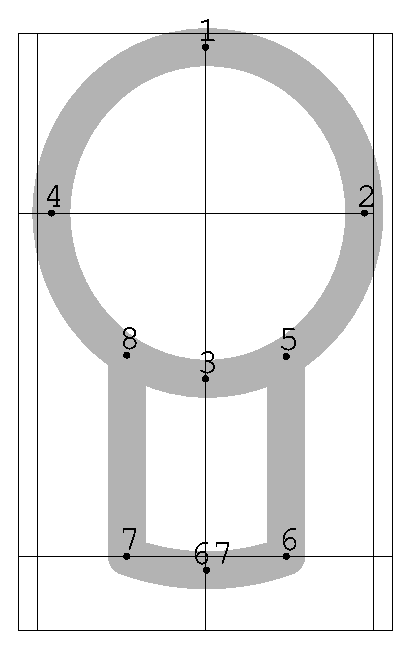
\includegraphics[height=6cm]{lightbulb.eps}
  \caption{Proof diagram of \filename{lightbulb10.mf}}
  \label{lightbulb10-proof}
\end{figure}

Most, if not all, \tex distributions include a Plain \tex file called
\testfonttex that is useful for testing new fonts in a variety of
ways.  One useful routine produces a table of all of the characters in
the font:

\bigskip
\noindent
\begingroup
\newcommand*{\usercmd}[1]{\textrm{\textbf{#1}}}%
\leftskip=\parindent \parindent=0pt \ttfamily \obeylines \obeyspaces%
\osprompt \usercmd{tex testfont}
This is TeX, Version 3.14159 (Web2C 7.3.1)
(/usr/share/texmf/tex/plain/base/testfont.tex
Name of the font to test = \usercmd{lightbulb10}
Now type a test command (\string\help for help):)
*\usercmd{\textbackslash{}table}
\vspace{\baselineskip}
*\usercmd{\textbackslash{}bye}
[1]
Output written on testfont.dvi (1 page, 1516 bytes).
Transcript written on testfont.log.
\endgroup
\bigskip

\noindent
The resulting table, stored in \filename{testfont.dvi} and illustrated
in \ref{font-table}, shows every character in the font.  To
understand how to read the table, note that the character code
for~``A''---the only character defined by
\filename{lightbulb10.mf}---is 41 in hexadecimal (base~16) and 101 in
octal (base~8).

\begin{figure}[htbp]
\centering
\fbox{%
\begin{minipage}{0.9\linewidth}
\centering
\vspace*{\baselineskip}
\begin{minipage}{0.95\linewidth}
{\tiny Test of lightbulb10 on March 11, 2003 at 1127}
\vspace{2\baselineskip}

\renewcommand{\tabularxcolumn}[1]{>{\mbox{}\hfill}p{#1}<{\hfill\mbox{}}}%
% The following two lines are modified from testfont.tex
\def\oct#1{\hbox{\normalfont\'{}\kern-.2em\itshape#1\/\kern.05em}} % octal constant
\def\hex#1{\hbox{\normalfont\H{}\ttfamily#1}} % hexadecimal constant

\begin{tabularx}{\linewidth}{@{}*9{X|}X@{}}
      & \oct{0} & \oct{1} & \oct{2} & \oct{3} &
        \oct{4} & \oct{5} & \oct{6} & \oct{7} & \\ \hline
 \oct{10x}
      &    & \lightbulb & & & & & & &
      \raisebox{-0.5\baselineskip}[0pt][0pt]{\hex{4x}} \\ \cline{1-9}
 \oct{11x}
      &    &            & & & & & & & \\ \hline
      & \hex{8} & \hex{9} & \hex{A} & \hex{B} &
        \hex{C} & \hex{D} & \hex{E} & \hex{F} & \\
\end{tabularx}
\end{minipage}
\vspace*{\baselineskip}
\end{minipage}}
\caption{Font table produced by \testfonttex}
\label{font-table}
\end{figure}

The LightBulb10 font is now usable by \tex.  \latexE, however, needs
more information before documents can use the font.  First, we create
a font-description file that tells \latexE how to map fonts in a given
\fntfam\ and encoding to a particular font in a particular font size.
For symbol fonts, this mapping is fairly simple.  Symbol fonts almost
always use the ``U''~(``Unknown'') font encoding and frequently occur
in only one variant: normal weight and non-\italic[italicized].  The
filename for a font-description file important; it must be of the form
``\meta{encoding}\meta{family}\fileext{fd}'', where \meta{encoding} is
the lowercase version of the encoding name (typically~``u'' for symbol
fonts) and \meta{family} is the name of the \fntfam.  For LightBulb10,
let's call this ``bulb''.  \ref{bulb-fd-file} lists the contents of
\filename{ubulb.fd}.  The document ``\latexE Font
Selection''~\cite{fntguide} describes \cmd{\DeclareFontFamily} and
\cmd{\DeclareFontShape} in detail, but the gist of \filename{ubulb.fd}
is first to declare a \texttt{U}-encoded version of the \texttt{bulb}
\fntfam[bulb] and then to specify that a \latexE request for a
\texttt{U}-encoded version of \texttt{bulb} with a (\texttt{m})edium
font series (as opposed to, e.g., bold) and a (\texttt{n})ormal font
shape (as opposed to, e.g., \italic) should translate into a \tex
request for \filename{lightbulb10.tfm}
mechanically\idxboth{mechanical}{scaling} scaled to the current font
size.

\begin{figure}[htbp]
\centering
\begin{tabular}{@{}|l|@{}}
  \hline
  \verb+\DeclareFontFamily{U}{bulb}{}+ \\
  \verb+\DeclareFontShape{U}{bulb}{m}{n}{<-> lightbulb10}{}+ \\
  \hline
\end{tabular}
\caption{\latexE font-description file (\filename{ubulb.fd})}
\label{bulb-fd-file}
\end{figure}

The final step is to write a \latexE style file that defines a name
for each symbol in the font.  Because we have only one symbol our
style file, \filename{lightbulb.sty} (\ref{bulb-sty-file}), is rather
trivial.  Note that instead of typesetting ``\texttt{A}'' we could
have had \cmdI{\lightbulb} typeset ``\cmd{\char}\texttt{65}'',
``\cmd{\char}\verb+"41+'', or ``\cmd{\char}\verb+'101+''
(respectively, decimal, hexadecimal, and octal character offsets into
the font).  For a simple, one-character symbol font such as
LightBulb10 it would be reasonable to merge \filename{ubulb.fd} into
\filename{lightbulb.sty} instead of maintaining two separate files.
In either case, a document need only include
``\verb+\usepackage{lightbulb}+'' to make the \verb+\lightbulb+ symbol
available.

\begin{figure}[htbp]
\centering
\begin{tabular}{@{}|l|@{}}
  \hline
  \verb+\newcommand{\lightbulb}{{\usefont{U}{bulb}{m}{n}A}}+ \\
  \hline
\end{tabular}
\caption{\latexE style file (\filename{lightbulb.sty})}
\label{bulb-sty-file}
\end{figure}

\bigskip

\metafont normally produces bitmapped fonts.  However, it is also
possible, with the help of some external tools, to produce \postscript
\PSfont{Type~1} fonts.  These have the advantages of rendering better
in Adobe\regtm\index{Adobe Acrobat} Acrobat\regtm (at least in
versions prior to~6.0) and of being more memory-efficient when handled
by a \postscript interpreter.  See \TeXFAQ{textrace} for pointers to
tools that can produce \PSfont{Type~1} fonts from \metafont.


\subsection{Math-mode spacing}
\label{math-spacing}

Terms such as ``binary operators'', ``relations'', and ``punctuation''
in \ref{math-symbols} primarily regard the surrounding
spacing.  (See the Short Math Guide for \latex~\cite{Downes:smg} for a
nice exposition on the subject.)  To use a symbol for a different
purpose, you can use the \tex commands \cmd{\mathord}, \cmd{\mathop},
\cmd{\mathbin}, \cmd{\mathrel}, \cmd{\mathopen}, \cmd{\mathclose}, and
\cmd{\mathpunct}.  For example, if you want to use \cmd{\downarrow} as
a variable (an ``ordinary'' symbol) instead of a delimiter, you can
write ``\verb|$3 x + \mathord{\downarrow}$|'' to get the properly
spaced ``$3 x + \mathord{\downarrow}$'' rather than the
awkward-looking ``$3 x + \downarrow$''.  Similarly, to create a
dotted-union\index{dotted union=dotted union ($\dot\cup$)} symbol
(``$\dot\cup$'') that spaces like the ordinary set-union symbol
(\cmdX{\cup}) it must be defined with \cmd{\mathbin}, just as
\cmdX{\cup} is.  Contrast ``\verb|$A \dot{\cup} B$|'' (``$A {\dot\cup}
B$'') with ``\verb|$A \mathbin{\dot{\cup}} B$|'' (``$A
\mathbin{\dot{\cup}} B$'').  See \TeXbook for the definitive
description of math-mode spacing.

The purpose of the ``log-like symbols'' in
\ifAMS
  \ref{log} and~\ref{ams-log}
\else
  \ref{log}
\fi
is to provide the correct amount of spacing around and within
multiletter function names.  \vref{log-spacing} contrasts the
output of the log-like symbols with various, na\"{\i}ve alternatives.
In addition to spacing, the log-like symbols also handle subscripts
properly.  For example, ``\verb|\max_{p \in P}|'' produces ``$\max_{p
\in P}$'' in text, but ``$\displaystyle\max_{p \in P}$'' as part of a
displayed formula.

\begin{nonsymtable}{Spacing Around/Within Log-like Symbols}
\label{log-spacing}
\setlength{\tabcolsep}{1em}
\begin{tabular}{@{}ll@{}} \toprule
\latex{} expression & Output \\ \midrule
\verb|$r \sin \theta$|         & $r \sin \theta$ \rlap{\quad (best)} \\
\verb|$r sin \theta$|          & $r sin \theta$          \\
\verb|$r \mbox{sin} \theta$|   & $r \mbox{sin} \theta$   \\
\verb|$r \mathrm{sin} \theta$| & $r \mathrm{sin} \theta$ \\
\bottomrule
\end{tabular}
\end{nonsymtable}

The \pkgname{amsmath} package makes it straightforward to define new
log-like symbols:

\begin{verbatim}
   \DeclareMathOperator{\atan}{atan}
   \DeclareMathOperator*{\lcm}{lcm}
\end{verbatim}
\ifAMS
  \indexcommand[$\string\atan$]{\atan}%
  \indexcommand[$\string\lcm$]{\lcm}
\else
  \indexcommand{\atan}%
  \indexcommand{\lcm}
\fi   % AMS test

\noindent
The difference between \cmd{\DeclareMathOperator} and
\cmd{\DeclareMathOperator*} involves the handling of subscripts.  With
\cmd{\DeclareMathOperator*}, subscripts are written beneath log-like
symbols in display style and to the right in text style.  This is
useful for limit operators (e.g.,~\cmdX{\lim}) and functions that tend
to map over a set (e.g.,~\cmdX{\min}).  In contrast,
\cmd{\DeclareMathOperator} tells \tex that subscripts should always be
displayed to the right of the operator, as is common for functions
that take a single parameter (e.g.,~\cmdX{\log} and~\cmdX{\cos}).
\ref{new-log-likes} contrasts symbols declared with
\cmd{\DeclareMathOperator} and \cmd{\DeclareMathOperator*} in both
text style~(\texttt{\$}$\ldots$\texttt{\$}) and
display~style~(\texttt{\string\[}$\ldots$\texttt{\string\]}).\footnote{Note
that \cmd{\displaystyle} can be used to force display style
within~\texttt{\$}$\ldots$\texttt{\$} and \cmd{\textstyle} can be used
to force text style
within~\texttt{\string\[}$\ldots$\texttt{\string\]}.}

\begin{nonsymtable}{Defining new log-like symbols}
\label{new-log-likes}
\renewcommand{\tabcolsep}{1em}
\begin{tabular}{@{}lll@{}}
  \toprule
  Declaration function &
  \texttt{\$\string\newlogsym\_\string{p \string\in~P\string}\$} &
  \texttt{\string\[~\string\newlogsym\_\string{p \string\in~P\string}~\string\]} \\
  \midrule

  \texttt{\string\DeclareMathOperator} &
  $\newlogsym_{p \in P}$ &
  $\displaystyle\newlogsym_{p \in P}$ \\[1ex]

  \texttt{\string\DeclareMathOperator*} &
  $\newlogsymSTAR_{p \in P}$ &
  $\displaystyle\newlogsymSTAR_{p \in P}$ \\
  \bottomrule
\end{tabular}
\end{nonsymtable}

It is common to use a thin\idxboth{thin}{space} space~(\cmd{\,})
between the words of a multiword operators, as in
``\verb|\DeclareMathOperator*|\linebreak[0]\verb|{\argmax}|\linebreak[0]\verb|{arg\,max}|''.
\cmdX{\liminf}, \cmdX{\limsup}, and all of the
log-like\idxboth{log-like}{symbols}\index{atomic math objects} symbols
shown in \ref{ams-log} utilize this spacing convention.


\subsection{Bold mathematical symbols}
\label{bold-math}

\idxbothbegin{bold}{symbols}

\latex\ does not normally use bold symbols when typesetting mathematics.
However, bold symbols are occasionally needed, for example when naming
vectors.  Any of the approaches described at \TeXFAQ{boldgreek} can be
used to produce bold mathematical symbols.  \ref{bold-symbols}
contrasts the output produced by these various techniques.  As the
table illustrates, these techniques exhibit variation in their
formatting of Latin letters (upright vs.\ \italic), formatting of
Greek\index{Greek>bold}\index{Greek>letters} letters (bold
vs.\ normal), formatting of operators and relations (bold
vs.\ normal), and spacing.
\ifXFB
  \pkgname{xfakebold}'s \cmd{\setBold} command is unique in that it takes a
  thickness argument and supports arbitrary symbol thickness, although it
  works only with vector fonts, not bitmapped fonts.
\fi

% The following was copied verbatim from amsbsy.sty.
\makeatletter
\DeclareRobustCommand{\pmb}{%
  \ifmmode\else \expandafter\pmb@@\fi\mathpalette\pmb@}
\def\pmb@@#1#2#3{\leavevmode\setboxz@h{#3}%
   \dimen@-\wdz@
   \kern-.5\ex@\copy\z@
   \kern\dimen@\kern.25\ex@\raise.4\ex@\copy\z@
   \kern\dimen@\kern.25\ex@\box\z@
}
\newdimen\pmbraise@
\def\pmb@#1#2{\setbox8\hbox{$\m@th#1{#2}$}%
  \setboxz@h{$\m@th#1\mkern.5mu$}\pmbraise@\wdz@
  \binrel@{#2}%
  \dimen@-\wd8 %
  \binrel@@{%
    \mkern-.8mu\copy8 %
    \kern\dimen@\mkern.4mu\raise\pmbraise@\copy8 %
    \kern\dimen@\mkern.4mu\box8 }%
}
\makeatother

\begin{nonsymtable}{Producing bold mathematical symbols}
  \idxboth{bold}{symbols}
  \label{bold-symbols}
  \begin{tabular}{@{}lll@{}}
    \toprule
    Package & Code & Output \\
    \midrule

    \textit{none} &
    \verb!$\alpha + b = \Gamma \div D$! &
    $\alpha + b = \Gamma \div D$ \rlap{\qquad (no bold)} \\

    \textit{none} &
    \verb!$!\cmd{\mathbf}\verb!{\alpha + b = \Gamma \div D}$! &
\ifBM
    $\alpha + \textbf{b} = \bm{\Gamma} \div \textbf{D}$ \\
\else
    $\mathbf{\alpha + b = \Gamma \div D}$ \\
\fi

    \textit{none} &
    \cmd{\boldmath}\verb!$\alpha + b = \Gamma \div D$! &
    \boldmath$\alpha + b = \Gamma \div D$ \\

    \pkgname{amsbsy} &
    \verb!$!\cmd{\pmb}\verb!{\alpha + b = \Gamma \div D}$! &
    $\pmb{\alpha + b = \Gamma \div D}$ \rlap{\qquad (faked bold)} \\

    \pkgname{amsbsy} &
    \verb!$!\cmd{\boldsymbol}\verb!{\alpha + b = \Gamma \div D}$! &
    \boldmath$\alpha + b = \Gamma \div D$ \\

\ifBM
    \pkgname{bm} &
    \verb!$!\cmd{\bm}\verb!{\alpha + b = \Gamma \div D}$! &
    $\bm{\alpha + b = \Gamma \div D}$ \\
\fi

    \pkgname{fixmath} &
    \verb!$!\cmd{\mathbold}\verb!{\alpha + b = \Gamma \div D}$! &
    \def\GammaIt{\mathord{\usefont{OML}{cmm}{b}{it}\mathchar"7100}}%
    \boldmath$\alpha + b = \GammaIt \div D$ \\

\ifXFB
    \pkgname{xfakebold} &
    \cmd{\setBold}\texttt{[0.3]}
    & \setBold[0.3]$\alpha + b = \Gamma \div D$\unsetBold
    \rlap{\qquad\kern3pt (faked bold)} \\
    & \verb!  $\alpha + b = \Gamma \div D$! \\
    & \verb!\unsetBold! \\
\fi
    \bottomrule
  \end{tabular}
\end{nonsymtable}

\idxbothend{bold}{symbols}


\subsection{ASCII and Latin~1 quick reference}
\label{ascii-quickref}

\index{ASCII|(}

\vref{ascii-table} amalgamates data from various other tables in this
document into a convenient reference for \latexE typesetting of \ascii
characters, i.e., the characters available on a typical U.S. computer
keyboard.  The first two columns list the character's \ascii code in
decimal and hexadecimal.  The third column shows what the character
looks like.  The fourth column lists the \latexE command to typeset
the character as a text character.  And the fourth column lists the
\latexE command to typeset the character within a
\verb|\texttt{|$\ldots$\verb|}| command (or, more generally, when
\verb|\ttfamily| is in effect).

\index{ASCII|)}

\begin{nonsymtable}{\latexE ASCII Table}
  \index{ASCII>table}
  \index{quotation marks}
  \label{ascii-table}
  % Define an equivalent of \vdots that's the height of a "9".
  \newlength{\digitheight}
  \settoheight{\digitheight}{9}
  \newcommand{\digitvdots}{\raisebox{-1.5pt}[\digitheight]{$\vdots$}}

  % Replace all glyphs in a row with vertical dots.
  \makeatletter
  \newcommand{\skipped}{%
    \settowidth{\@tempdima}{99} \makebox[\@tempdima]{\digitvdots} &
    \settowidth{\@tempdima}{99} \makebox[\@tempdima]{\digitvdots} &
    \digitvdots &
    \digitvdots &
    \digitvdots \\
  }
  \makeatother

  % Typesetting a symbol by prefixing it with a "\".
  \newcommand{\bscommand}[1]{#1 & \cmdI{#1} & \cmdI{#1}}

  \begin{tabular}[t]{@{}*2{>{\ttfamily}r}c*2{>{\ttfamily}l}l@{}} \\ \toprule
    \multicolumn{1}{@{}c}{Dec} &
    \multicolumn{1}{c}{Hex} &
    \multicolumn{1}{c}{Char} &
    \multicolumn{1}{c}{Body text} &
    \multicolumn{1}{c@{}}{\ttfamily\string\texttt} \\ \midrule

    33 & 21 & ! & ! & ! \\
    34 & 22 & {\fontencoding{T1}\selectfont\textquotedbl} &
      \string\textquotedbl & " \\      % Not available in OT1
    35 & 23 & \bscommand{\#} \\
    36 & 24 & \bscommand{\$} \\
    37 & 25 & \bscommand{\%} \\
    38 & 26 & \bscommand{\&} \\
    39 & 27 & ' & ' & ' \\
    40 & 28 & ( & ( & ( \\
    41 & 29 & ) & ) & ) \\
    42 & 2A & * & * & * \\
    43 & 2B & + & + & + \\
    44 & 2C & , & , & , \\
    45 & 2D & - & - & - \\
    46 & 2E & . & . & . \\
    47 & 2F & / & / & / \\
    48 & 30 & 0 & 0 & 0 \\
    49 & 31 & 1 & 1 & 1 \\
    50 & 32 & 2 & 2 & 2 \\
    \skipped
    57 & 39 & 9 & 9 & 9 \\
    58 & 3A & : & : & : \\
    59 & 3B & ; & ; & ; \\
    60 & 3C & \textless & \cmdI{\textless} & < \\         % Or $<$
    61 & 3D & = & = & = \\ \bottomrule
  \end{tabular}
  \hfil
  \begin{tabular}[t]{@{}*2{>{\ttfamily}r}c*2{>{\ttfamily}l}l@{}} \\ \toprule
    \multicolumn{1}{@{}c}{Dec} &
    \multicolumn{1}{c}{Hex} &
    \multicolumn{1}{c}{Char} &
    \multicolumn{1}{c}{Body text} &
    \multicolumn{1}{c@{}}{\ttfamily\string\texttt} \\ \midrule

    62 & 3E & \textgreater & \cmdI{\textgreater} & > \\   % Or $>$
    63 & 3F & ? & ? & ? \\
    64 & 40 & @ & @ & @ \\
    65 & 41 & A & A & A \\
    66 & 42 & B & B & B \\
    67 & 43 & C & C & C \\
    \skipped
    90 & 5A & Z & Z & Z \\
    91 & 5B & [ & [ & [ \\
    92 & 5C & \textbackslash & \cmdI{\textbackslash} &
      \verb|\char`\\| \\   % \textbackslash works in non-OT1
    93 & 5D & ] & ] & ] \\
    94 & 5E & \^{} & \verb|\^{}| & \verb|\^{}| \\   % Or \textasciicircum
    95 & 5F & \_ & \verb|\_| & \verb|\char`\_| \\   % \_ works in non-OT1
    96 & 60 & ` & ` & ` \\
    97 & 61 & a & a & a \\
    98 & 62 & b & b & b \\
    99 & 63 & c & c & c \\
    \skipped
   122 & 7A & z & z & z \\
   123 & 7B & \{ & \verb|\{| & \verb|\char`\{| \\   % \{ works in non-OT1
   124 & 7C & \textbar & \cmdI{\textbar} & | \\     % Or $|$
   125 & 7D & \} & \verb|\}| & \verb|\char`\}| \\   % \} works in non-OT1
   126 & 7E & \~{} & \verb|\~{}| & \verb|\~{}| \\   % Or \textasciitilde ($\sim$?)
   \\
   \bottomrule
  \end{tabular}
\end{nonsymtable}

The following are some additional notes about the contents of
\ref{ascii-table}:

\begin{itemize}
  \item
  ``\indexcommand[\string\encone{\string\textquotedbl}]{\textquotedbl}{\encone{\textquotedbl}}''
  is not available in the OT1 \fntenc[OT1].

  \item \ref{ascii-table} shows a close quote for character~39 for
    consistency with the open quote shown for character~96.  A
    straight quote can be typeset using \cmdI{\textquotesingle}
    (cf.~\ref{tc-misc}).

  \item
  The\label{upside-down}\index{symbols>upside-down|(}\index{upside-down
  symbols|(} characters ``\texttt{<}'', ``\texttt{>}'', and
  ``\texttt{|}'' do work as expected in math mode, although they
  produce, respectively, ``<'', ``>'', and ``|'' in text mode when
  using the OT1 \fntenc[OT1].\footnote{Donald\index{Knuth, Donald E.}
  Knuth didn't think such symbols were important outside of
  mathematics so he omitted them from his text fonts.} The following
  are some alternatives for typesetting ``\textless'',
  ``\textgreater'', and ``\textbar'':

  \begin{itemize}
    \item Specify a document \fntenc{} other than OT1 (as
    described~\vpageref[above]{altenc}).

    \item Use the appropriate symbol commands from
    \vref{text-predef}, viz.~\cmdI{\textless},
    \cmdI{\textgreater}, and \cmdI{\textbar}.

    \item Enter the symbols in math mode instead of text mode,
    i.e.,~\verb+$<$+, \verb+$>$+, and \verb+$|$+.
  \end{itemize}

  \noindent
  Note that for typesetting metavariables many people prefer
  \cmdI{\textlangle} and \cmdI{\textrangle} to \cmdI{\textless} and
  \cmdI{\textgreater}; i.e., ``\meta{filename}'' instead of
  ``$<$\textit{filename}$>$''.\index{symbols>upside-down|)}\index{upside-down
  symbols|)}

  \item Although ``\texttt{/}'' does not require any special
  treatment, \latex additionally defines a \cmdI{\slash} command which
  outputs the same glyph but permits a line~break afterwards.  That
  is, ``\texttt{increase/decrease}'' is always typeset as a single
  entity while ``\verb|increase\slash{}decrease|'' may be typeset with
  ``increase/'' on one line and ``decrease'' on the next.

  \item \label{page:tildes} \index{tilde|(} \cmdI{\textasciicircum}
  can be used instead of \cmdI[\string\^{}]{\^{}}\verb|{}|, and
  \cmdI{\textasciitilde} can be used instead of
  \cmdI[\string\~{}]{\~{}}\verb|{}|.  Note that
  \cmdI{\textasciitilde} and \cmdI[\string\~{}]{\~{}}\verb|{}|
  produce raised, diacritic tildes.  ``Text''
  (i.e.,~vertically\index{tilde>vertically centered} centered)
  tildes can be generated with either the math-mode \cmdX{\sim}
  command (shown in \vref{rel}), which produces a somewhat wide
  ``$\sim$'', or the \TC\ package's \cmdI{\texttildelow} (shown in
  \vref{tc-misc}), which produces a vertically centered
  ``{\fontfamily{ptm}\selectfont\texttildelow}'' in most fonts but a
  baseline-oriented ``\texttildelow'' in \PSfont{Computer Modern},
  \TX, \PX, and various other fonts originating from the
  \tex\ world.  If your goal is to typeset tildes in URLs or Unix
  filenames, your best bet is to use the \pkgname{url} package,
  which has a number of nice features such as proper line-breaking
  of such names.\index{tilde|)}

  \item The various \cmd{\char} commands within \verb|\texttt| are
  necessary only in the OT1 \fntenc[OT1].  In other encodings
  (e.g.,~T1)\index{font encodings>T1}, commands such as \cmdIp{\{},
  \cmdIp{\}}, \cmdI{\_}, and \cmdI{\textbackslash} all work properly.

  \item The code\index{code page 437} page~437 (IBM~PC\index{IBM PC})
  version of \ascii characters~1 to~31 can be typeset
  using the \ASCII\ package.
\ifASCII
  See \vref{ibm-ascii}.
\fi

  \item To replace~``\verb|`|'' and~``\verb|'|'' with the more
  computer-like (and more visibly distinct) ``\texttt{\char18}''
  and~``\texttt{\char13}'' within a \texttt{verbatim} environment,
  use the \pkgname{upquote} package.  Outside of \texttt{verbatim},
  you can use \cmd{\char}\texttt{18} and \cmd{\char}\texttt{13} to
  get the modified quote characters.  (The former is actually a
  grave accent.)
\end{itemize}

\index{Latin 1|(}

Similar to \ref{ascii-table}, \vref{latin1-table} is an amalgamation
of data from other tables in this document.  While \ref{ascii-table}
shows how to typeset the 7-bit \ascii character set,
\ref{latin1-table} shows the Latin~1 (Western European) character set,
also known as ISO-8859-1.

\index{Latin 1|)}

\begin{nonsymtable}{\latexE Latin~1 Table}
  \index{Latin 1}
  \index{copyright}
  \index{trademark}
  \idxboth{registered}{trademark}
  \idxboth{legal}{symbols}
  \label{latin1-table}

  \newcommand{\accented}[2]{#1#2 & \texttt{\string#1\string{#2\string}}}
  \newcommand{\idxencone}[1]{\indexcommand[\string\encone{\string#1}]{#1}\encone{#1}}
  \begin{tabular}[t]{@{}*2{>{\ttfamily}r}c>{\ttfamily}lc@{}} \\ \toprule
    \multicolumn{1}{@{}c}{Dec} &
    \multicolumn{1}{c}{Hex} &
    \multicolumn{1}{c}{Char} &
    \multicolumn{2}{c@{}}{\latexE} \\ \midrule

    161 & A1 & !`                 & !{}` \\
    162 & A2 & \textcent          & \cmdI{\textcent} & (\textsf{tc}) \\
    163 & A3 & \pounds            & \cmdI{\pounds} \\
    164 & A4 & \textcurrency      & \cmdI{\textcurrency} & (\textsf{tc}) \\
    165 & A5 & \textyen           & \cmdI{\textyen} & (\textsf{tc}) \\
    166 & A6 & \textbrokenbar     & \cmdI{\textbrokenbar} & (\textsf{tc}) \\
    167 & A7 & \S                 & \cmdI{\S} \\
    168 & A8 & \textasciidieresis & \cmdI{\textasciidieresis} & (\textsf{tc}) \\
    169 & A9 & \textcopyright     & \cmdI{\textcopyright} \\
    170 & AA & \textordfeminine   & \cmdI{\textordfeminine}   \\
    171 & AB & \idxencone{\guillemetleft} & \string\guillemetleft & (T1) \\
    172 & AC & \textlnot          & \cmdI{\textlnot} & (\textsf{tc}) \\
    173 & AD & -                  & \cmdI[-]{\-} \\
    174 & AE & \textregistered    & \cmdI{\textregistered} \\
    175 & AF & \textasciimacron   & \cmdI{\textasciimacron} & (\textsf{tc}) \\
    176 & B0 & \textdegree        & \cmdI{\textdegree} & (\textsf{tc}) \\
    177 & B1 & \textpm            & \cmdI{\textpm} & (\textsf{tc}) \\
    178 & B2 & \texttwosuperior   & \cmdI{\texttwosuperior} & (\textsf{tc}) \\
    179 & B3 & \textthreesuperior & \cmdI{\textthreesuperior} & (\textsf{tc}) \\
    180 & B4 & \textasciiacute    & \cmdI{\textasciiacute} & (\textsf{tc}) \\
    181 & B5 & \textmu            & \cmdI{\textmu} & (\textsf{tc}) \\
    182 & B6 & \P                 & \cmdI{\P} \\
    183 & B7 & \textperiodcentered & \cmdI{\textperiodcentered} \\
    184 & B8 & \c{}               & \cmdI[\string\blackacchack{\string\c}]{\c}\verb|{}| \\
    185 & B9 & \textonesuperior   & \cmdI{\textonesuperior} & (\textsf{tc}) \\
    186 & BA & \textordmasculine  & \cmdI{\textordmasculine} \\
    187 & BB & \idxencone{\guillemetright} & \string\guillemetright & (T1) \\
    188 & BC & \textonequarter    & \cmdI{\textonequarter} & (\textsf{tc}) \\
    189 & BD & \textonehalf       & \cmdI{\textonehalf} & (\textsf{tc}) \\
    190 & BE & \textthreequarters & \cmdI{\textthreequarters} & (\textsf{tc}) \\
    191 & BF & ?`                 & ?{}` \\
    192 & C0 & \accented{\`}{A} \\
    193 & C1 & \accented{\'}{A} \\
    194 & C2 & \accented{\^}{A} \\
    195 & C3 & \accented{\~}{A} \\
    196 & C4 & \accented{\"}{A} \\
    197 & C5 & \usefont{OT1}{cmr}{m}{n}\AA
                                  & \string\AA \\
    198 & C6 & \AE                & \string\AE \\
    199 & C7 & \accented{\c}{C} \\
    200 & C8 & \accented{\`}{E} \\
    201 & C9 & \accented{\'}{E} \\
    202 & CA & \accented{\^}{E} \\
    203 & CB & \accented{\"}{E} \\
    204 & CC & \accented{\`}{I} \\
    205 & CD & \accented{\'}{I} \\
    206 & CE & \accented{\^}{I} \\
    207 & CF & \accented{\"}{I} \\
    208 & D0 & \idxencone{\DH}    & \string\DH & (T1) \\ \bottomrule
  \end{tabular}
  \hfil
  \begin{tabular}[t]{@{}*2{>{\ttfamily}r}c>{\ttfamily}lc@{}} \\ \toprule
    \multicolumn{1}{@{}c}{Dec} &
    \multicolumn{1}{c}{Hex} &
    \multicolumn{1}{c}{Char} &
    \multicolumn{2}{c@{}}{\latexE} \\ \midrule

    209 & D1 & \accented{\~}{N} \\
    210 & D2 & \accented{\`}{O} \\
    211 & D3 & \accented{\'}{O} \\
    212 & D4 & \accented{\^}{O} \\
    213 & D5 & \accented{\~}{O} \\
    214 & D6 & \accented{\"}{O} \\
    215 & D7 & \texttimes         & \string\texttimes & (\textsf{tc}) \\
    216 & D8 & \O                 & \string\O \\
    217 & D9 & \accented{\`}{U} \\
    218 & DA & \accented{\'}{U} \\
    219 & DB & \accented{\^}{U} \\
    220 & DC & \accented{\"}{U} \\
    221 & DD & \accented{\'}{Y} \\
    222 & DE & \idxencone{\TH}    & \string\TH & (T1) \\
    223 & DF & \ss                & \string\ss \\
    224 & E0 & \accented{\`}{a} \\
    225 & E1 & \accented{\'}{a} \\
    226 & E2 & \accented{\^}{a} \\
    227 & E3 & \accented{\~}{a} \\
    228 & E4 & \accented{\"}{a} \\
    229 & E5 & \usefont{OT1}{cmr}{m}{n}\aa
                                  & \string\aa \\
    230 & E6 & \ae                & \string\ae \\
    231 & E7 & \accented{\c}{c} \\
    232 & E8 & \accented{\`}{e} \\
    233 & E9 & \accented{\'}{e} \\
    234 & EA & \accented{\^}{e} \\
    235 & EB & \accented{\"}{e} \\
    236 & EC & \accented{\`}{\i} \\
    237 & ED & \accented{\'}{\i} \\
    238 & EE & \accented{\^}{\i} \\
    239 & EF & \accented{\"}{\i} \\
    240 & F0 & \idxencone{\dh}    & \string\dh & (T1) \\
    241 & F1 & \accented{\~}{n} \\
    242 & F2 & \accented{\`}{o} \\
    243 & F3 & \accented{\'}{o} \\
    244 & F4 & \accented{\^}{o} \\
    245 & F5 & \accented{\~}{o} \\
    246 & F6 & \accented{\"}{o} \\
    247 & F7 & \textdiv           & \string\textdiv & (\textsf{tc}) \\
    248 & F8 & \o                 & \string\o \\
    249 & F9 & \accented{\`}{u} \\
    250 & FA & \accented{\'}{u} \\
    251 & FB & \accented{\^}{u} \\
    252 & FC & \accented{\"}{u} \\
    253 & FD & \accented{\'}{y} \\
    254 & FE & \idxencone{\th}    & \string\th & (T1) \\
    255 & FF & \accented{\"}{y} \\ \bottomrule
  \end{tabular}
\end{nonsymtable}

The following are some additional notes about the contents of
\ref{latin1-table}:

\begin{itemize}
  \item A ``(\textsf{tc})'' after a symbol name means that the \TC\
  package must be loaded to access that symbol.  A ``(T1)'' means that
  the symbol requires the T1 \fntenc[T1].  The \pkgname{fontenc}
  package can change the \fntenc[document] document-wide.

  \item Many of the \verb|\text|\dots\ accents can also be produced
  using the accent commands shown in \vref{text-accents} plus an
  empty argument.  For instance,
  \verb|\={}|\index{_=\magicequalname{}\verb+{}+ (\magicequal{})}
  is essentially the same as \cmd{\textasciimacron}.

  \item The commands in the ``\latexE'' columns work both in body text
  and within a \verb|\texttt{|$\ldots$\verb|}| command (or, more
  generally, when \verb|\ttfamily| is in effect).

  \item The ``\pounds'' and ``\$'' glyphs occupy the same slot~(36) of
  the OT1 \fntenc[OT1], with ``\pounds'' appearing in \italic\ fonts and
  ``\$'' appearing in roman fonts.  A problem with \latex's default
  handling of this double-mapping is that
  ``\texttt{\string{\string\sffamily\linebreak[0]\string\slshape\linebreak[0]\string\pounds\string}}''
  produces
  ``{\fontencoding{OT1}\sffamily\slshape\selectfont\textdollar}'', not
  ``{\fontencoding{T1}\sffamily\slshape\selectfont\textsterling}''.
  Other \fntenc{}s use separate slots for the two characters and are
  therefore robust to the problem of ``\pounds''/''\$'' conflicts.
  Authors who use \cmdI{\pounds} should select a \fntenc{} other than
  OT1 (as explained~\vpageref[above]{altenc}) or use the \TC\ package,
  which redefines \cmdI{\pounds} to use the TS1 \fntenc[TS1].

  \item Character~173, \cmdI[-]{\-}, is shown as ``-'' but is actually
  a discretionary\index{discretionary hyphen}\index{hyphen,
  discretionary} hyphen; it appears only at the end of a line.
\end{itemize}

\index{code page 1252|(}
Microsoft\regtm\index{Microsoft Windows=Microsoft\regtm\
Windows\regtm} Windows\regtm\index{Windows=Windows\regtm} normally
uses a superset of Latin~1 called ``Code Page~1252'' or ``CP1252'' for
short.  CP1252 introduces symbols in the Latin~1 ``invalid'' range
(characters~128--159).  \ref{cp1252-table} presents the
characters with which CP1252 augments the standard Latin~1\index{Latin
1} table.
\index{code page 1252|)}

\begin{nonsymtable}{\latexE Code Page~1252 Table}
  \index{code page 1252>table}
  \index{quotation marks}
  \index{trademark}
  \label{cp1252-table}
  \newcommand{\accented}[2]{#1#2 & \texttt{\string#1\string{#2\string}}}
  \newcommand{\idxencone}[1]{\indexcommand[\string\encone{\string#1}]{#1}\encone{#1}}

  \begin{tabular}[t]{@{}*2{>{\ttfamily}r}c>{\ttfamily}lc@{}} \\ \toprule
    \multicolumn{1}{@{}c}{Dec} &
    \multicolumn{1}{c}{Hex} &
    \multicolumn{1}{c}{Char} &
    \multicolumn{2}{c@{}}{\latexE} \\ \midrule
    128 & 80 & \texteuro          & \cmdI{\texteuro} & (\textsf{tc}) \\
    130 & 82 & \idxencone{\quotesinglbase} & \string\quotesinglbase & (T1) \\
    131 & 83 & \textit{f}         & \verb|\textit{f}| \\
    132 & 84 & \idxencone{\quotedblbase}   & \string\quotedblbase & (T1) \\
    133 & 85 & \dots              & \cmdI{\dots} \\
    134 & 86 & \dag               & \cmdI{\dag} \\
    135 & 87 & \ddag              & \cmdI{\ddag} \\
    136 & 88 & \textasciicircum   & \cmdI{\textasciicircum} \\
    137 & 89 & \textperthousand   & \cmdI{\textperthousand} & (\textsf{tc}) \\
    138 & 8A & \accented{\v}{S}   \\
    139 & 8B & \idxencone{\guilsinglleft}  & \string\guilsinglleft & (T1) \\
    140 & 8C & \OE                & \cmdI{\OE} \\
    142 & 8E & \accented{\v}{Z}   \\
    \bottomrule
  \end{tabular}
  \hfil
  \begin{tabular}[t]{@{}*2{>{\ttfamily}r}c>{\ttfamily}lc@{}} \\ \toprule
    \multicolumn{1}{@{}c}{Dec} &
    \multicolumn{1}{c}{Hex} &
    \multicolumn{1}{c}{Char} &
    \multicolumn{2}{c@{}}{\latexE} \\ \midrule
    145 & 91 & `                  & ` \\
    146 & 92 & '                  & ' \\
    147 & 93 & ``                 & `` \\
    148 & 94 & ''                 & '' \\
    149 & 95 & \textbullet        & \cmdI{\textbullet} \\
    150 & 96 & --                 & -- \\
    151 & 97 & ---                & --- \\
    152 & 98 & \textasciitilde    & \cmdI{\textasciitilde} \\
    153 & 99 & \texttrademark     & \cmdI{\texttrademark} \\
    154 & 9A & \accented{\v}{s}   \\
    155 & 9B & \idxencone{\guilsinglright}  & \string\guilsinglright & (T1) \\
    156 & 9C & \oe                & \cmdI{\oe} \\
    158 & 9E & \accented{\v}{z}   \\
    159 & 9F & \accented{\"}{Y}   \\
    \bottomrule
  \end{tabular}
\end{nonsymtable}

The following are some additional notes about the contents of
\ref{cp1252-table}:

\begin{itemize}
  \item As in \ref{latin1-table}, a ``(\textsf{tc})'' after a
  symbol name means that the \TC\ package must be loaded to access
  that symbol.  A ``(T1)'' means that the symbol requires the T1
  \fntenc[T1].  The \pkgname{fontenc} package can change the
  \fntenc[document] document-wide.

  \item Not all characters in the 128--159 range are defined.

  \item Look up ``euro signs'' in the index for alternatives to
  \cmdI{\texteuro}.
\end{itemize}

\index{ISO character entities|(}
\setpkgnameopts{isoent}{link=http://www.bitjungle.com/isoent/}
While too large to incorporate into this document, a listing of
ISO~8879:1986 SGML\index{SGML}/XML\index{XML} character entities and their
\latex{} equivalents is available from
\url{http://www.bitjungle.com/isoent/}.  Some of the characters presented
there make use of \pkgname{isoent}, a \latexE{} package (available from the
same URL) that fakes some of the missing ISO glyphs using the
\latex\ \texttt{picture} environment.\footnote{\pkgname{isoent} is not
  featured in this document, because it is not available from \CTAN and
  because the faked symbols are not ``true'' characters; they exist in only
  one size, regardless of the body text's font size.}
\index{ISO character entities|)}


\subsection{Unicode characters}
\label{unicode-chars}

\index{Unicode|(}

\href{http://www.unicode.org/}{Unicode} is a ``universal character
set''---a standard for encoding (i.e.,~assigning unique numbers to)
the symbols appearing in many of the world's languages.  While \ascii
can represent 128 symbols and Latin~1 can represent 256 symbols,
Unicode can represent an astonishing 1,114,112 symbols.

Because \tex and \latex{} predate the Unicode standard and Unicode
fonts by almost a decade, support for Unicode has had to be added to
the base \tex{} and \latex{} systems.  Note first that \latex{}
distinguishes between \emph{input} encoding---the characters used in
the \fileext{tex} file---and \emph{output} encoding---the characters
that appear in the generated \fileext{dvi}, \fileext{pdf}, etc.\ file.

\subsubsection{Inputting Unicode characters}

To include Unicode characters in a \fileext{tex} file, load the
\pkgname[pkg=unicode]{ucs} package and load the \pkgname{inputenc} package
with the \optname{inputenc}{utf8x} (``\utfviii extended'')
option.\footnote{\utfviii is the 8-bit Unicode Transformation Format,
  a popular mechanism for representing Unicode symbol numbers as
  sequences of one to four bytes.}  These packages enable \latex{} to
translate \utfviii sequences to \latex{} commands, which are
subsequently processed as normal.  For example, the \utfviii text
``\texttt{Copyright~\textcopyright\ \the\year}''---``\texttt{\textcopyright}''
is not an \ascii character and therefore cannot be input directly
without packages such as
\pkgname[pkg=unicode]{ucs}/\pkgname{inputenc}---is converted internally by
\pkgname{inputenc} to ``\texttt{Copyright} \verb+\textcopyright{}+
\texttt{\the\year}'' and therefore typeset as
``Copyright~\textcopyright\ \the\year''.

The \pkgname[pkg=unicode]{ucs}\slash\pkgname{inputenc} combination
supports only a tiny subset of Unicode's million-plus symbols.
Additional symbols can be added manually using the
\cmd{\DeclareUnicodeCharacter} command.
\cmd{\DeclareUnicodeCharacter} takes two arguments: a Unicode number
and a \latex{} command to execute when the corresponding Unicode
character is encountered in the input.  For example, the Unicode
character ``degree celsius''~(``\,\textcelsius\,'') appears at
character position U+2103.\footnote{The Unicode convention is to
  express character positions as ``U+\meta{hexadecimal number}''.}
However, ``\,\texttt{\textcelsius}\,'' is not one of the characters
that \pkgname[pkg=unicode]{ucs} and \pkgname{inputenc} recognize.  The
following document shows how to use \cmd{\DeclareUnicodeCharacter} to
tell \latex{} that the ``\,\texttt{\textcelsius}\,'' character should
be treated as a synonym for \cmdI{\textcelsius}:

\begin{verbatim}
   \documentclass{article}
   \usepackage{ucs}
   \usepackage[utf8x]{inputenc}
   \usepackage{textcomp}

   \DeclareUnicodeCharacter{"2103}{\textcelsius}   % Enable direct input of U+2103.
\end{verbatim}
\noindent
\verb|   \begin{document}| \\
\verb|   |\texttt{It was a balmy 21\textcelsius.} \\
\verb|   \end{document}|

\bigskip

\noindent
which produces

\begin{quotation}
  It was a balmy 21\textcelsius.
\end{quotation}

\seedocs{\pkgname[pkg=unicode]{ucs}} and for descriptions of the various
options that control \pkgname[pkg=unicode]{ucs}'s behavior.


\subsubsection{Outputting Unicode characters}

Orthogonal to the ability to include Unicode characters in a
\latex\ input file is the ability to include a given Unicode character
in the corresponding output file.  By far the easiest approach is to
use \xelatex instead of pdf\LaTeX\index{pdfLaTeX=pdf\LaTeX} or
ordinary \latex.  \xelatex handles Unicode input and output natively
and can utilize system fonts directly without having to expose them
via \fileext{tfm}, \fileext{fd}, and other such files.  To output a
Unicode character, a \xelatex document can either include that
character directly as \utfviii text or use \tex's \cmd{\char}
primitive, which \xelatex extends to accept numbers larger than~255.

\ifJUNI
  \newcommand{\versicleIDX}{\index{versicle=versicle (\versicle)}}
  \newcommand{\responseIDX}{\index{response=response (\response)}}
\else
  \newcommand{\versicleIDX}{\index{versicle}}
  \newcommand{\responseIDX}{\index{response}}
\fi

Suppose we want to output the symbols for
\ifJUNI
  versicle\versicleIDX~(``\versicle'') and response\responseIDX~(``\response'')
\else
  versicle\versicleIDX{} and response\responseIDX{}
\fi
in a document.  The \href{http://www.unicode.org/charts/}{Unicode
  charts} list ``versicle\versicleIDX'' at position~U+2123 and
``response\responseIDX'' at position~U+211F\@.  We therefore need to
install a font that contains those characters at their proper
positions.  One such font that is freely available from \CTAN is
Junicode
(\hfilename{http://mirror.ctan.org/fonts/junicode/fonts/Junicode.ttf}{Junicode.ttf})
from the \JUNI\ package.  The \pkgname{fontspec} package makes it easy
for a \xelatex document to utilize a system font.  The following
example defines a \texttt{\string\textjuni} command that uses
\pkgname{fontspec} to typeset its argument in Junicode:

\begin{verbatim}
   \documentclass{article}
   \usepackage{fontspec}

   \newcommand{\textjuni}[1]{{\fontspec{Junicode}#1}}

   \begin{document}
   We use ``\textjuni{\char"2123}'' for a versicle
   and ``\textjuni{\char"211F}'' for a response.
   \end{document}
\end{verbatim}

\ifJUNI
  \noindent
  which produces

  \begin{quotation}
    We use ``\versicle'' for a versicle\versicleIDX\ and ``\response''
    for a response\responseIDX.
  \end{quotation}
\fi

\noindent
(Typesetting the entire document in Junicode would be even easier.
\seedocs{\pkgname{fontspec}} regarding font selection.)  Note how the
preceding example uses \cmd{\char} to specify a Unicode character by
number.  The double quotes before the number indicate that the number
is represented in hexadecimal instead of decimal.

\index{Unicode|)}


\subsection{About this document}
\label{about-doc}

\paragraph{History}
\person{David}{Carlisle} wrote the first version of this document in
October, 1994.  It originally contained all of the native \latex{}
symbols (\ref{bin}, \ref{op}, \ref{rel}, \ref{arrow}, \ref{log},
\ref{greek}, \ref{dels}, \ref{ldels}, \ref{math-accents},
\ref{extensible-accents}, \ref{ord}, and a few tables that have since
been reorganized) and was designed to be nearly identical to the
tables in Chapter~3 of Leslie\index{Lamport, Leslie} Lamport's
book~\cite{Lamport:latex}.  Even the table captions and the order of
the symbols within each table matched!  The \AMS\ symbols
(\ref{ams-bin}, \ref{ams-rel}, \ref{ams-nrel}, \ref{ams-arrows},
\ref{ams-narrows}, \ref{ams-greek}, \ref{ams-hebrew}, \ref{ams-del},
and \ref{ams-misc}) and an initial Math Alphabets table
(\ref{alphabets}) were added thereafter.  Later,
\person{Alexander}{Holt} provided the \ST\ tables (\ref{st-bin},
\ref{st-large}, \ref{st-rel}, \ref{st-arrows}, \ref{st-ext}, and
\ref{st-del}).

In January, 2001, \person{Scott}{Pakin} took responsibility for
maintaining the symbol list and has since implemented a complete
overhaul of the document.  The result, now called, ``The \doctitle'',
includes the following new features:

\begin{itemize}
  \item the addition of a handful of new math alphabets, dozens of new
  font tables, and thousands of new symbols

  \item the categorization of the symbol tables into body-text
  symbols, mathematical symbols, science and technology symbols,
  dingbats, ancient languages, and other symbols, to provide a more
  user-friendly document structure

  \item an index, table of contents, hyperlinks, and a
  frequently-requested symbol list, to help users quickly locate
  symbols

  \item symbol tables rewritten to list the symbols in alphabetical
  order

  \item appendices providing additional information relevant to using
  symbols in \latex{}

  \item tables showing how to typeset all of the characters in the
    \ascii and Latin~1\index{Latin 1}
    \fntenc[ASCII]s\index{font encodings>Latin 1}
\end{itemize}

\noindent
Furthermore, the internal structure of the document has been
completely altered from \person{David}{Carlisle}'s original version.
Most of the changes are geared towards making the document easier to
extend, modify, and reformat.


\paragraph{Build characteristics}
\vref{doc-characteristics} lists some of this document's build
characteristics.  Most important is the list of packages that \latex{}
couldn't find, but that \selftex otherwise would have been able to
take advantage of.  Complete, prebuilt versions of this document are
available from \CTAN\ via
\url{https://www.ctan.org/pkg/comprehensive/}.  \ref{package-dates}
shows the package date (specified in the \verb|.sty|~file with
\cmd{\ProvidesPackage}) for each package that was used to build this
document and that specifies a package date.  Packages are not listed
in any particular order in either \ref{doc-characteristics}
or~\ref{package-dates}.

\begin{nonsymtable}{Document Characteristics}
\label{doc-characteristics}
\bgroup
  \sffamily
  \xdef\orighyphenchar{\the\hyphenchar\font}
  \hyphenchar\font=-1
\egroup
\begin{tabular}{@{}lp{0.5\textwidth}@{}} \toprule
Characteristic      & Value \\ \midrule
Source file:        & \selftex \\
Build date:         & \today \\
Symbols documented: & \approxcount\prevtotalsymbols \\
Packages included:  & \makeatletter
                        \def\@elt#1{\pkgname{#1}\xspace}
                        \foundpkgs
                      \makeatother \\
Packages omitted:   & \makeatletter
                        \ifcomplete
                          \emph{none}
                        \else
                          \def\@elt#1{\pkgname{#1}\xspace}
                          \missingpkgs
                        \fi
                      \makeatother \\
\bottomrule
\end{tabular}
\bgroup
  \sffamily
  \hyphenchar\font=\orighyphenchar
\egroup
\end{nonsymtable}


% Automatically generate a table of package version numbers.
\ifhaveplaceins
  \FloatBarrier
\else
  \clearpage
\fi
\makeatletter
\begingroup
  % Given a package name, output the package's date.
  \def\show@package@date#1/#2/#3#4#5!!!{#1/#2/#3#4}
  \newcommand{\showpackagedate}[1]{{%
    \catcode`\&=12% yfonts.sty obnoxiously uses an unescaped "&" in the package description.
    \xdef\package@date@string{\csname ver@#1.sty\endcsname}%
    \expandafter\show@package@date\package@date@string!!!
  }}

  % Toggle between "&" and "\\".
  \global\newcount\pkg@column
  \gdef\pkg@end@entry{%
    \global\advance\pkg@column by 1\relax
    \ifnum\pkg@column=3\relax
      \let\next=\LT@tabularcr
      \global\pkg@column=0\relax
    \else
      \def\next{&&}%
    \fi
    \next
  }

  % Produce the entire table body as a token list.
  \newtoks\pkg@date@toks
  \def\@elt#1{%
    \expandafter\ifx\csname ver@#1.sty\endcsname\relax
    \else
      \expandafter\ifx\csname ver@#1.sty\endcsname\@empty
      \else
        \pkgname{#1} & \showpackagedate{#1} \pkg@end@entry
      \fi
    \fi
  }
  \expandafter\pkg@date@toks\expandafter=\expandafter{\foundpkgs}

  % Output a formatted table that contains the previously defined token list.
  \begin{longnonsymtable}{Package versions used in the preparation of this document}
  \label{package-dates}
  \begin{longtable}{@{}lr*2{clr}@{}}
    \multicolumn{8}{@{}l@{}}{%
      \makebox[0pt][l]{\small\textit{(continued from previous page)}}} \\[3ex]
    \toprule
    Name & \multicolumn{1}{l}{Date} & \qquad &
    Name & \multicolumn{1}{l}{Date} & \qquad &
    Name & \multicolumn{1}{l@{}}{Date} \\
    \cmidrule(r){1-2}\cmidrule(lr){4-5}\cmidrule(l){7-8}
    \endhead
    \toprule
    Name & \multicolumn{1}{l}{Date} & \qquad &
    Name & \multicolumn{1}{l}{Date} & \qquad &
    Name & \multicolumn{1}{l@{}}{Date} \\
    \cmidrule(r){1-2}\cmidrule(lr){4-5}\cmidrule(l){7-8}
    \endfirsthead
    \bottomrule
    \\[1ex]
    \multicolumn{8}{@{}r@{}}{%
      \makebox[0pt][r]{\small\textit{(continued on next page)}}}
    \endfoot
    \endlastfoot
    \the\pkg@date@toks
    \\
    \bottomrule
  \end{longtable}
  \end{longnonsymtable}
\endgroup
\makeatother


\subsection{Copyright and license}

\noindent
\begin{tabular}{@{}l@{}}
  The \doctitle \\
  Copyright~\copyright\ 2007--\number\year, Scott Pakin \\
\end{tabular}

\bigskip

\noindent
This work may be distributed and/or modified under the conditions of
the \latex\ Project Public License, either version~1.3c of this license
or (at your option) any later version.  The latest version of this
license is in

\begin{center}
  \url{http://www.latex-project.org/lppl.txt}
\end{center}

\noindent
and version~1.3c or later is part of all distributions of \latex\
version 2006/05/20 or later.

\bigskip

This work has the LPPL maintenance status ``maintained''.

\bigskip

The current maintainer of this work is Scott Pakin.

\ifTWEM
  \bigskip

  The Twitter emoji graphics provided by \TWEM\ are licensed under
  \href{https://creativecommons.org/licenses/by/4.0/}{CC-BY 4.0}.
  Copyright~\copyright\ 2019 Twitter, Inc.\ and other contributors.
\fi

% It seems like such a waste to put such a brief bibliography on its own
% page.  So we temporarily restore \section back to its original
% definition, just for the list of references.

\vspace{\stretch{1}}
\begingroup
\let\section=\origsection

\realsections
\begin{thebibliography}{Knu86b}

\bibitem[AMS99]{AMS1999:amsmath}
  American Mathematical Society.
  \emph{User's Guide for the \textsf{amsmath} Package (Version~2.0)},
  December~13, 1999.
  Available from \url{ftp://ftp.ams.org/pub/tex/doc/amsmath/amsldoc.pdf}.

\bibitem[Ber01]{Berry:fontname}
  Karl Berry.\index{Berry, Karl}
  Fontname: Filenames for \tex fonts,
  June 2001.
  Available from \url{https://www.ctan.org/pkg/fontname}.

\bibitem[Che98]{Chen1998}
  Raymond Chen.\index{Chen, Raymond}
  A \MF\ of `Simpsons' characters.
  \emph{Baskerville}, 4(4):19, February 1998.
  ISSN~\mbox{1354-5930}.
  Available from
  \url{http://uk.tug.org/wp-installed-content/uploads/2008/12/44.pdf}.

\bibitem[Dow00]{Downes:smg}
  Michael Downes.\index{Downes, Michael J.}
  Short math guide for {\latex},
  July~19, 2000.
  Version~1.07.
  Available from \url{http://www.ams.org/tex/short-math-guide.html}.

\bibitem[Gib97]{Gibbons:longdiv}
  Jeremy Gibbons.\index{Gibbons, Jeremy}
  Hey---it works!
  \emph{\TUGboat}, 18(2):75--78, June 1997.
  Available from \url{http://www.tug.org/TUGboat/Articles/tb18-2/tb55works.pdf}.

\bibitem[Gre09]{Gregorio2009:latex-book}
  Enrico Gregorio.
  \emph{Appunti di programmazione in \latex e \TeX},
  second edition, June 2009.  Available from
    \url{http://profs.sci.univr.it/~gregorio/introtex.pdf}.

\bibitem[Knu86a]{Knuth:ct-a}
  Donald~E. Knuth.\index{Knuth, Donald E.}
  \emph{The {\TeX}book},
  volume~A of \emph{Computers and Typesetting}.
  Ad{\-d}i{\-s}on-Wes{\-l}ey,
  Reading, MA, USA,
  1986.

\bibitem[Knu86b]{Knuth:ct-c}
  Donald~E. Knuth.\index{Knuth, Donald E.}
  \emph{The {\MF}book},
  volume~C of \emph{Computers and Typesetting}.
  Ad{\-d}i{\-s}on-Wes{\-l}ey,
  Reading, MA, USA,
  1986.

\bibitem[Lam86]{Lamport:latex}
  Leslie Lamport.\index{Lamport, Leslie}
  \emph{\latex: A document preparation system}.
  Ad{\-d}i{\-s}on-Wes{\-l}ey,
  Reading, MA, USA,
  1986.

\bibitem[\LaT{}98]{ltnews09}
  \latex{}3~Project Team.
  A new math accent.
  \emph{\latex News}. Issue~9, June~1998.
  Available from
  \url{https://www.latex-project.org/news/latex2e-news/ltnews09.pdf}
  and also included in many \tex{} distributions.

\bibitem[\LaT{}19]{fntguide}
  \latex{}3~Project Team.
  \latexE font selection,
  October 2019.
  Available from
  \url{http://mirrors.ctan.org/macros/latex/base/fntguide.pdf}
  and also included in many \tex{} distributions.
\end{thebibliography}
\endgroup

% "See also"s should appear after all page references.
\providecommand*\seealso[2]{\emph{\alsoname}#1}
\providecommand*\alsoname{see also}
\index{carriage return|seealso{\texttt{\string\hookleftarrow}}}
\index{transforms|seealso{alphabets, math}}
\ifKEYS
  \index{enter|seealso{carriage return}}
\else
  \index{enter|see{carriage return}}
\fi

\clearpage
\realsections
\phantomsection
\addcontentsline{toc}{section}{Index}
\bgroup
  \def\pkgnameopts{index=false}%
  \small
  \printindex
\egroup

\end{document}
